% !Mode:: "TeX:UTF-8"
% !TEX encoding = UTF-8 Unicode

%----------------------------------------------------------------------------------------
% 机器翻译:统计建模与深度学习方法
% Machine Translation: Statistical Modeling and Deep Learning Methods
%
% Copyright 2020
% 肖桐(xiaotong@mail.neu.edu.cn) 朱靖波 (zhujingbo@mail.neu.edu.cn)
%----------------------------------------------------------------------------------------

%----------------------------------------------------------------------------------------
%	BASIC CONFIGURATIONS
%----------------------------------------------------------------------------------------

\documentclass[11pt]{book} % font and book template
% !Mode:: "TeX:UTF-8"
% !TEX encoding = UTF-8 Unicode

%%%%%%%%%%%%%%%%%%%%%%%%%%%%%%%%%%%%%%%%%
% This file was modified on top of 
% The Legrand Orange Book
% Structural Definitions File
%
% Original author:
% Mathias Legrand (legrand.mathias@gmail.com) with modifications by:
% Vel (vel@latextemplates.com)
%
% Current Version is maintained by 
% Tong Xiao (xiaotong@mail.neu.edu.cn)
% Runzhe Cao (854581319@qq.com)
%
% License of This File:
% CC BY-NC-SA 4.0 (http://creativecommons.org/licenses/by-nc-sa/4.0/)
%
%%%%%%%%%%%%%%%%%%%%%%%%%%%%%%%%%%%%%%%%%

%----------------------------------------------------------------------------------------
%	VARIOUS REQUIRED PACKAGES AND CONFIGURATIONS
%----------------------------------------------------------------------------------------

\usepackage{graphicx} % Required for including pictures
\graphicspath{{Figures/}} % Specifies the directory where pictures are stored

\usepackage{lipsum} % Inserts dummy text

\usepackage{tikz} % Required for drawing custom shapes

\usepackage[english]{babel} % English language/hyphenation

\usepackage{enumitem} % Customize lists
\setlist{nolistsep} % Reduce spacing between bullet points and numbered lists

\usepackage{booktabs} % Required for nicer horizontal rules in tables

\usepackage{xcolor} % Required for specifying colors by name
\definecolor{ocre}{RGB}{243,102,25} % Define the orange color used for highlighting throughout the book

%----------------------------------------------------------------------------------------
%	MARGINS
%----------------------------------------------------------------------------------------

\usepackage{geometry} % Required for adjusting page dimensions and margins

\geometry{
	paper=b5paper, % Paper size, change to letterpaper for US letter size
	%papersize={185mm,260mm}, % specify paper size by (width,height)
	top=2cm, % Top margin
	bottom=1.5cm, % Bottom margin原来1.5cm
	left=1.8cm, % Left margin
	right=1.8cm, % Right margin
	headheight=10pt, % Header height
	footskip=1.4cm, % Space from the bottom margin to the baseline of the footer
	headsep=10pt, % Space from the top margin to the baseline of the header
	%showframe, % Uncomment to show how the type block is set on the page
}

%----------------------------------------------------------------------------------------
%	FONTS
%----------------------------------------------------------------------------------------

\usepackage{avant} % Use the Avantgarde font for headings
%\usepackage{times} % Use the Times font for headings
\usepackage{mathptmx} % Use the Adobe Times Roman as the default text font together with math symbols from the Sym­bol, Chancery and Com­puter Modern fonts

\usepackage{microtype} % Slightly tweak font spacing for aesthetics
\usepackage[utf8]{inputenc} % Required for including letters with accents
\usepackage[T1]{fontenc} % Use 8-bit encoding that has 256 glyphs


%----------------------------------------------------------------------------------------
%	BIBLIOGRAPHY AND INDEX
%----------------------------------------------------------------------------------------

\usepackage[style=numeric,citestyle=numeric,sorting=anyt,sortcites=true,maxbibnames=40,minbibnames=30,autopunct=true,babel=hyphen,hyperref=true,abbreviate=false,backref=true,backend=biber]{biblatex}
%maxbibnames 设置参考文献最多显示作者数目
%minbibnames 如果作者数目超过maxbibnames,则只显示minbibnames个作者
\addbibresource{bibliography.bib} % BibTeX bibliography file
\defbibheading{bibempty}{}

\usepackage{calc} % For simpler calculation - used for spacing the index letter headings correctly
\usepackage{makeidx} % Required to make an index
\makeindex % Tells LaTeX to create the files required for indexing
\newcommand{\upcite}[1]{\textsuperscript{\textsuperscript{\cite{#1}}}}%参考文献上标

%----------------------------------------------------------------------------------------
%	MAIN TABLE OF CONTENTS
%----------------------------------------------------------------------------------------

\usepackage{titletoc} % Required for manipulating the table of contents

\contentsmargin{0cm} % Removes the default margin

% Part text styling (this is mostly taken care of in the PART HEADINGS section of this file)
\titlecontents{part}
	[0cm] % Left indentation
	{\addvspace{20pt}\bfseries} % Spacing and font options for parts
	{}
	{}
	{}

% Chapter text styling
\titlecontents{chapter}
	[1.25cm] % Left indentation
	{\addvspace{12pt}\large\sffamily\bfseries} % Spacing and font options for chapters
	{\color{ocre!60}\contentslabel[\Large\thecontentslabel]{1.25cm}\color{ocre}} % Formatting of numbered sections of this type
	{\color{ocre}} % Formatting of numberless sections of this type
	{\color{ocre!60}\normalsize\;\titlerule*[.5pc]{.}\;\thecontentspage} % Formatting of the filler to the right of the heading and the page number

% Section text styling
\titlecontents{section}
	[1.25cm] % Left indentation
	{\addvspace{3pt}\sffamily\bfseries} % Spacing and font options for sections
	{\contentslabel[\thecontentslabel]{1.25cm}} % Formatting of numbered sections of this type
	{} % Formatting of numberless sections of this type
	{\titlerule*[.5pc]{.}\;\thecontentspage}%
	%{\hfill\color{black}\thecontentspage} % Formatting of the filler to the right of the heading and the page number
% Subsection text styling
\titlecontents{subsection}
	[1.25cm] % Left indentation
	{\addvspace{1pt}\sffamily\small} % Spacing and font options for subsections
	{\contentslabel[\thecontentslabel]{1.25cm}} % Formatting of numbered sections of this type
	{} % Formatting of numberless sections of this type
	{\ \titlerule*[.5pc]{.}\;\thecontentspage} % Formatting of the filler to the right of the heading and the page number

% Figure text styling
\titlecontents{figure}
	[1.25cm] % Left indentation
	{\addvspace{1pt}\sffamily\small} % Spacing and font options for figures
	{\thecontentslabel\hspace*{1em}} % Formatting of numbered sections of this type
	{} % Formatting of numberless sections of this type
	{\ \titlerule*[.5pc]{.}\;\thecontentspage} % Formatting of the filler to the right of the heading and the page number

% Table text styling
\titlecontents{table}
	[1.25cm] % Left indentation
	{\addvspace{1pt}\sffamily\small} % Spacing and font options for tables
	{\thecontentslabel\hspace*{1em}} % Formatting of numbered sections of this type
	{} % Formatting of numberless sections of this type
	{\ \titlerule*[.5pc]{.}\;\thecontentspage} % Formatting of the filler to the right of the heading and the page number

%----------------------------------------------------------------------------------------
%	MINI TABLE OF CONTENTS IN PART HEADS
%----------------------------------------------------------------------------------------

% Chapter text styling
\titlecontents{lchapter}
	[0em] % Left indentation
	{\addvspace{15pt}\large\sffamily\bfseries} % Spacing and font options for chapters
	{\color{ocre}\contentslabel[\Large\thecontentslabel]{1.25cm}\color{ocre}} % Chapter number
	{}
	{\color{ocre}\normalsize\sffamily\bfseries\;\titlerule*[.5pc]{.}\;\thecontentspage} % Page number

% Section text styling
\titlecontents{lsection}
	[0em] % Left indentation
	{\sffamily\small} % Spacing and font options for sections
	{\contentslabel[\thecontentslabel]{1.25cm}} % Section number
	{}
	{}

% Subsection text styling (note these aren't shown by default, display them by searchings this file for tocdepth and reading the commented text)
\titlecontents{lsubsection}
	[.5em] % Left indentation
	{\sffamily\footnotesize} % Spacing and font options for subsections
	{\contentslabel[\thecontentslabel]{1.25cm}}
	{}
	{}

%----------------------------------------------------------------------------------------
%	HEADERS AND FOOTERS
%----------------------------------------------------------------------------------------

\usepackage{fancyhdr} % Required for header and footer configuration

\pagestyle{fancy} % Enable the custom headers and footers

\renewcommand{\chaptermark}[1]{\markboth{\sffamily\normalsize\bfseries\chaptername\ \thechapter.\ #1 \quad 肖桐\ 朱靖波}{}} % Styling for the current chapter in the header
\renewcommand{\sectionmark}[1]{\markright{\sffamily\normalsize\thesection\hspace{5pt}#1}{}} % Styling for the current section in the header

\fancyhf{} % Clear default headers and footers
\fancyhead[LE,RO]{\sffamily\normalsize\thepage} % Styling for the page number in the header
\fancyhead[LO]{\rightmark} % Print the nearest section name on the left side of odd pages
\fancyhead[RE]{\leftmark} % Print the current chapter name on the right side of even pages
%\fancyfoot[RE]{\tiny{肖桐\ 朱靖波}}
%O-odd page,E-even page,R-right area,L-left area,C-center area
%\fancyfoot[C]{\thepage} % Uncomment to include a footer底部中间页码

\renewcommand{\headrulewidth}{0.5pt} % Thickness of the rule under the header

\fancypagestyle{plain}{% Style for when a plain pagestyle is specified
	\fancyhead{}\renewcommand{\headrulewidth}{0pt}%
}

% Removes the header from odd empty pages at the end of chapters
\makeatletter
\renewcommand{\cleardoublepage}{
\clearpage\ifodd\c@page\else
\hbox{}
\vspace*{\fill}
\thispagestyle{empty}
\newpage
\fi}

%----------------------------------------------------------------------------------------
%	THEOREM STYLES
%----------------------------------------------------------------------------------------

\usepackage{amsmath,amsfonts,amssymb,amsthm} % For math equations, theorems, symbols, etc

\newcommand{\intoo}[2]{\mathopen{]}#1\,;#2\mathclose{[}}
\newcommand{\ud}{\mathop{\mathrm{{}d}}\mathopen{}}
\newcommand{\intff}[2]{\mathopen{[}#1\,;#2\mathclose{]}}
\renewcommand{\qedsymbol}{$\blacksquare$}
\newtheorem{notation}{Notation}[chapter]

% Boxed/framed environments
\newtheoremstyle{ocrenumbox}% Theorem style name
{0pt}% Space above
{0pt}% Space below
{\normalfont}% Body font
{}% Indent amount
{\small\bf\sffamily\color{ocre}}% Theorem head font
{\;}% Punctuation after theorem head
{0.25em}% Space after theorem head
{\small\sffamily\color{ocre}\thmname{#1}\nobreakspace\thmnumber{\@ifnotempty{#1}{}\@upn{#2}}% Theorem text (e.g. Theorem 2.1)
\thmnote{\nobreakspace\the\thm@notefont\sffamily\bfseries\color{black}---\nobreakspace#3.}} % Optional theorem note

\newtheoremstyle{blacknumex}% Theorem style name
{5pt}% Space above
{5pt}% Space below
{\normalfont}% Body font
{} % Indent amount
{\small\bf\sffamily}% Theorem head font
{\;}% Punctuation after theorem head
{0.25em}% Space after theorem head
{\small\sffamily{\tiny\ensuremath{\blacksquare}}\nobreakspace\thmname{#1}\nobreakspace\thmnumber{\@ifnotempty{#1}{}\@upn{#2}}% Theorem text (e.g. Theorem 2.1)
\thmnote{\nobreakspace\the\thm@notefont\sffamily\bfseries---\nobreakspace#3.}}% Optional theorem note

\newtheoremstyle{blacknumbox} % Theorem style name
{0pt}% Space above
{0pt}% Space below
{\normalfont}% Body font
{}% Indent amount
{\small\bf\sffamily}% Theorem head font
{\;}% Punctuation after theorem head
{0.25em}% Space after theorem head
{\small\sffamily\thmname{#1}\nobreakspace\thmnumber{\@ifnotempty{#1}{}\@upn{#2}}% Theorem text (e.g. Theorem 2.1)
\thmnote{\nobreakspace\the\thm@notefont\sffamily\bfseries---\nobreakspace#3.}}% Optional theorem note

% Non-boxed/non-framed environments
\newtheoremstyle{ocrenum}% Theorem style name
{5pt}% Space above
{5pt}% Space below
{\normalfont}% Body font
{}% Indent amount
{\small\bf\sffamily\color{ocre}}% Theorem head font
{\;}% Punctuation after theorem head
{0.25em}% Space after theorem head
{\small\sffamily\color{ocre}\thmname{#1}\nobreakspace\thmnumber{\@ifnotempty{#1}{}\@upn{#2}}% Theorem text (e.g. Theorem 2.1)
\thmnote{\nobreakspace\the\thm@notefont\sffamily\bfseries\color{black}---\nobreakspace#3.}} % Optional theorem note
\makeatother

% Defines the theorem text style for each type of theorem to one of the three styles above
\newcounter{dummy}
\numberwithin{dummy}{section}
\theoremstyle{ocrenumbox}
\newtheorem{theoremeT}[dummy]{Theorem}
\newtheorem{problem}{Problem}[chapter]
\newtheorem{exerciseT}{Example}[chapter]
\theoremstyle{blacknumex}
\newtheorem{exampleT}{实例}[chapter]
\theoremstyle{blacknumbox}
\newtheorem{vocabulary}{Vocabulary}[chapter]
\newtheorem{definitionT}{定义}[section]
\newtheorem{corollaryT}[dummy]{Corollary}
\theoremstyle{ocrenum}
\newtheorem{proposition}[dummy]{Proposition}

%----------------------------------------------------------------------------------------
%	DEFINITION OF COLORED BOXES
%----------------------------------------------------------------------------------------

\RequirePackage[framemethod=default]{mdframed} % Required for creating the theorem, definition, exercise and corollary boxes

% Theorem box
\newmdenv[skipabove=7pt,
skipbelow=7pt,
backgroundcolor=black!5,
linecolor=ocre,
innerleftmargin=5pt,
innerrightmargin=5pt,
innertopmargin=5pt,
leftmargin=0cm,
rightmargin=0cm,
innerbottommargin=5pt]{tBox}

% Exercise box	
\newmdenv[skipabove=7pt,
skipbelow=7pt,
rightline=false,
leftline=true,
topline=false,
bottomline=false,
backgroundcolor=ocre!10,
linecolor=ocre,
innerleftmargin=5pt,
innerrightmargin=5pt,
innertopmargin=5pt,
innerbottommargin=5pt,
leftmargin=0cm,
rightmargin=0cm,
linewidth=4pt]{eBox}	

% Definition box
\newmdenv[skipabove=7pt,
skipbelow=7pt,
rightline=false,
leftline=true,
topline=false,
bottomline=false,
linecolor=ocre,
innerleftmargin=5pt,
innerrightmargin=5pt,
innertopmargin=0pt,
leftmargin=0cm,
rightmargin=0cm,
linewidth=4pt,
innerbottommargin=0pt]{dBox}	

% Corollary box
\newmdenv[skipabove=7pt,
skipbelow=7pt,
rightline=false,
leftline=true,
topline=false,
bottomline=false,
linecolor=gray,
backgroundcolor=black!5,
innerleftmargin=5pt,
innerrightmargin=5pt,
innertopmargin=5pt,
leftmargin=0cm,
rightmargin=0cm,
linewidth=4pt,
innerbottommargin=5pt]{cBox}

% Creates an environment for each type of theorem and assigns it a theorem text style from the "Theorem Styles" section above and a colored box from above
\newenvironment{theorem}{\begin{tBox}\begin{theoremeT}}{\end{theoremeT}\end{tBox}}
\newenvironment{exercise}{\begin{eBox}\begin{exerciseT}}{\hfill{\color{ocre}\tiny\ensuremath{\blacksquare}}\end{exerciseT}\end{eBox}}				
\newenvironment{definition}{\begin{dBox}\begin{definitionT}}{\end{definitionT}\end{dBox}}	
\newenvironment{example}{\begin{exampleT}}{\hfill{\tiny\ensuremath{\blacksquare}}\end{exampleT}}		
\newenvironment{corollary}{\begin{cBox}\begin{corollaryT}}{\end{corollaryT}\end{cBox}}	

%----------------------------------------------------------------------------------------
%	REMARK ENVIRONMENT
%----------------------------------------------------------------------------------------

\newenvironment{remark}{\par\vspace{10pt}\small % Vertical white space above the remark and smaller font size
\begin{list}{}{
\leftmargin=35pt % Indentation on the left
\rightmargin=25pt}\item\ignorespaces % Indentation on the right
\makebox[-2.5pt]{\begin{tikzpicture}[overlay]
\node[draw=ocre!60,line width=1pt,circle,fill=ocre!25,font=\sffamily\bfseries,inner sep=2pt,outer sep=0pt] at (-15pt,0pt){\textcolor{ocre}{R}};\end{tikzpicture}} % Orange R in a circle
\advance\baselineskip 1pt}{\end{list}\vskip5pt} % Tighter line spacing and white space after remark

%----------------------------------------------------------------------------------------
%	SECTION NUMBERING IN THE MARGIN
%----------------------------------------------------------------------------------------
%调整各级标题的段前段后间距
\makeatletter
\renewcommand{\@seccntformat}[1]{\llap{\textcolor{ocre}{\csname the#1\endcsname}\hspace{1em}}}
\renewcommand{\section}{\@startsection{section}{1}{\z@}
{-4ex \@plus -1ex \@minus -.4ex}
{1ex \@plus.2ex }
{\color{ublue}\normalfont\Large\sffamily\bfseries}}
\renewcommand{\subsection}{\@startsection {subsection}{2}{\z@}
{-3ex \@plus -0.1ex \@minus -.4ex}
{0.5ex \@plus.2ex }
{\normalfont\large\sffamily\bfseries}}
\renewcommand{\subsubsection}{\@startsection {subsubsection}{3}{\z@}
{-3ex \@plus -0.1ex \@minus -.4ex}
{.4ex \@plus.2ex }
{\normalfont\normalsize\sffamily\bfseries}}
\renewcommand\paragraph{\@startsection{paragraph}{4}{\z@}
{-2ex \@plus-.2ex \@minus .2ex}
{.1ex}
{\normalfont\small\sffamily\bfseries}}

%----------------------------------------------------------------------------------------
%	PART HEADINGS
%----------------------------------------------------------------------------------------

% Numbered part in the table of contents
\newcommand{\@mypartnumtocformat}[2]{%
	\setlength\fboxsep{0pt}%
	\noindent\colorbox{ocre!20}{\strut\parbox[c][.7cm]{\ecart}{\color{ocre!70}\Large\sffamily\bfseries\centering#1}}\hskip\esp\colorbox{ocre!40}{\strut\parbox[c][.7cm]{\linewidth-\ecart-\esp}{\Large\sffamily\centering#2}}%
}

% Unnumbered part in the table of contents
\newcommand{\@myparttocformat}[1]{%
	\setlength\fboxsep{0pt}%
	\noindent\colorbox{ocre!40}{\strut\parbox[c][.7cm]{\linewidth}{\Large\sffamily\centering#1}}%
}

\newlength\esp
\setlength\esp{4pt}
\newlength\ecart
\setlength\ecart{1.2cm-\esp}
\newcommand{\thepartimage}{}%
\newcommand{\partimage}[1]{\renewcommand{\thepartimage}{#1}}%
\def\@part[#1]#2{%
\ifnum \c@secnumdepth >-2\relax%
\refstepcounter{part}%
\addcontentsline{toc}{part}{\texorpdfstring{\protect\@mypartnumtocformat{\thepart}{#1}}{\partname~\thepart\ ---\ #1}}
\else%
\addcontentsline{toc}{part}{\texorpdfstring{\protect\@myparttocformat{#1}}{#1}}%
\fi%
\startcontents%
\markboth{}{}%
{\thispagestyle{empty}%
\begin{tikzpicture}[remember picture,overlay]%
\node at (current page.north west){\begin{tikzpicture}[remember picture,overlay]%	
\fill[ocre!20](0cm,0cm) rectangle (\paperwidth,-\paperheight);
\node[anchor=north] at (4cm,-3.25cm){\color{ocre!40}\fontsize{220}{100}\sffamily\bfseries\thepart};
\node[anchor=south east] at (\paperwidth-1cm,-\paperheight+1cm){\parbox[t][][t]{8.5cm}{
\printcontents{l}{0}{\setcounter{tocdepth}{1}}% The depth to which the Part mini table of contents displays headings; 0 for chapters only, 1 for chapters and sections and 2 for chapters, sections and subsections
}};
\node[anchor=north east] at (\paperwidth-1.5cm,-3.25cm){\parbox[t][][t]{15cm}{\strut\raggedleft\color{white}\fontsize{30}{30}\sffamily\bfseries#2}};
\end{tikzpicture}};
\end{tikzpicture}}%
\@endpart}
\def\@spart#1{%
\startcontents%
\phantomsection
{\thispagestyle{empty}%
\begin{tikzpicture}[remember picture,overlay]%
\node at (current page.north west){\begin{tikzpicture}[remember picture,overlay]%	
\fill[ocre!20](0cm,0cm) rectangle (\paperwidth,-\paperheight);
\node[anchor=north east] at (\paperwidth-1.5cm,-3.25cm){\parbox[t][][t]{15cm}{\strut\raggedleft\color{white}\fontsize{30}{30}\sffamily\bfseries#1}};
\end{tikzpicture}};
\end{tikzpicture}}
\addcontentsline{toc}{part}{\texorpdfstring{%
\setlength\fboxsep{0pt}%
\noindent\protect\colorbox{ocre!40}{\strut\protect\parbox[c][.7cm]{\linewidth}{\Large\sffamily\protect\centering #1\quad\mbox{}}}}{#1}}%
\@endpart}
\def\@endpart{\vfil\newpage
\if@twoside
\if@openright
\null
\thispagestyle{empty}%
\newpage
\fi
\fi
\if@tempswa
\twocolumn
\fi}

%----------------------------------------------------------------------------------------
%	SPECIAL FONTS
%----------------------------------------------------------------------------------------

\newcommand\bfnew[1]{\sffamily\bfseries{#1}}

%----------------------------------------------------------------------------------------
%	CHAPTER HEADINGS
%----------------------------------------------------------------------------------------

% A switch to conditionally include a picture, implemented by Christian Hupfer
\newif\ifusechapterimage
\usechapterimagetrue
\newcommand{\thechapterimage}{}%
\newcommand{\chapterimage}[1]{\ifusechapterimage\renewcommand{\thechapterimage}{#1}\fi}%
\newcommand{\autodot}{.}
\def\@makechapterhead#1{%
{\parindent \z@ \raggedright \normalfont
\ifnum \c@secnumdepth >\m@ne
\if@mainmatter
\begin{tikzpicture}[remember picture,overlay]
\node at (current page.north west)
{\begin{tikzpicture}[remember picture,overlay]
\node[anchor=north west,inner sep=0pt] at (0,0) {\ifusechapterimage\includegraphics[width=\paperwidth]{\thechapterimage}\fi};
\draw[anchor=west] (\Gm@lmargin,-7cm) node [line width=2pt,rounded corners=15pt,draw=ocre,fill=white,fill opacity=0.5,inner sep=15pt]{\strut\makebox[22cm]{}};
\draw[anchor=west] (\Gm@lmargin+.3cm,-7cm) node {\huge\sffamily\bfseries\color{black}\thechapter\autodot~#1\strut};
\end{tikzpicture}};
\end{tikzpicture}
\else
\begin{tikzpicture}[remember picture,overlay]
\node at (current page.north west)
{\begin{tikzpicture}[remember picture,overlay]
\node[anchor=north west,inner sep=0pt] at (0,0) {\ifusechapterimage\includegraphics[width=\paperwidth]{\thechapterimage}\fi};
\draw[anchor=west] (\Gm@lmargin,-7cm) node [line width=2pt,rounded corners=15pt,draw=ocre,fill=white,fill opacity=0.5,inner sep=15pt]{\strut\makebox[22cm]{}};
\draw[anchor=west] (\Gm@lmargin+.3cm,-7cm) node {\huge\sffamily\bfseries\color{black}#1\strut};
\end{tikzpicture}};
\end{tikzpicture}
\fi\fi\par\vspace*{270\p@}}}

%-------------------------------------------

\def\@makeschapterhead#1{%
\begin{tikzpicture}[remember picture,overlay]
\node at (current page.north west)
{\begin{tikzpicture}[remember picture,overlay]
\node[anchor=north west,inner sep=0pt] at (0,0) {\ifusechapterimage\includegraphics[width=\paperwidth]{\thechapterimage}\fi};
\draw[anchor=west] (\Gm@lmargin,-7cm) node [line width=2pt,rounded corners=15pt,draw=ocre,fill=white,fill opacity=0.5,inner sep=15pt]{\strut\makebox[22cm]{}};
\draw[anchor=west] (\Gm@lmargin+.3cm,-7cm) node {\huge\sffamily\bfseries\color{black}#1\strut};
\end{tikzpicture}};
\end{tikzpicture}
\par\vspace*{270\p@}}
\makeatother

%----------------------------------------------------------------------------------------
%	LINKS
%----------------------------------------------------------------------------------------

\usepackage{hyperref}
\hypersetup{hidelinks,backref=true,pagebackref=true,hyperindex=true,colorlinks=false,breaklinks=true,urlcolor=ocre,bookmarks=true,bookmarksopen=true}
%backref反向引用
%pagebackref反向引用页码
%hyperindex索引链接
%colorlinks彩色链接
%breaklinks允许链接断行
%urlcolor网页与电邮链接颜色
%bookmarks生成书签
%bookmarksopen书签目录展开

\usepackage{bookmark}
\bookmarksetup{
open,
numbered,
depth=2, %设置PDF的书签级别,2显示到subsection,3显示到subsubsection
addtohook={%
\ifnum\bookmarkget{level}=0 % chapter
\bookmarksetup{bold}%
\fi
\ifnum\bookmarkget{level}=-1 % part
\bookmarksetup{color=ocre,bold}%
\fi
}
}

%----------------------------------------------------------------------------------------
%	NEW PAGE FOR SUBSECTION
%----------------------------------------------------------------------------------------
%\newcommand{\sectionnewpage}{\clearpage}
\newcommand{\sectionnewpage}{}

%----------------------------------------------------------------------------------------
%	Chapter 3
%----------------------------------------------------------------------------------------
\usepackage{tikz}
\usetikzlibrary{arrows,decorations.pathreplacing}
\usetikzlibrary{positioning,fit,calc}
\usetikzlibrary{shadows} % LATEX and plain TEX when using Tik Z
\usetikzlibrary{mindmap,backgrounds} % mind map
\usepackage{type1cm}%设置公式字体
\usepackage{caption}%设置图片标题字体大小
\captionsetup{font={footnotesize}}
\usepackage{pstricks}
\DeclareMathOperator*{\argmax}{arg\,max}
\DeclareMathOperator*{\argmin}{arg\,min}
\usepackage{setspace}%调整行间距

%\usepackage{tocbibind}

%----------------------------------------------------------------------------------------
%	Chapter 1
%----------------------------------------------------------------------------------------
\usepackage{chngpage}
\usepackage[justification=centering]{caption}%强制图片居中
\usepackage{subfigure}
\newcommand{\parinterval}{\noindent\hspace{2em}}%定义变量替代原来开头的控制缩进
\usepackage{tikz-qtree}

\usepackage{array}
\usepackage{booktabs}
\usepackage{bm}
\usetikzlibrary{shapes.misc}
\usepackage{appendix}
\usepackage{pgfplots}
\usepackage{tikz}

%----------------------------------------------------------------------------------------
%	Chapter 4
%----------------------------------------------------------------------------------------
\usepackage{pgffor}%图片中使用\foreach语句

%----------------------------------------------------------------------------------------
%	Chapter 6
%----------------------------------------------------------------------------------------
\usepackage{multirow}
\usepackage{tcolorbox}
\newcommand{\dash}{\raisebox{0.5mm}{------}}%中文破折号
\usepackage{colortbl} %table上色

\newlength{\base}
\newdimen\XCoord
\newdimen\YCoord
\newdimen\TMP
\newcommand*{\ExtractCoordinate}[1]{\path (#1); \pgfgetlastxy{\XCoord}{\YCoord};}%
\newcommand*{\ExtractX}[1]{\path (#1); \pgfgetlastxy{\XCoord}{\TMP};}%
\newcommand*{\ExtractY}[1]{\path (#1); \pgfgetlastxy{\TMP}{\YCoord};}%
\newcommand{\specialcell}[3][c]{%
 \begin{tabular}[#1]{@{}#2@{}}#3\end{tabular}}

\usetikzlibrary{calc,intersections}
\usetikzlibrary{matrix}
\usetikzlibrary{patterns}
\usetikzlibrary{shadows.blur}
\usepgflibrary{arrows}
%\usetikzlibrary{arrows}
%\usetikzlibrary{decorations}
\usetikzlibrary{arrows,shapes}

%%%%%%%%%%%chapter5图片等---------------------------------------
\usepackage{tikz-3dplot}
\usepackage{pifont}
\tcbuselibrary{skins}
\definecolor{ublue}{rgb}{0.152,0.250,0.545}
\definecolor{ugreen}{rgb}{0,0.5,0}
\definecolor{lgreen}{rgb}{0.9,1,0.8}
\definecolor{xtgreen1}{rgb}{0.824,0.898,0.8}
\definecolor{xtgreen}{rgb}{0.914,0.945,0.902}
\definecolor{lightgray}{gray}{0.85}

%%%%%%%%%%%%appendix-------------------------------
\makeatletter
\def\UrlAlphabet{%
      \do\a\do\b\do\c\do\d\do\e\do\f\do\g\do\h\do\i\do\j%
      \do\k\do\l\do\m\do\n\do\o\do\p\do\q\do\r\do\s\do\t%
      \do\u\do\v\do\w\do\x\do\y\do\z\do\A\do\B\do\C\do\D%
      \do\E\do\F\do\G\do\H\do\I\do\J\do\K\do\L\do\M\do\N%
      \do\O\do\P\do\Q\do\R\do\S\do\T\do\U\do\V\do\W\do\X%
      \do\Y\do\Z}
\def\UrlDigits{\do\1\do\2\do\3\do\4\do\5\do\6\do\7\do\8\do\9\do\0}
\g@addto@macro{\UrlBreaks}{\UrlOrds}%特殊符号
\g@addto@macro{\UrlBreaks}{\UrlAlphabet}%26个字母表
\g@addto@macro{\UrlBreaks}{\UrlDigits}%10个阿拉伯数字
\makeatother
%上述设置的作用是URL自动换行

%%%%%%%%%%%chapter 7---------------------------------------
%\definecolor{myblack}{rgb}{0.15,0.15,0.15}
\definecolor{myblack}{rgb}{0.2,0.2,205.2}
\newlength{\hseg}
\newlength{\wnode}
\newlength{\hnode}
\newlength{\wseg}
\usepackage{collcell}
\usepackage[mathscr]{euscript}

 % self-defined template

\usepackage{hyperref}
%\hypersetup{pdftitle={Title},pdfauthor={Author}} % Uncomment and fill out to include PDF metadata for the author and title of the book

\usepackage {xeCJK}
\usepackage{ctex}
\setCJKmainfont{SimSun}
\setCJKmonofont{SimSun}
\setmainfont{Times New Roman}

%----------------------------------------------------------------------------------------
%	CHINESE FONTS AND MATH FONTS
%----------------------------------------------------------------------------------------

{\newcommand{\mycfont}{song}}
{\newcommand{\mycfont}{gbsn}}

% math fount = Computer Modern Roman
\AtBeginDocument{
\SetSymbolFont{operators}{normal}{OT1}{cmr} {m}{n}
\SetSymbolFont{letters}{normal}{OML}{cmm} {m}{it}
\SetSymbolFont{symbols}{normal}{OMS}{cmsy}{m}{n}
\SetSymbolFont{largesymbols}{normal}{OMX}{cmex}{m}{n}
\SetSymbolFont{operators}{bold}{OT1}{cmr} {bx}{n}
\SetSymbolFont{letters}{bold}{OML}{cmm} {b}{it}
\SetSymbolFont{symbols}{bold}{OMS}{cmsy}{b}{n}
\SetSymbolFont{largesymbols}{bold}{OMX}{cmex}{m}{n}

\SetMathAlphabet{\mathbf}{normal}{OT1}{cmr}{bx}{n}
\SetMathAlphabet{\mathsf}{normal}{OT1}{cmss}{m}{n}
\SetMathAlphabet{\mathit}{normal}{OT1}{cmr}{m}{it}
\SetMathAlphabet{\mathtt}{normal}{OT1}{cmtt}{m}{n}
\SetMathAlphabet{\mathbf}{bold}{OT1}{cmr}{bx}{n}
\SetMathAlphabet{\mathsf}{bold}{OT1}{cmss}{bx}{n}
\SetMathAlphabet{\mathit}{bold}{OT1}{cmr}{bx}{it}
\SetMathAlphabet{\mathtt}{bold}{OT1}{cmtt}{m}{n}
}
\renewcommand{\baselinestretch}{1.2} % spacing

%----------------------------------------------------------------------------------------
%	MAIN BODY OF THE BOOK
%----------------------------------------------------------------------------------------

\begin{document}
%\begin{CJK}{UTF8}{\mycfont}%原来的CJK

%----------------------------------------------------------------------------------------
%	TITLE PAGE
%----------------------------------------------------------------------------------------

\begingroup
\thispagestyle{empty}

\begin{tikzpicture}[remember picture,overlay]
\node[inner sep=0pt] (background) at (current page.center) {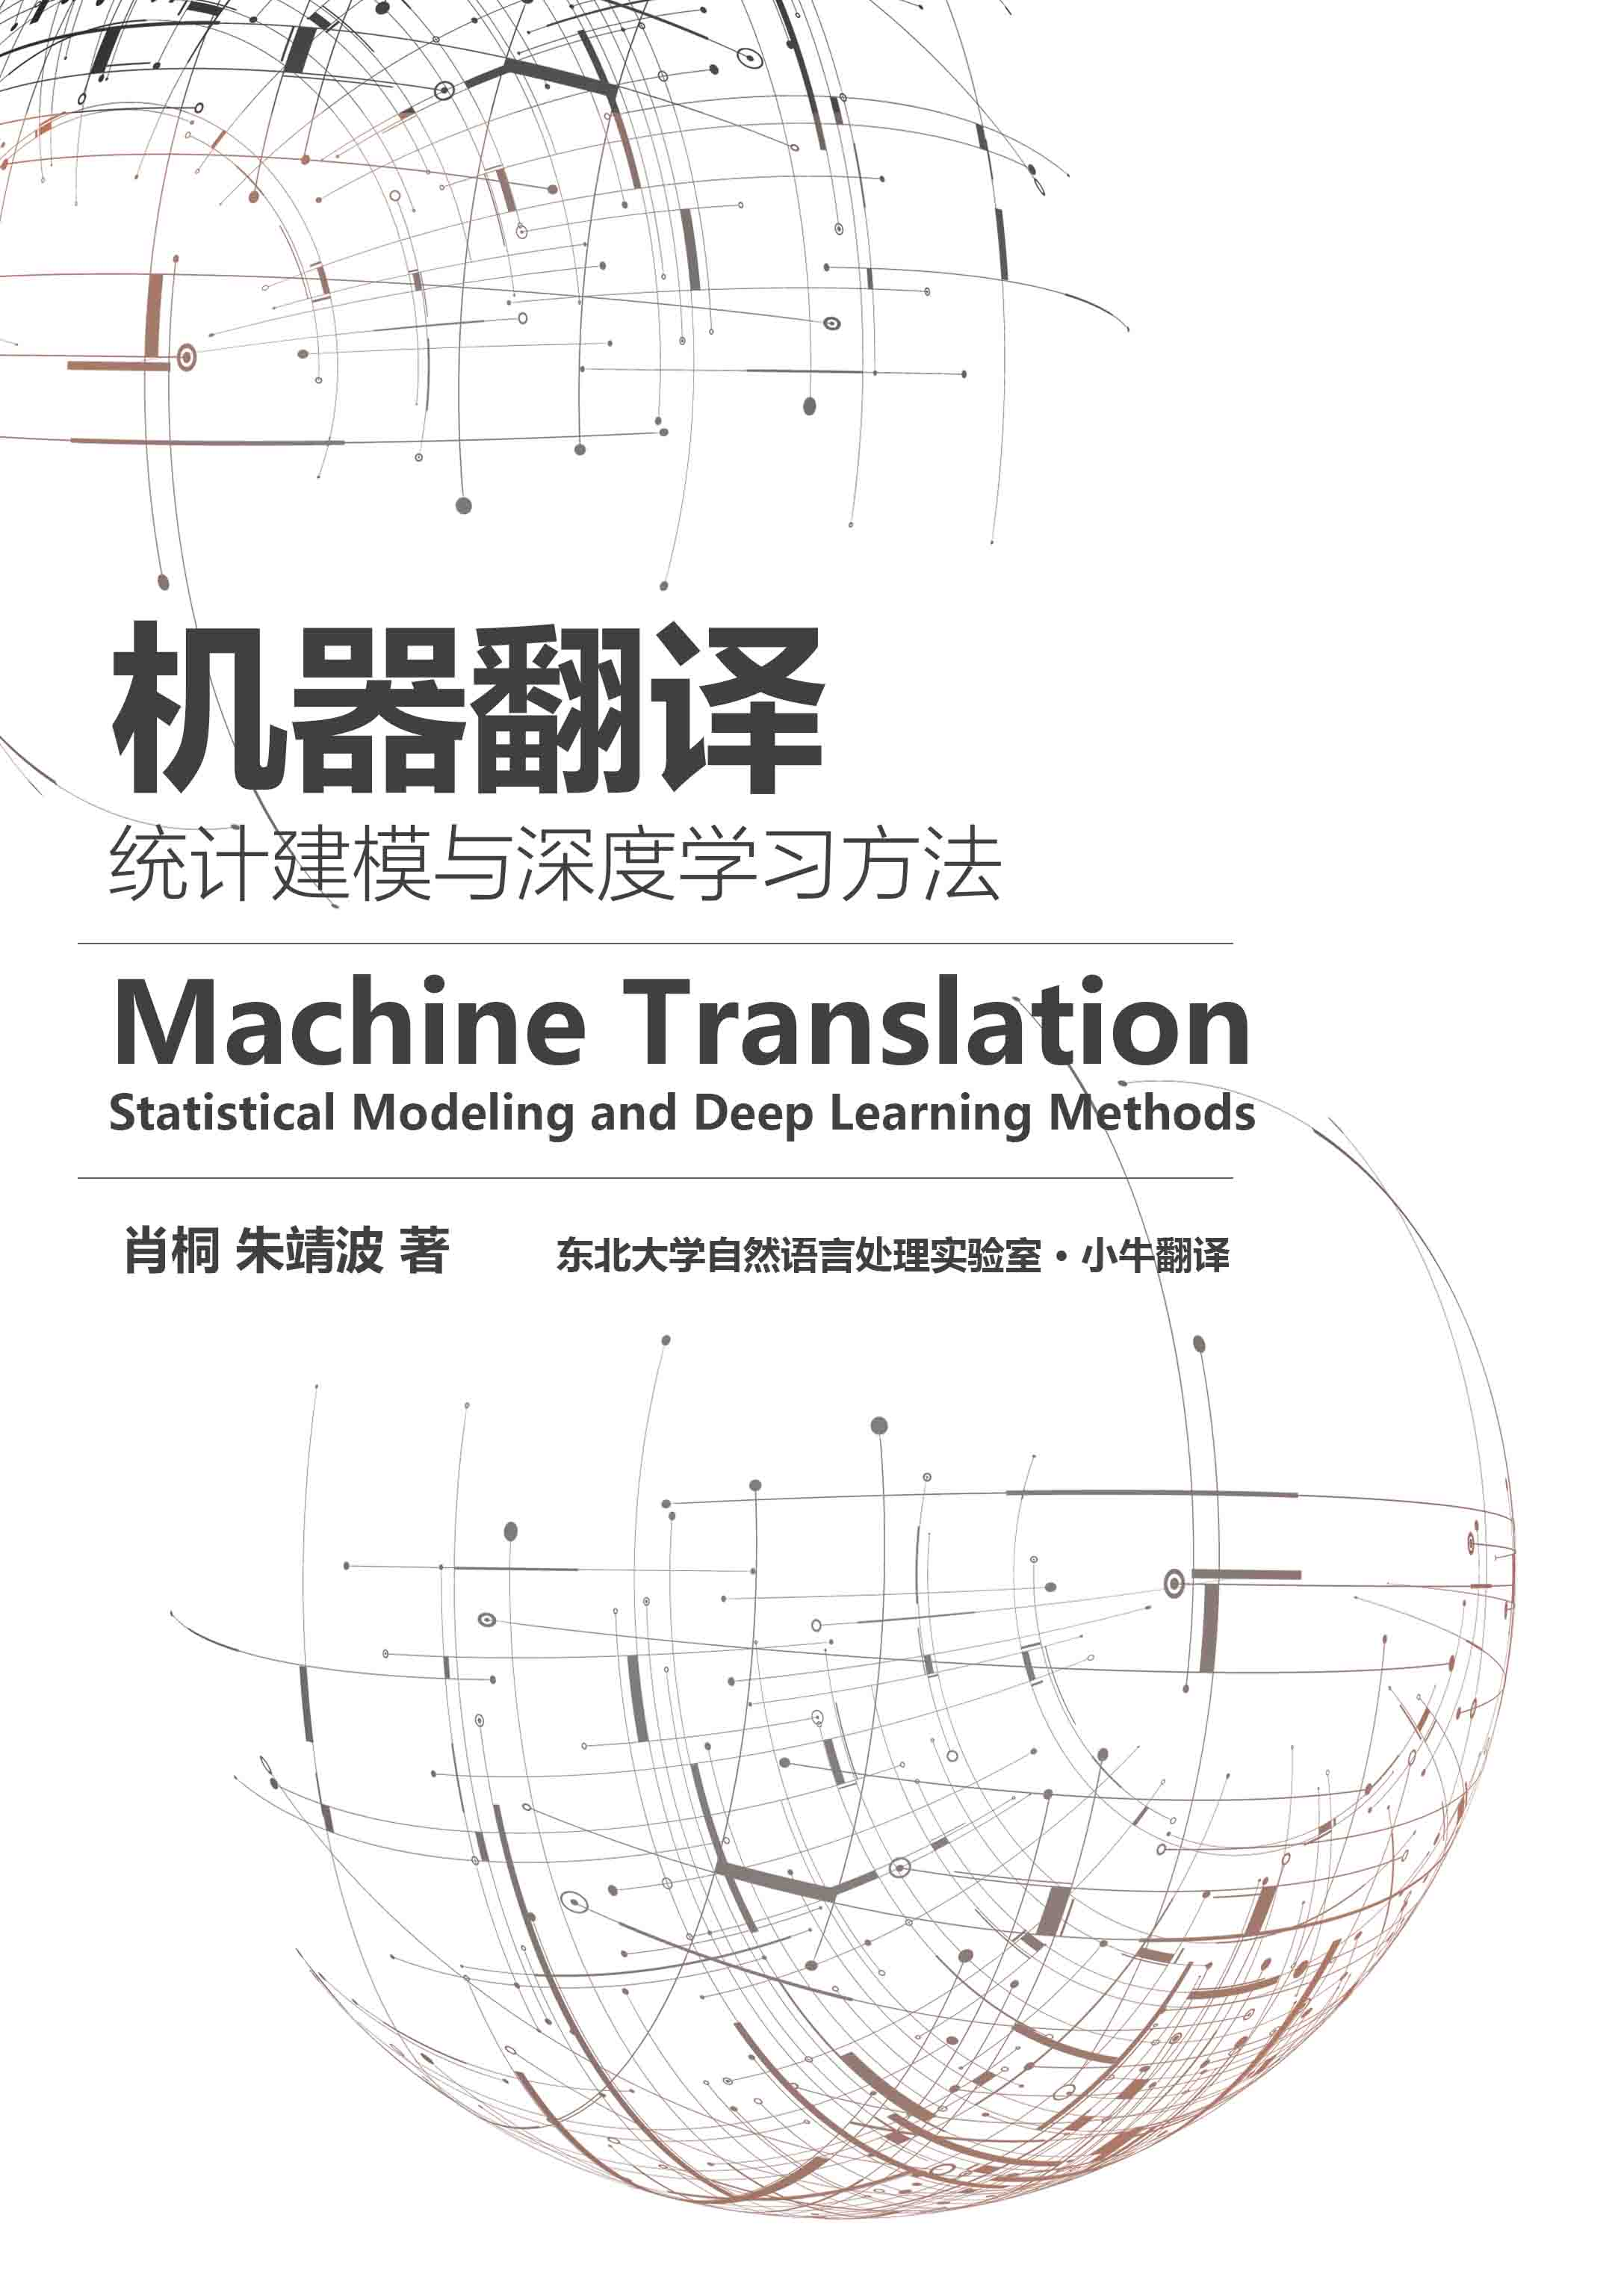
\includegraphics[width=\paperwidth,height=\paperheight]{fig-cover.jpg}};

\end{tikzpicture}
\vfill
\endgroup·

%----------------------------------------------------------------------------------------
%	COPYRIGHT PAGE
%----------------------------------------------------------------------------------------

\newpage
~\vfill
\thispagestyle{empty}

\noindent Copyright \copyright\ 2020 肖桐\ \ 朱靖波\\

\noindent \textsc{东北大学自然语言处理实验室\ $\cdot$\ 小牛翻译}\\

\noindent 顾问:姚天顺\ \ 王宝库\\

\noindent \textsc{\url{https://opensource.niutrans.com/mtbook/index.html}}\\
\noindent \textsc{\url{https://github.com/NiuTrans/MTBook}}\\

\noindent {\red{Licensed under the Creative Commons Attribution-NonCommercial 4.0 Unported License (the ``License''). You may not use this file except in compliance with the License. You may obtain a copy of the License at \url{http://creativecommons.org/licenses/by-nc/4.0}. Unless required by applicable law or agreed to in writing, software distributed under the License is distributed on an \textsc{``as is'' basis, without warranties or conditions of any kind}, either express or implied. See the License for the specific language governing permissions and limitations under the License.}}\\

\noindent \textit{\today}

%----------------------------------------------------------------------------------------
%	ACKNOWLEDGE PAGE
%----------------------------------------------------------------------------------------

\newpage
~\vfill
\thispagestyle{empty}

{\large
\noindent {\color{red} 在此感谢为本书做出贡献的小牛团队(部分)成员} \\

\noindent 曹润柘、曾信、孟霞、单韦乔、姜雨帆、王子扬、刘辉、许诺、李北、刘继强、张哲旸、周书含、周涛、张裕浩、李炎洋、林野、陈贺轩、刘晓倩、牛蕊、田丰宁、杜权、李垠桥、许晨、张裕浩、胡驰、冯凯、王泽洋、刘腾博、刘兴宇、徐萍、赵闯、高博、张春良、王会珍、张俐、杨木润、宁义明、李洋、秦浩、胡明涵 \\
}

%----------------------------------------------------------------------------------------
%	PREFACE PAGES
%----------------------------------------------------------------------------------------
\newpage
% !Mode:: "TeX:UTF-8"
% !TEX encoding = UTF-8 Unicode

%----------------------------------------------------------------------------------------
% 机器翻译:统计建模与深度学习方法
% Machine Translation: Statistical Modeling and Deep Learning Methods
%
% Copyright 2020
% 肖桐(xiaotong@mail.neu.edu.cn) 朱靖波 (zhujingbo@mail.neu.edu.cn)
%----------------------------------------------------------------------------------------

\renewcommand\figurename{图}

%----------------------------------------------------------------------------------------
%	PREFACE
%----------------------------------------------------------------------------------------

{\color{white} 空}
\vspace{0.5em}
\begin{center}
{\Huge \bfnew{导\ \ \ \ 读}}
\end{center}
\vspace{2em}

\begin{spacing}{1.18}

让计算机进行自然语言的翻译是人类长期的梦想,也是人工智能的终极目标之一。自上世纪九十年代起,机器翻译迈入了基于统计建模的时代,发展到今天,深度学习等机器学习方法已经在机器翻译中得到了大量的应用,取得了令人瞩目的进步。

在这个时代背景下,对机器翻译的模型、方法和实现技术进行深入了解是自然语言处理领域研究者和实践者所渴望的。本书全面回顾了近三十年内机器翻译的技术发展历程,并围绕统计建模和深度学习两个主题对机器翻译的技术方法进行了全面介绍。在写作中,笔者力求用朴实的语言和简洁的实例阐述机器翻译的基本模型和方法,同时对相关的技术前沿进行讨论。本书可以供计算机相关专业高年级本科生及研究生学习之用,也可以作为自然语言处理,特别是机器翻译领域相关研究人员的参考资料。

本书共分为七个章节,章节的顺序参考了机器翻译技术发展的时间脉络,同时兼顾了机器翻译知识体系的内在逻辑。各章节的主要内容包括:

\begin{itemize}
\vspace{0.5em}
\item 第一章:机器翻译简介
\vspace{0.5em}
\item 第二章:词法、语法及统计建模基础
\vspace{0.5em}
\item 第三章:基于词的机器翻译模型
\vspace{0.5em}
\item 第四章:基于短语和句法的机器翻译模型
\vspace{0.5em}
\item 第五章:人工神经网络和神经语言建模
\vspace{0.5em}
\item 第六章:神经机器翻译模型
\vspace{0.5em}
\item 第七章:神经机器翻译实战 \ \dash \ 参加一次比赛
\vspace{0.5em}
\end{itemize}

其中,第一章是对机器翻译的整体介绍。第二章和第五章是对统计建模和深度学习方法的介绍,分别建立了两个机器翻译范式的基础知识体系 \ \dash \ 统计机器翻译和神经机器翻译。统计机器翻译部分(第三、四章)涉及早期的基于单词的翻译模型,以及本世纪初流行的基于短语和句法的翻译模型。神经机器翻译(第六、七章)代表了当今机器翻译的前沿,内容主要涉及了基于端到端表示学习的机器翻译建模方法。特别地,第七章对一些最新的神经机器翻译方法进行了讨论,为相关科学问题的研究和实用系统的开发提供了可落地的思路。图\ref{fig:preface}展示了本书各个章节及核心概念之间的关系。

{\red 用最简单的方式阐述机器翻译的基本思想}是笔者所期望达到的目标。但是,书中不可避免会使用一些形式化定义和算法的抽象描述,因此,笔者尽所能通过图例进行解释(本书共320张插图)。不过,本书所包含的内容较为广泛,难免会有疏漏,望读者海涵,并指出不当之处。

%-------------------------------------------
\begin{figure}[htp]
\centering
\centering
% !Mode:: "TeX:UTF-8"
% !TEX encoding = UTF-8 Unicode

\begin{tikzpicture}

\tikzstyle{secnode} =[font=\scriptsize,minimum height=4.0em,minimum width=22em,draw,thick,fill=white,drop shadow]
\tikzstyle{conceptnode} =[font=\scriptsize,minimum height=1.5em,minimum width=5em]
\tikzstyle{conceptnodesmall} =[font=\scriptsize,minimum height=1.0em,minimum width=4.4em]

% section 1
\node [secnode,anchor=south west,minimum width=22.5em,red,fill=white] (sec1) at (0,0) {};
\node [anchor=north] (sec1label) at ([yshift=-0.2em]sec1.north) {\small{机器翻译简介}};
\node [anchor=north west,draw=red,thick,fill=white,rounded corners] (sec1title) at ([xshift=-0.3em,yshift=0.3em]sec1.north west) {{\footnotesize\bfnew{\color{red} 第一章}}};
\node [conceptnode,anchor=south west,fill=red!15,thin] (sec1box1) at ([xshift=0.5em,yshift=0.5em]sec1.south west) {\footnotesize{发展历史}};
\node [conceptnode,anchor=west,fill=red!15,thin] (sec1box2) at ([xshift=0.5em]sec1box1.east) {\footnotesize{评价方法}};
\node [conceptnode,anchor=west,fill=red!15,thin] (sec1box3) at ([xshift=0.5em]sec1box2.east) {\footnotesize{应用情况}};
\node [conceptnode,anchor=west,fill=red!15,thin] (sec1box4) at ([xshift=0.5em]sec1box3.east) {\footnotesize{系统\&数据}};


% section 2
\node [secnode,anchor=south,blue,fill=white] (sec2) at ([xshift=-6.5em,yshift=3em]sec1.north) {};
\node [anchor=north] (sec2label) at (sec2.north) {\small{词法、语法及统计建模基础}};
\node [anchor=north west,draw=blue,thick,fill=white,rounded corners] (sec2title) at ([xshift=-0.3em,yshift=0.3em]sec2.north west) {{\footnotesize\bfnew{\color{blue} 第二章}}};
\node [conceptnode,anchor=south west,fill=ublue!15,thin,minimum width=4em,align=left] (sec2box1) at ([xshift=0.5em,yshift=0.4em]sec2.south west) {\tiny{概率论与}\\\tiny{统计建模基础}};
\node [anchor=west,draw,dotted,thick,minimum height=2em,minimum width=16.6em,align=left] (sec2box2) at ([xshift=0.3em]sec2box1.east) {};
\node [conceptnodesmall,minimum width=5em,anchor=south west,fill=blue!15,thin] (sec2box3) at ([xshift=0.4em,yshift=0.3em]sec2box2.south west) {\scriptsize{中文分词}};
\node [conceptnodesmall,minimum width=5em,anchor=west,fill=blue!15,thin] (sec2box4) at ([xshift=0.4em]sec2box3.east) {\scriptsize{$n$元语法模型}};
\node [conceptnodesmall,minimum width=5em,anchor=west,fill=blue!15,thin] (sec2box5) at ([xshift=0.4em]sec2box4.east) {\scriptsize{句法分析}};


\draw [->,very thick] ([xshift=-1em,yshift=0.2em]sec1.north) .. controls +(north:2.5em) and +(south:2.5em) .. ([xshift=-3em,yshift=-0.2em]sec2.south);

% section 5
\node [secnode,anchor=south,orange,fill=white] (sec5) at ([xshift=7em,yshift=10em]sec1.north) {};
\node [anchor=north] (sec5label) at (sec5.north) {\small{人工神经网络和神经语言建模}};
\node [anchor=north west,draw=orange,thick,fill=white,rounded corners] (sec5title) at ([xshift=-0.3em,yshift=0.3em]sec5.north west) {{\footnotesize\bfnew{\color{orange} 第五章}}};
\node [conceptnode,minimum width=4em,anchor=south west,fill=orange!15,thin,align=left] (sec5box1) at ([xshift=0.5em,yshift=0.4em]sec5.south west) {\tiny{线性代数基础}\\\tiny{与感知机}};
\node [conceptnode,minimum width=4em,anchor=west,fill=orange!15,thin,align=left] (sec5box2) at ([xshift=0.2em]sec5box1.east) {\tiny{多层神经网络}\\\tiny{与实现方法}};
\node [conceptnode,minimum width=4em,anchor=west,fill=orange!15,thin,align=left] (sec5box3) at ([xshift=0.2em]sec5box2.east) {\tiny{模型训练}\\\tiny{(反向传播)}};
\node [conceptnode,minimum width=4em,anchor=west,fill=purple!15,thin,align=left] (sec5box4) at ([xshift=0.2em]sec5box3.east) {\tiny{神经语言模型}\\\tiny{(FNN等)}};
\node [conceptnode,minimum width=4em,anchor=west,fill=purple!15,thin,align=left] (sec5box5) at ([xshift=0.2em]sec5box4.east) {\tiny{表示学习与}\\\tiny{预训练模型}};
\node [draw,dotted,thick,inner sep=1pt] [fit = (sec5box4) (sec5box5)] (pretrainbox) {};


\draw [->,very thick] ([yshift=-9.8em]sec5.south) -- ([yshift=-0.2em]sec5.south);
\draw [->,thick,dotted] ([xshift=0.2em,yshift=1em]sec2.east) .. controls +(east:3em) and +(south:4em) .. ([xshift=3em,yshift=-0.0em]pretrainbox.south);

% section 3
\node [secnode,anchor=south,ugreen,fill=white] (sec3) at ([yshift=10em]sec2.north) {};
\node [anchor=north] (sec3label) at (sec3.north) {\small{基于词的机器翻译模型}};
\node [anchor=north west,draw=ugreen,thick,fill=white,rounded corners] (sec3title) at ([xshift=-0.3em,yshift=0.3em]sec3.north west) {{\footnotesize\bfnew{\color{ugreen} 第三章}}};
\node [conceptnode,minimum width=4em,anchor=south west,fill=ublue!15,thin,align=left] (sec3box1) at ([xshift=0.5em,yshift=0.4em]sec3.south west) {\tiny{机器翻译的统计}\\\tiny{描述(实例)}};
\node [conceptnode,minimum width=4em,anchor=west,fill=green!20,thin,align=left] (sec3box2) at ([xshift=0.2em]sec3box1.east) {\tiny{噪声信道模型}\\\tiny{与生成式模型}};
\node [conceptnode,minimum width=4em,anchor=west,fill=green!20,thin,align=left] (sec3box3) at ([xshift=0.2em]sec3box2.east) {\tiny{IBM模型、隐}\\\tiny{马尔可夫模型}};
\node [conceptnode,minimum width=4em,anchor=west,fill=green!20,thin,align=left] (sec3box4) at ([xshift=0.2em]sec3box3.east) {\tiny{\hspace{0.9em}参数学习}\\\tiny{=优化}};
\node [conceptnode,minimum width=3.8em,anchor=west,fill=green!20,thin,align=left,minimum height=2em,inner sep=2pt] (sec3box5) at ([xshift=0.2em]sec3box4.east) {\scriptsize{EM算法}};

\draw [->,very thick] ([yshift=0.2em,xshift=-3em]sec2.north) -- ([yshift=-0.2em,xshift=-3em]sec3.south);

% section 4
\node [secnode,anchor=south,ugreen,fill=white] (sec4) at ([yshift=3em]sec3.north) {};
\node [anchor=north] (sec4label) at (sec4.north) {\small{基于短语和句法的机器翻译模型}};
\node [anchor=north west,draw=ugreen,thick,fill=white,rounded corners] (sec4title) at ([xshift=-0.3em,yshift=0.3em]sec4.north west) {{\footnotesize\bfnew{\color{ugreen} 第四章}}};
\node [conceptnode,minimum width=4em,anchor=south west,fill=ublue!15,thin,align=left] (sec4box1) at ([xshift=0.5em,yshift=0.4em]sec4.south west) {\tiny{判别式模型与}\\\tiny{最小错误率训练}};
\node [conceptnode,minimum width=4em,anchor=west,fill=green!20,thin,align=left] (sec4box2) at ([xshift=0.2em]sec4box1.east) {\tiny{基于翻译推导}\\\tiny{的建模}};
\node [conceptnode,minimum width=4em,anchor=west,fill=green!20,thin,align=left] (sec4box3) at ([xshift=0.2em]sec4box2.east) {\tiny{短语及句法}\\\tiny{翻译规则抽取}};
\node [conceptnode,minimum width=4em,anchor=west,fill=green!20,thin,align=left,minimum height=2em,inner sep=2pt] (sec4box4) at ([xshift=0.2em]sec4box3.east) {\scriptsize{调序模型}};
\node [conceptnode,minimum width=3.8em,anchor=west,fill=green!20,thin,align=left,minimum height=2em,inner sep=2pt] (sec4box5) at ([xshift=0.2em]sec4box4.east) {\scriptsize{解码}};

\draw [->,very thick] ([yshift=0.2em,xshift=-3em]sec3.north) -- ([yshift=-0.2em,xshift=-3em]sec4.south);

% section 6
\node [secnode,anchor=south,purple,fill=white] (sec6) at ([yshift=19em]sec5.north) {};
\node [anchor=north] (sec6label) at (sec6.north) {\small{神经机器翻译模型}};
\node [anchor=north west,draw=purple,thick,fill=white,rounded corners] (sec6title) at ([xshift=-0.3em,yshift=0.3em]sec6.north west) {{\footnotesize\bfnew{\color{purple} 第六章}}};
\node [conceptnode,minimum width=4em,anchor=south west,fill=ublue!15,thin,align=left] (sec6box1) at ([xshift=0.5em,yshift=0.4em]sec6.south west) {\tiny{编码器-解码器}\\\tiny{框架}};
\node [conceptnode,minimum width=4em,anchor=west,fill=ublue!15,thin,align=left,minimum height=2em] (sec6box2) at ([xshift=0.2em]sec6box1.east) {\scriptsize{注意力机制}};
\node [conceptnode,minimum width=7.5em,anchor=west,fill=purple!15,thin,align=left] (sec6box3) at ([xshift=0.2em]sec6box2.east) {\tiny{基于RNN和Transformer}\\\tiny{的神经机器翻译建模}};
\node [conceptnode,minimum width=4em,anchor=west,fill=purple!15,thin,align=left,minimum height=2em] (sec6box4) at ([xshift=0.2em]sec6box3.east) {\scriptsize{训练与推断}};

\draw [->,very thick] ([yshift=0.2em]sec5.north) -- ([yshift=-0.2em]sec6.south);
\draw [->,very thick,dotted] ([yshift=0.2em,xshift=-2em]sec4.north) .. controls +(north:5.0em) and +(west:4em) .. ([xshift=-0.2em]sec6.west);
\draw [->,thick,dotted] ([xshift=3em,yshift=0.2em]pretrainbox.north) .. controls +(north:15em) and +(south:15em) .. ([xshift=0em,yshift=-0.0em]sec6box3.south);

% section 7
\node [secnode,anchor=south,purple,fill=white,minimum height=6.3em] (sec7) at ([yshift=3em]sec6.north) {};
\node [anchor=north] (sec7label) at (sec7.north) {\small{神经机器翻译实战}};
\node [anchor=north west,draw=purple,thick,fill=white,rounded corners] (sec7title) at ([xshift=-0.3em,yshift=0.3em]sec7.north west) {{\footnotesize\bfnew{\color{purple} 第七章}}};
\node [conceptnode,minimum width=4em,anchor=south west,fill=ublue!15,thin,align=left,minimum height=4.2em] (sec7box1) at ([xshift=0.5em,yshift=0.4em]sec7.south west) {\tiny{数据处理、}\\\tiny{子词切分}};

\node [anchor=north west,minimum width=5em,anchor=north west,fill=purple!15] (sec7box2) at ([xshift=0.5em,yshift=-0.2em]sec7box1.north east) {\tiny{正则化}};
\node [anchor=north west,minimum width=5em,anchor=north west,fill=purple!15] (sec7box3) at ([yshift=-0.1em]sec7box2.south west) {\tiny{增大模型容量}};
\node [anchor=north west,minimum width=5em,anchor=north west,fill=purple!15] (sec7box4) at ([yshift=-0.1em]sec7box3.south west) {\tiny{大批量训练}};

\node [anchor=north west,minimum width=5em,anchor=north west,fill=purple!15] (sec7box5) at ([xshift=0.6em]sec7box2.north east) {\tiny{推断优化}};
\node [anchor=north west,minimum width=5em,anchor=north west,fill=purple!15] (sec7box6) at ([yshift=-0.1em]sec7box5.south west) {\tiny{译文长度控制}};
\node [anchor=north west,minimum width=5em,anchor=north west,fill=purple!15] (sec7box7) at ([yshift=-0.1em]sec7box6.south west) {\tiny{多模型集成}};

\node [anchor=north west,minimum width=5em,anchor=north west,fill=purple!15] (sec7box8) at ([xshift=0.6em]sec7box5.north east) {\tiny{深层模型}};
\node [anchor=north west,minimum width=5em,anchor=north west,fill=purple!15] (sec7box9) at ([yshift=-0.1em]sec7box8.south west) {\tiny{知识精炼}};
\node [anchor=north west,minimum width=5em,anchor=north west,fill=purple!15] (sec7box10) at ([yshift=-0.1em]sec7box9.south west) {\tiny{单语数据使用}};

\node [draw,dotted,thick,inner sep=1pt] [fit = (sec7box2) (sec7box3) (sec7box4)] (trainbox) {};
\node [draw,dotted,thick,inner sep=1pt] [fit = (sec7box5) (sec7box6) (sec7box7)] (inferencebox) {};
\node [draw,dotted,thick,inner sep=1pt] [fit = (sec7box8) (sec7box9) (sec7box10)] (advancedbox) {};

\draw [->,very thick] ([yshift=0.2em]sec6.north) -- ([yshift=-0.2em]sec7.south);
\draw [->,very thick,dotted] ([yshift=0.2em,xshift=-3em]sec4.north) .. controls +(north:7.0em) and +(west:6em) .. ([xshift=-0.2em]sec7.west);

%caption
\node [anchor=north] (caption) at ([xshift=0.4em,yshift=-1em]sec1.south) {\footnotesize{本书各章节及核心概念关系图}};


\end{tikzpicture}

\end{figure}
%-------------------------------------------

\end{spacing}










%----------------------------------------------------------------------------------------
%	TABLE OF CONTENTS
%----------------------------------------------------------------------------------------
%\usechapterimagefalse % If you don't want to include a chapter image, use this to toggle images off - it can be enabled later with \usechapterimagetrue
\chapterimage{fig-NEU-1.jpg} % Image of the content page
\pagestyle{empty} % Disable headers and footers for the following pages
\tableofcontents % Show contents
\cleardoublepage % Place the first page of each chapter on odd pages
\pagestyle{fancy} % Enable headers and footers


%----------------------------------------------------------------------------------------
%	CHAPTERS
%----------------------------------------------------------------------------------------

% !Mode:: "TeX:UTF-8"
% !TEX encoding = UTF-8 Unicode

%----------------------------------------------------------------------------------------
% 机器翻译:统计建模与深度学习方法
% Machine Translation: Statistical Modeling and Deep Learning Methods
%
% Copyright 2020
% 肖桐(xiaotong@mail.neu.edu.cn) 朱靖波 (zhujingbo@mail.neu.edu.cn)
%----------------------------------------------------------------------------------------

%----------------------------------------------------------------------------------------
%    CONFIGURATIONS
%----------------------------------------------------------------------------------------

\part{机器翻译基础}
\renewcommand\figurename{图}%将figure改为图
\renewcommand\tablename{表}%将figure改为图
\chapterimage{fig-NEU-2.jpg} % Chapter heading image

%----------------------------------------------------------------------------------------
%	CHAPTER 1
%----------------------------------------------------------------------------------------

\chapter{机器翻译简介}

%----------------------------------------------------------------------------------------
%    NEW SECTION
%----------------------------------------------------------------------------------------

\section{机器翻译的概念}

\parinterval 从广义上来讲,``翻译''是指把一个事物转化为另一个事物的过程。这个概念多使用在对序列的转化上,比如,计算机程序的编译、自然语言文字翻译、蛋白质生物合成等。在程序编译中,高级语言编写的程序经过一系列的处理后转化为可执行的目标程序,这是一种从高级程序语言到低级程序语言的``翻译''。在人类语言的翻译中,一种语言文字通过人脑转化为另一种语言表达,这是一种自然语言的``翻译''。在蛋白质合成的第一步,RNA分子序列转化为特定的氨基酸序列,这是一种生物学遗传信息的``翻译''。甚至说给上联对出下联、给一幅图片写出图片的主题等都可以被看作是``翻译''的过程。
\vspace{0.5em}

%----------------------------------------------
\begin{figure}[htp]
    \centering
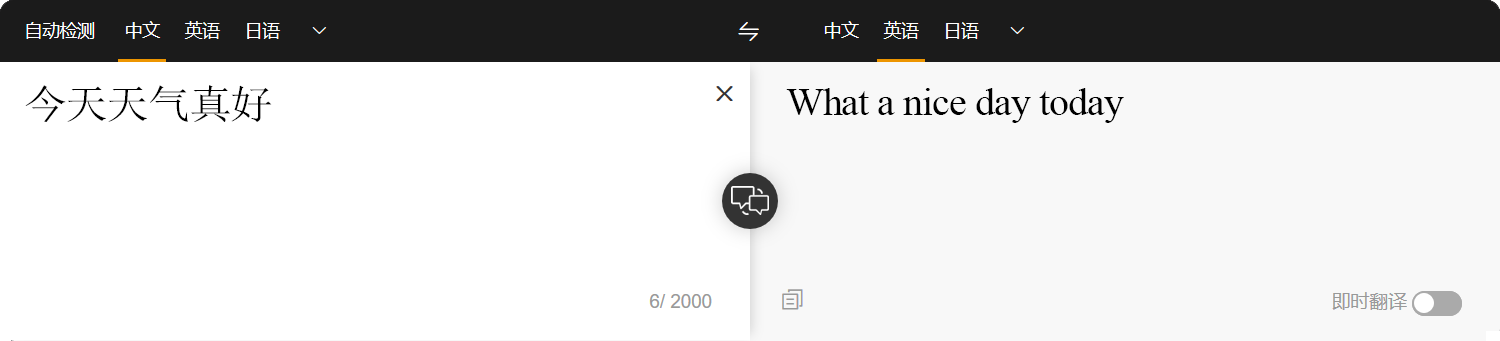
\includegraphics[scale=0.2]{./Chapter1/Figures/figure-zh_en-example.png}
    \caption{通过计算机将中文翻译为英文}
    \label{fig:1-1}
\end{figure}
%----------------------------------------------

\parinterval 这里更加关注人类语言之间的翻译问题,即自然语言的翻译。如图\ref{fig:1-1}所示,通过计算机可以将一段中文文字自动转化为英文文字,中文被称为{\small\bfnew{源语言}}\index{源语言}(Source Language)\index{Source Language},英文被称为{\small\bfnew{目标语言}}\index{目标语言}(Target Language)\index{Target Language}。

\parinterval 一直以来,文字的翻译往往是由人工完成。让计算机像人一样进行翻译似乎还是电影中的桥段,因为人们很难想象语言的多样性和复杂性可以用计算机语言进行描述。但是时至今日,人工智能技术的发展已经大大超越了人类传统的认知,用计算机进行自动翻译也不再是一种梦想,它已经深入到人们生活的很多方面,并发挥着重要作用。而这种由计算机进行自动翻译的过程也被称作{\small\bfnew{机器翻译}}\index{机器翻译}(Machine Translation)\index{Machine Translation}。类似地,自动翻译、智能翻译、多语言自动转换等概念也是指同样的事情。如果将今天的机器翻译和人工翻译进行对比,可以发现机器翻译系统所生成的译文还并不完美,甚至有时翻译质量非常差,但是它的生成速度快且成本低廉,更为重要的是机器翻译系统可以从大量数据中不断学习和进化。

\parinterval 人工翻译尽管精度很高,但是费时费力。当需要翻译大量的文本且精度要求不那么高时,比如海量数据的浏览型任务,机器翻译的优势就体现出来了。对于人工作业无法完成的事情,使用机器翻译可能只需花费几个小时甚至几分钟就能完成。这就类似于拿着锄头耕地种庄稼和使用现代化机器作业之间的区别。

\parinterval 实现机器翻译往往需要多个学科知识的融合,如数学、语言学、计算机科学、心理学等等。而最终呈现给使用者的是一套软件系统\ \dash\ 机器翻译系统。通俗来讲,机器翻译系统就是一个可以在计算机上运行的软件工具,与人们使用的其他软件一样,只不过机器翻译系统是由``不可见的程序''组成。虽然这个系统非常复杂,但是呈现出来的展示形式却很简单,比如输入是待翻译的句子或文本,输出是译文句子或文本。

%----------------------------------------------
\begin{figure}[htp]
    \centering
\input{./Chapter1/Figures/figure-required-parts-of-mt}
    \caption{机器翻译系统的组成}
    \label{fig:1-2}
\end{figure}
%-------------------------------------------

\parinterval 用机器进行翻译的想法可以追溯到电子计算机产生之前,发展过程中也经历了多个范式的变迁,现代机器翻译系统大多是基于数据驱动的方法\ \dash\ 从数据中自动学习翻译知识,并运用这些知识对新的文本进行翻译。如图\ref{fig:1-2}所示,机器翻译系统通常由两部分组成:

\begin{itemize}
\vspace{0.5em}
\item {\small\bfnew{资源}}:如果把机器翻译系统比作一辆汽车,资源就好比是可以使汽车运行的``汽油'',它包括很多内容,如翻译规则、双(单)语数据、知识库等翻译知识,且这些``知识''都是计算机可读的。值得一提的是,如果没有翻译资源的支持,任何机器翻译系统都无法运行起来。
\vspace{0.5em}
\item {\small\bfnew{系统}}:机器翻译算法的程序实现被称作系统,也就是机器翻译研究人员开发的软件。无论是翻译规则、翻译模板还是统计模型中的参数都需要通过机器翻译系统进行读取和使用。
\vspace{0.5em}
\end{itemize}

\parinterval 构建一个强大的机器翻译系统需要``资源''和``系统''两方面共同作用。在资源方面,随着语料库语言学的发展,已经有大量高质量的双语和单语数据(称为语料)被整理并且电子化存储,研发机器翻译系统所需要的语料基础已经具备。特别是像英语、汉语等世界主流语种,相关语料资源已经非常丰富,这也大大加速了相关研究的进展。当然,对于一些稀缺资源语种或者特殊的领域,语料库仍然匮乏,但是这些并不影响机器翻译领域整体的发展速度。在现有语料库的基础上,很多研究者可以把精力集中在``系统''上。但是,机器翻译并非易事,有以下几方面挑战:

\begin{itemize}
\vspace{0.5em}
\item {\small\bfnew{自然语言翻译问题的复杂性极高}}。语言是人类进化的最高成就之一,自然语言具有高度的概括性、灵活性、多样性,这些都很难用几个简单的模型和算法进行描述。因此,翻译问题的数学建模和计算机程序实现难度很大。虽然近几年AlphaGo等人工智能系统在围棋等领域取得了令人瞩目的成绩,但是,相比翻译来说,围棋等棋类任务仍然``简单''。正如不同人对同一句话的理解不尽相同,一个句子往往不存在绝对的标准译文,其潜在的译文几乎是不可穷尽的。甚至人类译员在翻译一个句子、一个单词的时候,都要考虑整个篇章的上下文语境。这些难点都不是传统棋类任务所具有的。
\vspace{0.5em}
\item {\small\bfnew{计算机的``理解''与人类的``理解''存在鸿沟}}。人类一直希望把自己翻译时所使用的知识描述出来,并用计算机程序进行实现,例如早期基于规则的机器翻译方法就源自这个思想。但是,经过实践发现,人和计算机在``理解''自然语言上存在着明显差异。首先,人类的语言能力是经过长时间在多种外部环境因素共同作用下形成的,这种能力很难直接准确地表达。况且人类的语言知识本身就很难描述,更不用说让计算机来理解;其次,人和机器翻译系统理解语言的目的不一样。人理解和使用语言是为了进行生活和工作,而机器翻译系统更多的是为了对某些数学上定义的目标函数进行优化。也就是说,机器翻译系统关注的是翻译这个单一目标,而并不是像人一样进行复杂的活动;此外,人和计算机的运行方式有着本质区别。人类语言能力的生物学机理与机器翻译系统所使用的计算模型本质上是不同的,机器翻译系统使用的是其自身能够理解的``知识'',比如,统计学上的词语表示。这种``知识''并不需要人来理解,当然从系统开发的角度,计算机也并不需要理解人是如何思考的。
\vspace{0.5em}
\item {\small\bfnew{单一的方法无法解决多样的翻译问题}}。首先,语种的多样性会导致任意两种语言之间的翻译实际上都是不同的翻译任务。比如,世界上存在的语言多达几千种,如果选择任意两种语言进行互译就产生上百万种翻译方向。虽然已经有研究者尝试用同一个框架甚至同一个翻译系统进行全语种的翻译,但是这类系统离真正可用还有很远的距离;其次,不同的领域,不同的应用场景对翻译也有不同的需求。比如,文学作品的翻译和新闻的翻译就有不同、口译和笔译也有不同,类似的情况不胜枚举。机器翻译要适用于多样的需求,这些又进一步增加了计算机建模的难度;再次,对于机器翻译来说,充足的高质量数据是必要的,但是不同语种、不同领域、不同应用场景所拥有的数据量有明显差异,甚至很多语种几乎没有可用的数据,这时开发机器翻译系统的难度可想而知。值得注意的是,现在的机器翻译还无法像人类一样在学习少量样例的情况下进行举一反三,因此数据稀缺情况下的机器翻译也给研究者带来了很大的挑战。
\vspace{0.5em}
\end{itemize}


\parinterval 显然,实现机器翻译并不简单,甚至有人把机器翻译看作是实现人工智能的终极目标。幸运的是,今天的机器翻译无论从技术方法上还是从应用上都有了巨大的飞跃,很多问题在不断被求解。如果你看到过十年前机器翻译的结果,再对比今天的结果,一定会感叹翻译质量的今非昔比,很多译文已经非常准确且流畅。从当今机器翻译的前沿技术看,近三十年机器翻译的进步更多的得益于基于数据驱动方法和统计建模方法的使用。特别是近些年深度学习等基于表示学习的端到端方法使得机器翻译的水平达到了新高度。因此,本书将会对基于统计建模和深度学习方法的机器翻译模型、方法和系统实现进行全面介绍和分析,希望这些内容可以对相关内容的学习和科研工作提供参考。

%----------------------------------------------------------------------------------------
%    NEW SECTION
%----------------------------------------------------------------------------------------

\sectionnewpage
\section{机器翻译简史}

\parinterval 虽然翻译这个概念在人类历史中已经存在了上千年,但机器翻译发展至今只有七十余年的历史。纵观机器翻译的发展,历程曲折又耐人寻味,可以说了解机器翻译的历史对我们深入理解相关技术方法会有很好的启发,甚至对我们了解整个自然语言处理领域的发展也有启示作用。

%----------------------------------------------------------------------------------------
%    NEW SUB-SECTION
%----------------------------------------------------------------------------------------

\subsection{人工翻译}

\parinterval 人类形成语言文字的过程中逐渐形成了翻译的概念。一个著名的标志性证据是罗塞塔石碑(Rosetta Stone),如图\ref{fig:1-3}所示。这个石碑制作于公元前196年,据说是可供考证的最久远的记载平行文字的历史遗迹。石碑由上至下刻有同一段埃及国王诏书的三种语言版本,最上面是古埃及象形文,中间是埃及草书,最下面是古希腊文。可以明显看出石碑上中下雕刻的文字的纹理是不同的。尽管用不同的语言文字描述同一件事在今天看来很常见,但是这在生产力低下的两千年前是很罕见的。很多人认为罗塞塔石碑是标志翻译或人工翻译的一个起点。目前罗塞塔石碑保存于大英博物馆,并成为该馆最具代表性的镇馆之宝之一。

%----------------------------------------------
\begin{figure}[htp]
    \centering
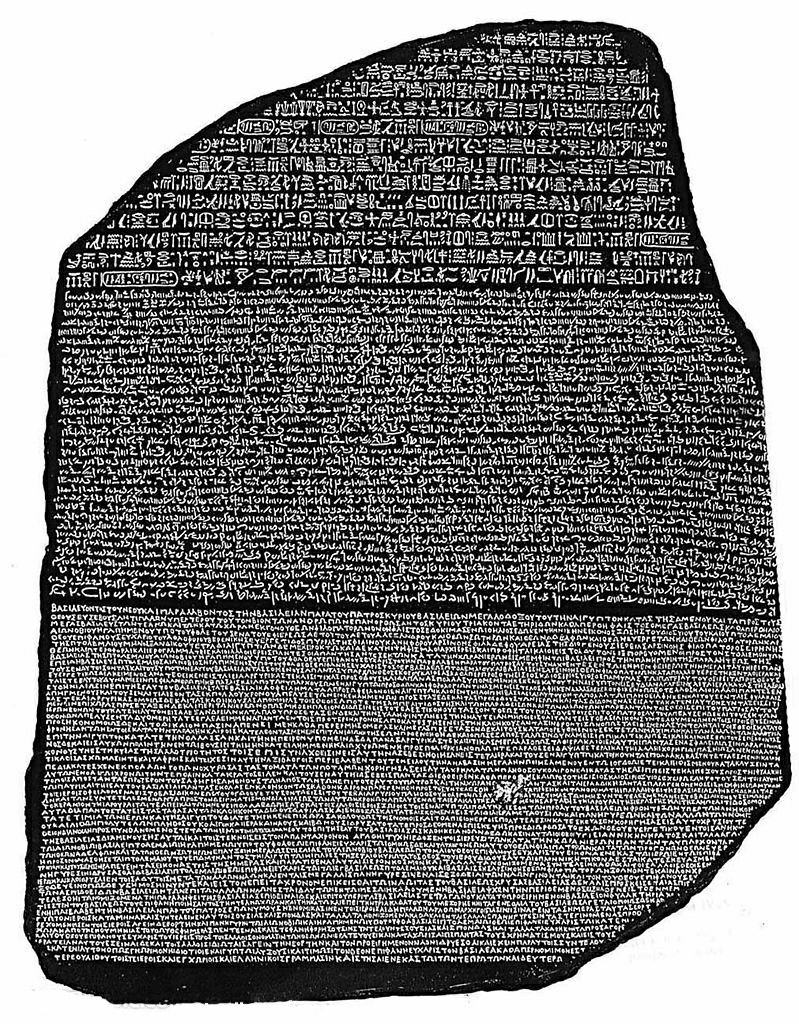
\includegraphics[scale=0.20]{./Chapter1/Figures/figure-rosetta-stone.jpg}
    \caption{罗塞塔石碑}
    \label{fig:1-3}
\end{figure}
%------------------------------------------

\parinterval 随后,更多的翻译工作在文化和知识传播中开展。其中一个典型代表是宗教文献的翻译。在人类的历史长河中,宗教是人类意识形态的一个重要载体。为了宣传教义,人们编写了大量的宗教文献。在西方,一项最早被记录的翻译活动是将旧约圣经(希伯来文及埃兰文)翻译为希腊文版本。迄今为止人类历史上翻译版本最多的书就是圣经。在中国唐代,有一位世界性的重量级文化人物\ \dash \ 玄奘,他不仅是佛学家、旅行家,还是翻译家。玄奘西行求法归来后把全部的心血和智慧奉献给了译经事业,在助手们的帮助下,共翻译佛教经论74部,1335卷,每卷万字左右,合计1335万字,占去整个唐代译经总数的一半以上,树立了我国古代翻译思想的光辉典范。

\parinterval 翻译在人类历史长河中起到了重要的作用。一方面,由于语言文字、文化和地理位置的差异性,使得翻译成为一个重要的需求;另一方面,翻译也加速了不同文明的融会贯通,促进了世界的发展。今天,翻译已经成为重要的行业之一,包括各个高校也都设立了翻译及相关专业,相关人才不断涌现。据《2019年中国语言服务行业发展报告》统计:全球语言服务产值预计将首次接近500亿美元;中国涉及语言服务的在营企业360,000余家,语言服务为主营业务的在营企业近万家,总产值超过300亿元,年增长3\%以上;全国开设外语类专业的高校数量多达上千所,其中设立有翻译硕士(MTI)和翻译本科(BTI)专业的院校分别有250余所和280余所,MTI累计招生数达6万余人\cite{赵军峰2019深化改革}。当然,面对着巨大的需求,如何使用机器辅助翻译等技术手段提高人工翻译效率,也是人工翻译和机器翻译领域需要共同探索的方向。

%----------------------------------------------------------------------------------------
%    NEW SUB-SECTION
%----------------------------------------------------------------------------------------

\subsection{机器翻译的萌芽}

\parinterval 人工翻译已经存在了上千年,而机器翻译又起源于什么时候呢?机器翻译跌宕起伏的发展史可以分为萌芽期、受挫期、快速成长期和爆发期四个阶段。

%----------------------------------------------
\begin{figure}[htp]
    \centering
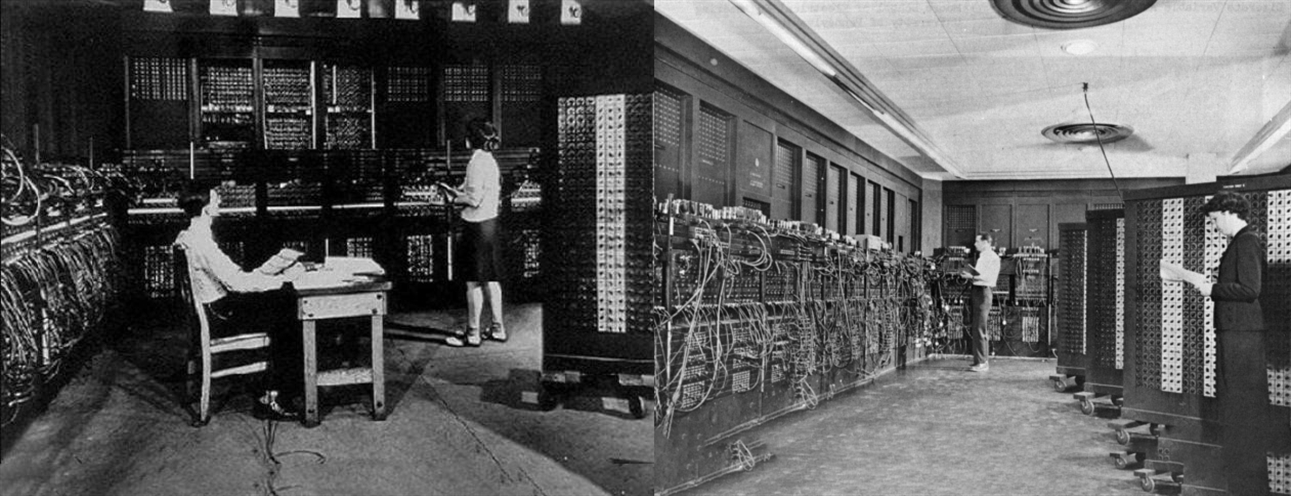
\includegraphics[scale=0.25]{./Chapter1/Figures/figure-eniac.jpg}
    \caption{世界上第一台通用电子数字计算机``埃尼阿克''(ENIAC)}
    \label{fig:1-4}
\end{figure}
%-------------------------------------------

\parinterval 世界上第一台通用电子数字计算机在1946年研制成功(图\ref{fig:1-4}\footnote{\url{https://baike.baidu.com/item/ENIAC}})。但在上世纪30年代使用计算模型进行自动翻译的思想就开始萌芽,当时法国科学家G.\ B.\ Artsouni提出了用机器来进行翻译的想法。

\parinterval 第二次世界大战使得数学和密码学相当发达,由于战争的需要,在那个时代消息传递变的更为隐秘,对文字进行加密和解密成为重要的军事需求。因此,有人提出是否能用密码学的技术或方法解决人类语言的翻译任务,比如把汉语看成英语的一个加密文本,汉语翻译成英语就类似于解密的过程。当然这只是最初的想法。第一次提出机器翻译这个概念是在1949年,当时W. Weaver撰写了一篇名为《翻译》的备忘录,正式开创了机器翻译(Machine Translation)的概念,这个概念一直沿用至今。当然,在那个年代进行机器翻译研究还有很多条件不具备,包括使用加密解密技术进行自动翻译的很多尝试很快也被验证是不可行的。不过,这些早期的探索为后来机器翻译的发展提供了思想的火种。

%----------------------------------------------------------------------------------------
%    NEW SUB-SECTION
%----------------------------------------------------------------------------------------

\subsection{机器翻译的受挫}

\parinterval 随着电子计算机的发展,研究者开始尝试使用计算机来进行自动的翻译。但是事情并不总是一帆风顺,怀疑论者对机器翻译一直存有质疑,并很容易找出一些机器翻译无法解决的问题。自然地,人们也期望能够客观地评估一下机器翻译的可行性。当时美国基金资助组织委任自动语言处理咨询会承担了这项任务。

\parinterval 经过近两年的调查与分析,该委员会于1966年11月公布了一个题为《语言与机器》的报告(图\ref{fig:1-5}),即ALPAC报告。该报告全面否定了机器翻译的可行性,为机器翻译的研究泼了一盆冷水。

\parinterval 随后美国政府终止了对机器翻译研究的支持,这导致整个产业界和学术界对机器翻译都开始回避。大家觉得机器翻译像伪科学,无论是发表论文还是申请项目都很难得到支持。没有了政府的支持,企业也无法进行大规模投入,机器翻译的研究就此受挫。

\parinterval 从历史上看,包括机器翻译在内很多人工智能领域在那个年代并不受``待见'',其主要原因在于当时的技术水平还比较低,而大家又对机器翻译等技术的期望过高。最后发现,当时的机器翻译水平无法满足实际需要,因此转而排斥它。但是,也正是这一盆冷水,让人们可以更加冷静的思考机器翻译的发展方向,为后来的爆发蓄力。

%----------------------------------------------
\begin{figure}[htp]
    \centering
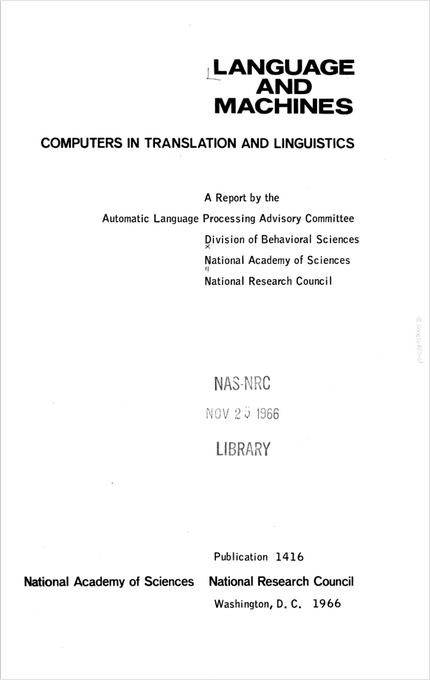
\includegraphics[scale=0.65]{./Chapter1/Figures/figure-report.jpg}
    \caption{ALPAC报告}
    \label{fig:1-5}
\end{figure}
%-------------------------------------------

%----------------------------------------------------------------------------------------
%    NEW SUB-SECTION
%----------------------------------------------------------------------------------------

\subsection{机器翻译的快速成长}

\parinterval 事物发展都是螺旋式上升的,机器翻译也是一样。上世纪70年代中后期,特别是80年代到90年代初,国家之间往来日益密切,而不同语言之间形成的交流障碍愈发严重,传统的人工作业方式已经远远不能满足需求。与此同时,语料库语言学的发展也为机器翻译提供了新的思路。其中,随着传统纸质文字资料不断电子化,计算机可读的语料越来越多,这使得人们可以用计算机对语言规律进行统计分析。另一方面,随着可用数据越来越多,用数学模型描述这些数据中的规律并进行推理逐渐成为可能。这也衍生出一类数学建模方法\ \dash\ {\small\bfnew{数据驱动}}\index{数据驱动}(Data-Driven)\index{Data-Driven}的方法。这类方法也成为了随后出现的统计机器翻译的基础。

传统的机器翻译方法,都需要人来书写规则,虽然对少部分句子具有较高的翻译精度,但这类方法对翻译现象的覆盖度有限,而且对规则或者模板中的噪声非常敏感,系统健壮性差。而基于数据驱动的方法不依赖于人写的规则,机器翻译的建模、训练和推断都可以自动地从数据中学习。这使得整个机器翻译的范式发生了翻天覆地的变化,比如,基于实例的方法和统计机器翻译就是在此期间兴起的。此外,这样的方法使得机器翻译系统的开发代价大大地降低。从上世纪90年代到本世纪初,统计机器翻译发展迅猛,很快成为了当时机器翻译研究与应用的代表性方法。一个标志性的事件是谷歌推出了一个在线的免费自动翻译服务,也就是大家熟知的谷歌翻译。这使得机器翻译这种``高大上''的技术快速进入人们的生活,而不再是束之高阁的科研想法。随着机器翻译不断走向实用,机器翻译的应用也越来越多,这反过来进一步促进了机器翻译的研究进程。比如,在2005-2015年间,统计机器翻译这个主题几乎统治了ACL等自然语言处理相关方向顶级会议的论文,可见其在当时的影响力。

%----------------------------------------------------------------------------------------
%    NEW SUB-SECTION
%----------------------------------------------------------------------------------------

\subsection{机器翻译的爆发}

\parinterval 2005年拉开了统计机器翻译发展十年黄金时期的序幕。在这一时期,各种基于统计机器翻译模型层出不穷,经典的基于短语的模型和基于句法的模型也先后被提出。在2013年以后,机器学习的进步带来了机器翻译技术的进一步提升。特别是基于神经网络的深度学习方法在机器视觉、语音识别中被成功应用,带来性能的飞跃式提升。很快,相关模型和方法也被用于机器翻译。对于机器翻译来说,深度学习的成功也是一种必然,原因如下:

\begin{itemize}
\vspace{0.5em}
\item 第一,端到端学习不依赖于过多的先验假设。在统计机器翻译时代,模型设计或多或少会对翻译的过程进行假设,称为隐藏结构假设。比如基于短语的模型假设:源语言和目标语言都会被切分成短语序列,这些短语之间存在某种对齐关系。这种假设既有优点也有缺点:一方面,该假设有助于模型融入人类的先验知识,比如假设中的短语就借鉴了语言学相关的概念;另一方面,假设越多模型受到的限制也越多。如果假设是正确的,模型可以很好地描述问题。但如果假设错误,那么模型就可能产生偏差。深度学习不依赖于先验知识,也不需要手工设计特征,模型直接从输入和输出的映射上进行学习(端到端学习),这样也在一定程度上避免了隐藏结构假设造成的偏差。
\vspace{0.5em}
\item 第二,神经网络的连续空间模型有更强的表示能力。机器翻译中的一个基本问题是:如何表示一个句子?统计机器翻译把句子的生成过程看作是短语或者规则的推导,这本质上是一个离散空间上的符号系统。深度学习把传统的基于离散化的表示变成了连续空间的表示。比如,用实数空间的分布式表示代替了离散化的词语表示,而整个句子可以被描述为一个实数向量。这使得翻译问题可以在连续空间上描述,进而大大缓解了传统离散空间模型维度灾难等问题。更重要的是,连续空间模型可以用梯度下降等方法进行优化,具有很好的数学性质并且易于实现。
\vspace{0.5em}
\item 第三,深度网络学习算法的发展和GPU(Graphics Processing Unit)等并行计算设备为训练神经网络提供了可能。早期的基于神经网络的方法一直没有在机器翻译甚至自然语言处理领域得到大规模应用,其中一个重要的原因是这类方法需要大量的浮点运算,而且以前计算机的计算能力无法达到这个要求。随着GPU等并行计算设备的进步,训练大规模神经网络也变为了可能。现在已经可以在几亿、几十亿,甚至上百亿句对上训练机器翻译系统,系统研发的周期越来越短,进展日新月异。
\vspace{0.5em}
\end{itemize}

\parinterval 今天,神经机器翻译已经成为新的范式,大有全面替代统计机器翻译之势。比如,从世界上著名的机器翻译比赛WMT和CCMT中就可以看出这个趋势。如图\ref{fig:1-6}所示,其中左图是WMT\ 19全球机器翻译比赛的参赛队伍的截图,这些参赛队伍基本上都在使用深度学习完成机器翻译的建模。而在WMT\ 19各个项目夺冠系统中(\ref{fig:1-6}右图),神经机器翻译也几乎一统天下。

\parinterval 值得一提的是,近些年神经机器翻译的快速发展也得益于产业界的关注。各大互联网企业和机器翻译技术研发机构都对神经机器翻译的模型和实践方法给予了很大贡献。比如,谷歌、微软、百度、搜狗、金山、腾讯、阿里、有道、讯飞、小牛翻译等企业凭借自身人才和基础设施方面的优势,先后推出了以神经机器翻译为内核的产品及服务,相关技术方法已经在大规模应用中得到验证,大大推动了机器翻译的产业化进程,而且这种趋势在不断加强,机器翻译的前景也更加宽广。

%----------------------------------------------
\begin{figure}[htp]
    \centering
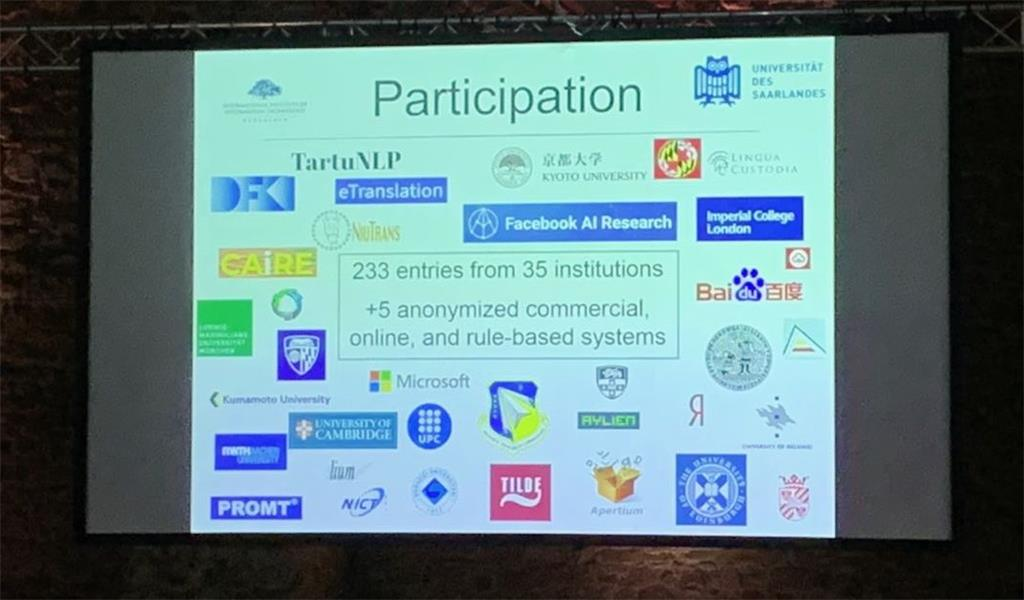
\includegraphics[scale=0.3]{./Chapter1/Figures/figure-wmt-participation.jpg}
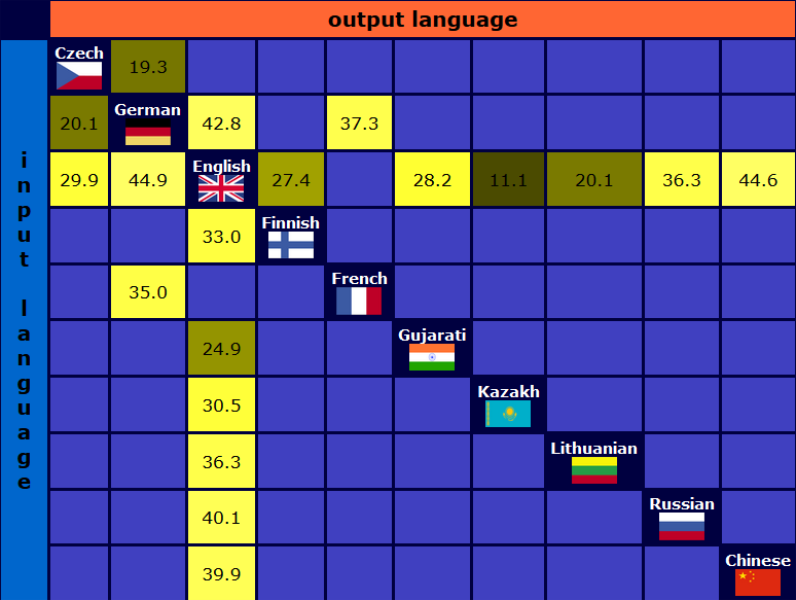
\includegraphics[scale=0.3]{./Chapter1/Figures/figure-wmt-bestresults.jpg}
\setlength{\belowcaptionskip}{-1.5em}
    \caption{国际机器翻译大赛(左:WMT\ 19参赛队伍;右:WMT\ 19各项目的最好分数结果)}
    \label{fig:1-6}
\end{figure}
%-------------------------------------------

%----------------------------------------------------------------------------------------
%    NEW SECTION
%----------------------------------------------------------------------------------------

\sectionnewpage
\section{机器翻译现状}
%%%%%%%%%%%%%%%%%%%%%%%%%%%%%%%%%%%%%%%%%%%%%%%%%%%%%%%%%%%%%%%%%%%%%%%%%%%%
\parinterval 机器翻译技术发展到今天已经过无数次迭代,技术范式也经过若干次更替,近些年机器翻译的应用也如雨后春笋。但是大家都很好奇今天的机器翻译的质量究竟如何呢?乐观地说,在受限条件下,机器翻译的译文结果还是非常不错的,甚至可以接近人工翻译的结果。然而,在开放式翻译任务中,机器翻译的结果却并不理想。更严格来说,机器翻译的质量远没有达到人们所期望的完美的程度。对于有些人提到的``机器翻译代替人工翻译''也并不是事实。比如,在高精度同声传译任务中,机器翻译仍需要更多打磨;再比如,针对于小说的翻译,机器翻译还无法做到与人工翻译媲美;甚至有人尝试用机器翻译系统翻译中国古代诗词,这里更多的是娱乐的味道。但是毫无疑问的是,机器翻译可以帮助人类,甚至有朝一日可以代替一些低端的人工翻译工作。

\parinterval 图\ref{fig:1-7}展示了机器翻译和人工翻译质量的一个对比结果。在汉语到英语的新闻翻译任务中,如果对译文进行人工评价(五分制),那么机器翻译的译文得分为3.9分,人工译文得分为4.7分(人的翻译也不是完美的)。可见,在这个任务中机器翻译表现不错,但是与人还有一定差距。如果换一种方式评价,把人的译文作为参考答案,用机器翻译的译文与其进行比对(百分制),会发现机器翻译的得分只有47分。当然,这个结果并不是说机器翻译的译文质量很差,它更多的是表明机器翻译系统可以生成一些与人工翻译不同的译文,机器翻译也具有一定的创造性。这也类似于,很多围棋选手都想向AlphaGo学习,因为智能围棋系统也可以走出一些人类从未走过的妙招。

%----------------------------------------------
\begin{figure}[htp]
   \centering

\definecolor{ublue}{rgb}{0.152,0.250,0.545}
\definecolor{ugreen}{rgb}{0,0.5,0}


%%% outline
%-------------------------------------------------------------------------

{
\begin{tikzpicture}
\node [anchor=south west, fill=blue!50, minimum width=1.1cm, minimum height=2.3cm] (mt) at (1,0) {{\color{white} {\small\sffamily\bfseries{机器}}}};
\node [anchor=south west, fill=red!50, minimum width=1.1cm, minimum height=2.7cm] (human) at ([xshift=0.5cm]mt.south east) {{\color{white} {\small\sffamily\bfseries{人}}}};
\node [anchor=south] (mtscore) at (mt.north) {3.9};
\node [anchor=south] (humanscore) at (human.north) {4.7};
\draw [->,thick] ([xshift=-0.5cm]mt.south west) -- ([xshift=0.5cm]human.south east);
\draw [->,thick] ([xshift=-0.5cm]mt.south west) -- ([xshift=-0.5cm,yshift=3.2cm]mt.south west);

\node [anchor=south west, fill=blue!50, minimum width=1.1cm, minimum height=1.5cm] (mt1) at ([xshift=13.0em,yshift=-3.0em]mt.east) {{\color{white} {\small\sffamily\bfseries{机器}}}};
\node [anchor=south west, fill=red!50, minimum width=1.1cm, minimum height=2.7cm] (human1) at ([xshift=0.5cm]mt1.south east) {{\color{white} {\small\sffamily\bfseries{人}}}};
\node [anchor=south] (mtscore1) at (mt1.north) {47};
\node [anchor=south] (humanscore1) at (human1.north) {100};
\draw [->,thick] ([xshift=-0.5cm]mt1.south west) -- ([xshift=0.5cm]human1.south east);
\draw [->,thick] ([xshift=-0.5cm]mt1.south west) -- ([xshift=-0.5cm,yshift=3.2cm]mt1.south west);

\node[anchor=south](footname1) at ([xshift=2.1em,yshift=-2.0em]mt.south){\footnotesize{人工评价(五分制)}};
\node[anchor=south](footname2) at ([xshift=2.1em,yshift=-2.0em]mt1.south){\footnotesize{自动评价(百分制)}};
\end{tikzpicture}

}






%---------------------------------------------------------------------




\setlength{\belowcaptionskip}{-0.5em}
    \caption{机器翻译与人工翻译性能对比(汉英新闻领域翻译)}
    \label{fig:1-7}
\end{figure}
%-------------------------------------------

\parinterval 图\ref{fig:1-9}展示了一个真实的汉语到英语翻译实例。对比发现,机器翻译与人工翻译还是存在差距的,特别是在翻译一些具有感情色彩的词语时,机器翻译的译文缺一些味道。那么,机器翻译一点用都没有吗?显然不是。实际上,如果考虑翻译速度与翻译代价,机器翻译的价值是无可比拟的。还是同一个例子,翻译一篇短文如果人工翻译需要30分钟甚至更长时间,那么机器翻译仅仅需要两秒,换种情况思考,如果有100万篇这样的文档,其人工翻译的成本根本无法想象,消耗的时间更是难以计算,而计算机集群仅仅需要一天,而且只有电力的消耗。
%\\ \\ \\ \\ \\ \\ \\ \\ \\ \\ \\ \\ \\ \\ \\ \\ \\ \\ \\ \\ \\

%----------------------------------------------
\begin{figure}[htp]
    \centering
\definecolor{ublue}{rgb}{0.152,0.250,0.545}
\definecolor{ugreen}{rgb}{0,0.5,0}

%%% outline
%-------------------------------------------------------------------------
\begin{tikzpicture}
%第一段----------------------------------------------
%原文-------------
\node [pos=0.4,left,xshift=-0.4em,yshift=2.0em] (original1) {\scriptsize{源 \qquad 文:从前有一个小岛,上面住着快乐、悲哀、知识和爱,还有其他各种情感。一天,情感们得知}};
\node [anchor=north west] (original1-1) at ([xshift=3.5em,yshift=0.3em]original1.south west)  {\scriptsize{小岛快要下沉了。于是,大家都准备船只,离开小岛,只有爱决定留下来,她想坚持到最后}};
\node [anchor=north west] (original1-2) at ([yshift=0.3em]original1-1.south west)  {\scriptsize{一刻。过了几天,小岛真的要下沉了,爱想请人帮忙。}};
%机器翻译--------------
\node [anchor=north west] (mt1) at ([xshift=-3.5em,yshift=0.3em]original1-2.south west) {\scriptsize{机器翻译:Once upon a time there was an island {\color{red}\underline{on which}} lived happiness,sorrow,knowledge,love and other}};

\node [anchor=north west] (mt1-1) at ([xshift=3.5em,yshift=0.4em]mt1.south west) {\scriptsize{emotions. One day, {\color{red}\underline{the}} emotions learned that the island was going to sink.As a result,everyone pre}};

\node [anchor=north west] (mt1-2) at ([yshift=0.4em]mt1-1.south west) {\scriptsize{-pared the boat and {\color{red}\underline{left the island.}} Only Love decided to stay.She {\color{red}\underline{ wanted to stick}} to it until the last}};

\node [anchor=north west] (mt1-3) at ([yshift=0.4em]mt1-2.south west) {\scriptsize{moment. After a few days, the island was really going to sink and love {\color{red}\underline{ wanted help.}}}};
%人工翻译---------------
\node [anchor=north west] (ht1) at ([xshift=-3.5em,yshift=0.4em]mt1-3.south west) {\scriptsize{人工翻译:Once upon a time, there was a small island {\color{red}\underline{where}} lived all kinds of emotions like JOY,SADNESS,}};

\node [anchor=north west] (ht1-1) at ([xshift=3.5em,yshift=0.4em]ht1.south west) {\scriptsize{KNOWLEDGE, and LOVE.One day, {\color{red}\underline{these}} emotions found that the island was sinking, so one by}};

\node [anchor=north west] (ht1-2) at ([yshift=0.4em]ht1-1.south west) {\scriptsize{one they prepared the boat and {\color{red}\underline{planned to leave.}} None but LOVE chose to stay there. She {\color{red}\underline{was deter}}}};

\node [anchor=north west] (ht1-3) at ([yshift=0.4em]ht1-2.south west) {\scriptsize{{\color{red}\underline{-mined to}} persist till the last moment.A few days later, almost the whole island sunk into the sea,}};

\node [anchor=north west] (ht1-4) at ([yshift=0.4em]ht1-3.south west) {\scriptsize{and LOVE had to {\color{red}\underline{seek for help.}}}};
%第二段--------------------------------
%原文-------------
\node[anchor=north west] (original4) at ([xshift=-3.5em,yshift=-0.3em]ht1-4.south west)  {\scriptsize{源 \qquad 文:这时,富裕乘着一艘大船经过。爱说:``富裕,你能带我走吗?''富裕 答道:``不,我的船中}};
\node[anchor=north west] (original4-1) at ([xshift=3.5em,yshift=0.3em]original4.south west)  {\scriptsize{有许多金银财宝,没有你的位置。''爱看见虚荣在一艘华丽的小船上,说:``虚荣,帮帮我吧}};
\node[anchor=north west] (original4-2) at ([yshift=0.3em]original4-1.south west)  {\scriptsize{!''``我帮不了你。你全身都湿透了,会弄坏我这漂亮的小船的。''悲哀来了,爱向他求助:``}};
\node[anchor=north west] (original4-3) at ([yshift=0.3em]original4-2.south west)  {\scriptsize{悲哀,让我跟你去吧!''``哦,……爱,我实在太悲哀了,想自己一个人呆一会儿!''悲哀答}};
\node[anchor=north west] (original4-4) at ([yshift=0.3em]original4-3.south west)  {\scriptsize{道。快乐走近爱的身边,但是她太快乐了,竟然没有听见爱在叫她!}};

\begin{pgfonlayer}{background}
{
\node[rectangle,draw=ublue, inner sep=0mm] [fit =(original1)(ht1)(mt1)(original4-4)] {};
}
\end{pgfonlayer}


\end{tikzpicture}





\end{figure}
\begin{figure}[t]
    \centering
\definecolor{ublue}{rgb}{0.152,0.250,0.545}
\definecolor{ugreen}{rgb}{0,0.5,0}

%%% outline
%-------------------------------------------------------------------------
\begin{tikzpicture}
%机器翻译--------------
\node [pos=0.4,left,xshift=-0.4em,yshift=2.0em] (mt4) {\scriptsize{机器翻译:At this time, Richness {\color{red}\underline{passed by}} in a big ship. Love said, ``Rich, can you take me away?'' Richness}};
\node [anchor=north west] (mt4-1) at ([xshift=3.5em,yshift=0.4em]mt4.south west) {\scriptsize{replied, ``No, {\color{red}\underline{there are many treasures}} of gold and silver in my ship,and there is no place for you.''}};
\node [anchor=north west] (mt4-2) at ([xshift=0em,yshift=0.3em]mt4-1.south west) {\scriptsize{ Love saw vanity in a magnificent boat and said, ``Vanity, help me!'' ``I can't help you. You are {\color{red}\underline{soak}}}};
\node [anchor=north west] (mt4-3) at ([yshift=0.4em]mt4-2.south west) {\scriptsize{{\color{red}\underline{-ed to the skin}} and will damage my beautiful boat.'' When sorrow came, love asked him for help: ``}};

\node [anchor=north west] (mt4-4) at ([yshift=0.4em]mt4-3.south west) {\scriptsize{sorrow, let me go with you!'' ``Oh,...love, I am so sad that I want to be alone for a while!'' Sadly rep}};
\node [anchor=north west] (mt4-5) at ([yshift=0.4em]mt4-4.south west) {\scriptsize{-lied. Happiness {\color{red}\underline{approached}} love, but she was too happy to hear love calling her!}};

%人工翻译---------------
\node [anchor=north west] (ht4) at ([xshift=-3.5em,yshift=0.3em]mt4-5.south west) {\scriptsize{人工翻译:At that moment, WEALTH {\color{red}\underline{was passing by}} in a big boat. Love said,``WEALTH, can you take me}};

\node [anchor=north west] (ht4-1) at ([xshift=3.5em,yshift=0.4em]ht4.south west) {\scriptsize{with you?'' WEALTH answered, ``no, {\color{red}\underline{there is a lot}} of gold and silver in my boat. There is no place}};

\node [anchor=north west] (ht4-2) at ([yshift=0.4em]ht4-1.south west) {\scriptsize{for you.'' Love saw VANITY in a beautiful boat and said, ``VANITY, help me!'' ``I can't help you.}};
\node [anchor=north west] (ht4-3) at ([yshift=0.4em]ht4-2.south west) {\scriptsize{You are {\color{red}\underline{all wet,}} and will break my pretty boat.'' Then SADNESS came. Love asked for help,``SAD}};

\node [anchor=north west] (ht4-4) at ([yshift=0.4em]ht4-3.south west) {\scriptsize{-NESS, let me go with you!'' ``Oh,...LOVE, I am so sad that I want to be alone for a while!'' ``Repli}};
\node [anchor=north west] (ht4-5) at ([yshift=0.4em]ht4-4.south west) {\scriptsize{-ed SADNESS. JOY {\color{red}\underline{came close to }} love, but she was so happy that she did not hear him call her!}};

%第三段--------------------------------
\node[anchor=north west] (original8) at ([xshift=-3.5em,yshift=-0.3em]ht4-5.south west)  {\scriptsize{源 \qquad 文:突然,一个声音传来:``过来,爱,我带你走。''这是位长者。爱大喜过望,竟忘了问他他}};
\node[anchor=north west] (original8-1) at ([xshift=3.5em,yshift=0.3em]original8.south west)  {\scriptsize{的名字。登上陆地后,长者独自走开了。爱对长者感激不尽,问另一位长者知识:``帮我的}};
\node[anchor=north west] (original8-2) at ([yshift=0.3em]original8-1.south west)  {\scriptsize{那个人是谁?''``他是时间。''知识老人回答。``时间?''爱问道,``他为什么要帮我?''知识老}};
\node[anchor=north west] (original8-3) at ([yshift=0.3em]original8-2.south west)  {\scriptsize{人笑道:``因为只有时间才能理解爱有多么伟大。''}};
%机器翻译--------------
\node [anchor=north west] (mt8) at ([xshift=-3.5em,yshift=0.4em]original8-3.south west) {\scriptsize{机器翻译:Suddenly, a voice {\color{red}\underline{came:}} ``Come here, love, I'll take you away.'' This is an elder. Love was {\color{red}\underline{overjoy}}}};
\node [anchor=north west] (mt8-1) at ([xshift=3.5em,yshift=0.4em]mt8.south west) {\scriptsize{{\color{red}\underline{-ed and}} forgot to ask his name. After landing on land, the elder walked away alone.Love was very}};
\node [anchor=north west] (mt8-2) at ([yshift=0.4em]mt8-1.south west) {\scriptsize{grateful to the elder and asked another elder knowledge, {\color{red}\underline{``Who is the person who helped me?''}} ``He}};
\node [anchor=north west] (mt8-3) at ([yshift=0.4em]mt8-2.south west) {\scriptsize{is time.'' The {\color{red}\underline{old intellectual}} replied. ``Time?'' Love asked,``Why did he help me?'' The old intellec}};
\node [anchor=north west] (mt8-4) at ([yshift=0.4em]mt8-3.south west) {\scriptsize{-tual laughed, ``Because only time canunderstand how great love is.''}};
%人工翻译---------------
\node [anchor=north west] (ht8) at ([xshift=-3.5em,yshift=0.4em]mt8-4.south west) {\scriptsize{人工翻译:Suddenly, a voice {\color{red}\underline{said,}} ``come, LOVE, I'll take you.'' This is an elder. LOVE was {\color{red}\underline{so over that}} she}};
\node [anchor=north west] (ht8-1) at ([xshift=3.5em,yshift=0.4em]ht8.south west) {\scriptsize{forgot to ask his name. After landing on land, the elder walked away}};
\node [anchor=north west] (ht8-2) at ([yshift=0.4em]ht8-1.south west) {\scriptsize{alone.LOVE was so grateful to the elder that she asked KNOWLEDGE, another elder, {\color{red}\underline{``who help}}}};
\node [anchor=north west] (ht8-3) at ([yshift=0.4em]ht8-2.south west) {\scriptsize{{\color{red}\underline{-ed me?''}} ``He is TIME.'' The {\color{red}\underline{old man}} replied. ``TIME?'' LOVE asked. ``why did he help me?'' The}};
\node [anchor=north west] (ht8-4) at ([yshift=0.4em]ht8-3.south west) {\scriptsize{old man smiled and said, ``Because only time can understand how great love is.''}};

%{
%\draw[dotted,thick,ublue] ([xshift=10.3em,yshift=0.3em]mt8.south west)--%([xshift=-5.2em,yshift=-0.3em]ht8.north);
%}



\begin{pgfonlayer}{background}
{
\node[rectangle,draw=ublue, inner sep=0mm] [fit = (mt4)(ht4)(ht8-4)] {};
}
\end{pgfonlayer}


\end{tikzpicture}





    \caption{机器翻译与人工翻译实例结果对比}
\setlength{\belowcaptionskip}{7.0em}
    \label{fig:1-9}
\end{figure}
%-------------------------------------------

%----------------------------------------------------------------------------------------
%    NEW SECTION
%----------------------------------------------------------------------------------------

\sectionnewpage
\section{机器翻译方法}
%%%%%%%%%%%%%%%%%%%%%%%%%%%%%%%%%%%%%%%%%%%%%%%%%%%%%%%%%%%%%%%%%%%%%%%%%%%%
\parinterval 为了对机器翻译技术有一个整体的认识,这里对一些主要的机器翻译框架进行简要介绍。

%----------------------------------------------------------------------------------------
%    NEW SUB-SECTION
%----------------------------------------------------------------------------------------

\subsection{基于规则的机器翻译}

\parinterval 早期的机器翻译研究都是以基于规则的方法为主,特别是在上世纪70年代,以基于规则方法为代表的专家系统是人工智能中最具代表性的研究领域。它的主要思想是以词典和人工书写的规则库作为翻译知识,用一系列规则的组合完成翻译。

\parinterval 图\ref{fig:1-8}展示了一个使用规则进行翻译的实例。这里,利用一个简单的汉译英规则库完成对句子``我对你感到满意''的翻译。当翻译``我''时,从规则库中找到规则1,该规则表示遇到单词``我''就翻译为``I'';类似地,也可以从规则库中找到规则4,该规则表示翻译调序,即将单词``you''放到``be satisfied with''后面。可以看到,这些规则的使用和进行翻译时所使用的思想非常类似,可以说基于规则方法实际上在试图描述人类进行翻译的思维过程。

%----------------------------------------------
\begin{figure}[htp]
    \centering
\input{./Chapter1/Figures/figure-example-rbmt}
\setlength{\belowcaptionskip}{-1.5em}
    \caption{基于规则的机器翻译的示例图(左:规则库;右:规则匹配结果)}
    \label{fig:1-8}
\end{figure}
%-------------------------------------------

\parinterval 但是,基于规则的机器翻译也存在问题。首先,书写规则需要消耗大量人力,规则库的维护代价极高;其次,规则很难涵盖所有的语言现象;再有,自然语言存在大量的歧义现象,规则之间也会存在冲突,这也导致规则数量不可能无限制增长。

%----------------------------------------------------------------------------------------
%    NEW SUB-SECTION
%----------------------------------------------------------------------------------------

\subsection{基于实例的机器翻译}

\parinterval 基于规则的方法更多地被使用在受限翻译场景中,比如受限词汇集的翻译。针对基于规则的方法存在的问题,基于实例的机器翻译于上世纪80年代中期被提出\cite{nagao1984framework}。该方法的基本思想是在双语句库中找到与待翻译句子相似的实例,之后对实例的译文进行修改,如替换、增加、删除等一系列操作,从而得到最终译文。这个过程可以类比人类学习并运用语言的过程:人会先学习一些翻译实例或者模板,当遇到新的句子时,会用以前的实例和模板作对比,之后得到新的句子的翻译结果。这也是一种举一反三的思想。

%----------------------------------------------
\begin{figure}[htp]
    \centering

\definecolor{ublue}{rgb}{0.152,0.250,0.545}
\definecolor{ugreen}{rgb}{0,0.5,0}


%%% outline
%-------------------------------------------------------------------------

\begin{tikzpicture}
\begin{scope}
{
{\footnotesize
\node [anchor=north west] (example1) at (0,0) {\textbf{1:} 源=``什么 时候 开始 ?''};
\node [anchor=north west] (example1part2) at ([yshift=0.5em]example1.south west) {\hspace{1em} 译=``When will it start ?''};
\node [anchor=north west] (example2) at ([yshift=0.1em]example1part2.south west) {\textbf{2:} 源=``我 对 他 感到 高兴''};
\node [anchor=north west] (example2part2) at ([yshift=0.5em]example2.south west) {\hspace{1em} 译=``I am happy with him''};
\node [anchor=north west] (example3) at ([yshift=0.1em]example2part2.south west) {\hspace{1em} ...};
\node [anchor=south west] (examplebaselabel) at (example1.north west) {{\color{ublue} 资源1:翻译实例库}};
}
}

\begin{pgfonlayer}{background}
{
\node[rectangle,draw=ublue, inner sep=0mm] [fit = (example1) (example1part2) (example2) (example2part2) (example3) (examplebaselabel)] {};
}
\end{pgfonlayer}

\end{scope}

\begin{scope} [yshift=-1.3in]
{\footnotesize
{
\node [anchor=north west] (entry1) at (0,0) {\textbf{1:} 我 $\to$ I $\mid$ me};
\node [anchor=north west] (entry2) at ([yshift=0.1em]entry1.south west) {\textbf{2:} 你 $\to$ you};
\node [anchor=north west] (entry3) at ([yshift=0.1em]entry2.south west) {\textbf{3:} 满意 \hspace{-0.4em} $\to$ \hspace{-0.4em} satisfy \hspace{-0.12em}$\mid$\hspace{-0.12em} satisfied ... };
\node [anchor=north west] (entry4) at ([yshift=0.1em]entry3.south west) {\hspace{1em} ...};
\node [anchor=south west] (dictionarylabel) at (entry1.north west) {{\color{ublue} 资源2:翻译词典}};

\node [anchor=west,opacity=0.0] (empty) at ([yshift=-0.2em]entry3.west) {\hspace{1em} 译=``I am happy with him''};
}
}

\begin{pgfonlayer}{background}
{
\node[rectangle,draw=ublue, inner sep=0mm] [fit = (entry1) (entry2) (entry3) (entry4) (dictionarylabel) (empty)] {};
}
\end{pgfonlayer}

\end{scope}

\begin{scope}[xshift=2.3in]
{\footnotesize
\node [anchor=north west,inner sep=1mm] (w1) at (0,1.7em) {我};
\node [anchor=north west,inner sep=1mm] (w2) at ([xshift=0.3em]w1.north east) {对};
\node [anchor=north west,inner sep=1mm] (w3) at ([xshift=0.3em]w2.north east) {你};
\node [anchor=north west,inner sep=1mm] (w4) at ([xshift=0.3em]w3.north east) {感到};
\node [anchor=north west,inner sep=1mm] (w5) at ([xshift=0.3em]w4.north east) {满意};
}
\end{scope}

\begin{scope}[xshift=2.3in,yshift=-0.2in]
{\footnotesize
\node [anchor=north west,inner sep=1mm] (c1) at (0,0) {我};
\node [anchor=north west,inner sep=1mm] (c2) at ([xshift=0.3em]c1.north east) {对};
\node [anchor=north west,inner sep=1mm] (c3) at ([xshift=0.3em]c2.north east) {他};
\node [anchor=north west,inner sep=1mm] (c4) at ([xshift=0.3em]c3.north east) {感到};
\node [anchor=north west,inner sep=1mm] (c5) at ([xshift=0.3em]c4.north east) {高兴};
}
\end{scope}

\begin{scope}[xshift=2.3in,yshift=-0.6in]
{\footnotesize
\node [anchor=west,inner sep=1mm] (e1) at (0,0) {I};
\node [anchor=west,inner sep=1mm] (e2) at ([xshift=0.3em]e1.east) {am};
\node [anchor=west,inner sep=1mm] (e3) at ([xshift=0.3em]e2.east) {happy};
\node [anchor=west,inner sep=1mm] (e4) at ([xshift=0.3em]e3.east) {with};
\node [anchor=west,inner sep=1mm] (e5) at ([xshift=0.3em]e4.east) {him};
}
\end{scope}

{
\draw[<->,dotted,thick,red] (example2.east)..controls +(east:0.6) and +(west:0.6)..(c1.west) node[pos=0.9,left,xshift=0.6em,yshift=0.4em] (simexample) {\color{red}{\tiny{相似实例}}};
\draw[<->,dotted,thick,red] ([xshift=-0.2em]example2part2.east)..controls +(east:0.5) and +(west:0.5)..(e1.west);
}

{
\draw[<->,dotted,thick,ublue] (w3.south)--(c3.north) node[pos=0.5,right] (mismatch1) {\color{red}{\tiny{不匹配}}};
\draw[dotted,thick,ublue] ([xshift=-0.6em,yshift=0.0em]c3.south east)--([xshift=0.8em,yshift=0.0em]e5.north west);
}

{
\draw[<->,dotted,thick,ublue] (w5.south)--(c5.north) node[pos=0.5,right] (mismatch1) {\color{red}{\tiny{不匹配}}};
\draw[dotted,thick,ublue] ([xshift=0.8em,yshift=0.0em]c5.south west)--([xshift=0.0em,yshift=-0.2em]e3.north);
}

{
\draw[double,->,thick,ublue] (e3.south)--([yshift=-1.2em]e3.south) node[pos=0.5,right,xshift=0.2em,yshift=0.2em] (step1) {\color{red}{\tiny{用`你'替换`他'}}};

\draw[->,dotted,thick,red] ([xshift=-0.1em]entry2.east)..controls +(east:4) and +(west:4)..([yshift=-0.6em,xshift=-0.5em]e3.south) ;
}

\begin{scope}[xshift=2.3in,yshift=-0.9in]
{\footnotesize
\node [anchor=north west,inner sep=1mm] (c1) at (0,0) {我};
\node [anchor=north west,inner sep=1mm] (c2) at ([xshift=0.3em]c1.north east) {对};
\node [anchor=north west,inner sep=1mm] (c3) at ([xshift=0.3em]c2.north east) {\footnotesize{{\color{ublue} 你}}};
\node [anchor=north west,inner sep=1mm] (c4) at ([xshift=0.3em]c3.north east) {感到};
\node [anchor=north west,inner sep=1mm] (c5) at ([xshift=0.3em]c4.north east) {高兴};
}
\end{scope}

\begin{scope}[xshift=2.3in,yshift=-1.3in]
{\footnotesize
\node [anchor=west,inner sep=1mm] (e1) at (0,0) {I};
\node [anchor=west,inner sep=1mm] (e2) at ([xshift=0.3em]e1.east) {am};
\node [anchor=west,inner sep=1mm] (e3) at ([xshift=0.3em]e2.east) {happy};
\node [anchor=west,inner sep=1mm] (e4) at ([xshift=0.3em]e3.east) {with};
\node [anchor=west,inner sep=1mm] (e5) at ([xshift=0.3em,yshift=-0.2em]e4.east) {\textbf{{\color{ublue} you}}};
}
\end{scope}

{
\draw[dotted,thick,ublue] ([xshift=-0.6em,yshift=0.0em]c3.south east)--([xshift=0.8em,yshift=0.0em]e5.north west);
}

{
\draw[double,->,thick,ublue] (e3.south)--([yshift=-1.2em]e3.south) node[pos=0.5,right,xshift=0.2em,yshift=0.2em] (step1) {\color{red}{\tiny{用`满意'替换`高兴'}}};

\draw[->,dotted,thick,red] ([xshift=-1.2em,yshift=-0.6em]entry3.north east)..controls +(east:2) and +(west:3)..([yshift=-0.6em,xshift=-0.5em]e3.south) ;
}

\begin{scope}[xshift=2.3in,yshift=-1.6in]
{\footnotesize
\node [anchor=north west,inner sep=1mm] (c1) at (0,0) {我};
\node [anchor=north west,inner sep=1mm] (c2) at ([xshift=0.3em]c1.north east) {对};
\node [anchor=north west,inner sep=1mm] (c3) at ([xshift=0.3em]c2.north east) {你};
\node [anchor=north west,inner sep=1mm] (c4) at ([xshift=0.3em]c3.north east) {感到};
\node [anchor=north west,inner sep=1mm] (c5) at ([xshift=0.3em]c4.north east) {\footnotesize{{\color{ublue} 满意}}};
}
\end{scope}

\begin{scope}[xshift=2.3in,yshift=-2.0in]
{\footnotesize
\node [anchor=west,inner sep=1mm] (e1) at (0,0) {I};
\node [anchor=west,inner sep=1mm] (e2) at ([xshift=0.3em]e1.east) {am};
\node [anchor=west,inner sep=1mm] (e3) at ([xshift=0.3em]e2.east) {\textbf{{\color{ublue} satisfied}}};
\node [anchor=west,inner sep=1mm] (e4) at ([xshift=0.3em]e3.east) {with};
\node [anchor=west,inner sep=1mm] (e5) at ([xshift=0.3em,yshift=-0.2em]e4.east) {you};
}
\end{scope}

{
\draw[dotted,thick,ublue] ([xshift=1.0em,yshift=0.0em]c5.south west)--([xshift=0.0em,yshift=-0.2em]e3.north);
}

\begin{pgfonlayer}{background}
{\footnotesize
\node[rectangle,draw=red,thick,inner sep=0mm] [fit = (e1) (e2) (e3) (e4) (e5)] {};
\node[anchor=north] (outputlabel) at (e3.south) {\footnotesize{\color{red}{输出翻译结果}}};
}
\end{pgfonlayer}

\end{tikzpicture}

%---------------------------------------------------------------------




    \caption{基于实例的机器翻译的示例图(左:实例库;右:翻译结果)}
    \label{fig:1-10}
\end{figure}
%-------------------------------------------

\parinterval 图\ref{fig:1-10}展示了一个基于实例的机器翻译过程。它利用简单的翻译实例库与翻译词典完成对句子``我对你感到满意''的翻译。首先,使用待翻译句子的源语言端在翻译实例库中进行比较,根据相似度大小找到相似的实例``我对他感到高兴''。然后,标记实例中不匹配的部分,即``你''和``他'',``满意''和``高兴''。再查询翻译词典得到词``你''和``满意''所对应的翻译结果``you''和``satisfied'',用这两个词分别替换实例中的``him''和``happy'',从而得到最终译文。

\parinterval 当然,基于实例的机器翻译也并不完美。首先,这种方法对翻译实例的精确度要求非常高,一个实例的错误可能会导致一个句型都无法翻译正确;其次,实例维护较为困难,实例库的构建通常需要单词级对齐的标注,而保证词对齐的质量是非常困难的工作,这也大大增加了实例库维护的难度;再次,尽管可以通过实例或者模板进行翻译,但是其覆盖度仍然有限。在实际应用中,很多句子无法找到可以匹配的实例或者模板。

%----------------------------------------------------------------------------------------
%    NEW SUB-SECTION
%----------------------------------------------------------------------------------------

\subsection{统计机器翻译}

\parinterval 统计机器翻译兴起于上世纪90年代\cite{brown1990statistical,koehn2003statistical}它利用统计模型从单/双语语料中自动学习翻译知识。具体来说,可以使用单语语料学习语言模型,使用双语平行语料学习翻译模型,并使用这些统计模型完成对翻译过程的建模。整个过程不需要人工编写规则,也不需要从实例中构建翻译模板。无论是词还是短语,甚至是句法结构,统计机器翻译系统都可以自动学习。人更多的是定义翻译所需的特征和基本翻译单元的形式,而翻译知识都保存在模型的参数中。

%----------------------------------------------
\begin{figure}[htp]
    \centering
\input{./Chapter1/Figures/figure-example-smt}
    \caption{统计机器翻译的示例图(左:语料资源;中:翻译模型与语言模型;右:翻译假设与翻译引擎)}
    \label{fig:1-11}
\end{figure}
%-------------------------------------------

\parinterval 图\ref{fig:1-11}展示了一个统计机器翻译系统运行的简单实例。整个系统需要两个模型:翻译模型和语言模型。其中,翻译模型从双语平行语料中学习翻译知识,得到短语表,其中包含各种词汇的翻译及其概率,这样可以度量源语言和目标语言片段之间互为翻译的可能性大小;语言模型从单语语料中学习目标语的词序列生成规律,来衡量目标语言译文的流畅性。最后,将这两种模型联合使用,翻译引擎来搜索尽可能多的翻译结果,并计算不同翻译结果的可能性大小,最后将概率最大的译文作为最终结果输出。这个过程并没有显性使用人工翻译规则和模板,译文的生成仅仅依赖翻译模型和语言模型中的统计参数。

\parinterval 由于没有对翻译过程进行过多的限制,统计机器翻译有很灵活的译文生成方式,因此系统可以处理更加多样的句子。但是这种方法也带来了一些问题:首先,虽然并不需要人工定义翻译规则或模板,但统计机器翻译系统仍然需要人工定义翻译特征。提升翻译品质往往需要大量的特征工程,这导致人工特征设计的好坏会对系统产生决定性影响;其次,统计机器翻译的模块较多,系统研发比较复杂;再次,随着训练数据增多,统计机器翻译的模型(比如短语翻译表)会明显增大,在系统存储资源受限的情况下,这种模型不利于系统的正常使用。

%----------------------------------------------------------------------------------------
%    NEW SUB-SECTION
%----------------------------------------------------------------------------------------

\subsection{神经机器翻译}

\parinterval 随着机器学习技术的发展,基于深度学习的神经机器翻译逐渐兴起。自2014年开始,它在短短几年内已经在大部分任务上取得了明显的优势\cite{NIPS2014_5346,bahdanau2014neural}。在神经机器翻译中,词串被表示成实数向量,即分布式向量表示。这样,翻译过程并不是在离散化的单词和短语上进行,而是在实数向量空间上计算,因此它对词序列表示的方式产生了本质的改变。通常,机器翻译可以被看作一个序列到另一个序列的转化。在神经机器翻译中,序列到序列的转化过程可以由{\small\bfnew{编码器-解码器}}\index{编码器-解码器}(Encoder-Decoder)\index{Encoder-Decoder}框架实现。其中,编码器把源语言序列进行编码,并提取源语言中信息进行分布式表示,之后解码器再把这种信息转换为另一种语言的表达。

%----------------------------------------------
\begin{figure}[htp]
    \centering
\input{./Chapter1/Figures/figure-example-nmt}
    \caption{神经机器翻译的示例图(左:编码器-解码器网络;右:编码器示例网络)}
    \label{fig:1-12}
\end{figure}
%-------------------------------------------

\parinterval 图\ref{fig:1-12}展示了一个神经机器翻译的实例。首先,通过编码器,源语言序列``我对你感到满意''经过多层神经网络编码生成一个向量表示,即图中的向量(0.2,-1,6,5,0.7,-2)。再将该向量作为输入送到解码器中,解码器把这个向量解码成目标语言序列。注意,目标语言序列的生成是逐词进行的(虽然图中展示的是解码器生成整个序列,但是在具体实现时是逐个单词生成目标语译文),产生某个词的时候依赖之前生成的目标语言的历史信息,直到产生句子结束符为止。

\parinterval 相比统计机器翻译,神经机器翻译的优势体现在其不需要特征工程,所有信息由神经网络自动从原始输入中提取。而且,相比离散化的表示,词和句子的分布式连续空间表示可以为建模提供更为丰富的信息,同时可以使用相对成熟的基于梯度的方法优化模型。此外,神经网络的存储需求较小,天然适合小设备上的应用。但是,神经机器翻译也存在问题。首先,虽然脱离了特征工程,但神经网络的结构需要人工设计,即使设计好结构,系统的调优、超参数的设置等仍然依赖大量的实验;其次,神经机器翻译现在缺乏可解释性,其过程和人的认知差异很大,通过人的先验知识干预的程度差;再次,神经机器翻译对数据的依赖很大,数据规模、质量对性能都有很大影响,特别是在数据稀缺的情况下,充分训练神经网络很有挑战性。

%----------------------------------------------------------------------------------------
%    NEW SUB-SECTION
%----------------------------------------------------------------------------------------

\subsection{对比分析}

\parinterval 不同机器翻译方法有不同的特点。表\ref{tab:comparison-of-different-MT}对比了这些方法,不难看出:

\begin{itemize}
\vspace{0.5em}
\item 规则系统需要人工书写规则并维护,人工代价较高。统计和神经网络方法仅需要设计特征或者神经网络结构,对人工依赖较少(语言相关的)。
\vspace{0.5em}
\item 基于实例、统计和神经网络的方法都需要依赖语料库(数据),其中统计和神经网络方法具有一定的抗噪能力,因此也更适合大规模数据情况下的机器翻译系统研发。
\vspace{0.5em}
\item 基于规则和基于实例的方法在受限场景下有较好的精度,但是在开放领域的翻译上统计和神经网络方法更具优势。
\vspace{0.5em}
\end{itemize}

%----------------------------------------------
\begin{table}[htp]{
\begin{center}
\caption{不同机器翻译方法的对比}
\label{tab:comparison-of-different-MT}
\begin{tabular}{l | l l l l}
& \parbox{3.8em}{规则} & \parbox{3.8em}{实例} & \parbox{3.8em}{统计} & \parbox{3.8em}
{神经} \\
\hline

人工写规则 & 是 & 否 & 否 & 否\\
人工代价 & 高 & 一般 & 几乎没有 & 几乎没有 \\
数据驱动 & 否 & 是 & 是 & 是\\
依赖数据质量 & N/A & 高 & 低 & 较低\\
抗噪声能力 & 低 & 低 & 高 & 较高 \\
使用范围 & 受限领域 & 受限领域 & 通用领域 & 通用领域 \\
翻译精度 & 高 & 较高 & 不确定 & 不确定 \\
\end{tabular}
\end{center}
\label{tab:1-1}
}\end{table}
%-------------------------------------------

\parinterval 从现在机器翻译的研究和应用情况来看,基于统计建模的方法(统计机器翻译和神经机器翻译)是主流。这主要是由于它们的系统研发周期短,通过搜集一定量的数据即可实现快速原型。但是随着互联网等信息的不断开放,低成本的数据获取让神经机器翻译系统更快得以实现。因此最近神经机器翻译凭借其高质量的译文,受到越来越多研究人员和开发者的青睐。当然,对不同方法进行融合也是有价值的研究方向,也有很多有趣的探索,比如无指导机器翻译中还是会同时使用统计机器翻译和神经机器翻译方法,这也是一种典型的融合多种方法的思路。

%----------------------------------------------------------------------------------------
%    NEW SECTION
%----------------------------------------------------------------------------------------

\sectionnewpage
\section{翻译质量评价}

\parinterval 机器翻译质量的评价对于机器翻译的发展具有至关重要的意义。首先,评价的结果可以用于指导研究人员不断改进机器翻译结果,并找到最具潜力的技术发展方向。同时,一个权威的翻译质量评价指标可以帮助用户更有效地使用机器翻译的结果。

\parinterval 一般来说,机器翻译的翻译{\small\bfnew{质量评价}}\index{质量评价}(Quality Evaluation)\index{Quality Evaluation}是指在参考答案或者评价标准已知的情况下对译文进行打分。这类方法可以被称作有参考答案的评价,包括人工打分、BLEU 等自动评价方法都是典型的有参考答案评价。相对的,{\small\bfnew{无参考答案的评价}}\index{无参考答案的评价}(Quality Estimation)\index{Quality Estimation}是指在没有人工评价和参考答案的情况下,对译文质量进行评估。这类方法可以被看作是对机器翻译译文进行质量``预测'',这样用户可以选择性的使用机器翻译结果。这里主要讨论有参考答案的评价,因为这类方法是机器翻译系统研发所使用的主要评价方法。

%----------------------------------------------------------------------------------------
%    NEW SUB-SECTION
%----------------------------------------------------------------------------------------

\subsection{人工评价}

\parinterval 顾名思义,人工评价是指专家根据翻译结果好坏对译文进行评价。一般会根据句子的准确度和流利度对其进行打分,这样能够准确评定出句子是否准确翻译出原文的意思以及句子是否通顺。在对一个句子进行评定时,一般由多个专家匿名打分后进行综合评定。人工评价是最能准确反映句子翻译质量的评价方式,但是其缺点也十分明显:需要耗费人力物力,而且评价的周期长,不能及时得到有效的反馈。因此在实际系统开发中,纯人工评价不会过于频繁的被使用,它往往和自动评价一起配合,帮助系统研发人员准确的了解当前系统的状态。

\parinterval 人工评价的策略非常多。考虑不同的因素,往往会使用不同的评价方案,比如:

\begin{itemize}
\vspace{0.5em}
\item 打分。常用的方法是对每个译文进行百分制或者五分制打分,分数越高表明译文越好。更粗糙的方法有三分制,甚至两分制打分。注意,打分越细致,评价者的工作量越大,因此五分制或者三分制评价更适合快速获得评价结果。
\vspace{0.5em}
\item 是否呈现源语言文本。评价者在进行人工评价时可仅被提供源语言文本或参考译文、或同时提供源语言文本和参考译文。从评价的角度,参考译文已经能够帮助评价者进行正确评价,但是源语言文本可以提供更多信息帮助评估译文的准确性。
\vspace{0.5em}
\item 评价者选择。理想情况下,评价者应同时具有源语言和目标语言的语言能力。但是,很多场景下双语能力的评价者很难招募,因此这时会考虑使用目标语为母语的评价者。配合参考译文,单语评价者也可以准确地进行评价。
\vspace{0.5em}
\item 多个系统评价。如果有多个不同系统的译文需要评价,可以直接使用每个系统单独打分的方法。但是,如果仅仅是想了解不同译文之间的相对好坏,也可以采用竞评的方式,即对于每个句子,对不同系统根据译文质量进行排序,这样做的效率会高于直接打分,而且评价准确性也能够得到保证。
\vspace{0.5em}
\item 数据选择。评价数据一般需要根据目标任务进行采集,为了避免和系统训练数据重复,往往会搜集最新的数据。而且,评价数据的规模越大,评价结果越科学。常用的做法是搜集一定量的评价数据,之后从中采样出所需的数据。由于不同的采样会得到不同的评价集合,这样的方法可以复用多次,得到不同的测试集。
\vspace{0.5em}
\item 面向应用的评价。除了人工直接打分,一种更有效的方法是把机器翻译的译文嵌入到下游应用中,通过机器翻译对下游应用的改善效果评估机器翻译译文质量。比如,可以把机器翻译放入译后编辑流程中,通过对比翻译效率的提升来评价译文质量。再比如,把机器翻译放入线上应用中,通过点击率或者用户反馈来评价机器翻译的品质。
\vspace{0.5em}
\end{itemize}

\parinterval 简而言之,研究者可以根据实际情况选择不同的人工评价方案,人工评价也没有统一的标准。WMT和CCMT机器翻译评测都有配套的人工评价方案,可以作为业界的参考标准。

%----------------------------------------------------------------------------------------
%    NEW SUB-SECTION
%----------------------------------------------------------------------------------------

\subsection{自动评价}

\parinterval 由于人工评价费事费力,同时具有一定的主观性,甚至不同人在不同时刻面对同一篇文章的理解都会不同,因此自动评价是也是机器翻译系统研发人员所青睐的方法。自动评价的方式虽然不如人工评价准确,但是具有速度快,成本低、一致性高的优点。而且随着评价技术的不断发展,自动评价方式已经具有了比较好的指导性,可以帮助使用者快速了解当前机器翻译译文的质量。在机器翻译领域,自动评价已经成为了一个重要的分支,提出的自动评价方法不下几十种。这里无法对这些方法一一列举,为了便于后续章节的描述,这里仅对具有代表性的一些方法进行简要介绍。

%----------------------------------------------------------------------------------------
%    NEW SUBSUB-SECTION
%----------------------------------------------------------------------------------------

\subsubsection{BLEU}

\parinterval 目前使用最广泛的自动评价指标是BLEU。BLEU是Bilingual Evaluation Understudy的缩写,最早由IBM在2002年提出\cite{papineni2002bleu}。通过采用$n$-gram匹配的方式评定机器翻译结果和参考译文之间的相似度,即机器翻译的结果越接近人工参考译文就认定它的质量越高。$n$-gram是指$n$个连续单词组成的单元,称为{\small\bfnew{$n$元语法单元}}\index{$n$元语法单元}。$n$越大表示评价时考虑的匹配片段越大。

\parinterval  BLEU的计算首先考虑待评价译文中$n$-gram在参考答案中的匹配率,称为{\small\bfnew{$\bm n$-gram准确率}}\index{$n$-gram准确率}($n$-gram Precision)\index{$n$-gram Precision}。其计算方法如下:
\begin{eqnarray}
\textrm{P}_n=\frac{\textrm{Count}_\textrm{hit}}{\textrm{Count}_{\textrm{output}}}
\label{eq:1-1}
\end{eqnarray}

\parinterval  其中$\textrm{Count}_{\textrm{hit}}$表示系统输出的译文中$n$-gram在参考答案中命中的次数,$\textrm{Count}_{\textrm{output}}$\\表示系统输出的译文中总共有多少$n$-gram。为了避免同一个词被重复计算,BLEU的定义中使用了截断的方式定义$\textrm{Count}_{\textrm{hit}}$和$\textrm{Count}_{\textrm{output}}$。例如:

\begin{example}
Candidate:the the the the

\qquad \qquad \ \  Reference:The cat is standing on the ground
\label{eg:1-1}
\end{example}

\parinterval 在引入截断方式之前,该译文的1-gram准确率为$4/4=1$,这显然是不合理的。在引入截断的方式之后,``the''在译文中出现4次,在参考译文中出现2次,截断操作则是取二者的最小值,即$\textrm{Count}_{\textrm{hit}}= 2$,$\textrm{Count}_{\textrm{output}}= 4$,该译文的1-gram准确率为$2/4$。

\parinterval 译文整体的准确率等于各$n$-gram的加权平均:
\begin{eqnarray}
\textrm{P}_{\textrm{avg}}=\exp(\sum_{n=1}^Nw_n\cdot \log{\textrm{P}_n})
\label{eq:1-2}
\end{eqnarray}

\parinterval 但是,该方法更倾向于对短句子打出更高的分数。一个极端的例子是译文只有很少的几个词,但是都命中答案,准确率很高可显然不是好的译文。因此,BLEU引入{\small\bfnew{短句惩罚因子}}\index{短句惩罚因子}(Brevity Penalty\index{Brevity Penalty}, BP)的概念,对短句进行惩罚,

\begin{eqnarray}
\textrm{BP}=
\begin{cases}
1& c>r\\
e^{(1-\frac{r}{c})}& c \le r
\end{cases}
\label{eq:1-3}
\end{eqnarray}

\noindent 其中$c$表示译文的句子长度,$r$表示参考译文的句子长度。最终BLEU的计算公式为:

\begin{eqnarray}
\textrm{BLEU}=\textrm{BP} \cdot \exp(\sum_{i=1}^{N}w_n \cdot \log{\textrm{P}_n})
\label{eq:1-4}
\end{eqnarray}

\parinterval 从机器翻译的发展来看,BLEU的意义在于它给系统研发人员提供了一种简单、高效、可重复的自动评价手段,在研发机器翻译系统时可以不需要依赖人工评价。同时,BLEU也有很多创新之处,包括引入$n$-gram的匹配,截断计数和短句惩罚等等,包括NIST等很多评价指标都是受到BLEU的启发。当然, BLEU也并不完美,甚至经常被人诟病。比如,它需要依赖参考译文,而且评价结果有时与人工评价不一致,同时BLEU评价只是单纯地从匹配度的角度思考翻译质量的好坏,并没有真正考虑句子的语义是否翻译正确。但是,毫无疑问,BLEU仍然是机器翻译中最常用的评价方法。在没有找到更好的替代方案之前,BLEU还是机器翻译研究所使用的标准评价指标。

%----------------------------------------------------------------------------------------
%    NEW SUBSUB-SECTION
%----------------------------------------------------------------------------------------

\subsubsection{TER}

\parinterval  TER是Translation Edit Rate的缩写,是一种基于距离的评价方法,用来评定机器翻译结果的译后编辑的工作量\cite{snover2006study}。这里,距离被定义为将一个序列转换成另一个序列所需要的最少编辑操作次数。操作次数越多,距离越大,序列之间的相似性越低;相反距离越小,表示一个句子越容易改写成另一个句子,序列之间的相似性越高。TER使用的编辑操作包括:增加、删除、替换和移位。其中增加、删除、替换操作计算得到的距离被称为编辑距离,并根据错误率的形式给出评分:
\begin{eqnarray}
\textrm{score}=\frac{\textrm{edit}(c,r)}{l}
\label{eq:1-5}
\end{eqnarray}

\noindent 其中$\textrm{edit}(c,r)$是指机器翻译生成的候选译文$c$和参考译文$r$之间的距离,$l$是归一化因子,通常为参考译文的长度。在距离计算中所有的操作的代价都为1。在计算距离时,优先考虑移位操作,再计算编辑距离,也就是增加、删除和替换操作的次数。直到增加、移位操作无法减少编辑距离时,将编辑距离和移位操作的次数累加得到TER计算的距离。例如:

\begin{example}
Candidate:cat is standing in the ground

\qquad \qquad \ \  Reference:The cat is standing on the ground
\label{eg:1-2}
\end{example}

\parinterval 将Candidate转换为Reference,需要进行一次增加操作,在句首增加``The'';一次替换操作,将``in''替换为``on''。所以$\textrm{edit}(c,r) = 2$,归一化因子$l$为Reference的长度7,所以该参考译文的TER 错误率为$2/7$。

\parinterval 与BLEU不同,基于距离的评价方法是一种典型的``错误率''的度量,类似的思想也广泛应用于语音识别等领域。在机器翻译中,除了TER外,还有WER, PER等十分相似的方法,只是在``错误''的定义上略有不同。需要注意的是,很多时候,研究者并不会单独使用BLEU或者TER,而是将两种方法融合,比如,使用BLEU与TER相减后的值作为评价指标。

%----------------------------------------------------------------------------------------
%    NEW SUBSUB-SECTION
%----------------------------------------------------------------------------------------

\subsubsection{基于检测点的评价}

\parinterval  BLEU、TER等评价指标可以对译文的整体质量进行评估,但是缺乏对具体问题的细致评价。很多时候,研究人员需要知道系统是否能够处理特定的问题,而不是得到一个笼统的评价结果。基于监测点的方法正是基于此想法\cite{shiwen1993automatic}。基于检测点的评价的优点在于对机器翻译系统给出一个总体评价的同时针对系统在各个具体问题上的翻译能力进行评估,方便比较不同翻译模型的性能。这种方法也被多次用于机器翻译比赛的质量评测。

\parinterval 基于检测点的评价是根据事先定义好的语言学检测点对译文的相应部分进行打分。如下是几个英中翻译中的检测点实例:

\begin{example}
They got up at six this morning.

\qquad \qquad \ \  他们今天早晨六点钟起床。

\qquad \qquad \ \  检测点:时间词的顺序。
\label{eg:1-3}
\end{example}

\begin{example}
There are nine cows on the farm.

\qquad \qquad \ \  农场里有九头牛。

\qquad \qquad \ \  检测点:量词``头''
\label{eg:1-4}
\end{example}

\begin{example}
His house is on the south bank of the river.

\qquad \qquad \ \  他的房子在河的南岸。

\qquad \qquad \ \  We keep our money in a bank.

\qquad \qquad \ \  我们在一家银行存钱。

\qquad \qquad \ \  检测点:bank的多义翻译
\label{eg:1-5}
\end{example}

\parinterval 基于检测点的评价方法的意义在于,它并不是简单给出一个分数,而是帮助系统研发人员定位问题。因此这类方法更多地使用在对机器翻译的结果进行分析上,是对BLEU等整体评价指标的一种很好的补充。

%----------------------------------------------------------------------------------------
%    NEW SECTION
%----------------------------------------------------------------------------------------

\sectionnewpage
\section{机器翻译应用}

\parinterval 机器翻译有着十分广泛的应用,下面看一下机器翻译在生活中的具体应用形式:

\parinterval (一)网页翻译

\parinterval 进入信息爆炸的时代之后,互联网上海量的数据随处可得,然而由于国家和地区语言的不同,网络上的数据也呈现出多语言的特性。当人们在遇到包含不熟悉语言的网页时,无法及时有效地获取其中的信息。因此,对不同语言的网页进行翻译是必不可少的一步。由于网络上网页的数量数不胜数,依靠人工对网页进行翻译是不切实际的,相反,机器翻译十分适合这个任务。目前,市场上有很多浏览器提供网页翻译的服务,极大地简化了人们从网络上获取不同语言信息的难度。

\parinterval (二)科技文献翻译

\parinterval 在专利等科技文献翻译中,往往需要将文献翻译为英语或者其他语言,比如摘要翻译。以往这种翻译工作通常由人工来完成。由于对翻译结果的质量要求较高,因此要求翻译人员具有相关背景知识,这导致译员资源稀缺。特别是,近几年国内专利申请数不断增加,这给人工翻译带来了很大的负担。相比于人工翻译,机器翻译可以在短时间内完成大量的专利翻译,同时结合术语词典和人工校对等方式,可以保证专利的翻译质量。同时,以专利为代表的科技文献往往具有很强的领域性,针对各类领域文本进行单独优化,机器翻译的品质可以大大提高。因此,机器翻译在专利翻译等行业有十分广泛的应用前景。

\parinterval (三)视频字幕翻译

\parinterval 随着互联网的普及,人们可以通过互联网接触到大量境外影视作品。由于人们可能没有相应的外语能力,通常需要专业人员对字幕进行翻译(如图
\ref{fig:1-13})。因此,这些境外视频的传播受限于字幕翻译的速度和准确度。现在的一些视频网站在使用语音识别为视频生成源语字幕的同时,通过机器翻译技术为各种语言的受众提供质量尚可的目标语言字幕,这种方式为人们提供了极大的便利。

%----------------------------------------------
\begin{figure}[htp]
    \centering
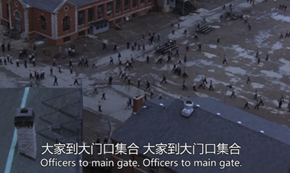
\includegraphics[scale=1.2]{./Chapter1/Figures/figure-film-subtitles.jpg}
    \caption{电影字幕}
    \label{fig:1-13}
\end{figure}
%-------------------------------------------

\parinterval (四)社交

\parinterval 社交是人们的重要社会活动。人们可以通过各种各样的社交软件做到即时通讯,进行协作或者分享自己的观点。然而受限于语言问题,人们的社交范围往往不会超出自己所掌握的语种范围,很难方便地进行跨语言社交。随着机器翻译技术的发展,越来越多的社交软件开始支持自动翻译,用户可以轻易地将各种语言的内容翻译成自己的母语,方便了人们的交流,让语言问题不再成为社交的障碍。

\parinterval (五)同声传译

\parinterval 在一些国际会议中,与会者来自许多不同的国家,为了保证会议的流畅,通常需要专业译员进行同声传译。同声传译需要在不打断演讲的同时,不间断地将讲话内容进行口译,对翻译人员的素质要求极高,成本高昂。现在,一些会议开始采用语音识别来将语音转换成文本,同时使用机器翻译技术进行翻译的方式,达到同步翻译的目的。这项技术已经得到了多个企业的关注,并在很多重要会议上进行尝试,取得了很好的反响。不过同声传译达到真正的使用还需一定时间的打磨,特别是会议场景下,准确进行语音识别和翻译仍然具有挑战性。

\parinterval (六)医药领域翻译

\parinterval 在医药领域中,从药品研发、临床试验到药品注册,都有着大量的翻译需求。比如,在新药注册阶段,限定申报时间的同时,更是对翻译质量有着极高的要求。由于医药领域专业词汇量庞大、单词冗长复杂、术语准确且文体专业性强,翻译难度明显高于其他领域,人工翻译的方式代价大且很难满足效率的要求。为此,机器翻译近几年在医药领域取得广泛应用。在针对医药领域进行优化后,机器翻译质量可以很好地满足翻译的要求。

\parinterval (七)中国传统语言文化的翻译

\parinterval 中国几千年的历史留下了极为宝贵的文化遗产,而其中,文言文作为古代书面语,具有言文分离、行文简练的特点,易于流传。言文分离的特点使得文言文和现在的标准汉语具有一定的区别。为了更好发扬中国传统文化,我们需要对文言文进行翻译。而文言文古奥难懂,人们需要具备一定的文言文知识背景才能准确翻译。机器翻译技术也可以帮助人们快速完成文言文的翻译。除此之外,机器翻译技术同样可以用于古诗生成和对联生成等任务。

\parinterval (八)全球化

\parinterval 在经济全球化的今天,很多企业都有国际化的需求,企业员工或多或少地会遇到一些跨语言阅读和交流的情况,比如阅读进口产品的说明书,跨国公司之间的邮件、说明文件等等。相比于成本较高的人工翻译,机器翻译往往是一种很好的选择。在一些质量要求不高的翻译场景中,机器翻译可以得到应用。

\parinterval (九)翻译机

\parinterval 出于商务、学术交流或者旅游的目的,人们在出国时会面临着跨语言交流的问题。近几年,随着出境人数的增加,不少企业推出了翻译机产品。通过结合机器翻译、语音识别和图像识别技术,翻译机实现了图像翻译和语音翻译的功能。用户可以很便捷地获取一些外语图像文字和语音信息,同时可以通过翻译机进行对话,降低跨语言交流门槛。

\parinterval (十)翻译结果后编辑

\parinterval 翻译结果后编辑是指在机器翻译的结果之上,通过少量的人工编辑来进一步完善机器译文。在传统的人工翻译过程中,翻译人员完全依靠人工的方式进行翻译,这虽然保证了翻译质量,但是时间成本高。相对应的,机器翻译具有速度快和成本低的优势。在一些领域,目前的机器翻译质量已经可以很大程度上减小翻译人员的工作量,翻译人员可以在机器翻译的辅助下,花费相对较小的代价来完成翻译。

%----------------------------------------------------------------------------------------
%    NEW SECTION
%----------------------------------------------------------------------------------------

\sectionnewpage
\section{开源项目与评测}

\parinterval 从实践的角度,机器翻译的发展主要可以归功于两方面的推动作用:开源系统和评测。开源系统通过代码共享的方式使得最新的研究成果可以快速传播,同时实验结果可以复现。而评测比赛,使得各个研究组织的成果可以进行科学的对比,共同推动机器翻译的发展与进步。此外,开源项目也促进了不同团队之间的协作,让研究人员在同一个平台上集中力量攻关。

%----------------------------------------------------------------------------------------
%    NEW SUB-SECTION
%----------------------------------------------------------------------------------------

\subsection{开源机器翻译系统}


下面列举一些优秀的开源机器翻译系统:

%----------------------------------------------------------------------------------------
%    NEW SUBSUB-SECTION
%----------------------------------------------------------------------------------------

\subsubsection{统计机器翻译开源系统}

\begin{itemize}
\vspace{0.5em}
\item NiuTrans.SMT。NiuTrans\cite{Tong2012NiuTrans}是由东北大学自然语言处理实验室自主研发的统计机器翻译系统,该系统可支持基于短语的模型、基于层次短语的模型以及基于句法的模型。由于使用C++ 语言开发,所以该系统运行时间快,所占存储空间少。系统中内嵌有$n$-gram语言模型,故无需使用其他的系统即可对完成语言建模。网址:\url{http://opensource.niutrans.com/smt/index.html}
\vspace{0.5em}
\item Moses。Moses\cite{Koehn2007Moses}是统计机器翻译时代最著名的系统之一,(主要)由爱丁堡大学的机器翻译团队开发。最新的Moses系统支持很多的功能,例如,它既支持基于短语的模型,也支持基于句法的模型。Moses 提供因子化翻译模型(Factored Translation Model),因此该模型可以很容易地对不同层次的信息进行建模。此外,它允许将混淆网络和字格作为输入,可缓解系统的1-best输出中的错误。Moses还提供了很多有用的脚本和工具,被机器翻译研究者广泛使用。网址:\url{http://www.statmt.org/moses/}
\vspace{0.5em}
\item Joshua。Joshua\cite{Li2010Joshua}是由约翰霍普金斯大学的语言和语音处理中心开发的层次短语翻译系统。由于Joshua是由Java语言开发,所以它在不同的平台上运行或开发时具有良好的可扩展性和可移植性。Joshua也是使用非常广泛的开源器翻译系统之一。网址:\url{https://cwiki.apache.org/confluence/display/JOSHUA/}
\vspace{0.5em}
\item SilkRoad。SilkRoad是由五个国内机构(中科院计算所、中科院软件所、中科院自动化所、厦门大学和哈尔滨工业大学)联合开发的基于短语的统计机器翻译系统。该系统是中国乃至亚洲地区第一个开源的统计机器翻译系统。SilkRoad支持多种解码器和规则提取模块,这样可以组合成不同的系统,提供多样的选择。网址:\url{http://www.nlp.org.cn/project/project.php?projid=14}
\vspace{0.5em}
\item SAMT。SAMT\cite{zollmann2007the}是由卡内基梅隆大学机器翻译团队开发的语法增强的统计机器翻译系统。SAMT在解码的时候使用目标树来生成翻译规则,而不严格遵守目标语言的语法。SAMT 的一个亮点是它提供了简单但高效的方式在机器翻译中使用句法信息。由于SAMT在hadoop中实现,它可受益于大数据集的分布式处理。网址:\url{http://www.cs.cmu.edu/zollmann/samt/}
\vspace{0.5em}
\item HiFST。HiFST\cite{iglesias2009hierarchical}是剑桥大学开发的统计机器翻译系统。该系统完全基于有限状态自动机实现,因此非常适合对搜索空间进行有效的表示。网址:\url{http://ucam-smt.github.io/}
\vspace{0.5em}
\item cdec。cdec\cite{dyer2010cdec}是一个强大的解码器,是由Chris Dyer 和他的合作者们一起开发。cdec的主要功能是它使用了翻译模型的一个统一的内部表示,并为结构预测问题的各种模型和算法提供了实现框架。所以,cdec也可以在被用来做一个对齐系统或者一个更通用的学习框架。此外,由于使用C++语言编写,cdec的运行速度较快。网址:\url{http://cdec-decoder.org/index.php?title=MainPage}
\vspace{0.5em}
\item Phrasal。Phrasal\cite{Cer2010Phrasal}是由斯坦福大学自然语言处理小组开发的系统。除了传统的基于短语的模型,Phrasal还支持基于非层次短语的模型,这种模型将基于短语的翻译延伸到非连续的短语翻译,增加了模型的泛化能力。网址:\url{http://nlp.stanford.edu/phrasal/}
\vspace{0.5em}
\item Jane。Jane\cite{vilar2012jane}是一个基于短语和基于层次短语的机器翻译系统,由亚琛工业大学的人类语言技术与模式识别小组开发。Jane提供了系统融合模块,因此可以非常方便的对多个系统进行融合。网址:\url{https://www-i6.informatik.rwth-aachen.de/jane/}
\vspace{0.5em}
\item GIZA++。GIZA++\cite{och2003systematic}是Franz Och研发的用于训练IBM模型1-5和HMM单词对齐模型的工具包。在早期,GIZA++是所有统计机器翻译系统中词对齐的标配工具。网址:\url{https://github.com/moses-smt/giza-pp}
\vspace{0.5em}
\item FastAlign。FastAlign\cite{dyer2013a}是一个快速,无监督的词对齐工具,由卡内基梅隆大学开发。网址:\url{https://github.com/clab/fast\_align}
\vspace{0.5em}
\end{itemize}

%----------------------------------------------------------------------------------------
%    NEW SUBSUB-SECTION
%----------------------------------------------------------------------------------------

\subsubsection{神经机器翻译开源系统}

\begin{itemize}
\vspace{0.5em}
\item GroundHog。GroundHog\cite{bahdanau2014neural}基于Theano\cite{al2016theano}框架,由蒙特利尔大学LISA 实验室使用Python语言编写的一个框架,旨在提供灵活而高效的方式来实现复杂的循环神经网络模型。它提供了包括LSTM在内的多种模型。Bahdanau等人在此框架上又编写了GroundHog神经机器翻译系统。该系统也作为了很多论文的基线系统。网址:\url{https://github.com/lisa-groundhog/GroundHog}
\vspace{0.5em}
\item Nematus。Nematus\cite{DBLP:journals/corr/SennrichFCBHHJL17}是英国爱丁堡大学开发的,基于Theano框架的神经机器翻译系统。该系统使用GRU作为隐层单元,支持多层网络。Nematus 编码端有正向和反向的编码方式,可以同时提取源语句子中的上下文信息。该系统的一个优点是,它可以支持输入端有多个特征的输入(例如词的词性等)。网址:\url{https://github.com/EdinburghNLP/nematus}
\vspace{0.5em}
\item ZophRNN。ZophRNN\cite{zoph2016simple}是由南加州大学的Barret Zoph 等人使用C++语言开发的系统。Zoph既可以训练序列表示模型(如语言模型),也可以训练序列到序列的模型(如神经机器翻译模型)。当训练神经机器翻译系统时,ZophRNN也支持多源输入。网址:\url{https://github.com/isi-nlp/Zoph\_RNN}
\vspace{0.5em}
\item Fairseq。Fairseq\cite{Ottfairseq}是由Facebook开发的,基于PyTorch框架的用以解决序列到序列问题的工具包,其中包括基于卷积神经网络、基于循环神经网络、基于Transformer的模型等。Fairseq是当今使用最广泛的神经机器翻译开源系统之一。网址:\url{https://github.com/facebookresearch/fairseq}
\vspace{0.5em}
\item Tensor2Tensor。Tensor2Tensor\cite{VaswaniTensor2Tensor}是由谷歌推出的,基于TensorFlow框架的开源系统。该系统基于Transformer模型,因此可以支持大多数序列到序列任务。得益于Transformer 的网络结构,系统的训练速度较快。现在,Tensor2Tensor也是机器翻译领域广泛使用的开源系统之一。网址:\url{https://github.com/tensorflow/tensor2tensor}
\vspace{0.5em}
\item OpenNMT。OpenNMT\cite{KleinOpenNMT}系统是由哈佛大学自然语言处理研究组开源的,基于Torch框架的神经机器翻译系统。OpenNMT系统的早期版本使用Lua 语言编写,现在也扩展到了TensorFlow和PyTorch,设计简单易用,易于扩展,同时保持效率和翻译精度。网址:\url{https://github.com/OpenNMT/OpenNMT}
\vspace{0.5em}
\item 斯坦福神经机器翻译开源代码库。斯坦福大学自然语言处理组(Stanford NLP)发布了一篇教程,介绍了该研究组在神经机器翻译上的研究信息,同时实现了多种翻译模型\cite{luong2016acl_hybrid}。 网址:\url{https://nlp.stanford.edu/projects/nmt/}
\vspace{0.5em}
\item THUMT。清华大学NLP团队实现的神经机器翻译系统,支持Transformer等模型\cite{ZhangTHUMT}。该系统主要基于TensorFlow和Theano实现,其中Theano版本包含了RNNsearch模型,训练方式包括MLE (Maximum Likelihood Estimate), MRT(Minimum Risk Training), SST(Semi-Supervised Training)。TensorFlow 版本实现了Seq2Seq, RNNsearch, Transformer三种基本模型。网址:\url{https://github.com/THUNLP-MT/THUMT}
\vspace{0.5em}
\item NiuTrans.NMT。由小牛翻译团队基于NiuTensor实现的神经机器翻译系统。支持循环神经网络、Transformer等结构,并支持语言建模、序列标注、机器翻译等任务。支持机器翻译GPU与CPU 训练及解码。其小巧易用,为开发人员提供快速二次开发基础。此外,NiuTrans.NMT已经得到了大规模应用,形成了支持187种语言翻译的小牛翻译系统。网址:\url{http://opensource.niutrans.com/niutensor/index.html}
\vspace{0.5em}
\item MARIAN。主要由微软翻译团队搭建\cite{JunczysMarian},其使用C++实现的用于GPU/CPU训练和解码的引擎,支持多GPU训练和批量解码,最小限度依赖第三方库,静态编译一次之后,复制其二进制文件就能在其他平台使用。网址:\url{https://marian-nmt.github.io/}
\vspace{0.5em}
\item Sockeye。由Awslabs开发的神经机器翻译框架\cite{hieber2017sockeye}。其中支持RNNsearch、Transformer、CNN等翻译模型,同时提供了从图片翻译到文字的模块以及WMT 德英新闻翻译、领域适应任务、多语言零资源翻译任务的教程。网址:\url{https://awslabs.github.io/sockeye/}
\vspace{0.5em}
\item CytonMT。由NICT开发的一种用C++实现的神经机器翻译开源工具包\cite{WangCytonMT}。主要支持Transformer模型,并支持一些常用的训练方法以及解码方法。网址:\url{https://github.com/arthurxlw/cytonMt}
\vspace{0.5em}
\item OpenSeq2Seq。由NVIDIA团队开发的\cite{DBLP:journals/corr/abs-1805-10387}基于TensorFlow的模块化架构,用于序列到序列的模型,允许从可用组件中组装新模型,支持混合精度训练,利用NVIDIA Volta Turing GPU中的Tensor核心,基于Horovod的快速分布式训练,支持多GPU,多节点多模式。网址:\url{https://nvidia.github.io/OpenSeq2Seq/html/index.html}
\vspace{0.5em}
\item NMTPyTorch。由勒芒大学语言实验室发布的基于序列到序列框架的神经网络翻译系统\cite{nmtpy2017},NMTPyTorch的核心部分依赖于Numpy,PyTorch和tqdm。其允许训练各种端到端神经体系结构,包括但不限于神经机器翻译、图像字幕和自动语音识别系统。网址:\url{https://github.com/lium-lst/nmtpytorch}
\vspace{0.5em}
\end{itemize}


%----------------------------------------------------------------------------------------
%    NEW SUB-SECTION
%----------------------------------------------------------------------------------------

\subsection{常用数据集及公开评测任务}

\parinterval 机器翻译相关评测主要有两种组织形式,一种是由政府及国家相关机构组织,权威性强。如由美国国家标准技术研究所组织的NIST评测、日本国家科学咨询系统中心主办的NACSIS Test Collections for IR(NTCIR)PatentMT、日本科学振兴机构(Japan Science and Technology Agency,简称JST)等组织联合举办的Workshop on Asian Translation(WAT)以及国内由中文信息学会主办的全国机器翻译大会(China Conference on Machine Translation,简称CCMT);另一种是由相关学术机构组织,具有领域针对性的特点,如倾向新闻领域的Conference on Machine Translation(WMT)以及面向口语的International Workshop on Spoken Language Translation(IWSLT)。下面将针对上述评测进行简要介绍。

\begin{itemize}
\vspace{0.5em}
\item CCMT(全国机器翻译大会),前身为CWMT(全国机器翻译研讨会)是国内机器翻译领域的旗舰会议,自2005年起已经组织多次机器翻译评测,对国内机器翻译相关技术的发展产生了深远影响。该评测主要针对汉语、英语以及国内的少数民族语言(蒙古语、藏语、维吾尔语等)进行评测,领域包括新闻、口语、政府文件等,不同语言方向对应的领域也有所不同。评价方式不同届略有不同,主要采用自动评价的方式,自CWMT\ 2013起则针对某些领域增设人工评价。自动评价的指标一般包括BLEU-SBP、BLEU-NIST、TER、METEOR、NIST、GTM、mWER、mPER 以及ICT 等,其中以BLEU-SBP 为主,汉语为目标语的翻译采用基于字符的评价方式,面向英语的翻译采用基于词的评价方式。每年该评测吸引国内外近数十家企业及科研机构参赛,业内认可度极高。关于CCMT的更多信息可参考中文信息学会机器翻译专业委员会相关页面:\url{http://sc.cipsc.org.cn/mt/index.php/CWMT.html}。
\vspace{0.5em}
\item WMT由Special Interest Group for Machine Translation(SIGMT)主办,会议自2006年起每年召开一次,是一个涉及机器翻译多种任务的综合性会议,包括多领域翻译评测任务、质量评价任务以及其他与机器翻译的相关任务(如文档对齐评测等)。现在WMT已经成为机器翻译领域的旗舰评测会议,很多研究工作都以WMT评测结果作为基准。WMT评测涉及的语言范围较广,包括英语、德语、芬兰语、捷克语、罗马尼亚语等十多种语言,翻译方向一般以英语为核心,探索英语与其他语言之间的翻译性能,领域包括新闻、信息技术、生物医学。最近,也增加了无指导机器翻译等热门问题。WMT在评价方面类似于CCMT,也采用人工评价与自动评价相结合的方式,自动评价的指标一般为BLEU、TER 等。此外,WMT公开了所有评测数据,因此也经常被机器翻译相关人员所使用。更多WMT的机器翻译评测相关信息可参考SIGMT官网:\url{http://www.sigmt.org/}。
\vspace{0.5em}
\item NIST机器翻译评测开始于2001年,是早期机器翻译公开评测中颇具代表性的任务,现在WMT和CCMT很多任务的设置也大量参考了当年NIST评测的内容。NIST评测由美国国家标准技术研究所主办,作为美国国防高级计划署(DARPA)中TIDES计划的重要组成部分。早期,NIST评测主要评价阿拉伯语和汉语等语言到英语的翻译效果,评价方法一般采用人工评价与自动评价相结合的方式。人工评价采用5分制评价。自动评价使用多种方式,包括BLEU,METEOR,TER以及HyTER。此外NIST从2016 年起开始对稀缺语言资源技术进行评估,其中机器翻译作为其重要组成部分共同参与评测,评测指标主要为BLEU。除对机器翻译系统进行评测之外,NIST在2008 和2010年对于机器翻译的自动评价方法(MetricsMaTr)也进行了评估,以鼓励更多研究人员对现有评价方法进行改进或提出更加贴合人工评价的方法。同时NIST评测所提供的数据集由于数据质量较高受到众多科研人员喜爱,如MT04,MT06等(汉英)平行语料经常被科研人员在实验中使用。不过,近几年NIST评测已经停止。更多NIST的机器翻译评测相关信息可参考官网:\url{https://www.nist.gov/programs-projects/machine-translation}。
\vspace{0.5em}
\item 从2004年开始举办的IWSLT也是颇具特色的机器翻译评测,它主要关注口语相关的机器翻译任务,测试数据包括TED talks的多语言字幕以及QED 教育讲座影片字幕等,语言涉及英语、法语、德语、捷克语、汉语、阿拉伯语等众多语言。此外在IWSLT 2016 中还加入了对于日常对话的翻译评测,尝试将微软Skype中一种语言的对话翻译成其他语言。评价方式采用自动评价的模式,评价标准和WMT类似,一般为BLEU 等指标。另外,IWSLT除了对文本到文本的翻译评测外,还有自动语音识别以及语音转另一种语言的文本的评测。更多IWSLT的机器翻译评测相关信息可参考IWSLT\ 2019官网:\url{https://workshop2019.iwslt.org/}。
\vspace{0.5em}
\item 日本举办的机器翻译评测WAT是亚洲范围内的重要评测之一,由日本科学振兴机构(JST)、情报通信研究机构(NICT)等多家机构共同组织,旨在为亚洲各国之间交流融合提供便宜之处。语言方向主要包括亚洲主流语言(汉语、韩语、印地语等)以及英语对日语的翻译,领域丰富多样,包括学术论文、专利、新闻、食谱等。评价方式包括自动评价(BLEU、RIBES以及AMFM 等)以及人工评价,其特点在于对于测试语料以段落为单位进行评价,考察其上下文关联的翻译效果。更多WAT的机器翻译评测相关信息可参考官网:\url{http://lotus.kuee.kyoto-u.ac.jp/WAT/}。
\vspace{0.5em}
\item NTCIR计划是由日本国家科学咨询系统中心策划主办的,旨在建立一个用在自然语言处理以及信息检索相关任务上的日文标准测试集。在NTCIR-9的和NTCIR-10中开设的Patent Machine Translation(PatentMT)任务主要针对专利领域进行翻译测试,其目的在于促进机器翻译在专利领域的发展和应用。在NTCIR-9中,评测方式采取人工评价与自动评价相结合,以人工评价为主导。人工评价主要根据准确度和流畅度进行评估,自动评价采用BLEU、NIST等方式进行。NTCIR-10评价方式在此基础上增加了专利审查评估、时间评估以及多语种评估,分别考察机器翻译系统在专利领域翻译的实用性、耗时情况以及不同语种的翻译效果等。更多NTCIR评测相关信息可参考官网:\url{http://research.nii.ac.jp/ntcir/index-en.html}。
\vspace{0.5em}
\end{itemize}

\parinterval 以上评测数据大多可以从评测网站上下载,此外部分数据也可以从LDC(Lingu-istic Data Consortium)上申请,网址为\url{https://www.ldc.upenn.edu/}。ELRA(Euro-pean Language Resources Association)上也有一些免费的语料库供研究使用,其官网为\url{http://www.elra.info/}。更多机器翻译的语料信息可参看附录\ref{appendix-A}。

\parinterval 从机器翻译发展的角度看,这些评测任务给相关研究提供了基准数据集,使得不同的系统都可以在同一个环境下进行比较和分析,进而建立了机器翻译研究所需的实验基础。此外,公开评测也使得研究者可以第一时间了解机器翻译研究的最新成果,比如,有多篇ACL会议最佳论文的灵感就来自当年参加机器翻译评测任务的系统。

%----------------------------------------------------------------------------------------
%    NEW SECTION
%----------------------------------------------------------------------------------------

\sectionnewpage
\section{推荐学习资源}

%----------------------------------------------------------------------------------------
%    NEW SUBSECTION
%----------------------------------------------------------------------------------------
\subsection{经典书籍}

\parinterval 首先,推荐一本书《Statistical Machine Translation》\cite{koehn2009statistical},其作者是机器翻译领域著名学者Philipp Koehn教授。该书是机器翻译领域内的经典之作,介绍了统计机器翻译技术的进展。该书从语言学和概率学两个方面介绍了统计机器翻译的构成要素,然后介绍了统计机器翻译的主要模型:基于词、基于短语和基于树的模型,以及机器翻译评价、语言建模、判别式训练等方法。此外,作者在该书的最新版本中增加了神经机器翻译的章节,方便研究人员全面了解机器翻译的最新发展趋势\cite{DBLP:journals/corr/abs-1709-07809}。

\parinterval 《Foundations of Statistical Natural Language Processing》\cite{manning1999foundations}中文译名《统计自然语言处理基础》,作者是自然语言处理领域的权威Chris Manning教授和Hinrich Sch$\ddot{\textrm{u}}$tze教授。该书对统计自然语言处理方法进行了全面介绍。书中讲解了统计自然语言处理所需的语言学和概率论基础知识,介绍了机器翻译评价、语言建模、判别式训练以及整合语言学信息等基础方法。其中也包含了构建自然语言处理工具所需的基本理论和算法,提供了对数学和语言学基础内容广泛而严格的覆盖,以及统计方法的详细讨论。

\parinterval 《统计自然语言处理》\cite{宗成庆2013统计自然语言处理}由中国科学院自动化所宗成庆教授所著。该书中系统介绍了统计自然语言处理的基本概念、理论方法和最新研究进展,既有对基础知识和理论模型的介绍,也有对相关问题的研究背景、实现方法和技术现状的详细阐述。可供从事自然语言处理、机器翻译等研究的相关人员参考。

\parinterval  Ian Goodfellow、Yoshua Bengio、Aaron Courville三位机器学习领域的学者所写的《Deep Learning》\cite{Goodfellow-et-al-2016}也是值得一读的参考书。其讲解了有关深度学习常用的方法,其中很多都会在深度学习模型设计和使用中用到。同时在该书的应用一章中也简单讲解了神经机器翻译的任务定义和发展过程。

\parinterval 《Neural Network Methods for Natural Language Processing》\cite{goldberg2017neural}是Yoav Goldberg编写的面向自然语言处理的深度学习参考书。相比《Deep Learning》,该书聚焦在自然语言处理中的深度学习方法,内容更加易读,非常适合刚入门自然语言处理及深度学习应用的人员参考。

\parinterval 《机器学习》\cite{周志华2016机器学习}由南京大学周志华教授所著,作为机器学习领域入门教材,该书尽可能地涵盖了机器学习基础知识的各个方面,试图尽可能少地使用数学知识介绍机器学习方法与思想。

\parinterval 《统计学习方法》\cite{李航2012统计学习方法}由李航博士所著,该书对机器学习的有监督和无监督等方法进行了全面而系统的介绍。可以作为梳理机器学习的知识体系,同时了解相关基础概念的参考读物。

\parinterval 《神经网络与深度学习》\cite{邱锡鹏2020神经网络与深度学习}由复旦大学邱锡鹏教授所著,全面地介绍了神经网络和深度学习的基本概念和常用技术,同时涉及了许多深度学习的前沿方法。该书适合初学者阅读,同时又不失为一本面向专业人士的参考书。

%----------------------------------------------------------------------------------------
%    NEW SUBSECTION
%----------------------------------------------------------------------------------------
\subsection{网络资源}

\parinterval  TensorFlow官网提供了一个有关神经机器翻译的教程,介绍了从数据处理开始如何利用TensorFlow工具从零搭建一个神经机器翻译系统以及如何解码,其地址为\url{https://www.tensorflow.org/tutorials/text/nmt\_with\_attention}。此外谷歌和Facebook也分别提供了基于序列到序列机器翻译模型的高级教程。谷歌的版本是基于TensorFlow实现,网址为:\url{https://github.com/tensorflow/nmt}。Facebook的教程主要是基于PyTorch实现,网址为:\url{https://pytorch.org/tutorials/intermediate/seq2seq\_translation\_tutorial.html}。网站上也包含一些综述论文,其中详细的介绍了神经机器翻译的发展历程,问题定义以及目前遇到的问题。

\parinterval  \url{http://www.statmt.org}是一个介绍机器翻译研究的网站,该网站包含了对统计机器翻译研究的一些介绍资料,一些自然语言处理的会议,常用工具以及语料库。\url{http://www.mt-archive.info}与\url{https://www.aclweb.org/anthology}网站上有许多介绍机器翻译和自然语言处理的论文,通过这些网站还可以了解到自然语言处理领域的一些重要期刊和会议。

%----------------------------------------------------------------------------------------
%    NEW SUBSECTION
%----------------------------------------------------------------------------------------
\subsection{专业组织和会议}

许多自然语言处理的相关学术组织会定期举办学术会议。与机器翻译相关的会议有:

\begin{itemize}
\vspace{0.5em}
\item ACL,全称Annual Conference of the Association for Computational Linguistics,是自然语言处理领域最高级别的会议。每年举办一次,主题涵盖计算语言学的所有方向。
\vspace{0.5em}
\item NAACL,全称Annual Conference of the North American Chapter of the Association for Computational Linguistics,为ACL北美分会,在自然语言处理领域也属于顶级会议,每年会选择一个北美城市召开会议。
\vspace{0.5em}
\item EMNLP,全称Conference on Empirical Methods in Natural Language Processing ,自然语言处理另一个顶级会议之一,由ACL当中对语言数据和经验方法有特殊兴趣的团体主办,始于1996年。会议比较偏重于方法和经验性结果。
\vspace{0.5em}
\item COLING,全称International Conference on Computational Linguistics,自然语言处理老牌顶级会议之一。该会议始于1965年,是由ICCL国际计算语言学委员会主办。会议简称为COLING,是谐音瑞典著名作家 Albert Engstr$\ddot{\textrm{o}}$m小说中的虚构人物Kolingen。COLING每两年举办一次。
\vspace{0.5em}
\item EACL,全称Conference of the European Chapter of the Association for Computational Linguistics,为ACL欧洲分会,虽然在欧洲召开,会议也吸引了全世界的大量学者投稿并参会。
\vspace{0.5em}
\item AACL,全称Conference of the Asia-Pacific Chapter of the Association for Computational Linguistics,为ACL亚太地区分会。2020年会议首次召开,是亚洲地区自然语言处理领域最具影响力的会议之一。
\vspace{0.5em}
\item WMT,全称Conference on Machine Translation。机器翻译领域一年一度研讨会,是国际公认的顶级机器翻译赛事之一。
\vspace{0.5em}
\item AMTA,全称Conference of the Association for Machine Translation in the Americas。AMTA会议汇聚了学术界、产业界和政府的研究人员、开发人员和用户,让工业界和学术界进行交流。
\vspace{0.5em}
\item CCL,全称China National Conference on Computational Linguistics,中文为中国计算语言学大会。中国计算语言学大会创办于1991年,由中国中文信息学会计算语言学专业委员会负责组织。经过20余年的发展,中国计算语言学大会已成为国内自然语言处理领域权威性最高、规模和影响最大的学术会议。作为中国中文信息学会(国内一级学会)的旗舰会议,CCL聚焦于中国境内各类语言的智能计算和信息处理,为研讨和传播计算语言学最新学术和技术成果提供了最广泛的高层次交流平台。
\vspace{0.5em}
\item NLPCC,全称CCF International Conference on Natural Language Processing and Chinese Computing。NLPCC 是由中国计算机学会(CCF)主办的 CCF 中文信息技术专业委员会年度学术会议,专注于自然语言处理及中文处理领域的研究和应用创新。会议自 2012 年开始举办,主要活动有主题演讲、论文报告、技术测评等多种形式。
\vspace{0.5em}
\item CCMT,全称China Conference on Machine Translation,中国机器翻译研讨会,由中国中文信息学会主办,旨在为国内外机器翻译界同行提供一个平台,促进中国机器翻译事业。CCMT不仅是国内机器翻译领域最具影响力、最权威的学术和评测活动,而且也代表着汉语与民族语言翻译技术的最高水准,对民族语言技术发展具有重要意义。
\vspace{0.5em}
\end{itemize}

除了会议之外,《中文信息学报》、《Computational Linguistics》、《Machine Translation》、《Transactions of the Association for Computational Linguistics》、《IEEE/ACM Transactions on Audio, Speech, and Language Processing》、《ACM Transactions on Asian and Low Resource Language Information Processing》、《Natural Language Engineering》等期刊也发表了许多与机器翻译相关的重要论文。











% !Mode:: "TeX:UTF-8"
% !TEX encoding = UTF-8 Unicode

%----------------------------------------------------------------------------------------
% 机器翻译:统计建模与深度学习方法
% Machine Translation: Statistical Modeling and Deep Learning Methods
%
% Copyright 2020
% 肖桐(xiaotong@mail.neu.edu.cn) 朱靖波 (zhujingbo@mail.neu.edu.cn)
%----------------------------------------------------------------------------------------

%----------------------------------------------------------------------------------------
%    CONFIGURATIONS
%----------------------------------------------------------------------------------------

\renewcommand\figurename{图}%将figure改为图
\renewcommand\tablename{表}%将figure改为图
%\renewcommand\arraystretch{1.5}%将表格高度调整为1.5倍
\chapterimage{fig-NEU-3.jpg} % Chapter heading image

%----------------------------------------------------------------------------------------
%	CHAPTER 2
%----------------------------------------------------------------------------------------

\chapter{词法、语法及统计建模基础}

\parinterval 机器翻译并非是一个孤立的系统,它依赖于很多模块,并且需要很多学科知识的融合。现在的机器翻译系统大多使用统计模型对翻译问题进行建模,同时也会用到一些自然语言处理工具来对不同语言的文字进行分析。因此,在正式开始机器翻译内容的介绍之前,本章将会对相关的基础知识进行概述,包括:概率论与统计建模基础、语言分析、语言建模等。

\parinterval 概率论与统计建模是机器翻译方法的基础。这里会对机器翻译所涉及的基本数学概念进行简要描述,确保后续使用到的数学工具是完备的。本章会重点关注如何利用统计建模的方式对自然语言处理问题进行描述,这种手段在统计机器翻译和神经机器翻译中会被使用。

\parinterval 语言分析部分将以汉语为例介绍词法和句法分析的基本概念。它们都是自然语言处理中的经典问题,而且在机器翻译中也会经常被使用。同样,本章会介绍这两个任务的定义和求解问题的思路。

\parinterval 语言建模是机器翻译中最常用的一种技术,它主要用于句子的生成和流畅度评价。本章会以传统统计语言模型为例,对语言建模的相关概念进行介绍。但是,这里并不深入探讨语言模型技术,在后面的章节中还会单独对神经网络语言模型等前沿技术进行讨论。

%----------------------------------------------------------------------------------------
%    NEW SECTION
%----------------------------------------------------------------------------------------

\section{问题概述 }

\parinterval 很多时候机器翻译系统被看作是孤立的``黑盒''系统(图 \ref {fig:2-1} (a))。将一段文本作为输入送入机器翻译系统之后,系统输出翻译好的译文。但是真实的机器翻译系统非常复杂,因为系统看到的输入和输出实际上只是一些符号串,这些符号并没有任何意义,因此需要进一步对这些符号串进行处理才能更好的使用它们。比如,需要定义翻译中最基本的单元是什么?符号串是否具有结构信息?如何用数学工具刻画这些基本单元和结构?

%----------------------------------------------
\begin{figure}[htp]
    \centering
 	\subfigure[机器翻译系统被看作一个黑盒] {\input{./Chapter2/Figures/figure-mt-system-as-a-black-box}  }
 	\subfigure[机器翻译系统 = 前/后处理 + 翻译引擎] {\input{./Chapter2/Figures/figure-mt=language-analysis+translation-engine}}
	\caption{机器翻译系统的结构}
    \label{fig:2-1}
\end{figure}
%-------------------------------------------

%----------------------------------------------
\begin{figure}[htp]
\centering

%%% outline
%-------------------------------------------------------------------------

\vspace{0.3em}
\begin{tikzpicture}


\begin{scope}[scale=1.0,level distance=30pt,sibling distance=15pt,grow'=up]
{
\Tree[.\node(sn0){IP};
          [.\node(sn1){NP};
               [.\node(sn2){NN}; \node(sw1){猫}; ]
          ]
          [.\node(sn3){VP};
               [.\node(sn4){VV}; \node(sw2){喜欢}; ]
               [.\node(sn5){VP}; \edge[roof]; \node(sw3){吃 \ 鱼}; ]
          ]
     ]
}
\end{scope}

\end{tikzpicture}

%---------------------------------------------------------------------

\caption{中文句子``猫喜欢吃鱼''的分析结果(分词和句法分析)}
\label{fig:2-2}
\end{figure}
%-------------------------------------------

\parinterval 图\ref{fig:2-1} (b)展示了一个机器翻译系统的输入和输出形式。可以看到,输入的中文词串``猫喜欢吃鱼''被加工成一个新的结构(图\ref {fig:2-2})。直觉上,这个结构有些奇怪,因为上面多了很多新的符号,而且还有一些线将不同符号进行连接。实际上这就是语言分析中对句子常用的结构表示 —— 短语结构树。从原始的词串转化为图\ref {fig:2-2} 的样子,有两个步骤:

\begin{itemize}
\vspace{0.5em}
\item {\small\bfnew{分词}}\index{分词}(Segmentation)\index{Segmentation}:这个过程会把词串进行切分,切割成最小的单元。因为只有知道了什么是待处理字符串的最小单元,机器翻译系统才能对其进行表示、分析和生成。
\vspace{0.5em}
\item {\small\bfnew{句法分析}}\index{句法分析}(Parsing)\index{Parsing}:这个过程会对分词的结果进行进一步分析,得到句子的句法结构。这种结构是对句子的进一步抽象,比如,NP+VP就可以表示由名词短语(NP)和动词短语(VP)构成的主谓结构。利用这些信息,机器翻译可以更加准确地对语言的结构进行分析和生成。
\vspace{0.5em}
\end{itemize}

\parinterval 类似地,机器翻译输出的结果也可以包含同样的信息。甚至系统输出英文译文之后,还有一个额外的步骤来把部分英文单词的大小写恢复出来,比如,上例中句首单词Cats的首字母要大写。

\parinterval 一般来说,在送入机器翻译系统前需要对文字序列进行处理和加工,这个过程被称为{\small\sffamily\bfseries{预处理}}\index{预处理}(Pre-processing)\index{Pre-processing}。同理,在机器翻译模型输出译文后进行的处理被称作{\small\sffamily\bfseries{后处理}}\index{后处理}(Post-processing)\index{Post-processing}。这两个过程对机器翻译性能影响很大,比如,在神经机器翻译里,不同的分词策略可能会造成翻译性能的天差地别。

\parinterval 值得注意的是,有些观点认为,不论是分词还是句法分析,对于机器翻译来说并不要求符合人的认知和语言学约束。换句话说,机器翻译所使用的``单词''和``结构''本身并不是为了符合人类的解释,它们更直接目的是为了进行翻译。从系统开发的角度,有时候即使是一些与人类的语言习惯有差别的处理,仍然会带来性能的提升,比如在神经机器翻译中,在传统分词的基础上进一步使用双字节编码(Byte Pair Encoding,BPE)子词切分会使得机器翻译性能大幅提高。当然,自然语言处理中语言学信息的使用一直是学界关注的焦点。甚至关于语言学结构对机器翻译是否有作用这个问题也有争论。但是不能否认的是,无论是语言学的知识,还是计算机自己学习到的知识,对机器翻译都是有价值的。在后续章节会看到,这两种类型的知识对机器翻译帮助很大 \footnote[1]{笔者并不认同语言学结构对机器翻译的帮助有限,相反机器翻译需要更多的人类先验知识的指导。当然,这个问题不是这里讨论的重点。} 。

\parinterval 剩下的问题是如何进行句子的切分和结构的分析。思路有很多,一种常用的方法是对问题进行概率化,用统计模型来描述问题并求解之。比如,一个句子切分的好坏,并不是非零即一的判断,而是要估计出这种切分的可能性大小,最终选择可能性最大的结果进行输出。这也是一种典型的用统计建模的方式来描述自然语言处理问题的方法。

\parinterval 本章将会对上述问题及求解问题的方法进行介绍。首先,会用一个例子给出统计建模的基本思路,之后会应用这种方法进行中文分词、语言建模和句法分析。
\vspace{-1em}

%----------------------------------------------------------------------------------------
%    NEW SECTION
%----------------------------------------------------------------------------------------

\sectionnewpage
\section{概率论基础}
\parinterval 为了便于后续内容的介绍,首先对本书中使用的概率和统计学概念进行说明。

%----------------------------------------------------------------------------------------
%    NEW SUB-SECTION
%----------------------------------------------------------------------------------------

\subsection{随机变量和概率}
\parinterval 在自然界中,很多{\small\bfnew{事件}}\index{事件}(Event)\index{Event}是否会发生是不确定的。例如,明天会下雨、掷一枚硬币是正面朝上、扔一个骰子的点数是5$\cdots\cdots$这类事件可能会发生也可能不会发生。通过大量的重复试验,能发现其具有某种规律性的事件叫做{\small\sffamily\bfseries{随机事件}}\index{随机事件}。

\parinterval {\small\sffamily\bfseries{随机变量}}\index{随机变量}(Random Variable)\index{Random Variable}是对随机事件发生可能状态的描述,是随机事件的数量表征。设$\Omega = \{ \omega \}$为一个随机试验的样本空间,$X=X(\omega)$就是定义在样本空间$\Omega$上的单值实数函数,即$X=X(\omega)$为随机变量,记为$X$。随机变量是一种能随机选取数值的变量,常用大写的英文字母或希腊字母表示,其取值通常用小写字母来表示。例如,用$A$ 表示一个随机变量,用$a$表示变量$A$的一个取值。根据随机变量可以选取的值的某些性质,可以将其划分为离散变量和连续变量。

\parinterval 离散变量是指在其取值区间内可以被一一列举,总数有限并且可计算的数值变量。例如,用随机变量$X$代表某次投骰子出现的点数,点数只可能取1$\sim$6这6个整数,$X$就是一个离散变量。

\parinterval 连续变量是在其取值区间内连续取值,无法被一一列举,具有无限个取值的变量。例如,图书馆的开馆时间是8:30-22:00,用$X$代表某人进入图书馆的时间,时间的取值范围是[8:30,22:00]这个时间区间,$X$就是一个连续变量。

\parinterval {\small\bfnew{概率}}\index{概率}(Probability)\index{Probability}是度量随机事件呈现其每个可能状态的可能性的数值,本质上它是一个测度函数\cite{mao-prob-book-2011}\cite{kolmogorov2018foundations}。概率的大小表征了随机事件在一次试验中发生的可能性大小。用$\textrm{P}(\cdot )$表示一个随机事件的可能性,即事件发生的概率。比如$\textrm{P}(\textrm{太阳从东方升起})$表示``太阳从东方升起的可能性'',同理,$\textrm{P}(A=B)$ 表示的就是``$A=B$'' 这件事的可能性。

\parinterval 在实际问题中,往往需要得到随机变量的概率值。但是,真实的概率值可能是无法准确知道的,这时就需要对概率进行{\small\sffamily\bfseries{估计}}\index{估计},得到的结果是概率的{\small\sffamily\bfseries{估计值}}\index{估计值}(Estimate)\index{Estimate}。在概率论中,一个很简单的方法是利用相对频度作为概率的估计值。如果$\{x_1,x_2,\dots,x_n \}$是一个试验的样本空间,在相同情况下重复试验$N$次,观察到样本$x_i (1\leq{i}\leq{n})$的次数为$n (x_i )$,那么$x_i$在这$N$次试验中的相对频率是$\frac{n(x_i )}{N}$。当$N$越来越大时,相对概率也就越来越接近真实概率$\textrm{P}(x_i)$,即$\lim_{N \to \infty}\frac{n(x_i )}{N}=\textrm{P}(x_i)$。 实际上,很多概率模型都等同于相对频度估计,比如,对于一个服从多项式分布的变量的极大似然估计就可以用相对频度估计实现。

%--------------------------------------------------------------------
\begin{table}[htp]
\centering
\caption{离散变量$A$的概率分布}
\begin{tabular}{c|c c c c c c}
\rule{0pt}{15pt}     $A$ & $a_1=1$ & $a_2=2$ & $a_3=3$ & $a_4=4$ & $a_5=5$ & $a_6=6$\\
               \hline
\rule{0pt}{15pt}     $\textrm{P}_i$ & $\textrm{P}_1=\frac{4}{25}$  &  $\textrm{P}_2=\frac{3}{25}$ &  $\textrm{P}_3=\frac{4}{25}$ & $\textrm{P}_4=\frac{6}{25}$ & $\textrm{P}_5=\frac{3}{25}$ & $\textrm{P}_6=\frac{1}{25}$  \\
             \end{tabular}
             \label{tab:2-1}
\end{table}
%--------------------------------------------------------------------

\parinterval 概率函数是用函数形式给出离散变量每个取值发生的概率,其实就是将变量的概率分布转化为数学表达形式。如果把$A$看做一个离散变量,$a$看做变量$A$的一个取值,那么$\textrm{P}(A)$被称作变量$A$的概率函数,$\textrm{P}(A=a)$被称作$A = a$的概率值,简记为$\textrm{P}(a)$。例如,在相同条件下掷一个骰子50次,用$A$表示投骰子出现的点数这个离散变量,$a_i$表示点数的取值,$\textrm{P}_i$表示$A=a_i$的概率值。表\ref{tab:2-1}为$A$的概率分布,给出了$A$的所有取值及其概率。

\parinterval 除此之外,概率函数$\textrm{P}(\cdot)$还具有非负性、归一性等特点。非负性是指,所有的概率函数$\textrm{P}(\cdot)$都必须是大于等于0的数值,概率函数中不可能出现负数,即$\forall{x},\textrm{P}{(x)}\geq{0}$。归一性,又称规范性,简单的说就是所有可能发生的事件的概率总和为1,即$\sum_{x}\textrm{P}{(x)}={1}$。

%----------------------------------------------
\begin{figure}[htp]
\centering
 \input{./Chapter2/Figures/figure-probability-density-function&distribution-function}
\caption{一个概率密度函数(左)与其对应的分布函数(右)}
\label{fig:2-3}
\end{figure}
%-------------------------------------------

\parinterval 对于离散变量$A$,$\textrm{P}(A=a)$是个确定的值,可以表示事件$A=a$的可能性大小;而对于连续变量,求在某个定点处的概率是无意义的,只能求其落在某个取值区间内的概率。因此,用{\small\sffamily\bfseries{概率分布函数}}\index{概率分布函数}$F(x)$和{\small\sffamily\bfseries{概率密度函数}}\index{概率密度函数}$f(x)$来统一描述随机变量取值的分布情况(如图\ref{fig:2-3})。概率分布函数$F(x)$表示取值小于等于某个值的概率,是概率的累加(或积分)形式。假设$A$是一个随机变量,$a$是任意实数,将函数$F(a)=\textrm{P}\{A\leq a\}$,$-\infty<a<\infty $定义为$A$的分布函数。通过分布函数,可以清晰地表示任何随机变量的概率。

\parinterval 概率密度函数反映了变量在某个区间内的概率变化快慢,概率密度函数的值是概率的变化率,该连续变量的概率也就是对概率密度函数求积分得到的结果。设$f(x) \geq 0$是连续变量$X$的概率密度函数,$X$的分布函数就可以用如下公式定义:
\begin{eqnarray}
F(x)=\int_{-\infty}^x f(x)dx
\label{eq:2-1}
\end{eqnarray}

%----------------------------------------------------------------------------------------
%    NEW SUB-SECTION
%----------------------------------------------------------------------------------------

\subsection{联合概率、条件概率和边缘概率}
\parinterval {\small\sffamily\bfseries{联合概率}}\index{联合概率}(Joint Probability)\index{Joint Probability}是指多个事件共同发生,每个随机变量满足各自条件的概率,表示为$\textrm{P}(AB)$或$\textrm{P}(A\cap{B})$。{\small\sffamily\bfseries{条件概率}}\index{条件概率}(Conditional Probability)\index{Conditional Probability}是指$A$、$B$为任意的两个事件,在事件$A$已出现的前提下,事件$B$出现的概率,使用$\textrm{P}(B \mid A)$表示。

\parinterval 贝叶斯法则(见\ref{sec:2.2.3}小节)是条件概率计算时的重要依据,条件概率可以表示为
\begin{eqnarray}
\textrm{P}{(B|A)} & = & \frac{\textrm{P}(A\cap{B})}{\textrm{P}(A)}  \nonumber \\
                           & = & \frac{\textrm{P}(A)\textrm{P}(B|A)}{\textrm{P}(A)}  \nonumber \\
                           & = & \frac{\textrm{P}(B)\textrm{P}(A|B)}{\textrm{P}(A)}
\label{eq:2-2}
\end{eqnarray}

\parinterval {\small\sffamily\bfseries{边缘概率}}\index{边缘概率}(marginal probability)\index{marginal probability}是和联合概率对应的,它指的是$\textrm{P}(X=a)$或$\textrm{P}(Y=b)$,即仅与单个随机变量有关的概率。对于离散随机变量$X$和$Y$,如果知道$\textrm{P}(X,Y)$,则边缘概率$\textrm{P}(X)$可以通过求和的方式得到。对于$\forall x \in X $,有
\begin{eqnarray}
\textrm{P}(X=x)=\sum_{y}  \textrm{P}(X=x,Y=y)
\label{eq:2-3}
\end{eqnarray}

\parinterval 对于连续变量,边缘概率$\textrm{P}(X)$需要通过积分得到,如下式所示
\begin{eqnarray}
\textrm{P}(X=x)=\int \textrm{P}(x,y)dy
\label{eq:2-4}
\end{eqnarray}

\parinterval 为了更好地区分条件概率、边缘概率和联合概率,这里用一个图形面积的计算来举例说明。如图\ref{fig:2-4}所示,矩形$A$代表事件$X$发生所对应的所有可能状态,矩形$B$代表事件$Y$发生所对应的所有可能状态,矩形$C$代表$A$和$B$的交集,则

\begin{itemize}
\vspace{0.5em}
\item 边缘概率:矩形$A$或者矩形$B$的面积;
\vspace{0.5em}
\item 联合概率:矩形$C$的面积;
\vspace{0.5em}
\item 条件概率:联合概率/对应的边缘概率,如:$\textrm{P}(A \mid B)$=矩形$C$的面积/矩形B的面积。
\vspace{0.5em}
\end{itemize}

%----------------------------------------------
\begin{figure}[htp]
\centering

%%% outline
%-------------------------------------------------------------------------
\begin{tikzpicture}



\begin{scope}[scale=1.0]
{

\node [anchor=north west,minimum width=7em, minimum height=2.5em,fill=blue!30](num1)  at (0,0) {$A$\quad \quad \quad \quad  };
\node [anchor=west,minimum width=7em, minimum height=5em,fill=ugreen!30](num2)  at ([xshift=-3em]num1.east) {\quad \quad $B$};
\node [anchor=west,minimum width=3em, minimum height=2.5em,fill=yellow!30](part1)  at (num2.west) {$C$};

\draw [-,thick] (num1.north west) -- (num1.north east) -- (num1.south east) -- (num1.south west) -- (num1.north west);
\draw [-,very thick,dotted] (num2.north west) -- (num2.north east) -- (num2.south east) -- (num2.south west) -- (num2.north west);

}
\end{scope}
\end{tikzpicture}
%---------------------------------------------------------------------


\caption{$A$、$B$、$C$事件所对应概率的图形化表示}
\label{fig:2-4}
\end{figure}
%-------------------------------------------

%----------------------------------------------------------------------------------------
%    NEW SUB-SECTION
%----------------------------------------------------------------------------------------

\subsection{链式法则}

\parinterval 条件概率公式$\textrm{P}(A \mid B)=\textrm{P}(AB)/\textrm{P}(B)$反映了事件$B$发生的条件下事件$A$发生的概率。如果将其推广到三个事件$A$、$B$、$C$,为了计算$\textrm{P}(A,B,C)$,我们可以运用两次$\textrm{P}(A \mid B)=\textrm{P}(AB)/\textrm{P}(B)$,计算过程如下:
\begin{eqnarray}
\textrm{P}(A,B,C) & = & \textrm{P}(A \mid B ,C)\textrm{P}(B,C) \nonumber \\
                           & = & \textrm{P}(A \mid B,C)\textrm{P}(B \mid C)\textrm{P}(C)
\label{eq:2-5}
\end{eqnarray}

\parinterval 推广到$n$个事件,可以得到了链式法则的公式
\begin{eqnarray}
\textrm{P}(x_1,x_2,...,x_n)=\textrm{P}(x_1) \prod_{i=2}^n \textrm{P}(x_i \mid x_1,x_2,...,x_{i-1})
\label{eq:2-6}
\end{eqnarray}

\parinterval 下面的例子有助于更好的理解链式法则,如图\ref{fig:2-5}所示,$A$、$B$、$C$、$D$、\\ $E$分别代表五个事件,其中,$A$只和$B$有关,$C$只和$B$、$D$有关,$E$只和$C$有关,$B$和$D$不依赖其他任何事件。则$\textrm{P}(A,B,C,D,E)$的表达式如下式:

%----------------------------------------------
\begin{figure}[htp]
\centering


%%% outline
%-------------------------------------------------------------------------
\begin{tikzpicture}


\node [anchor=north west](num1)  at (0,0) {\large{A}};
\node [anchor=north west](num2)  at ([xshift=5.8em,yshift=1.44em]num1.south west) {\large{B}};
\node [anchor=north west](num3)  at ([xshift=5.8em,yshift=1.44em]num2.south west) {\large{C}};
\node [anchor=north west](num4)  at ([xshift=5.8em,yshift=1.44em]num3.south west) {\large{D}};
\node [anchor=north west](num5)  at ([xshift=0.04em,yshift=-2.5em]num3.south west) {\large{E}};


\draw [<-,very thick,black] (num1.east)--(num2.west);
\draw [->,very thick,black] (num2.east)--(num3.west);
\draw [<-,very thick,black] (num3.east)--(num4.west);
\draw [->,very thick,black] (num3.south)--(num5.north);



\end{tikzpicture}

\setlength{\belowcaptionskip}{-1cm}
\caption{事件$A$、$B$、$C$、$D$、$E$之间的关系图}
\label{fig:2-5}
\end{figure}
%-------------------------------------------

\begin{eqnarray}
&   & \textrm{P}(A,B,C,D,E) \nonumber \\
&=&\textrm{P}(E \mid A,B,C,D) \cdot \textrm{P}(A,B,C,D) \nonumber \\
&=&\textrm{P}(E \mid A,B,C,D) \cdot \textrm{P}(D \mid A,B,C) \cdot \textrm{P}(A,B,C) \nonumber \\
&=&\textrm{P}(E \mid A,B,C,D) \cdot \textrm{P}(D \mid A,B,C) \cdot \textrm{P}(C \mid A,B) \cdot \textrm{P}(A,B) \nonumber \\
&=&\textrm{P}(E \mid A,B,C,D) \cdot \textrm{P}(D \mid A,B,C) \cdot \textrm{P}(C \mid A,B) \cdot \textrm{P}(B \mid A) \cdot \textrm{P}(A)
\label{eq:2-7}
\end{eqnarray}

\parinterval 根据图\ref {fig:2-5} 易知$E$只和$C$有关,所以$\textrm{P}(E \mid A,B,C,D)=\textrm{P}(E \mid C)$;$D$不依赖于其他事件,所以$\textrm{P}(D \mid A,B,C)=\textrm{P}(D)$;$C$只和$B$、$D$有关,所以$\textrm{P}(C \mid A,B)=\textrm{P}(C \mid B)$;$B$不依赖于其他事件,所以$\textrm{P}(B \mid  A)=\textrm{P}(B)$。最终化简可得:
\begin{eqnarray}
\textrm{P}(A,B,C,D,E)=\textrm{P}(E \mid C) \cdot \textrm{P}(D) \cdot \textrm{P}(C \mid B) \cdot \textrm{P}(B)\cdot \textrm{P}(A \mid B)
\label{eq:2-8}
\end{eqnarray}

%----------------------------------------------------------------------------------------
%    NEW SUB-SECTION
%----------------------------------------------------------------------------------------

\subsection{贝叶斯法则}\label{sec:2.2.3}

\parinterval 首先介绍一下全概率公式:{\small\bfnew{全概率公式}}\index{全概率公式}(Law of Total Probability)\index{Law of Total Probability}是概率论中重要的公式,它可以将一个复杂事件发生的概率分解成不同情况的小事件发生概率的和。这里先介绍一个概念——划分。集合$S$的一个划分事件为$\{B_1,...,B_n\}$是指它们满足$\bigcup_{i=1}^n B_i=S \textrm{且}B_iB_j=\varnothing , i,j=1,...,n,i\neq j$。此时事件$A$的全概率公式可以被描述为:

\begin{eqnarray}
\textrm{P}(A)=\sum_{k=1}^n \textrm{P}(A \mid B_k)\textrm{P}(B_k)
\label{eq:2-9}
\end{eqnarray}

\parinterval 举个例子,小张从家到公司有三条路分别为$a$,$b$,$c$,选择每条路的概率分别为0.5,0.3,0.2。令:

\begin{itemize}
\vspace{0.5em}
\item $S_a$:小张选择$a$路去上班
\vspace{0.5em}
\item $S_b$:小张选择$b$路去上班
\vspace{0.5em}
\item $S_c$:小张选择$c$路去上班
\vspace{0.5em}
\item $S$:小张去上班
\vspace{0.5em}
\end{itemize}

\parinterval 显然,$S_a$,$S_b$,$S_c$是$S$的划分。如果三条路不拥堵的概率分别为$\textrm{P}({S_{a}^{'}})$=0.2, $\textrm{P}({S_{b}^{'}})$=0.4,$\textrm{P}({S_{c}^{'}})$=0.7,那么事件$L$:小张上班没有遇到拥堵情况的概率就是:
\begin{eqnarray}
{\textrm{P}(L)} &=& {\textrm{P}( L| S_a )\textrm{P}(S_a )+\textrm{P}( L| S_b )\textrm{P}(S_b )+\textrm{P}( L| S_c )\textrm{P}(S_c )}\nonumber \\
& = &{\textrm{P}({S_{a}^{'}})\textrm{P}(S_a)+\textrm{P}({S_{b}^{'}})\textrm{P}(S_b)+\textrm{P}({S_{c}^{'}})\textrm{P}(S_c) }\nonumber \\
& = &{0.36}
\label{eq:2-10}
\end{eqnarray}

\parinterval {\small\sffamily\bfseries{贝叶斯法则}}\index{贝叶斯法则}(Bayes' rule)\index{Bayes' rule}是概率论中的一个经典公式,通常用于已知$\textrm{P}(A \mid B)$求$\textrm{P}(B \mid A)$。可以表述为:设$\{B_1,...,B_n\}$是$S$的一个划分,$A$为事件,则对于$i=1,...,n$,有如下公式
\begin{eqnarray}
\textrm{P}(B_i \mid A) & = & \frac {\textrm{P}(A  B_i)} { \textrm{P}(A) } \nonumber \\
                                   & = & \frac {\textrm{P}(A \mid B_i)\textrm{P}(B_i) } { \sum_{k=1}^n\textrm{P}(A \mid B_k)\textrm{P}(B_k) }
\label{eq:2-11}
\end{eqnarray}

\noindent 其中,等式右端的分母部分使用了全概率公式。由上式,也可以得到贝叶斯公式的另外两种写法:
\begin{eqnarray}
\textrm{P}(B \mid A) & = & \frac { \textrm{P}(A \mid B)\textrm{P}(B) }  {\textrm{P}(A)} \nonumber \\
                     & = & \frac { \textrm{P}(A \mid B)\textrm{P}(B) }  {\textrm{P}(A \mid B)\textrm{P}(B)+\textrm{P}(A \mid \bar{B}) \textrm{P}(\bar{B})}
\label{eq:2-12}
\end{eqnarray}

\parinterval 贝叶斯公式常用于根据已知的结果来推断使之发生的各因素的可能性。 \\ \\ 

%----------------------------------------------------------------------------------------
%    NEW SUB-SECTION
%----------------------------------------------------------------------------------------

\subsection{KL距离和熵}

%----------------------------------------------------------------------------------------
%    NEW SUBSUB-SECTION
%----------------------------------------------------------------------------------------

\subsubsection{信息熵}

\parinterval {\small\sffamily\bfseries{熵}}\index{熵}(Entropy)\index{Entropy}是热力学中的一个概念,同时也是对系统无序性的一种度量标准。在自然语言处理领域也会使用到信息熵这一概念,比如描述文字的信息量大小。一条信息的信息量可以被看作是这条信息的不确定性。如果需要确认一件非常不确定甚至于一无所知的事情,那么需要理解大量的相关信息才能进行确认;同样的,如果对某件事已经非常确定,那么就不需要太多的信息就可以把它搞清楚。如下就是两个例子,

\begin{example}
确定性和不确定性的事件

\qquad\qquad\quad``太阳从东方升起''

\qquad\qquad\quad``明天天气多云''
\label{eg:2-1}
\end{example}

\parinterval 在这两句话中,``太阳从东方升起''是一件确定性事件(在地球上),几乎不需要查阅更多信息就可以确认,因此这件事的信息熵相对较低;而``明天天气多云''这件事,需要关注天气预报,才能大概率确定这件事,它的不确定性很高,因而它的信息熵也就相对较高。因此,信息熵也是对事件不确定性的度量。进一步,定义{\small\bfnew{自信息}}\index{自信息}(Self-information)\index{Self-information}为一个事件$X$的自信息的表达式为:
\begin{eqnarray}
\textrm{I}(x)=-\log\textrm{P}(x)
\label{eq:2-13}
\end{eqnarray}

\noindent 其中,$\textrm{P}(x)$表示$x$发生的概率。自信息用来衡量单一事件发生时所包含的信息多少,当底数为e时,单位为nats,其中1nats是通过观察概率为$\frac{1}{e}$的事件而获得的信息量;当底数为2 时,单位为bits或shannons。$\textrm{I}(x)$和$\textrm{P}(x)$的函数关系如图\ref{fig:2-6} 所示。

%----------------------------------------------
\begin{figure}[htp]
\centering
\definecolor{ublue}{rgb}{0.152,0.250,0.545}
\begin{tikzpicture}
\begin{axis}[
  width=12cm,
  height=4cm,
  xlabel={{$\textrm{P}(x)$}},
  ylabel={{$\textrm{I}(x)$}},
  ylabel style={yshift=-1.5em,font=\footnotesize},
  xlabel style={yshift=0.3em,font=\footnotesize},
  xtick={0,0.2,...,1.0},
  ytick={0,8},
  y tick style={opacity=0},
  x tick style={opacity=0},
  domain=0.01:1,
  enlarge x limits=true,
  enlarge y limits={upper},
  legend style={draw=none},
  xmin=0,
  xmax=1,
  ymin=0,
  ymax=8,
xticklabel style={font=\small}, %坐标轴字体大小
yticklabel style={font=\small}
]
\addplot[draw=ublue,samples=100,thick] {-log2(x)};
\legend{\footnotesize{$\textrm{I}(x) = -\log \textrm{P}(x)$}}
\end{axis}
\end{tikzpicture}

%---------------------------------------------------------------------
\caption{自信息函数$\textrm{I}(x)$关于$\textrm{P}(x)$的曲线}
\label{fig:2-6}
\end{figure}
%-------------------------------------------

\parinterval 自信息处理的是变量单一取值的情况。若量化整个概率分布中的不确定性或信息量,可以用信息熵,记为$\textrm{H}(x)$。其公式如下:
\begin{eqnarray}
\textrm{H}(x) & = & \sum_{x \in \textrm{X}}[ \textrm{P}(x) \textrm{I}(x)] \nonumber \\
              & = & - \sum_{x \in \textrm{X} } [\textrm{P}(x)\log(\textrm{P}(x)) ]
\label{eq:2-14}
\end{eqnarray}

\parinterval 一个分布的信息熵也就是从该分布中得到的一个事件的期望信息量。比如,$a$、$b$、$c$、$d$四支球队,四支队伍夺冠的概率分别是$P_1$、$P_2$、$P_3$、$P_4$,某个人对比赛不感兴趣但是又想知道哪只球队夺冠,通过使用二分法2次就确定哪支球队夺冠了。但假设这四只球队中$c$的实力可以碾压其他球队,那么猜1次就可以确定。所以对于前面这种情况,哪只球队夺冠的信息量较高,信息熵也相对较高;对于后面这种情况,因为结果是容易猜到的,信息量和信息熵也就相对较低。因此可以得知:分布越尖锐熵越低;分布越均匀熵越高。

%----------------------------------------------------------------------------------------
%    NEW SUBSUB-SECTION
%----------------------------------------------------------------------------------------

\subsubsection{KL距离}

\parinterval 如果同一个随机变量$X$上有两个概率分布P$(x)$和Q$(x)$,那么可以使用KL距离(``Kullback-Leibler''散度)来衡量这两个分布的不同,这种度量就是{\small\bfnew{相对熵}}\index{相对熵}(Relative Entropy)\index{Relative Entropy}。其公式如下:
\begin{eqnarray}
\textrm{D}_{\textrm{KL}}(\textrm{P}\parallel \textrm{Q}) & = & \sum_{x \in \textrm{X}} [ \textrm{P}(x)\log \frac{\textrm{P}(x) }{ \textrm{Q}(x) } ]  \nonumber \\
                                                                                       & = & \sum_{x \in \textrm{X} }[ \textrm{P}(x)(\log\textrm{P}(x)-\log \textrm{Q}(x))]
\label{eq:2-15}
\end{eqnarray}

\parinterval 相对熵的意义在于:在一个事件空间里,概率分布$\textrm{P}(x)$对应的每个事件的可能性。若用概率分布Q$(x)$编码$\textrm{P}(x)$,平均每个事件的信息量增加了多少。它衡量的是同一个事件空间里两个概率分布的差异。KL距离有两条重要的性质:

\begin{itemize}
\vspace{0.5em}
\item 非负性,即$\textrm{D}_{\textrm{KL}} (\textrm{P} \parallel \textrm{Q}) \ge 0$,等号成立条件是$\textrm{P}$和$\textrm{Q}$相等。
\vspace{0.5em}
\item 不对称性,即$\textrm{D}_{\textrm{KL}} (\textrm{P} \parallel \textrm{Q}) \neq \textrm{D}_{\textrm{KL}} (\textrm{Q}  \parallel \textrm{P})$,所以$\textrm{KL}$距离并不是常用的欧式空间中的距离。为了消除这种不确定性,有时也会使用$\textrm{D}_{\textrm{KL}} (\textrm{P}  \parallel \textrm{Q})+\textrm{D}_{\textrm{KL}} (\textrm{Q}  \parallel \textrm{P})$作为度量两个分布差异性的函数。
\vspace{0.5em}
\end{itemize}

%----------------------------------------------------------------------------------------
%    NEW SUBSUB-SECTION
%----------------------------------------------------------------------------------------

\subsubsection{交叉熵}

\parinterval {\small\bfnew{交叉熵}}\index{交叉熵}(Cross-entropy)\index{Cross-entropy}是一个与KL距离密切相关的概念,它的公式是:
\begin{eqnarray}
\textrm{H}(\textrm{P},\textrm{Q})=-\sum_{x \in \textrm{X}} [\textrm{P}(x) \log \textrm{Q}(x) ]
\label{eq:2-16}
\end{eqnarray}

\parinterval 结合相对熵公式可知,交叉熵是KL距离公式中的右半部分。因此,当概率分布P$(x)$固定时,求关于Q的交叉熵的最小值等价于求KL距离的最小值。从实践的角度来说,交叉熵与KL距离的目的相同:都是用来描述两个分布的差异,由于交叉熵计算上更加直观方便,因此在机器翻译中被广泛应用。

%----------------------------------------------------------------------------------------
%    NEW SECTION
%----------------------------------------------------------------------------------------

\sectionnewpage
\section{中文分词}

\parinterval 对于机器翻译系统而言,输入的是已经切分好的单词序列,而不是原始的字符串(图\ref{fig:2-7})。比如,对于一个中文句子,单词之间是没有间隔的,因此需要把一个个的单词切分出来,这样机器翻译系统可以区分不同的翻译单元。甚至,可以对语言学上的单词进行进一步切分,得到词片段序列(比如:中国人$\to$中国/人)。可以把上述过程看作是一种{\small\sffamily\bfseries{分词}}\index{分词}(Segmentation)\index{Segmentation}过程,即:将一个输入的自然语言字符串切割成单元序列(token序列),每个单元都对应可以处理的最小单位。

%----------------------------------------------
\begin{figure}[htp]
\centering

\definecolor{ublue}{rgb}{0.152,0.250,0.545}
\definecolor{ugreen}{rgb}{0,0.5,0}



%%% outline
%-------------------------------------------------------------------------

 \vspace{0.5em}
    \begin{tikzpicture}
    {\small
    \node [ugreen] (input) at (0,0) {猫喜欢吃鱼};
    \node [draw,thick,anchor=west,ublue] (preprocessing) at ([xshift=1em]input.east) {分词系统};
    \node [ugreen,anchor=west] (mtinput) at ([xshift=1em]preprocessing.east) {猫/喜欢/吃/鱼};
    \node [draw,thick,anchor=west,ublue] (smt) at ([xshift=1em]mtinput.east) {MT系统};
    \node [anchor=west] (mtoutput) at ([xshift=1em]smt.east) {...};
    \draw [->,thick,ublue] ([xshift=0.1em]input.east) -- ([xshift=-0.2em]preprocessing.west);
    \draw [->,thick,ublue] ([xshift=0.2em]preprocessing.east) -- ([xshift=-0.1em]mtinput.west);
    \draw [->,thick,ublue] ([xshift=0.1em]mtinput.east) -- ([xshift=-0.2em]smt.west);
    \draw [->,thick,ublue] ([xshift=0.2em]smt.east) -- ([xshift=-0.1em]mtoutput.west);
    }
    \end{tikzpicture}

%---------------------------------------------------------------------

\caption{一个简单的预处理流程}
\label{fig:2-7}
\end{figure}
%-------------------------------------------

%\vspace{-0.5em}
\parinterval 分词得到的单元序列可以是语言学上的词序列,也可以是根据其他方式定义的基本处理单元。在本章中,可以把分词得到的一个个单元称为{\small\bfnew{单词}}\index{单词}(Word)\index{Word},或{\small\bfnew{词}}\index{词},尽管这些单元可以不是语言学上的完整单词。而这个过程也被称作{\small\bfnew{词法分析}}\index{词法分析}(Lexical Analysis)\index{Lexical Analysis}。除了汉语,词法分析在日语、泰语等单词之间无明确分割符的语言中有着广泛的应用,芬兰语、维吾尔语等一些形态学十分丰富的语言,也需要使用词法分析来解决复杂的词尾、词缀变化等形态学变化。

\parinterval 在机器翻译中,分词系统的好坏往往会决定译文的质量。分词的目的是定义系统处理的基本单元,那么什么叫做``词''呢?关于词的定义有很多,比如:

%-------------------------------------------
\vspace{0.5em}
\begin{definition} 词

\vspace{0.5em}
语言里最小的可以独立运用的单位。
\begin{flushright}——《新华字典》\end{flushright}

单词(word),含有语义内容或语用内容,且能被单独念出来的的最小单位。
\begin{flushright}——《维基百科》\end{flushright}

語句中具有完整概念,能獨立自由運用的基本單位。
\begin{flushright}——《国语辞典》\end{flushright}
\end{definition}
%-------------------------------------------

\parinterval 从语言学的角度来看,人们普遍认为词是可以单独运用的、包含意义的基本单位。这样可以使用有限的词组合出无限的句子,这也正体现出自然语言的奇妙之处。

\parinterval 不过,机器翻译并不仅仅局限在语言学定义的单词。比如,神经机器翻译中广泛使用的BPE子词切分方法(见第七章),可以被理解为将词的一部分也进行切开,也就是得到词片段送给机器翻译系统使用。比如,对如下英文字符串,可以得到如下切分结果:

\newpage
\parinterval Interesting \; $\to$ \; Interest/ing  selection \hspace{0.08em} $\to$ \;se/lect/ion  procession \hspace{0.43em} $\to$ \; pro/cess/ion

\parinterval Interested \hspace{0.62em} $\to$ \; Interest/ed   selecting \hspace{0.34em} $\to$ \; se/lect/ing  processing \hspace{0.22em} $\to$ \; pro/cess/ing

\parinterval Interests \hspace{1.17em} $\to$ \; Interest/s   selected \hspace{1.24em} $\to$ \; se/lect/ed   processed \hspace{0.82em} $\to$ \; pro/cess/ed \\


\parinterval 词法分析的重要性在自然语言处理领域已经有共识。如果切分的颗粒度很大,获得的单词的歧义也很小,比如``中华人民共和国''整体作为一个单词不存在歧义,而如果单独的一个单词``国'',可能会代表``中国''、``美国''等不同的国家,存在歧义。但是随着切分颗粒度的增大,特定单词出现的频度也随之降低,低频词容易和噪音混淆,系统很难进行学习。因此,处理这些问题并开发适合翻译任务的分词系统是机器翻译的第一步。

%----------------------------------------------------------------------------------------
%    NEW SUB-SECTION
%----------------------------------------------------------------------------------------

\subsection{基于词典的分词方法}
\parinterval 然而,计算机并不能像人类一样在概念上理解``词'',因此需要使用其他方式让计算机可以进行分词。一个最简单的方法就是给定一个词典,在这个词典中出现的汉字组合就是所定义的``词''。也就是,通过一个词典定义一个标准,符合这个标准定义的字符串都是合法的``词''。

\parinterval 在使用基于词典的分词方法时,只需预先加载词典到计算机中,扫描输入句子,查询每个词串是否出现在词典中。如图\ref{fig:2-8} 所示,有一个包含六个词的词典,给定输入句子`` 确实现在物价很高''后,分词系统自左至右遍历输入句子的每个字,发现词串``确实''在词典中出现,说明``确实''是一个``词'',进行分词操作并在切分该``词''之后重复这个过程。

%----------------------------------------------
\begin{figure}[htp]
\centering
\definecolor{ublue}{rgb}{0.152,0.250,0.545}
\definecolor{ugreen}{rgb}{0,0.5,0}




%%% outline
%-------------------------------------------------------------------------

\begin{tikzpicture}

\begin{scope}
{
{\small
\node [anchor=north west] (entry1) at (0,0) {\textbf{1:} 很};
\node [anchor=north west] (entry2) at ([yshift=0.1em]entry1.south west) {\textbf{2:} 高};
\node [anchor=north west] (entry3) at ([yshift=0.1em]entry2.south west) {\textbf{3:} 现在};
\node [anchor=north west] (entry4) at ([yshift=0.1em]entry3.south west) {\textbf{4:} 物价};
\node [anchor=north west] (entry5) at ([yshift=0.1em]entry4.south west) {\textbf{5:} 确实};
\node [anchor=north west] (entry6) at ([yshift=0.1em]entry5.south west) {\textbf{6:} 实现};
\node [anchor=south west] (dictionarylabel) at (entry1.north west) {{\color{ublue} 分词词典}};
}
}

\begin{pgfonlayer}{background}
{
\node[rectangle,draw=ublue, inner sep=0.2em] [fit = (entry1) (entry2) (entry3) (entry4) (entry5) (entry6) (dictionarylabel)] {};
}
\end{pgfonlayer}

\end{scope}

{
\begin{scope}[xshift=1.2in,yshift=1em]
\node [anchor=west] (c1) at (0,0) {确};
\node [anchor=west] (c2) at ([xshift=0em]c1.east) {实};
\node [anchor=west] (c3) at ([xshift=0em]c2.east) {现};
\node [anchor=west] (c4) at ([xshift=0em]c3.east) {在};
\node [anchor=west] (c5) at ([xshift=0em]c4.east) {物};
\node [anchor=west] (c6) at ([xshift=0em]c5.east) {价};
\node [anchor=west] (c7) at ([xshift=0em]c6.east) {很};
\node [anchor=west] (c8) at ([xshift=0em]c7.east) {高};
\end{scope}
}

\begin{scope}[xshift=1.2in,yshift=-4em]
{
\node [anchor=west] (bc1) at (0,0) {确};
\node [anchor=west] (bc2) at ([xshift=0em]bc1.east) {实};
}
{
\node [anchor=west] (bc3) at ([xshift=0em]bc2.east) {现};
\node [anchor=west] (bc4) at ([xshift=0em]bc3.east) {在};
}
{
\node [anchor=west] (bc5) at ([xshift=0em]bc4.east) {物};
\node [anchor=west] (bc6) at ([xshift=0em]bc5.east) {价};
}
{
\node [anchor=west] (bc7) at ([xshift=0em]bc6.east) {很};
}
{
\node [anchor=west] (bc8) at ([xshift=0em]bc7.east) {高};
}
{
\draw [-,very thick] ([xshift=-0.3em,yshift=0.1em]bc2.south east) -- ([xshift=0.3em,yshift=-0.1em]bc3.north west);
}
{
\draw [-,very thick] ([xshift=-0.3em,yshift=0.1em]bc4.south east) -- ([xshift=0.3em,yshift=-0.1em]bc5.north west);
}
{
\draw [-,very thick] ([xshift=-0.3em,yshift=0.1em]bc6.south east) -- ([xshift=0.3em,yshift=-0.1em]bc7.north west);
}
{
\draw [-,very thick] ([xshift=-0.3em,yshift=0.1em]bc7.south east) -- ([xshift=0.3em,yshift=-0.1em]bc8.north west);
}
\end{scope}

{
\draw [<-,thick] ([yshift=-0.2em]c1.north west) -- ([yshift=0.2em]c1.north west);
\node [anchor=south] (b1) at ([yshift=0.0em]c1.north west) {\scriptsize{起始}};
}

{
\draw [<-,thick] ([yshift=-0.2em]c3.north west) -- ([yshift=0.2em]c3.north west);
\node [anchor=south] (b2) at ([yshift=0.0em]c3.north west) {\scriptsize{起始}};
}

{
\draw [<-,thick] ([yshift=-0.2em]c5.north west) -- ([yshift=0.2em]c5.north west);
\node [anchor=south] (b3) at ([yshift=0.0em]c5.north west) {\scriptsize{起始}};
}

{
\draw [<-,thick] ([yshift=-0.2em]c7.north west) -- ([yshift=0.2em]c7.north west);
\node [anchor=south] (b4) at ([yshift=0.0em]c7.north west) {\scriptsize{起始}};
}

{
\draw [<-,thick] ([yshift=-0.2em]c8.north west) -- ([yshift=0.2em]c8.north west);
\node [anchor=south] (b5) at ([yshift=0.0em]c8.north west) {\scriptsize{起始}};
}

{
\node [anchor=west,thick,draw,red,minimum width=1.6em,minimum height=1.3em] (w18) at ([xshift=0.1em]c8.west){};
\node [anchor=north] (l18) at ([yshift=0.2em]w18.south) {{\color{red} \footnotesize{命中:2}}};
}

\end{tikzpicture}





\caption{基于词典进行分词的实例}
\label{fig:2-8}
\end{figure}
%-------------------------------------------

\parinterval 但是,基于词典的分词方法很``硬''。这是因为自然语言非常灵活,经常出现歧义,用词典定义的合法单词之间有重叠的交叉型歧义就很难解决。图\ref{fig:2-9} 就给出了上面例子中的交叉型歧义,从词典中查看,``实现''和``现在''都是合法的单词,但是在句子中二者有重叠,因此词典无法告诉我们哪个结果是正确的。

%----------------------------------------------
\begin{figure}[htp]
\centering

\definecolor{ublue}{rgb}{0.152,0.250,0.545}
\definecolor{ugreen}{rgb}{0,0.5,0}


%%% outline
%-------------------------------------------------------------------------


\begin{tikzpicture}

\begin{scope}
{
{\small
\node [anchor=north west] (entry1) at (0,0) {\textbf{1:} 很};
\node [anchor=north west] (entry2) at ([yshift=0.1em]entry1.south west) {\textbf{2:} 高};
\node [anchor=north west] (entry3) at ([yshift=0.1em]entry2.south west) {\textbf{3:} 现在};
\node [anchor=north west] (entry4) at ([yshift=0.1em]entry3.south west) {\textbf{4:} 物价};
\node [anchor=north west] (entry5) at ([yshift=0.1em]entry4.south west) {\textbf{5:} 确实};
\node [anchor=north west] (entry6) at ([yshift=0.1em]entry5.south west) {\textbf{6:} 实现};
\node [anchor=south west] (dictionarylabel) at (entry1.north west) {{\color{ublue} 分词词典}};
}
}

\begin{pgfonlayer}{background}
{
\node[rectangle,draw=ublue, inner sep=0.2em] [fit = (entry1) (entry2) (entry3) (entry4) (entry5) (entry6) (dictionarylabel)] {};
}
\end{pgfonlayer}

\end{scope}

{
\begin{scope}[xshift=1.2in,yshift=1em]
\node [anchor=west] (c1) at (0,0) {确};
\node [anchor=west] (c2) at ([xshift=0em]c1.east) {实};
\node [anchor=west] (c3) at ([xshift=0em]c2.east) {现};
\node [anchor=west] (c4) at ([xshift=0em]c3.east) {在};
\node [anchor=west] (c5) at ([xshift=0em]c4.east) {物};
\node [anchor=west] (c6) at ([xshift=0em]c5.east) {价};
\node [anchor=west] (c7) at ([xshift=0em]c6.east) {很};
\node [anchor=west] (c8) at ([xshift=0em]c7.east) {高};
\end{scope}
}

{
\node [anchor=west,thick,draw,minimum width=3.4em,minimum height=1.5em] (w1) at (c3.west){};
\draw [->,thick] (entry3.30) ..controls +(70:1) and +(south:1.5).. ([xshift=0.3em]w1.south) node [pos=0.5, above] {\footnotesize{命中}};
}



{
\node [anchor=west,very thick,draw,dotted,minimum width=3.4em,minimum height=1.9em,red] (w3) at (c2.west){};
\draw [->,very thick,dotted,red] ([yshift=-0.2em]entry6.30) ..controls +(60:2) and +(south:3).. ([xshift=-0.6em]w3.south) node [pos=0.5, below] {\color{red}{\footnotesize{命中}}};
}


\end{tikzpicture}


%---------------------------------------------------------------------




\caption{交叉型分词歧义}
\label{fig:2-9}
\end{figure}
%-------------------------------------------

\parinterval 类似的例子在生活中也很常见。再比如``答辩结束的和尚未答辩的同学都请留在教室''一句中,正常的分词结果是``答辩/结束/的/和/尚未/答辩/的/同学/都/请/留在/教室'',但是由于``尚未''、`` 和尚''都是常见词汇,使用基于词典的分词方法在这时很容易出现切分错误。

\parinterval 基于词典的分词方法是典型的基于规则的方法,完全依赖于人工给定的词典。在遇到歧义时,需要人工定义消除歧义的规则,比如,可以自左向右扫描每次匹配最长的单词,这是一种简单的启发式的消歧策略。图\ref{fig:2-8}中的例子实际上就是使用这种策略得到的分词结果。但是,启发式的消岐方法对人工的依赖程度很高,而且启发式规则也不能处理所有的情况。所以说简单的基于词典的方法还不能很好的解决分词问题。

%----------------------------------------------------------------------------------------
%    NEW SUB-SECTION
%----------------------------------------------------------------------------------------

\subsection{基于统计的分词方法}\label{sec2:statistical-seg}

\parinterval 既然基于词典的方法有很多问题,那么就需要一种更为有效的方法。在上文中提到,想要搭建一个分词系统,需要让计算机知道什么是``词'',那么可不可以给出已经切分好的分词数据,让计算机在这些数据中学习到规律呢?答案是肯定的,利用``数据''来让计算机明白``词''的定义,让计算机直接在数据中学到知识,这就常说的数据驱动的方法。这个过程也是一个典型的基于统计建模的学习过程。

%----------------------------------------------------------------------------------------
%    NEW SUBSUB-SECTION
%----------------------------------------------------------------------------------------

\subsubsection{统计模型的学习与推断}

\parinterval 在分词任务中,数据驱动主要指用已经分词切分好的数据``喂''给系统,这个数据也被称作{\small\bfnew{标注数据}}\index{标注数据}(Annotated Data)\index{Annotated Data}。在获得标注数据后,系统自动学习一个统计模型来描述分词的过程,而这个模型会把分词的`` 知识''作为参数保存在模型中。当送入一个新的需要分词的句子时,可以利用学习到的模型对所有可能的分词结果进行预测,并进行概率化的描述,最终选择概率最大的结果作为输出。这个方法就是基于统计的分词方法。具体来说,可以分为两个步骤:

\begin{itemize}
\vspace{0.5em}
\item {\small\bfnew{训练}}\index{训练}(Training)\index{Training}。利用标注数据,对统计模型的参数进行学习。
\vspace{0.5em}
\item {\small\bfnew{推断}}\index{推断}(Inference)\index{Inference}。利用学习到的模型和参数,对新的句子进行切分。
\vspace{0.5em}
\end{itemize}

\parinterval 图\ref{fig:2-10} 给出了一个基于统计建模的汉语分词实例。左侧是标注数据,其中每个句子是已经经过人工标注的分词结果(单词用斜杠分开)。之后,建立一个统计模型,记为$\textrm{P}(\cdot)$。模型通过在标注数据上的学习来对问题进行描述,即学习$\textrm{P}(\cdot)$。最后,对于新的未分词的句子,使用模型$\textrm{P}(\cdot)$对每个可能的切分方式进行概率估计,之后选择概率最高的切分结果输出。

%----------------------------------------------
\begin{figure}[htp]
\centering

\definecolor{ublue}{rgb}{0.152,0.250,0.545}
\definecolor{ugreen}{rgb}{0,0.5,0}



%%% outline
%-------------------------------------------------------------------------

\vspace{-0.5em}

\begin{tikzpicture}

{\scriptsize
{
\node [anchor=north west] (entry1) at (0,0) {\textbf{1:} 这 / 是 / 数据};
\node [anchor=north west] (entry2) at ([yshift=0.1em]entry1.south west) {\textbf{2:} 现在 / 已经 / 实现};
\node [anchor=north west] (entry3) at ([yshift=0.1em]entry2.south west) {\textbf{3:} 确实 / 有 / 很 / 多};
\node [anchor=north west] (entry4) at ([yshift=0.1em]entry3.south west) {...};
\node [anchor=south west] (corpuslabel) at (entry1.north west) {{\color{ublue} \textbf{学习用数据}}};
}

\begin{pgfonlayer}{background}
{
\node[rectangle,draw=ublue,thick,inner sep=0.2em,fill=white,drop shadow] [fit = (entry1) (entry2) (entry3) (entry4) (corpuslabel)] (corpus) {};
}
\end{pgfonlayer}

}

{
\node [anchor=west,ugreen] (P) at ([xshift=5.2em,yshift=-0.8em]corpus.east){\large{P($\cdot$)}};
\node [anchor=south] (modellabel) at (P.north) {{\color{ublue} {\scriptsize \textbf{统计模型}}}};
}

\begin{pgfonlayer}{background}
{
\node[rectangle,draw=ublue,thick,inner sep=0.2em,fill=white,drop shadow] [fit = (P) (modellabel)] (model) {};
}
\end{pgfonlayer}

{
\draw [->,very thick,ublue] ([xshift=0.2em]corpus.east) -- ([xshift=4.2em]corpus.east)  node [pos=0.5, above] {\color{red}{\scriptsize{统计学习}}};
}

{
\draw [->,very thick,ublue] ([xshift=0.2em]model.east) -- ([xshift=4.2em]model.east)  node [pos=0.5, above] {\color{red}{\scriptsize{搜索\&计算}}};
}

{\scriptsize
{
\node [anchor=north west] (sentlabel) at ([xshift=6.8em,yshift=2em]model.north east) {\color{red}{新的句子}};
\node [anchor=north west] (sent) at (sentlabel.south west) {\textbf{确实现在数据很多}};
}
{
\node [anchor=north west] (seg1) at ([xshift=1.0em]sent.south west) {确/实现/在/数/据很/多};
\node [anchor=north west] (seg2) at (seg1.south west) {确实/现在/数据/很/多};
\node [anchor=north west] (seg3) at (seg2.south west) {确实/现在/数/据/很/多};
}
{
\node [anchor=north west] (seg4) at ([xshift=-1.0em,yshift=0.4em]seg3.south west) {...};
\node [anchor=east,ugreen] (p1seg1) at ([xshift=0.5em]seg1.west) {P(};
\node [anchor=west,ugreen] (p2seg1) at ([xshift=-0.5em]seg1.east) {)=0.1};
\node [anchor=east,ugreen] (p1seg2) at ([xshift=0.5em]seg2.west) {P(};
\node [anchor=west,ugreen] (p2seg2) at ([xshift=-0.5em]seg2.east) {)=0.6};
\node [anchor=east,ugreen] (p1seg3) at ([xshift=0.5em]seg3.west) {P(};
\node [anchor=west,ugreen] (p2seg3) at ([xshift=-0.5em]seg3.east) {)=0.2};
}

{
\node [anchor=east,draw,dashed,red,thick,minimum width=13em,minimum height=1.4em] (final) at (p2seg2.east) {};
\node [anchor=west,red] (finallabel) at ([xshift=3.1em]sentlabel.east) {输出概率最大的结果};
%\node [anchor=north east,red] (finallabel2) at ([yshift=0.5em]finallabel.south east) {的结果};
\draw [->,thick,red] ([xshift=0.0em,yshift=-0.5em]final.north east) ..controls +(east:0.3) and +(south:0.0).. ([xshift=1.0em]finallabel.south);
}

}

\end{tikzpicture}

%---------------------------------------------------------------------





























%\setlength{\belowcaptionskip}{-0.5cm}
\caption{基于统计的自动分词流程}
\label{fig:2-10}
\end{figure}
%-------------------------------------------
\vspace{-1em}

%----------------------------------------------------------------------------------------
%    NEW SUBSUB-SECTION
%----------------------------------------------------------------------------------------

\subsubsection{掷骰子游戏}

\parinterval 上述过程的核心在于从数据中学习一种对分词现象的统计描述,即学习函数$\textrm{P}(\cdot)$。如何让计算机利用分词好的数据学习到分词的知识呢?可以先看一个有趣的实例(图\ref{fig:2-11}),用生活中比较常见的掷骰子来说,掷一个骰子,玩家猜一个数字,猜中就算赢,按照一般的常识,随便选一个数字,获胜的概率是一样的,即所有选择的获胜概率仅是$1/6$。因此这个游戏玩家很难获胜,除非运气很好。假设进行一次游戏,玩家随便选了一个数字,比如是1,投掷30次骰子,得到命中$7/30 > 1/6$,还不错。
\vspace{-0.5em}

%----------------------------------------------
\begin{figure}[htp]
\centering

\definecolor{ublue}{rgb}{0.152,0.250,0.545}
\definecolor{ugreen}{rgb}{0,0.5,0}



%%% outline
%-------------------------------------------------------------------------


    \begin{tikzpicture}

    {
    \begin{scope}
    \node[anchor=west,draw,very thick,minimum size=20pt] (s1) at (0,0) {\Large{\textbf{2}}};
    \node[anchor=west,draw,very thick,minimum size=20pt] (s2) at ([xshift=0.2cm]s1.east) {\Large{\textbf{3}}};
    \node[anchor=west,draw,very thick,minimum size=20pt] (s3) at ([xshift=0.2cm]s2.east) {\Large{{\color{red}{1}}}};
    \node[anchor=west,draw,very thick,minimum size=20pt] (s4) at ([xshift=0.2cm]s3.east) {\Large{\textbf{4}}};
    \node[anchor=west,draw,very thick,minimum size=20pt] (s5) at ([xshift=0.2cm]s4.east) {\Large{\textbf{4}}};
    \node[anchor=west,draw,very thick,minimum size=20pt] (s6) at ([xshift=0.2cm]s5.east) {\Large{{\color{red}{1}}}};
    \node[anchor=west,draw,very thick,minimum size=20pt] (s7) at ([xshift=0.2cm]s6.east) {\Large{\textbf{5}}};
    \node[anchor=west,draw,very thick,minimum size=20pt] (s8) at ([xshift=0.2cm]s7.east) {\Large{{\color{red}{1}}}};
    \node[anchor=west,draw,very thick,minimum size=20pt] (s9) at ([xshift=0.2cm]s8.east) {\Large{\textbf{4}}};
    \node[anchor=west,draw,very thick,minimum size=20pt] (s10) at ([xshift=0.2cm]s9.east) {\Large{\textbf{4}}};
    \end{scope}

    \begin{scope}[yshift=-1cm]
    \node[anchor=west,draw,very thick,minimum size=20pt] (s1) at (0,0) {\Large{\textbf{5}}};
    \node[anchor=west,draw,very thick,minimum size=20pt] (s2) at ([xshift=0.2cm]s1.east) {\Large{\textbf{6}}};
    \node[anchor=west,draw,very thick,minimum size=20pt] (s3) at ([xshift=0.2cm]s2.east) {\Large{\textbf{4}}};
    \node[anchor=west,draw,very thick,minimum size=20pt] (s4) at ([xshift=0.2cm]s3.east) {\Large{\textbf{4}}};
    \node[anchor=west,draw,very thick,minimum size=20pt] (s5) at ([xshift=0.2cm]s4.east) {\Large{\textbf{3}}};
    \node[anchor=west,draw,very thick,minimum size=20pt] (s6) at ([xshift=0.2cm]s5.east) {\Large{\textbf{2}}};
    \node[anchor=west,draw,very thick,minimum size=20pt] (s7) at ([xshift=0.2cm]s6.east) {\Large{{\color{red}{1}}}};
    \node[anchor=west,draw,very thick,minimum size=20pt] (s8) at ([xshift=0.2cm]s7.east) {\Large{\textbf{4}}};
    \node[anchor=west,draw,very thick,minimum size=20pt] (s9) at ([xshift=0.2cm]s8.east) {\Large{\textbf{5}}};
    \node[anchor=west,draw,very thick,minimum size=20pt] (s10) at ([xshift=0.2cm]s9.east) {\Large{{\color{red}{1}}}};
    \end{scope}

    \begin{scope}[yshift=-2cm]
    \node[anchor=west,draw,very thick,minimum size=20pt] (s1) at (0,0) {\Large{\textbf{4}}};
    \node[anchor=west,draw,very thick,minimum size=20pt] (s2) at ([xshift=0.2cm]s1.east) {\Large{\textbf{2}}};
    \node[anchor=west,draw,very thick,minimum size=20pt] (s3) at ([xshift=0.2cm]s2.east) {\Large{\textbf{2}}};
    \node[anchor=west,draw,very thick,minimum size=20pt] (s4) at ([xshift=0.2cm]s3.east) {\Large{\textbf{3}}};
    \node[anchor=west,draw,very thick,minimum size=20pt] (s5) at ([xshift=0.2cm]s4.east) {\Large{\textbf{4}}};
    \node[anchor=west,draw,very thick,minimum size=20pt] (s6) at ([xshift=0.2cm]s5.east) {\Large{{\color{red}{1}}}};
    \node[anchor=west,draw,very thick,minimum size=20pt] (s7) at ([xshift=0.2cm]s6.east) {\Large{\textbf{5}}};
    \node[anchor=west,draw,very thick,minimum size=20pt] (s8) at ([xshift=0.2cm]s7.east) {\Large{{\color{red}{1}}}};
    \node[anchor=west,draw,very thick,minimum size=20pt] (s9) at ([xshift=0.2cm]s8.east) {\Large{\textbf{3}}};
    \node[anchor=west,draw,very thick,minimum size=20pt] (s10) at ([xshift=0.2cm]s9.east) {\Large{\textbf{4}}};
    \end{scope}
    }
    \end{tikzpicture}



%\setlength{\belowcaptionskip}{-0.5cm}
\caption{骰子结果}
\label{fig:2-11}
\end{figure}
%-------------------------------------------

\vspace{-0.5em}
\parinterval 似乎玩家的胜利只能来源于运气。不过,请注意,这里的假设``随便选一个数字''本身就是一个概率模型,它对骰子的六个面的出现做了均匀分布假设。
\begin{eqnarray}
\textrm{P(``1'')}=\textrm{P(``2'')}=...=\textrm{P(``5'')}=\textrm{P(``6'')}=1/6
\label{eq:2-17}
\end{eqnarray}

\vspace{-0.5em}
\parinterval 但是这个游戏没有人规定骰子是均匀的(有些被坑了的感觉)。如果骰子的六个面不均匀呢?我们可以用一种更加``聪明''的方式定义一种新的模型,即定义骰子的\\ \\ \\每一个面都以一定的概率出现,而不是相同的概率。描述如下:
\begin{eqnarray}
\textrm{P(``1'')} &=&\theta_1 \nonumber \\
\textrm{P(``2'')} &=&\theta_2 \nonumber \\
\textrm{P(``3'')} &=&\theta_3 \nonumber \\
\textrm{P(``4'')} &=&\theta_4 \nonumber \\
\textrm{P(``5'')} &=&\theta_5 \nonumber \\
\textrm{P(``6'')} &=&1-\sum_{1 \leq i \leq 5}\theta_i \qquad \lhd \textrm {归一性}
\label{eq:2-18}
\end{eqnarray}

\noindent 这里,$\theta_1 \sim \theta_5$可以被看作是模型的参数,因此这个模型的自由度是5。对于这样的模型,参数确定了,模型也就确定了。但是,新的问题来了,在定义骰子每个面的概率后,如何求出具体的值呢?一种常用的方法是,从大量实例中学习模型参数,这个方法也是常说的{\small\bfnew{参数估计}}\index{参数估计}(Parameter Estimation)\index{Parameter Estimation}。可以将这个不均匀的骰子先实验性的掷很多次,这可以被看作是独立同分布的若干次采样,比如$X$ 次,发现``1'' 出现$X_1$ 次,``2'' 出现$X_2$ 次,以此类推,得到了各个面出现的次数。假设掷骰子中每个面出现的概率符合多项式分布,通过简单的概率论知识可以知道每个面出现概率的极大似然估计为:
\begin{eqnarray}
\textrm{P(``i'')}=\frac {X_i}{X}
\label{eq:2-19}
\end{eqnarray}

\parinterval 当$X$足够大的时,$\frac{X_i}{X}$可以无限逼近P(``$i$'')的真实值,因此可以通过大量的实验推算出掷骰子各个面的概率的准确估计值。回归到原始的问题,如果在正式开始游戏前,预先掷骰子30次,得到如图\ref{fig:2-12}的结果。

%----------------------------------------------
\begin{figure}[htp]
\centering

\definecolor{ublue}{rgb}{0.152,0.250,0.545}
\definecolor{ugreen}{rgb}{0,0.5,0}


%%% outline
%-------------------------------------------------------------------------

    \vspace{0.3em}

    \begin{tikzpicture}

    \begin{scope}
    \node[anchor=west,draw,very thick,minimum size=20pt] (s1) at (0,0) {\Large{\textbf{{\color{ublue} 3}}}};
    \node[anchor=west,draw,very thick,minimum size=20pt] (s2) at ([xshift=0.2cm]s1.east) {\Large{\textbf{{\color{ugreen} 4}}}};
    \node[anchor=west,draw,very thick,minimum size=20pt] (s3) at ([xshift=0.2cm]s2.east) {\Large{\textbf{{\color{red} 2}}}};
    \node[anchor=west,draw,very thick,minimum size=20pt] (s4) at ([xshift=0.2cm]s3.east) {\Large{\textbf{{\color{ublue} 3}}}};
    \node[anchor=west,draw,very thick,minimum size=20pt] (s5) at ([xshift=0.2cm]s4.east) {\Large{\textbf{{\color{ugreen} 4}}}};
    \node[anchor=west,draw,very thick,minimum size=20pt] (s6) at ([xshift=0.2cm]s5.east) {\Large{\textbf{{\color{purple} 5}}}};
    \node[anchor=west,draw,very thick,minimum size=20pt] (s7) at ([xshift=0.2cm]s6.east) {\Large{\textbf{1}}};
    \node[anchor=west,draw,very thick,minimum size=20pt] (s8) at ([xshift=0.2cm]s7.east) {\Large{\textbf{{\color{ugreen} 4}}}};
    \node[anchor=west,draw,very thick,minimum size=20pt] (s9) at ([xshift=0.2cm]s8.east) {\Large{\textbf{{\color{ugreen} 4}}}};
    \node[anchor=west,draw,very thick,minimum size=20pt] (s10) at ([xshift=0.2cm]s9.east) {\Large{\textbf{{\color{ublue} 3}}}};
    \end{scope}

    \begin{scope}[yshift=-1cm]
    \node[anchor=west,draw,very thick,minimum size=20pt] (s1) at (0,0) {\Large{\textbf{{\color{red} 2}}}};
    \node[anchor=west,draw,very thick,minimum size=20pt] (s2) at ([xshift=0.2cm]s1.east) {\Large{\textbf{1}}};
    \node[anchor=west,draw,very thick,minimum size=20pt] (s3) at ([xshift=0.2cm]s2.east) {\Large{\textbf{{\color{ugreen} 4}}}};
    \node[anchor=west,draw,very thick,minimum size=20pt] (s4) at ([xshift=0.2cm]s3.east) {\Large{\textbf{{\color{purple} 5}}}};
    \node[anchor=west,draw,very thick,minimum size=20pt] (s5) at ([xshift=0.2cm]s4.east) {\Large{\textbf{{\color{ugreen} 4}}}};
    \node[anchor=west,draw,very thick,minimum size=20pt] (s6) at ([xshift=0.2cm]s5.east) {\Large{\textbf{{\color{ugreen} 4}}}};
    \node[anchor=west,draw,very thick,minimum size=20pt] (s7) at ([xshift=0.2cm]s6.east) {\Large{\textbf{{\color{ugreen} 4}}}};
    \node[anchor=west,draw,very thick,minimum size=20pt] (s8) at ([xshift=0.2cm]s7.east) {\Large{\textbf{{\color{ublue} 3}}}};
    \node[anchor=west,draw,very thick,minimum size=20pt] (s9) at ([xshift=0.2cm]s8.east) {\Large{\textbf{1}}};
    \node[anchor=west,draw,very thick,minimum size=20pt] (s10) at ([xshift=0.2cm]s9.east) {\Large{\textbf{{\color{ugreen} 4}}}};
    \end{scope}

    \begin{scope}[yshift=-2cm]
    \node[anchor=west,draw,very thick,minimum size=20pt] (s1) at (0,0) {\Large{\textbf{{\color{ugreen} 4}}}};
    \node[anchor=west,draw,very thick,minimum size=20pt] (s2) at ([xshift=0.2cm]s1.east) {\Large{\textbf{{\color{ublue} 3}}}};
    \node[anchor=west,draw,very thick,minimum size=20pt] (s3) at ([xshift=0.2cm]s2.east) {\Large{\textbf{{\color{red} 2}}}};
    \node[anchor=west,draw,very thick,minimum size=20pt] (s4) at ([xshift=0.2cm]s3.east) {\Large{\textbf{{\color{orange} 6}}}};
    \node[anchor=west,draw,very thick,minimum size=20pt] (s5) at ([xshift=0.2cm]s4.east) {\Large{\textbf{1}}};
    \node[anchor=west,draw,very thick,minimum size=20pt] (s6) at ([xshift=0.2cm]s5.east) {\Large{\textbf{{\color{red} 2}}}};
    \node[anchor=west,draw,very thick,minimum size=20pt] (s7) at ([xshift=0.2cm]s6.east) {\Large{\textbf{{\color{ublue} 3}}}};
    \node[anchor=west,draw,very thick,minimum size=20pt] (s8) at ([xshift=0.2cm]s7.east) {\Large{\textbf{{\color{ugreen} 4}}}};
    \node[anchor=west,draw,very thick,minimum size=20pt] (s9) at ([xshift=0.2cm]s8.east) {\Large{\textbf{{\color{ugreen} 4}}}};
    \node[anchor=west,draw,very thick,minimum size=20pt] (s10) at ([xshift=0.2cm]s9.east) {\Large{\textbf{1}}};
    \end{scope}

    \end{tikzpicture}

%---------------------------------------------------------------------



\caption{实验性投掷骰子的结果}
\label{fig:2-12}
\end{figure}
%-------------------------------------------

\parinterval 于是,我们看到了一个有倾向性的模型(图 \ref{fig:2-13}):在这样的预先实验基础上,可以知道如果再次玩掷骰子游戏的话,选则数字``4''获胜的可能性是最大的。

%----------------------------------------------
\begin{figure}[htp]
\centering

\definecolor{ublue}{rgb}{0.152,0.250,0.545}
\definecolor{ugreen}{rgb}{0,0.5,0}


%%% outline
%-------------------------------------------------------------------------

\begin{tikzpicture}[scale=0.6]
\begin{scope}
{\footnotesize
\foreach \i in {1,...,5}{
    \node [draw,thick,minimum size=10pt] at (\i,0) {1};
}
}
\node [anchor=west] at (33em,0) {$\textrm{P}(\text{“1”}) = 5/30$};
\end{scope}

\begin{scope}[yshift=-2.5em]
{\footnotesize
\foreach \i in {1,...,4}{
    \node [draw,thick,minimum size=10pt] at (\i,0) {{\color{red} 2}};
}
}
\node [anchor=west] at (33em,0) {$\textrm{P}(\text{“2”}) = 4/30$};
\end{scope}

\begin{scope}[yshift=-5.0em]
{\footnotesize
\foreach \i in {1,...,6}{
    \node [draw,thick,minimum size=10pt] at (\i,0) {{\color{ublue} 3}};
}
}
\node [anchor=west] at (33em,0) {$\textrm{P}(\text{“3”}) = 6/30$};
\end{scope}

\begin{scope}[yshift=-7.5em]
{\footnotesize
\foreach \i in {1,...,12}{
    \node [draw,thick,minimum size=10pt] at (\i,0) {{\color{ugreen} 4}};
}
}
\node [anchor=west] at (33em,0) {$\textrm{P}(\text{“4”}) = 12/30$};
\end{scope}

\begin{scope}[yshift=-10.0em]
{\footnotesize
\foreach \i in {1,...,2}{
    \node [draw,thick,minimum size=10pt] at (\i,0) {{\color{purple} 5}};
}
}
\node [anchor=west] at (33em,0) {$\textrm{P}(\text{“5”}) = 2/30$};
\end{scope}

\begin{scope}[yshift=-12.5em]
{\footnotesize
\foreach \i in {1,...,1}{
    \node [draw,thick,minimum size=10pt] at (\i,0) {{\color{orange} 6}};
}
}
\node [anchor=west] at (33em,0) {$\textrm{P}(\text{“6”}) = 1/30$};
\end{scope}

\end{tikzpicture}





\caption{投骰子模型}
\label{fig:2-13}
\end{figure}
%-------------------------------------------

\parinterval 通过上面这个掷骰子的游戏,可以得到一个道理:{\small\sffamily\bfseries{上帝是不公平的}}。因为在``公平''的世界中,没有任何一个模型可以学到有价值的事情。从机器学习的角度来看,所谓的``不公平''实际上这是客观事物中蕴含的一种{\small\sffamily\bfseries{偏置}}\index{偏置}(Bias)\index{Bias},也就是很多事情天然就有对某些情况有倾向。而图像处理、自然语言处理等问题中绝大多数都存在着偏置。比如,我们翻译一个英文单词的时候,它最可能的翻译结果往往就是那几个词。设计统计模型的目的正是要学习这种偏置,之后利用这种偏置对新的问题做出足够好的决策。

%----------------------------------------------------------------------------------------
%    NEW SUBSUB-SECTION
%----------------------------------------------------------------------------------------

\subsubsection{全概率分词方法}

\parinterval 回到分词的问题上。与掷骰子游戏类似,分词系统的统计学原理也可以这么理解:假设有已经人工分词好的句子,其中每个单词的出现就好比掷一个巨大的骰子,与前面的例子中有所不同的是:

\begin{itemize}
\vspace{0.5em}
\item 骰子有很多个面,每个面代表一个单词。
\vspace{0.5em}
\item 骰子是不均匀的,有些面会出现比较多次。
\vspace{0.5em}
\end{itemize}

\parinterval 如果投掷这个新的骰子,可能会得到图\ref{fig:2-14}这样的结果,

%----------------------------------------------
\begin{figure}[htp]
\centering

\definecolor{ublue}{rgb}{0.152,0.250,0.545}
\definecolor{ugreen}{rgb}{0,0.5,0}



%%% outline
%-------------------------------------------------------------------------


\begin{tikzpicture}

{
\begin{scope}
\node[anchor=west,draw,very thick,minimum size=25pt] (s1) at (0,0) {{88}};
\node[anchor=west,draw,very thick,minimum size=25pt] (s2) at ([xshift=0.2cm]s1.east) {{87}};
\node[anchor=west,draw,very thick,minimum size=25pt] (s3) at ([xshift=0.2cm]s2.east) {{45}};
\node[anchor=west,draw,very thick,minimum size=25pt] (s4) at ([xshift=0.2cm]s3.east) {{47}};
\node[anchor=west,draw,very thick,minimum size=25pt, inner sep=0] (s5) at ([xshift=0.2cm]s4.east) {{100}};
\node[anchor=west,draw,very thick,minimum size=25pt] (s6) at ([xshift=0.2cm]s5.east) {{15}};
\end{scope}

\begin{scope}[yshift=-1cm]
\node[anchor=west,draw,very thick,minimum size=25pt, inner sep=0] (s1) at (0,0) {{5}};
\node[anchor=west,draw,very thick,minimum size=25pt, inner sep=0] (s2) at ([xshift=0.2cm]s1.east) {{230}};
\node[anchor=west,draw,very thick,minimum size=25pt] (s3) at ([xshift=0.2cm]s2.east) {{7}};
\node[anchor=west,draw,very thick,minimum size=25pt, inner sep=0] (s4) at ([xshift=0.2cm]s3.east) {{234}};
\node[anchor=west,draw,very thick,minimum size=25pt, inner sep=0] (s5) at ([xshift=0.2cm]s4.east) {{500}};
\node[anchor=west,draw,very thick,minimum size=25pt] (s6) at ([xshift=0.2cm]s5.east) {{39}};
\node[anchor=west,draw,very thick,minimum size=25pt, inner sep=0] (s7) at ([xshift=0.2cm]s6.east) {{100}};
\node[anchor=west,draw,very thick,minimum size=25pt] (s8) at ([xshift=0.2cm]s7.east) {{15}};

\end{scope}

\begin{scope}[yshift=-2cm]
\node[anchor=west,draw,very thick,minimum size=25pt, inner sep=0] (s1) at (0,0) {{975}};
\node[anchor=west,draw,very thick,minimum size=25pt] (s2) at ([xshift=0.2cm]s1.east) {{7}};
\node[anchor=west,draw,very thick,minimum size=25pt, inner sep=0] (s3) at ([xshift=0.2cm]s2.east) {{234}};
\node[anchor=west,draw,very thick,minimum size=25pt, inner sep=0] (s4) at ([xshift=0.2cm]s3.east) {{294}};
\node[anchor=west,draw,very thick,minimum size=25pt, inner sep=0] (s5) at ([xshift=0.2cm]s4.east) {{15}};
\node[anchor=west,draw,very thick,minimum size=25pt] (s6) at ([xshift=0.2cm]s5.east) {{15}};

\end{scope}

}


\end{tikzpicture}





\caption{投掷一个很多面骰子的结果}
\label{fig:2-14}
\end{figure}
%-------------------------------------------

\parinterval 如果,把这些数字换成汉语中的词,比如

\parinterval 88\; = \; 这

\parinterval 87\; = \; 是

\parinterval 45\; = \; 一

\parinterval ...

\parinterval 就可以得到图\ref{fig:2-15}所示的结果。

%----------------------------------------------
\begin{figure}[htp]
\centering

\definecolor{ublue}{rgb}{0.152,0.250,0.545}
\definecolor{ugreen}{rgb}{0,0.5,0}



%%% outline
%-------------------------------------------------------------------------
\begin{tikzpicture}
\begin{scope}
\node[anchor=west,draw,very thick,minimum size=25pt] (s1) at (0,0) {这};
\node[anchor=west,draw,very thick,minimum size=25pt] (s2) at ([xshift=0.2cm]s1.east) {是};
\node[anchor=west,draw,very thick,minimum size=25pt] (s3) at ([xshift=0.2cm]s2.east) {一};
\node[anchor=west,draw,very thick,minimum size=25pt] (s4) at ([xshift=0.2cm]s3.east) {种};
\node[anchor=west,draw,very thick,minimum size=25pt, inner sep=0] (s5) at ([xshift=0.2cm]s4.east) {\small{数据}};
\node[anchor=west,draw,very thick,minimum size=25pt] (s6) at ([xshift=0.2cm]s5.east) {。};
\node[anchor=west] (s7) at ([xshift=0.2cm]s6.east) {...};
\end{scope}

\begin{scope}[yshift=-1cm]
\node[anchor=west,draw,very thick,minimum size=25pt, inner sep=0] (s1) at (0,0) {现在};
\node[anchor=west,draw,very thick,minimum size=25pt, inner sep=0] (s2) at ([xshift=0.2cm]s1.east) {已经};
\node[anchor=west,draw,very thick,minimum size=25pt] (s3) at ([xshift=0.2cm]s2.east) {有};
\node[anchor=west,draw,very thick,minimum size=25pt, inner sep=0] (s4) at ([xshift=0.2cm]s3.east) {不少};
\node[anchor=west,draw,very thick,minimum size=25pt, inner sep=0] (s5) at ([xshift=0.2cm]s4.east) {\small{可}};
\node[anchor=west,draw,very thick,minimum size=25pt] (s6) at ([xshift=0.2cm]s5.east) {用};
\node[anchor=west,draw,very thick,minimum size=25pt, inner sep=0] (s7) at ([xshift=0.2cm]s6.east) {数据};
\node[anchor=west,draw,very thick,minimum size=25pt] (s8) at ([xshift=0.2cm]s7.east) {。};
\node[anchor=west] (s9) at ([xshift=0.2cm]s8.east) {...};
\end{scope}

\begin{scope}[yshift=-2cm]
\node[anchor=west,draw,very thick,minimum size=25pt, inner sep=0] (s1) at (0,0) {确实};
\node[anchor=west,draw,very thick,minimum size=25pt] (s2) at ([xshift=0.2cm]s1.east) {有};
\node[anchor=west,draw,very thick,minimum size=25pt, inner sep=0] (s3) at ([xshift=0.2cm]s2.east) {很};
\node[anchor=west,draw,very thick,minimum size=25pt, inner sep=0] (s4) at ([xshift=0.2cm]s3.east) {多};
\node[anchor=west,draw,very thick,minimum size=25pt, inner sep=0] (s5) at ([xshift=0.2cm]s4.east) {疑问};
\node[anchor=west,draw,very thick,minimum size=25pt] (s6) at ([xshift=0.2cm]s5.east) {。};
\node[anchor=west] (s7) at ([xshift=0.2cm]s6.east) {...};
\end{scope}

\end{tikzpicture}
	

%---------------------------------------------------------------------




\setlength{\belowcaptionskip}{-0.2cm}
\caption{掷骰子游戏中把数字换成汉字后的结果}
\label{fig:2-15}
\end{figure}
%-------------------------------------------

\parinterval 于是,在中文分词问题中,可以假设有一个不均匀的多面骰子,每个面都对应一个单词。在获取人工分词标注数据后,可以统计每个单词出现的次数,进而利用极大似然估计推算出每个单词出现的概率的估计值。图\ref{fig:2-16}给出了一个实例。

%----------------------------------------------
\begin{figure}[htp]
\centering


\definecolor{ublue}{rgb}{0.152,0.250,0.545}
\definecolor{ugreen}{rgb}{0,0.5,0}




%%% outline
%-------------------------------------------------------------------------
\begin{tikzpicture}

\node [anchor=west] (label1) at (0,0) {总词数:$6 + 8 + 5 = 20$};
\node [anchor=north west] (p1) at (label1.south west) {$\textrm{P}(\textrm{“很”})=1/20=0.05$};
\node [anchor=north west] (p2) at (p1.south west) {$\textrm{P}(\textrm{“。”})=3/20=0.15$};
\node [anchor=north west] (p3) at (p2.south west) {$\textrm{P}(\textrm{“确实”})=1/20=0.05$};



\node [anchor=north west] (label11) at ([xshift=18.0em,yshift=1.63em]label1.south west) {更多数据-总词数:100K $\sim$ 1M};
\node [anchor=north west] (p12) at (label11.south west) {$\textrm{P}(\textrm{“很”})=0.000010$};
\node [anchor=north west] (p22) at (p12.south west) {$\textrm{P}(\textrm{“。”})=0.001812$};
\node [anchor=north west] (p32) at (p22.south west) {$\textrm{P}(\textrm{“确实”})=0.000001$};



\begin{pgfonlayer}{background}
{
\node[rectangle,draw=ublue, inner sep=0mm] [fit =(label1)(label11)(p3)(p32)] {};
}
\end{pgfonlayer}

\end{tikzpicture}
%---------------------------------------------------------------------




\caption{单词概率的估计结果}
\label{fig:2-16}
\end{figure}
%-------------------------------------------

\parinterval 通过这个学习过程,我们得到了每个词出现的概率,即模型的参数。而我们原始的问题是如何计算这个整句分词结果的概率,比如,$\textrm{P}\textrm{(``确实/现在/数据/很/多'')}=?$。这里可以使用``大题小做''的技巧:原始的问题很复杂,我们将其切分为小问题。这样,将复杂的分词问题简单化,基于独立性假设解决分词问题:假定所有词出现都是相互独立的。设$w_1 w_2 w_3...w_m$表示一个由单词$w_1,w_2,w_3,...,w_m$组成的切分结果,于是有:
{\setlength{\belowdisplayskip}{-9pt}
\begin{eqnarray}
\textrm{P}(w_1 w_2 w_3...w_m)=\textrm{P}(w_1) \cdot \textrm{P}(w_2) \cdot ... \cdot \textrm{P}(w_m)
\label{eq:2-20}
\end{eqnarray}
}


\parinterval 以``确实现在数据很多''这个实例来说,如果把这句话按照``确实/现在/数据/很/多''这样的方式进行切分,这个句子切分的概率P(``确实/现在/数据/很/多'')可以通过每个词出现概率相乘的方式进行计算。
\begin{eqnarray}
&\textrm{P}&\textrm{(``确实/现在/数据/很/多'')} \nonumber \\
& = &\textrm{P}\textrm{(``确实'')} \cdot \textrm{P}\textrm{(``现在'')} \cdot \textrm{P}\textrm{(``数据'')} \cdot \textrm{P}\textrm{(``很'')} \cdot \textrm{P}\textrm{(``多'')} \nonumber \\
& = &0.000001 \times 0.000022 \times 0.000009 \times 0.000010 \times 0.000078 \nonumber \\
& = &1.5444 \times 10^{-25}
\label{eq:2-21}
\end{eqnarray}

这个假设也是自然语言处理中1-gram语言模型假设,即当前词的生成与任何历史都无关。当然,独立性假设并不能完美描述客观世界的问题,但是它大大化简了问题的复杂度。

%----------------------------------------------
\begin{figure}[htp]
\centering
\input{./Chapter2/Figures/figure-examples-of-chinese-word-segmentation-based-on-1-gram-model}
\caption{基于1-gram语言模型的中文分词实例}
\label{fig:2-17}
\end{figure}
%-------------------------------------------

\parinterval 最后再整体看一下分词系统的学习和使用过程。如图\ref {fig:2-17}所示,我们利用大量人工标注好的分词数据,通过统计学习方法获得一个统计模型$\textrm{P}(\cdot)$,给定任意分词结果$W=w_1 w_2...w_m$,都能通过$\textrm{P}(W)=\textrm{P}(w_1) \cdot \textrm{P}(w_2 ) \cdot ... \cdot \textrm{P}(w_m)$计算这种切分的概率值。

\parinterval 经过充分训练的统计模型$\textrm{P}(\cdot)$就是得到的分词模型。对于输入的新句子$S$,通过这个模型找到最佳的分词结果$W^*$输出。假设输入句子$S$是``确实现在数据很多'',可以通过列举获得不同切分方式的概率,其中概率最高的切分方式,就是系统的目标输出。

\parinterval 这种分词方法也被称作基于1-gram语言模型的分词,或全概率分词,使用标注好的分词数据进行学习,获得分词模型。这种方法最大的优点是整个学习过程(模型训练过程)和推导过程(处理新句子进行切分的过程)都是全自动进行的。这种方法虽然简单,但是其效率很高,因此被广泛应用在工业界系统里。

\parinterval 当然,真正的分词系统还需要解决很多其他问题,比如使用动态规划等方法高效搜索最优解以及如何处理未见过的词等等,由于本节的重点是介绍中文分词的基础方法和统计建模思想,因此无法覆盖所有中文分词的技术内容,有兴趣的读者可以参考\ref{sec2:summary}节的相关文献做进一步深入研究。

%----------------------------------------------------------------------------------------
%    NEW SECTION
%----------------------------------------------------------------------------------------

\sectionnewpage
\section{$n$-gram语言模型 }

\parinterval 在基于统计的汉语分词模型中,我们通过``大题小做''的技巧,利用独立性假设把整个句子的单词切分概率转化为每个单个词出现概率的乘积。这里,每个单词也被称作1-gram(或uni-gram),而1-gram概率的乘积实际上也是在度量词序列出现的可能性(记为$\textrm{P}(w_1 w_2...w_m)$)。这种计算整个单词序列概率$\textrm{P}(w_1 w_2...w_m)$的方法被称为统计语言模型。1-gram语言模型是最简单的一种语言模型,它没有考虑任何的上下文。很自然的一个问题是:能否考虑上下文信息构建更强大的语言模型,进而得到更准确的分词结果。下面将进一步介绍更加通用的$n$-gram语言模型,它在机器翻译及其他自然语言处理任务中有更加广泛的应用。

%----------------------------------------------------------------------------------------
%    NEW SUB-SECTION
%----------------------------------------------------------------------------------------

\subsection{建模}

\parinterval {\small\sffamily\bfseries{语言模型}}\index{语言模型}(Language Model)\index{Language Model}的目的是描述文字序列出现的规律。这个对问题建模的过程被称作{\small\sffamily\bfseries{语言建模}}\index{语言建模}(Language Modeling)\index{Language Modeling}。如果使用统计建模的方式,语言模型可以被定义为计算$\textrm{P}(w_1 w_2...w_m)$的问题,也就是计算整个词序列$w_1 w_2...w_m$出现的可能性大小。具体定义如下,

%----------------------------------------------
% 定义3.1
\vspace{0.5em}
\begin{definition}[]
词汇表V上的语言模型是一个函数$\textrm{P}(w_1 w_2...w_m)$,它表示$V^+$上的一个概率分布。其中,对于任何词串$w_1 w_2...w_m\in{V^+}$,有$\textrm{P}(w_1 w_2...w_m)\geq{0}$。而且对于所有的词串,函数满足归一化条件$\sum{_{w_1 w_2...w_m\in{V^+}}\textrm{P}(w_1 w_2...w_m)}=1$。
\end{definition}
%-------------------------------------------

\parinterval 直接求$\textrm{P}(w_1 w_2...w_m)$并不简单,因为如果把整个词串$w_1 w_2...w_m$作为一个变量,模型的参数量会非常大。$w_1 w_2...w_m$有$|V|^m$种可能性,这里$|V|$表示词汇表大小。显然,当$m$ 增大时,模型的复杂度会急剧增加,甚至都无法进行存储和计算。既然把$w_1 w_2...w_m$作为一个变量不好处理,就可以考虑对这个序列的生成过程进行分解。使用链式法则,很容易得到
\begin{eqnarray}
\textrm{P}(w_1 w_2...w_m)=\textrm{P}(w_1)\textrm{P}(w_2|w_1)\textrm{P}(w_3|w_1 w_2)...\textrm{P}(w_m|w_1 w_2...w_{m-1})
\label{eq:2-22}
\end{eqnarray}

这样,$w_1 w_2...w_m$的生成可以被看作是逐个生成每个单词的过程,即首先生成$w_1$,然后根据$w_1$再生成$w_2$,然后根据$w_1 w_2$再生成$w_3$,以此类推,直到根据所有前$m-1$个词生成序列的最后一个单词$w_m$。这个模型把联合概率$\textrm{P}(w_1 w_2...w_m)$分解为多个条件概率的乘积,虽然对生成序列的过程进行了分解,但是模型的复杂度和以前是一样的,比如,$\textrm{P}(w_m|w_1 w_2...w_{m-1})$ 仍然不好计算。

\parinterval 换一个角度看,$\textrm{P}(w_m|w_1 w_2...w_{m-1})$体现了一种基于``历史''的单词生成模型,也就是把前面生成的所有单词作为``历史'',并参考这个``历史''生成当前单词。但是这个``历史''的长度和整个序列长度是相关的,也是一种长度变化的历史序列。为了化简问题,一种简单的想法是使用定长历史,比如,每次只考虑前面$n-1$个历史单词来生成当前单词,这就是$n$-gram语言模型。这个模型的数学描述如下:
\begin{eqnarray}
\textrm{P}(w_m|w_1 w_2...w_{m-1}) \approx \textrm{P}(w_m|w_{m-n+1}...w_{m-1})
\label{eq:2-23}
\end{eqnarray}

\parinterval 这样,整个序列$w_1 w_2...w_m$的生成概率可以被重新定义为:\\ \\ \\

\vspace{0.5em}
\begin{center}
{\footnotesize
\begin{tabular}{l|l|l l|l}
链式法则 & 1-gram & 2-gram & $...$ & $n$-gram\\
 \hline
\rule{0pt}{10pt} $\textrm{P}(w_1 w_2...w_m)$ = & $\textrm{P}(w_1 w_2...w_m)$ = & $\textrm{P}(w_1 w_2...w_m)$ = & $...$ & $\textrm{P}(w_1 w_2...w_m)$ = \\
\rule{0pt}{10pt} $\textrm{P}(w_1)\times$ & $\textrm{P}(w_1)\times$ & $\textrm{P}(w_1)\times$  & $...$ & $\textrm{P}(w_1)\times$ \\
\rule{0pt}{10pt} $\textrm{P}(w_2|w_1)\times$ & $\textrm{P}(w_2)\times$ & $\textrm{P}(w_2|w_1)\times$ & $...$ & $\textrm{P}(w_2|w_1)\times$\\
\rule{0pt}{10pt} $\textrm{P}(w_3|w_1 w_2)\times$ & $\textrm{P}(w_3)\times$ & $\textrm{P}(w_3|w_2)\times$ & $...$ & $\textrm{P}(w_3|w_1 w_2)\times$ \\
\rule{0pt}{10pt} $\textrm{P}(w_4|w_1 w_2 w_3)\times$ & $\textrm{P}(w_4)\times$ & $\textrm{P}(w_4|w_3)\times$ & $...$ & $\textrm{P}(w_4|w_1 w_2 w_3)\times$ \\
\rule{0pt}{10pt} $...$ & $...$ & $...$ & $...$ & $...$ \\
\rule{0pt}{10pt} $\textrm{P}(w_m|w_1 ... w_{m-1})$ & $\textrm{P}(w_m)$ & $\textrm{P}(w_m|w_{m-1})$ & $...$ & $\textrm{P}(w_m|w_{m-n+1} ... w_{m-1})$
\end{tabular}
}
\end{center}

\vspace{-1.5em}
\parinterval 可以看到,1-gram语言模型只是$n$-gram语言模型的一种特殊形式。$n$-gram的优点在于,它所使用的历史信息是有限的,即$n-1$个单词。这种性质也反映了经典的马尔可夫链的思想\cite{liuke-markov-2004}\cite{resnick1992adventures},有时也被称作马尔可夫假设或者马尔可夫属性。因此$n$-gram也可以被看作是变长序列上的一种马尔可夫模型,比如,2-gram语言模型对应着1阶马尔可夫模型,3-gram语言模型对应着2阶马尔可夫模型,以此类推。

\parinterval 那么,如何计算$\textrm{P}(w_m|w_{m-n+1} ... w_{m-1})$呢?有很多种选择,比如:

\begin{itemize}
\vspace{0.5em}
\item {\small\bfnew{极大似然估计}}\index{极大似然估计}。直接利用词序列在训练数据中出现的频度计算出$\textrm{P}(w_m|w_{m-n+1}$\\$... w_{m-1})$
\begin{eqnarray}
\textrm{P}(w_m|w_{m-n+1}...w_{m-1})=\frac{\textrm{count}(w_{m-n+1}...w_m)}{\textrm{count}(w_{m-n+1}...w_{m-1})}
\label{eq:2-24}
\vspace{0.5em}
\end{eqnarray}

其中,$\textrm{count}(\cdot)$是在训练数据中统计频次的函数。

\vspace{0.5em}
\item {\small\bfnew{人工神经网络方法}}\index{人工神经网络方法}。构建一个人工神经网络估计$\textrm{P}(w_m|w_{m-n+1} ... w_{m-1})$的值,比如,可以构建一个前馈神经网络来对$n$-gram进行建模。
\end{itemize}
\vspace{0.5em}

\parinterval 极大似然估计方法和前面介绍的统计分词中的方法是一致的,它的核心是使用$n$-gram出现的频度进行参数估计,因此也是自然语言处理中一类经典的$n$-gram方法。基于人工神经网络的方法在近些年也非常受关注,它直接利用多层神经网络对问题的输入$(w_{m-n+1}...w_{m-1})$和输出$\textrm{P}(w_m|w_{m-n+1} ... w_{m-1})$进行建模,而模型的参数通过网络中神经元之间连接的权重进行体现。严格意义上了来说,基于人工神经网络的方法并不算基于$n$-gram的方法,或者说它并没有显性记录$n$-gram的生成概率,也不依赖$n$-gram的频度进行参数估计。为了保证内容的连贯性,本章将仍以传统$n$-gram语言模型为基础进行讨论,基于人工神经网络的方法将会在第五章和第六章进行详细介绍。

\parinterval $n$-gram语言模型的使用非常简单。可以像\ref{sec2:statistical-seg}节中一样,直接用它来对词序列出现的概率进行计算。比如,可以使用一个2-gram语言模型计算一个分词序列的概率:

\begin{eqnarray}
 & &\textrm{P}_{2-gram}{(\textrm{``确实}/\textrm{现在}/\textrm{数据}/\textrm{很}/\textrm{多''})} \nonumber \\
&= & \textrm{P}(\textrm{``确实''}) \times\textrm{P}(\textrm{``现在''}|\textrm{``确实''})\times\textrm{P}(\textrm{``数据''}|\textrm{``现在''}) \times \nonumber \\
&  & \textrm{P}(\textrm{``很''}|\textrm{``数据''})\times\textrm{P}(\textrm{``多''}|\textrm{``很''})
\label{eq:2-25}
\end{eqnarray}

\parinterval 以$n$-gram语言模型为代表的统计语言模型的应用非常广泛。除了分词,在文本生成、信息检索、摘要等自然语言处理任务中,语言模型都有举足轻重的地位。包括近些年非常受关注的预训练模型,本质上也是统计语言模型。这些技术都会在后续章节进行介绍。值得注意的是,统计语言模型为解决自然语言处理问题提供了一个非常好的建模思路,即:把整个序列生成的问题转化为逐个生成单词的问题。很快我们就会看到,这种建模方式会被广泛地用于机器翻译建模,在统计机器翻译和神经机器翻译中都会有明显的体现。

%----------------------------------------------------------------------------------------
%    NEW SUB-SECTION
%----------------------------------------------------------------------------------------

\subsection{未登录词和平滑算法}\label{sec2:smoothing}

\parinterval 在式\ref{eq:2-25}所示的例子中,如果语料中从没有``确实''和``现在''两个词连续出现的情况,那么使用2-gram计算切分``确实/现在/数据/很/多''的概率时,会出现如下情况
\begin{eqnarray}
\textrm{P}(\textrm{``现在''}|\textrm{``确实''}) & =  & \frac{\textrm{count}(\textrm{``确实}\,\textrm{现在''})}{\textrm{count}(\textrm{``确实''})} \nonumber \\
                                                                     & =  & \frac{0}{\textrm{count}(\textrm{``确实''})} \nonumber \\
                                                                     & =  & 0
\label{eq:2-26}
\end{eqnarray}

\parinterval 显然,这个结果是不能接受的。因为即使语料中没有 ``确实''和``现在''两个词连续出现,这种搭配也是客观存在的。这时简单的用极大似然估计得到概率却是0,导致整个切分结果的概率为0。 更常见的问题是那些根本没有出现在词表中的词,称为{\small\sffamily\bfseries{未登录词}}\index{未登录词}(Out-of-Vocabulary Word,OOV Word)\index{Out-of-Vocabulary Word,OOV Word},比如一些生僻词,可能模型训练阶段从来没有看到过,这时模型仍然会给出0 概率。图\ref{fig:2-18}展示了一个真实语料库中词语出现频度的分布,可以看到绝大多数词都是低频词。

%----------------------------------------------
\begin{figure}[htp]
    \centering
\definecolor{ublue}{rgb}{0.152,0.250,0.545}
\begin{tikzpicture}
\begin{axis}[
  width=11cm,
  height=5.5cm,
  xlabel={某语料库中的词汇},
  ylabel={词汇出现总次数},
  xlabel style={xshift=6.2cm,yshift=0.8cm,font=\footnotesize},
  ylabel style={rotate=-90,yshift=2.8cm,xshift=1.2cm,font=\footnotesize},
  xticklabel style={opacity=0},
  ytick={0,10000000,20000000,30000000,40000000,50000000,60000000},
  tick align=inside,
y tick style={opacity=0},
x tick style={opacity=0},
  y axis line style={opacity=0},
  ymajorgrids,
  major grid style={dotted,draw=ublue},
  ybar,
  bar width=0.5,
axis x line*=bottom,
  xmin=0,
  xmax=105,
  ymin=0,
  ymax=60000000 
]
\addplot[fill=blue!40,draw=blue!40] coordinates{(1,56000000)
(2,34000000)
(3,30000000)
(4,27000000)
(5,18000000)
(6,12000000)
(7,11000000)
(8,10000000)
(9,9000000)
(10,8600000)
(11,8200000)
(12,7800000)
(13,7400000)
(14,7000000)
(15,6600000)
(16,6200000)
(17,5800000)
(18,5400000)
(19,5000000)
(20,4800000)
(21,4600000)
(22,4400000)
(23,4200000)
(24,4000000)
(25,3800000)
(26,3600000)
(27,3400000)
(28,3200000)
(29,3000000)
(30,2950000)
(31,2900000)
(32,2850000)
(33,2800000)
(34,2750000)
(35,2700000)
(36,2650000)
(37,2600000)
(38,2550000)
(39,2500000)
(40,2450000)
(41,2400000)
(42,2350000)
(43,2300000)
(44,2250000)
(45,2200000)
(46,2150000)
(47,2100000)
(48,2050000)
(49,2000000)
(50,1970000)
(51,1940000)
(52,1910000)
(53,1880000)
(54,1850000)
(55,1820000)
(56,1790000)
(57,1760000)
(58,1730000)
(59,1700000)
(60,1670000)
(61,1640000)
(62,1610000)
(63,1580000)
(64,1550000)
(65,1520000)
(66,1490000)
(67,1460000)
(68,1430000)
(69,1400000)
(70,1370000)
(71,1340000)
(72,1310000)
(73,1280000)
(74,1250000)
(75,1220000)
(76,1190000)
(77,1160000)
(78,1130000)
(79,1100000)
(80,1070000)
(81,1040000)
(82,1010000)
(83,980000)
(84,950000)
(85,920000)
(86,890000)
(87,860000)
(88,830000)
(89,800000)
(90,770000)
(91,740000)
(92,710000)
(93,680000)
(94,650000)
(95,620000)
(96,590000)
(97,560000)
(98,530000)
(99,500000)
(100,470000)
(101,440000)
(102,410000)
(103,380000)
(104,350000)};
\end{axis}
\end{tikzpicture}

%---------------------------------------------------------------------






































	 \caption{词语频度的分布}
    \label{fig:2-18}
\end{figure}
%---------------------------

\parinterval 为了解决未登录词引起的零概率问题,常用的做法是对模型进行平滑处理,也就是给可能出现的情况一个非零的概率,使得模型不会对整个序列给出零概率。平滑可以用``劫富济贫''这一思想理解,在保证所有情况的概率和为1的前提下,使极低概率的部分可以从高概率的部分分配到一部分概率,从而达到平滑的目的。

\parinterval 语言模型使用的平滑算法有很多。在本节中,主要介绍三种平滑方法:加法平滑法、古德-图灵估计法和Kneser-Ney平滑。这些方法也可以被应用到其他任务的概率平滑操作中。

%----------------------------------------------------------------------------------------
%    NEW SUBSUB-SECTION
%----------------------------------------------------------------------------------------

\subsubsection{加法平滑方法}

\parinterval {\small\bfnew{加法平滑}}\index{加法平滑}(Additive Smoothing)\index{Additive Smoothing}是一种简单的平滑技术。本小节首先介绍这一方法,希望通过它了解平滑算法的思想。通常情况下,系统研发者会利用采集到的语料库来模拟真实的全部语料库。当然,没有一个语料库能覆盖所有的语言现象。常见的一个问题是,使用的语料无法涵盖所有的词汇。因此,直接依据这样语料所获得的统计信息来获取语言模型就会产生偏差。假设依据某语料$C$ (从未出现`` 确实 现在''二元语法),评估一个已经分好词的句子$S$ =``确实/现在/物价/很/高''的概率。当计算``确实/现在''的概率时,$\textrm{P}(S) = 0$。显然这个结果是不合理的。

\parinterval 加法平滑方法假设每个$n$-gram出现的次数比实际统计次数多$\theta$次,$0 \le \theta\le 1$。这样,计算概率的时候分子部分不会为0。重新计算$\textrm{P}(\textrm{现在}|\textrm{确实})$,可以得到:

\begin{eqnarray}
\textrm{P}(\textrm{``现在''}|\textrm{``确实''}) & =  & \frac{\theta + \textrm{count}(\textrm{``确实''/``现在''})}{\sum_{w}^{|V|}(\theta + \textrm{count}(\textrm{``确实''/}w))} \nonumber \\
                                                             & =  & \frac{\theta + \textrm{count}(\textrm{``确实''/``现在''})}{\theta{|V|} + \textrm{count}(\textrm{``确实''})}
\label{eq:2-27}
\end{eqnarray}

\noindent 其中,$V$表示所有词汇的词表,$|V|$为词表中单词的个数,$w$为词典中的一个词。有时候,加法平滑方法会将$\theta$取1,这时称之为加一平滑或是拉普拉斯平滑。这种方法比较容易理解,也比较简单,因此也往往被用于对系统的快速原型中。

\parinterval 举一个例子。假设在一个英文文档中随机采样一些单词(词表大小$|V|=20$),各个单词出现的次数为:``look'': 4,``people'': 3,``am'': 2,``what'': 1,``want'': 1,``do'': 1。图\ref{fig:2-19} 给出了在平滑之前和平滑之后的概率分布。

%----------------------------------------------
\begin{figure}[htp]
    \centering
 	\definecolor{ublue}{rgb}{0.152,0.250,0.545}
\begin{tikzpicture}%画图中的属性如xshift应该是通用的,前面的关键字如xlabel规定了修改的部分
\begin{axis}[  
  width=10cm, height=4.5cm, 
  symbolic x coords={未抽取词,do,want,what,am,people,look},%自定义x坐标
  xtick=data,%自定义x坐标
  ytick={0,0.05,0.1,0.15,0.2,0.25},
  xlabel={低概率词汇},
  ylabel={词汇概率},
  legend pos=outer north east,%图标位置
  xlabel style={align=right,xshift=5.3cm,yshift=0.8cm,font=\footnotesize},
  ylabel style={rotate=-90,yshift=2cm,xshift=1cm,font=\footnotesize},
  y tick style={opacity=0},%隐藏y轴刻度线
  x tick style={opacity=0},%隐藏x轴刻度线
  x tick label style={anchor=base,font=\footnotesize,yshift=-0.5cm},
  y tick label style={font=\footnotesize,/pgf/number format/.cd,fixed,precision=2},%y轴精度,不用科学表示
  y axis line style={opacity=0},%隐藏y轴
  tick align=inside,%原本的横行线
  ymajorgrids,%显示横行网格线
  axis x line*=bottom,%显示x轴坐标汉字(应该是对齐)
  major grid style={dotted,draw=ublue},%横行线颜色
  axis on top,%网格线位于顶层
  legend style={anchor=north west,font=\footnotesize},%图标格式
  ymin=0,
  ymax=0.25]
  \addplot [ybar,bar shift=-2mm,bar width=4mm,fill=blue!40,draw=blue!40,area legend] coordinates{(未抽取词,0) (do,0.05) (want,0.05) (what,0.05) (am,0.1) (people,0.15) (look,0.2)};%area legend图例显示长方形颜色
  \addplot [ybar,bar shift=2mm,bar width=4mm,fill=red!40,draw=red!40,area legend] coordinates{(未抽取词,0.03) (do,0.062) (want,0.062) (what,0.062) (am,0.09) (people,0.122) (look,0.138)};
  \legend{未平滑,平滑后}%右上图例
\end{axis}
\end{tikzpicture}

%---------------------------------------------------------------------


































	\caption{无平滑和有平滑的概率分布}
    \label{fig:2-19}
\end{figure}
%-------------------------------------------

%----------------------------------------------------------------------------------------
%    NEW SUBSUB-SECTION
%----------------------------------------------------------------------------------------

\subsubsection{古德-图灵估计法}

\vspace{-0.5em}
\parinterval {\small\bfnew{古德-图灵估计法}}\index{古德-图灵估计法}(Good-Turing Estimate)\index{Good-Turing Estimate}是图灵(Alan Turing)和他的助手古德(I.J.Good)开发的,作为他们在二战期间破解德国密码机Enigma所使用的方法的一部分,在1953 年古德将其发表,这一方法也是很多平滑算法的核心,其基本思路是:把非零的$n$元语法单元的概率降低匀给一些低概率$n$元语法单元,以减小最大似然估计与真实概率之间的偏离\cite{good1953population}\cite{gale1995good}。

\parinterval 假定在语料库中出现$r$次的$n$-gram有$n_r$个,特别的,出现0次的$n$-gram(即未登录词及词串)出现的次数为$n_0$个。语料库中全部词语的个数为$N$,显然
\begin{eqnarray}
N = \sum_{r=1}^{\infty}{r\,n_r}
\label{eq:2-28}
\end{eqnarray}

\parinterval 这时,出现$r$次的$n$-gram的相对频率为$r/N$,也就是不做平滑处理时的概率估计。为了解决零概率问题,对于任何一个出现$r$次的$n$-gram,古德-图灵估计法利用出现$r+1$次的$n$-gram统计量重新假设它出现$r^*$次,这里
\begin{eqnarray}
r^* = (r + 1)\frac{n_{r + 1}}{n_r}
\label{eq:2-29}
\end{eqnarray}

\parinterval 基于这个公式,就可以估计所有0次$n$-gram的频次$n_0 r^*=(r+1)n_1=n_1$。要把这个重新估计的统计数转化为概率,需要进行归一化处理:对于每个统计数为$r$的事件,其概率为
\begin{eqnarray}
\textrm{P}_r=\frac{r^*}{N}
\label{eq:2-30}
\end{eqnarray}
\vspace{5em}

\noindent 其中
\begin{eqnarray}
N & = & \sum_{r=0}^{\infty}{r^{*}n_r} \nonumber \\
  & = & \sum_{r=0}^{\infty}{(r + 1)n_{r + 1}} \nonumber \\
  & = & \sum_{r=1}^{\infty}{r\,n_r}
\label{eq:2-31}
\end{eqnarray}

也就是说,$N$仍然为这个整个样本分布最初的计数。样本中所有事件的概率之和为:
\begin{eqnarray}
\textrm{P}(r>0) & = & \sum_{r>0}{\textrm{P}_r} \nonumber \\
                & = & 1 - \frac{n_1}{N} \nonumber \\
                & < & 1
\label{eq:2-32}
\end{eqnarray}

\noindent 其中$n_1/N$就是分配给所有出现为0次事件的概率。古德-图灵方法最终通过出现1次的$n$-gram估计了出现为0次的事件概率,达到了平滑的效果。

\parinterval 这里使用一个例子来说明这个方法是如何对事件出现的可能性进行平滑的。仍然考虑在加法平滑法中统计单词的例子,根据古德-图灵方法进行修正如表\ref{tab:2-21}所示。

%------------------------------------------------------
\begin{table}[htp]{
\begin{center}
\caption{单词出现频次及古德-图灵平滑结果}
{
\begin{tabular}{l|lll}
\rule{0pt}{10pt} $r$ & $n_r$ & $r^*$ & $\textrm{P}_r$\\ \hline
\rule{0pt}{10pt} 0 & 14 & 0.21 & 0.018 \\
\rule{0pt}{10pt} 1 & 3 & 0.67 & 0.056 \\
\rule{0pt}{10pt} 2 & 1 & 3 & 0.25 \\
\rule{0pt}{10pt} 3 & 1 & 4 & 0.333 \\
\rule{0pt}{10pt} 4 & 1 & - & - \\
\end{tabular}
\label{tab:2-21}
}
\end{center}
}\end{table}
%------------------------------------------------------

\vspace{-1.5em}
\parinterval 当$r$很大的时候经常会出现$n_{r+1}=0$的情况,而且这时$n_r$也会有噪音存在。通常,简单的古德-图灵方法可能无法很好的处理这种复杂的情况,不过古德-图灵方法仍然是其他一些平滑方法的基础。

%----------------------------------------------------------------------------------------
%    NEW SUBSUB-SECTION
%----------------------------------------------------------------------------------------

\subsubsection{Kneser-Ney平滑方法}

\parinterval Kneser-Ney平滑方法是由R.Kneser和H.Ney于1995年提出的用于计算$n$元语法概率分布的方法\cite{kneser1995improved}\cite{chen1999empirical},并被广泛认为是最有效的平滑方法。这种平滑方法改进了absolute discounting中与高阶分布相结合的低阶分布的计算方法,使不同阶分布得到充分的利用。这种算法也综合利用了其他多种平滑算法的思想。

\parinterval 首先介绍一下absolute discounting平滑算法,公式如下所示:
\begin{eqnarray}
\textrm{P}_{\textrm{AbsDiscount}}(w_i | w_{i-1}) = \frac{c(w_{i-1},w_i )-d}{c(w_{i-1})} + \lambda(w_{i-1})\textrm{P}(w)
\label{eq:2-33}
\end{eqnarray}

\noindent 其中$d$表示被裁剪的值,$\lambda$是一个正则化常数。可以看到第一项是经过减值调整过的2-gram的概率值,第二项则相当于一个带权重$\lambda$的1-gram的插值项。然而这种插值模型极易受到原始1-gram 模型的干扰。

\parinterval 假设我们使用2-gram和1-gram的插值模型预测下面句子中下划线处的词

\vspace{0.0em}
\begin{center}
I cannot see without my reading \underline{\ \ \ \ \ \ \ \ }
\end{center}
\vspace{0.0em}

\noindent 直觉上应该会猜测这个地方的词应该是``glasses'',但是在训练语料库中``Francisco''出现的频率非常高。如果在预测时仍然使用的是标准的1-gram模型,那么系统会高概率选择``Francisco''填入下划线出,这个结果明显是不合理的。当使用的是混合的插值模型时,如果``reading Francisco''这种二元语法并没有出现在语料中,就会导致1-gram对结果的影响变大,使得仍然会做出与标准1-gram模型相同的结果,犯下相同的错误。

\parinterval 观察语料中的2-gram发现,``Francisco''的前一个词仅可能是``San'',不会出现``reading''。这个分析提醒了我们,考虑前一个词的影响是有帮助的,比如仅在前一个词时``San''时,才给``Francisco''赋予一个较高的概率值。基于这种想法,改进原有的1-gram模型,创造一个新的1-gram模型$\textrm{P}_{\textrm{continuation}}$,简写为$\textrm{P}_{\textrm{cont}}$。这个模型可以通过考虑前一个词的影响评估当前词作为第二个词出现的可能性。

\parinterval 为了评估$\textrm{P}_{\textrm{cont}}$,统计使用当前词作为第二个词所出现二元语法的种类,二元语法种类越多,这个词作为第二个词出现的可能性越高,呈正比:
\begin{eqnarray}
\textrm{P}_{\textrm{cont}}(w_i) \varpropto |w_{i-1}: c(w_{i-1} w_i )>0|
\label{eq:2-34}
\end{eqnarray}

通过全部的二元语法的种类做归一化可得到评估的公式
\begin{eqnarray}
\textrm{P}_{\textrm{cont}}(w_i) = \frac{|\{ w_{i-1}:c(w_{i-1} w_i )>0 \}|}{|\{ (w_{j-1}, w_j):c(w_{j-1}w_j )>0 \}|}
\label{eq:2-35}
\end{eqnarray}

\parinterval 基于分母的变化还有另一种形式
\begin{eqnarray}
\textrm{P}_{\textrm{cont}}(w_i) = \frac{|\{ w_{i-1}:c(w_{i-1} w_i )>0 \}|}{\sum_{w^{\prime}}|\{ w_{i-1}^{\prime}:c(w_{i-1}^{\prime} w_i^{\prime} )>0 \}|}
\label{eq:2-36}
\end{eqnarray}

结合基础的absolute discounting计算公式,从而得到了Kneser-Ney平滑方法的公式
\begin{eqnarray}
\textrm{P}_{\textrm{KN}}(w_i|w_{i-1}) = \frac{\max(c(w_{i-1},w_i )-d,0)}{c(w_{i-1})}+ \lambda(w_{i-1})\textrm{P}_{\textrm{cont}}(w_i)
\label{eq:2-37}
\end{eqnarray}

\noindent 其中
\begin{eqnarray}
\lambda(w_{i-1}) = \frac{d}{c(w_{i-1})}|\{w:c(w_{i-1},w)>0\}|
\label{eq:2-38}
\end{eqnarray}

\noindent 这里$\max(\cdot)$保证了分子部分为不小0的数,原始1-gram更新成$\textrm{P}_{\textrm{cont}}$概率分布,$\lambda$是正则化项。

\parinterval 为了更具普适性,不仅局限为2-gram和1-gram的插值模型,利用递归的方式可以得到更通用的Kneser-Ney平滑公式
\begin{eqnarray}
\textrm{P}_{\textrm{KN}}(w_i|w_{i-n+1} ...w_{i-1}) & = & \frac{\max(c_{\textrm{KN}}(w_{i-n+1}...w_{i-1})-d,0)}{c_{\textrm{KN}}(w_{i-n+1}...w_{i-1})} + \nonumber \\
                                                   &   &  \lambda(w_{i-n+1}...w_{i-1})\textrm{P}_{\textrm{KN}}(w_i|w_{i-n+2}...w_{i-1})
\label{eq:2-39}
\end{eqnarray}
\begin{eqnarray}
\lambda(w_{i-1}) =  \frac{d}{c_{\textrm{KN}}(w_{i-n+1}^{i-1})}|\{w:c_{\textrm{KN}}(w_{i-n+1}...w_{i-1}w)>0\}
\label{eq:2-40}
\end{eqnarray}
\begin{eqnarray}
c_{\textrm{KN}}(\cdot) = \left\{\begin{array}{ll}
\textrm{count}(\cdot) & \textrm{for\ highest\ order}  \\
\textrm{catcount}(\cdot) & \textrm{for\ lower\ order}
\end{array}\right.
\label{eq:2-41}
\end{eqnarray}
\noindent 其中catcount$(\cdot)$表示的是基于某个单个词作为第$n$个词的$n$-gram的种类数目。

\parinterval Kneser-Ney平滑是很多语言模型工具的基础\cite{wang-etal-2018-niutrans}\cite{heafield-2011-kenlm}\cite{stolcke2002srilm}。还有很多以此为基础衍生出来的算法,感兴趣的读者可以通过参考文献自行了解\cite{parsing2009speech}\cite{ney1994structuring}\cite{chen1999empirical}。

%----------------------------------------------------------------------------------------
%    NEW SECTION
%----------------------------------------------------------------------------------------

\sectionnewpage
\section{句法分析(短语结构分析)}
\parinterval 通过前面两节的内容,读者已经了解什么叫做``词''、如何对分词问题进行统计建模。同时也了解了如何对词序列的生成进行概率描述。无论是分词还是语言模型都是句子浅层词串信息的一种表示。对于一个自然语言句子来说,它更深层次的结构信息可以通过句法信息来描述,而句法信息也是机器翻译和自然语言处理其他任务中常用的知识之一。

%----------------------------------------------------------------------------------------
%    NEW SUB-SECTION
%----------------------------------------------------------------------------------------

\subsection{句子的句法树表示}

\parinterval {\small\sffamily\bfseries{句法}}\index{句法}(Syntax)\index{Syntax}是研究句子的每个组成部分和它们之间的组合方式。一般来说,句法和语言是相关的,比如,英文是主谓宾结构,而日语是主宾谓结构。因此不同的语言也会有不同的句法描述方式。自然语言处理领域最常用的两种句法分析形式是{\small\sffamily\bfseries{短语结构分析}}\index{短语结构分析}(Phrase Structure Parsing)\index{Phrase Structure Parsing}和{\small\sffamily\bfseries{依存分析}}\index{依存分析}(Dependency Parsing)\index{Dependency Parsing}。图\ref{fig:2-20}展示了这两种的句法表示形式的实例。其中,左侧是短语结构树。它描述的是短语的结构功能,比如``吃''是动词(记为VV),``鱼''是名词(记为NN),``吃\ 鱼''组成动词短语,这个短语再与``喜欢''这一动词组成新的动词短语。短语结构树的每个子树都是一个句法功能单元,比如,子树VP(VV(吃) NN(鱼))就表示了``吃\ 鱼''这个动词短语的结构,其中子树根节点VP是句法功能标记。短语结构树利用嵌套的方式描述了语言学的功能。短语结构树中,每个词都有词性(或词类),不同的词或者短语可以组成名动结构、动宾结构等语言学短语结构。短语结构分析一般也被称为{\small\bfnew{成分分析}}\index{成分分析}(Constituency Parsing)或{\small\bfnew{完全分析}}\index{完全分析}(Full Parsing)\index{Full Parsing}。

%----------------------------------------------
\begin{figure}[htp]
    \centering

\definecolor{ublue}{rgb}{0.152,0.250,0.545}
\definecolor{ugreen}{rgb}{0,0.5,0}



%%% outline
%-------------------------------------------------------------------------
\begin{tikzpicture}

\begin{scope}[sibling distance=7pt,level distance=22pt]
\Tree[.\node[inner sep=1pt](sn0){IP\scriptsize{:句子}};
          [.\node[inner sep=1pt](sn1){NP\scriptsize{:名}};
               [.\node[inner sep=1pt](sn2){NN\tiny{:名词}}; \node(sw1){猫}; ]
          ]
          [.\node[inner sep=1pt](sn3){VP\scriptsize{:动}};
               [.\node[inner sep=1pt](sn4){VV\tiny{:动词}}; \node(sw2){喜欢}; ]
               [.\node[inner sep=1pt](sn5){VP\scriptsize{:动}};
                     [.\node[inner sep=1pt](sn6){VV\tiny{:动词}}; \node(sw1){吃}; ]
                     [.\node[inner sep=1pt](sn7){NN\tiny{:名词}}; \node(sw1){鱼}; ]
               ]
          ]
     ]

\Tree[.\node[inner sep=1pt](sn0){IP\scriptsize{:句子}};
          [.\node[inner sep=1pt](sn1){NP\scriptsize{:名}};
               [.\node[inner sep=1pt,fill=blue!20](sn2){NN\tiny{:名词}}; \node(sw1){猫}; ]
          ]
          [.\node[inner sep=1pt](sn3){VP\scriptsize{:动}};
               [.\node[inner sep=1pt,fill=blue!20](sn4){VV\tiny{:动词}}; \node(sw2){喜欢}; ]
               [.\node[inner sep=1pt](sn5){VP\scriptsize{:动}};
                     [.\node[inner sep=1pt,fill=blue!20](sn6){VV\tiny{:动词}}; \node(sw1){吃}; ]
                     [.\node[inner sep=1pt,fill=blue!20](sn7){NN\tiny{:名词}}; \node(sw1){鱼}; ]
               ]
          ]
     ]

\Tree[.\node[inner sep=1pt,fill=red!20](sn0){IP\scriptsize{:句子}};
          [.\node[inner sep=1pt,fill=red!20](sn1){NP\scriptsize{:名}};
               [.\node[inner sep=1pt,fill=blue!20](sn2){NN\tiny{:名词}}; \node(sw1){猫}; ]
          ]
          [.\node[inner sep=1pt,fill=red!20](sn3){VP\scriptsize{:动}};
               [.\node[inner sep=1pt,fill=blue!20](sn4){VV\tiny{:动词}}; \node(sw2){喜欢}; ]
               [.\node[inner sep=1pt](sn5){VP\scriptsize{:动}};
                     [.\node[inner sep=1pt,fill=blue!20](sn6){VV\tiny{:动词}}; \node(sw1){吃}; ]
                     [.\node[inner sep=1pt,fill=blue!20](sn7){NN\tiny{:名词}}; \node(sw1){鱼}; ]
               ]
          ]
     ]

\Tree[.\node[inner sep=1pt,fill=red!20](sn0){IP\scriptsize{:句子}};
          [.\node[inner sep=1pt,fill=red!20](sn1){NP\scriptsize{:名}};
               [.\node[inner sep=1pt,fill=blue!20](sn2){NN\tiny{:名词}}; \node(sw1){猫}; ]
          ]
          [.\node[inner sep=1pt,fill=red!20](sn3){VP\scriptsize{:动}};
               [.\node[inner sep=1pt,fill=blue!20](sn4){VV\tiny{:动词}}; \node(sw2){喜欢}; ]
               [.\node[inner sep=1pt,fill=green!20](sn5){VP\scriptsize{:动}};
                     [.\node[inner sep=1pt,fill=green!20](sn6){VV\tiny{:动词}}; \node(sw1){吃}; ]
                     [.\node[inner sep=1pt,fill=green!20](sn7){NN\tiny{:名词}}; \node(sw1){鱼}; ]
               ]
          ]
     ]

\end{scope}

\begin{scope}[xshift=1.7in,yshift=-0.4in]

\node [,inner sep=2pt] (w1) at (0,0) {猫};
\node [anchor=west,inner sep=2pt] (w2) at ([xshift=0.8em,yshift=3em]w1.east) {喜欢};
\node [anchor=west,inner sep=2pt] (w3) at ([xshift=4.5em]w1.east) {吃};
\node [anchor=west,inner sep=2pt] (w4) at ([xshift=2em,yshift=-3em]w3.east) {鱼};

\draw [-,ultra thick,ublue] (w1.north east) -- (w2.south) node [pos=0.3, above, xshift=-0.5em] {\color{red}{\tiny{主谓}}};
\draw [-,ultra thick,red] (w3.north west) -- (w2.south) node [pos=0.3, above, xshift=0.5em] {\color{red}{\tiny{连动}}};
\draw [-,ultra thick,ugreen] (w3.south east) -- (w4.north west) node [pos=0.5, above, xshift=0.5em] {\color{red}{\tiny{谓宾}}};

\end{scope}

\end{tikzpicture}




    \caption{短语结构树(左)和依存树(右)}
    \label{fig:2-20}
\end{figure}
%---------------------------

\parinterval 图\ref{fig:2-20}右侧展示的是另一种句法结构,被称作依存句法树。依存句法树表示了句子中单词和单词之间的依存关系。比如,从这个例子可以了解,``猫''依赖``喜欢'',``吃''依赖``喜欢'',``鱼''依赖``吃''。

\parinterval 短语结构树和依存句法树的结构和功能有很大不同。短语结构树的叶子节点是单词,中间节点是词性或者短语句法标记。在短语结构分析中,通常把单词称作{\small\bfnew{终结符}}\index{终结符}(Terminal)\index{Terminal},把词性称为{\small\bfnew{预终结符}}\index{预终结符}(Pre-terminal)\index{Pre-terminal},而把其他句法标记称为{\small\bfnew{非终结符}}\index{非终结符}(Non-terminal)\index{Non-terminal}。依存句法树没有预终结符和非终结符,所有的节点都是句子里的单词,通过不同节点间的连线表示句子中各个单词之间的依存关系。每个依存关系实际上都是有方向的,头和尾分别指向``接受''和``发出''依存关系的词。依存关系也可以进行分类,图\ref{fig:2-20}中我们对每个依存关系的类型都进行了标记,这也被称作是有标记的依存分析。如果不生成这些标记,这样的句法分析被称作无标记的依存分析。

\parinterval 虽然短语结构树和依存树的句法表现形式有很大不同,但是它们在某些条件下能相互转化。比如,可以使用启发性规则将短语结构树自动转化为依存树。从应用的角度,依存分析由于形式更加简单,而且直接建模词语之间的依赖,因此在自然语言处理领域中受到很多关注。在机器翻译中,无论是哪种句法树结构,都已经被证明会对机器翻译系统产生帮助。特别是短语结构树,在机器翻译中的应用历史更长,研究更为深入,因此本节将会以短语结构分析为例介绍句法分析的相关概念。

\parinterval 而句法分析到底是什么呢?简单的理解,句法分析就是在小学语文课程中学习的句子成分的分析,以及对句子中各个成分内部、外部关系的判断。更规范一些的定义,可以参照百度百科维基百科的句法分析的解释。

%-------------------------------------------
\vspace{-0.0em}
\begin{definition} 句法分析

句法分析(Parsing)就是指对句子中的词语语法功能进行分析。
\begin{flushright}——《百度百科》\end{flushright}

在自然语言或者计算机语言中,句法分析是利用形式化的文法规则对一个符号串进行分析的过程。
\begin{flushright}——《维基百科(译文)》\end{flushright}
\end{definition}
%-------------------------------------------

\parinterval 上面的定义中,句法分析包含三个重要的概念:

\begin{itemize}
\vspace{0.5em}
\item 形式化的文法:描述语言结构的定义,由文法规则组成。
\vspace{0.5em}
\item 符号串:在本节中,符号串就是指词串,由前面提到的分词系统生成。
\vspace{0.5em}
\item 分析:使用形式文法对符号串进行分析的具体方法,在这里指实现分析的计算机算法。
\vspace{0.5em}
\end{itemize}

\parinterval 以上三点是实现一个句法分析器的要素。本节的后半部分会对相关的概念和技术方法进行介绍。
\vspace{-0.5em}

%----------------------------------------------------------------------------------------
%    NEW SUB-SECTION
%----------------------------------------------------------------------------------------

\subsection{上下文无关文法}

\parinterval 句法树是对句子的一种抽象。这种树形结构表达了一种对句子结构的归纳过程,比如,从树的叶子开始,把每一个树节点看作一次抽象,最终形成一个根节点。那这个过程如何用计算机来实现呢?这就需要使用到形式文法。

\parinterval 形式文法是分析自然语言的一种重要工具。根据乔姆斯基的定义\cite{chomsky2002syntactic},形式文法分为四种类型:无限制文法(0型文法)、上下文相关文法(1型文法)、上下文无关文法(2型文法)和正规文法(3型文法)。不同类型的文法有不同的应用,比如,正规文法可以用来描述有限状态自动机,因此也会被使用在语言模型等系统中。对于短语结构分析问题,常用的是{\small\bfnew{上下文无关文法}}\index{上下文无关文法}(Context-Free Grammar)\index{Context-Free Grammar}。上下文无关文法的具体形式如下:

%-------------------------------------------
\vspace{0.5em}
\begin{definition} 上下文无关文法

一个上下文无关文法可以被视为一个系统$G=<N,\Sigma,R,S>$,其中

\begin{itemize}
\vspace{0.5em}
\item $N$为一个非终结符集合
\vspace{0.5em}
\item $\Sigma$为一个终结符集合
\vspace{0.5em}
\item $R$为一个规则(产生式)集合,每条规则 $r \in R$的形式为$X \to Y_1Y_2...Y_n$,其中$X \in N$, $Y_i \in N \cup \Sigma$
\vspace{0.5em}
\item $S$为一个起始符号集合且$S \subseteq N$
\vspace{0.5em}
\end{itemize}
\end{definition}
%-------------------------------------------

\parinterval 举例说明,假设有上下文无关文法$G=<N,\Sigma,R,S>$,可以用它描述一个简单中文句法结构。其中非终结符集合为不同的中文句法标记
\begin{eqnarray}
N=\{\textrm{NN},\textrm{VV},\textrm{NP},\textrm{VP},\textrm{IP}\} \nonumber
\label{eq:2-42}
\end{eqnarray}

这里,\textrm{NN}代表名词,\textrm{VV}代表动词,\textrm{NP}代表名词短语,\textrm{VP}代表动词短语,\textrm{IP}代表单句。进一步,把终结符集合定义为
\begin{eqnarray}
\Sigma = \{\text{猫,喜欢,吃,鱼}\} \nonumber
\label{eq:2-43}
\end{eqnarray}

再定义起始符集合为
\begin{eqnarray}
S=\{\textrm{IP}\} \nonumber
\label{eq:2-44}
\end{eqnarray}

最后,文法的规则集定义图\ref{fig:2-21}所示(其中$r_i$为规则的编号)

%----------------------------------------------
\begin{figure}[htp]
    \centering

\definecolor{ublue}{rgb}{0.152,0.250,0.545}
\definecolor{ugreen}{rgb}{0,0.5,0}


%%% outline
%-------------------------------------------------------------------------
\begin{tikzpicture}
\small
\node [anchor=west,inner sep=2pt] (r1) at (0,0) {$r_1$: NN $\to$ 猫};
\node [anchor=west,inner sep=2pt] (r2) at ([xshift=6em]r1.east) {$r_2$: VV $\to$ 喜欢};
\node [anchor=north west,inner sep=2pt] (r3) at ([yshift=-0.2em]r1.south west) {$r_3$: VV $\to$ 吃};
\node [anchor=north west,inner sep=2pt] (r4) at ([yshift=-0.2em]r2.south west) {$r_4$: NN $\to$ 鱼};

\node [anchor=north west,inner sep=2pt] (r5) at ([yshift=-0.2em]r3.south west) {$r_5$: NP $\to$ NN};

\node [anchor=north west,inner sep=2pt] (r6) at ([yshift=-0.2em]r4.south west) {$r_6$: VP $\to$ VV NN};
\node [anchor=north west,inner sep=2pt] (r7) at ([yshift=-0.2em]r5.south west) {$r_7$: VP $\to$ VV VP};
\node [anchor=north west,inner sep=2pt] (r8) at ([yshift=-0.2em]r6.south west) {$r_8$: IP $\to$ NP VP};


\node [anchor=west,inner sep=2pt,fill=blue!20] (r1) at (0,0) {$r_1$: NN $\to$ 猫};
\node [anchor=west,inner sep=2pt,fill=blue!20] (r2) at ([xshift=6em]r1.east) {$r_2$: VV $\to$ 喜欢};
\node [anchor=north west,inner sep=2pt,fill=blue!20] (r3) at ([yshift=-0.2em]r1.south west) {$r_3$: VV $\to$ 吃};
\node [anchor=north west,inner sep=2pt,fill=blue!20] (r4) at ([yshift=-0.2em]r2.south west) {$r_4$: NN $\to$ 鱼};

\node [anchor=north west,inner sep=2pt,fill=red!20] (r5) at ([yshift=-0.2em]r3.south west) {$r_5$: NP $\to$ NN};

\node [anchor=north west,inner sep=2pt,fill=green!20] (r6) at ([yshift=-0.2em]r4.south west) {$r_6$: VP $\to$ VV NN};
\node [anchor=north west,inner sep=2pt,fill=green!20] (r7) at ([yshift=-0.2em]r5.south west) {$r_7$: VP $\to$ VV VP};
\node [anchor=north west,inner sep=2pt,fill=green!20] (r8) at ([yshift=-0.2em]r6.south west) {$r_8$: IP $\to$ NP VP};

\node [anchor=north west,fill=blue!20] (sent1) at ([yshift=-0.4em]r7.south west) {$r_1,r_2,r_3,r_4$};
\node [anchor=west] (sent1part2) at (sent1.east) {为生成单词词性的规则};

\node [anchor=north west,fill=red!20] (sent2) at ([yshift=-0.2em]sent1.south west) {$r_5$};
\node [anchor=west] (sent2part2) at (sent2.east) {为单变量规则,它将词性NN进一步抽象为名词短语NP};

\node [anchor=north west,fill=green!20] (sent3) at ([yshift=-0.2em]sent2.south west){$r_6,r_7,r_8$};
\node [anchor=west] (sent3part2) at (sent3.east) {为句法结构规则,比如$r_8$表示了主(NP)+谓(VP)结构};
\end{tikzpicture}

%---------------------------------------------------------------------



\caption{一个示例文法的规则集}
    \label{fig:2-21}
\end{figure}
%---------------------------

\parinterval 上面这个文法蕴含了不同``层次''的句法信息。比如,规则$r_1$、$r_2$、$r_3$和$r_4$表达了词性对单词的抽象;规则$r_6$、$r_7$和$r_8$是表达了短语结构的抽象,其中,规则$r_8$描述了汉语中名词短语(主语)+动词短语(谓语)的结构。在实际应用中,像$r_8$这样的规则可以覆盖很大的片段(试想一下一个包含50个词的主谓结构的句子,可以使用$r_8$进行描述)。

\parinterval 上下文无关文法的规则是一种{\small\sffamily\bfseries{产生式规则}}\index{产生式规则}(Production Rule)\index{Production Rule},形如$\alpha \to \beta $,它表示把规则左端的非终结符$\alpha$替换为规则右端的符号序列$\beta$。 通常,$\alpha$被称作规则的左部(Left-hand Side),$\beta$被称作规则的右部(Right-hand Side)。使用右部$\beta$替换左部$\alpha$的过程也被称作规则的使用,而这个过程的逆过程称为规约。规则的使用可以如下定义:

%-------------------------------------------
\vspace{0.5em}
\begin{definition} 上下文无关文法规则的使用

一个符号序列$u$可以通过使用规则$r$替换其中的某个非终结符,并得到符号序列$v$,于是$v$是在$u$上使用$r$的结果,记为$u \overset{r}{\Rightarrow} v$:
\begin{center}

\definecolor{ublue}{rgb}{0.152,0.250,0.545}
\definecolor{ugreen}{rgb}{0,0.5,0}



%%% outline
%-------------------------------------------------------------------------
\begin{tikzpicture}
\begin{scope}
\node [anchor=west] (arule) at (0,0) {\large{$u \overset{r}{\Rightarrow} v$}};

\node [anchor=west,inner sep=2pt] (u) at ([xshift=-4em,yshift=-4em]arule.west) {VV};

\node [anchor=west,inner sep=2pt,fill=orange!40] (u) at ([xshift=-4em,yshift=-4em]arule.west) {VV};

\node [anchor=west] (upart2) at (u.east) {NN};
\node [anchor=east] (unumber) at (u.west) {$u:$};

\node [anchor=west,inner sep=2pt] (r) at ([xshift=-3em,yshift=2.5em]u.west) {VV};

\node [anchor=west,inner sep=2pt,fill=orange!40] (r) at ([xshift=-3em,yshift=2.5em]u.west) {VV};

\node [anchor=west] (rpart2) at (r.east) {$\to$};
\node [anchor=west,inner sep=2pt] (rpart3) at (rpart2.east) {吃};
\node [anchor=east] (rnumber) at (r.west) {$r:$};

\node [anchor=west,inner sep=2pt,fill=red!20] (rpart3) at (rpart2.east) {吃};

\node [anchor=west] (v) at ([xshift=5.5em]u.east) {$v$:};
\node [anchor=west,inner sep=2pt,fill=red!20] (vpart2) at (v.east) {吃};
\node [anchor=west] (vpart3) at (vpart2.east) {NN};
\node [anchor=west] (arrow) at ([xshift=3em]u.east) {$\Rightarrow$};

\draw [<-,dotted,thick] ([xshift=0.6em]arule.south west) ..controls +(south:0.7) and +(north:0.7).. ([xshift=-1.0em]upart2.north east);

\draw [<-,dotted,thick] ([xshift=-0.6em]arule.south east) ..controls +(south:0.7) and +(north:0.7).. ([xshift=1.0em]v.north west);

\draw [<-,dotted,thick] ([xshift=-0.4em,yshift=-0.5em]arule.north) ..controls +(180:0.7) and +(50:0.7) .. ([xshift=1em]rpart2.north west);

\draw [->,dotted,thick,ublue] (r.south) ..controls +(south:0.5) and +(north:0.5).. ([yshift=0]u.north);

\end{scope}
\end{tikzpicture}
%---------------------------------------------------------------------




\end{center}
\end{definition}
%-------------------------------------------

\parinterval 给定起始非终结符,可以不断地使用规则,最终生成一个终结符串,这个过程也被称为{\small\bfnew{推导}}\index{推导}(Derivation)\index{Derivation}。形式化的定义为:

%-------------------------------------------
\vspace{0.5em}
\begin{definition} 推导

给定一个文法$G=<N,\Sigma,R,S>$,对于一个字符串序 \\
列$s_0,s_1,...,s_n$和规则序列$r_1,r_2,...,r_n$,满足

\vspace{-0.5em}
\begin{displaymath}
s_0 \overset{r_1}{\Rightarrow} s_1 \overset{r_2}{\Rightarrow} s_2 \overset{r_3}{\Rightarrow} ... \overset{r_{n}}{\Rightarrow} s_n
\end{displaymath}

且
\begin{itemize}
\vspace{0.5em}
\item $\forall i \in [0,n], s_i \in (N\cup\Sigma)^*$ \hspace{3.5em} $\lhd$ $s_i$为合法的字符串
\vspace{0.5em}
\item $\forall j \in [1,n], r_j \in R$ \hspace{6.3em} $\lhd$ $r_j$为$G$的规则
\vspace{0.5em}
\item $s_0 \in S$ \hspace{10.9em} $\lhd$ $s_0$为起始非终结符
\vspace{0.5em}
\item $s_n \in \Sigma^{*}$ \hspace{10.4em} $\lhd$ $s_n$为终结符序列
\vspace{0.5em}
\end{itemize}

\vspace{0.8em}
则$s_0 \overset{r_1}{\Rightarrow} s_1 \overset{r_2}{\Rightarrow} s_2 \overset{r_3}{\Rightarrow} ... \overset{r_{n}}{\Rightarrow} s_n$为一个推导
\end{definition}
%-------------------------------------------

\parinterval 比如,使用前面的示例文法,可以对``猫 喜欢 吃 鱼''进行分析,并形成句法分析树(图\ref{fig:2-22})。从起始非终结符IP开始,使用唯一拥有IP作为左部的规则$r_8$推导出NP和VP,之后依次使用规则$r_5$、$r_1$、$r_7$、$r_2$、$r_6$、$r_3$、$r_4$,得到了完整的句法树。

%-------------------------------------------
\begin{figure}[htp]
    \centering

\definecolor{ublue}{rgb}{0.152,0.250,0.545}
\definecolor{ugreen}{rgb}{0,0.5,0}

%%% outline
%-------------------------------------------------------------------------
\begin{minipage}[t]{0.38\linewidth}
{\small
\begin{eqnarray}
& &\textrm{IP} \nonumber \\
& \overset{r_8}{\Rightarrow} & \textrm{NP VP} \nonumber \\
& \overset{r_5}{\Rightarrow} & \textrm{NN VP} \nonumber \\
& \overset{r_1}{\Rightarrow} & \textrm{猫 VP} \nonumber \\
& \overset{r_7}{\Rightarrow} & \textrm{猫 VV VP} \nonumber \\
& \overset{r_2}{\Rightarrow} & \textrm{猫 喜欢 VP} \nonumber \\
& \overset{r_6}{\Rightarrow} & \textrm{猫 喜欢 VV NN} \nonumber \\
& \overset{r_3}{\Rightarrow} & \textrm{猫 喜欢 吃 NN} \nonumber \\
& \overset{r_4}{\Rightarrow} & \textrm{猫 喜欢 吃 鱼} \nonumber
\end{eqnarray}
}
\end{minipage}
\hfill
\begin{minipage}[t]{0.55\linewidth}
\vspace{1.0em}
\begin{center}
\begin{tikzpicture}

\begin{scope}
{\scriptsize
\node [anchor=west,inner sep=2pt] (r1) at (0,0) {$r_1$: NN $\to$ 猫};
\node [anchor=west,inner sep=2pt] (r2) at ([xshift=3em]r1.east) {$r_2$: VV $\to$ 喜欢};
\node [anchor=north west,inner sep=2pt] (r3) at ([yshift=-0.2em]r1.south west) {$r_3$: VV $\to$ 吃};
\node [anchor=north west,inner sep=2pt] (r4) at ([yshift=-0.2em]r2.south west) {$r_4$: NN $\to$ 鱼};
\node [anchor=north west,inner sep=2pt] (r5) at ([yshift=-0.2em]r3.south west) {$r_5$: NP $\to$ NN};
\node [anchor=north west,inner sep=2pt] (r6) at ([yshift=-0.2em]r4.south west) {$r_6$: VP $\to$ VV NN};
\node [anchor=north west,inner sep=2pt] (r7) at ([yshift=-0.2em]r5.south west) {$r_7$: VP $\to$ VV VP};
\node [anchor=north west,inner sep=2pt] (r8) at ([yshift=-0.2em]r6.south west) {$r_8$: IP $\to$ NP VP};

\node [anchor=west,inner sep=2pt] (r1) at (0,0) {$r_1$: NN $\to$ 猫};

\node [anchor=west,inner sep=2pt] (r2) at ([xshift=3em]r1.east) {$r_2$: VV $\to$ 喜欢};

\node [anchor=north west,inner sep=2pt] (r3) at ([yshift=-0.2em]r1.south west) {$r_3$: VV $\to$ 吃};
\node [anchor=north west,inner sep=2pt] (r4) at ([yshift=-0.2em]r2.south west) {$r_4$: NN $\to$ 鱼};

\node [anchor=north west,inner sep=2pt] (r5) at ([yshift=-0.2em]r3.south west) {$r_5$: NP $\to$ NN};

\node [anchor=north west,inner sep=2pt] (r6) at ([yshift=-0.2em]r4.south west) {$r_6$: VP $\to$ VV NN};

\node [anchor=north west,inner sep=2pt] (r7) at ([yshift=-0.2em]r5.south west) {$r_7$: VP $\to$ VV VP};

\node [anchor=north west,inner sep=2pt] (r8) at ([yshift=-0.2em]r6.south west) {$r_8$: IP $\to$ NP VP};

}
\end{scope}

\begin{scope}[xshift=4.5em,yshift=-5.5em,level distance=20pt,sibling distance=13pt]

\Tree[.IP \edge[white];
          [.{\color{white} NP} \edge[white];
               [.{\color{white} NN} \edge[white]; \node[white](sw1){猫}; ]
          ] \edge[white];
          [.{\color{white} VP} \edge[white];
               [.{\color{white} VV} \edge[white]; \node[white](sw2){喜欢}; ] \edge[white];
               [.{\color{white} VP} \edge[white];
                     [.{\color{white} VV} \edge[white]; \node[white](sw1){吃}; ] \edge[white];
                     [.{\color{white} NN} \edge[white]; \node[white](sw1){鱼}; ]
               ]
          ]
     ]


\Tree[.IP
          [.NP \edge[white];
               [.{\color{white} NN} \edge[white]; \node[white](sw1){猫}; ]
          ]
          [.VP \edge[white];
               [.{\color{white} VV} \edge[white]; \node[white](sw2){喜欢}; ] \edge[white];
               [.{\color{white} VP} \edge[white];
                     [.{\color{white} VV} \edge[white]; \node[white](sw1){吃}; ] \edge[white];
                     [.{\color{white} NN} \edge[white]; \node[white](sw1){鱼}; ]
               ]
          ]
     ]

\Tree[.IP
          [.NP
               [.NN \edge[white]; \node[white](sw1){猫}; ]
          ]
          [.VP \edge[white];
               [.{\color{white} VV} \edge[white]; \node[white](sw2){喜欢}; ] \edge[white];
               [.{\color{white} VP} \edge[white];
                     [.{\color{white} VV} \edge[white]; \node[white](sw1){吃}; ] \edge[white];
                     [.{\color{white} NN} \edge[white]; \node[white](sw1){鱼}; ]
               ]
          ]
     ]

\Tree[.IP
          [.NP
               [.NN \node(sw1){猫}; ]
          ]
          [.VP \edge[white];
               [.{\color{white} VV} \edge[white]; \node[white](sw2){喜欢}; ] \edge[white];
               [.{\color{white} VP} \edge[white];
                     [.{\color{white} VV} \edge[white]; \node[white](sw1){吃}; ] \edge[white];
                     [.{\color{white} NN} \edge[white]; \node[white](sw1){鱼}; ]
               ]
          ]
     ]

\Tree[.IP
          [.NP
               [.NN \node(sw1){猫}; ]
          ]
          [.VP
               [.VV \edge[white]; \node[white](sw2){喜欢}; ]
               [.VP \edge[white];
                     [.{\color{white} VV} \edge[white]; \node[white](sw1){吃}; ] \edge[white];
                     [.{\color{white} NN} \edge[white]; \node[white](sw1){鱼}; ]
               ]
          ]
     ]

\Tree[.IP
          [.NP
               [.NN \node(sw1){猫}; ]
          ]
          [.VP
               [.VV \node(sw2){喜欢}; ]
               [.VP \edge[white];
                     [.{\color{white} VV} \edge[white]; \node[white](sw1){吃}; ] \edge[white];
                     [.{\color{white} NN} \edge[white]; \node[white](sw1){鱼}; ]
               ]
          ]
     ]

\Tree[.IP
          [.NP
               [.NN \node(sw1){猫}; ]
          ]
          [.VP
               [.VV \node(sw2){喜欢}; ]
               [.VP
                     [.VV \edge[white]; \node[white](sw1){吃}; ]
                     [.NN \edge[white]; \node[white](sw1){鱼}; ]
               ]
          ]
     ]

\Tree[.IP
          [.NP
               [.NN \node(sw1){猫}; ]
          ]
          [.VP
               [.VV \node(sw2){喜欢}; ]
               [.VP
                     [.VV \node(sw1){吃}; ]
                     [.NN \node(sw1){鱼}; ]
               ]
          ]
     ]

\end{scope}

\end{tikzpicture}
\end{center}

\end{minipage}
%---------------------------------------------------------------------



	\caption{上下文无关文法推导实例}
    \label{fig:2-22}
\end{figure}
%-------------------------------------------

\parinterval 通常,可以把推导简记为$d=r_1 \circ r_2 \circ ... \circ r_n$,其中$ \circ $表示规则的组合。显然,$d$也对应了树形结构,也就是句法分析结果。从这个角度看,推导就是描述句法分析树的一种方式。此外,规则的推导也把规则的使用过程与生成的字符串对应起来。一个推导所生成的字符串,也被称作文法所产生的一个{\small\bfnew{句子}}\index{句子}(Sentence)\index{Sentence}。而一个文法所能生成的所有句子的集合是这个文法所对应的{\small\bfnew{语言}}\index{语言}(Language)\index{Language}。

\parinterval 但是,句子和规则的推导并不是一一对应的。同一个句子,往往有很多推导的方式,这种现象被称为{\small\bfnew{歧义}}\index{歧义}(Ambiguity)\index{Ambiguity}。甚至同一棵句法树,也可以对应不同的推导。图\ref{fig:2-23} 给出同一棵句法树所对应的两种不同的规则推导。

%-------------------------------------------
\begin{figure}[htp]
    \centering


%%% outline
%-------------------------------------------------------------------------
\begin{minipage}[t]{0.32\linewidth}
\vspace{1.5em}
\begin{tikzpicture}
\begin{scope}[sibling distance=3pt, level distance=25pt]
{\small
\Tree[.IP
          [.NP
               [.NN \node(sw1){猫}; ]
          ]
          [.VP
               [.VV \node(sw2){喜欢}; ]
               [.VP
                     [.VV \node(sw1){吃}; ]
                     [.NN \node(sw1){鱼}; ]
               ]
          ]
     ]
}
\end{scope}
\end{tikzpicture}
\end{minipage}
\hfill
\begin{minipage}[t]{0.32\linewidth}
{\small
\begin{eqnarray}
& & \textrm{\textbf{推导1}} \nonumber \\
& & \textrm{IP} \nonumber \\
& \overset{r_8}{\Rightarrow} & \textrm{NP VP} \nonumber \\
& \overset{r_5}{\Rightarrow} & \textrm{NN VP} \nonumber \\
& \overset{r_1}{\Rightarrow} & \textrm{猫 VP} \nonumber \\
& \overset{r_7}{\Rightarrow} & \textrm{猫 VV VP} \nonumber \\
& \overset{r_2}{\Rightarrow} & \textrm{猫 喜欢 VP} \nonumber \\
& \overset{r_6}{\Rightarrow} & \textrm{猫 喜欢 VV NN} \nonumber \\
& \overset{r_3}{\Rightarrow} & \textrm{猫 喜欢 吃 NN} \nonumber \\
& \overset{r_4}{\Rightarrow} & \textrm{猫 喜欢 吃 鱼} \nonumber
\end{eqnarray}
}
\end{minipage}
\hfill
\begin{minipage}[t]{0.32\linewidth}
{\small
\begin{eqnarray}
& & \textrm{\textbf{推导2}} \nonumber \\
& & \textrm{IP} \nonumber \\
& \overset{r_8}{\Rightarrow} & \textrm{NP VP} \nonumber \\
& \overset{r_7}{\Rightarrow} & \textrm{NP VV VP} \nonumber \\
& \overset{r_2}{\Rightarrow} & \textrm{NP 喜欢 VP} \nonumber \\
& \overset{r_6}{\Rightarrow} & \textrm{NP 喜欢 VV NN} \nonumber \\
& \overset{r_4}{\Rightarrow} & \textrm{NP 喜欢 VV 鱼} \nonumber \\
& \overset{r_5}{\Rightarrow} & \textrm{NN 喜欢 VV 鱼} \nonumber \\
& \overset{r_3}{\Rightarrow} & \textrm{NN 喜欢 吃 鱼} \nonumber \\
& \overset{r_1}{\Rightarrow} & \textrm{猫 喜欢 吃 鱼} \nonumber
\end{eqnarray}
}
\end{minipage}

%---------------------------------------------------------------------



\setlength{\abovecaptionskip}{-0.5em}
	\caption{同一棵句法树对应的不同规则推导}
    \label{fig:2-23}
\end{figure}
%-------------------------------------------

\parinterval 显然,规则顺序的不同会导致句法树的推导这一确定的过程变得不确定。因此,需要进行{\small\bfnew{消歧}}\index{消歧}(Disambiguation)\index{Disambiguation}。这里,可以使用启发式方法:要求规则使用都服从最左优先原则,这样得到的推导被称为{\small\bfnew{最左优先推导}}\index{最左优先推导}(Left-most Derivation)\index{Left-most Derivation}。图\ref{fig:2-23}中的推导1 就是符合最左优先原则的推导。

%-------------------------------------------
\begin{figure}[htp]
    \centering



%%% outline
%-------------------------------------------------------------------------
\begin{tabular}{l c c c}

&

\begin{tikzpicture}
\begin{scope}[sibling distance=-5pt, level distance=20pt]
{\footnotesize
\Tree[.IP
          [.VP
               [.VP
                    [.NN 猫 ]
                    [.VV 喜欢 ]
               ]
               [.VV 吃 ]
          ]
          [.NP
               [.NN 鱼 ]
          ]
     ]
}
\end{scope}
\end{tikzpicture}

&

\begin{tikzpicture}
\begin{scope}[sibling distance=-5pt, level distance=20pt]
{\footnotesize
\Tree[.IP
          [.NP
               [.NN 猫 ]
          ]
          [.VP
               [.VV 喜欢 ]
               [.VP
                     [.VV 吃 ]
                     [.NN 鱼 ]
               ]
          ]
     ]
}
\end{scope}
\end{tikzpicture}

&

\begin{tikzpicture}
\begin{scope}[sibling distance=-5pt, level distance=20pt]
{\footnotesize
\Tree[.IP
          [.NP
               [.NN 猫 ]
          ]
          [.VP
              [.VP
                   [.VV 喜欢 ]
                   [.VV 吃 ]
              ]
              [.NP
                   [.NN 鱼 ]
              ]
          ]
     ]
}
\end{scope}
\end{tikzpicture}

\\ 

语言学家: & 不对 & 对 & 不对  \\ 
我们: & 似乎对了 & 比较肯定 & 不太可能 \\ 
分析器: & $\textrm{P}=0.2$ & $\textrm{P}=0.6$ & $\textrm{P}=0.1$

\end{tabular}
%---------------------------------------------------------------------



	\caption{如何选择最佳的句法分析结果 - 专家、普通人和句法分析器的视角}
    \label{fig:2-24}
\end{figure}
%-------------------------------------------

\parinterval 这样,对于一个上下文无关文法,每一棵句法树都有唯一的最左推导与之对应。于是,句法分析可以被描述为:对于一个句子找到能够生成它的最佳推导,这个推导所对应的句法树就是这个句子的句法分析结果。

\parinterval 不过问题又回来了,怎样才能知道什么样的推导或者句法树是``最佳''的呢?如图\ref{fig:2-24}所示,对于语言学专家,他们可以很确定的分辨出哪些句法树是正确的,哪些句法树是错误。甚至普通人也可以通过一些课本中学到的知识产生一些模糊的判断。而计算机如何进行判别呢?沿着前面介绍的统计建模的思想,计算机可以得出不同句法树出现的概率,进而选择概率最高的句法树作为输出,而这正是统计句法分析所做的事情。

\parinterval 在统计句法分析中,需要对每个推导进行统计建模,于是定义一个模型$\textrm{P}( \cdot )$,对于任意的推导$d$,都可以用$\textrm{P}(d)$计算出推导$d$的概率。这样,给定一个输入句子,我们可以对所有可能的推导用$\textrm{P}(d)$计算其概率值,并选择概率最大的结果作为句法分析的结果输出(图\ref{fig:2-25})。

%-------------------------------------------
\begin{figure}[htp]
    \centering
\definecolor{ublue}{rgb}{0.152,0.250,0.545}
\definecolor{ugreen}{rgb}{0,0.5,0}



%%% outline
%-------------------------------------------------------------------------
\begin{tikzpicture}

\begin{scope}
\node [] (sent) at (0,0) {\textbf{猫 喜欢 吃 鱼}};
\end{scope}

\begin{scope}[xshift=-8em,yshift=-9em,sibling distance=-5pt,level distance=17pt,grow'=up]
{\footnotesize
\Tree[.IP
          [.VP
               [.VP
                    [.NN 猫 ]
                    [.VV 喜欢 ]
               ]
               [.VV 吃 ]
          ]
          [.NP
               [.NN 鱼 ]
          ]
     ]
}
\end{scope}

\begin{scope}[xshift=-1em,yshift=-9em,sibling distance=-5pt,level distance=17pt,grow'=up]
{\footnotesize
\Tree[.IP
          [.NP
               [.NN 猫 ]
          ]
          [.VP
               [.VV 喜欢 ]
               [.VP
                     [.VV 吃 ]
                     [.NN 鱼 ]
               ]
          ]
     ]
}
\end{scope}

\begin{scope}[xshift=8em,yshift=-9em,sibling distance=-5pt, level distance=17pt,grow'=up]
{\footnotesize
\Tree[.IP
          [.NP
               [.NN 猫 ]
          ]
          [.VP
              [.VP
                   [.VV 喜欢 ]
                   [.VV 吃 ]
              ]
              [.NP
                   [.NN 鱼 ]
              ]
          ]
     ]
}
\end{scope}

\draw [->,thick,ublue] ([xshift=-2em]sent.south) ..controls + (south:2em) and +(north:2em).. ([xshift=-8em,yshift=-2em]sent.south);
\draw [->,thick,ublue] ([xshift=-1em]sent.south) ..controls + (south:2em) and +(north:2em).. ([xshift=-2em,yshift=-2em]sent.south);
\draw [->,thick,ublue] ([xshift=0em]sent.south) ..controls + (south:2em) and +(north:2em).. ([xshift=6.5em,yshift=-2em]sent.south);
\draw [->,thick,ublue,dotted] ([xshift=1em]sent.south) ..controls + (south:1.5em) and +(north:2.5em).. ([xshift=12.5em,yshift=-2em]sent.south);

\node [anchor=north west] (others) at (11.8em,-3em) {...};


\node [] (d1) at (-9em,-10em) {$d_1$};
\node [] (d2) at (0em,-10em) {$d_2$};
\node [] (d3) at (8.5em,-10em) {$d_2$};

\node [anchor=east] (d1p) at ([xshift=0.4em]d1.west) {$\textrm{P}($};
\node [anchor=west] (d1p2) at ([xshift=-0.4em]d1.east) {$)=0.0123$};
\node [anchor=east] (d2p) at ([xshift=0.4em]d2.west) {$\textrm{P}($};
\node [anchor=west] (d2p2) at ([xshift=-0.4em]d2.east) {$)=0.4031$};
\node [anchor=east] (d3p) at ([xshift=0.4em]d3.west) {$\textrm{P}($};
\node [anchor=west] (d3p2) at ([xshift=-0.4em]d3.east) {$)=0.0056$};

\end{tikzpicture}
%---------------------------------------------------------------------



	\caption{不同推导(句法树)对应的概率值}
    \label{fig:2-25}
\end{figure}

%-------------------------------------------

%----------------------------------------------------------------------------------------
%    NEW SUB-SECTION
%----------------------------------------------------------------------------------------

\subsection{规则和推导的概率}

\parinterval 对句法树进行概率化,首先要对使用的规则进行概率化。为了达到这个目的,可以使用{\small\bfnew{概率上下文无关文法}}\index{概率上下文无关文法}(Probabilistic Context-Free Grammar)\index{Probabilistic Context-Free Grammar},它是上下文无关文法的一种扩展。

%-------------------------------------------
\vspace{0.5em}
\begin{definition} 概率上下文无关文法

一个概率上下文无关文法可以被视为一个系统$G=<N,\Sigma,R,S>$,其中
\begin{itemize}
\vspace{0.5em}
\item $N$为一个非终结符集合
\vspace{0.5em}
\item $\Sigma$为一个终结符集合
\vspace{0.5em}
\item $R$为一个规则(产生式)集合,每条规则 $r \in R$的形式为$p:X \to Y_1Y_2...Y_n$,其中$X \in N$, $Y_i \in N \cup \Sigma$,每个$r$都对应一个概率$p$,表示其生成的可能性。
\vspace{0.5em}
\item $S$为一个起始符号集合且$S \subseteq N$
\vspace{0.5em}
\end{itemize}
\end{definition}
%-------------------------------------------

\parinterval 概率上下文无关文法与传统上下文无关文法的区别在于,每条规则都会有一个概率,描述规则生成的可能性。具体来说,规则$\textrm{P}(\alpha \to \beta)$的概率可以被定义为:
\begin{eqnarray}
\textrm{P}(\alpha \to \beta)=\textrm{P}(\beta | \alpha)
\label{eq:2-45}
\end{eqnarray}

\noindent 即,在给定规则左部的情况下生成规则右部的可能性。进一步,在上下文无关文法中,每条规则之间的使用都是相互独立的 \footnote[3]{如果是上下文有关文法,规则会形如 $a\alpha b\to a\beta b$,这时$\alpha \to \beta $的过程会依赖前后上下文$a$和$b$}。因此可以把$\textrm{P}(d)$分解为规则概率的乘积:
\begin{eqnarray}
\textrm{P}(d) & = & \textrm{P}(r_1 \cdot r_2 \cdot ... \cdot r_n) \nonumber \\
& = & \textrm{P}(r_1) \cdot \textrm{P}(r_2) \cdots \textrm{P}(r_n)
\label{eq:2-46}
\end{eqnarray}

\parinterval 这个模型可以很好的解释词串的生成过程。比如,对于规则集
\begin{eqnarray}
r_3: & &\textrm{VV} \to \text{吃}\nonumber \\
r_4: & & \textrm{NN} \to \text{鱼}\nonumber \\
r_6: & & \textrm{VP} \to \textrm{VV}\ \textrm{NN} \nonumber
\label{eq:2-47}
\end{eqnarray}

\parinterval 可以得到 $d_1=r_3 \cdot r_4 \cdot r_6$的概率为
\begin{eqnarray}
\textrm{P}(d_1) & = &\textrm{P}(r_3) \cdot \textrm{P}(r_4) \cdot \textrm{P}(r_6)\nonumber  \\
& = & \textrm{P}(\textrm{``VV} \to \text{吃''}) \cdot \textrm{P}(\textrm{``NN} \to \text{鱼''}) \cdot \textrm{P}(\textrm{``VP} \to \textrm{VV NN''})
\label{eq:2-48}
\end{eqnarray}

\parinterval 这也对应了词串``吃\ 鱼''的生成过程。首先,从起始非终结符VP开始,使用规则$r_6$生成两个非终结符VV和NN;进一步,分别使用规则$r_3$和$r_4$从VV和NN进一步生成单词``吃''和``鱼''。整个过程的概率等于三条规则概率的乘积。

\parinterval 新的问题又来了,如何得到规则的概率呢?这里仍然可以从数据中学习文法规则的概率。假设有人工标注的数据,它包括很多人工标注句法树的句法,称之为{\small\bfnew{树库}}\index{树库}(Treebank)\index{Treebank}。然后,对于规则$\textrm{r}:\alpha \to \beta$可以使用极大似然估计:

\begin{eqnarray}
\textrm{P}(r)  = \frac{\text{规则$r$在树库中出现的次数}}{\alpha \text{在树库中出现的次数}}
\label{eq:2-49}
\end{eqnarray}

\parinterval 图\ref{fig:2-26}展示了通过这种方法计算规则概率的过程。与词法分析类似,可以统计树库中规则左部和右部同时出现的次数,除以规则左部出现的全部次数,所得的结果就是所求规则的概率。这种方法也是典型的相对频度估计。但是如果规则左部和右部同时出现的次数为0时是否代表这个规则概率是0呢?遇到这种情况,可以使用平滑方法对概率进行平滑处理,具体思路可参考\ref{sec2:smoothing}节内容。

%-------------------------------------------
\begin{figure}[htp]
    \centering

\definecolor{ublue}{rgb}{0.152,0.250,0.545}
\definecolor{ugreen}{rgb}{0,0.5,0}

%%% outline
%-------------------------------------------------------------------------
\begin{tikzpicture}

\begin{scope}[sibling distance=0pt,level distance=17pt]
{\footnotesize
\Tree[.\node[inner sep=2pt](t1n1){IP};
          [.\node[inner sep=2pt](t1n2){NP};
               [.\node[inner sep=2pt](t1n3){NN}; 狗 ]
          ]
          [.\node[inner sep=2pt](t1n4){VP};
               [.\node[inner sep=2pt](t1n5){VV}; 喜欢 ]
               [.\node[inner sep=2pt](t1n6){VP};
                     [.\node[inner sep=2pt](t1n7){VV}; 吃 ]
                     [.\node[inner sep=2pt](t1n8){NN}; 骨头 ]
               ]
          ]
     ]
}
\end{scope}

\begin{scope}[sibling distance=0pt,level distance=17pt,yshift=-7em]
{\footnotesize
\Tree[.\node[inner sep=2pt](t2n1){IP};
          [.\node[inner sep=2pt](t2n2){VP};
               [.\node[inner sep=2pt](t2n3){VV}; \node[](t2w1){请}; ]
          ]
          [.\node[inner sep=2pt](t2n4){IP};
               [.\node[inner sep=2pt](t2n5){VP};
                    [.\node[inner sep=2pt](t2n6){VV}; 看 ]
               ]
               [.\node[inner sep=2pt](t2n7){NP};
                    [.\node[inner sep=2pt](t2n8){QP};
                          [.\node[inner sep=2pt](t2n9){CD}; 一 ]
                          [.\node[inner sep=2pt](t2n10){M}; 个 ]
                    ]
                    [.\node[inner sep=2pt](t2n11){ADJP};
                          [.\node[inner sep=2pt](t2n12){JJ}; 新 ]
                    ]
                    [.\node[inner sep=2pt](t2n13){NP};
                          [.\node[inner sep=2pt](t2n14){NN}; \node[](t2wn){句子}; ]
                    ]
               ]
          ]
     ]
}
\end{scope}

\node [anchor=south] (treebanklabel) at (t1n1.north) {{\color{ublue} 数据:树库}};

\begin{pgfonlayer}{background}
\node[rectangle,draw=ublue, inner sep=0.2em] [fit = (treebanklabel) (t1n1) (t2w1) (t2wn)] (treebank) {};
\end{pgfonlayer}

\node [anchor=north west] (math1) at ([xshift=2em]treebank.north east) {P(``VP $\to$ VV NN'')};
\node [anchor=north west] (math1part2) at ([xshift=-1em,yshift=0.2em]math1.south west) {$=\frac{\textrm{``VP''和``VV NN''同时出现的次数=1}}{\textrm{``VP''出现的次数}=4}$};

\node [anchor=north west] (math1part3) at ([yshift=0.2em]math1part2.south west){$=\frac{1}{4}$};

\node [anchor=north west] (math2) at ([yshift=-6em]math1.north west) {P(``NP $\to$ NN'')};
\node [anchor=north west] (math2part2) at ([xshift=-1em,yshift=0.2em]math2.south west) {$=\frac{\textrm{``NP''和``NN''同时出现的次数=2}}{\textrm{``NP''出现的次数}=3}$};
\node [anchor=north west] (math2part3) at ([yshift=0.2em]math2part2.south west){$=\frac{2}{3}$};


\node [anchor=north west] (math3) at ([yshift=-6em]math2.north west) {P(``IP $\to$ NP NP'')};
\node [anchor=north west] (math3part2) at ([xshift=-1em,yshift=0.2em]math3.south west) {$=\frac{\textrm{``IP''和``NP NP''同时出现的次数=0}}{\textrm{``IP''出现的次数}=3}$};
\node [anchor=north west] (math3part3) at ([yshift=0.2em]math3part2.south west){$=\frac{0}{3}$};

\begin{pgfonlayer}{background}

\path [] (t1n4.north east) -- (t1n4.north west) -- (t1n4.south west) -- (t1n4.south east);
\path [] (t1n6.north east) -- (t1n6.north west) -- (t1n6.south west) -- (t1n6.south east);
\path [] (t2n2.north east) -- (t2n2.north west) -- (t2n2.south west) -- (t2n2.south east);
\path [] (t2n5.north east) -- (t2n5.north west) -- (t2n5.south west) -- (t2n5.south east);

\path [] (t1n6.north west) -- (t1n7.north west) -- (t1n7.south west) -- (t1n8.south east) -- (t1n8.north east) -- (t1n6.north east);

\path [] (t1n2.north east) -- (t1n2.north west) -- (t1n2.south west) -- (t1n2.south east);
\path [] (t2n7.north east) -- (t2n7.north west) -- (t2n7.south west) -- (t2n7.south east);
\path [] (t2n13.north east) -- (t2n13.north west) -- (t2n13.south west) -- (t2n13.south east);

\path [] (t1n2.north west) -- (t1n3.south west) -- (t1n3.south east) -- (t1n2.north east) -- (t1n2.north west);
\path [] (t2n13.north west) -- (t2n14.south west) -- (t2n14.south east) -- (t2n13.north east) -- (t2n13.north west);

\path [] (t1n1.north east) -- (t1n1.north west) -- (t1n1.south west) -- (t1n1.south east);
\path [] (t2n4.north east) -- (t2n4.north west) -- (t2n4.south west) -- (t2n4.south east);
\path [] (t2n1.north east) -- (t2n1.north west) -- (t2n1.south west) -- (t2n1.south east);


\end{pgfonlayer}

\end{tikzpicture}
%---------------------------------------------------------------------



	\caption{上下文无关文法规则概率估计}
    \label{fig:2-26}
\end{figure}
%-------------------------------------------

\parinterval 图\ref{fig:2-27}展示了基于统计的句法分析的流程。首先,通过树库上的统计,获得各个规则的概率,这样就得到了一个上下文无关句法分析模型$\textrm{P}( \cdot )$。对于任意句法分析结果$d=r_1 \circ r_2 \circ ... \circ r_n$,都能通过如下公式计算其概率值:

\begin{equation}
\textrm{P}(d)= \prod_{i=1}^{n}\textrm{P}(r_i)
\end{equation}

%-------------------------------------------
\begin{figure}[htp]
    \centering

\definecolor{ublue}{rgb}{0.152,0.250,0.545}
\definecolor{ugreen}{rgb}{0,0.5,0}


%%% outline
%-------------------------------------------------------------------------
\begin{tikzpicture}

{\scriptsize

\begin{scope}[level distance=10pt,xshift=1.5em,yshift=-0.5em]
{\tiny
\Tree[.\node[inner sep=1pt](t1n1){IP};
     [.\node[inner sep=1pt](t1n2){VP};
         [.\node[inner sep=1pt](t1n3){VV}; \node[](t1w1){看}; ]
     ]
     [.\node[inner sep=1pt](t1n4){NP};
         [.\node[inner sep=1pt](t1n5){M}; 个 ]
         [.\node[inner sep=1pt](t1n6){NN}; 例子 ]
     ]
]
}
\end{scope}

\begin{scope}[level distance=10pt,xshift=6.5em,yshift=-0.5em]
{\tiny
\Tree[.\node[inner sep=1pt](t2n1){IP};
     [.\node[inner sep=1pt](t2n2){NP};
         [.\node[inner sep=1pt](t2n3){PN}; 你 ]
     ]
     [.\node[inner sep=1pt](t2n4){VP};
         [.\node[inner sep=1pt](t2n5){VV}; 看到 ]
         [.\node[inner sep=1pt](t2n6){AS}; \node[](t2wn){了}; ]
     ]
]
}
\end{scope}

\node [anchor=west] (othertrees) at ([xshift=1em]t2n1.east) {...};

\node [anchor=south west] (corpuslabel) at ([xshift=-1em]t1n1.north west) {{\color{ublue} \textbf{学习用数据}}};

\begin{pgfonlayer}{background}
\node[rectangle,draw=ublue,thick,inner sep=0.2em,fill=white,drop shadow] [fit = (t1n1) (t1w1) (t2wn) (othertrees) (corpuslabel)] (corpus) {};
\end{pgfonlayer}
}

\node [anchor=west,ugreen] (P) at ([xshift=5.95em,yshift=-0.8em]corpus.east){\large{P($\cdot$)}};
\node [anchor=south] (modellabel) at (P.north) {{\color{ublue} {\scriptsize \textbf{统计分析模型}}}};

\begin{pgfonlayer}{background}
\node[rectangle,draw=ublue,thick,inner sep=0.2em,fill=white,drop shadow] [fit = (P) (modellabel)] (model) {};
\end{pgfonlayer}

\draw [->,very thick,ublue] ([xshift=0.2em]corpus.east) -- ([xshift=4.2em]corpus.east)  node [pos=0.5, above] {\color{red}{\scriptsize{统计学习}}};

\draw [->,very thick,ublue] ([xshift=0.2em]model.east) -- ([xshift=4.2em]model.east)  node [pos=0.5, above] {\color{red}{\scriptsize{搜索\&计算}}};

{\scriptsize
\node [anchor=north west] (sentlabel) at ([xshift=6.2em,yshift=-1em]model.north east) {{\color{ublue} {\scriptsize \textbf{统计分析模型}}}};
\node [anchor=north west] (sent) at (sentlabel.south west) {\textbf{对任意句子进行分析}};
}

\begin{pgfonlayer}{background}
\node[rectangle,draw=ublue,thick,inner sep=0.2em,fill=white,drop shadow] [fit = (sentlabel) (sent)] (parser) {};
\end{pgfonlayer}

\end{tikzpicture}

%---------------------------------------------------------------------

































	\caption{统计句法分析的流程}
    \label{fig:2-27}
\end{figure}
%-------------------------------------------

\parinterval 在获取统计分析模型后,就可以使用模型对任意句子进行分析,计算每个句法分析树的概率,并输出概率最高的树作为句法分析的结果。

%----------------------------------------------------------------------------------------
%    NEW SECTION
%----------------------------------------------------------------------------------------

\sectionnewpage
\section{小结及深入阅读} \label{sec2:summary}

\parinterval 本章重点介绍了如何对自然语言处理问题进行统计建模,并从数据中自动学习统计模型的参数,最终使用学习到的模型对新的问题进行处理。之后,本章将这种思想应用到三个自然语言处理任务中,包括:中文分词、语言建模、句法分析,它们也和机器翻译有着紧密的联系。通过系统化的建模,可以发现:经过适当的假设和化简,统计模型可以很好的描述复杂的自然语言处理问题。相关概念和方法也会在后续章节的内容中被广泛使用。

\parinterval 由于本章重点介绍如何用统计的思想对自然语言处理任务进行建模,因此并没有对具体的问题展开深入讨论。有几方面内容,读者可以继续关注:

\begin{adjustwidth}{1em}{}
\begin{itemize}
\vspace{0.5em}
\item 在建模方面,本章介绍的三个任务均采用的是基于人工先验知识进行模型设计的思路。也就是,问题所表达的现象被``一步一步''生成出来。这是一种典型的生成式建模思想,它把要解决的问题看作一些观测结果的隐含变量(比如,句子是观测结果,分词结果是隐含在背后的变量),之后通过对隐含变量生成观测结果的过程进行建模,以达到对问题进行数学描述的目的。这类模型一般需要依赖一些独立性假设,假设的合理性对最终的性能有较大影响。相对于{\small\sffamily\bfseries{生成模型}}\index{生成模型}(Generative Model)\index{Generative Model},另一类方法是{\small\sffamily\bfseries{判别模型}}\index{判别模型}(Discriminative Model)\index{Discriminative Model},它直接描述了从隐含变量生成观测结果的过程,这样对问题的建模更加直接,同时这类模型可以更加灵活的引入不同的特征。判别模型在自然语言处理中也有广泛应用\cite{shannon1948mathematical}\cite{ng2002discriminative}。 在本书的第四章也会使用到判别式模型。
\vspace{0.5em}
\item 从现在自然语言处理的前沿看,基于端到端学习的深度学习方法在很多任务中都取得了领先的性能。但是,本章并没有涉及深度学习及相关方法,这是由于笔者认为:对问题的建模是自然语言处理的基础,对问题的本质刻画并不会因为方法的改变而改变。因此,本章的内容没有太多地陷入到更加复杂的模型和算法设计中,相反,我们希望关注对基本问题的理解和描述。不过,一些前沿方法仍可以作为参考,包括:基于条件随机场和双向长短时记忆模型的序列标注模型\cite{lafferty2001conditional}\cite{huang2015bidirectional}\cite{ma2016end}、神经语言模型\cite{bengio2003neural}\cite{mikolov2010recurrent}、神经句法分析模型\cite{chen2014fast}\cite{zhu2015long}。
\vspace{0.5em}
\item 此外,本章并没有对模型的推断方法进行深入介绍。比如,对于一个句子如何有效的找到概率最大的分词结果?显然,简单枚举是不可行的。对于这类问题比较简单的解决方法是使用动态规划\cite{huang2008advanced}。如果使用动态规划的条件不满足,可以考虑使用更加复杂的搜索策略,并配合一定剪枝方法。实际上,无论是$n$-gram语言模型还是简单的上下文无关文法都有高效的推断方法。比如,$n$-gram语言模型可以被视为概率有限状态自动机,因此可以直接使用成熟的自动机工具。对于更复杂的句法分析问题,可以考虑使用移进-规约方法来解决推断问题\cite{aho1972theory}。
\vspace{0.5em}
\end{itemize}
\end{adjustwidth}

\include{Chapter3/chapter3}
% !Mode:: "TeX:UTF-8"
% !TEX encoding = UTF-8 Unicode

%----------------------------------------------------------------------------------------
% 机器翻译:统计建模与深度学习方法
% Machine Translation: Statistical Modeling and Deep Learning Methods
%
% Copyright 2020
% 肖桐(xiaotong@mail.neu.edu.cn) 朱靖波 (zhujingbo@mail.neu.edu.cn)
%----------------------------------------------------------------------------------------

%----------------------------------------------------------------------------------------
%    CONFIGURATIONS configurations
%----------------------------------------------------------------------------------------
\renewcommand\figurename{图}%将figure改为图
\renewcommand\tablename{表}%将figure改为图
\chapterimage{fig-NEU-5.jpg} % Chapter heading image

%----------------------------------------------------------------------------------------
%	CHAPTER 4
%----------------------------------------------------------------------------------------

\chapter{基于短语和句法的机器翻译模型}

\parinterval 机器翻译的一个问题是要定义翻译的基本单元是什么。比如,可以像第三章介绍的那样,以单词为单位进行翻译,即把句子的翻译看作是单词之间对应关系的一种组合。基于单词的模型是符合人类对翻译问题的认知的,因为单词本身就是人类加工语言的一种基本单元。另一方面,在进行翻译时也可以使用一些更``复杂''的知识。比如,很多词语间的搭配需要根据语境的变化进行调整,而且对于句子结构的翻译往往需要更上层的知识,如句法知识。因此,在对单词翻译进行建模的基础上,需要探索其他类型的翻译知识,使得搭配和结构翻译等问题可以更好地被建模。

\parinterval 本章会介绍基于短语和基于句法的翻译模型。在过去二十年中,它们一直是机器翻译的主流方法。相比于基于单词的翻译模型,基于短语和基于句法的模型可以更好地对单词之间的依赖关系进行描述,同时可以对句子的上层结构进行有效的表示。这些方法也在相当长的一段时期内占据着机器翻译的统治地位。虽然近些年随着神经机器翻译的崛起,基于短语和基于句法的统计翻译模型有些``降温'',但是它仍然是机器翻译的主要框架之一,其中的思想和很多技术手段对今天的机器翻译研究仍然有很好的借鉴意义。

%----------------------------------------------------------------------------------------
%    NEW SECTION
%----------------------------------------------------------------------------------------

\section{翻译中的结构信息}

\parinterval 首先,回顾一下基于单词的统计翻译模型是如何完成翻译的。图\ref{fig:4-1}展示了一个实例。其中,左侧是一个单词的``翻译表'',它记录了源语言(中文)单词和目标语言(英文)单词之间的对应关系,以及这种对应的可能性大小(用P表示)。在翻译时,会使用这些单词一级的对应,生成目标语言译文。比如,图\ref{fig:4-1}右侧就展示了一个基于词的模型生成的翻译结果,其中$\mathbf{s}$和$\mathbf{t}$分别表示源语言和目标语言句子,单词之间的连线表示两个句子中单词一级的对应。

%----------------------------------------------
\begin{figure}[htp]
\centering
\begin{tabular}{l r}
\subfigure{%%%------------------------------------------------------------------------------------------------------------
%%% 基于单词的模型的问题


{\small
\begin{tabular}{l | l}
单词翻译表 & P \\ \hline
我 $\to$ I & 0.6 \\
喜欢 $\to$ like & 0.3 \\
绿 $\to$ green & 0.9 \\
茶 $\to$ tea & 0.8 \\
\end{tabular}
}

} & \subfigure{\begin{minipage}[c]{0.35\linewidth}
\begin{tikzpicture}

\begin{scope}
{\small
\node [anchor=west] (s1) at (0,0) {我};
\node [anchor=west] (s2) at ([xshift=1.0em]s1.east) {喜欢};
\node [anchor=west] (s3) at ([xshift=1.0em]s2.east) {{\color{ugreen} 绿}};
\node [anchor=west] (s4) at ([xshift=1.07em]s3.east) {茶};
\node [anchor=east] (s) at (s1.west) {$\textbf{s}=$};
}
\end{scope}

{
\begin{scope}[yshift=-2.0em]
{\small
\node [anchor=west] (t1) at (0.35em,0) {I};
\node [anchor=west] (t2) at ([xshift=0.8em,yshift=-0.0em]t1.east) {like};
\node [anchor=west] (t3) at ([xshift=1.0em,yshift=-0.2em]t2.east) {green};
\node [anchor=west] (t4) at ([xshift=0.78em,yshift=0.1em]t3.east) {tea};
\node [anchor=east] (t) at ([xshift=-0.3em]t1.west) {$\textbf{t}=$};
}
\end{scope}

\draw [-] (s1.south) -- (t1.north);
\draw [-] (s2.south) ..controls +(south:0.5em) and +(north:0.5em).. (t2.north);
\draw [-] (s3.south) ..controls +(south:0.5em) and +(north:0.5em).. (t3.north);
\draw [-] (s4.south) -- (t4.north);
}%visible<2->

\end{tikzpicture}
\end{minipage}} \\
\end{tabular}
\caption{基于单词的翻译实例}
\label{fig:4-1}
\end{figure}
%-------------------------------------------

\parinterval 图\ref{fig:4-1}体现的是一个典型的基于单词对应关系的翻译方法。它非常适合{\small\bfnew{组合性翻译}}\index{组合性翻译}(Compositional Translation)\index{Compositional Translation}的情况,也就是通常说的直译。不过,自然语言作为人类创造的高级智能的载体,远比想象的复杂。比如,即使是同一个单词,词义也会根据不同的语境产生变化。图\ref{fig:4-2}给出了一个新的例子。如果同样使用概率化的单词翻译对问题进行建模,对于输入的句子``我\ 喜欢\ 红\ 茶'',翻译概率最大的译文是``I like red tea''。显然,``red tea''并不是英文中``红\ 茶''的说法,正确的译文应该是``black tea''。

%----------------------------------------------
\begin{figure}[htp]
\centering
\begin{tabular}{l r}
\subfigure{%%%------------------------------------------------------------------------------------------------------------
%%% 基于单词的模型的问题
{\small
\begin{tabular}{l | l}
单词翻译表 & P \\ \hline
我 $\to$ I & 0.6 \\
喜欢 $\to$ like & 0.3 \\
红 $\to$ red & 0.8 \\
红 $\to$ black & 0.1 \\
茶 $\to$ tea & 0.8\\
\end{tabular}
}

} & \subfigure{%%%------------------------------------------------------------------------------------------------------------
%%% 基于单词的模型的问题
\begin{minipage}[c]{0.35\linewidth}
\vspace{1em}
\begin{tikzpicture}

\begin{scope}
{\small
\node [anchor=west] (s1) at (0,0) {我};
\node [anchor=west] (s2) at ([xshift=1.0em]s1.east) {喜欢};
\node [anchor=west] (s3) at ([xshift=1.0em]s2.east) {\red{红}};
\node [anchor=west] (s4) at ([xshift=1.0em]s3.east) {茶};
\node [anchor=east] (s) at (s1.west) {$\textbf{s}=$};
}
\end{scope}

{
\begin{scope}[yshift=-2.0em]
{\small
\node [anchor=west] (t1) at (0.35em,0) {I};
\node [anchor=west] (t2) at ([xshift=0.8em,yshift=-0.0em]t1.east) {like};
\node [anchor=west] (t3) at ([xshift=1.0em,yshift=-0.0em]t2.east) {red};
\node [anchor=west] (t4) at ([xshift=1.0em,yshift=-0.1em]t3.east) {tea};
\node [anchor=east] (t) at ([xshift=-0.3em]t1.west) {$\textbf{t}=$};
}
\end{scope}

\draw [-] (s1.south) -- (t1.north);
\draw [-] (s2.south) ..controls +(south:0.5em) and +(north:0.5em).. (t2.north);
\draw [-] (s3.south) ..controls +(south:0.5em) and +(north:0.5em).. (t3.north);
\draw [-] (s4.south) ..controls +(south:0.5em) and +(north:0.5em).. (t4.north);
}%visible<4->

\begin{pgfonlayer}{background}
{
\node [rectangle,draw,thick,inner sep=0.2em,fill=white,drop shadow] [fit = (t3) (t4)] (problemphrase) {};
\node [anchor=north,text width=8em,align=left] (problemlabel) at (problemphrase.south) {\begin{spacing}{0.8}\scriptsize{``红 茶''为一种搭配,应该翻译为``black tea''}\end{spacing}};
}
\end{pgfonlayer}

\end{tikzpicture}
\end{minipage}
}
\end{tabular}
\caption{基于单词的模型对搭配``红\ 茶''进行翻译}
\label{fig:4-2}
\end{figure}
%-------------------------------------------

\parinterval 这里的问题在于,``black tea''不能通过``红''和``茶''这两个单词直译的结果组合而成,也就是,把``红''翻译为``red''并不符合``红\ 茶''这种特殊的搭配的翻译。即使在训练数据中``红''有很高的概率被翻译为``red'',在这个例子中,应该选择概率更低的译文``black''。那如何做到这一点呢?如果让人来做,这个事不难,因为所有人学习英语的时候都知道``红''和``茶''放在一起构成了一个短语,或者说一种搭配,这种搭配的译文是固定的,记住就好。同理,如果机器翻译系统也能学习并记住这样的搭配,显然可以做得更好。这也就形成了基于短语和句法的机器翻译建模的基本思路。

%----------------------------------------------------------------------------------------
%    NEW SUB-SECTION
%----------------------------------------------------------------------------------------

\subsection{更大粒度的翻译单元}

\parinterval 既然仅仅使用单词的直译不能覆盖所有的翻译现象,那就可以考虑在翻译中使用更大颗粒度的单元,这样能够对更大范围的搭配和依赖关系进行建模。一种非常简单的方法是把单词扩展为$n$-gram(这里视为{\small\bfnew{短语}}\index{短语})。也就是,翻译的基本单元是一个个连续的词串,而非一个个相互独立的单词。图\ref{fig:4-3}展示了一个引入短语之后的翻译结果。其中的翻译表不仅包含源语言和目标语言单词之间的对应,同时也包括短语($n$-gram)的翻译。这样,``红\ 茶''可以作为一个短语包含在翻译表中,它所对应译文是``black tea''。对于待翻译句子,可以使用单词翻译的组合得到``红\ 茶''的译文``red tea'',也可以直接使用短语翻译得到``black tea''。由于短语翻译``红\ 茶 $\to$ black tea''的概率更高,因此最终会输出正确的译文``black tea''。

%----------------------------------------------
\begin{figure}[htp]
\centering
\begin{tabular}{l r}
\subfigure{%%%------------------------------------------------------------------------------------------------------------
%%% 引入短语翻译
{\small
\begin{tabular}{l | l}
{{\red{\sout{单词}}}词串翻译表} & P \\ \hline
我 $\to$ I & 0.6 \\
喜欢 $\to$ like & 0.3 \\
红 $\to$ red & 0.8 \\
红 $\to$ black & 0.1 \\
茶 $\to$ tea & 0.8\\
我 喜欢 $\to$ I like & 0.3\\
我 喜欢 $\to$ I liked & 0.2\\
绿 茶 $\to$ green tea & 0.5\\
绿 茶 $\to$ the green tea & 0.1\\
红 茶 $\to$ black tea & 0.6\\
... & 
\end{tabular}
}
} & \subfigure{%%%------------------------------------------------------------------------------------------------------------
%%% 引入短语翻译
\begin{minipage}[c]{0.48\linewidth}
\vspace{1em}
\begin{center}
\begin{tikzpicture}

\begin{scope}
\begin{scope}
{\footnotesize
\node [anchor=west] (s1) at (0,0) {我};
\node [anchor=west] (s2) at ([xshift=1.0em]s1.east) {喜欢};
\node [anchor=west] (s3) at ([xshift=1.0em]s2.east) {\red{红}};
\node [anchor=west] (s4) at ([xshift=1.0em]s3.east) {茶};
\node [anchor=east] (s) at (s1.west) {$\textbf{s}=$};
}
\end{scope}

\begin{scope}[yshift=-3.0em]
{\small
\node [anchor=west] (t1) at (0.25em,0) {I};
\node [anchor=west] (t2) at ([xshift=0.8em,yshift=-0.0em]t1.east) {like};
\node [anchor=west] (t3) at ([xshift=0.6em,yshift=-0.0em]t2.east) {red};
\node [anchor=west] (t4) at ([xshift=1.15em,yshift=-0.1em]t3.east) {tea};
\node [anchor=east] (t) at ([xshift=-0.2em]t1.west) {$\textbf{t}=$};
}
\end{scope}


\draw [-] (s1.south) -- (t1.north);
\draw [-] (s2.south) ..controls +(south:1.0em) and +(north:1.0em).. (t2.north);
\draw [-] (s3.south) ..controls +(south:1.0em) and +(north:1.0em).. (t3.north);
\draw [-] (s4.south) -- (t4.north);

\node [anchor=center,draw=ublue,circle,thick,fill=white,inner sep=2pt,circular drop shadow={shadow xshift=0.1em,shadow yshift=-0.1em}] (head1) at ([xshift=2.5em,yshift=-0.5em]s4.south east) {{\color{red} \small{\textbf{No}}}};

\end{scope}

{
\begin{scope}[yshift=-5.0em]
\begin{scope}
{\footnotesize
\node [anchor=west] (s1) at (0,0) {我};
\node [anchor=west] (s2) at ([xshift=1.0em]s1.east) {喜欢};
\node [anchor=west] (s3) at ([xshift=1.0em]s2.east) {\red{红}};
\node [anchor=west] (s4) at ([xshift=1.0em]s3.east) {茶};
\node [anchor=east] (s) at (s1.west) {$\textbf{s}=$};
}
\end{scope}

\begin{scope}[yshift=-3.0em]
{\small
\node [anchor=west] (t1) at (0.25em,0) {I};
\node [anchor=west] (t2) at ([xshift=0.8em,yshift=-0.0em]t1.east) {like};
\node [anchor=west] (t3) at ([xshift=0.6em,yshift=-0.0em]t2.east) {black};
\node [anchor=west] (t4) at ([xshift=1.0em,yshift=-0.1em]t3.east) {tea};
\node [anchor=east] (t) at ([xshift=-0.2em]t1.west) {$\textbf{t}=$};
}
\end{scope}

\begin{pgfonlayer}{background}
{
\node [rectangle,draw=black,thick,inner sep=0.0em,fill=white] [fit = (s3) (s4)] (sphrase1) {};
\node [rectangle,draw=black,thick,inner sep=0.0em,fill=white] [fit = (t3) (t4)] (tphrase1) {};
}
\end{pgfonlayer}

\draw [-] (s1.south) -- (t1.north);
\draw [-] (s2.south) ..controls +(south:1.0em) and +(north:1.0em).. (t2.north);
\draw [-] (sphrase1.south) ..controls +(south:1.0em) and +(north:1.0em).. ([xshift=-1em]tphrase1.north);

\node [anchor=center,draw=ublue,circle,thick,fill=white,inner sep=1pt,circular drop shadow={shadow xshift=0.1em,shadow yshift=-0.1em}] (head1) at ([xshift=2.5em,yshift=-0.5em]s4.south east) {{\color{ugreen} \small{\textbf{Yes}}}};

\end{scope}
}

\end{tikzpicture}
\end{center}
\end{minipage}
} \\
\end{tabular}
\caption{基于短语($n$-gram)的翻译的实例}
\label{fig:4-3}
\end{figure}
%-------------------------------------------

\parinterval 一般来说,统计机器翻译的建模对应着一个两阶段的过程:首先,得到每个翻译单元所有可能的译文;然后,通过对这些译文的组合得到可能的句子翻译结果,并选择最佳的目标语言句子输出。如果基本的翻译单元被定义下来,机器翻译系统可以学习这些单元翻译所对应的翻译知识(对应训练过程),之后运用这些知识对新的句子进行翻译(对应解码过程)。

%----------------------------------------------
\begin{figure}[htp]
\centering
%%%------------------------------------------------------------------------------------------------------------
%%% 回顾基于词的翻译模型
\begin{tikzpicture}

\begin{scope}

\node [anchor=west] (s1) at (0,0) {\textbf{我}};
\node [anchor=west] (s2) at ([xshift=2em]s1.east) {\textbf{对}};
\node [anchor=west] (s3) at ([xshift=2em]s2.east) {\textbf{你}};
\node [anchor=west] (s4) at ([xshift=2em]s3.east) {\textbf{表示}};
\node [anchor=west] (s5) at ([xshift=2em]s4.east) {\textbf{满意}};

\node [anchor=south west] (sentlabel) at ([yshift=-0.5em]s1.north west) {\scriptsize{\textbf{待翻译句子(已经分词):}}};

\draw [->,very thick,ublue] (s1.south) -- ([yshift=-0.7em]s1.south);
\draw [->,very thick,ublue] (s2.south) -- ([yshift=-0.7em]s2.south);
\draw [->,very thick,ublue] (s3.south) -- ([yshift=-0.7em]s3.south);
\draw [->,very thick,ublue] (s4.south) -- ([yshift=-0.7em]s4.south);
\draw [->,very thick,ublue] (s5.south) -- ([yshift=-0.7em]s5.south);

{\small
\node [anchor=north,inner sep=2pt,fill=red!20,minimum height=1.5em,minimum width=2.5em] (t11) at ([yshift=-1em]s1.south) {I};
\node [anchor=north,inner sep=2pt,fill=red!20,minimum height=1.5em,minimum width=2.5em] (t12) at ([yshift=-0.2em]t11.south) {me};
\node [anchor=north,inner sep=2pt,fill=red!20,minimum height=1.5em,minimum width=2.5em] (t13) at ([yshift=-0.2em]t12.south) {I'm};
\node [anchor=north west,inner sep=1pt,fill=black] (tl11) at (t11.north west) {\tiny{{\color{white} \textbf{1}}}};
\node [anchor=north west,inner sep=1pt,fill=black] (tl12) at (t12.north west) {\tiny{{\color{white} \textbf{1}}}};
\node [anchor=north west,inner sep=1pt,fill=black] (tl13) at (t13.north west) {\tiny{{\color{white} \textbf{1}}}};

\node [anchor=north,inner sep=2pt,fill=green!20,minimum height=1.5em,minimum width=2.5em] (t21) at ([yshift=-1em]s2.south) {to};
\node [anchor=north,inner sep=2pt,fill=green!20,minimum height=1.5em,minimum width=2.5em] (t22) at ([yshift=-0.2em]t21.south) {with};
\node [anchor=north,inner sep=2pt,fill=green!20,minimum height=1.5em,minimum width=2.5em] (t23) at ([yshift=-0.2em]t22.south) {for};
\node [anchor=north west,inner sep=1pt,fill=black] (tl21) at (t21.north west) {\tiny{{\color{white} \textbf{2}}}};
\node [anchor=north west,inner sep=1pt,fill=black] (tl22) at (t22.north west) {\tiny{{\color{white} \textbf{2}}}};
\node [anchor=north west,inner sep=1pt,fill=black] (tl23) at (t23.north west) {\tiny{{\color{white} \textbf{2}}}};

\node [anchor=north,inner sep=2pt,fill=blue!20,minimum height=1.5em,minimum width=2.5em] (t31) at ([yshift=-1em]s3.south) {you};
\node [anchor=north west,inner sep=1pt,fill=black] (tl31) at (t31.north west) {\tiny{{\color{white} \textbf{3}}}};

\node [anchor=north,inner sep=2pt,fill=orange!20,minimum height=1.5em,minimum width=3em] (t41) at ([yshift=-1em]s4.south) {$\phi$};
\node [anchor=north,inner sep=2pt,fill=orange!20,minimum height=1.5em,minimum width=3em] (t42) at ([yshift=-0.2em]t41.south) {show};
\node [anchor=north west,inner sep=1pt,fill=black] (tl41) at (t41.north west) {\tiny{{\color{white} \textbf{4}}}};
\node [anchor=north west,inner sep=1pt,fill=black] (tl42) at (t42.north west) {\tiny{{\color{white} \textbf{4}}}};

\node [anchor=north,inner sep=2pt,fill=purple!20,minimum height=1.5em,minimum width=4.5em] (t51) at ([yshift=-1em]s5.south) {satisfy};
\node [anchor=north,inner sep=2pt,fill=purple!20,minimum height=1.5em,minimum width=4.5em] (t52) at ([yshift=-0.2em]t51.south) {satisfied};
\node [anchor=north,inner sep=2pt,fill=purple!20,minimum height=1.5em,minimum width=4.5em] (t53) at ([yshift=-0.2em]t52.south) {satisfies};
\node [anchor=north west,inner sep=1pt,fill=black] (tl51) at (t51.north west) {\tiny{{\color{white} \textbf{5}}}};
\node [anchor=north west,inner sep=1pt,fill=black] (tl52) at (t52.north west) {\tiny{{\color{white} \textbf{5}}}};
\node [anchor=north west,inner sep=1pt,fill=black] (tl53) at (t53.north west) {\tiny{{\color{white} \textbf{5}}}};

}

{\tiny

\node [anchor=north,rotate=90,inner sep=1pt,minimum width=2.55em,fill=black] (pt11) at (t11.east) {{\color{white} \textbf{P=.4}}};
\node [anchor=north,rotate=90,inner sep=1pt,minimum width=2.55em,fill=black] (pt12) at (t12.east) {{\color{white} \textbf{P=.2}}};
\node [anchor=north,rotate=90,inner sep=1pt,minimum width=2.55em,fill=black] (pt13) at (t13.east) {{\color{white} \textbf{P=.4}}};

\node [anchor=north,rotate=90,inner sep=1pt,minimum width=2.55em,fill=black] (pt21) at (t21.east) {{\color{white} \textbf{P=.4}}};
\node [anchor=north,rotate=90,inner sep=1pt,minimum width=2.55em,fill=black] (pt22) at (t22.east) {{\color{white} \textbf{P=.3}}};
\node [anchor=north,rotate=90,inner sep=1pt,minimum width=2.55em,fill=black] (pt23) at (t23.east) {{\color{white} \textbf{P=.3}}};

\node [anchor=north,rotate=90,inner sep=1pt,minimum width=2.55em,fill=black] (pt31) at (t31.east) {{\color{white} \textbf{P=1}}};

\node [anchor=north,rotate=90,inner sep=1pt,minimum width=2.55em,fill=black] (pt41) at (t41.east) {{\color{white} \textbf{P=.5}}};
\node [anchor=north,rotate=90,inner sep=1pt,minimum width=2.55em,fill=black] (pt42) at (t42.east) {{\color{white} \textbf{P=.5}}};

\node [anchor=north,rotate=90,inner sep=1pt,minimum width=2.55em,fill=black] (pt51) at (t51.east) {{\color{white} \textbf{P=.5}}};
\node [anchor=north,rotate=90,inner sep=1pt,minimum width=2.55em,fill=black] (pt52) at (t52.east) {{\color{white} \textbf{P=.4}}};
\node [anchor=north,rotate=90,inner sep=1pt,minimum width=2.55em,fill=black] (pt53) at (t53.east) {{\color{white} \textbf{P=.1}}};

}

\draw[decorate,thick,decoration={brace,amplitude=5pt,mirror}] ([yshift=0em,xshift=-0.5em]t11.north west) -- ([xshift=-0.5em]t13.south west) node [pos=0.5,left,xshift=1.0em,yshift=0.0em,text width=5em,align=left] (label2) {\footnotesize{\textbf{单词翻译}}};

\end{scope}

\begin{scope}
{\small

}
\end{scope}

\begin{scope}

{
\draw [->,ultra thick,red,line width=2pt,opacity=0.7] ([xshift=-0.5em]t13.west) -- ([xshift=0.8em]t13.east) -- ([xshift=-0.2em]t22.west) -- ([xshift=0.8em]t22.east) -- ([xshift=-0.2em]t31.west) -- ([xshift=0.8em]t31.east) -- ([xshift=-0.2em]t41.west) -- ([xshift=0.8em]t41.east) -- ([xshift=-0.2em]t52.west) -- ([xshift=1.2em]t52.east);
}

\end{scope}

\end{tikzpicture}
\caption{基于单词的翻译被看作是一条``路径''}
\label{fig:4-4}
\end{figure}
%-------------------------------------------

\parinterval 图\ref{fig:4-4}给出了基于单词的机器翻译过程的一个示例。首先,每个单词的候选译文都被列举出来,而机器翻译系统就是要找到覆盖所有源语言单词的一条路径,它所对应的译文概率是最高的。比如,图中的红色折线就代表了一条翻译路径,也就是一个单词译文的序列\footnote[1]{为了简化问题,这里没有描述单词译文的调序。对于调序的建模,可以把它当作是对目标语单词串的排列,这个排列的好坏需要用额外的调序模型进行描述。详细内容见\ref{subsection-4.2.4}节。}。

\parinterval 在引入短语翻译之后,并不需要对上述过程进行太大的修改。仍然可以把翻译当作是一条贯穿源语言所有单词译文的路径,只是这条路径中会包含短语,而非一个个单词。图\ref{fig:4-5}给出了一个实例,其中的蓝色折线表示包含短语的翻译路径。

%----------------------------------------------
\begin{figure}[htp]
\centering
%%%------------------------------------------------------------------------------------------------------------
%%% 回顾基于词的翻译模型
\begin{tikzpicture}

\begin{scope}

\node [anchor=west] (s1) at (0,0) {\textbf{我}};
\node [anchor=west] (s2) at ([xshift=2em]s1.east) {\textbf{对}};
\node [anchor=west] (s3) at ([xshift=2em]s2.east) {\textbf{你}};
\node [anchor=west] (s4) at ([xshift=2em]s3.east) {\textbf{表示}};
\node [anchor=west] (s5) at ([xshift=2em]s4.east) {\textbf{满意}};

\node [anchor=south west] (sentlabel) at ([yshift=-0.5em]s1.north west) {\scriptsize{\textbf{待翻译句子(已经分词):}}};

\draw [->,very thick,ublue] (s1.south) -- ([yshift=-0.7em]s1.south);
\draw [->,very thick,ublue] (s2.south) -- ([yshift=-0.7em]s2.south);
\draw [->,very thick,ublue] (s3.south) -- ([yshift=-0.7em]s3.south);
\draw [->,very thick,ublue] (s4.south) -- ([yshift=-0.7em]s4.south);
\draw [->,very thick,ublue] (s5.south) -- ([yshift=-0.7em]s5.south);

{\small
\node [anchor=north,inner sep=2pt,fill=red!20,minimum height=1.5em,minimum width=2.5em] (t11) at ([yshift=-1em]s1.south) {I};
\node [anchor=north,inner sep=2pt,fill=red!20,minimum height=1.5em,minimum width=2.5em] (t12) at ([yshift=-0.2em]t11.south) {me};
\node [anchor=north,inner sep=2pt,fill=red!20,minimum height=1.5em,minimum width=2.5em] (t13) at ([yshift=-0.2em]t12.south) {I'm};
\node [anchor=north west,inner sep=1pt,fill=black] (tl11) at (t11.north west) {\tiny{{\color{white} \textbf{1}}}};
\node [anchor=north west,inner sep=1pt,fill=black] (tl12) at (t12.north west) {\tiny{{\color{white} \textbf{1}}}};
\node [anchor=north west,inner sep=1pt,fill=black] (tl13) at (t13.north west) {\tiny{{\color{white} \textbf{1}}}};

{
\node [anchor=north west,inner sep=2pt,fill=red!20,minimum height=1.5em,minimum width=6.55em] (t14) at ([yshift=-0.2em]t13.south west) {I'm};
\node [anchor=north west,inner sep=2pt,fill=red!20,minimum height=1.5em,minimum width=6.55em] (t15) at ([yshift=-0.2em]t14.south west) {I};
\node [anchor=north west,inner sep=1pt,fill=black] (tl14) at (t14.north west) {\tiny{{\color{white} \textbf{1-2}}}};
\node [anchor=north west,inner sep=1pt,fill=black] (tl15) at (t15.north west) {\tiny{{\color{white} \textbf{1-2}}}};
}

\node [anchor=north,inner sep=2pt,fill=green!20,minimum height=1.5em,minimum width=2.5em] (t21) at ([yshift=-1em]s2.south) {to};
\node [anchor=north,inner sep=2pt,fill=green!20,minimum height=1.5em,minimum width=2.5em] (t22) at ([yshift=-0.2em]t21.south) {with};
\node [anchor=north,inner sep=2pt,fill=green!20,minimum height=1.5em,minimum width=2.5em] (t23) at ([yshift=-0.2em]t22.south) {for};
\node [anchor=north west,inner sep=1pt,fill=black] (tl21) at (t21.north west) {\tiny{{\color{white} \textbf{2}}}};
\node [anchor=north west,inner sep=1pt,fill=black] (tl22) at (t22.north west) {\tiny{{\color{white} \textbf{2}}}};
\node [anchor=north west,inner sep=1pt,fill=black] (tl23) at (t23.north west) {\tiny{{\color{white} \textbf{2}}}};

{
\node [anchor=north west,inner sep=2pt,fill=green!20,minimum height=1.5em,minimum width=6.55em] (t24) at ([yshift=-0.2em,xshift=-2.6em]t15.south east) {for you};
\node [anchor=north west,inner sep=2pt,fill=green!20,minimum height=1.5em,minimum width=6.55em] (t25) at ([yshift=-0.2em]t24.south west) {with you};
\node [anchor=north west,inner sep=1pt,fill=black] (tl24) at (t24.north west) {\tiny{{\color{white} \textbf{2-3}}}};
\node [anchor=north west,inner sep=1pt,fill=black] (tl25) at (t25.north west) {\tiny{{\color{white} \textbf{2-3}}}};
}

\node [anchor=north,inner sep=2pt,fill=blue!20,minimum height=1.5em,minimum width=2.5em] (t31) at ([yshift=-1em]s3.south) {you};
\node [anchor=north west,inner sep=1pt,fill=black] (tl31) at (t31.north west) {\tiny{{\color{white} \textbf{3}}}};

{
\node [anchor=west,inner sep=2pt,fill=blue!20,minimum height=1.5em,minimum width=13.35em] (t32) at ([xshift=1.4em]t14.east) {you are satisfied};
\node [anchor=north west,inner sep=2pt,fill=blue!20,minimum height=1.5em,minimum width=7.45em] (t33) at ([yshift=-0.2em]t32.south west) {$\phi$};
\node [anchor=north west,inner sep=1pt,fill=black] (tl32) at (t32.north west) {\tiny{{\color{white} \textbf{3-5}}}};
\node [anchor=north west,inner sep=1pt,fill=black] (tl33) at (t33.north west) {\tiny{{\color{white} \textbf{3-4}}}};
}

\node [anchor=north,inner sep=2pt,fill=orange!20,minimum height=1.5em,minimum width=3em] (t41) at ([yshift=-1em]s4.south) {$\phi$};
\node [anchor=north,inner sep=2pt,fill=orange!20,minimum height=1.5em,minimum width=3em] (t42) at ([yshift=-0.2em]t41.south) {show};
\node [anchor=north west,inner sep=1pt,fill=black] (tl41) at (t41.north west) {\tiny{{\color{white} \textbf{4}}}};
\node [anchor=north west,inner sep=1pt,fill=black] (tl42) at (t42.north west) {\tiny{{\color{white} \textbf{4}}}};

{
\node [anchor=west,inner sep=2pt,fill=red!20,minimum height=1.5em,minimum width=9.00em] (t43) at ([xshift=1.75em]t24.east) {satisfied};
\node [anchor=north west,inner sep=2pt,fill=red!20,minimum height=1.5em,minimum width=9.00em] (t44) at ([yshift=-0.2em]t43.south west) {satisfactory};
\node [anchor=north west,inner sep=1pt,fill=black] (tl43) at (t43.north west) {\tiny{{\color{white} \textbf{4-5}}}};
\node [anchor=north west,inner sep=1pt,fill=black] (tl44) at (t44.north west) {\tiny{{\color{white} \textbf{4-5}}}};
}

\node [anchor=north,inner sep=2pt,fill=purple!20,minimum height=1.5em,minimum width=4.5em] (t51) at ([yshift=-1em]s5.south) {satisfy};
\node [anchor=north,inner sep=2pt,fill=purple!20,minimum height=1.5em,minimum width=4.5em] (t52) at ([yshift=-0.2em]t51.south) {satisfied};
\node [anchor=north,inner sep=2pt,fill=purple!20,minimum height=1.5em,minimum width=4.5em] (t53) at ([yshift=-0.2em]t52.south) {satisfies};
\node [anchor=north west,inner sep=1pt,fill=black] (tl51) at (t51.north west) {\tiny{{\color{white} \textbf{5}}}};
\node [anchor=north west,inner sep=1pt,fill=black] (tl52) at (t52.north west) {\tiny{{\color{white} \textbf{5}}}};
\node [anchor=north west,inner sep=1pt,fill=black] (tl53) at (t53.north west) {\tiny{{\color{white} \textbf{5}}}};

}

{\tiny

\node [anchor=north,rotate=90,inner sep=1pt,minimum width=2.55em,fill=black] (pt11) at (t11.east) {{\color{white} \textbf{P=.4}}};
\node [anchor=north,rotate=90,inner sep=1pt,minimum width=2.55em,fill=black] (pt12) at (t12.east) {{\color{white} \textbf{P=.2}}};
\node [anchor=north,rotate=90,inner sep=1pt,minimum width=2.55em,fill=black] (pt13) at (t13.east) {{\color{white} \textbf{P=.4}}};
{
\node [anchor=north,rotate=90,inner sep=1pt,minimum width=2.55em,fill=black] (pt14) at (t14.east) {{\color{white} \textbf{P=.1}}};
\node [anchor=north,rotate=90,inner sep=1pt,minimum width=2.55em,fill=black] (pt15) at (t15.east) {{\color{white} \textbf{P=.2}}};
}

\node [anchor=north,rotate=90,inner sep=1pt,minimum width=2.55em,fill=black] (pt21) at (t21.east) {{\color{white} \textbf{P=.4}}};
\node [anchor=north,rotate=90,inner sep=1pt,minimum width=2.55em,fill=black] (pt22) at (t22.east) {{\color{white} \textbf{P=.3}}};
\node [anchor=north,rotate=90,inner sep=1pt,minimum width=2.55em,fill=black] (pt23) at (t23.east) {{\color{white} \textbf{P=.3}}};
{
\node [anchor=north,rotate=90,inner sep=1pt,minimum width=2.55em,fill=black] (pt24) at (t24.east) {{\color{white} \textbf{P=.2}}};
\node [anchor=north,rotate=90,inner sep=1pt,minimum width=2.55em,fill=black] (pt25) at (t25.east) {{\color{white} \textbf{P=.1}}};
}

\node [anchor=north,rotate=90,inner sep=1pt,minimum width=2.55em,fill=black] (pt31) at (t31.east) {{\color{white} \textbf{P=1}}};
{
\node [anchor=north,rotate=90,inner sep=1pt,minimum width=2.55em,fill=black] (pt33) at (t32.east) {{\color{white} \textbf{P=.4}}};
\node [anchor=north,rotate=90,inner sep=1pt,minimum width=2.55em,fill=black] (pt33) at (t33.east) {{\color{white} \textbf{P=.3}}};
}

\node [anchor=north,rotate=90,inner sep=1pt,minimum width=2.55em,fill=black] (pt41) at (t41.east) {{\color{white} \textbf{P=.5}}};
\node [anchor=north,rotate=90,inner sep=1pt,minimum width=2.55em,fill=black] (pt42) at (t42.east) {{\color{white} \textbf{P=.5}}};
{
\node [anchor=north,rotate=90,inner sep=1pt,minimum width=2.55em,fill=black] (pt43) at (t43.east) {{\color{white} \textbf{P=.3}}};
\node [anchor=north,rotate=90,inner sep=1pt,minimum width=2.55em,fill=black] (pt44) at (t44.east) {{\color{white} \textbf{P=.2}}};
}

\node [anchor=north,rotate=90,inner sep=1pt,minimum width=2.55em,fill=black] (pt51) at (t51.east) {{\color{white} \textbf{P=.5}}};
\node [anchor=north,rotate=90,inner sep=1pt,minimum width=2.55em,fill=black] (pt52) at (t52.east) {{\color{white} \textbf{P=.4}}};
\node [anchor=north,rotate=90,inner sep=1pt,minimum width=2.55em,fill=black] (pt53) at (t53.east) {{\color{white} \textbf{P=.1}}};

}

\end{scope}

\begin{scope}
{\small

}
\end{scope}

\begin{scope}


\draw[decorate,thick,decoration={brace,amplitude=5pt,mirror}] ([yshift=0em,xshift=-0.5em]t11.north west) -- ([xshift=-0.5em]t13.south west) node [pos=0.5,left,xshift=1.0em,yshift=0.0em,text width=5em,align=left] (label2) {\footnotesize{\textbf{单词翻译}}};

{
\draw [->,ultra thick,red,line width=2pt,opacity=0.7] ([xshift=-0.5em]t13.west) -- ([xshift=0.8em]t13.east) -- ([xshift=-0.2em]t22.west) -- ([xshift=0.8em]t22.east) -- ([xshift=-0.2em]t31.west) -- ([xshift=0.8em]t31.east) -- ([xshift=-0.2em]t41.west) -- ([xshift=0.8em]t41.east) -- ([xshift=-0.2em]t52.west) -- ([xshift=1.2em]t52.east);
}

{
\draw [->,ultra thick,ublue,line width=2pt,opacity=0.7] ([xshift=-0.5em]t15.west) -- ([xshift=0.8em]t15.east) -- ([xshift=-0.2em]t32.west) -- ([xshift=1.2em]t32.east);

\draw [->,ultra thick,ublue,line width=2pt,opacity=0.7] ([xshift=-0.5em,yshift=0.1em]t13.west) -- ([xshift=0.8em,yshift=0.1em]t13.east) -- ([xshift=-0.2em]t25.west) -- ([xshift=0.8em]t25.east) -- ([xshift=-0.2em,yshift=0.1em]t41.west) -- ([xshift=0.8em,yshift=0.1em]t41.east) -- ([xshift=-0.2em,yshift=0.1em]t52.west) -- ([xshift=1.2em,yshift=0.1em]t52.east);
}

{
\draw[decorate,thick,decoration={brace,amplitude=5pt,mirror}] ([yshift=-0.2em,xshift=-0.5em]t13.south west) -- ([yshift=-6.3em,xshift=-0.5em]t13.south west) node [pos=0.5,left,xshift=1.0em,yshift=0.0em,text width=5em,align=left] (label3) {\footnotesize{\textbf{短语翻译}}};
}

{
\node [anchor=north west] (wtranslabel) at ([yshift=-4em]t15.south west) {\scriptsize{翻译路径(仅含有单词):}};
\draw [->,ultra thick,red,line width=1.5pt,opacity=0.7] (wtranslabel.east) -- ([xshift=1em]wtranslabel.east);
}

{
\node [anchor=north west] (ptranslabel) at ([yshift=-5.5em]t15.south west) {\scriptsize{翻译路径(含有短语):}};
\draw [->,ultra thick,ublue,line width=1.5pt,opacity=0.7] ([xshift=0.65em]ptranslabel.east) -- ([xshift=1.65em]ptranslabel.east);
}

\end{scope}

\end{tikzpicture}
\caption{翻译被看作是由单词和短语组成的``路径''}
\label{fig:4-5}
\end{figure}
%-------------------------------------------

\parinterval 实际上,单词本身也是一种短语。从这个角度说,基于单词的翻译模型是包含在基于短语的翻译模型中的。而这里的所说的短语包括多个连续的单词,可以直接捕捉翻译中的一些局部依赖。而且,由于引入了更多样翻译单元,可选择的翻译路径数量也大大增加。本质上,引入更大颗粒度的翻译单元给建模增加了灵活性,同时增大了翻译假设空间。如果建模合理,更多的翻译路径会增加找到高质量译文的机会。在\ref{section-4.2}节还将看到,基于短语的模型会从多个角度对翻译问题进行描述,包括基础数学建模、调序等等。

%----------------------------------------------------------------------------------------
%    NEW SUB-SECTION
%----------------------------------------------------------------------------------------

\subsection{句子的结构信息}

\parinterval 使用短语的优点在于可以捕捉具有完整意思的连续词串,因此能够对局部上下文信息进行建模。当单词之间的搭配和依赖关系出现在连续词串中时,短语可以很好地对其进行描述。但是,当单词之间距离很远时,使用短语的``效率''很低。同$n$-gram语言模型一样,当短语长度变长时,数据会变得非常稀疏。比如,很多实验已经证明,测试数据中超过5个的连续单词在训练数据中往往是很低频的现象,更长的短语甚至都很难在训练数据中找到。

%----------------------------------------------
\begin{figure}[htp]
\centering
%%%------------------------------------------------------------------------------------------------------------
%%% 短语 -> 句法
\begin{tikzpicture}

\node[anchor=west, fill=blue!30, inner sep=0.05cm] (sp1) at (0, 0) {进口\ \ };
\node[anchor=west] (sp2) at (2.5em, 0) {在\ 过去\ 的\ 五\ 到\ 十\ 年\ 间};
\node[anchor=west, fill=red!30, inner sep=0.05cm] (sp3) at (14em, 0) {有了\ 大幅度\ 下降};
\draw[->] (sp1) edge [out=15, in=170] (sp3);

\node[anchor=west, fill=blue!30, inner sep=0.05cm] (tp1) at (0, -1.2) {The imports};
\node[anchor=west, fill=red!30, inner sep=0.05cm] (tp2) at (5.3em, -1.2) {drastically fell};
\node[anchor=west] (tp3) at (11.3em, -1.2) {in the past five to ten years};
\path[->] (tp1) edge [out=30, in=150] (tp2);

\end{tikzpicture}
\caption{汉英翻译中的长距离依赖}
\label{fig:4-6}
\end{figure}
%-------------------------------------------

\parinterval 当然,可以使用平滑算法对长短语的概率进行估计,但是使用过长的短语在实际系统研发中仍然不现实。图\ref{fig:4-6}展示了一个汉语到英语的翻译实例。源语言的两个短语(蓝色和红色高亮)在译文中产生了调序。但是,这两个短语在源语言句子中横跨11个单词。如果直接使用这个11个单词构成的短语进行翻译,显然会有非常严重的数据稀疏问题,因为很难期望在训练数据中见到一模一样的短语。

\parinterval 如果仅仅使用连续词串不能处理所有的翻译问题,根本的原因在于句子的表层串很难描述片段之间大范围的依赖。一个新的思路是使用句子的结构信息进行建模。第二章已经介绍了句子的句法表示形式。对于每个句子,都可以用句法树描述它的结构。

%----------------------------------------------
\begin{figure}[htp]
\centering
%%%------------------------------------------------------------------------------------------------------------
%%% 短语 -> 句法
\begin{center}
\begin{tikzpicture}

\begin{scope}[scale=1.0, sibling distance=5pt, level distance=30pt, yshift=-1.4in]
\Tree[. S
        [.NP
            [.NP
                [.DT the ]
                [.NN import ]
            ]
            [.IN in ]
            [.NP \edge[roof]; {North Korea} ]
        ]
        [.VP
            [.VBZ have ]
            [.ADVP
                [.RB drastically ]
                [.VBN fallen ]
            ]
        ]
     ]
\end{scope}

\end{tikzpicture}
\end{center}
\caption{一个英文句法树(短语结构树)}
\label{fig:4-7}
\end{figure}
%-------------------------------------------

\parinterval 图\ref{fig:4-7}就展示了一棵英文句法树(短语结构树)。句法树描述了一种递归的结构,每个句法结构都可以用一个子树来描述,子树之间的组合可以构成更大的子树,最终完成整个句子的表示。相比线性的序列模型,树结构更容易处理大片段之间的关系。比如,两个在序列中距离``很远''的单词,在树结构中可能会``很近''。

%----------------------------------------------
\begin{figure}[htp]
\centering
%%%------------------------------------------------------------------------------------------------------------
%%% 基于句法的模型
\begin{center}
\begin{tikzpicture}

%% example
\begin{scope}[xshift=-0.1in,yshift=-1.5in]

{\scriptsize

\node[anchor=west] (ref) at (0,0) {{\sffamily\bfseries{人工翻译:}} {\red{After}} North Korea demanded concessions from U.S. again before the start of a new round of six-nation talks ...};

\node[anchor=north west] (hifst) at ([yshift=-0.3em]ref.south west) {{\sffamily\bfseries{机器翻译:}} \blue{In}\black{} the new round of six-nation talks on North Korea again demanded that U.S. in the former promise ...};

{
\node[anchor=north west] (synhifst) at ([yshift=-0.3em]hifst.south west) {\sffamily\bfseries{更好?:}};

\node[anchor=west, fill=red!20!white, inner sep=0.3em] (synhifstpart1) at ([xshift=-0.5em]synhifst.east) {After};

\node[anchor=west, fill=blue!20!white, inner sep=0.25em] (synhifstpart2) at ([xshift=0.1em,yshift=-0.05em]synhifstpart1.east) {North Korea again demanded that U.S. promised concessions before the new round of six-nation talks};

\node[anchor=west] (synhifstpart3) at ([xshift=-0.2em]synhifstpart2.east) {...};
}

\node [anchor=west] (inputlabel) at ([yshift=-0.4in]synhifst.west) {\sffamily\bfseries{输入:}};

\node [anchor=west,minimum height=12pt] (inputseg1) at (inputlabel.east) {在$_1$ };
\node [anchor=west,minimum height=12pt] (inputseg2) at ([xshift=0.2em]inputseg1.east) {北韩$_2$ 再度$_3$ 要求$_4$ 美国$_5$ 于$_6$ 新$_7$ 回合$_8$ 六$_9$ 国$_{10}$ 会谈$_{11}$ 前$_{12}$ 承诺$_{13}$ 让步$_{14}$};
\node [anchor=west,minimum height=12pt] (inputseg3) at ([xshift=0.2em]inputseg2.east) {后$_{15}$};
\node [anchor=west,minimum height=12pt] (inputseg4) at ([xshift=0.2em]inputseg3.east) {,$_{16}$};
\node [anchor=west,minimum height=12pt] (inputseg5) at ([xshift=0.2em]inputseg4.east) {...};

{
\node [anchor=north,inner sep=2pt] (synlabel1) at ([yshift=-0.34in]inputseg2.south) {\scriptsize{PP}};
\node [anchor=north,inner sep=2pt] (synlabel2) at ([yshift=-0.34in]inputseg4.south) {\scriptsize{PU}};
\node [anchor=north,inner sep=2pt] (synlabel3) at ([yshift=-0.34in]inputseg5.south) {\scriptsize{VP}};
\node [anchor=north,inner sep=2pt] (synlabel4) at ([xshift=1.6in,yshift=-0.35in]synlabel1.south) {\scriptsize{VP}};

\draw [-] (inputseg1.south west) -- (inputseg3.south east) -- (synlabel1.north) -- cycle;
\draw [-] (inputseg4.south) -- (synlabel2.north);
\draw [-] (inputseg5.south) -- (synlabel3.north);
\draw [-] (synlabel1.south) -- (synlabel4.north);
\draw [-] (synlabel2.south) -- (synlabel4.north);
\draw [-] (synlabel3.south) -- (synlabel4.north);
}

{
\node [anchor=north east,align=left] (nolimitlabel) at (synlabel1.south west) {\tiny{短语结构树很容易捕捉}\\\tiny{这种介词短语结构}};
}

{
\node [anchor=west,minimum height=12pt,fill=red!20] (inputseg1) at (inputlabel.east) {在$_1$ };
\node [anchor=west,minimum height=12pt,fill=blue!20] (inputseg2) at ([xshift=0.2em]inputseg1.east) {北韩$_2$ 再度$_3$ 要求$_4$ 美国$_5$ 于$_6$ 新$_7$ 回合$_8$ 六$_9$ 国$_{10}$ 会谈$_{11}$ 前$_{12}$ 承诺$_{13}$ 让步$_{14}$};
\node [anchor=west,minimum height=12pt,fill=red!20] (inputseg3) at ([xshift=0.2em]inputseg2.east) {后$_{15}$};

\path [draw,->,dashed] (inputseg1.north) .. controls +(north:0.2) and +(south:0.3) ..  ([xshift=1em]synhifstpart1.south);
\path [draw,->,dashed] (inputseg3.north) .. controls +(north:0.2) and +(south:0.6) ..  ([xshift=1em]synhifstpart1.south);
\path [draw,->,dashed] ([xshift=-0.5in]inputseg2.north) --  ([xshift=-0.6in]synhifstpart2.south);
}

}

\end{scope}
%% end of example

\end{tikzpicture}
\end{center}
\caption{使用句法结构进行机器翻译的实例}
\label{fig:4-8}
\end{figure}
%-------------------------------------------

\parinterval 句法树结构可以赋予机器翻译一种对语言进一步抽象的能力,这样,并不需要使用连续词串,而是通过句法结构来对大范围的译文生成和调序进行建模。图\ref{fig:4-8}是一个在翻译中融入源语言(中文)句法信息的实例。这个例子中,介词短语包含15个单词,因此,使用短语很难涵盖``在 $...$ 后''这样的片段。这时,系统会把``在 $...$ 后''错误的翻译为``In $...$''。通过句法树,可以知道``在 $...$ 后''对应着一个完整的子树结构PP(介词短语)。因此也很容易知道介词短语中``在 $...$ 后''是一个模板(红色),而``在''和``后''之间的部分构成从句部分(蓝色)。最终得到正确的译文``After $...$''。

\parinterval 使用句法信息在机器翻译中不新鲜。在基于规则和模板的翻译模型中,就大量地使用了句法等结构信息。只是由于早期句法分析技术不成熟,系统的整体效果并不突出。在统计机器翻译时代,句法可以很好地融合在统计建模中。通过概率化的文法设计,可以对翻译过程进行很好的描述。在本章的\ref{section-4.3}节和\ref{section-4.4}节中将会详细讨论句法信息在统计机器翻译中的应用。

%----------------------------------------------------------------------------------------
%    NEW SECTION
%----------------------------------------------------------------------------------------

\sectionnewpage
\section{基于短语的翻译模型}\label{section-4.2}

\parinterval 基于短语的翻译模型是统计机器翻译最具代表性的模型之一\cite{koehn2003statistical,chiang2007hierarchical}。这类模型易于实现,而且性能突出。统计机器翻译中很多经典的方法都出自基于短语的模型,比如:统计调序模型、最小错误率训练等等。下面就来了解一下基于短语的机器翻译是如何工作的。

%----------------------------------------------------------------------------------------
%    NEW SUB-SECTION
%----------------------------------------------------------------------------------------

\subsection{机器翻译中的短语}

\parinterval 基于短语的机器翻译的基本假设是:双语句子的生成可以用短语之间的对应关系进行表示。图\ref{fig:4-9}展示了一个基于短语的翻译实例。可以看到,这里的翻译单元是连续的词串。比如,``进口''的译文``The imports have''就包含了三个单词,而``下降\ 了''也是一个包含两个单词的源语言片段。

%----------------------------------------------
\begin{figure}[htp]
\centering
%%%------------------------------------------------------------------------------------------------------------
%%% 什么是短语
\begin{center}
\begin{tikzpicture}

\begin{scope}[minimum height = 18pt]
{\small

\node[anchor=north,fill=green!20] (s1) at (0,0) {进口};
\node [anchor=north,fill=red!20] (s2) at ([xshift=4em,yshift=0em]s1.north) {大幅度};
\node[anchor=north,fill=blue!20] (s3) at ([xshift=4.5em,yshift=0em]s2.north) {下降 了};

\node[anchor=west,fill=green!20] (t1) at ([xshift=0em,yshift=-4em]s1.west) {The imports have};
\node[anchor=north,fill=red!20] (t2) at ([xshift=8em,yshift=0em]t1.north) {drastically};
\node[anchor=north,fill=blue!20] (t3) at ([xshift=5.7em,yshift=0em]t2.north) {fallen};

\path[<->, thick] (s1.south) edge (t1.north);
\path[<->, thick] (s2.south) edge (t2.north);
\path[<->, thick] (s3.south) edge (t3.north);
}

\node[anchor=south] (s0) at ([xshift=-3em,yshift=0em]s1.south) {源语言:};
\node[anchor=east] (t0) at ([xshift=0em,yshift=-3.5em]s0.east) {目标语言:};
\end{scope}

\end{tikzpicture}
\end{center}
\caption{基于短语的汉英翻译实例}
\label{fig:4-9}
\end{figure}
%-------------------------------------------

\parinterval 不过,这里所说的短语并不是语言学上的短语,本身也没有任何语言学句法的结构约束。在基于短语的模型中,可以把短语简单地理解为一个词串。具体来说,有如下定义。

%-------------------------------------------
\vspace{0.5em}
\begin{definition} 短语

{\small
对于一个句子$\mathbf{w} = w_1...w_n$,任意子串$w_i...w_j$($i\leq j$且$0\leq i,j\leq n$)都是句子$\mathbf{w}$的一个{\small\bfnew{短语}}。
}
\end{definition}
%-------------------------------------------

\parinterval 根据这个定义,对于一个由$n$个单词构成的句子,可以包含$\frac{n(n-1)}{2}$个短语(子串)。进一步,可以把每个句子看作是由一系列短语构成的序列。组成这个句子的短语序列也可以被看作是句子的一个{\small\bfnew{短语切分}}\index{短语切分}(Phrasal Segmentation)\index{Phrasal Segmentation}。

%-------------------------------------------
\vspace{0.5em}
\begin{definition} 句子的短语切分

{\small
如果一个句子$\mathbf{w} = w_1...w_n$可以被切分为$m$个子串,则称$\mathbf{w}$由$m$个短语组成,记为$\mathbf{w} = p_1...p_m$,其中$p_i$是$\mathbf{w}$的一个短语,$p_1...p_m$也被称作句子$\mathbf{w}$的一个{\small\bfnew{短语切分}}。
}
\end{definition}
%-------------------------------------------

\parinterval 比如,对于一个句子,``$\text{机器}\ \text{翻译}\ \text{是}\ \text{一}\ \text{项}\ \text{很}\ \text{有}\ \text{挑战}\ \text{的}\ \text{问题}$'',一种可能的短语切分为:
\begin{eqnarray}
p_1 &=& \text{机器}\ \text{翻译} \nonumber \\
p_2 &=& \text{是}\ \text{一}\ \text{项} \nonumber \\
p_3 &=& \text{很有}\ \text{挑战}\ \text{的} \nonumber \\
p_4 &=& \text{问题}\nonumber
\end{eqnarray}

\parinterval 进一步,把单语短语的概念推广到双语的情况:

%-------------------------------------------
\vspace{0.5em}
\begin{definition} 双语短语(或短语对)

{\small
对于源语和目标语句对($\mathbf{s}$,$\mathbf{t}$),$\mathbf{s}$中的一个短语$\bar{s}_i$和$\mathbf{t}$中的一个短语$\bar{t}_j$可以构成一个双语短语对($\bar{s}_i,\bar{t}_j$),简称{\small\bfnew{短语对}}\index{短语对}($\bar{s}_i,\bar{t}_j$)。
}
\end{definition}
%-------------------------------------------

\parinterval 也就是说,源语言句子中任意的短语和目标语言句子中任意的短语都构成一个双语短语。这里用$\leftrightarrow$表示互译关系。对于一个双语句对``进口\ 大幅度\ 下降\ 了 $\leftrightarrow$ the imports have drastically fallen'',可以得到很多双语短语,比如:
\begin{eqnarray}
&&\text{大幅度}\ \leftrightarrow\ \textrm{drastically} \nonumber \\
&&\text{大幅度}\ \ \text{下降}\ \leftrightarrow\ \textrm{have}\ \textrm{drastically}\ \textrm{fallen} \nonumber \\
&&\text{进口}\ \ \text{大幅度}\ \leftrightarrow\ \textrm{imports}\ \textrm{have}\ \textrm{drastically} \nonumber \\
&&\text{大幅度}\ \ \text{下降}\ \ \text{了}\ \leftrightarrow\ \textrm{drastically}\ \textrm{fallen} \nonumber \\
&&\text{了}\ \leftrightarrow\ \textrm{have}\ \textrm{drastically} \nonumber \\
&&... \nonumber
\end{eqnarray}

\parinterval 接下来的问题是,如何使用双语短语描述双语句子的生成,即句子翻译的建模问题。在基于词的翻译模型里,可以用词对齐来描述双语句子的对应关系。类似的,也可以使用双语短语描述句子的翻译。这里,借用形式文法中{\small\bfnew{推导}}\index{推导}(Derivation)\index{Derivation}的概念。把生成双语句对的过程定义为一个基于短语的翻译推导:

%-------------------------------------------
\vspace{0.5em}
\begin{definition} 基于短语的翻译推导

{\small
对于源语言和目标语言句对($\mathbf{s}, \mathbf{t}$),分别有短语切分$\{\bar{s}_i\}$和$\{\bar{t}_j\}$,且$\{\bar{s}_i\}$和$\{\bar{t}_j\}$之间存在一一对应的关系。令$\{\bar{a}_j\}$表示$\{\bar{t}_j\}$ 中每个短语对应到源语言短语的编号,则称短语对$\{(\bar{s}_{\bar{a}_j},\bar{t}_j)\}$构成了$\mathbf{s}$到$\mathbf{t}$的{\small\bfnew{基于短语的翻译推导}}(简称推导),记为$d(\{(\bar{s}_{\bar{a}_j},\bar{t}_j)\},\mathbf{s},\mathbf{t})$(简记为$d(\{(\bar{s}_{\bar{a}_j},\bar{t}_j)\})$或$d$)。
}
\end{definition}
%-------------------------------------------

\parinterval 基于短语的翻译推导定义了一种从源语言短语序列到目标语言短语序列的对应,其中源语言短语序列是源语言句子的一种切分,同样的,目标语言短语序列是目标语言句子的一种切分。翻译推导提供了一种描述翻译过程的手段:对于一个源语言句子,可以找到从它出发的翻译推导,推导中短语的目标语部分就构成了译文。也就是,每个源语言句子$\mathbf{s}$上的一个推导$d$都蕴含着一个目标语句子$\mathbf{t}$。

%----------------------------------------------
\begin{figure}[htp]
\centering
%%%------------------------------------------------------------------------------------------------------------
%%% 融合用双语短语描述翻译
\begin{center}
\begin{tikzpicture}

\begin{scope}[minimum height = 18pt]
{\small

\node[anchor=north,fill=green!20] (s1) at (0,0) {进口};
\node [anchor=north,fill=red!20] (s2) at ([xshift=4em,yshift=0em]s1.north) {大幅度};
\node[anchor=north,fill=blue!20] (s3) at ([xshift=4.5em,yshift=0em]s2.north) {下降 了};

\node[anchor=west,fill=green!20] (t1) at ([xshift=0em,yshift=-4em]s1.west) {The imports have};
\node[anchor=north,fill=red!20] (t2) at ([xshift=8em,yshift=0em]t1.north) {drastically};
\node[anchor=north,fill=blue!20] (t3) at ([xshift=5.7em,yshift=0em]t2.north) {fallen};

\path[<->, thick] (s1.south) edge (t1.north);
\path[<->, thick] (s2.south) edge (t2.north);
\path[<->, thick] (s3.south) edge (t3.north);
}

\node[anchor=south] (s0) at ([xshift=-2em,yshift=0em]s1.south) {\textbf{s:}};
\node[anchor=east] (t0) at ([xshift=0em,yshift=-3.5em]s0.east) {\textbf{t:}};

\node[anchor=south,inner sep=0pt,yshift=-0.3em] (sp1) at (s1.north) {\footnotesize{$\bar{s}_{a_1 = 1}$}};
\node[anchor=south,inner sep=0pt,yshift=-0.3em] (sp2) at (s2.north) {\footnotesize{$\bar{s}_{a_2 = 2}$}};
\node[anchor=south,inner sep=0pt,yshift=-0.3em] (sp3) at (s3.north) {\footnotesize{$\bar{s}_{a_3 = 3}$}};
\node[anchor=north,inner sep=0pt,yshift=0.3em] (tp1) at (t1.south) {\footnotesize{$\bar{t}_1$}};
\node[anchor=north,inner sep=0pt,yshift=0.3em] (tp2) at (t2.south) {\footnotesize{$\bar{t}_2$}};
\node[anchor=north,inner sep=0pt,yshift=0.3em] (tp3) at (t3.south) {\footnotesize{$\bar{t}_3$}};

\end{scope}
\end{tikzpicture}
\end{center}
\caption{三个双语短语$\{(\bar{s}_{\bar{a}_1},\bar{t}_1),(\bar{s}_{\bar{a}_2},\bar{t}_2),(\bar{s}_{\bar{a}_3},\bar{t}_3)\}$构成的翻译推导}
\label{fig:4-10}
\end{figure}
%-------------------------------------------

\parinterval 图\ref{fig:4-10}给出了一个由三个双语短语$\{(\bar{s}_{\bar{a}_1},\bar{t}_1),(\bar{s}_{\bar{a}_2},\bar{t}_2),(\bar{s}_{\bar{a}_3},\bar{t}_3)\}$ 构成的汉英互译句对,其中短语对齐信息为$\bar{a}_1 = 1$,$\bar{a}_2 = 2$,$\bar{a}_3 = 3$。这里,可以把这三个短语对的组合看作是翻译推导,形式化表示为如下公式。其中,${} \circ $表示短语的组合\footnote[2]{短语的组合是指将两个短语a和b进行拼接,形成新的短语ab。在机器翻译中,可以把双语短语的组合看作是对目标语短语的组合。比如,对于两个双语短语$(\bar{s}_{\bar{a}_1},\bar{t}_1),(\bar{s}_{\bar{a}_2},\bar{t}_2)$,短语的组合表示将$\bar{t}_1$和$\bar{t}_2$进行组合,而源语言端作为输入已经给定,因此直接匹配源语言句子中相应的部分即可。根据两个短语在源语言中位置的不同,通常又分为顺序翻译、反序翻译、不连续翻译。关于这部分内容将会在后面\ref{subsection-4.2.4}节调序模型的部分进行介绍。}。
\begin{eqnarray}
d = {(\bar{s}_{\bar{a}_1},\bar{t}_1)} \circ {(\bar{s}_{\bar{a}_2},\bar{t}_2)} \circ {(\bar{s}_{\bar{a}_3},\bar{t}_3)}
\label{eq:4-1}
\end{eqnarray}

\parinterval 到此为止,就得到了一个基于短语的翻译模型。对于每个双语句对($\mathbf{s}, \mathbf{t}$),每个翻译推导$d$都对应了一个基于短语的翻译过程。而基于短语的机器翻译的目标就是对$d$进行描述。有四个基本问题:

\begin{itemize}
\vspace{0.5em}
\item 如何用统计模型描述每个翻译推导的好坏\ \dash \ 即翻译的统计建模问题;
\vspace{0.5em}
\item 如何获得可使用的双语短语对\ \dash \ 即短语翻译获取问题;
\vspace{0.5em}
\item 如何对翻译中的调序问题进行建模\ \dash \ 即调序问题;
\vspace{0.5em}
\item 如何找到输入句子$\mathbf{s}$的最佳译文\ \dash \ 即解码问题。
\vspace{0.5em}
\end{itemize}

\parinterval 这四个问题也构成了基于短语的翻译模型的核心,下面对其逐一展开讨论。

%----------------------------------------------------------------------------------------
%    NEW SUB-SECTION
%----------------------------------------------------------------------------------------

\subsection{数学建模及判别式模型}\label{subsection-4.2.2}

\parinterval 对于统计机器翻译,其目的是找到输入句子的可能性最大的译文:
\begin{eqnarray}
\hat{\mathbf{t}} = \argmax_{\mathbf{t}} \textrm{P}(\mathbf{t}|\mathbf{s})
\label{eq:4-2}
\end{eqnarray}

\parinterval 公式\ref{eq:4-2}中,$\mathbf{s}$是输入的源语言句子,$\mathbf{t}$是一个目标语译文。$\textrm{P}(\mathbf{t}|\mathbf{s})$被称为翻译模型,它描述了把$\mathbf{s}$翻译为$\mathbf{t}$的可能性。通过$\argmax \textrm{P}(\mathbf{t}|\mathbf{s})$可以找到使$\textrm{P}(\mathbf{t}|\mathbf{s})$达到最大的$\mathbf{t}$。

\parinterval 这里的第一个问题是如何定义$\textrm{P}(\mathbf{t}|\mathbf{s})$。直接描述$\textrm{P}(\mathbf{t}|\mathbf{s})$是非常困难的,因为$\mathbf{s}$和$\mathbf{t}$分别对应了巨大的样本空间,而在训练数据中能观测到的只是空间中的一小部分样本。直接用有限的训练数据描述这两个空间中样本的对应关系会面临着严重的数据稀疏问题。对于这个问题,常用的解决办法是把复杂的问题转化为容易计算的简单问题。

%----------------------------------------------------------------------------------------
%    NEW SUBSUB-SECTION
%----------------------------------------------------------------------------------------

\subsubsection{基于翻译推导的建模}

\parinterval 基于短语的翻译模型假设$\mathbf{s}$到$\mathbf{t}$的翻译可以用翻译推导进行描述,这些翻译推导都是由双语短语组成。于是,两个句子之间的映射就可以被看作是一个个短语的映射。显然短语翻译的建模要比整个句子翻译的建模简单得多。从模型上看,可以把翻译推导$d$当作是从$\mathbf{s}$到$\mathbf{t}$翻译的一种隐含结构。这种结构定义了对问题的一种描述,即翻译由一系列短语组成。根据这个假设,可以把句子的翻译概率定义为:
\begin{eqnarray}
\textrm{P}(\mathbf{t}|\mathbf{s}) = \sum_{d} \textrm{P}(d,\mathbf{t}|\mathbf{s})
\label{eq:4-3}
\end{eqnarray}


\parinterval 公式\ref{eq:4-3}中,$\textrm{P}(d,\mathbf{t}|\mathbf{s})$表示翻译推导的概率。公式\ref{eq:4-3}把翻译问题转化为翻译推导的生成问题。但是,由于翻译推导的数量十分巨大\footnote[3]{如果把推导看作是一种树结构,推导的数量与词串的长度成指数关系。},公式\ref{eq:4-3}的右端需要对所有可能的推导进行枚举并求和,这几乎是无法计算的。

\parinterval 对于这个问题,常用的解决办法是利用一个化简的模型来近似完整的模型。如果把翻译推导的全体看作一个空间$D$,可以从$D$中选取一部分样本参与计算,而不是对整个$D$进行计算。比如,可以用最好的$n$个翻译推导来代表整个空间$D$。令$D_{n\textrm{-best}}$表示最好的$n$个翻译推导所构成的空间,于是可以定义:
\begin{eqnarray}
\textrm{P}(\mathbf{t}|\mathbf{s}) \approx \sum_{d \in D_{n\textrm{-best}}} \textrm{P}(d,\mathbf{t}|\mathbf{s})
\label{eq:4-4}
\end{eqnarray}

\parinterval 进一步,把公式\ref{eq:4-4}带入公式\ref{eq:4-2},可以得到翻译的目标为:
\begin{eqnarray}
\hat{\mathbf{t}} = \arg\max_{\mathbf{t}} \sum_{d \in D_{n\textrm{-best}}} \textrm{P}(d,\mathbf{t}|\mathbf{s})
\label{eq:4-5}
\end{eqnarray}

\parinterval 另一种常用的方法是直接用$\textrm{P}(d,\mathbf{t}|\mathbf{s})$的最大值代表整个翻译推导的概率和。这种方法假设翻译概率是非常尖锐的,``最好''的推导会占有概率的主要部分。它被形式化为:
\begin{eqnarray}
\textrm{P}(\mathbf{t}|\mathbf{s}) \approx \max \textrm{P}(d,\mathbf{t}|\mathbf{s})
\label{eq:4-6}
\end{eqnarray}

\parinterval 于是,翻译的目标可以被重新定义:
\begin{eqnarray}
\hat{\mathbf{t}} = \arg\max_{\mathbf{t}} (\max \textrm{P}(d,\mathbf{t}|\mathbf{s}))
\label{eq:4-7}
\end{eqnarray}

\parinterval 值得注意的是,翻译推导中蕴含着译文的信息,因此每个翻译推导都与一个译文对应。因此可以把公式\ref{eq:4-7}所描述的问题重新定义为:
\begin{eqnarray}
\hat{d} = \arg\max_{d} \textrm{P}(d,\mathbf{t}|\mathbf{s})
\label{eq:4-8}
\end{eqnarray}

\parinterval 也就是,给定一个输入句子$\mathbf{s}$,找到从它出发的最优翻译推导$\hat{d}$,把这个翻译推导所对应的目标语词串看作最优的译文。假设函数$t(\cdot)$可以返回一个推导的目标语词串,则最优译文也可以被看作是:
\begin{eqnarray}
\hat{\mathbf{t}} = t(\hat{d})
\label{eq:4-9}
\end{eqnarray}

\parinterval 注意,公式\ref{eq:4-8}-\ref{eq:4-9}和公式\ref{eq:4-7}本质上是一样的。它们也构成了统计机器翻译中最常用的方法\ \dash \ Viterbi方法\cite{DBLP:journals/tit/Viterbi67}。在后面机器翻译的解码中还会看到它们的应用。而公式\ref{eq:4-5}也被称作$n$-best方法,常常作为Viterbi方法的一种改进。

%----------------------------------------------------------------------------------------
%    NEW SUBSUB-SECTION
%----------------------------------------------------------------------------------------

\subsubsection{对数线性模型}

\parinterval 对于如何定义$\textrm{P}(d,\mathbf{t}|\mathbf{s})$有很多种思路,比如,可以把$d$拆解为若干步骤,然后对这些步骤分别建模,最后形成描述$d$的{\small\bfnew{生成式模型}}\index{生成式模型}(Generative Model)\index{Generative Model}。这种方法在第三章的IBM模型中也大量使用。但是,生成式模型的每一步推导需要有严格的概率解释,这也限制了研究人员从更多的角度对$d$进行描述。这里,可以使用另外一种方法\ \dash \ {\small\bfnew{判别式模型}}\index{判别式模型}(Discriminative Model)\index{Discriminative Model}来对$\textrm{P}(d,\mathbf{t}|\mathbf{s})$进行描述\cite{DBLP:conf/acl/OchN02}。其模型形式如下:
\begin{eqnarray}
\textrm{P}(d,\mathbf{t}|\mathbf{s}) &=& \frac{\textrm{exp}(\textrm{score}(d,\mathbf{t},\mathbf{s}))}{\sum_{d',\mathbf{t}'} \textrm{exp}(\textrm{score}(d',\mathbf{t}',\mathbf{s}))} \label{eqa4.10} \\
\textrm{score}(d,\mathbf{t},\mathbf{s}) &=& \sum_{i=1}^{M} \lambda_i \cdot h_i (d,\mathbf{t},\mathbf{s})
\label{eq:4-11}
\end{eqnarray}

\parinterval 公式\ref{eq:4-11}是一种典型的{\small\bfnew{对数线性模型}}\index{对数线性模型}(Log-linear Model)\index{Log-linear Model}。所谓``对数线性''体现在对多个量求和后进行指数运算($\textrm{exp}(\cdot)$),这相当于对多个因素进行乘法。公式\ref{eqa4.10}的右端是一种归一化操作。分子部分可以被看作是一种对翻译推导$d$的对数线性建模。具体来说,对于每个$d$,用$M$个特征对其进行描述,每个特征用函数$h_i (d,\mathbf{t},\mathbf{s})$表示。每个特征都对应一个权重$\lambda_i$,表示特征$i$的重要性。$\sum_{i=1}^{M} \lambda_i \cdot h_i (d,\mathbf{t},\mathbf{s})$表示了对这些特征的线性加权和,值越大表示模型得分越高,相应的$d$和$\mathbf{t}$的质量越高。公式\ref{eqa4.10}的分母部分实际上不需要计算,因为其值与求解最佳推导的过程无关。把公式\ref{eqa4.10}带入公式\ref{eq:4-8}得到:
\begin{eqnarray}
\hat{d} &=& \arg\max_{d} \frac{\textrm{exp}(\textrm{score}(d,\mathbf{t},\mathbf{s}))}{\sum_{d',\mathbf{t}'} \textrm{exp}(\textrm{score}(d',\mathbf{t}',\mathbf{s}))} \nonumber \\
&=& \arg\max_{d}\ \textrm{exp}(\textrm{score}(d,\mathbf{t},\mathbf{s}))
\label{eq:4-12}
\end{eqnarray}

\parinterval 公式\ref{eq:4-12}中,$\ \textrm{exp}(\textrm{score}(d,\mathbf{t},\mathbf{s}))$表示指数化的模型得分,记为$\textrm{mscore}(d,\mathbf{t},\mathbf{s}) = \textrm{exp}(\textrm{score}(d,\mathbf{t},\mathbf{s}))$。于是,翻译问题就可以被描述为找到使函数$\textrm{mscore}(d,\mathbf{t},\mathbf{s})$达到最大的$d$。由于,$\textrm{exp}(\textrm{score}(d,\mathbf{t},\mathbf{s}))$和$\textrm{score}(d,\mathbf{t},\mathbf{s})$是单调一致的,因此有时也直接把$\textrm{score}(d,\mathbf{t},\mathbf{s})$当做模型得分。

\parinterval 判别式模型最大的好处在于它可以更灵活地引入特征。系统开发者可以设计任意的特征来描述翻译,特征的设计甚至都不需要统计上的解释,比如0-1特征、计数特征等。此外,判别式模型并不需要像生成式模型那样对问题进行具有统计学意义的``分解'',更不需要对每个步骤进行严格的数学推导。相反,它直接对问题的后验概率进行建模。由于不像生成式模型那样需要引入假设来对每个生成步骤进行化简,判别式模型对问题的刻画更加直接,因此也受到自然语言处理研究者的青睐。

%----------------------------------------------------------------------------------------
%    NEW SUBSUB-SECTION
%----------------------------------------------------------------------------------------

\subsubsection{搭建模型的基本流程}

\parinterval 对于翻译的判别式建模,需要回答两个问题:

\begin{itemize}
\vspace{0.5em}
\item 如何设计特征函数$\{h_i(d,\mathbf{t}|\mathbf{s})\}$?
\vspace{0.5em}
\item 如何获得最好的特征权重$\{\lambda_i\}$?
\vspace{0.5em}
\end{itemize}

在基于短语的翻译模型中,通常包含三类特征:短语翻译特征、调序特征、语言模型相关的特征。这些特征都需要从训练数据中学习。

%----------------------------------------------
\begin{figure}[htp]
\centering
%%%------------------------------------------------------------------------------------------------------------
%%%  短语系统的架构
\begin{center}
\begin{tikzpicture}
\begin{scope}

\tikzstyle{datanode} = [minimum width=7em,minimum height=1.7em,fill=red!20,rounded corners=0.3em];
\tikzstyle{modelnode} = [minimum width=7em,minimum height=1.7em,fill=blue!20,rounded corners=0.3em];
\tikzstyle{decodingnode} = [minimum width=7em,minimum height=1.7em,fill=green!20,rounded corners=0.3em];

\node [datanode,anchor=north west,minimum height=1.7em,minimum width=8em] (bitext) at (0,0) {{ \small{训练用双语数据}}};
\node [modelnode,anchor=north,minimum height=1.7em,minimum width=8em] (phrase) at ([yshift=-1.5em]bitext.south) {{ \small{短语抽取及打分}}};
\node [modelnode,anchor=west,minimum height=1.7em,minimum width=8em] (reorder) at ([xshift=1.5em]phrase.east) {{ \small{调序建模}}};
\node [modelnode,anchor=west,minimum height=1.7em,minimum width=8em] (lm) at ([xshift=1.5em]reorder.east) {{ \small{语言建模}}};
\node [datanode,anchor=south,minimum height=1.7em,minimum width=8em] (monotext) at ([yshift=1.5em]lm.north) {{ \small{目标语单语数据}}};

\node [datanode,anchor=north,minimum height=1.7em,minimum width=8em] (phrasetable) at ([yshift=-1.5em]phrase.south) {{ \small{短语表}}};
\node [datanode,anchor=north,minimum height=1.7em,minimum width=8em] (reordertable) at ([yshift=-1.5em]reorder.south) {{ \small{调序模型}}};
\node [datanode,anchor=north,minimum height=1.7em,minimum width=8em] (lmtable) at ([yshift=-1.5em]lm.south) {{ \small{语言模型}}};

\node [decodingnode,anchor=north,minimum height=1.7em,minimum width=8em] (decoding) at ([yshift=-2em]reordertable.south) {{ \small{解码器}}};

\draw [->,very thick] ([yshift=-0.1em]bitext.south) -- ([yshift=0.1em]phrase.north);
\draw [->,very thick] (bitext.south east) -- ([yshift=0.1em]reorder.north west);
\draw [->,very thick] ([yshift=-0.1em]monotext.south) -- ([yshift=0.1em]lm.north);
\draw [->,very thick] ([yshift=-0.1em]phrase.south) -- ([yshift=0.1em]phrasetable.north);
\draw [->,very thick] ([yshift=-0.1em]reorder.south) -- ([yshift=0.1em]reordertable.north);
\draw [->,very thick] ([yshift=-0.1em]lm.south) -- ([yshift=0.1em]lmtable.north);

\draw [->,very thick] ([yshift=-0.1em]phrasetable.south east) -- ([yshift=0.1em,xshift=-3em]decoding.north);
\draw [->,very thick] ([yshift=-0.1em]reordertable.south) -- ([yshift=0.1em,xshift=0em]decoding.north);
\draw [->,very thick] ([yshift=-0.1em]lmtable.south west) -- ([yshift=0.1em,xshift=3em]decoding.north);

\end{scope}
\end{tikzpicture}
\end{center}
\caption{基于短语的机器翻译的系统流程}
\label{fig:4-11}
\end{figure}
%-------------------------------------------

\parinterval 图\ref{fig:4-11}展示了一个基于短语的机器翻译模型的搭建流程。其中的训练数据包括双语平行语料和目标语言单语语料。首先,需要从双语平行数据中学习短语的翻译,并形成一个短语翻译表;然后,再从双语平行数据中学习调序模型;最后,从目标语单语数据中学习语言模型。短语翻译表、调序模型、语言模型都会作为特征被送入判别式模型,由解码器完成对新句子的翻译。而这些特征的权重可以在额外的开发集上进行调优。关于短语翻译、调序模型和特征权重的学习,会在本章的\ref{subsection-4.2.3}-\ref{subsection-4.2.6}节进行介绍。

%----------------------------------------------------------------------------------------
%    NEW SUB-SECTION
%----------------------------------------------------------------------------------------

\subsection{短语抽取}\label{subsection-4.2.3}

\parinterval 在基于短语的模型中,学习短语翻译是重要的步骤之一。获得短语翻译的方法有很多种,最常用的方法是从双语平行语料中进行{\small\bfnew{短语抽取}}\index{短语抽取}(Phrase Extraction)\index{Phrase Extraction}。前面已经介绍过短语的概念,句子中任意的连续子串都被称为短语。例如在图\ref{fig:4-12}中,用点阵的形式来表示双语之间的对应关系,那么图中任意一个矩形框都可以构成一个双语短语(或短语对),例如``什么\ 都\ 没''对应``learned nothing ?''。

%----------------------------------------------
\begin{figure}[htp]
\centering
%%%------------------------------------------------------------------------------------------------------------
%%% 短语获取
\begin{center}
\begin{tikzpicture}

\tikzstyle{elementnode} = [rectangle,text=white,anchor=center]
\tikzstyle{srcnode} = [rotate=45,font=\small,anchor=south west]
\tikzstyle{tgtnode} = [left,font=\small,anchor=north east]
\tikzstyle{alignmentnode} = [rectangle,draw,minimum height=3.6*1.0cm,minimum width=0.36*1.0cm]
\tikzstyle{probnode} = [fill=blue!30,minimum width=0.4*1.0cm]
\tikzstyle{labelnode} = [above]

% alignment matrix
\begin{scope}[scale=0.85,yshift=0.12in]
\foreach \i / \j / \c in
    {0/7/0.15, 1/7/0.15, 2/7/0.15, 3/7/0.15, 4/7/0.15, 5/7/0.15,
    0/6/0.15, 1/6/0.15, 2/6/0.15, 3/6/0.15, 4/6/0.15, 5/6/0.15,
    0/5/0.15, 1/5/0.15, 2/5/0.15, 3/5/0.15, 4/5/0.15, 5/5/0.15,
    0/4/0.15, 1/4/0.15, 2/4/0.15, 3/4/0.15, 4/4/0.15, 5/4/0.15,
    0/3/0.15, 1/3/0.15, 2/3/0.15, 3/3/0.15, 4/3/0.15, 5/3/0.15,
    0/2/0.15, 1/2/0.15, 2/2/0.15, 3/2/0.15, 4/2/0.15, 5/2/0.15,
    0/1/0.15, 1/1/0.15, 2/1/0.15, 3/1/0.15, 4/1/0.15, 5/1/0.15,
    0/0/0.15, 1/0/0.15, 2/0/0.15, 3/0/0.15, 4/0/0.15, 5/0/0.15}
    \node[elementnode,minimum size=0.6*1.0cm*\c,inner sep=0.1pt,fill=blue] (a\i\j) at (0.5*1.0cm*\i-5.4*0.5*1.0cm,0.5*1.0cm*\j-1.05*1.0cm) {};

% source
\node[srcnode] (src1) at (-5.4*0.5*1.0cm,-1.05*1.0cm+7.5*0.5*1.0cm) {\scriptsize{Have}};
\node[srcnode] (src2) at ([xshift=0.5*1.0cm]src1.south west) {\scriptsize{you}};
\node[srcnode] (src3) at ([xshift=0.5*1.0cm]src2.south west) {\scriptsize{learned}};
\node[srcnode] (src4) at ([xshift=0.5*1.0cm]src3.south west) {\scriptsize{nothing}};
\node[srcnode] (src5) at ([xshift=0.5*1.0cm]src4.south west) {\scriptsize{?}};
\node[srcnode] (src6) at ([xshift=0.5*1.0cm]src5.south west) {\scriptsize{EOS}};

% target
\node[tgtnode] (tgt1) at (-6.0*0.5*1.0cm,-1.05*1.0cm+7.5*0.5*1.0cm) {\scriptsize{你}};
\node[tgtnode] (tgt2) at ([yshift=-0.5*1.0cm]tgt1.north east) {\scriptsize{什么}};
\node[tgtnode] (tgt3) at ([yshift=-0.5*1.0cm]tgt2.north east) {\scriptsize{都}};
\node[tgtnode] (tgt4) at ([yshift=-0.5*1.0cm]tgt3.north east) {\scriptsize{没}};
\node[tgtnode] (tgt5) at ([yshift=-0.5*1.0cm]tgt4.north east) {\scriptsize{学}};
\node[tgtnode] (tgt6) at ([yshift=-0.5*1.0cm]tgt5.north east) {\scriptsize{到}};
\node[tgtnode] (tgt7) at ([yshift=-0.5*1.0cm]tgt6.north east) {\scriptsize{?}};
\node[tgtnode] (tgt8) at ([yshift=-0.5*1.0cm]tgt7.north east) {\scriptsize{EOS}};

\node [anchor=west] (p1line1) at ([xshift=4em,yshift=1em]a57.east) {\footnotesize{$\bar{s}_i$: 什么\ \ \ 都\ \ \ 没}};
\node [anchor=north west] (p1line2) at ([xshift=0]p1line1.south west) {\footnotesize{$\bar{t}_i$: learned\ \ \ nothing\ \ \ ? \ \ \ \ \ \ \ \ \ \ \ \ }};

\node [anchor=west] (p2line1) at ([xshift=4em]a53.east) {\footnotesize{$\bar{s}_j$: 到\ \ \ ?}};
\node [anchor=north west] (p2line2) at ([xshift=0]p2line1.south west) {\footnotesize{$\bar{t}_j$: Have\ \ \ you\ \ \ learned\ \ \ nothing}};

\node [anchor=east] (p1line3) at ([xshift=0em,yshift=2.9cm]p2line2.east) {};
\begin{pgfonlayer}{background}
\node [rectangle,draw=red,thick,inner sep=0.2em,fill=white,drop shadow] [fit = (a26) (a44)] (phrase1) {};
\node [rectangle,draw=ugreen,thick,inner sep=0.2em,fill=white,drop shadow] [fit = (a01) (a32)] (phrase2) {};
\node [rectangle,inner sep=0.2em,fill=red!10] [fit = (p1line1) (p1line2) (p1line3)] (box1) {};
\node [rectangle,inner sep=0.2em,fill=green!10] [fit = (p2line1) (p2line2)] (box2) {};
\end{pgfonlayer}

\draw [->,thick,dotted] ([yshift=-0.8em]phrase1.east) .. controls +(east:1.5) and +(west:1) ..  (box1.west);
\draw [->,thick,dotted] ([yshift=-0.0em]phrase2.east) .. controls +(east:2.0) and +(west:1) ..  ([yshift=1em]box2.west);

\end{scope}

\end{tikzpicture}
\end{center}
\caption{无限制的短语抽取}
\label{fig:4-12}
\end{figure}
%-------------------------------------------

\parinterval 按照上述抽取短语的方式可以找到所有可能的双语短语,但是这种不加限制的抽取是非常十分低效的。一是可抽取的短语数量爆炸,二是抽取得到的大部分短语是没有意义的,如上面的例子中抽取到``到\ ?''对应``Have you learned nothing?''这样的短语对在翻译中并没有什么意义。对于这个问题,一种解决方法是基于词对齐进行短语抽取,或者是抽取与词对齐相一致的短语。

%----------------------------------------------------------------------------------------
%    NEW SUBSUB-SECTION
%----------------------------------------------------------------------------------------

\subsubsection{与词对齐一致的短语}

\parinterval 图\ref{fig:4-13}中大蓝色方块代表词对齐。通过词对齐信息,可以很容易地获得双语短语``天气 $\leftrightarrow$ The weather''。这里称其为与词对齐一致(兼容)的双语短语。具体定义如下:

%-------------------------------------------
\vspace{0.5em}
\begin{definition} 与词对齐一致(兼容)的双语短语

{\small
对于源语言句子$\mathbf{s}$和目标语句子$\mathbf{t}$,存在$\mathbf{s}$和$\mathbf{t}$之间的词对齐。如果有$(\mathbf{s},\mathbf{t})$中的双语短语$(\bar{s},\bar{t})$,且$\bar{s}$中所有单词仅对齐到$\bar{t}$中的单词,同时$\bar{t}$中所有单词仅对齐到$\bar{s}$中的单词,那么称$(\bar{s},\bar{t})$与是与词对齐一致的(兼容的)双语短语。
}
\end{definition}
%-------------------------------------------

%----------------------------------------------
\begin{figure}[htp]
\centering
%%------------------------------------------------------------------------------------------------------------
%% 与词对齐的兼容性
\begin{center}
\begin{tikzpicture}

\tikzstyle{elementnode} = [rectangle,text=white,anchor=center]
\tikzstyle{srcnode} = [rotate=45,font=\small,anchor=south west]
\tikzstyle{tgtnode} = [left,font=\small,anchor=north east]
\tikzstyle{alignmentnode} = [rectangle,draw,minimum height=3.6*1.1cm,minimum width=0.36*1.1cm]
\tikzstyle{probnode} = [fill=blue!30,minimum width=0.4*1.1cm]
\tikzstyle{labelnode} = [above]

 alignment matrix
\begin{scope}[scale=0.85,yshift=0.12in]
\foreach \i / \j / \c in
    {0/5/0.15, 1/5/0.15, 2/5/0.15, 3/5/0.15, 4/5/0.15, 5/5/0.15, 6/5/0.15, 7/5/0.15,
    0/4/0.15, 1/4/0.15, 2/4/0.15, 3/4/0.15, 4/4/0.15, 5/4/0.15, 6/4/0.15, 7/4/0.15,
    0/3/0.15, 1/3/0.15, 2/3/0.15, 3/3/0.15, 4/3/0.15, 5/3/0.15, 6/3/0.15, 7/3/0.15,
    0/2/0.15, 1/2/0.15, 2/2/0.15, 3/2/0.15, 4/2/0.15, 5/2/0.15, 6/2/0.15, 7/2/0.15,
    0/1/0.15, 1/1/0.15, 2/1/0.15, 3/1/0.15, 4/1/0.15, 5/1/0.15, 6/1/0.15, 7/1/0.15,
    0/0/0.15, 1/0/0.15, 2/0/0.15, 3/0/0.15, 4/0/0.15, 5/0/0.15, 6/0/0.15, 7/0/0.15}
    \node[elementnode,minimum size=0.6*1.1cm*\c,inner sep=0.1pt,fill=blue] (a\i\j) at (0.5*1.1cm*\i-5.4*0.5*1.1cm,0.5*1.1cm*\j-0.05*1.1cm) {};

 source
\node[srcnode] (src1) at (-5.4*0.5*1.1cm,-1.05*1.1cm+7.5*0.5*1.1cm) {\scriptsize{The}};
\node[srcnode] (src2) at ([xshift=0.5*1.1cm]src1.south west) {\scriptsize{weather}};
\node[srcnode] (src3) at ([xshift=0.5*1.1cm]src2.south west) {\scriptsize{is}};
\node[srcnode] (src4) at ([xshift=0.5*1.1cm]src3.south west) {\scriptsize{very}};
\node[srcnode] (src5) at ([xshift=0.5*1.1cm]src4.south west) {\scriptsize{good}};
\node[srcnode] (src6) at ([xshift=0.5*1.1cm]src5.south west) {\scriptsize{today}};
\node[srcnode] (src7) at ([xshift=0.5*1.1cm]src6.south west) {\scriptsize{.}};
\node[srcnode] (src8) at ([xshift=0.5*1.1cm]src7.south west) {\scriptsize{EOS}};

 target
\node[tgtnode] (tgt1) at (-6.0*0.5*1.1cm,-1.05*1.1cm+7.5*0.5*1.1cm) {\scriptsize{今天}};
\node[tgtnode] (tgt2) at ([yshift=-0.5*1.1cm]tgt1.north east) {\scriptsize{天气}};
\node[tgtnode] (tgt3) at ([yshift=-0.5*1.1cm]tgt2.north east) {\scriptsize{真}};
\node[tgtnode] (tgt4) at ([yshift=-0.5*1.1cm]tgt3.north east) {\scriptsize{好}};
\node[tgtnode] (tgt5) at ([yshift=-0.5*1.1cm]tgt4.north east) {\scriptsize{。}};
\node[tgtnode] (tgt6) at ([yshift=-0.5*1.1cm]tgt5.north east) {\scriptsize{EOS}};

 word alignment
\node[align=center,elementnode,minimum size=0.3cm,inner sep=0.1pt,fill=blue!50] (l04) at (a04) {};
\node[align=center,elementnode,minimum size=0.3cm,inner sep=0.1pt,fill=blue!50] (l14) at (a14) {};
\node[align=center,elementnode,minimum size=0.3cm,inner sep=0.1pt,fill=blue!50] (l55) at (a55) {};
\node[align=center,elementnode,minimum size=0.3cm,inner sep=0.1pt,fill=blue!50] (l33) at (a33) {};
\node[align=center,elementnode,minimum size=0.3cm,inner sep=0.1pt,fill=blue!50] (l42) at (a42) {};
\node[align=center,elementnode,minimum size=0.3cm,inner sep=0.1pt,fill=blue!50] (l61) at (a61) {};
\node[align=center,elementnode,minimum size=0.3cm,inner sep=0.1pt,fill=blue!50] (l70) at (a70) {};


{
\node [anchor=west] (p1line1) at ([xshift=4em,yshift=1em]a75.east) {\footnotesize{$\bar{s}_i$: 天气\ \ \ \ \ \ }};
\node [anchor=north west] (p1line2) at ([xshift=0]p1line1.south west) {\footnotesize{$\bar{t}_i$: The\ \ \ weather\ \ \ \ \ }};

\node [anchor=west] (p2line1) at ([xshift=4em]a72.east) {\footnotesize{$\bar{s}_j$: 真\ \ \ 好 \ \ }};
\node [anchor=north west] (p2line2) at ([xshift=0]p2line1.south west) {\footnotesize{$\bar{t}_j$: very\ \ \ good\ \ \ \ \ \ \ \ }};

\node [anchor=east] (p2line3) at ([xshift=0em,yshift=-4em]p1line2.east) {};
\begin{pgfonlayer}{background}
{
\node [rectangle,draw=red,thick,inner sep=0.4em,fill=white,drop shadow] [fit = (a04) (a14)] (phrase1) {};
\node [rectangle,draw=ugreen,thick,inner sep=0.4em,fill=white,drop shadow] [fit = (a33) (a42)] (phrase2) {};
\node [rectangle,inner sep=0.2em,fill=red!10] [fit = (p1line1) (p1line2)] (box1) {};
\node [rectangle,inner sep=0.2em,fill=green!10] [fit = (p2line1) (p2line2) (p2line3)] (box2) {};
}
\end{pgfonlayer}

\draw [->,thick,dotted] ([yshift=0.3em]phrase1.east) .. controls +(east:3.5) and +(west:1) ..  (box1.west);
\draw [->,thick,dotted] ([yshift=-0.0em]phrase2.east) .. controls +(east:2.0) and +(west:1) ..  ([yshift=1em]box2.west);
}
\end{scope}

\end{tikzpicture}
\end{center}
\caption{与词对齐一致的短语抽取}
\label{fig:4-13}
\end{figure}
%-------------------------------------------

\parinterval 如图\ref{fig:4-14}所示,左边的例子中的$t_1$和$t_2$严格地对应到$s_1$、$s_2$、$s_3$,所以短语是与词对齐相一致的;中间的例子中的$t_2$对应到短语$s_1$和$s_2$的外面,所以短语是与词对齐不一致的;类似的,右边的例子也是与词对齐相一致的短语。

%----------------------------------------------
\begin{figure}[htp]
\centering
%%------------------------------------------------------------------------------------------------------------
%% 短语抽取方法
\begin{center}
\begin{tikzpicture}

\tikzstyle{elementnode} = [rectangle,text=white,anchor=center]
\tikzstyle{srcnode} = [font=\small,anchor=south west]
\tikzstyle{tgtnode} = [left,font=\small,anchor=north east]
\tikzstyle{alignmentnode} = [rectangle,draw,minimum height=3.6*1.1cm,minimum width=0.36*1.1cm]
\tikzstyle{probnode} = [fill=blue!30,minimum width=0.4*1.1cm]
\tikzstyle{labelnode} = [above]

 alignment matrix1
\begin{scope}[scale=1,yshift=0.12in]
\foreach \i / \j / \c in
    {0/3/0.15, 1/3/0.15, 2/3/0.15, 3/3/0.15,
    0/2/0.15, 1/2/0.15, 2/2/0.15, 3/2/0.15,
    0/1/0.15, 1/1/0.15, 2/1/0.15, 3/1/0.15,
    0/0/0.15, 1/0/0.15, 2/0/0.15, 3/0/0.15}
    \node[elementnode,minimum size=0.6*1.1cm*\c,inner sep=0.1pt,fill=blue] (a\i\j) at (0.5*1.1cm*\i-5.4*0.5*1.1cm,0.5*1.1cm*\j-1.05*1.1cm) {};



 source
\node[srcnode] (src01) at (-5.9*0.5*1.1cm,-1.05*1.1cm+3.4*0.5*1.1cm) {\scriptsize{$t_1$}};
\node[srcnode] (src02) at ([xshift=0.5*1.1cm]src01.south west) {\scriptsize{$t_2$}};
\node[srcnode] (src03) at ([xshift=0.5*1.1cm]src02.south west) {\scriptsize{$t_3$}};
\node[srcnode] (src04) at ([xshift=0.5*1.1cm]src03.south west) {\scriptsize{$t_4$}};

 target
\node[tgtnode] (tgt01) at (-6.0*0.5*1.1cm,-1.05*1.1cm+3.3*0.5*1.1cm) {\scriptsize{$s_1$}};
\node[tgtnode] (tgt02) at ([yshift=-0.5*1.1cm]tgt01.north east) {\scriptsize{$s_2$}};
\node[tgtnode] (tgt03) at ([yshift=-0.5*1.1cm]tgt02.north east) {\scriptsize{$s_3$}};
\node[tgtnode] (tgt04) at ([yshift=-0.5*1.1cm]tgt03.north east) {\scriptsize{$s_4$}};

 alignment matrix2
\foreach \i / \j / \c in
    {0/3/0.15, 1/3/0.15, 2/3/0.15, 3/3/0.15,
    0/2/0.15, 1/2/0.15, 2/2/0.15, 3/2/0.15,
    0/1/0.15, 1/1/0.15, 2/1/0.15, 3/1/0.15,
    0/0/0.15, 1/0/0.15, 2/0/0.15, 3/0/0.15}
    \node[elementnode,minimum size=0.6*1.1cm*\c,inner sep=0.1pt,fill=blue] (b\i\j) at (0.5*1.1cm*\i+0.6*0.5*1.1cm,0.5*1.1cm*\j-1.05*1.1cm) {};

 source
\node[srcnode] (src11) at (0.1*0.5*1.1cm,-1.05*1.1cm+3.4*0.5*1.1cm) {\scriptsize{$t_1$}};
\node[srcnode] (src12) at ([xshift=0.5*1.1cm]src11.south west) {\scriptsize{$t_2$}};
\node[srcnode] (src13) at ([xshift=0.5*1.1cm]src12.south west) {\scriptsize{$t_3$}};
\node[srcnode] (src14) at ([xshift=0.5*1.1cm]src13.south west) {\scriptsize{$t_4$}};

 target
\node[tgtnode] (tgt11) at (0.2*0.5*1.1cm,-1.05*1.1cm+3.3*0.5*1.1cm) {\scriptsize{$s_1$}};
\node[tgtnode] (tgt12) at ([yshift=-0.5*1.1cm]tgt11.north east) {\scriptsize{$s_2$}};
\node[tgtnode] (tgt13) at ([yshift=-0.5*1.1cm]tgt12.north east) {\scriptsize{$s_3$}};
\node[tgtnode] (tgt14) at ([yshift=-0.5*1.1cm]tgt13.north east) {\scriptsize{$s_4$}};

 alignment matrix3
\foreach \i / \j / \c in
    {0/3/0.15, 1/3/0.15, 2/3/0.15, 3/3/0.15,
    0/2/0.15, 1/2/0.15, 2/2/0.15, 3/2/0.15,
    0/1/0.15, 1/1/0.15, 2/1/0.15, 3/1/0.15,
    0/0/0.15, 1/0/0.15, 2/0/0.15, 3/0/0.15}
    \node[elementnode,minimum size=0.6*1.1cm*\c,inner sep=0.1pt,fill=blue] (c\i\j) at (0.5*1.1cm*\i+6.6*0.5*1.1cm,0.5*1.1cm*\j-1.05*1.1cm) {};

 source
\node[srcnode] (src21) at (6.1*0.5*1.1cm,-1.05*1.1cm+3.4*0.5*1.1cm) {\scriptsize{$t_1$}};
\node[srcnode] (src22) at ([xshift=0.5*1.1cm]src21.south west) {\scriptsize{$t_2$}};
\node[srcnode] (src23) at ([xshift=0.5*1.1cm]src22.south west) {\scriptsize{$t_3$}};
\node[srcnode] (src24) at ([xshift=0.5*1.1cm]src23.south west) {\scriptsize{$t_4$}};

 target
\node[tgtnode] (tgt21) at (6.2*0.5*1.1cm,-1.05*1.1cm+3.3*0.5*1.1cm) {\scriptsize{$s_1$}};
\node[tgtnode] (tgt22) at ([yshift=-0.5*1.1cm]tgt21.north east) {\scriptsize{$s_2$}};
\node[tgtnode] (tgt23) at ([yshift=-0.5*1.1cm]tgt22.north east) {\scriptsize{$s_3$}};
\node[tgtnode] (tgt24) at ([yshift=-0.5*1.1cm]tgt23.north east) {\scriptsize{$s_4$}};

 word alignment
\node[align=center,elementnode,minimum size=0.3cm,inner sep=0.1pt,fill=blue!50] (la1) at (a03) {};
\node[align=center,elementnode,minimum size=0.3cm,inner sep=0.1pt,fill=blue!50] (la2) at (a12) {};
\node[align=center,elementnode,minimum size=0.3cm,inner sep=0.1pt,fill=blue!50] (la3) at (a11) {};

\node[align=center,elementnode,minimum size=0.3cm,inner sep=0.1pt,fill=blue!50] (lb1) at (b03) {};
\node[align=center,elementnode,minimum size=0.3cm,inner sep=0.1pt,fill=blue!50] (lb2) at (b12) {};
\node[align=center,elementnode,minimum size=0.3cm,inner sep=0.1pt,fill=red!50] (lb3) at (b11) {};

\node[align=center,elementnode,minimum size=0.3cm,inner sep=0.1pt,fill=blue!50] (lc1) at (c03) {};
\node[align=center,elementnode,minimum size=0.3cm,inner sep=0.1pt,fill=blue!50] (lc2) at (c12) {};
\node[align=center,elementnode,minimum size=0.3cm,inner sep=0.1pt,fill=blue!50] (lc3) at (c11) {};

\begin{pgfonlayer}{background}
\node [rectangle,draw=ugreen,thick,inner sep=0.4em,fill=white,drop shadow] [fit = (a03) (a11)] (phrase1) {};
\node [rectangle,draw=red,thick,inner sep=0.4em,fill=white,drop shadow] [fit = (b03) (b12)] (phrase2) {};
\node [rectangle,draw=ugreen,thick,inner sep=0.4em,fill=white,drop shadow] [fit = (c03) (c21)] (phrase3) {};
\end{pgfonlayer}
\end{scope}

\end{tikzpicture}
\end{center}
\caption{词对齐一致性}
\label{fig:4-14}
\end{figure}
%-------------------------------------------

\parinterval 图\ref{fig:4-15}展示了与词对齐一致的短语抽取过程,首先判断抽取得到的双语短语是否与词对齐保持一致,若一致,则抽取出来。在实际抽取过程中,通常需要对短语的最大长度进行限制,以免抽取过多的无用短语。比如,在实际系统中,最大短语长度一般是5-7个词。

%----------------------------------------------
\begin{figure}[htp]
\centering
%%%------------------------------------------------------------------------------------------------------------
%%% 短语抽取方法
\begin{center}
\begin{tikzpicture}

\tikzstyle{elementnode} = [rectangle,text=white,anchor=center]
\tikzstyle{srcnode} = [rotate=45,font=\small,anchor=south west]
\tikzstyle{tgtnode} = [left,font=\small,anchor=north east]
\tikzstyle{alignmentnode} = [rectangle,draw,minimum height=3.6*1.1cm,minimum width=0.36*1.1cm]
\tikzstyle{probnode} = [fill=blue!30,minimum width=0.4*1.1cm]
\tikzstyle{labelnode} = [above]

% alignment matrix
\begin{scope}[scale=0.85,yshift=0.12in]
\foreach \i / \j / \c in
    {0/5/0.15, 1/5/0.15, 2/5/0.15, 3/5/0.15, 4/5/0.15, 5/5/0.15, 6/5/0.15, 7/5/0.15,
    0/4/0.15, 1/4/0.15, 2/4/0.15, 3/4/0.15, 4/4/0.15, 5/4/0.15, 6/4/0.15, 7/4/0.15,
    0/3/0.15, 1/3/0.15, 2/3/0.15, 3/3/0.15, 4/3/0.15, 5/3/0.15, 6/3/0.15, 7/3/0.15,
    0/2/0.15, 1/2/0.15, 2/2/0.15, 3/2/0.15, 4/2/0.15, 5/2/0.15, 6/2/0.15, 7/2/0.15,
    0/1/0.15, 1/1/0.15, 2/1/0.15, 3/1/0.15, 4/1/0.15, 5/1/0.15, 6/1/0.15, 7/1/0.15,
    0/0/0.15, 1/0/0.15, 2/0/0.15, 3/0/0.15, 4/0/0.15, 5/0/0.15, 6/0/0.15, 7/0/0.15}
    \node[elementnode,minimum size=0.6*1.1cm*\c,inner sep=0.1pt,fill=blue] (a\i\j) at (0.5*1.1cm*\i-5.4*0.5*1.1cm,0.5*1.1cm*\j-0.05*1.1cm) {};

% source
\node[srcnode] (src1) at (-5.4*0.5*1.1cm,-1.05*1.1cm+7.5*0.5*1.1cm) {\scriptsize{The}};
\node[srcnode] (src2) at ([xshift=0.5*1.1cm]src1.south west) {\scriptsize{weather}};
\node[srcnode] (src3) at ([xshift=0.5*1.1cm]src2.south west) {\scriptsize{is}};
\node[srcnode] (src4) at ([xshift=0.5*1.1cm]src3.south west) {\scriptsize{very}};
\node[srcnode] (src5) at ([xshift=0.5*1.1cm]src4.south west) {\scriptsize{good}};
\node[srcnode] (src6) at ([xshift=0.5*1.1cm]src5.south west) {\scriptsize{today}};
\node[srcnode] (src7) at ([xshift=0.5*1.1cm]src6.south west) {\scriptsize{.}};
\node[srcnode] (src8) at ([xshift=0.5*1.1cm]src7.south west) {\scriptsize{EOS}};

% target
\node[tgtnode] (tgt1) at (-6.0*0.5*1.1cm,-1.05*1.1cm+7.5*0.5*1.1cm) {\scriptsize{今天}};
\node[tgtnode] (tgt2) at ([yshift=-0.5*1.1cm]tgt1.north east) {\scriptsize{天气}};
\node[tgtnode] (tgt3) at ([yshift=-0.5*1.1cm]tgt2.north east) {\scriptsize{真}};
\node[tgtnode] (tgt4) at ([yshift=-0.5*1.1cm]tgt3.north east) {\scriptsize{好}};
\node[tgtnode] (tgt5) at ([yshift=-0.5*1.1cm]tgt4.north east) {\scriptsize{。}};
\node[tgtnode] (tgt6) at ([yshift=-0.5*1.1cm]tgt5.north east) {\scriptsize{EOS}};

% word alignment
\node[align=center,elementnode,minimum size=0.3cm,inner sep=0.1pt,fill=blue!50] (l14) at (a14) {};
\node[align=center,elementnode,minimum size=0.3cm,inner sep=0.1pt,fill=blue!50] (l55) at (a55) {};
\node[align=center,elementnode,minimum size=0.3cm,inner sep=0.1pt,fill=blue!50] (l33) at (a33) {};
\node[align=center,elementnode,minimum size=0.3cm,inner sep=0.1pt,fill=blue!50] (l42) at (a42) {};
\node[align=center,elementnode,minimum size=0.3cm,inner sep=0.1pt,fill=blue!50] (l61) at (a61) {};
\node[align=center,elementnode,minimum size=0.3cm,inner sep=0.1pt,fill=blue!50] (l70) at (a70) {};

\node [anchor=north west,fill=blue!30,minimum width=1.3in,minimum height=1.5em] (alig) at ([xshift=3em,yshift=-1.5em]tgt6.south west) {\footnotesize{与词对齐保持一致?}};

{
\begin{pgfonlayer}{background}
{
\node [rectangle,draw=red,thick,inner sep=0.4em,fill=white,drop shadow] [fit = (a04) (a14) (a24) (a33) (a42)] (phrase4) {};
}
\end{pgfonlayer}
\draw [->,thick,dotted] ([xshift=0.5em,yshift=-0.1em]phrase4.south) .. controls +(south:2.0) and +(north:1.2) ..  ([yshift=0.1em]alig.north);
}

\end{scope}

\begin{scope}[xshift = 1.5in, yshift = 1.3in]
{\scriptsize
\node (rules) {\textbf{抽取得到的短语:}};
\draw[-] (rules.south west)--([xshift=2.0in]rules.south west);

{
\node[anchor=north west] (r1) at ([yshift=-0.3em]rules.south west) {天气\ $\leftrightarrow$\ The weather};
}

{
\node[anchor=north west] (r2) at ([yshift=-0.4em]r1.south west) {天气\ $\leftrightarrow$\ The weather is};
}

{
\node[anchor=north west] (r3) at ([yshift=-0.4em]r2.south west) {天气\ 真\ $\leftrightarrow$\ The weather is very};
}

{
\node[anchor=north west] (r4) at ([yshift=-0.4em]r3.south west) {天气\ 真\ 好\ $\leftrightarrow$\ The weather is very good};
}

{
\begin{pgfonlayer}{background}
{
\node [rectangle,thick,inner sep=0.1em,fill=green!20] [fit = (r4)] (p4) {};
}
\end{pgfonlayer}
\draw [->,thick,dotted] ([xshift=0.1em]alig.east) .. controls +(east:2) and +(west:1.5) ..  ([xshift=-0.1em]p4.west);
}

}
\end{scope}

\end{tikzpicture}
\end{center}
\caption{与词对齐一致的短语抽取}
\label{fig:4-15}
\end{figure}
%-------------------------------------------

%----------------------------------------------------------------------------------------
%    NEW SUBSUB-SECTION
%----------------------------------------------------------------------------------------

\subsubsection{获取词对齐}

\parinterval 如何获得词对齐呢?上一章介绍的IBM模型本身就是一个词对齐模型,因此一种常用的方法是直接使用IBM模型生成词对齐。IBM模型约定每个源语言单词必须对应、也只能对应到一个目标语单词。因此,IBM 模型得到的词对齐结果是不对称的。正常情况下词对齐可以是一个源语言单词对应多个目标语言单词,或者多对一,甚至多对多的情况。为了获得对称的词对齐,一种简单的方法是,分别进行正向翻译和反向翻译的词对齐,然后利用启发性方法生成对称的词对齐,例如,双向词对齐取交集、并集等。

%----------------------------------------------
\begin{figure}[htp]
\centering
%%%------------------------------------------------------------------------------------------------------------
%%% 词对齐系统
\begin{center}
\begin{tikzpicture}

\tikzstyle{elementnode} = [rectangle,text=white,anchor=center]
\tikzstyle{srcnode} = [font=\small,anchor=south west]
\tikzstyle{tgtnode} = [left,font=\small,anchor=north east]
\tikzstyle{alignmentnode} = [rectangle,draw,minimum height=3.6*1.1cm,minimum width=0.36*1.1cm]
\tikzstyle{probnode} = [fill=blue!30,minimum width=0.4*1.1cm]
\tikzstyle{labelnode} = [above]

% alignment matrix1
\begin{scope}[scale=0.9,yshift=0.12in]
\foreach \i / \j / \c in
    {0/3/0.15, 1/3/0.15, 2/3/0.15, 3/3/0.15,
    0/2/0.15, 1/2/0.15, 2/2/0.15, 3/2/0.15,
    0/1/0.15, 1/1/0.15, 2/1/0.15, 3/1/0.15,
    0/0/0.15, 1/0/0.15, 2/0/0.15, 3/0/0.15}
    \node[elementnode,minimum size=0.6*1.1cm*\c,inner sep=0.1pt,fill=blue] (a\i\j) at (0.5*1.1cm*\i-5.4*0.5*1.1cm,0.5*1.1cm*\j-1.05*1.1cm) {};

% source
\node[srcnode] (src01) at (-5.9*0.5*1.1cm,-1.05*1.1cm+3.4*0.5*1.1cm) {\scriptsize{$t_1$}};
\node[srcnode] (src02) at ([xshift=0.5*1.1cm]src01.south west) {\scriptsize{$t_2$}};
\node[srcnode] (src03) at ([xshift=0.5*1.1cm]src02.south west) {\scriptsize{$t_3$}};
\node[srcnode] (src04) at ([xshift=0.5*1.1cm]src03.south west) {\scriptsize{$t_4$}};

% target
\node[tgtnode] (tgt01) at (-6.0*0.5*1.1cm,-1.05*1.1cm+3.3*0.5*1.1cm) {\scriptsize{$s_1$}};
\node[tgtnode] (tgt02) at ([yshift=-0.5*1.1cm]tgt01.north east) {\scriptsize{$s_2$}};
\node[tgtnode] (tgt03) at ([yshift=-0.5*1.1cm]tgt02.north east) {\scriptsize{$s_3$}};
\node[tgtnode] (tgt04) at ([yshift=-0.5*1.1cm]tgt03.north east) {\scriptsize{$s_4$}};

% alignment matrix2
\foreach \i / \j / \c in
    {0/3/0.15, 1/3/0.15, 2/3/0.15, 3/3/0.15,
    0/2/0.15, 1/2/0.15, 2/2/0.15, 3/2/0.15,
    0/1/0.15, 1/1/0.15, 2/1/0.15, 3/1/0.15,
    0/0/0.15, 1/0/0.15, 2/0/0.15, 3/0/0.15}
    \node[elementnode,minimum size=0.6*1.1cm*\c,inner sep=0.1pt,fill=blue] (b\i\j) at (0.5*1.1cm*\i+0.6*0.5*1.1cm,0.5*1.1cm*\j-1.05*1.1cm) {};

% source
\node[srcnode] (src11) at (0.1*0.5*1.1cm,-1.05*1.1cm+3.4*0.5*1.1cm) {\scriptsize{$t_1$}};
\node[srcnode] (src12) at ([xshift=0.5*1.1cm]src11.south west) {\scriptsize{$t_2$}};
\node[srcnode] (src13) at ([xshift=0.5*1.1cm]src12.south west) {\scriptsize{$t_3$}};
\node[srcnode] (src14) at ([xshift=0.5*1.1cm]src13.south west) {\scriptsize{$t_4$}};

% target
\node[tgtnode] (tgt11) at (0.2*0.5*1.1cm,-1.05*1.1cm+3.3*0.5*1.1cm) {\scriptsize{$s_1$}};
\node[tgtnode] (tgt12) at ([yshift=-0.5*1.1cm]tgt11.north east) {\scriptsize{$s_2$}};
\node[tgtnode] (tgt13) at ([yshift=-0.5*1.1cm]tgt12.north east) {\scriptsize{$s_3$}};
\node[tgtnode] (tgt14) at ([yshift=-0.5*1.1cm]tgt13.north east) {\scriptsize{$s_4$}};

% alignment matrix3
\foreach \i / \j / \c in
    {0/3/0.15, 1/3/0.15, 2/3/0.15, 3/3/0.15,
    0/2/0.15, 1/2/0.15, 2/2/0.15, 3/2/0.15,
    0/1/0.15, 1/1/0.15, 2/1/0.15, 3/1/0.15,
    0/0/0.15, 1/0/0.15, 2/0/0.15, 3/0/0.15}
    \node[elementnode,minimum size=0.6*1.1cm*\c,inner sep=0.1pt,fill=blue] (c\i\j) at (0.5*1.1cm*\i+6.6*0.5*1.1cm,0.5*1.1cm*\j-1.05*1.1cm) {};

% source
\node[srcnode] (src21) at (6.1*0.5*1.1cm,-1.05*1.1cm+3.4*0.5*1.1cm) {\scriptsize{$t_1$}};
\node[srcnode] (src22) at ([xshift=0.5*1.1cm]src21.south west) {\scriptsize{$t_2$}};
\node[srcnode] (src23) at ([xshift=0.5*1.1cm]src22.south west) {\scriptsize{$t_3$}};
\node[srcnode] (src24) at ([xshift=0.5*1.1cm]src23.south west) {\scriptsize{$t_4$}};

% target
\node[tgtnode] (tgt21) at (6.2*0.5*1.1cm,-1.05*1.1cm+3.3*0.5*1.1cm) {\scriptsize{$s_1$}};
\node[tgtnode] (tgt22) at ([yshift=-0.5*1.1cm]tgt21.north east) {\scriptsize{$s_2$}};
\node[tgtnode] (tgt23) at ([yshift=-0.5*1.1cm]tgt22.north east) {\scriptsize{$s_3$}};
\node[tgtnode] (tgt24) at ([yshift=-0.5*1.1cm]tgt23.north east) {\scriptsize{$s_4$}};

% word alignment
\node[align=center,elementnode,minimum size=0.3cm,inner sep=0.1pt,fill=blue!50] (la1) at (a03) {};
\node[align=center,elementnode,minimum size=0.3cm,inner sep=0.1pt,fill=blue!50] (la2) at (a12) {};
\node[align=center,elementnode,minimum size=0.3cm,inner sep=0.1pt,fill=blue!50] (la3) at (a22) {};
\node[align=center,elementnode,minimum size=0.3cm,inner sep=0.1pt,fill=blue!50] (la4) at (a30) {};

\node[align=center,elementnode,minimum size=0.3cm,inner sep=0.1pt,fill=blue!50] (lb1) at (b03) {};
\node[align=center,elementnode,minimum size=0.3cm,inner sep=0.1pt,fill=blue!50] (lb2) at (b12) {};
\node[align=center,elementnode,minimum size=0.3cm,inner sep=0.1pt,fill=blue!50] (lb3) at (b11) {};
\node[align=center,elementnode,minimum size=0.3cm,inner sep=0.1pt,fill=blue!50] (lb4) at (b30) {};

\node[align=center,elementnode,minimum size=0.3cm,inner sep=0.1pt,fill=blue!50] (lc1) at (c03) {};
\node[align=center,elementnode,minimum size=0.3cm,inner sep=0.1pt,fill=blue!50] (lc2) at (c12) {};
\node[align=center,elementnode,minimum size=0.3cm,inner sep=0.1pt,fill=red!50] (lc3) at (c11) {};
\node[align=center,elementnode,minimum size=0.3cm,inner sep=0.1pt,fill=red!50] (lc4) at (c22) {};
\node[align=center,elementnode,minimum size=0.3cm,inner sep=0.1pt,fill=blue!50] (lc5) at (c30) {};

\node[anchor=north] (l1) at ([xshift=0.5em,yshift=-0.5em]a10.south) {\footnotesize{S - T}};
\node[anchor=north] (l2) at ([xshift=0.5em,yshift=-0.5em]b10.south) {\footnotesize{T - S}};
\node[anchor=north] (l3) at ([xshift=0.5em,yshift=-0.5em]c10.south) {\footnotesize{交集/并集}};

\end{scope}

\end{tikzpicture}
\end{center}
\caption{词对齐的获取}
\label{fig:4-16}
\end{figure}
%-------------------------------------------

\parinterval 如图\ref{fig:4-16}中,左边两个图就是正向和反向两种词对齐的结果。右边的图是融合双向词对齐的结果,取交集是蓝色的方框,取并集是红色的方框。当然,还可以设计更多的启发性规则生成词对齐\cite{koehn2000estimating,koehn2007factored}。

\parinterval 除此之外,一些外部工具也可以用来获取词对齐,如Fastalign\cite{dyer2013a}、Berkeley Word Aligner\cite{taskar2005a}等。词对齐的质量通常使用词对齐错误率(AER)来评价\cite{DBLP:conf/coling/OchN00}。但是词对齐并不是一个独立的系统,它一般会服务于其他任务。因此,也可以使用下游任务来评价词对齐的好坏。比如,改进词对齐后观察机器翻译系统性能的变化。

%----------------------------------------------------------------------------------------
%    NEW SUBSUB-SECTION
%----------------------------------------------------------------------------------------

\subsubsection{度量双语短语质量}

\parinterval 抽取双语短语之后,需要对每个双语短语的质量进行评价。这样,在使用这些双语短语时,可以更有效地估计整个句子翻译的好坏。在统计机器翻译中,一般用双语短语出现的可能性大小来度量双语短语的好坏。这里,使用相对频度估计对短语的翻译条件概率进行计算,公式如下:
\begin{eqnarray}
\textrm{P}(\bar{t}|\bar{s}) = \frac{\textrm{count}(\bar{s},\bar{t})}{\textrm{count}(\bar{s})}
\label{eq:4-13}
\end{eqnarray}

\parinterval 给定一个双语句对$(\mathbf{s},\mathbf{t})$,$\textrm{count}(\bar{s})$表示短语$\bar{s}$在$\mathbf{s}$中出现的次数,$\textrm{count}(\bar{s},\bar{t})$表示双语短语$(\bar{s},\bar{t})$在$(\mathbf{s},\mathbf{t})$中被抽取出来的次数。对于一个包含多个句子的语料库,$\textrm{count}(\bar{s})$和$\textrm{count}(\bar{s},\bar{t})$可以按句子进行累加。类似的,也可以用同样的方法,计算$\bar{t}$到$\bar{s}$的翻译概率,即$\textrm{P}(\bar{s}|\bar{t})$。一般会同时使用$\textrm{P}(\bar{t}|\bar{s})$和$\textrm{P}(\bar{s}|\bar{t})$度量一个双语短语的好与坏。

\parinterval 当遇到低频短语时,短语翻译概率的估计可能会不准确。例如,短语$\bar{s}$和$\bar{t}$在语料中只出现了一次,且在一个句子中共现,那么$\bar{s}$到$\bar{t}$的翻译概率为$\textrm{P}(\bar{t}|\bar{s})=1$,这显然是不合理的,因为$\bar{s}$和$\bar{t}$的出现完全可能是偶然事件。既然直接度量双语短语的好坏会面临数据稀疏问题,一个自然的想法就是把短语拆解成单词,利用双语短语中单词翻译的好坏间接度量双语短语的好坏。为了达到这个目的,可以使用{\small\bfnew{词汇化翻译概率}}\index{词汇化翻译概率}(Lexical Translation Probability)\index{Lexical Translation Probability}。前面借助词对齐信息完成了双语短语的抽取,因此,词对齐信息本身就包含了短语内部单词之间的对应关系。因此同样可以借助词对齐来计算词汇翻译概率,公式如下:
\begin{eqnarray}
\textrm{$\textrm{P}_{\textrm{lex}}$}(\bar{t}|\bar{s}) = \prod_{j=1}^{|\bar{s}|} \frac{1}{|\{j|a(j,i) = 1\}|} \sum_{\forall(j,i):a(j,i) = 1} w(t_i|s_j)
\label{eq:4-14}
\end{eqnarray}

\parinterval 它表达的意思是短语$\bar{s}$和$\bar{t}$存在词汇级的对应关系,其中$w$表示词汇翻译概率用来度量两个单词之间翻译的可能性大小(见第三章),作为两个词之间对应的强度。

%----------------------------------------------
\begin{figure}[htp]
\centering
%%%------------------------------------------------------------------------------------------------------------
%%% 如何度量短语的好坏
\begin{center}
\begin{tikzpicture}

\tikzstyle{elementnode} = [rectangle,text=white,anchor=center]
\tikzstyle{srcnode} = [font=\small,anchor=south west]
\tikzstyle{tgtnode} = [left,font=\small,anchor=north east]
\tikzstyle{alignmentnode} = [rectangle,draw,minimum height=3.6*1.1cm,minimum width=0.36*1.1cm]
\tikzstyle{probnode} = [fill=blue!30,minimum width=0.4*1.1cm]
\tikzstyle{labelnode} = [above]

% alignment matrix1
\begin{scope}[scale=0.9,yshift=0.12in]
\foreach \i / \j / \c in
    {0/3/0.15, 1/3/0.15, 2/3/0.15, 3/3/0.15, 4/3/0.15,
    0/2/0.15, 1/2/0.15, 2/2/0.15, 3/2/0.15, 4/2/0.15,
    0/1/0.15, 1/1/0.15, 2/1/0.15, 3/1/0.15, 4/1/0.15,
    0/0/0.15, 1/0/0.15, 2/0/0.15, 3/0/0.15, 4/0/0.15}
    \node[elementnode,minimum size=0.6*1.1cm*\c,inner sep=0.1pt,fill=blue] (a\i\j) at (0.5*1.1cm*\i-5.4*0.5*1.1cm,0.5*1.1cm*\j-1.05*1.1cm) {};

% source
\node[srcnode] (tgt01) at (-5.9*0.5*1.1cm,-1.05*1.1cm+3.4*0.5*1.1cm) {\scriptsize{$t_1$}};
\node[srcnode] (tgt02) at ([xshift=0.5*1.1cm]tgt01.south west) {\scriptsize{$t_2$}};
\node[srcnode] (tgt03) at ([xshift=0.5*1.1cm]tgt02.south west) {\scriptsize{$t_3$}};
\node[srcnode] (tgt04) at ([xshift=0.5*1.1cm]tgt03.south west) {\scriptsize{$t_4$}};
\node[srcnode] (tgt05) at ([xshift=0.5*1.1cm]tgt04.south west) {\scriptsize{$N$}};

% target
\node[tgtnode] (src01) at (-6.0*0.5*1.1cm,-1.05*1.1cm+3.3*0.5*1.1cm) {\scriptsize{$s_1$}};
\node[tgtnode] (src02) at ([yshift=-0.5*1.1cm]src01.north east) {\scriptsize{$s_2$}};
\node[tgtnode] (src03) at ([yshift=-0.5*1.1cm]src02.north east) {\scriptsize{$s_3$}};
\node[tgtnode] (src04) at ([yshift=-0.5*1.1cm]src03.north east) {\scriptsize{$s_4$}};

% word alignment
\node[align=center,elementnode,minimum size=0.3cm,inner sep=0.1pt,fill=blue!50] (la1) at (a03) {};
\node[align=center,elementnode,minimum size=0.3cm,inner sep=0.1pt,fill=blue!50] (la2) at (a12) {};
\node[align=center,elementnode,minimum size=0.3cm,inner sep=0.1pt,fill=blue!50] (la3) at (a22) {};
\node[align=center,elementnode,minimum size=0.3cm,inner sep=0.1pt,fill=blue!50] (la4) at (a41) {};
\node[align=center,elementnode,minimum size=0.3cm,inner sep=0.1pt,fill=blue!50] (la5) at (a30) {};

\node[anchor=west] (f1) at ([xshift=3em,yshift=0.8em]a43.east) {\small{$\textrm{P}_{\textrm{lex}}(\bar{t}|\bar{s})=w(t_1|s_1)\times$}};
\node[anchor=north] (f2) at ([xshift=5.2em]f1.south) {\small{$\frac{1}{2}(w(t_2|s_2)+w(t_4|s_2))\times$}};
\node[anchor=north west] (f3) at (f2.south west) {\small{$w(N|s_3)\times$}};
\node[anchor=north west] (f4) at (f3.south west) {\small{$w(t_4|s_4)\times$}};

\end{scope}

\end{tikzpicture}
\end{center}
\caption{词汇翻译概率实例}
\label{fig:4-17}
\end{figure}
%-------------------------------------------

\parinterval 下面来看一个具体的例子,如图\ref{fig:4-17}所示。对于一个双语短语,将它们的词对齐关系代入到上面的公式就会得到短语的词汇翻译概率。对于词汇翻译概率,可以使用IBM 模型中的单词翻译表,也可以通过统计获得\cite{koehn2002learning}。如果一个单词的词对齐为空,则用$N$表示它翻译为空的概率。和短语翻译概率一样,可以使用双向的词汇化翻译概率来评价双语短语的好坏。

%----------------------------------------------
\begin{figure}[htp]
\centering
%%%------------------------------------------------------------------------------------------------------------
%%% 展示短语表的内容
\begin{center}
\begin{tikzpicture}
\node [anchor=west] (s1) at (0,0) {\small{报告 认为 $\vert\vert\vert$ report holds that $\vert\vert\vert$ -2.62 -5.81 -0.91 -2.85 1 0 $\vert\vert\vert$ 4 $\vert\vert\vert$ 0-0 1-1 1-2}};
\node [anchor=west] (s2) at ([yshift=-1.2em]s1.west) {\small{,悲伤 $\vert\vert\vert$ , sadness $\vert\vert\vert$ -1.946 -3.659 0 -3.709 1 0 $\vert\vert\vert$ 1 $\vert\vert\vert$ 0-0 1-1}};
\node [anchor=west] (s3) at ([yshift=-1.2em]s2.west) {\small{,北京 等 $\vert\vert\vert$ , beijing , and other $\vert\vert\vert$ 0 -7.98 0 -3.84 1 0 $\vert\vert\vert$ 2 $\vert\vert\vert$ 0-0 1-1 2-2 2-3 2-4}};
\node [anchor=west] (s4) at ([yshift=-1.2em]s3.west) {\small{,北京 及 $\vert\vert\vert$ , beijing , and $\vert\vert\vert$ -0.69 -1.45 -0.92 -4.80 1 0  $\vert\vert\vert$ 2 $\vert\vert\vert$ 0-0 1-1 2-2}};
\node [anchor=west] (s5) at ([yshift=-1.2em]s4.west) {\small{一个 中国 $\vert\vert\vert$ one china $\vert\vert\vert$ 0 -1.725 0 -1.636 1 0 $\vert\vert\vert$ 2 $\vert\vert\vert$ 1-1 2-2}};
\node [anchor=west] (s7) at ([yshift=-1.1em]s5.west) {\small{...}};
\node [anchor=west] (s6) at ([yshift=1.0em]s1.west) {\small{...}};
\begin{pgfonlayer}{background}
\node [rectangle,inner sep=0.3em,fill=red!10] [fit = (s1) (s3) (s4) (s6) (s7)] (box1) {};
\end{pgfonlayer}
\end{tikzpicture}
\end{center}
\caption{短语表实例}
\label{fig:4-18}
\end{figure}
%-------------------------------------------

\parinterval 经过上面的介绍,可以从双语平行语料中把双语短语抽取出来,同时得到相应的翻译概率(即特征),组成{\small\bfnew{短语表}}\index{短语表}(Phrase Table)\index{Phrase Table}。图\ref{fig:4-18}展示了一个真实短语表的片段。其中包括源语言短语和目标语言短语,用|||进行分割。每个双语对应的得分,包括正向和反向的词汇翻译概率以及短语翻译概率,还包括词对齐信息(0-0、1-1)等其他信息。

%----------------------------------------------------------------------------------------
%    NEW SUB-SECTION
%----------------------------------------------------------------------------------------

\subsection{调序}\label{subsection-4.2.4}

\parinterval 尽管已经知道了如何将一个源语言短语翻译成目标语言短语,但是想要获得一个高质量的译文,仅有互译的双语短语是远远不够的。

%----------------------------------------------
\begin{figure}[htp]
\centering
%%%------------------------------------------------------------------------------------------------------------
%%% 调序模型1:基于距离的调序
\begin{center}
\begin{tikzpicture}

\begin{scope}[minimum height = 20pt]

\node[anchor=east] (s0) at (-0.5em, 0) {$\textbf{s}$:};
\node[anchor=west,fill=green!20] (s1) at (0, 0) {\footnotesize{在 桌子 上 的}};
\node[anchor=west,fill=red!20] (s2) at ([xshift=1em]s1.east) {\footnotesize{苹果}};

\node[anchor=east] (t0) at (-0.5em, -1.5) {$\textbf{t}$:};
\node[anchor=west,fill=red!20] (t1) at (0, -1.5) {\footnotesize{the apple}};
\node[anchor=west,fill=green!20] (t2) at ([xshift=1em]t1.east) {\footnotesize{on the table}};

\path[<->, thick] (s1.south) edge (t2.north);
\path[<->, thick] (s2.south) edge (t1.north);

\end{scope}
\end{tikzpicture}
\end{center}
\caption{基于短语翻译的调序}
\label{fig:4-19}
\end{figure}
%-------------------------------------------

\parinterval 如图\ref{fig:4-19}所示,按照从左到右的顺序对一个句子``在\ \ 桌子\ \ 上\ \ 的\ \ 苹果''进行翻译,得到的译文``on the table the apple''的语序是不对的。虽然可以使用$n$-gram语言模型对语序进行建模,但是此处仍然需要用更加准确的方式描述目标语短语间的次序。一般,把这个问题称为短语调序,或者简称{\small\bfnew{调序}}\index{调序}(Reordering)\index{Reordering}。通常,基于短语的调序模型会作为判别式模型的特征参与到翻译过程中来。接下来,会介绍3 种不同的调序方法,分别是基于距离的调序、基于方向的调序(MSD模型)以及基于分类的调序。

%----------------------------------------------------------------------------------------
%    NEW SUBSUB-SECTION
%----------------------------------------------------------------------------------------

\subsubsection{基于距离的调序}

\parinterval 基于距离的调序是最简单的一种调序模型。很多时候,语言的翻译基本上都是顺序的,也就是,译文单词出现的顺序和源语言单词的顺序基本上是一致的。反过来说,如果译文和源语言单词(或短语)的顺序差别很大,就认为出现了调序。

\parinterval 基于距离的调序方法的核心思想就是度量当前翻译结果与顺序翻译之间的差距。对于译文中的第$i$个短语,令$start_i$表示它所对应的源语言短语中第一个词所在的位置,$end_i$是这个短语中最后一个词所在的位置。于是,这个短语(相对于前一个短语)的调序距离为:
\begin{eqnarray}
dr = start_i-end_{i-1}-1
\label{eq:4-15}
\end{eqnarray}

\parinterval 在图\ref{fig:4-20}的例子中,``the apple''所对应的调序距离为4,``在桌子上的''所对应的调序距离为-5。显然,如果两个源语短语按顺序翻译,则$start_i = end_{i-1} + 1$,这时调序距离为0。

\parinterval 如果把调序距离作为特征,一般会使用指数函数$f(dr) = a^{|dr|}$作为特征函数(或者调序代价的函数),其中$a$是一个参数,控制调序距离对整个特征值的影响。调序距离$dr$的绝对值越大,调序代价越高。基于距离的调序模型比较适用于像法–英翻译这样的任务,因为两种语言的语序基本上是一致的。但是,对于汉–日翻译,由于句子结构存在很大差异(日语是谓词后置,而汉语中谓词放在宾语前),使用基于距离的调序会带来一些问题。因此,具体应用时应该根据语言之间的差异性有选择的使用该模型。

%----------------------------------------------
\begin{figure}[htp]
\centering
%%%------------------------------------------------------------------------------------------------------------
%%% 调序模型1:基于距离的调序
\begin{center}
\begin{tikzpicture}

\begin{scope}[minimum height = 20pt]

\node[anchor=east] (s0) at (-0.5em, 0) {$\textbf{s}$:};
\node[anchor=west,fill=green!20] (s1) at (0, 0) {\small{在 桌子 上 的}};
\node[anchor=south] (n1) at ([xshift=-3em,yshift=-0.5em]s1.north) {\small{1}};
\node[anchor=south] (n2) at ([xshift=-0.8em,yshift=-0.5em]s1.north) {\small{2}};
\node[anchor=south] (n3) at ([xshift=1.1em,yshift=-0.5em]s1.north) {\small{3}};
\node[anchor=south] (n4) at ([xshift=3em,yshift=-0.5em]s1.north) {\small{4}};
\node[anchor=west,fill=red!20] (s2) at ([xshift=1em]s1.east) {\small{苹果}};
\node[anchor=south] (n5) at ([yshift=-0.5em]s2.north) {\small{5}};

\node[anchor=east] (t0) at (-0.5em, -1.5) {$\textbf{t}$:};
\node[anchor=west,fill=red!20] (t1) at (0, -1.5) {\small{the apple}};
\node[anchor=west,fill=green!20] (t2) at ([xshift=1em]t1.east) {\small{on the table}};

\path[<->, thick] (s1.south) edge (t2.north);
\path[<->, thick] (s2.south) edge (t1.north);

\node[anchor=west] (target) at ([xshift=3.5em,yshift=2.3em]n5.east) {\small{目标短语}};
\node[anchor=west] (source) at ([xshift=0.5em]target.east) {\small{源短语}};
\node[anchor=west] (distance) at ([xshift=0.9em]source.east) {\small{距离}};

\node[anchor=north] (t1) at ([xshift=0em,yshift=-0.1em]target.south) {1};
\node[anchor=north] (t2) at ([yshift=-1.8em]t1.south) {2};

\node[anchor=north] (so1) at ([yshift=-0.1em]source.south) {5};
\node[anchor=north] (so2) at ([yshift=-1.8em]so1.south) {1-4};

\node[anchor=north] (d1) at ([xshift=-0.1em,yshift=-0.1em]distance.south) {+4};
\node[anchor=north] (d2) at ([yshift=-1.8em]d1.south) {-5};

\node[anchor=north west,fill=blue!20] (m1) at ([xshift=-1em,yshift=-0.0em]t1.south west) {\small{$start_1\ -\ end_{0}\ -\ 1$\ =\ 5\ -\ 0\ -\ 1}};
\node[anchor=north west,fill=blue!20] (m2) at ([xshift=-1em,yshift=-0.0em]t2.south west) {\small{$start_2\ -\ end_{1}\ -\ 1$\ =\ 1\ -\ 5\ -\ 1}};

\draw[-] ([xshift=0.02in]target.south west)--([xshift=2in]target.south west);

\draw[-,thick] (s1.north west)--([yshift=0.3in]s1.north west);
\draw[->,densely dotted,thick] ([yshift=0.3in]s1.north west)--([xshift=0.3in,yshift=0.3in]s1.north west);

\draw[-,thick] (s2.north west)--([yshift=0.3in]s2.north west);
\draw[->,densely dotted,thick] ([yshift=0.3in]s2.north west)--([xshift=-0.3in,yshift=0.3in]s2.north west);

\node[anchor=south] (ld1) at ([xshift=-0.5em,yshift=0.4em]n1.north) {\small{$dr= -5$}};
\node[anchor=south] (ld2) at ([xshift=6.5em,yshift=0.4em]n1.north) {\small{$dr= +4$}};

\end{scope}
\end{tikzpicture}
\end{center}
\caption{基于距离的调序}
\label{fig:4-20}
\end{figure}
%-------------------------------------------

%----------------------------------------------------------------------------------------
%    NEW SUBSUB-SECTION
%----------------------------------------------------------------------------------------

\subsubsection{基于方向的调序}

\parinterval 基于方向的调序模型是另一种常用的调序模型。该模型是一种典型的词汇化调序模型,因此调序的结果会根据不同短语有所不同。简单来说,在目标语言端连续的情况下,该模型会判断两个双语短语在源语言端的调序情况,包含三种调序类型:顺序的单调翻译(M)、与前一个短语交换位置(S)、非连续翻译(D)。因此,这个模型也被称作MSD调序模型\cite{Gros2008MSD}。图\ref{fig:4-21}展示了这三种调序类型,当两个短语对在源语言和目标语言中都是按顺序排列时,它们就是单调的(如:从左边数前两个短语);如果对应的短语顺序在目标语中是反过来的,属于交换调序(如:从左边数第三和第四个短语);如果两个短语之间还有其他的短语,就是非连续翻译(如:从右边数的前两个短语)。

%----------------------------------------------
\begin{figure}[htp]
\centering
%%%------------------------------------------------------------------------------------------------------------
%%% 调序模型2:MSD模型
\begin{center}
\begin{tikzpicture}

\tikzstyle{elementnode} = [rectangle,text=white,anchor=center]
\tikzstyle{srcnode} = [left,font=\small,anchor=south west]
\tikzstyle{tgtnode} = [left,font=\small,anchor=north east]
\tikzstyle{alignmentnode} = [rectangle,draw,minimum height=3.6*1.1cm,minimum width=0.36*1.1cm]
\tikzstyle{probnode} = [fill=blue!30,minimum width=0.4*1.1cm]
\tikzstyle{labelnode} = [above]

 alignment matrix
\begin{scope}[scale=0.92,yshift=0.12in]
\foreach \i / \j / \c in
    {0/5/0.15, 1/5/0.15, 2/5/0.15, 3/5/0.15, 4/5/0.15, 5/5/0.15, 6/5/0.15, 7/5/0.15,
    0/4/0.15, 1/4/0.15, 2/4/0.15, 3/4/0.15, 4/4/0.15, 5/4/0.15, 6/4/0.15, 7/4/0.15,
    0/3/0.15, 1/3/0.15, 2/3/0.15, 3/3/0.15, 4/3/0.15, 5/3/0.15, 6/3/0.15, 7/3/0.15,
    0/2/0.15, 1/2/0.15, 2/2/0.15, 3/2/0.15, 4/2/0.15, 5/2/0.15, 6/2/0.15, 7/2/0.15,
    0/1/0.15, 1/1/0.15, 2/1/0.15, 3/1/0.15, 4/1/0.15, 5/1/0.15, 6/1/0.15, 7/1/0.15,
    0/0/0.15, 1/0/0.15, 2/0/0.15, 3/0/0.15, 4/0/0.15, 5/0/0.15, 6/0/0.15, 7/0/0.15}
    \node[elementnode,minimum size=0.6*1.1cm*\c,inner sep=0.1pt,fill=blue] (a\i\j) at (0.5*1.1cm*\i-5.4*0.5*1.1cm,0.5*1.1cm*\j-0.05*1.1cm) {};

 source
\node[srcnode] (src1) at (-5.9*0.5*1.1cm,-1.05*1.1cm+7.5*0.5*1.1cm) {\scriptsize{$t_1$}};
\node[srcnode] (src2) at ([xshift=0.5*1.1cm]src1.south west) {\scriptsize{$t_2$}};
\node[srcnode] (src3) at ([xshift=0.5*1.1cm]src2.south west) {\scriptsize{$t_3$}};
\node[srcnode] (src4) at ([xshift=0.5*1.1cm]src3.south west) {\scriptsize{$t_4$}};
\node[srcnode] (src5) at ([xshift=0.5*1.1cm]src4.south west) {\scriptsize{$t_5$}};
\node[srcnode] (src6) at ([xshift=0.5*1.1cm]src5.south west) {\scriptsize{$t_6$}};
\node[srcnode] (src7) at ([xshift=0.5*1.1cm]src6.south west) {\scriptsize{$t_7$}};
\node[srcnode] (src8) at ([xshift=0.5*1.1cm]src7.south west) {\scriptsize{$t_8$}};

 target
\node[tgtnode] (tgt1) at (-6.0*0.5*1.1cm,-1.05*1.1cm+7.5*0.5*1.1cm) {\scriptsize{$s_1$}};
\node[tgtnode] (tgt2) at ([yshift=-0.5*1.1cm]tgt1.north east) {\scriptsize{$s_2$}};
\node[tgtnode] (tgt3) at ([yshift=-0.5*1.1cm]tgt2.north east) {\scriptsize{$s_3$}};
\node[tgtnode] (tgt4) at ([yshift=-0.5*1.1cm]tgt3.north east) {\scriptsize{$s_4$}};
\node[tgtnode] (tgt5) at ([yshift=-0.5*1.1cm]tgt4.north east) {\scriptsize{$s_5$}};
\node[tgtnode] (tgt6) at ([yshift=-0.5*1.1cm]tgt5.north east) {\scriptsize{$s_6$}};

 word alignment
\node[align=center,elementnode,minimum size=0.3cm,inner sep=0.1pt,fill=blue!50] (l05) at (a05) {};
\node[align=center,elementnode,minimum size=0.3cm,inner sep=0.1pt,fill=blue!50] (l14) at (a14) {};
\node[align=center,elementnode,minimum size=0.3cm,inner sep=0.1pt,fill=blue!50] (l24) at (a24) {};
\node[align=center,elementnode,minimum size=0.3cm,inner sep=0.1pt,fill=blue!50] (l31) at (a31) {};
\node[align=center,elementnode,minimum size=0.3cm,inner sep=0.1pt,fill=blue!50] (l32) at (a32) {};
\node[align=center,elementnode,minimum size=0.3cm,inner sep=0.1pt,fill=blue!50] (l43) at (a43) {};
\node[align=center,elementnode,minimum size=0.3cm,inner sep=0.1pt,fill=blue!50] (l53) at (a53) {};
\node[align=center,elementnode,minimum size=0.3cm,inner sep=0.1pt,fill=blue!50] (l63) at (a63) {};
\node[align=center,elementnode,minimum size=0.3cm,inner sep=0.1pt,fill=blue!50] (l70) at (a70) {};


{
\node [anchor=west] (p1line1) at ([xshift=3.5em,yshift=0.5em]a75.east) {\footnotesize{M(monotone):单调调序}};
\node [anchor=north west] (p1line2) at ([xshift=0,yshift=-1em]p1line1.south west) {\footnotesize{S(swap): 与前面一个短语}};
\node [anchor=north west] (p1line3) at ([xshift=3.5em]p1line2.south west) {\footnotesize{位置进行交换}};
\node [anchor=north west] (p1line4) at ([xshift=-3.5em,yshift=-1em]p1line3.south west) {\footnotesize{D(discontinuous):非连续调序}};

\node [anchor=east] (p1line5) at ([xshift=0em,yshift=3em]p1line4.east) {};
\node [anchor=east] (p1line6) at ([xshift=0em,yshift=7em]p1line4.east) {};

%\node [anchor=west] (p2line1) at ([xshift=4em]a73.east) {\footnotesize{$\bar{s}_j$: 真\ \ \ 好 \ \ }};
%\node [anchor=north west] (p2line2) at ([xshift=0]p2line1.south west) {\footnotesize{$\bar{t}_j$: very\ \ \ good\ \ \ \ \ \ \ \ }};

\begin{pgfonlayer}{background}
{
\node [rectangle,thick,inner sep=0.3em,fill=blue!40,drop shadow,fill opacity=0.85] [fit = (a05)] (phrase1) {};
\node [rectangle,thick,inner sep=0.3em,fill=blue!40,drop shadow,fill opacity=0.85] [fit = (a14) (a24)] (phrase2) {};
\node [rectangle,thick,inner sep=0.3em,fill=blue!40,drop shadow,fill opacity=0.85] [fit = (a31) (a32)] (phrase3) {};
\node [rectangle,thick,inner sep=0.3em,fill=blue!40,drop shadow,fill opacity=0.85] [fit = (a43) (a63)] (phrase4) {};
\node [rectangle,thick,inner sep=0.3em,fill=blue!40,drop shadow,fill opacity=0.85] [fit = (a70)] (phrase5) {};
\node [rectangle,inner sep=0.2em,fill=red!10] [fit = (p1line1) (p1line6)] (box1) {};
\node [rectangle,inner sep=0.2em,fill=ugreen!10] [fit = (p1line2) (p1line3) (p1line5)] (box2) {};
\node [rectangle,inner sep=0.2em,fill=orange!10] [fit = (p1line4)] (box3) {};
}
\end{pgfonlayer}

\node [circle,draw,anchor=south,inner sep=1pt,fill=red!20] (c1) at ([xshift=-0.5em]a05.north) {\scriptsize{m}};
\node [circle,draw,anchor=south,inner sep=1pt,fill=red!20] (c2) at ([xshift=-0.5em]a14.north) {\scriptsize{m}};
\node [circle,draw,anchor=north,inner sep=1pt,fill=orange!20] (c3) at ([xshift=0.1em]a24.south) {\scriptsize{d}};
\node [circle,draw,anchor=south,inner sep=2pt,fill=ugreen!20] (c4) at ([xshift=0.5em]a32.north) {\scriptsize{s}};
\node [circle,draw,anchor=north,inner sep=1pt,fill=orange!20] (c5) at ([xshift=0.5em]a63.south) {\scriptsize{d}};


\draw [->,thick] (a05.south east) -- (c1.315);
\draw [->,thick] ([xshift=-0.5em]a24.west) -- (c2.315);
\draw [->,thick] ([yshift=-0.7em]a32.south) .. controls +(west:1.3) and +(east:1.3) .. (c3.340);
\draw [->,thick] (a53.center) -- (c4.15);
\draw [->,thick] (a70.center) .. controls +(west:1.3) and +(east:1.3) .. (c5.340);
}
\end{scope}

\end{tikzpicture}
\end{center}
\caption{词汇化调序模型的三种调序类型}
\label{fig:4-21}
\end{figure}
%-------------------------------------------

\parinterval 对于每种调序类型,都可以定义一个调序概率,如下:
\begin{eqnarray}
\textrm{P}(\mathbf{o}|\mathbf{s},\mathbf{t},\mathbf{a}) = \prod_{i=1}^{K} \textrm{P}(o_i| \bar{s}_{a_i}, \bar{t}_i, a_{i-1}, a_i)
\label{eq:4-16}
\end{eqnarray}

\noindent 其中,$o_i$表示(目标语言)第$i$个短语的调序方向,$\mathbf{o}=\{o_i\}$表示短语序列的调序方向,$K$表示短语的数量。短语之间的调序概率是由双语短语以及短语对齐决定的,$o$表示调序的种类,可以取M、S、D 中的任意一种。而整个句子调序的好坏就是把相邻的短语之间的调序概率相乘(对应取log后的加法)。这样,公式\ref{eq:4-16}把调序的好坏定义为新的特征,对于M、S、D总共就有三个特征。除了当前短语和前一个短语的调序特征,还可以定义当前短语和后一个短语的调序特征,即将上述公式中的$a_{i-1}$换成$a_{i+1}$。 于是,又可以得到三个特征。因此在MSD调序中总共可以有6个特征。

%----------------------------------------------
\begin{figure}[htp]
\centering
%------------------------------------------------------------------------------------------------------------
%%% 调序模型2:MSD模型
\begin{center}
\begin{tikzpicture}
\tikzstyle{elementnode} = [rectangle,anchor=center]
\tikzstyle{srcnode} = [font=\small,anchor=south west]
\tikzstyle{tgtnode} = [left,font=\small,anchor=north east]
\tikzstyle{alignmentnode} = [rectangle,draw,minimum height=3.6*1.1cm,minimum width=0.36*1.1cm]
\tikzstyle{probnode} = [fill=blue!30,minimum width=0.4*1.1cm]
\tikzstyle{labelnode} = [above]

% alignment matrix1
\begin{scope}[scale=0.9,yshift=0.12in]
\foreach \i / \j / \c in
    {0/5/0.15, 1/5/0.15, 2/5/0.15, 3/5/0.15, 4/5/0.15, 5/5/0.15,
    0/4/0.15, 1/4/0.15, 2/4/0.15, 3/4/0.15, 4/4/0.15, 5/4/0.15,
    0/3/0.15, 1/3/0.15, 2/3/0.15, 3/3/0.15, 4/3/0.15, 5/3/0.15,
    0/2/0.15, 1/2/0.15, 2/2/0.15, 3/2/0.15, 4/2/0.15, 5/2/0.15,
    0/1/0.15, 1/1/0.15, 2/1/0.15, 3/1/0.15, 4/1/0.15, 5/1/0.15,
    0/0/0.15, 1/0/0.15, 2/0/0.15, 3/0/0.15, 4/0/0.15, 5/0/0.15}
    \node[elementnode,minimum size=0.6*1.1cm*\c,inner sep=0.1pt,fill=blue] (a\i\j) at (0.5*1.1cm*\i-5.4*0.5*1.1cm,0.5*1.1cm*\j-1.05*1.1cm) {};

% source
\node[srcnode] (src01) at (-5.9*0.5*1.1cm,-1.05*1.1cm+5.4*0.5*1.1cm) {\scriptsize{$t_1$}};
\node[srcnode] (src02) at ([xshift=0.5*1.1cm]src01.south west) {\scriptsize{$t_2$}};
\node[srcnode] (src03) at ([xshift=0.5*1.1cm]src02.south west) {\scriptsize{$t_3$}};
\node[srcnode] (src04) at ([xshift=0.5*1.1cm]src03.south west) {\scriptsize{$t_4$}};
\node[srcnode] (src05) at ([xshift=0.5*1.1cm]src04.south west) {\scriptsize{$t_5$}};
\node[srcnode] (src06) at ([xshift=0.5*1.1cm]src05.south west) {\scriptsize{$t_6$}};

% target
\node[tgtnode] (tgt01) at (-6.0*0.5*1.1cm,-1.05*1.1cm+5.4*0.5*1.1cm) {\scriptsize{$s_1$}};
\node[tgtnode] (tgt02) at ([yshift=-0.5*1.1cm]tgt01.north east) {\scriptsize{$s_2$}};
\node[tgtnode] (tgt03) at ([yshift=-0.5*1.1cm]tgt02.north east) {\scriptsize{$s_3$}};
\node[tgtnode] (tgt04) at ([yshift=-0.5*1.1cm]tgt03.north east) {\scriptsize{$s_4$}};
\node[tgtnode] (tgt05) at ([yshift=-0.5*1.1cm]tgt04.north east) {\scriptsize{$s_5$}};
\node[tgtnode] (tgt06) at ([yshift=-0.5*1.1cm]tgt05.north east) {\scriptsize{$s_6$}};

%% alignment matrix2
\foreach \i / \j / \c in
    {0/5/0.15, 1/5/0.15, 2/5/0.15, 3/5/0.15, 4/5/0.15, 5/5/0.15,
    0/4/0.15, 1/4/0.15, 2/4/0.15, 3/4/0.15, 4/4/0.15, 5/4/0.15,
    0/3/0.15, 1/3/0.15, 2/3/0.15, 3/3/0.15, 4/3/0.15, 5/3/0.15,
    0/2/0.15, 1/2/0.15, 2/2/0.15, 3/2/0.15, 4/2/0.15, 5/2/0.15,
    0/1/0.15, 1/1/0.15, 2/1/0.15, 3/1/0.15, 4/1/0.15, 5/1/0.15,
    0/0/0.15, 1/0/0.15, 2/0/0.15, 3/0/0.15, 4/0/0.15, 5/0/0.15}
    \node[elementnode,minimum size=0.6*1.1cm*\c,inner sep=0.1pt,fill=blue] (b\i\j) at (0.5*1.1cm*\i+4*0.5*1.1cm,0.5*1.1cm*\j-1.05*1.1cm) {};

% source
\node[srcnode] (src11) at (3.5*0.5*1.1cm,-1.05*1.1cm+5.4*0.5*1.1cm) {\scriptsize{$t_1$}};
\node[srcnode] (src12) at ([xshift=0.5*1.1cm]src11.south west) {\scriptsize{$t_2$}};
\node[srcnode] (src13) at ([xshift=0.5*1.1cm]src12.south west) {\scriptsize{$t_3$}};
\node[srcnode] (src14) at ([xshift=0.5*1.1cm]src13.south west) {\scriptsize{$t_4$}};
\node[srcnode] (src15) at ([xshift=0.5*1.1cm]src14.south west) {\scriptsize{$t_5$}};
\node[srcnode] (src16) at ([xshift=0.5*1.1cm]src15.south west) {\scriptsize{$t_6$}};

% target
\node[tgtnode] (tgt11) at (3.4*0.5*1.1cm,-1.05*1.1cm+5.4*0.5*1.1cm) {\scriptsize{$s_1$}};
\node[tgtnode] (tgt12) at ([yshift=-0.5*1.1cm]tgt11.north east) {\scriptsize{$s_2$}};
\node[tgtnode] (tgt13) at ([yshift=-0.5*1.1cm]tgt12.north east) {\scriptsize{$s_3$}};
\node[tgtnode] (tgt14) at ([yshift=-0.5*1.1cm]tgt13.north east) {\scriptsize{$s_4$}};
\node[tgtnode] (tgt15) at ([yshift=-0.5*1.1cm]tgt14.north east) {\scriptsize{$s_5$}};
\node[tgtnode] (tgt16) at ([yshift=-0.5*1.1cm]tgt15.north east) {\scriptsize{$s_6$}};


% word alignment
\node[align=center,elementnode,minimum size=0.3cm,inner sep=0.1pt,fill=blue!50] (la1) at (a23) {};
\node[align=center,elementnode,minimum size=0.3cm,inner sep=0.1pt,fill=blue!50] (la2) at (a22) {};
\node[align=center,elementnode,minimum size=0.3cm,inner sep=0.1pt,fill=blue!50] (la3) at (a31) {};
{
\node[align=center,elementnode,minimum size=0.5cm,inner sep=0.1pt,fill=red!50] (la4) at (a14) {M};
}

{
\node[align=center,elementnode,minimum size=0.5cm,inner sep=0.1pt,fill=ugreen!50] (la5) at (a44) {S};
}

\node[align=center,elementnode,minimum size=0.3cm,inner sep=0.1pt,fill=blue!50] (lb1) at (b23) {};
\node[align=center,elementnode,minimum size=0.3cm,inner sep=0.1pt,fill=blue!50] (lb2) at (b22) {};
\node[align=center,elementnode,minimum size=0.3cm,inner sep=0.1pt,fill=blue!50] (lb3) at (b31) {};
{
\node[align=center,elementnode,minimum size=0.3cm,inner sep=0.1pt,fill=red!50] (lb4) at (b05) {};
\node[align=center,elementnode,minimum size=0.3cm,inner sep=0.1pt,fill=red!50] (lb5) at (b14) {};
}
{
\node[align=center,elementnode,minimum size=0.3cm,inner sep=0.1pt,fill=ugreen!50] (lb6) at (b45) {};
\node[align=center,elementnode,minimum size=0.3cm,inner sep=0.1pt,fill=ugreen!50] (lb7) at (b54) {};
}

\begin{pgfonlayer}{background}
\node [rectangle,thick,inner sep=0.4em,fill=blue!40,drop shadow,fill opacity=0.85] [fit = (a23) (a31)] (phrase1) {};
\node [rectangle,thick,inner sep=0.4em,fill=blue!40,drop shadow,fill opacity=0.85] [fit = (b23) (b31)] (phrase2) {};
{
\node [rectangle,thick,inner sep=0.4em,fill=red!40,drop shadow,fill opacity=0.85] [fit = (b05) (b14)] (phrase3) {};
}
{
\node [rectangle,thick,inner sep=0.4em,fill=ugreen!40,drop shadow,fill opacity=0.85] [fit = (b45) (b54)] (phrase4) {};
}
\end{pgfonlayer}

{
\node[anchor=north] (s1) at ([xshift=0.6em,yshift=0.1em]b45.east) {S};
}
{
\node[anchor=north] (m1) at ([xshift=0.6em,yshift=0.1em]b05.east) {M};
}

\node[anchor=north] (l1) at ([xshift=1.8em,yshift=-0.5em]a10.south) {\scriptsize{基于词}};
\node[anchor=north] (l2) at ([xshift=2.2em,yshift=-0.5em]b10.south) {\scriptsize{基于短语}};

\end{scope}

\end{tikzpicture}
\end{center}
\caption{调序类型的判断}
\label{fig:4-22}
\end{figure}
%-------------------------------------------

\parinterval 具体实现时,通常使用词对齐对两个短语间的调序关系进行判断。图\ref{fig:4-22}展示了这个过程。先判断短语的左上角和右上角是否存在词对齐,再根据其位置对调序类型进行划分。每个短语对应的调序概率都可以用相对频率估计进行计算。而MSD调序模型也相当于在短语表中的每个双语短语后添加6个特征。不过,调序模型一般并不会和短语表一起存储,因此在系统中通常会看到两个独立的模型文件,分别保存短语表和调序模型。

%----------------------------------------------------------------------------------------
%    NEW SUBSUB-SECTION
%----------------------------------------------------------------------------------------

\subsubsection{基于分类的调序}

\parinterval 在MSD调序中,双语短语所对应的调序概率$\textrm{P}(o_i| \bar{s}_{a_i}, \bar{t}_i, a_{i-1}, a_i)$是用极大似然估计方法进行计算的。但是,这种方法也会面临数据稀疏问题,同时对调序产生影响的细致特征也没有考虑进来。另一种有效的方法是直接用统计分类模型对调序进行建模,比如,可以使用最大熵、SVM等分类器输出调序概率或者得分\cite{xiong2006maximum,DBLP:journals/coling/OchN04,DBLP:conf/naacl/KumarB05}。对于基于分类的调序模型,有两方面问题需要考虑:

\begin{itemize}
\vspace{0.5em}
\item 训练样本的生成。可以把M、S、D看作是类别标签,把所对应的短语及短语对齐信息看作是输入。这样就得到了大量分类器训练所需的样本;
\vspace{0.5em}
\item 分类特征设计。这部分是传统统计机器学习中的重要组成部分,好的特征会对分类结果产生很大影响。在调序模型中,一般直接使用单词作为特征,比如用短语的第一个单词和最后一个单词作为特征就可以达到很好的效果。
\vspace{0.5em}
\end{itemize}

\parinterval 随着神经网络方法的兴起,也可以考虑使用多层神经网络构建调序模型\cite{li-etal-2014-neural}。这时,可以把短语直接送入一个神经网络,之后由神经网络完成对特征的抽取和表示,并输出最终的调序模型得分。

%----------------------------------------------------------------------------------------
%    NEW SUB-SECTION
%----------------------------------------------------------------------------------------

\subsection{特征}

\parinterval 基于短语的模型使用判别式模型对翻译推导进行建模,给定双语句对$(\mathbf{s},\mathbf{t})$,每个翻译推导$d$都有一个模型得分,由$M$个特征线性加权得到,记为$\textrm{score}(d,\mathbf{t},\mathbf{s}) = \sum_{i=1}^{M} \lambda_i \cdot h_i (d,\mathbf{t},\mathbf{s})$,其中$\lambda_i$表示特征权重,$h_i (d,\mathbf{t},\mathbf{s})$表示特征函数(简记为$h_i (d)$)。这些特征包含刚刚介绍过的短语翻译概率、调序模型得分等,除此之外,还包含语言模型等其他特征,它们共同组成了特征集合。这里列出了基于短语的模型中常用的特征:

\begin{itemize}
\vspace{0.5em}
\item 短语翻译概率(取对数),包含正向翻译概率$\textrm{log}(\textrm{P}(\bar{t}|\bar{s}))$和反向翻译概率$\textrm{log}(\textrm{P}(\bar{s}$\\$|\bar{t}))$,它们是基于短语的模型中最主要的特征;
\vspace{0.5em}
\item 词汇化翻译概率(取对数),同样包含正向词汇化翻译概率$\textrm{log(P}_{\textrm{lex}}(\bar{t}|\bar{s}\textrm{))}$和反向词汇化翻译概率$\textrm{log(P}_{\textrm{lex}}(\bar{s}|\bar{t}\textrm{))}$,它们用来描述双语短语中单词间对应的好坏;
\vspace{0.5em}
\item $n$-gram语言模型,用来度量译文的流畅程度,可以通过大规模目标端单语数据得到;
\vspace{0.5em}
\item 译文长度,避免模型倾向于短译文,同时让系统自动学习对译文长度的偏好;
\vspace{0.5em}
\item 翻译规则数量,为了避免模型仅使用少量特征构成翻译推导(规则数量少,短语翻译概率相乘的因子也会少,得分一般会大一些),同时让系统自动学习对规则数量的偏好;
\vspace{0.5em}
\item 被翻译为空的源语言单词数量。注意,空翻译规则有时也被称作evil feature,这类特征在一些数据上对BLEU有很好的提升作用,但会造成人工评价结果的下降,需要谨慎使用;
\vspace{0.5em}
\item 基于MSD的调序模型,包括与前一个短语的调序模型$f_{\textrm{M-pre}}(d)$\ 、$f_{\textrm{S-pre}}(d)$\ 、$f_{\textrm{D-pre}}(d)$和与后一个短语的调序模型$f_{\textrm{M-fol}}(d)$\ 、$f_{\textrm{S-fol}}(d)$\ 、$f_{\textrm{D-fol}}(d)$,共6个特征。
\vspace{0.5em}
\end{itemize}

%----------------------------------------------------------------------------------------
%    NEW SUB-SECTION
%----------------------------------------------------------------------------------------

\subsection{最小错误率训练}\label{subsection-4.2.6}

\parinterval 除了特征设计,统计机器翻译也需要找到每个特征所对应的最优权重$\lambda_i$。这也就是机器学习中所说的模型训练问题。不过,需要指出的是,统计机器翻译关于模型训练的定义与传统机器学习稍有不同。在统计机器翻译中,短语抽取和翻译概率的估计被看作是{\small\bfnew{模型训练}}\index{模型训练}(Model Training)\index{Model Training},也就是说这里的模型训练是指特征函数的学习;而特征权重的训练,一般被称作{\small\bfnew{权重调优}}\index{权重调优}(Weight Tuning)\index{Weight Tuning},而这个过程才真正对应了传统机器学习(如分类任务)中的模型训练过程。在本章中,如果没有特殊说明,权重调优就是指特征权重的学习,模型训练是指短语抽取和特征函数的学习。

\parinterval 想要得到最优的特征权重,最简单的方法是枚举所有的特征权重可能的取值,然后评价每组权重所对应的翻译性能,最后选择最优的特征权重作为调优的结果。但是特征权重是一个实数值,因此可以考虑把实数权重进行量化,即把权重看作是在固定间隔上的取值,比如,每隔0.01取值。即使是这样,同时枚举多个特征的权重也是非常耗时的工作,当特征数量增多时这种方法的效率仍然很低。

\parinterval 这里介绍一种更加高效的特征权重调优方法$\ \dash \ ${\small\bfnew{最小错误率训练}}\index{最小错误率训练}(Minimum Error Rate Training\index{Minimum Error Rate Training},MERT)。最小错误率训练是统计机器翻译发展中代表性工作,也是从机器翻译中原创的重要技术方法之一\cite{och2003minimum}。最小错误率训练假设:翻译结果相对于标准答案的错误是可度量的,进而可以通过降低错误数量的方式来找到最优的特征权重。假设有样本集合$S = \{(s_1,\mathbf{r}_1),...,(s_N,\mathbf{r}_N)\}$,$s_i$为样本中第$i$个源语言句子,$\mathbf{r}_i$为相应的参考译文。注意,$\mathbf{r}_i$可以包含多个参考译文。$S$通常被称为{\small\bfnew{调优集合}}\index{调优集合}(Tuning Set)\index{Tuning Set}。对于$S$中的每个源语句子$s_i$,机器翻译模型会解码出$n$-best推导$d_{i}^{\ast} = \{\mathbf{d}_{ij}^{\ast}\}$,其中$d_{ij}^{\ast}$表示翻译源语言句子$s_i$时得到的第$j$个最好的推导。$\{d_{ij}^{\ast}\}$可以被定义如下:
\begin{eqnarray}
\{d_{ij}^{\ast}\} = \arg\max_{\{d_{ij}\}} \sum_{i=1}^{M} \lambda_i \cdot h_i (d,\mathbf{t},\mathbf{s})
\label{eq:4-17}
\end{eqnarray}

\parinterval 对于每个样本都可以得到$n$-best推导集合,整个数据集上的推导集合被记为$\mathbf{D}^{\ast} = \{\mathbf{d}_{1}^{\ast},...,\mathbf{d}_{s}^{\ast}\}$。进一步,令所有样本的参考译文集合为$\mathbf{R} = \{\mathbf{r}_1,...,\mathbf{r}_N\}$。最小错误率训练的目标就是降低$\mathbf{D}^{\ast}$相对于$\mathbf{R}$的错误。也就是,通过调整不同特征的权重$\lambda = \{ \lambda_i \}$,让错误率最小,形式化描述为:
\begin{eqnarray}
\lambda^{\ast} = \arg\min_{\lambda} \textrm{Error}(\mathbf{D}^{\ast},\mathbf{R})
\label{eq:4-18}
\end{eqnarray}
%公式--------------------------------------------------------------------

\noindent 其中\textrm{Error}$(\cdot)$是错误率函数。\textrm{Error}$(\cdot)$的定义方式有很多,一般来说\textrm{Error}$(\cdot)$会与机器翻译的评价指标相关,例如,词错误率(WER)、位置错误率(PER)、BLEU 值、NIST值等都可以用于\textrm{Error}$(\cdot)$的定义。这里使用1-BLEU作为错误率函数,即$\textrm{Error}(\mathbf{D}^{\ast},\mathbf{R}) = 1 - \textrm{BLEU}(\mathbf{D}^{\ast},\mathbf{R})$。则公式\ref{eq:4-18}可改写为:
%公式--------------------------------------------------------------------
\begin{eqnarray}
\lambda^{\ast} &=& \arg\min_{\lambda}\ 1 - \textrm{BLEU}(\mathbf{D}^{\ast},\mathbf{R})   \nonumber \\
&=& \arg\max_{\lambda} \textrm{BLEU}(\mathbf{D}^{\ast},\mathbf{R})
\label{eq:4-19}
\end{eqnarray}
%公式--------------------------------------------------------------------

\parinterval 需要注意的是, BLEU本身是一个不可微分函数。因此,无法使用梯度下降等方法对式\ref{eq:4-19}进行求解。那么如何能快速得到最优解?这里会使用一种特殊的优化方法,称作{\small\bfnew{线搜索}}\index{线搜索}(Line Search)\index{Line Search},它是Powell搜索的一种形式\cite{powell1964an}。这种方法也构成了最小错误率训练的核心。

\parinterval 首先,重新看一下特征权重的搜索空间。按照前面的介绍,如果要进行暴力搜索,需要把特征权重的取值按小的间隔进行划分。这样,所有特征权重的取值可以用图\ref{fig:4-23}的网格来表示。其中横坐标为所有的$M$个特征函数,纵坐标为权重可能的取值。假设每个特征都有$V$种取值,那么遍历所有特征权重取值的组合有$M^V$种。每组$\lambda = \{\lambda_i\}$的取值实际上就是一个贯穿所有特征权重的折线,如图\ref{fig:4-23}中间红线所展示的路径。当然,可以通过枚举得到很多这样的折线(图\ref{fig:4-23}右)。假设计算BLEU的时间开销为$B$,那么遍历所有的路径的时间复杂度为$\textrm{O}(M^V \cdot B)$,由于$V$可能很大,而且$B$往往也无法忽略,因此这种计算方式的时间成本是极高的。

%----------------------------------------------
\begin{figure}[htp]
\centering
\begin{tabular}{l l l}
& \subfigure{\begin{tikzpicture}
\begin{scope}[scale=0.55] 
{\tiny
\draw[step=1,help lines,color=black] grid (4,4); 

\node[anchor=north] (y2) at ([xshift=-3.3em,yshift=0em]n1.north) {0.01};
\node[anchor=north] (y1) at ([xshift=0em,yshift=-3.3em]y2.south) {0.00};
\node[anchor=north] (y3) at ([xshift=0em,yshift=4.5em]y2.north) {0.02};
\node[anchor=north] (y4) at ([xshift=0em,yshift=6.6em]y3.north) {$\vdots$};
\node[anchor=north] (y5) at ([xshift=0em,yshift=2em]y4.north) {1.00};

\node[anchor=north] (x1) at ([xshift=2em,yshift=-3em]n1.south) {$\lambda_1$};
\node[anchor=north] (x2) at ([xshift=4.5em,yshift=0em]x1.north) {$\lambda_2$};
\node[anchor=north] (x3) at ([xshift=4em,yshift=-1em]x2.north) {$...$};
\node[anchor=north] (x4) at ([xshift=5em,yshift=1em]x3.north) {$\lambda_{M-1}$};
\node[anchor=north] (x5) at ([xshift=5em,yshift=0em]x4.north) {$\lambda_M$};

\draw [-](n1) (0,4) -- (0,4.4);
\draw [-](n2) (1,4) -- (1,4.4);
\draw [-](n3) (2,4) -- (2,4.4);
\draw [-](n4) (3,4) -- (3,4.4);
\draw [-](n5) (4,4) -- (4,4.4);

\draw[decorate,decoration={brace}](0,4.7) --(4,4.7) node [xshift=-4em,yshift=1.5em,align=center](label1) {M dimensions};	

\draw[decorate,decoration={brace}](4.5,4.3) --(4.5,0) node [xshift=2.3em,yshift=5.8em,align=center](label2) {Values};	
}
\end{scope}
\end{tikzpicture}} \subfigure{\begin{tikzpicture}
\begin{scope}[scale=0.55] 
{\tiny
\draw[step=1,help lines,color=black] grid (4,4); 

\node[anchor=north] (y2) at ([xshift=-3.3em,yshift=0em]n1.north) {0.01};
\node[anchor=north] (y1) at ([xshift=0em,yshift=-3.3em]y2.south) {0.00};
\node[anchor=north] (y3) at ([xshift=0em,yshift=4.5em]y2.north) {0.02};
\node[anchor=north] (y4) at ([xshift=0em,yshift=6.6em]y3.north) {$\vdots$};
\node[anchor=north] (y5) at ([xshift=0em,yshift=2em]y4.north) {1.00};

\node[anchor=north] (x1) at ([xshift=2em,yshift=-3em]n1.south) {$\lambda_1$};
\node[anchor=north] (x2) at ([xshift=4.5em,yshift=0em]x1.north) {$\lambda_2$};
\node[anchor=north] (x3) at ([xshift=4em,yshift=-1em]x2.north) {$...$};
\node[anchor=north] (x4) at ([xshift=5em,yshift=1em]x3.north) {$\lambda_{M-1}$};
\node[anchor=north] (x5) at ([xshift=5em,yshift=0em]x4.north) {$\lambda_M$};

\draw [-](n1) (0,4) -- (0,4.4);
\draw [-](n2) (1,4) -- (1,4.4);
\draw [-](n3) (2,4) -- (2,4.4);
\draw [-](n4) (3,4) -- (3,4.4);
\draw [-](n5) (4,4) -- (4,4.4);

\node [anchor=center,draw,circle,inner sep=1.5pt,blue!30,fill=blue!30] (r11) at (0,1) {};
\node [anchor=center,draw,circle,inner sep=1.5pt,blue!30,fill=blue!30] (r12) at (1,2) {};
\node [anchor=center,draw,circle,inner sep=1.5pt,blue!30,fill=blue!30] (r13) at (2,1) {};
\node [anchor=center,draw,circle,inner sep=1.5pt,blue!30,fill=blue!30] (r14) at (3,2) {};
\node [anchor=center,draw,circle,inner sep=1.5pt,blue!30,fill=blue!30] (r15) at (4,4) {};

\draw [-,very thick,blue!50] (0,1) -- (1,2) -- (2,1) -- (3,2) -- (4,4);

\node[anchor=north] (p1) at ([xshift=5em,yshift=13em]n5.north) {\scriptsize{$\leftarrow$ \textbf{path}:}};

\node[anchor=north] (e1) at ([xshift=0,yshift=-0.4em]p1.south) {$w_1 = 0.01$};
\node[anchor=north] (e2) at ([xshift=0,yshift=-0.8em]e1.south) {$w_2 = 0.02$};
\node[anchor=north] (e3) at ([xshift=0,yshift=0.4em]e2.south) {$\vdots$};
\node[anchor=north] (e4) at ([xshift=0,yshift=-0.2em]e3.south) {$w_M = 1.00$};
}
\end{scope}
\end{tikzpicture}} \subfigure{\begin{tikzpicture}
\begin{scope}[scale=0.55] 
{\tiny
\draw[step=1,help lines,color=black] grid (4,4); 

\node[anchor=north] (y2) at ([xshift=-3.3em,yshift=0em]n1.north) {0.01};
\node[anchor=north] (y1) at ([xshift=0em,yshift=-3.3em]y2.south) {0.00};
\node[anchor=north] (y3) at ([xshift=0em,yshift=4.5em]y2.north) {0.02};
\node[anchor=north] (y4) at ([xshift=0em,yshift=6.6em]y3.north) {$\vdots$};
\node[anchor=north] (y5) at ([xshift=0em,yshift=2em]y4.north) {1.00};

\node[anchor=north] (x1) at ([xshift=2em,yshift=-3em]n1.south) {$\lambda_1$};
\node[anchor=north] (x2) at ([xshift=4.5em,yshift=0em]x1.north) {$\lambda_2$};
\node[anchor=north] (x3) at ([xshift=4em,yshift=-1em]x2.north) {$...$};
\node[anchor=north] (x4) at ([xshift=5em,yshift=1em]x3.north) {$\lambda_{M-1}$};
\node[anchor=north] (x5) at ([xshift=5em,yshift=0em]x4.north) {$\lambda_M$};

\draw [-](n1) (0,4) -- (0,4.4);
\draw [-](n2) (1,4) -- (1,4.4);
\draw [-](n3) (2,4) -- (2,4.4);
\draw [-](n4) (3,4) -- (3,4.4);
\draw [-](n5) (4,4) -- (4,4.4);

\node [anchor=center,draw,circle,inner sep=1.5pt,blue!30,fill=blue!30] (r11) at (0,1) {};
\node [anchor=center,draw,circle,inner sep=1.5pt,blue!30,fill=blue!30] (r12) at (1,2) {};
\node [anchor=center,draw,circle,inner sep=1.5pt,blue!30,fill=blue!30] (r13) at (2,1) {};
\node [anchor=center,draw,circle,inner sep=1.5pt,blue!30,fill=blue!30] (r14) at (3,2) {};
\node [anchor=center,draw,circle,inner sep=1.5pt,blue!30,fill=blue!30] (r15) at (4,4) {};

\node [anchor=center,draw,circle,inner sep=1.5pt,ugreen!30,fill=ugreen!30] (r21) at (0,2) {};
\node [anchor=center,draw,circle,inner sep=1.5pt,ugreen!30,fill=ugreen!30] (r22) at (1,3) {};
\node [anchor=center,draw,circle,inner sep=1.5pt,ugreen!30,fill=ugreen!30] (r23) at (2,4) {};
\node [anchor=center,draw,circle,inner sep=1.5pt,ugreen!30,fill=ugreen!30] (r24) at (3,0) {};
\node [anchor=center,draw,circle,inner sep=1.5pt,ugreen!30,fill=ugreen!30] (r25) at (4,2) {};

\node [anchor=center,draw,circle,inner sep=1.5pt,red!30,fill=red!30] (r31) at (0,4) {};
\node [anchor=center,draw,circle,inner sep=1.5pt,red!30,fill=red!30] (r32) at (1,3) {};
\node [anchor=center,draw,circle,inner sep=1.5pt,red!30,fill=red!30] (r33) at (2,2) {};
\node [anchor=center,draw,circle,inner sep=1.5pt,red!30,fill=red!30] (r34) at (3,3) {};
\node [anchor=center,draw,circle,inner sep=1.5pt,red!30,fill=red!30] (r35) at (4,1) {};

\draw [-,very thick,blue!50] (0,1) -- (1,2) -- (2,1) -- (3,2) -- (4,4);
\draw [-,very thick,ugreen!50] (0,2) -- (1,3) -- (2,4) -- (3,0) -- (4,2);
\draw [-,very thick,red!50] (0,4) -- (1,3) -- (2,2) -- (3,3) -- (4,1);

\draw[decorate,decoration={brace}](4.5,4.3) --(4.5,0) node [xshift=2.3em,yshift=7.5em,align=center](label1) {$M^V$};	
\node[anchor=north] (label2) at ([xshift=0em,yshift=-2.5em]label1.north) {pathes};
}
\end{scope}
\end{tikzpicture}} &  \\
\end{tabular}
\caption{特征权重的搜索空间表示}
\label{fig:4-23}
\end{figure}
%-------------------------------------------

\parinterval 对全搜索的一种改进是使用局部搜索。循环处理每个特征,每一次只调整一个特征权重的值,找到使BLEU达到最大的权重。反复执行该过程,直到模型达到稳定状态(例如BLEU不再降低)。图\ref{fig:4-24}左侧展示了这种方法。其中红色部分为固定住的权重,相应的虚线部分为当前权重所有可能的取值,这样搜索一个特征权重的时间复杂度为$\textrm{O}(V \cdot B)$。而整个算法的时间复杂度为$\textrm{O}(L \cdot V \cdot B)$,其中$L$为循环访问特征的总次数。这种方法也被称作{\small\bfnew{格搜索}}\index{格搜索}(Grid Search)\index{Grid Search}。

\parinterval 格搜索的问题在于,每个特征都要访问$V$个点,且不说$V$个点无法对连续的特征权重进行表示,里面也会存在大量的无用访问。也就是说,这$V$个点中绝大多数点根本``不可能''成为最优的权重。可以把这样的点称为无效取值点。

%----------------------------------------------
\begin{figure}[htp]
\centering
\begin{tabular}{l l}
\subfigure{\begin{tikzpicture}
\begin{scope}[scale=0.62] 
{\tiny
\draw[step=1,help lines,color=black] (0,0) grid (4,4); 

\node[anchor=north] (y2) at ([xshift=-3.3em,yshift=0em]n1.north) {0.01};
\node[anchor=north] (y1) at ([xshift=0em,yshift=-3.3em]y2.south) {0.00};
\node[anchor=north] (y3) at ([xshift=0em,yshift=4.5em]y2.north) {0.02};
\node[anchor=north] (y4) at ([xshift=0em,yshift=6.6em]y3.north) {$\vdots$};
\node[anchor=north] (y5) at ([xshift=0em,yshift=2em]y4.north) {1.00};

\node[anchor=north] (x1) at ([xshift=2em,yshift=-3em]n1.south) {$\lambda_1$};
\node[anchor=north] (x2) at ([xshift=4.5em,yshift=0em]x1.north) {$\lambda_2$};
\node[anchor=north] (x3) at ([xshift=4em,yshift=-1em]x2.north) {$...$};
\node[anchor=north] (x4) at ([xshift=5em,yshift=1em]x3.north) {$\lambda_{M-1}$};
\node[anchor=north] (x5) at ([xshift=5em,yshift=0em]x4.north) {$\lambda_M$};

\draw [-](n1) (0,4) -- (0,4.4);
\draw [-](n2) (1,4) -- (1,4.4);
\draw [-](n3) (2,4) -- (2,4.4);
\draw [-](n4) (3,4) -- (3,4.4);
\draw [-](n5) (4,4) -- (4,4.4);

\node [anchor=center,draw,circle,inner sep=1.5pt,red!30,fill=red!30] (r31) at (2,4) {};
\node [anchor=center,draw,circle,inner sep=1.5pt,red!30,fill=red!30] (r32) at (2,0) {};
\node [anchor=center,draw,circle,inner sep=1.5pt,red!30,fill=red!30] (r33) at (2,2) {};
\node [anchor=center,draw,circle,inner sep=1.5pt,red!30,fill=red!30] (r34) at (2,3) {};
\node [anchor=center,draw,circle,inner sep=1.5pt,red!30,fill=red!30] (r35) at (2,1) {};

\node [anchor=center,draw,circle,inner sep=1.5pt,blue!30,fill=blue!30] (f11) at ([xshift=0em,yshift=23em]y2.north) {};
\node[anchor=south] (f12) at ([xshift=5em,yshift=-0.5em]f11.south) {\scriptsize{fixed}};
\node [anchor=center,draw,circle,inner sep=1.5pt,ugreen!50,fill=ugreen!50] (f21) at ([xshift=0em,yshift=-4em]f11.north) {};
\node[anchor=south] (f22) at ([xshift=8.5em,yshift=-0.5em]f21.south) {\scriptsize{valid choices}};
\node [anchor=center,draw,circle,inner sep=1.5pt,red!30,fill=red!30] (f31) at ([xshift=0em,yshift=-4em]f21.north) {};
\node[anchor=south] (f32) at ([xshift=9.5em,yshift=-0.5em]f31.south) {\scriptsize{invalid choices}};

\draw [-,very thick,red!50, dashed] (1,2) -- (2,4) -- (3,2) -- (2,3) -- (1,2) -- (3,2) -- (2,1) -- (1,2) -- (2,0) -- (3,2);
\draw [-,very thick,blue!50] (0,1) -- (1,2);
\draw [-,very thick,blue!50] (3,2) -- (4,4);

\node [anchor=center,draw,circle,inner sep=1.5pt,blue!30,fill=blue!30] (r11) at (0,1) {};
\node [anchor=center,draw,circle,inner sep=1.5pt,blue!30,fill=blue!30] (r12) at (1,2) {};
\node [anchor=center,draw,circle,inner sep=1.5pt,blue!30,fill=blue!30] (r14) at (3,2) {};
\node [anchor=center,draw,circle,inner sep=1.5pt,blue!30,fill=blue!30] (r15) at (4,4) {};
}
\end{scope}
\end{tikzpicture}} &  \subfigure{\begin{tikzpicture}
\begin{scope}[scale=0.62] 
{\tiny
\draw[step=1,help lines,color=black] (0,0) grid (4,4); 

\node[anchor=north] (y2) at ([xshift=-3.3em,yshift=0em]n1.north) {0.01};
\node[anchor=north] (y1) at ([xshift=0em,yshift=-3.3em]y2.south) {0.00};
\node[anchor=north] (y3) at ([xshift=0em,yshift=4.5em]y2.north) {0.02};
\node[anchor=north] (y4) at ([xshift=0em,yshift=6.6em]y3.north) {$\vdots$};
\node[anchor=north] (y5) at ([xshift=0em,yshift=2em]y4.north) {1.00};

\node[anchor=north] (x1) at ([xshift=2em,yshift=-3em]n1.south) {$\lambda_1$};
\node[anchor=north] (x2) at ([xshift=4.5em,yshift=0em]x1.north) {$\lambda_2$};
\node[anchor=north] (x3) at ([xshift=4em,yshift=-1em]x2.north) {$...$};
\node[anchor=north] (x4) at ([xshift=5em,yshift=1em]x3.north) {$\lambda_{M-1}$};
\node[anchor=north] (x5) at ([xshift=5em,yshift=0em]x4.north) {$\lambda_M$};

\draw [-](n1) (0,4) -- (0,4.4);
\draw [-](n2) (1,4) -- (1,4.4);
\draw [-](n3) (2,4) -- (2,4.4);
\draw [-](n4) (3,4) -- (3,4.4);
\draw [-](n5) (4,4) -- (4,4.4);

\node [anchor=center,draw,circle,inner sep=1.5pt,red!30,fill=red!30] (r31) at (2,4) {};
\node [anchor=center,draw,circle,inner sep=1.5pt,red!30,fill=red!30] (r32) at (2,0) {};
\node [anchor=center,draw,circle,inner sep=1.5pt,red!30,fill=red!30] (r33) at (2,2) {};
\node [anchor=center,draw,circle,inner sep=1.5pt,red!30,fill=red!30] (r35) at (2,1) {};

\node [anchor=center,draw,circle,inner sep=1.5pt,ugreen!50,fill=ugreen!50] (r34) at (2,3) {};

\draw [-,very thick,red!50, dashed] (1,2) -- (2,4) -- (3,2) -- (2,3) -- (1,2) -- (3,2) -- (2,1) -- (1,2) -- (2,0) -- (3,2);
\draw [-,very thick,blue!50] (0,1) -- (1,2);
\draw [-,very thick,blue!50] (3,2) -- (4,4);
\draw [-,very thick,ugreen!50, dashed] (1,2) -- (2,3) -- (3,2);

\node [anchor=center,draw,circle,inner sep=1.5pt,blue!30,fill=blue!30] (r11) at (0,1) {};
\node [anchor=center,draw,circle,inner sep=1.5pt,blue!30,fill=blue!30] (r12) at (1,2) {};
\node [anchor=center,draw,circle,inner sep=1.5pt,blue!30,fill=blue!30] (r14) at (3,2) {};
\node [anchor=center,draw,circle,inner sep=1.5pt,blue!30,fill=blue!30] (r15) at (4,4) {};
}
\end{scope}
\end{tikzpicture}} \\
\end{tabular}
\caption{格搜索(左侧:所有点都访问(蓝色);右侧:避开无效点(绿色))}
\label{fig:4-24}
\end{figure}
%-------------------------------------------

\parinterval 能否避开这些无效的权重取值点呢?再重新看一下优化的目标BLEU。实际上,当一个特征权重发生变化时,BLEU的变化只会产生在系统1-best译文发生变化的时候。那么,可以只关注使1-best译文发生变化的取值点,而其他的取值点都不会对优化的目标函数产生变化。这也就构成了线搜索的思想。

\parinterval 假设对于每个输入的句子,翻译模型生成了两个推导$\mathbf{d} = \{d_1,d_2\}$,每个推导$d$的得分score($d$)可以表示成关于第$i$个特征的权重$\lambda_i$的线性函数:
\begin{eqnarray}
\textrm{score}(d) &=& \sum_{k=1} \lambda_k \cdot h_k (d) \nonumber \\
&=& h_i (d) \cdot \lambda_i + \sum_{k \neq i} \lambda_k \cdot h_k (d) \nonumber \\
&=& a \cdot \lambda_i + b
\label{eq:4-20}
\end{eqnarray}

\parinterval 这里,$a = h_i(d)$是直线的斜率,$b = \sum_{k \neq i}^{M} \lambda_k \cdot h_k (d)$是截距。有了关于权重$\lambda_i$的直线表示,可以将$d_1$和$d_2$分别画成两条直线,如图\ref{fig:4-25}所示。在两条直线交叉点的左侧,$d_2$是最优的翻译结果;在交叉点右侧,$d_1$是最优的翻译结果。也就是说,只需知道交叉点左侧和右侧谁的BLEU 值高,$\lambda_i$的最优值就应该落在相应的范围,比如,这个例子中交叉点右侧(即$d_2$)所对应的BLEU值更高,因此最优特征权重应该在交叉点右侧($\lambda_x \sim \lambda_i$任意取值都可以)。这样,最优权重搜索的问题就被转化为找到最优推导BLEU值发生变化的点的问题。理论上,对于$n$-best翻译,交叉点计算最多需要$\frac{n(n-1)}{2}$次。由于$n$一般不会过大,这个时间成本完全是可以接受的。此外,在实现时还有一些技巧,比如,并不需要在每个交叉点处对整个数据集进行BLEU计算,可以只对BLEU产生变化的部分(比如$n$-gram匹配的数量)进行调整,因此搜索的整体效率会进一步得到提高。相比于格搜索,线搜索可以确保在单个特征维度上的最优值,同时保证搜索的效率。

%----------------------------------------------
\begin{figure}[htp]
\centering
\begin{tabular}{l l}
\subfigure{%%%------------------------------------------------------------------------------------------------------------
%%% 特征权重调优
\begin{tikzpicture}
\begin{scope}
\node[anchor=west] (x0) at (0, 0) {};

\draw[->,thick] (x0.center) -- ([xshift=8.2em]x0.east);
\draw[->,thick] (x0.center) -- ([yshift=5.6em]x0.center);

{
\draw[thick] ([yshift=1em]x0.center) -- ([xshift=8em,yshift=5em]x0.center);
\draw[thick] ([yshift=2em]x0.center) -- ([xshift=8em,yshift=4em]x0.center);
\node[anchor=north] (e1) at ([xshift=6em,yshift=6em]x0.south) {\small{$d_1$}};
\node[anchor=north] (e2) at ([xshift=7em,yshift=4em]x0.south) {\small{$d_2$}};
\node[anchor=north,rotate=90] (e2) at ([xshift=-1.3em,yshift=3.6em]x0.south) {\small{model score}};
}

{
\node [anchor=center,draw=red,circle,inner sep=2pt,thick] (x1) at ([xshift=4em,yshift=3em]x0.center) {};
\draw[thick,dotted] ([xshift=4em]x0.center) -- ([xshift=4em,yshift=3em]x0.center);
}
\node[anchor=north] (zero) at ([yshift=0.1em]x0.south) {\small{0}};
\node[anchor=north] (wx) at ([xshift=4em,yshift=0.1em]x0.south) {\small{$w_x$}};
\node[anchor=north] (wi) at ([xshift=8em,yshift=0.1em]x0.south) {\small{$w_i$}};


\end{scope}
\end{tikzpicture}
} &  \subfigure{%%%------------------------------------------------------------------------------------------------------------
%%% 特征权重调优
\begin{tikzpicture}
\begin{scope}
\node[anchor=west] (x0) at (0, 0) {};

\draw[->,thick] (x0.center) -- ([xshift=8.2em]x0.east);
\draw[->,thick] (x0.center) -- ([yshift=5.6em]x0.center);

\node[anchor=north] (zero) at ([yshift=0.1em]x0.south) {\small{0}};
\node[anchor=north] (wx) at ([xshift=4em,yshift=0.1em]x0.south) {\small{$w_x$}};
\node[anchor=north] (wi) at ([xshift=8em,yshift=0.1em]x0.south) {\small{$w_i$}};

{
\draw[thick] ([yshift=2em]x0.center) -- ([xshift=4em,yshift=2em]x0.center);
\draw[thick] ([xshift=4em,yshift=4em]x0.center) -- ([xshift=8em,yshift=4em]x0.center);

\draw[thick,dotted] ([xshift=4em]x0.center) -- ([xshift=4em,yshift=5.5em]x0.center);

\node[anchor=north] (e1) at ([xshift=2em,yshift=3em]x0.north) {\small{$d^*=d_1$}};
\node[anchor=north] (e2) at ([xshift=6.2em,yshift=5em]x0.north) {\small{$d^*=d_2$}};

\node[anchor=north,rotate=90] (e2) at ([xshift=-1.3em,yshift=3.6em]x0.south) {\small{BLEU}};
\draw[decorate,decoration={brace,amplitude=0.4em},red,thick] ([xshift=4em,yshift=0.5em]x0.south) -- ([xshift=8.2em,yshift=0.5em]x0.south);
\node[anchor=north] (wi) at ([xshift=6.1em,yshift=2.1em]x0.south) {\footnotesize{\red{挑选$w_i$}}};
}
\end{scope}
\end{tikzpicture}
} \\
\end{tabular}
\caption{推导得分关于权重的函数以及对应的BLEU值变化}
\label{fig:4-25}
\end{figure}
%-------------------------------------------

\parinterval 还有一些经验性的技巧用来完善基于线搜索的MERT。例如:

\begin{itemize}
\vspace{0.5em}
\item 随机生成特征权重的起始点;
\vspace{0.5em}
\item 搜索中,给权重加入一些微小的扰动,避免陷入局部最优;
\vspace{0.5em}
\item 随机选择特征优化的顺序;
\vspace{0.5em}
\item 使用先验知识来指导MERT(对权重的取值范围进行约束);
\vspace{0.5em}
\item 使用多轮迭代训练,最终对权重进行平均。
\vspace{0.5em}
\end{itemize}

\parinterval MERT最大的优点在于可以用于目标函数不可微、甚至不连续的情况。对于优化线性模型, MERT是一种很好的选择。但是,也有研究发现,简单使用MERT无法处理特征数量过多的情况。比如,用MERT优化10000个稀疏特征的权重时,优化效果可能会不理想,而且收敛速度慢。这时也可以考虑使用在线学习等技术对大量特征的权重进行调优,比较有代表性的方法包括MIRA\cite{DBLP:conf/emnlp/ChiangMR08}和PRO\cite{Hopkins2011Tuning}。由于篇幅所限,这里不对这些方法做深入讨论,感兴趣的读者可以参考\ref{section-4.5}节的内容,对相关文献进行查阅。

%----------------------------------------------------------------------------------------
%    NEW SUB-SECTION
%----------------------------------------------------------------------------------------

\subsection{栈解码}

\parinterval 解码的目的是根据模型以及输入,找到模型得分最高的推导,即:
\begin{eqnarray}
\hat{d} = \arg\max_{d} \textrm{score}(d,\mathbf{t},\mathbf{s})
\label{eq:4-21}
\end{eqnarray}

\parinterval 然而想要找到得分最高的翻译推导并不是一件简单的事情。对于每一句源语言句子,可能的翻译结果是指数级的。而机器翻译解码也已经被证明是一个NP难问题\cite{knight1999decoding}。简单的暴力搜索显然不现实。因此,在机器翻译中会使用特殊的解码策略来确保搜索的效率。本节将介绍基于栈的自左向右解码方法。它是基于短语的模型中的经典解码方法,非常适于处理语言生成的各种任务。

%----------------------------------------------
\begin{figure}[htp]
\centering
%%%------------------------------------------------------------------------------------------------------------
%%% 什么是解码
\begin{tikzpicture}

\begin{scope}[minimum height = 18pt]

\node[anchor=east] (s0) at (-0.5em, 0) {$\textbf{s}$:};
\node[anchor=west,fill=gray!20] (s1) at (0, 0) {\footnotesize{桌子 上}};
\node[anchor=west,fill=gray!20] (s2) at ([xshift=1em]s1.east) {\footnotesize{有}};
\node[anchor=west,fill=gray!20] (s3) at ([xshift=1em]s2.east) {\footnotesize{一个 苹果}};

\node[anchor=east] (t0) at (-0.5em, -1.5) {$\textbf{t}$:};

\node[anchor=north] (l) at ([xshift=7em,yshift=-0.5em]t0.south) {\footnotesize{(a)\ }};
\end{scope}



\begin{scope}[xshift=15em,minimum height = 18pt]

\node[anchor=east] (s0) at (-0.5em, 0) {$\textbf{s}$:};
\node[anchor=west,fill=gray!20] (s1) at (0, 0) {\footnotesize{桌子 上}};
\node[anchor=west,fill=red!20] (s2) at ([xshift=1em]s1.east) {\footnotesize{有}};
\node[anchor=west,fill=gray!20] (s3) at ([xshift=1em]s2.east) {\footnotesize{一个 苹果}};

\node[anchor=east] (t0) at (-0.5em, -1.5) {$\textbf{t}$:};
{
\node[anchor=west,fill=red!20] (t1) at (0, -1.5) {\footnotesize{There is}};
\path[<->, thick] (s2.south) edge (t1.north);
}

\node[anchor=north] (l) at ([xshift=7em,yshift=-0.5em]t0.south) {\footnotesize{(b)\ }};
\end{scope}



\begin{scope}[yshift=-9.5em,minimum height = 18pt]

\node[anchor=east] (s0) at (-0.5em, 0) {$\textbf{s}$:};
\node[anchor=west,fill=gray!20] (s1) at (0, 0) {\footnotesize{桌子 上}};
\node[anchor=west,fill=gray!20] (s2) at ([xshift=1em]s1.east) {\footnotesize{有}};
\node[anchor=west,fill=red!20] (s3) at ([xshift=1em]s2.east) {\footnotesize{一个 苹果}};

\node[anchor=east] (t0) at (-0.5em, -1.5) {$\textbf{t}$:};
{
\node[anchor=west,fill=gray!20] (t1) at (0, -1.5) {\footnotesize{There is}};
\path[<->, thick] (s2.south) edge (t1.north);
}
{
\node[anchor=west,fill=red!20] (t2) at ([xshift=1em]t1.east) {\footnotesize{an apple}};
\path[<->, thick] (s3.south) edge (t2.north);
}
\node[anchor=north] (l) at ([xshift=7em,yshift=-0.5em]t0.south) {\footnotesize{(c)\ }};
\end{scope}




\begin{scope}[xshift=15em,yshift=-9.5em,minimum height = 18pt]%[scale=0.5]

\node[anchor=east] (s0) at (-0.5em, 0) {$\textbf{s}$:};
\node[anchor=west,fill=red!20] (s1) at (0, 0) {\footnotesize{桌子 上}};
\node[anchor=west,fill=gray!20] (s2) at ([xshift=1em]s1.east) {\footnotesize{有}};
\node[anchor=west,fill=gray!20] (s3) at ([xshift=1em]s2.east) {\footnotesize{一个 苹果}};

\node[anchor=east] (t0) at (-0.5em, -1.5) {$\textbf{t}$:};
{
\node[anchor=west,fill=gray!20] (t1) at (0, -1.5) {\footnotesize{There is}};
\path[<->, thick] (s2.south) edge (t1.north);
}
{
\node[anchor=west,fill=gray!20] (t2) at ([xshift=1em]t1.east) {\footnotesize{an apple}};
\path[<->, thick] (s3.south) edge (t2.north);
}
{
\node[anchor=west,fill=red!20] (t3) at ([xshift=1em]t2.east) {\footnotesize{on the table}};
\path[<->, thick] (s1.south) edge (t3.north);
}
\node[anchor=north] (l) at ([xshift=7em,yshift=-0.5em]t0.south) {\footnotesize{(d)\ }};
\end{scope}
\end{tikzpicture}
\caption{翻译的基本流程}
\label{fig:4-26}
\end{figure}
%-------------------------------------------

\parinterval 首先,看一下翻译一个句子的基本流程。如图\ref{fig:4-26}所示,首先需要得到译文句子的第一个单词。在基于短语的模型中,可以从源语言端找出生成句首译文的短语,之后把译文放到目标语言端,例如,源语言的``有''对应的译文是``There is''。这个过程可以重复执行,直到生成完整句子的译文。但是,有两点需要注意:

\begin{itemize}
\vspace{0.5em}
\item 源语言的每个单词(短语)只能被翻译一次;
\vspace{0.5em}
\item 译文的生成需自左向右连续进行。
\vspace{0.5em}
\end{itemize}

\parinterval 前者对应了一种{\small\bfnew{覆盖度模型}}\index{覆盖度模型}(Coverage Model)\index{Coverage Model};后者定义了解码的方向,这样可以确保$n$-gram语言模型的计算是准确的。这样,就得到了一个简单的基于短语的机器翻译解码框架。每次从源语言句子中找到一个短语,作为译文最右侧的部分,重复执行直到整个译文被生成出来。

%----------------------------------------------------------------------------------------
%    NEW SUBSUB-SECTION
%----------------------------------------------------------------------------------------

\subsubsection{翻译候选匹配}

\parinterval 在解码时,首先要知道每个源语言短语可能的译文都是什么。对于一个源语言短语,每个可能的译文也被称作{\small\bfnew{翻译候选}}\index{翻译候选}(Translation Candidate)\index{Translation Candidate}。实现翻译候选的匹配很简单。只需要遍历输入的源语言句子中所有可能的短语,之后在短语表中找到相应的翻译即可。比如,图\ref{fig:4-27}展示了句子``桌子\ 上\ 有\ 一个\ 苹果''的翻译候选匹配结果。可以看到,不同的短语会对应若干翻译候选。这些翻译候选会保存在所对应的跨度中。比如,``upon the table''是短语``桌子 上 有''的翻译候选,即对应源语言跨度[0,3]。

%----------------------------------------------
\begin{figure}[htp]
\centering
%%%------------------------------------------------------------------------------------------------------------
%%% 什么是解码
\begin{center}
\begin{tikzpicture}
\begin{scope}[minimum height = 16pt]

\node[anchor=east] (s0) at (-0.8em, 0) {$\textbf{s}$:};
\node[anchor=west] (s1) at (0, 0) {桌子};
\node[anchor=west] (s2) at ([xshift=2em]s1.east) {上};
\node[anchor=west] (s3) at ([xshift=2.3em]s2.east) {有};
\node[anchor=west] (s4) at ([xshift=2em]s3.east) {一个};
\node[anchor=west] (s5) at ([xshift=1.6em]s4.east) {苹果};

{\tiny
\node[anchor=south,blue] (fn1) at ([xshift=-2.7em,yshift=-0.5em]s1.south) {0};
\node[anchor=south,blue] (fn1) at ([xshift=3.5em,yshift=-0.5em]s1.south) {1};
\node[anchor=south,blue] (fn1) at ([xshift=3.5em,yshift=-0.5em]s2.south) {2};
\node[anchor=south,blue] (fn1) at ([xshift=3.5em,yshift=-0.5em]s3.south) {3};
\node[anchor=south,blue] (fn1) at ([xshift=3.5em,yshift=-0.5em]s4.south) {4};
\node[anchor=south,blue] (fn1) at ([xshift=2.5em,yshift=-0.5em]s5.south) {5};
}

\node [anchor=north,inner sep=2pt,fill=red!20,minimum height=2em,minimum width=3em] (t11) at ([yshift=-0.5em]s1.south) {table};
\node [anchor=north west,inner sep=1pt,fill=black,minimum height=0.5em] (tl11) at (t11.north west) {\tiny{{\color{white} \textbf{0-1}}}};
\node [anchor=north,inner sep=2pt,fill=red!20,minimum height=2em,minimum width=3em] (t12) at ([yshift=-0.2em]t11.south) {desk};
\node [anchor=north west,inner sep=1pt,fill=black,minimum height=0.5em] (tl12) at (t12.north west) {\tiny{{\color{white} \textbf{0-1}}}};

\node [anchor=north,inner sep=2pt,fill=green!20,minimum height=2em,minimum width=3em] (t21) at ([yshift=-0.5em]s2.south) {on};
\node [anchor=north west,inner sep=1pt,fill=black,minimum height=0.5em] (tl21) at (t21.north west) {\tiny{{\color{white} \textbf{1-2}}}};
\node [anchor=north,inner sep=2pt,fill=green!20,minimum height=2em,minimum width=3em] (t22) at ([yshift=-0.2em]t21.south) {up};
\node [anchor=north west,inner sep=1pt,fill=black,minimum height=0.5em] (tl22) at (t22.north west) {\tiny{{\color{white} \textbf{1-2}}}};

\node [anchor=north,inner sep=2pt,fill=blue!20,minimum height=2em,minimum width=3.4em] (t31) at ([yshift=-0.5em]s3.south) {have};
\node [anchor=north west,inner sep=1pt,fill=black,minimum height=0.5em] (tl31) at (t31.north west) {\tiny{{\color{white} \textbf{2-3}}}};
\node [anchor=north,inner sep=2pt,fill=blue!20,minimum height=2em,minimum width=3.4em] (t32) at ([yshift=-0.2em]t31.south) {there is};
\node [anchor=north west,inner sep=1pt,fill=black,minimum height=0.5em] (tl32) at (t32.north west) {\tiny{{\color{white} \textbf{2-3}}}};

\node [anchor=north,inner sep=2pt,fill=orange!20,minimum height=2em,minimum width=3em] (t41) at ([yshift=-0.5em]s4.south) {one};
\node [anchor=north west,inner sep=1pt,fill=black,minimum height=0.5em] (tl41) at (t41.north west) {\tiny{{\color{white} \textbf{3-4}}}};
\node [anchor=north,inner sep=2pt,fill=orange!20,minimum height=2em,minimum width=3em] (t42) at ([yshift=-0.2em]t41.south) {an};
\node [anchor=north west,inner sep=1pt,fill=black,minimum height=0.5em] (tl42) at (t42.north west) {\tiny{{\color{white} \textbf{3-4}}}};

\node [anchor=north,inner sep=2pt,fill=purple!20,minimum height=2em,minimum width=3em] (t51) at ([yshift=-0.5em]s5.south) {apple};
\node [anchor=north west,inner sep=1pt,fill=black,minimum height=0.5em] (tl51) at (t51.north west) {\tiny{{\color{white} \textbf{4-5}}}};
\node [anchor=north,inner sep=2pt,fill=purple!20,minimum height=2em,minimum width=3em] (t52) at ([yshift=-0.2em]t51.south) {apples};
\node [anchor=north west,inner sep=1pt,fill=black,minimum height=0.5em] (tl52) at (t52.north west) {\tiny{{\color{white} \textbf{4-5}}}};

\node [anchor=north west,inner sep=2pt,fill=red!20,minimum height=2em,minimum width=7.2em] (t13) at ([yshift=-4.7em]t12.south west) {on table};
\node [anchor=north west,inner sep=1pt,fill=black,minimum height=0.5em] (tl13) at (t13.north west) {\tiny{{\color{white} \textbf{0-2}}}};
\node [anchor=north west,inner sep=2pt,fill=red!20,minimum height=2em,minimum width=7.2em] (t14) at ([yshift=-0.2em]t13.south west) {on the table};
\node [anchor=north west,inner sep=1pt,fill=black,minimum height=0.5em] (tl14) at (t14.north west) {\tiny{{\color{white} \textbf{0-2}}}};

\node [anchor=north west,inner sep=2pt,fill=orange!20,minimum height=2em,minimum width=7.35em] (t43) at ([yshift=-0.2em]t42.south west) {one apple};
\node [anchor=north west,inner sep=1pt,fill=black,minimum height=0.5em] (tl43) at (t43.north west) {\tiny{{\color{white} \textbf{3-5}}}};
\node [anchor=north west,inner sep=2pt,fill=orange!20,minimum height=2em,minimum width=7.35em] (t44) at ([yshift=-0.2em]t43.south west) {an apple};
\node [anchor=north west,inner sep=1pt,fill=black,minimum height=0.5em] (tl44) at (t44.north west) {\tiny{{\color{white} \textbf{3-5}}}};

\node [anchor=north west,inner sep=2pt,fill=green!20,minimum height=2em,minimum width=7.25em] (t23) at ([yshift=-0.2em]t22.south west) {upon there};
\node [anchor=north west,inner sep=1pt,fill=black,minimum height=0.5em] (tl23) at (t23.north west) {\tiny{{\color{white} \textbf{1-3}}}};

\node [anchor=north west,inner sep=2pt,fill=red!20,minimum height=2em,minimum width=11.5em] (t15) at ([yshift=-2.45em]t12.south west) {upon the table};
\node [anchor=north west,inner sep=1pt,fill=black,minimum height=0.5em] (tl15) at (t15.north west) {\tiny{{\color{white} \textbf{0-3}}}};

\node [anchor=north west,inner sep=2pt,fill=blue!20,minimum height=2em,minimum width=11.8em] (t33) at ([yshift=-4.7em]t32.south west) {there is an apple};
\node [anchor=north west,inner sep=1pt,fill=black,minimum height=0.5em] (tl33) at (t33.north west) {\tiny{{\color{white} \textbf{2-5}}}};
\node [anchor=north west,inner sep=2pt,fill=blue!20,minimum height=2em,minimum width=11.8em] (t34) at ([yshift=-0.2em]t33.south west) {have an apple...};
\node [anchor=north west,inner sep=1pt,fill=black,minimum height=0.5em] (tl34) at (t34.north west) {\tiny{{\color{white} \textbf{2-5}}}};

\end{scope}
\end{tikzpicture}
\end{center}
\caption{一个句子匹配的短语翻译候选}
\label{fig:4-27}
\end{figure}
%-------------------------------------------

%----------------------------------------------------------------------------------------
%    NEW SUBSUB-SECTION
%----------------------------------------------------------------------------------------

\subsubsection{翻译假设扩展}

\parinterval 下一步,需要使用这些翻译候选生成完整的译文。在机器翻译中,一个很重要的概念是{\small\bfnew{翻译假设}}\index{翻译假设}(Translation Hypothesis)\index{Translation Hypothesis}。 它可以被当作是一个局部译文所对应的短语翻译推导。在解码开始时,只有一个空假设,也就是任何译文单词都没有被生成出来。接着,可以挑选翻译选项来扩展当前的翻译假设。

%----------------------------------------------
\begin{figure}[htp]
\centering
%%%------------------------------------------------------------------------------------------------------------
%%% 什么是解码
\begin{center}
\begin{tikzpicture}
\begin{scope}
{
\node [anchor=north,inner sep=2pt,fill=red!20,minimum height=2em,minimum width=3.5em] (h0) at (0,0) {\small{null}};
\node [anchor=north west,inner sep=1.5pt,fill=black] (hl0) at (h0.north west) {\scriptsize{{\color{white} \textbf{0}}}};
\node [anchor=north,rotate=90,inner sep=1pt,minimum width=2em,fill=black] (pt0) at (h0.east) {\footnotesize{{\color{white} \textbf{P=1}}}};
}

{
\node [anchor=west,inner sep=2pt,fill=red!20,minimum height=2em,minimum width=3.5em] (h1) at ([xshift=3em]h0.east) {\small{on}};
\node [anchor=west,inner sep=2pt,fill=red!20,minimum height=2em,minimum width=3.5em] (h2) at ([xshift=3em,yshift=3em]h0.east) {\small{table}};
\node [anchor=west,inner sep=2pt,fill=red!20,minimum height=2em,minimum width=3.5em] (h3) at ([xshift=3em,yshift=-3em]h0.east) {\small{there is}};
\node [anchor=north west,inner sep=1.5pt,fill=black] (hl1) at (h1.north west) {\scriptsize{{\color{white} \textbf{2}}}};
\node [anchor=north west,inner sep=1.5pt,fill=black] (hl2) at (h2.north west) {\scriptsize{{\color{white} \textbf{1}}}};
\node [anchor=north west,inner sep=1.5pt,fill=black] (hl3) at (h3.north west) {\scriptsize{{\color{white} \textbf{3}}}};
\node [anchor=north,rotate=90,inner sep=1pt,minimum width=2em,fill=black] (pt1) at (h1.east) {\footnotesize{{\color{white} \textbf{P=.2}}}};
\node [anchor=north,rotate=90,inner sep=1pt,minimum width=2em,fill=black] (pt2) at (h2.east) {\footnotesize{{\color{white} \textbf{P=.3}}}};
\node [anchor=north,rotate=90,inner sep=1pt,minimum width=2em,fill=black] (pt3) at (h3.east) {\footnotesize{{\color{white} \textbf{P=.5}}}};

\draw [->,very thick,ublue] ([xshift=0.1em]pt0.south) -- ([xshift=-0.1em]h1.west);
\draw [->,very thick,ublue] ([xshift=0.1em]pt0.south) -- ([xshift=-0.1em]h2.west);
\draw [->,very thick,ublue] ([xshift=0.1em]pt0.south) -- ([xshift=-0.1em]h3.west);
}

{
\node [anchor=west,inner sep=2pt,fill=red!20,minimum height=2em,minimum width=3.5em] (h4) at ([xshift=3em,yshift=-1.8em]h3.east) {\small{one}};
\node [anchor=west,inner sep=2pt,fill=red!20,minimum height=2em,minimum width=3.5em] (h5) at ([xshift=3em,yshift=1.2em]h3.east) {\small{an apple}};
\node [anchor=west,inner sep=2pt,fill=red!20,minimum height=2em,minimum width=3.5em] (h6) at ([xshift=3em,yshift=1.2em]h1.east) {\small{table}};
\node [anchor=west,inner sep=2pt,fill=red!20,minimum height=2em,minimum width=4em] (h7) at ([xshift=3em,yshift=1.2em]h5.east) {\small{on the table}};
\node [anchor=west,inner sep=2pt,fill=red!20,minimum height=2em,minimum width=4.6em] (h8) at ([xshift=3em,yshift=-2em]h5.east) {\small{\ \;apple}};

\node [anchor=north west,inner sep=1.5pt,fill=black] (hl4) at (h4.north west) {\scriptsize{{\color{white} \textbf{4}}}};
\node [anchor=north west,inner sep=1.5pt,fill=black] (hl5) at (h5.north west) {\scriptsize{{\color{white} \textbf{4-5}}}};
\node [anchor=north west,inner sep=1.5pt,fill=black] (hl6) at (h6.north west) {\scriptsize{{\color{white} \textbf{1}}}};
\node [anchor=north west,inner sep=1.5pt,fill=black] (hl7) at (h7.north west) {\scriptsize{{\color{white} \textbf{1-2}}}};
\node [anchor=north west,inner sep=1.5pt,fill=black] (hl8) at (h8.north west) {\scriptsize{{\color{white} \textbf{5}}}};

\node [anchor=north,rotate=90,inner sep=1pt,minimum width=2em,fill=black] (pt4) at (h4.east) {\footnotesize{{\color{white} \textbf{P=.1}}}};
\node [anchor=north,rotate=90,inner sep=1pt,minimum width=2em,fill=black] (pt5) at (h5.east) {\footnotesize{{\color{white} \textbf{P=.4}}}};
\node [anchor=north,rotate=90,inner sep=1pt,minimum width=2em,fill=black] (pt6) at (h6.east) {\footnotesize{{\color{white} \textbf{P=.3}}}};
\node [anchor=north,rotate=90,inner sep=1pt,minimum width=2em,fill=black] (pt7) at (h7.east) {\footnotesize{{\color{white} \textbf{P=.4}}}};
\node [anchor=north,rotate=90,inner sep=1pt,minimum width=2em,fill=black] (pt8) at (h8.east) {\footnotesize{{\color{white} \textbf{P=.2}}}};

\draw [->,very thick,ublue] ([xshift=0.1em]pt1.south) -- ([xshift=1em,yshift=0.7em]pt1.south);

\draw [->,very thick,ublue] ([xshift=0.1em]pt2.south) -- ([xshift=1em,yshift=-0.7em]pt2.south);
\draw [->,very thick,ublue] ([xshift=0.1em]pt2.south) -- ([xshift=1em,yshift=0.7em]pt2.south);

\draw [->,very thick,ublue] ([xshift=0.1em]pt6.south) -- ([xshift=1em,yshift=-0.7em]pt6.south);
\draw [->,very thick,ublue] ([xshift=0.1em]pt6.south) -- ([xshift=1em,yshift=0.7em]pt6.south);

\draw [->,very thick,ublue] ([xshift=0.1em]pt3.south) -- ([xshift=-0.1em]h4.west);
\draw [->,very thick,ublue] ([xshift=0.1em]pt3.south) -- ([xshift=-0.1em]h5.west);
\draw [->,very thick,ublue] ([xshift=0.1em]pt3.south) -- ([xshift=-0.1em]h6.west);

\draw [->,very thick,ublue] ([xshift=0.1em]pt5.south) -- ([xshift=-0.1em]h7.west);
\draw [->,very thick,ublue] ([xshift=0.1em]pt5.south) -- ([xshift=1em,yshift=-0.7em]pt5.south);

\draw [->,very thick,ublue] ([xshift=0.1em]pt4.south) -- ([xshift=-0.1em]h8.west);
\draw [->,very thick,ublue] ([xshift=0.1em]pt4.south) -- ([xshift=1em,yshift=-0.7em]pt4.south);
}

{
\draw [->,ultra thick,red,line width=2pt,opacity=0.7] ([xshift=-0.5em]h0.west) -- ([xshift=0.7em]h0.east) -- ([xshift=-0.2em]h3.west) -- ([xshift=0.8em]h3.east) -- ([xshift=-0.2em]h5.west) -- ([xshift=0.8em]h5.east) -- ([xshift=-0.2em]h7.west) -- ([xshift=1.5em]h7.east);
\node [anchor=north west] (wtranslabel) at ([yshift=-3em]h0.south west) {\small{翻译路径:}};
\draw [->,ultra thick,red,line width=1.5pt,opacity=0.7] (wtranslabel.east) -- ([xshift=1.5em]wtranslabel.east);
}
\end{scope}
\end{tikzpicture}
\end{center}
\caption{翻译假设扩展}
\label{fig:4-28}
\end{figure}
%-------------------------------------------

\parinterval 图\ref{fig:4-28}展示了翻译假设扩展的过程。在翻译假设扩展时,需要保证新加入的翻译候选放置在旧翻译假设译文的右侧,也就是要确保翻译自左向右的连续性。而且,同一个翻译假设可以使用不同的翻译候选进行扩展。例如,扩展第一个翻译假设时,可以选择``桌子''的翻译候选``table'';也可以选择``有''的翻译候选``There is''。扩展完之后需要记录输入句子中已翻译的短语,同时计算当前所有翻译假设的模型得分。这个过程相当于生成了一个图的结构,每个节点代表了一个翻译假设。当翻译假设覆盖了输入句子所有的短语,不能被继续扩展时,就生成了一个完整的翻译假设(译文)。最后需要找到得分最高的完整翻译假设,它对应了搜索图中的最优路径。

%----------------------------------------------------------------------------------------
%    NEW SUBSUB-SECTION
%----------------------------------------------------------------------------------------

\subsubsection{剪枝}

\parinterval 假设扩展建立了解码算法的基本框架。但是,当句子变长时,这种方法还是面临着搜索空间爆炸的问题。对于这个问题,常用的解决办法是{\small\bfnew{剪枝}}\index{剪枝}(Pruning)\index{Pruning},也就是在搜索图中排除掉一些节点。比如,可以使用{\small\bfnew{束剪枝}}\index{束剪枝}(Beam Pruning)\index{Beam Pruning},确保每次翻译扩展时,最多生成$k$个新的翻译假设。这里$k$可以被看做是束的宽度。通过控制$k$的大小,可以在解码精度和速度之间进行平衡。这种基于束宽度进行剪枝的方法也被称作{\small\bfnew{直方图剪枝}}\index{直方图剪枝}(Histogram Pruning)\index{Histogram Pruning}。另一种思路是,每次扩展时只保留与最优翻译假设得分相差在$\delta$之内的翻译假设。$\delta$可以被看作是一种与最优翻译假设之间距离的阈值,超过这个阈值就被剪枝。这种方法也被称作{\small\bfnew{阈值剪枝}}\index{阈值剪枝}(Threshold Pruning)\index{Threshold Pruning}。

\parinterval 不过,即使引入束剪枝,解码过程中仍然会有很多冗余的翻译假设。有两种方法可以进一步加速解码:

\begin{itemize}
\vspace{0.5em}
\item 对相同译文的翻译假设进行重新组合;
\vspace{0.5em}
\item 对低质量的翻译假设进行裁剪。
\vspace{0.5em}
\end{itemize}

\parinterval 对翻译假设进行重新组合又被称作{\small\bfnew{假设重组}}\index{假设重组}(Hypothesis Recombination)\index{Hypothesis Recombination}。其核心思想是,把代表同一个译文的不同翻译假设融合为一个翻译假设。如图29所示,对于给定的输入短语``一个\ \ 苹果'',系统可能将两个单词``一个''、``苹果''分别翻译成``an''和``apple'',也可能将这两个单词作为一个短语直接翻译成``an apple''。虽然这两个翻译假设得到的译文相同,并且覆盖了相同的源语言短语,但是却是两个不同的翻译假设,模型给它们的打分也是不一样的。这时,可以舍弃两个翻译假设中分数较低的那个,因为分数较低的翻译假设永远不可能成为最优路径的一部分。这也就相当于把两个翻译假设重组为一个假设。

%----------------------------------------------
\begin{figure}[htp]
\centering
%%%------------------------------------------------------------------------------------------------------------
%%% 假设重组
\begin{tikzpicture}
\begin{scope}
{
\node [anchor=north,inner sep=2pt,fill=red!20,minimum height=2em,minimum width=3em] (h0) at (0,0) {\small{null}};
\node [anchor=north west,inner sep=1.0pt,fill=black] (hl0) at (h0.north west) {\scriptsize{{\color{white} \textbf{0}}}};
\node [anchor=north,rotate=90,inner sep=1pt,minimum width=2em,fill=black] (pt0) at (h0.east) {\footnotesize{{\color{white} \textbf{P=1}}}};

\node [anchor=west,inner sep=2pt,fill=red!20,minimum height=2em,minimum width=3em] (h2) at ([xshift=2.2em,yshift=3.5em]h0.east) {\small{an}};
\node [anchor=west,inner sep=2pt,fill=red!20,minimum height=2em,minimum width=3em] (h3) at ([xshift=2.2em]h2.east) {\small{apple}};

\node [anchor=north west,inner sep=1.0pt,fill=black] (hl2) at (h2.north west) {\scriptsize{{\color{white} \textbf{1}}}};
\node [anchor=north west,inner sep=1.0pt,fill=black] (hl3) at (h3.north west) {\scriptsize{{\color{white} \textbf{2}}}};

\node [anchor=north,rotate=90,inner sep=1pt,minimum width=2em,fill=black] (pt2) at (h2.east) {\footnotesize{{\color{white} \textbf{P=.3}}}};
\node [anchor=north,rotate=90,inner sep=1pt,minimum width=2em,fill=black] (pt3) at (h3.east) {\footnotesize{{\color{white} \textbf{P=.5}}}};

\draw [->,very thick,ublue] ([xshift=0.1em]pt0.south) -- ([xshift=-0.1em]h2.west);
\draw [->,very thick,ublue] ([xshift=0.1em]pt2.south) -- ([xshift=-0.1em]h3.west);

{
\node [anchor=west,inner sep=2pt,fill=red!20,minimum height=2em,minimum width=3em] (h1) at ([xshift=7em]h0.east) {\small{an apple}};
\node [anchor=north west,inner sep=1.0pt,fill=black] (hl1) at (h1.north west) {\scriptsize{{\color{white} \textbf{1-2}}}};
\node [anchor=north,rotate=90,inner sep=1pt,minimum width=2em,fill=black] (pt1) at (h1.east) {\footnotesize{{\color{white} \textbf{P=.5}}}};
\draw [->,very thick,ublue] ([xshift=0.1em]pt0.south) -- ([xshift=-0.1em]h1.west);
}
}
{
\node [anchor=north west,inner sep=2pt,fill=red!20,minimum height=2em,minimum width=3em] (h4) at ([yshift=-7em]h0.south west) {\small{null}};
\node [anchor=west,inner sep=2pt,fill=red!20,minimum height=2em,minimum width=3em] (h5) at ([xshift=2.2em]h4.east) {\small{he}};
\node [anchor=west,inner sep=2pt,fill=red!20,minimum height=2em,minimum width=3em] (h6) at ([xshift=2.2em,yshift=3.5em]h4.east) {\small{it}};
\node [anchor=west,inner sep=2pt,fill=red!20,minimum height=2em,minimum width=3em] (h8) at ([xshift=2.2em]h6.east) {\small{is not}};

\node [anchor=north west,inner sep=1.0pt,fill=black] (hl4) at (h4.north west) {\scriptsize{{\color{white} \textbf{0}}}};
\node [anchor=north west,inner sep=1.0pt,fill=black] (hl5) at (h5.north west) {\scriptsize{{\color{white} \textbf{1}}}};
\node [anchor=north west,inner sep=1.0pt,fill=black] (hl5) at (h6.north west) {\scriptsize{{\color{white} \textbf{1}}}};

\node [anchor=north west,inner sep=1.0pt,fill=black] (hl5) at (h8.north west) {\scriptsize{{\color{white} \textbf{2}}}};
\node [anchor=north,rotate=90,inner sep=1pt,minimum width=2em,fill=black] (pt4) at (h4.east) {\footnotesize{{\color{white} \textbf{P=1}}}};
\node [anchor=north,rotate=90,inner sep=1pt,minimum width=2em,fill=black] (pt5) at (h5.east) {\footnotesize{{\color{white} \textbf{P=.3}}}};
\node [anchor=north,rotate=90,inner sep=1pt,minimum width=2em,fill=black] (pt6) at (h6.east) {\footnotesize{{\color{white} \textbf{P=.4}}}};
\node [anchor=north,rotate=90,inner sep=1pt,minimum width=2em,fill=black] (pt8) at (h8.east) {\footnotesize{{\color{white} \textbf{P=.2}}}};

\draw [->,very thick,ublue] ([xshift=0.1em]pt4.south) -- ([xshift=-0.1em]h5.west);
\draw [->,very thick,ublue] ([xshift=0.1em]pt4.south) -- ([xshift=-0.1em]h6.west);
\draw [->,very thick,ublue] ([xshift=0.1em]pt6.south) -- ([xshift=-0.1em]h8.west);

{
\node [anchor=west,inner sep=2pt,fill=red!20,minimum height=2em,minimum width=3em] (h7) at ([xshift=2.2em]h5.east) {\small{is not}};
\node [anchor=north,rotate=90,inner sep=1pt,minimum width=2em,fill=black] (pt7) at (h7.east) {\footnotesize{{\color{white} \textbf{P=.2}}}};
\node [anchor=north west,inner sep=1.0pt,fill=black] (hl5) at (h7.north west) {\scriptsize{{\color{white} \textbf{2}}}};
\draw [->,very thick,ublue] ([xshift=0.1em]pt5.south) -- ([xshift=-0.1em]h7.west);
}
}

\node[anchor=north] (l1) at ([xshift=6em,yshift=-1em]h0.south) {\scriptsize{(a)\ 原假设(译文相同时)}};
\node[anchor=north] (l2) at ([xshift=6em,yshift=-1em]h4.south) {\scriptsize{(c)\ 原假设(译文不同时)}};
%\node [anchor=west,inner sep=2pt,fill=red!20,minimum height=2em,minimum width=3em,opacity=0.7] (h1) at ([xshift=-1em,yshift=2em]h2.north) {原假设};

\end{scope}





\begin{scope}[xshift = 16em, yshift = 0em]
{
\node [anchor=north,inner sep=2pt,fill=red!20,minimum height=2em,minimum width=3em] (h0) at (0,0) {\small{null}};
\node [anchor=north west,inner sep=1.0pt,fill=black] (hl0) at (h0.north west) {\scriptsize{{\color{white} \textbf{0}}}};
\node [anchor=north,rotate=90,inner sep=1pt,minimum width=2em,fill=black] (pt0) at (h0.east) {\footnotesize{{\color{white} \textbf{P=1}}}};

\node [anchor=west,inner sep=2pt,fill=red!20,minimum height=2em,minimum width=3em] (h2) at ([xshift=2.2em,yshift=3.5em]h0.east) {\small{an}};
\node [anchor=west,inner sep=2pt,fill=red!20,minimum height=2em,minimum width=3em] (h3) at ([xshift=2.2em]h2.east) {\small{apple}};

\node [anchor=north west,inner sep=1.0pt,fill=black] (hl2) at (h2.north west) {\scriptsize{{\color{white} \textbf{1}}}};
\node [anchor=north west,inner sep=1.0pt,fill=black] (hl3) at (h3.north west) {\scriptsize{{\color{white} \textbf{2}}}};

\node [anchor=north,rotate=90,inner sep=1pt,minimum width=2em,fill=black] (pt2) at (h2.east) {\footnotesize{{\color{white} \textbf{P=.3}}}};
\node [anchor=north,rotate=90,inner sep=1pt,minimum width=2em,fill=black] (pt3) at (h3.east) {\footnotesize{{\color{white} \textbf{P=.5}}}};

\draw [->,very thick,ublue] ([xshift=0.1em]pt0.south) -- ([xshift=-0.1em]h2.west);
\draw [->,very thick,ublue] ([xshift=0.1em]pt2.south) -- ([xshift=-0.1em]h3.west);

{
\draw [->,ultra thick,red,line width=2pt,opacity=0.7] ([xshift=0.1em]pt0.south) -- ([xshift=-1em,yshift=-0.1em]h3.south);
}
}
{
\node [anchor=north west,inner sep=2pt,fill=red!20,minimum height=2em,minimum width=3em] (h4) at ([yshift=-7em]h0.south west) {\small{null}};
\node [anchor=west,inner sep=2pt,fill=red!20,minimum height=2em,minimum width=3em] (h5) at ([xshift=2.2em]h4.east) {\small{he}};
\node [anchor=west,inner sep=2pt,fill=red!20,minimum height=2em,minimum width=3em] (h6) at ([xshift=2.2em,yshift=3.5em]h4.east) {\small{it}};
\node [anchor=west,inner sep=2pt,fill=red!20,minimum height=2em,minimum width=3em] (h8) at ([xshift=2.2em]h6.east) {\small{is not}};

\node [anchor=north west,inner sep=1.0pt,fill=black] (hl4) at (h4.north west) {\scriptsize{{\color{white} \textbf{0}}}};
\node [anchor=north west,inner sep=1.0pt,fill=black] (hl5) at (h5.north west) {\scriptsize{{\color{white} \textbf{1}}}};
\node [anchor=north west,inner sep=1.0pt,fill=black] (hl5) at (h6.north west) {\scriptsize{{\color{white} \textbf{1}}}};

\node [anchor=north west,inner sep=1.0pt,fill=black] (hl5) at (h8.north west) {\scriptsize{{\color{white} \textbf{2}}}};
\node [anchor=north,rotate=90,inner sep=1pt,minimum width=2em,fill=black] (pt4) at (h4.east) {\footnotesize{{\color{white} \textbf{P=1}}}};
\node [anchor=north,rotate=90,inner sep=1pt,minimum width=2em,fill=black] (pt5) at (h5.east) {\footnotesize{{\color{white} \textbf{P=.3}}}};
\node [anchor=north,rotate=90,inner sep=1pt,minimum width=2em,fill=black] (pt6) at (h6.east) {\footnotesize{{\color{white} \textbf{P=.4}}}};
\node [anchor=north,rotate=90,inner sep=1pt,minimum width=2em,fill=black] (pt8) at (h8.east) {\footnotesize{{\color{white} \textbf{P=.2}}}};

\draw [->,very thick,ublue] ([xshift=0.1em]pt4.south) -- ([xshift=-0.1em]h5.west);
\draw [->,very thick,ublue] ([xshift=0.1em]pt4.south) -- ([xshift=-0.1em]h6.west);
\draw [->,very thick,ublue] ([xshift=0.1em]pt6.south) -- ([xshift=-0.1em]h8.west);

{
\draw [->,ultra thick,red,line width=2pt,opacity=0.7] ([xshift=0.1em]pt5.south) -- ([xshift=-1em,yshift=-0.1em]h8.south);
}
}



{
{
\node [anchor=west,inner sep=2pt,fill=red!20,minimum height=2em,minimum width=3em,opacity=0.3] (h1) at ([xshift=7em]h0.east) {\small{an apple}};
\node [anchor=north west,inner sep=1.0pt,fill=black,opacity=0.3] (hl1) at (h1.north west) {\scriptsize{{\color{white} \textbf{1-2}}}};
\node [anchor=north,rotate=90,inner sep=1pt,minimum width=2em,fill=black,opacity=0.3] (pt1) at (h1.east) {\footnotesize{{\color{white} \textbf{P=.5}}}};
}
{
\node [anchor=west,inner sep=2pt,fill=red!20,minimum height=2em,minimum width=3em,opacity=0.3] (h7) at ([xshift=2.2em]h5.east) {\small{is not}};
\node [anchor=north,rotate=90,inner sep=1pt,minimum width=2em,fill=black,opacity=0.3] (pt7) at (h7.east) {\footnotesize{{\color{white} \textbf{P=.2}}}};
\node [anchor=north west,inner sep=1.0pt,fill=black,opacity=0.3] (hl5) at (h7.north west) {\scriptsize{{\color{white} \textbf{2}}}};
}
}

\node [anchor=west] (l1) at ([xshift=1em, yshift=0.5em]h1.east) {\footnotesize{舍弃概率}};
\node [anchor=west] (l11) at ([xshift=0em, yshift=-1em]l1.west) {\footnotesize{较低假设}};
\node [anchor=west] (l2) at ([xshift=1em, yshift=0.5em]h7.east) {\footnotesize{舍弃概率}};
\node [anchor=west] (l21) at ([xshift=0em, yshift=-1em]l2.west) {\footnotesize{较低假设}};

%\node [anchor=west,inner sep=2pt,fill=red!20,minimum height=2em,minimum width=3em,opacity=0.7] (h1) at ([xshift=-1em,yshift=2em]h2.north) {重组假设};
\node[anchor=north] (l1) at ([xshift=6em,yshift=-1em]h0.south) {\scriptsize{(c)\ 重组假设(译文相同时)}};
\node[anchor=north] (l2) at ([xshift=6em,yshift=-1em]h4.south) {\scriptsize{(d)\ 重组假设(译文不同时)}};

\end{scope}




\end{tikzpicture}
\caption{假设重组示例}
\label{fig:4-29}
\end{figure}
%-------------------------------------------

\parinterval 即使翻译假设对应的译文不同也可以进行假设重组。图\ref{fig:4-29}的下半部分给出了一个这样的实例。在两个翻译假设中,第一个单词分别被翻译成了``it''和``he'',紧接着它们后面的部分都被翻译成了``is not''。这两个翻译假设是非常相似的,因为它们译文的最后两个单词是相同的,而且翻译假设都覆盖了相同的源语言部分。这时,也可以对这两个翻译假设进行假设重组:如果得分较低的翻译假设和得分较高的翻译假设都使用相同的翻译候选进行扩展,且两个翻译假设都覆盖相同的源语言单词,分数低的翻译假设可以被剪枝掉。此外,还有两点需要注意:

\begin{itemize}
\vspace{0.5em}
\item $n$-gram语言模型将前$n-1$单词作为历史信息,所以当两个假设最后$n-1$个单词不相同时,不能进行假设重组,因为后续的扩展可能会得到不同的语言模型得分,并影响最终的模型得分;
\vspace{0.5em}
\item 调序模型通常是用来判断当前输入的短语与前一个输入短语之间的调序代价。因此当两个翻译假设对应短语在源语言中的顺序不同时,也不能被重新组合。
\vspace{0.5em}
\end{itemize}

\parinterval 然而在实际处理中,并不需要``删掉''分数低的翻译假设,而是将它们与分数高的翻译假设连在了一起。对于搜索最优翻译,这些连接可能并没有什么作用,但是如果需要分数最高的前两个或前三个翻译,就可能需要用到这些连接。

\parinterval 翻译假设的重组有效地减少了解码过程中相同或者相似翻译假设带来的冗余。因此这些方法在机器翻译中被广泛使用。包括本章后面将要介绍的基于句法的翻译模型解码中,也可以使用假设重组进行系统加速。

%----------------------------------------------------------------------------------------
%    NEW SUBSUB-SECTION
%----------------------------------------------------------------------------------------

\subsubsection{解码中的栈结构}

\parinterval 当质量较差的翻译假设在扩展早期出现时,这些翻译假设需要被剪枝掉,这样可以忽略所有从它扩展出来的翻译假设,进而有效地减小搜索空间。但是这样做也存在着一定的问题,首先,删除的翻译假设可能会在后续的扩展过程中被重新搜索出来。其次,过早地删除某些翻译假设可能会导致无法搜索到最优的翻译假设。所以最好的情况是尽早删除质量差的翻译假设,同时又不会对整个搜索结果产生过大影响。但是这个``质量''从哪个方面来衡量,也是一个需要思考的问题。理想的情况就是从早期的翻译假设中,挑选一些可比的翻译假设进行筛选。

\parinterval 目前比较通用的做法是将翻译假设进行整理,放进一种栈结构中。这里所说的``栈''是为了描述方便的一种说法。它实际上就是保存多个翻译假设的一种数据结构\footnote[4]{虽然被称作栈,实际上使用一个堆进行实现。这样可以根据模型得分对翻译假设进行排序。}。当放入栈的翻译假设超过一定阈值时(比如200),可以删除掉模型得分低的翻译假设。一般,会使用多个栈来保存翻译假设,每个栈代表覆盖源语言单词数量相同的翻译假设。比如,第一个堆栈包含了覆盖一个源语言单词的翻译假设,第二个堆栈包含了覆盖两个源语言单词的翻译假设,以此类推。利用覆盖源语言单词数进行栈的划分的原因在于:翻译相同数量的单词所对应的翻译假设一般是``可比的'',因此在同一个栈里对它们进行剪枝带来的风险较小。

%----------------------------------------------
\begin{figure}[htp]
\centering
%%%------------------------------------------------------------------------------------------------------------
%%% 栈解码
\begin{center}
\begin{tikzpicture}
\begin{scope}
{
\node [anchor=north,inner sep=2pt,fill=red!20,minimum height=2em,minimum width=3em] (h0) at (0,0) {\scriptsize{null}};
\node [anchor=north west,inner sep=1.5pt,fill=black] (hl0) at (h0.north west) {\scriptsize{{\color{white} \textbf{0}}}};
\node [anchor=north,rotate=90,inner sep=1pt,minimum width=2em,fill=black] (pt0) at (h0.east) {\scriptsize{{\color{white} \textbf{P=1}}}};
}
{
\node [anchor=west,inner sep=2pt,fill=red!20,minimum height=2em,minimum width=3em] (h13) at ([xshift=2.1em,yshift=6em]h0.east) {\scriptsize{there is}};
\node [anchor=west,inner sep=2pt,minimum height=2em,minimum width=3em] (h12) at ([xshift=2.1em,yshift=3.5em]h0.east) {\small{\textbf{...}}};
\node [anchor=west,inner sep=2pt,fill=red!20,minimum height=2em,minimum width=3em] (h1) at ([xshift=2.1em]h0.east) {\scriptsize{tabel}};

\node [anchor=north west,inner sep=1.0pt,fill=black] (hl1) at (h1.north west) {\scriptsize{{\color{white} \textbf{1}}}};
\node [anchor=north west,inner sep=1.0pt,fill=black] (hl3) at (h13.north west) {\scriptsize{{\color{white} \textbf{3}}}};


\node [anchor=north,rotate=90,inner sep=1pt,minimum width=2em,fill=black] (pt1) at (h1.east) {\scriptsize{{\color{white} \textbf{P=.2}}}};
\node [anchor=north,rotate=90,inner sep=1pt,minimum width=2em,fill=black] (pt3) at (h13.east) {\scriptsize{{\color{white} \textbf{P=.5}}}};

\node [anchor=west,inner sep=2pt,fill=red!20,minimum height=2em,minimum width=3em] (h2) at ([xshift=2.1em]h1.east) {\scriptsize{have}};
\node [anchor=west,inner sep=2pt,minimum height=2em,minimum width=3em] (h22) at ([xshift=2.1em]h12.east) {\small{\textbf{...}}};
\node [anchor=west,inner sep=2pt,fill=red!20,minimum height=2em,minimum width=3em] (h23) at ([xshift=2.1em]h13.east) {\scriptsize{an}};
\node [anchor=west,inner sep=2pt,fill=red!20,minimum height=2em,minimum width=3em] (h3) at ([xshift=2.1em]h2.east) {\scriptsize{there is}};
\node [anchor=west,inner sep=2pt,minimum height=2em,minimum width=3em] (h32) at ([xshift=2.1em]h22.east) {\small{\textbf{...}}};
\node [anchor=west,inner sep=2pt,fill=red!20,minimum height=2em,minimum width=3em] (h33) at ([xshift=2.1em]h23.east) {\scriptsize{an apple}};

\node [anchor=north west,inner sep=1.0pt,fill=black] (hl2) at (h2.north west) {\scriptsize{{\color{white} \textbf{3}}}};
\node [anchor=north west,inner sep=1.0pt,fill=black] (hl23) at (h23.north west) {\scriptsize{{\color{white} \textbf{4}}}};
\node [anchor=north west,inner sep=1.0pt,fill=black] (hl3) at (h3.north west) {\scriptsize{{\color{white} \textbf{2}}}};
\node [anchor=north west,inner sep=1.0pt,fill=black] (hl33) at (h33.north west) {\scriptsize{{\color{white} \textbf{4-5}}}};

\node [anchor=north,rotate=90,inner sep=1pt,minimum width=2em,fill=black] (pt2) at (h2.east) {\scriptsize{{\color{white} \textbf{P=.5}}}};
\node [anchor=north,rotate=90,inner sep=1pt,minimum width=2em,fill=black] (pt23) at (h23.east) {\scriptsize{{\color{white} \textbf{P=.5}}}};
\node [anchor=north,rotate=90,inner sep=1pt,minimum width=2em,fill=black] (pt3) at (h3.east) {\scriptsize{{\color{white} \textbf{P=.5}}}};
\node [anchor=north,rotate=90,inner sep=1pt,minimum width=2em,fill=black] (pt33) at (h33.east) {\scriptsize{{\color{white} \textbf{P=.5}}}};
}
\node [anchor=north] (l0) at ([xshift=0.2em,yshift=-0.7em]h0.south) {\small{\textbf{未译词}}};
\node [anchor=north] (l1) at ([xshift=0.3em,yshift=-0.7em]h1.south) {\small{\textbf{已译1词}}};
\node [anchor=north] (l2) at ([xshift=0.3em,yshift=-0.7em]h2.south) {\small{\textbf{已译2词}}};
\node [anchor=north] (l3) at ([xshift=0.3em,yshift=-0.7em]h3.south) {\small{\textbf{已译3词}}};

\begin{pgfonlayer}{background}
\node [rectangle,inner sep=0.3em,fill=blue!10] [fit = (h0) (pt0)] (box0) {};
\node [rectangle,inner sep=0.3em,fill=blue!10] [fit = (h1) (pt1) (h13)] (box1) {};
\node [rectangle,inner sep=0.3em,fill=blue!10] [fit = (h2) (pt2) (h23)] (box2) {};
\node [rectangle,inner sep=0.3em,fill=blue!10] [fit = (h3) (pt3) (h33)] (box3) {};
\end{pgfonlayer}

{
\draw [->,thick,red] (h13.north).. controls +(60:0.5) and +(120:0.5) .. (h23.north);
\draw [->,thick,red] (h13.north).. controls +(58:0.8) and +(122:0.8) .. (h33.north);
\draw [->,thick,red] (h1.north).. controls +(60:0.5) and +(120:0.5) .. (h2.north);
\draw [->,thick,red] (h2.north).. controls +(60:0.5) and +(120:0.5) .. (h3.north);
}
\node [anchor=south east] (wtranslabel) at ([xshift=-1.5em,yshift=-2.2em]h0.south west) {\small{\textbf{:假设堆栈}}};
\node [anchor=east,inner sep=2pt,fill=blue!10,minimum height=1em,minimum width=2em] (stacklabel) at ([xshift=-0.1em]wtranslabel.west) {};
{
\node [anchor=east] (line1) at ([xshift=-1.0em,yshift=0.4em]h0.west) {\small{0号栈包含空假设}};
}
{
\node [anchor=east] (line2) at ([xshift=-2.3em,yshift=0.5em]h13.west) {\small{通过假设扩展产生新的假设}};
\node [anchor=north west] (line3) at ([yshift=0.1em]line2.south west) {\small{并不断的被存入假设堆栈中}};
}
\begin{pgfonlayer}{background}
{
\node [rectangle,inner sep=0.1em,fill=ugreen!10] [fit = (line1)] (box1) {};
}
{
\node [rectangle,inner sep=0.1em,fill=red!10] [fit = (line2) (line3)] (box2) {};
}
\end{pgfonlayer}

\end{scope}
\end{tikzpicture}
\end{center}
\caption{栈解码示例}
\label{fig:4-30}
\end{figure}
%-------------------------------------------

\parinterval 在基于栈的解码中,每次都会从所有的栈中弹出一个翻译假设,并选择一个或者若干个翻译假设进行扩展,之后把新得到的翻译假设重新压入解码栈中。这个过程不断执行,并可以配合束剪枝、假设重组等技术。最后在覆盖所有源语言单词的栈中得到整个句子的译文。图\ref{fig:4-30}展示了一个简单的栈解码过程。第一个栈(0号栈)用来存放空翻译假设。之后通过假设扩展,不断将翻译假设填入对应的栈中。

%----------------------------------------------------------------------------------------
%    NEW SECTION
%----------------------------------------------------------------------------------------

\sectionnewpage
\section{基于层次短语的模型}\label{section-4.3}

\parinterval 在机器翻译中,如果翻译需要局部上下文的信息,把短语作为翻译单元是一种理想的方案。但是,单词之间的关系并不总是``局部''的,很多时候需要距离更远一些的搭配。比较典型的例子是含有从句的情况。比如:
\begin{eqnarray}
\qquad \textrm{{\small\bfnew{我}}\ \ 在\ \ 今天\ \ 早上\ \ 没有\ \ 吃\ \ 早\ \ 饭\ \ 的\ \ 情况\ \ 下\ \ 还是\ \ 正常\ \ {\small\bfnew{去}}\ \ {\small\bfnew{上班}}\ \ 了。} \nonumber
\end{eqnarray}

\parinterval 这句话的主语``我''和谓语``去\ 上班''构成了主谓搭配,而二者之间的部分是状语。显然,用短语去捕捉这个搭配需要覆盖很长的词串,也就是整个``我 $...$ 去 上班''的部分。如果把这样的短语考虑到建模中,会面临非常严重的数据稀疏问题,因为无法保证这么长的词串在训练数据中能够出现。实际上,随着短语长度变长,短语在数据中会变得越来越低频,相关的统计特征也会越来越不可靠。表\ref{tab:4-1}就展示了不同长度的短语在训练数据中出现的频次。可以看到,长度超过3的短语已经非常低频了,更长的短语甚至在训练数据中一次也没有出现过。

%----------------------------------------------
\begin{table}[htp]{
\begin{center}
\caption{不同短语在训练数据中出现的频次}
\label{tab:4-1}
\begin{tabular}{l | r}
短语(中文) & 训练数据中出现的频次 \\
\hline

包含 & 3341\\
包含\ 多个 & 213\\
包含\ 多个\ 词 & 12\\
包含\ 多个\ 词\ 的 & 8\\
包含\ 多个\ 词\ 的\ 短语 & 0\\
包含\ 多个\ 词\ 的\ 短语\ 太多 & 0\\
\end{tabular}
\end{center}
}\end{table}
%-------------------------------------------

\parinterval 显然,利用过长的短语来处理长距离的依赖并不是一种十分有效的方法。过于低频的长短语无法提供可靠的信息,而且使用长短语会导致模型体积急剧增加。

%----------------------------------------------
\begin{figure}[htp]
\centering
%%%------------------------------------------------------------------------------------------------------------
%%%  短语系统的问题 - 一个实例
\begin{center}
\begin{tikzpicture}
\begin{scope}
\node [anchor=east] (shead) at (0,0) {源语:};
\node [anchor=west] (swords) at (shead.east) {澳洲\ \ 是\ \ 与\ \ 北韩\ \ 有\ \ 邦交\ \ 的\ \ 少数\ \ 国家\ \ 之一};
\node [anchor=north east] (thead) at ([yshift=-0.8em]shead.south east) {短语系统:};
\node [anchor=west] (twords) at (thead.east) {Australia is diplomatic relations with North Korea};
\node [anchor=north west] (twords2) at ([yshift=-0.2em]twords.south west) {is one of the few countries};
\node [anchor=north east] (rhead) at ([yshift=-2.2em]thead.south east) {参考译文:};
\node [anchor=west] (rwords) at (rhead.east) {Australia is one of the few countries that have};
\node [anchor=north west] (rwords2) at ([yshift=-0.2em]rwords.south west) {diplomatic relations with North Korea};

\begin{pgfonlayer}{background}
{
\draw[fill=red!20,draw=white] ([xshift=-5.4em]twords.north) rectangle ([xshift=10.8em]twords.south);
\draw[fill=blue!20,draw=white] ([xshift=-4.6em]twords2.north) rectangle ([xshift=6.1em]twords2.south);
\node [anchor=south east,inner sep=1pt,fill=black] (l1) at ([xshift=10.8em]twords.south) {\tiny{{\color{white} 1}}};
\node [anchor=south east,inner sep=1pt,fill=black] (l2) at ([xshift=6.1em]twords2.south) {\tiny{{\color{white} 2}}};
}
\end{pgfonlayer}

\end{scope}
\end{tikzpicture}
\end{center}



\caption{基于短语的机器翻译实例\cite{Chiang2012Hope}}
\label{fig:4-31}
\end{figure}
%-------------------------------------------

\parinterval 再来看一个翻译实例\cite{Chiang2012Hope},图\ref{fig:4-31}是一个基于短语的机器翻译系统的翻译结果。这个例子中的调序有一些复杂,比如,``少数\ 国家\ 之一''和``与\ 北韩\ 有\ 邦交''的英文翻译都需要进行调序,分别是``one of the few countries''和``have diplomatic relations with North Korea''。基于短语的系统可以很好地处理这些调序问题,因为它们仅仅使用了局部的信息。但是,系统却无法在这两个短语(1和2)之间进行正确的调序。

\parinterval 这个例子也在一定程度上说明了长距离的调序需要额外的机制才能得到更好地被处理。实际上,两个短语(1和2)之间的调序现象本身对应了一种结构,或者说模板。也就是汉语中的:
\begin{eqnarray}
\text{与}\ \ \text{[什么东西]}\ \ \text{有}\ \ \text{[什么事]} \quad \nonumber
\end{eqnarray}

\parinterval 可以翻译成:
\begin{eqnarray}
\textrm{have}\ \ \text{[什么事]}\ \ \textrm{with}\ \ \text{[什么东西]} \nonumber
\end{eqnarray}

\parinterval 这里[什么东西]和[什么事]表示模板中的变量,可以被其他词序列替换。通常,可以把这个模板形式化描述为:
\begin{eqnarray}
\langle \ \text{与}\ \textrm{X}_1\ \text{有}\ \textrm{X}_2,\quad \textrm{have}\ \textrm{X}_2\ \textrm{with}\ \textrm{X}_1\ \rangle \nonumber
\end{eqnarray}

\noindent 其中,逗号分隔了源语言和目标语言部分,$\textrm{X}_1$和$\textrm{X}_2$表示模板中需要替换的内容,或者说变量。源语言中的变量和目标语言中的变量是一一对应的,比如,源语言中的$\textrm{X}_1$ 和目标语言中的$\textrm{X}_1$代表这两个变量可以``同时''被替换。假设给定短语对:
\begin{eqnarray}
\langle \ \text{北韩},\quad \textrm{North Korea} \ \rangle \qquad\ \quad\quad\ \  \nonumber \\
\langle \ \text{邦交},\quad \textrm{diplomatic relations} \ \rangle\quad\ \ \ \nonumber
\end{eqnarray}

\parinterval 可以使用第一个短语替换模板中的变量$\textrm{X}_1$,得到:
\begin{eqnarray}
\langle \ \text{与}\ \text{[北韩]}\ \text{有}\ \textrm{X}_2,\quad \textrm{have}\ \textrm{X}_2\ \textrm{with}\ \textrm{[North Korea]} \ \rangle \nonumber
\end{eqnarray}

\noindent 其中,$[\cdot]$表示被替换的部分。可以看到,在源语言和目标语言中,$\textrm{X}_1$被同时替换为相应的短语。进一步,可以用第二个短语替换$\textrm{X}_2$,得到:
\begin{eqnarray}
\quad\langle \ \text{与}\ \text{北韩}\ \text{有}\ \text{[邦交]},\quad \textrm{have}\ \textrm{[diplomatic relations]}\ \textrm{with}\ \textrm{North Korea} \ \rangle \nonumber
\end{eqnarray}

\parinterval 至此,就得到了一个完整词串的译文。类似的,还可以写出其他的翻译模板,如下:
\begin{eqnarray}
\langle \ \textrm{X}_1\ \text{是}\ \textrm{X}_2,\quad \textrm{X}_1\ \textrm{is}\ \textrm{X}_2 \ \rangle \qquad\qquad\ \nonumber \\
\langle \ \textrm{X}_1\ \text{之一},\quad \textrm{one}\ \textrm{of}\ \textrm{X}_1 \ \rangle \qquad\qquad\ \nonumber \\
\langle \ \textrm{X}_1\ \text{的}\ \textrm{X}_2,\quad \textrm{X}_2\ \textrm{that}\ \textrm{have}\ \textrm{X}_1\ \rangle\quad\ \nonumber
\end{eqnarray}

\parinterval 使用上面这种变量替换的方式,就可以得到一个完整句子的翻译。

%----------------------------------------------
\begin{figure}[htp]
\centering
%------------------------------------------------------------------------------------------------------------
%%%  使用翻译规则
\begin{center}
\begin{tikzpicture}
\begin{scope}

{
% rule 1 (source)
\node [anchor=west] (rule1s1) at (0,0) {与};
\node [anchor=west,inner sep=2pt,fill=black] (rule1s2) at ([xshift=0.5em]rule1s1.east) {\scriptsize{{\color{white} $\textrm{X}_1$}}};
\node [anchor=west] (rule1s3) at ([xshift=0.5em]rule1s2.east) {有};
\node [anchor=west,inner sep=2pt,fill=black] (rule1s4) at ([xshift=0.5em]rule1s3.east) {\scriptsize{{\color{white} $\textrm{X}_2$}}};

% rule 1 (target)
\node [anchor=west] (rule1t1) at ([xshift=0.8in]rule1s4.east) {have};
\node [anchor=west,inner sep=2pt,fill=black] (rule1t2) at ([xshift=0.5em]rule1t1.east) {\scriptsize{{\color{white} $\textrm{X}_2$}}};
\node [anchor=west] (rule1t3) at ([xshift=0.5em]rule1t2.east) {with};
\node [anchor=west,inner sep=2pt,fill=black] (rule1t4) at ([xshift=0.5em]rule1t3.east) {\scriptsize{{\color{white} $\textrm{X}_1$}}};
}

{
% phrase 1 (source and target)
\node [anchor=north] (phrase1s1) at ([yshift=-1em]rule1s2.south) {\footnotesize{北韩}};
\node [anchor=north] (phrase1t1) at ([yshift=-1em]rule1t4.south) {\footnotesize{North Korea}};
}

{
% phrase 2 (source and target)
\node [anchor=north] (phrase2s1) at ([yshift=-3em]rule1s4.south) {\footnotesize{邦交}};
\node [anchor=north] (phrase2t1) at ([yshift=-3em]rule1t2.south) {\footnotesize{diplomatic relations}};
}

\begin{pgfonlayer}{background}
{
\node [rectangle,draw=red,inner sep=1pt,thick,fill=white,drop shadow] [fit = (rule1s1) (rule1s4)] (rule1s) {};
\node [rectangle,draw=red,inner sep=2pt,thick,fill=white,drop shadow] [fit = (rule1t1) (rule1t4)] (rule1t) {};
\draw [<->,dotted,thick,red] ([xshift=0.1em]rule1s.east) -- ([xshift=-0.1em]rule1t.west);
}
\end{pgfonlayer}

{
% edges (phrases 1-2 to rule1)
\draw [->] (phrase1s1.north) -- ([yshift=-0.1em]rule1s2.south);
\draw [->] (phrase1t1.north) -- ([yshift=-0.1em]rule1t4.south);
\draw [->] (phrase2s1.north) -- ([yshift=-0.1em]rule1s4.south);
\draw [->] (phrase2t1.north) -- ([yshift=-0.1em]rule1t2.south);
}

{
% rule 2 (source)
\node [anchor=west,inner sep=2pt,fill=black] (rule2s1) at ([yshift=3.5em,xshift=-0.5em]rule1s1.north west) {\scriptsize{{\color{white} $\textrm{X}_1$}}};
\node [anchor=west] (rule2s2) at ([xshift=0.5em]rule2s1.east) {的};
\node [anchor=west,inner sep=2pt,fill=black] (rule2s3) at ([xshift=0.5em]rule2s2.east) {\scriptsize{{\color{white} $\textrm{X}_2$}}};

% rule 2 (target)
\node [anchor=west,inner sep=2pt,fill=black] (rule2t1) at ([xshift=1.8in]rule2s3.east) {\scriptsize{{\color{white} $\textrm{X}_2$}}};
\node [anchor=west] (rule2t2) at ([xshift=0.5em]rule2t1.east) {that};
\node [anchor=west,inner sep=2pt,fill=black] (rule2t3) at ([xshift=0.5em]rule2t2.east) {\scriptsize{{\color{white} $\textrm{X}_1$}}};

% phrase 3 (source and target)
\node [anchor=north] (phrase3s1) at ([yshift=-0.8em]rule2s3.south) {\footnotesize{少数 国家}};
\node [anchor=north] (phrase3t1) at ([yshift=-0.8em]rule2t1.south) {\footnotesize{the few countries}};

% edges (phrase 3 to rule 2 and rule1 to rule2)
\draw [->] (phrase3s1.north) -- ([yshift=-0.1em]rule2s3.south);
\draw [->] (phrase3t1.north) -- ([yshift=-0.1em]rule2t1.south);
\draw [->] ([xshift=2em]rule1s.north west) ..controls +(north:1.5em) and +(south:1.5em).. ([yshift=-0.1em]rule2s1.south);
\draw [->] ([xshift=-2em]rule1t.north east) ..controls +(north:1.5em) and +(south:1.5em).. ([yshift=-0.1em]rule2t3.south);
}

\begin{pgfonlayer}{background}
{
\node [rectangle,draw=blue,inner sep=4pt,thick,fill=white,drop shadow] [fit = (rule2s1) (rule2s3)] (rule2s) {};
\node [rectangle,draw=blue,inner sep=4pt,thick,fill=white,drop shadow] [fit = (rule2t1) (rule2t3)] (rule2t) {};
\draw [<->,dotted,thick,blue] ([xshift=0.1em]rule2s.east) -- ([xshift=-0.1em]rule2t.west);
}
\end{pgfonlayer}

{
% rule 3 (source)
\node [anchor=west,inner sep=2pt,fill=black] (rule3s1) at ([yshift=2.5em,xshift=4em]rule2s1.north west) {\scriptsize{{\color{white} $\textrm{X}_1$}}};
\node [anchor=west] (rule3s2) at ([xshift=0.5em]rule3s1.east) {之一};

% rule 3 (target)
\node [anchor=west] (rule3t1) at ([xshift=1.0in]rule3s2.east) {one of};
\node [anchor=west,inner sep=2pt,fill=black] (rule3t2) at ([xshift=0.5em]rule3t1.east) {\scriptsize{{\color{white} $\textrm{X}_1$}}};

% edges: rule 2 to rule 3
\draw [->] ([xshift=-1em]rule2s.north) ..controls +(north:1.2em) and +(south:1.2em).. ([yshift=-0.1em]rule3s1.south);
\draw [->] ([xshift=1em]rule2t.north) ..controls +(north:1.2em) and +(south:1.2em).. ([yshift=-0.1em]rule3t2.south);
}

\begin{pgfonlayer}{background}
{
\node [rectangle,draw=ugreen,inner sep=1pt,thick,fill=white,drop shadow] [fit = (rule3s1) (rule3s2)] (rule3s) {};
\node [rectangle,draw=ugreen,inner sep=2pt,thick,fill=white,drop shadow] [fit = (rule3t1) (rule3t2)] (rule3t) {};
\draw [<->,dotted,thick,ugreen] ([xshift=0.1em]rule3s.east) -- ([xshift=-0.1em]rule3t.west);
}
\end{pgfonlayer}

{
% rule 4 (source)
\node [anchor=west,inner sep=2pt,fill=black] (rule4s1) at ([yshift=3.5em,xshift=-3.5em]rule3s1.north west) {\scriptsize{{\color{white} $\textrm{X}_1$}}};
\node [anchor=west] (rule4s2) at ([xshift=0.5em]rule4s1.east) {是};
\node [anchor=west,inner sep=2pt,fill=black] (rule4s3) at ([xshift=0.5em]rule4s2.east) {\scriptsize{{\color{white} $\textrm{X}_2$}}};

% rule 2 (target)
\node [anchor=west,inner sep=2pt,fill=black] (rule4t1) at ([xshift=2.0in]rule4s2.east) {\scriptsize{{\color{white} $\textrm{X}_1$}}};
\node [anchor=west] (rule4t2) at ([xshift=0.5em]rule4t1.east) {is};
\node [anchor=west,inner sep=2pt,fill=black] (rule4t3) at ([xshift=0.5em]rule4t2.east) {\scriptsize{{\color{white} $\textrm{X}_2$}}};

% phrase 4 (source and target)
\node [anchor=north] (phrase4s1) at ([yshift=-0.8em]rule4s1.south) {\footnotesize{澳洲}};
\node [anchor=north] (phrase4t1) at ([yshift=-0.8em]rule4t1.south) {\footnotesize{Australia}};

% edges (phrase 4 to rule 4 and rule3 to rule4)
\draw [->] (phrase4s1.north) -- ([yshift=-0.1em]rule4s1.south);
\draw [->] (phrase4t1.north) -- ([yshift=-0.1em]rule4t1.south);
\draw [->] ([xshift=1em]rule3s.north) ..controls +(north:1.5em) and +(south:1.5em).. ([yshift=-0.1em]rule4s3.south);
\draw [->] ([xshift=-1em]rule3t.north east) ..controls +(north:1.5em) and +(south:1.5em).. ([yshift=-0.1em]rule4t3.south);
}

\begin{pgfonlayer}{background}
{
\node [rectangle,draw=orange,inner sep=4pt,thick,fill=white,drop shadow] [fit = (rule4s1) (rule4s3)] (rule4s) {};
\node [rectangle,draw=orange,inner sep=4pt,thick,fill=white,drop shadow] [fit = (rule4t1) (rule4t3)] (rule4t) {};
\draw [<->,dotted,thick,orange] ([xshift=0.1em]rule4s.east) -- ([xshift=-0.1em]rule4t.west);
}
\end{pgfonlayer}

\end{scope}
\end{tikzpicture}
\end{center}
\caption{使用短语和翻译模板进行双语句子的同步生成}
\label{fig:4-32}
\end{figure}
%-------------------------------------------

\parinterval 这个过程如图\ref{fig:4-32}所示。其中,左右相连接的方框表示翻译模版的源语言和目标语言部分。可以看到,模版中两种语言中的变量会被同步替换,替换的内容可以是其他模版生成的结果。这也就对应了一种层次结构,或者说互译的句对可以被双语的层次结构同步生成出来。

\parinterval 实际上,在翻译中使用这样的模版就构成了层次短语模型的基本思想。下面就一起看看如何对翻译模版进行建模,以及如何自动学习并使用这些模版。

%----------------------------------------------------------------------------------------
%    NEW SUB-SECTION
%----------------------------------------------------------------------------------------

\subsection{同步上下文无关文法}

\parinterval {\small\bfnew{基于层次短语的模型}}\index{基于层次短语的模型}(Hierarchical Phrase-based Model)\index{Hierarchical Phrase-based Model}是David Chiang于2005提出的统计机器翻译模型\cite{chiang2005a,chiang2007hierarchical}。这个模型可以很好地解决短语系统对翻译中长距离调序建模不足的问题。基于层次短语的系统也在多项机器翻译比赛中取得了很好的成绩。这项工作也获得了自然处理领域顶级会议ACL2015的最佳论文奖。

\parinterval 层次短语模型的核心是把翻译问题归结为两种语言词串的同步生成问题。实际上,词串的生成问题是自然语言处理中的经典问题,早期的研究更多的是关注单语句子的生成,比如,如何使用句法树描述一个句子的生成过程。层次短语模型的创新之处是把传统单语词串的生成推广到双语词串的同步生成上。这使得机器翻译可以使用类似句法分析的方法进行求解。

%----------------------------------------------------------------------------------------
%    NEW SUBSUB-SECTION
%----------------------------------------------------------------------------------------

\subsubsection{文法定义}

\parinterval 层次短语模型中一个重要的概念是{\small\bfnew{同步上下文无关文法}}\index{同步上下文无关文法}(Synchronous Context-free Grammar\index{Synchronous Context-free Grammar},简称SCFG)。SCFG可以被看作是对源语言和目标语言上下文无关文法的融合,它要求源语言和目标语言的产生式及产生式中的变量具有对应关系。具体定义如下:

%-------------------------------------------
\vspace{0.5em}
\begin{definition} 同步上下文无关文法

{\small
一个同步上下文无关文法由五部分构成$(N, T_s, T_t, I, R)$,其中:
\begin{enumerate}
\item $N$是非终结符集合。
\item $T_s$和$T_t$分别是源语言和目标语言的终结符集合。
\item $I \subseteq N$起始非终结符集合。
\item $R$是规则集合,每条规则$r \in R$有如下形式:
\end{enumerate}
\begin{displaymath}
\textrm{LHS} \to <\alpha, \beta, \sim>
\end{displaymath}
其中,$\textrm{LHS} \in N$表示规则的左部,它是一个非终结符;规则的右部由三部分组成,$\alpha \in (N \bigcup T_s)^{*}$表示由源语言终结符和非终结符组成的串;$\beta \in (N \bigcup T_t)^{*}$ 表示由目标语言终结符和非终结符组成的串;$\sim$表示$\alpha$和$\beta$中非终结符的1-1对应关系。
}
\end{definition}
%-------------------------------------------

\parinterval 根据这个定义,源语言和目标语言有不同的终结符集合(单词),但是它们会共享同一个非终结符集合(变量)。每个产生式包括源语言和目标语言两个部分,分别表示由规则左部生成的源语言和目标语言符号串。由于产生式会同时生成两种语言的符号串,因此这是一种``同步''生成,可以很好地描述翻译中两个词串之间的对应。\\

\parinterval 下面是一个简单的SCFG实例:
\begin{eqnarray}
\textrm{S}\ &\to\ &\langle \ \textrm{NP}_1\ \text{希望}\ \textrm{VP}_2,\quad \textrm{NP}_1\ \textrm{wish}\ \textrm{to}\ \textrm{VP}_2\ \rangle \nonumber \\
\textrm{VP}\ &\to\ &\langle \ \text{对}\ \textrm{NP}_1\ \text{感到}\ \textrm{VP}_2,\quad \textrm{be}\ \textrm{VP}_2\ \textrm{wish}\ \textrm{NP}_1\ \rangle \nonumber \\
\textrm{NN}\ &\to\ &\langle \ \text{强大},\quad \textrm{strong}\ \rangle \nonumber
\end{eqnarray}

\parinterval 这里的S、NP、VP等符号可以被看作是具有句法功能的标记,因此这个文法和传统句法分析中的CFG很像,只是CFG是单语文法,而SCFG是双语同步文法。当然,复杂的句法功能标记并不是必须的。比如,也可以使用更简单的文法形式:
\begin{eqnarray}
\textrm{X}\ &\to\ &\langle \ \textrm{X}_1\ \text{希望}\ \textrm{X}_2,\quad \textrm{X}_1\ \textrm{wish}\ \textrm{to}\ \textrm{X}_2\ \rangle \nonumber \\
\textrm{X}\ &\to\ &\langle \ \text{对}\ \textrm{X}_1\ \text{感到}\ \textrm{X}_2,\quad \textrm{be}\ \textrm{X}_2\ \textrm{wish}\ \textrm{X}_1\ \rangle \nonumber \\
\textrm{X}\ &\to\ &\langle \ \text{强大},\quad \textrm{strong}\ \rangle \nonumber
\end{eqnarray}

\parinterval 这个文法只有一种非终结符X,因此所有的变量都可以使用任意的产生式进行推导。这就给翻译提供了更大的自由度,也就是说,规则可以被任意使用,进行自由组合。这也符合基于短语的模型中对短语进行灵活拼接的思想。基于此,层次短语系统中也使用这种并不依赖语言学句法标记的文法。在本章的内容中,如果没有特殊说明,本章中把这种没有语言学句法标记的文法称作{\small\bfnew{基于层次短语的文法}}\index{基于层次短语的文法}(Hierarchical Phrase-based Grammar)\index{Hierarchical Phrase-based Grammar},或简称层次短语文法。

%----------------------------------------------------------------------------------------
%    NEW SUBSUB-SECTION
%----------------------------------------------------------------------------------------

\subsubsection{推导}

\parinterval 下面是一个完整的层次短语文法:
\begin{eqnarray}
r_1:\quad \textrm{X}\ &\to\ &\langle \ \text{进口}\ \textrm{X}_1,\quad \textrm{The}\ \textrm{imports}\ \textrm{X}_1\ \rangle \nonumber \\
r_2:\quad \textrm{X}\ &\to\ &\langle \ \textrm{X}_1\ \text{下降}\ \textrm{X}_2,\quad \textrm{X}_2\ \textrm{X}_1\ \textrm{fallen}\ \rangle \nonumber \\
r_3:\quad \textrm{X}\ &\to\ &\langle \ \text{大幅度},\quad \textrm{drastically}\ \rangle \nonumber \\
r_4:\quad \textrm{X}\ &\to\ &\langle \ \text{了},\quad \textrm{have}\ \rangle \nonumber
\end{eqnarray}

\noindent 其中,规则$r_1$和$r_2$是含有变量的规则,这些变量可以被其他规则的右部替换;规则$r_2$是调序规则;规则$r_3$和$r_4$是纯词汇化规则,表示单词或者短语的翻译。

\parinterval 对于一个双语句对:
\begin{eqnarray}
&\text{{\small\bfnew{源语}}:}\ \ \ &\text{进口}\ \text{大幅度}\ \text{下降}\ \text{了} \nonumber \\
&\text{{\small\bfnew{目标语}}:}&\textrm{The}\ \textrm{imports}\ \textrm{have}\ \textrm{drastically}\ \textrm{fallen} \nonumber
\end{eqnarray}

\parinterval 可以进行如下的推导(假设起始符号是X):
\begin{eqnarray}
& & \langle\ \textrm{X}_1, \textrm{X}_1\ \rangle \nonumber \\
& \xrightarrow[]{r_1} & \langle\ {\red{\textrm{进口}\ \textrm{X}_2}},\ {\red{\textrm{The imports}\ \textrm{X}_2}}\ \rangle \nonumber \\
& \xrightarrow[]{r_2} & \langle\ \textrm{进口}\ {\red{\textrm{X}_3\ \textrm{下降}\ \textrm{X}_4}},\ \textrm{The imports}\ {\red{\textrm{X}_4\ \textrm{X}_3\ \textrm{fallen}}}\ \rangle \nonumber \\
& \xrightarrow[]{r_3} & \langle\ \textrm{进口}\ {\red{\textrm{大幅度}}}\ \textrm{下降}\ \textrm{X}_4, \nonumber \\
& & \ \textrm{The imports}\ \textrm{X}_4\ {\red{\textrm{drastically}}}\ \textrm{fallen}\ \rangle \nonumber \\
& \xrightarrow[]{r_4} & \langle\ \textrm{进口}\ \textrm{大幅度}\ \textrm{下降}\ {\red{\textrm{了}}}, \nonumber \\
& & \ \textrm{The imports}\ {\red{\textrm{have}}}\ \textrm{drastically}\ \textrm{fallen}\ \rangle \nonumber
\end{eqnarray}

\noindent 其中,每使用一次规则就会同步替换源语言和目标语言符号串中的一个非终结符。通常,可以把上面这个过程称作翻译{\small\bfnew{推导}}\index{推导}(Derivation)\index{Derivation},记为:
\begin{eqnarray}
d = {r_1} \circ {r_2} \circ {r_3} \circ {r_4}
\label{eq:4-22}
\end{eqnarray}

\parinterval 在层次短语模型中,每个翻译推导都唯一的对应一个目标语译文。因此,可以用推导的概率$\textrm{P}(d)$描述翻译的好坏。同基于短语的模型是一样的(见\ref{subsection-4.2.2}节),层次短语翻译的目标是:求概率最高的翻译推导$\hat{d}=\arg\max\textrm{P}(d)$。值得注意的是,基于推导的方法在句法分析中也十分常用。层次短语翻译实质上也是通过生成翻译规则的推导来对问题的表示空间进行建模。在\ref{section-4.4} 节还将看到,这种方法可以被扩展到语言学上基于句法的翻译模型中。而且这些模型都可以用一种被称作超图的结构来进行建模。从某种意义上讲,基于规则推导的方法将句法分析和机器翻译进行了形式上的统一。因此机器翻译也借用了很多句法分析的思想。

%----------------------------------------------------------------------------------------
%    NEW SUBSUB-SECTION
%----------------------------------------------------------------------------------------

\subsubsection{胶水规则}

\parinterval 由于翻译现象非常复杂,在实际系统中往往需要把两个局部翻译线性拼接到一起。在层次短语模型中,这个问题通过引入{\small\bfnew{胶水规则}}\index{胶水规则}(Glue Rule)\index{Glue Rule}来处理,形式如下:
\begin{eqnarray}
\textrm{S} & \to & \langle\ \textrm{S}_1\ \textrm{X}_2,\ \textrm{S}_1\ \textrm{X}_2\ \rangle \nonumber \\
\textrm{S} & \to & \langle\ \textrm{X}_1,\ \textrm{X}_1\ \rangle \nonumber
\end{eqnarray}

\parinterval 胶水规则引入了一个新的非终结符S,S只能和X进行顺序拼接,或者S由X生成。如果把S看作文法的起始符,使用胶水规则后,相当于把句子划分为若干个部分,每个部分都被归纳为X。之后,顺序地把这些X拼接到一起,得到最终的译文。比如,最极端的情况,整个句子会生成一个X,之后再归纳为S,这时并不需要进行胶水规则的顺序拼接;另一种极端的情况,每个单词都是独立的被翻译,被归纳为X,之后先把最左边的X归纳为S,再依次把剩下的X依次拼到一起。这样的推导形式如下:
\begin{eqnarray}
\textrm{S} & \to & \langle\ \textrm{S}_1\ \textrm{X}_2,\ \textrm{S}_1\ \textrm{X}_2\ \rangle \nonumber \\
                & \to & \langle\ \textrm{S}_3\ \textrm{X}_4\ \textrm{X}_2,\ \textrm{S}_3\ \textrm{X}_4\ \textrm{X}_2\ \rangle \nonumber \\
                & \to & ... \nonumber \\
                & \to & \langle\ \textrm{X}_n\ ...\ \textrm{X}_4\ \textrm{X}_2,\ \textrm{X}_n\ ...\ \textrm{X}_4\ \textrm{X}_2\ \rangle \nonumber
\end{eqnarray}

\parinterval 实际上,胶水规则在很大程度上模拟了基于短语的系统中对字符串顺序翻译的操作,而且在实践中发现,这个步骤是十分必要的。特别是对法-英翻译这样的任务,由于语言的结构基本上是顺序翻译的,因此引入顺序拼接的操作符合翻译的整体规律。同时,这种拼接给翻译增加了灵活性,系统会更加健壮。

\parinterval 需要说明的是,使用同步文法进行翻译时由于单词的顺序是内嵌在翻译规则内的,因此这种模型并不依赖额外的调序模型。一旦文法确定下来,系统就可以进行翻译。

%----------------------------------------------------------------------------------------
%    NEW SUBSUB-SECTION
%----------------------------------------------------------------------------------------

\subsubsection{处理流程}

\parinterval 层次短语系统的流程如图\ref{fig:4-33}所示。其核心是从双语数据中学习同步翻译文法,并进行翻译特征的学习,形成翻译模型(即规则+特征)。同时,要从目标语言数据中学习语言模型。最终,把翻译模型和语言模型一起送入解码器,在特征权重调优后,完成对新输入句子的翻译。

%----------------------------------------------
\begin{figure}[htp]
\centering
%------------------------------------------------------------------------------------------------------------
%%%  文法驱动的统计机器翻译流程
\begin{center}
\begin{tikzpicture}
\begin{scope}

\tikzstyle{datanode} = [minimum width=7em,minimum height=1.7em,fill=blue!20,rounded corners=0.3em];
\tikzstyle{modelnode} = [minimum width=7em,minimum height=1.7em,fill=red!20,rounded corners=0.3em];
\tikzstyle{decodingnode} = [minimum width=7em,minimum height=1.7em,fill=green!20,rounded corners=0.3em];

\node [datanode,anchor=north west,minimum height=1.7em,minimum width=8em] (bitext) at (0,0) {{ \small{训练用双语数据}}};
\node [modelnode, anchor=north west,minimum height=1.7em,minimum width=8em] (gi) at ([xshift=2em,yshift=-0.2em]bitext.south east) {{ \small{文法(规则)抽取}}};
\node [datanode,anchor=north east,minimum height=1.7em,minimum width=8em] (birules) at ([xshift=-2em,yshift=-0.2em]gi.south west) {{ \small{同步翻译文法}}};
\node [modelnode, anchor=north west,minimum height=1.7em,minimum width=8em] (training) at ([xshift=2em,yshift=-0.2em]birules.south east) {{ \small{特征值学习}}};
\node [datanode,anchor=north east,minimum height=1.7em,minimum width=8em] (model) at ([xshift=-2em,yshift=-0.2em]training.south west) {{ \small{翻译模型}}};
\node [decodingnode, anchor=north west,minimum height=1.7em,minimum width=8em] (tuning) at ([xshift=2em,yshift=-0.2em]model.south east) {{ \small{特征权重调优}}};
\node [datanode,anchor=north east,minimum height=1.7em,minimum width=8em] (tuningdata) at ([xshift=-2em,yshift=-0.2em]tuning.south west) {{ \small{调优用双语数据}}};
\node [decodingnode, anchor=north west,minimum height=1.7em,minimum width=8em] (decoding) at ([xshift=2em,yshift=-0.2em]tuningdata.south east) {{ \small{解码新句子}}};

\node [datanode,anchor=south west,minimum height=1.7em,minimum width=8em] (monotext) at ([xshift=2em,yshift=0.2em]training.north east) {{ \small{目标语数据}}};
\node [modelnode,anchor=south west,minimum height=1.7em,minimum width=8em] (lm) at ([xshift=2em,yshift=0.2em]tuning.north east) {{ \small{$n$-gram语言建模}}};
\node [datanode,anchor=south west,minimum height=1.7em,minimum width=8em] (lmmodel) at ([xshift=2em,yshift=0.2em]decoding.north east) {{ \small{语言模型}}};

\draw [->,very thick] ([yshift=-0.3em,xshift=0.1em]bitext.east) -- ([yshift=0.1em]gi.north west);
\draw [->,very thick] ([yshift=-0.1em]gi.south west) -- ([yshift=0.3em,xshift=0.1em]birules.east);
\draw [->,very thick] ([yshift=-0.3em,xshift=0.1em]birules.east) -- ([yshift=0.1em]training.north west);
\draw [->,very thick] ([yshift=-0.1em]training.south west) -- ([yshift=0.3em,xshift=0.1em]model.east);
\draw [->,very thick] ([yshift=-0.3em,xshift=0.1em]model.east) -- ([yshift=0.1em]tuning.north west);
\draw [->,very thick] ([yshift=-0.1em]tuning.south) -- ([yshift=0.1em]decoding.north);
\draw [->,very thick] ([yshift=0.3em,xshift=0.1em]tuningdata.east) -- ([yshift=-0.1em]tuning.south west);

\draw [->,very thick] ([yshift=-0.1em]monotext.south) -- ([yshift=0.1em]lm.north);
\draw [->,very thick] ([yshift=-0.1em]lm.south) -- ([yshift=0.1em]lmmodel.north);
\draw [->,very thick] ([yshift=0.3em,xshift=-0.1em]lmmodel.west) -- ([yshift=-0.1em]tuning.south east);
\draw [->,very thick] ([yshift=-0.3em,xshift=-0.1em]lmmodel.west) -- ([yshift=0.1em]decoding.north east);
\end{scope}
\end{tikzpicture}
\end{center}

\caption{层次短语系统的处理流程}
\label{fig:4-33}
\end{figure}
%-------------------------------------------

%----------------------------------------------------------------------------------------
%    NEW SUB-SECTION
%----------------------------------------------------------------------------------------

\subsection{层次短语规则抽取}

\parinterval 层次短语系统所使用的文法包括两部分:1)不含变量的层次短语规则(短语翻译);2)含有变量的层次短语规则。短语翻译的抽取直接复用基于短语的系统即可。此处重点讨论如何抽取含有变量的层次短语规则。

\parinterval 在\ref{subsection-4.2.3}节已经介绍了短语与词对齐相兼容的概念。这里,所有层次短语规则也是与词对齐相兼容(一致)的。

%-------------------------------------------
\vspace{0.5em}
\begin{definition} 与词对齐相兼容的层次短语规则

{\small
对于句对$(\mathbf{s},\mathbf{t})$和它们之间的词对齐$\mathbf{a}$,令$N$表示在句对$(\mathbf{s},\mathbf{t})$上与$\mathbf{a}$相兼容的双语短语集合。则:
\begin{enumerate}
\item 	如果$(x,y)\in N$,则$\textrm{X} \to \langle x,y,\phi \rangle$是与词对齐相兼容的层次短语规则。
\item 	对于$(x,y)\in N$,存在$m$个双语短语$(x_i,y_j)\in N$,同时存在(1,$...$,$m$)上面的一个排序$\sim = {\pi_1 , ... ,\pi_m}$,且:
\end{enumerate}
\begin{eqnarray}
x&=&\alpha_0 x_1 \alpha_1 x_2 ... \alpha_{m-1} x_m \alpha_m \label{eqa4.23}\\
y&=&\beta_0 y_{\pi_1} \beta_1 y_{\pi_2} ... \beta_{m-1} y_{\pi_m} \beta_m
\label{eq:4-24}
\end{eqnarray}
其中,${\alpha_0, ... ,\alpha_m}$和${\beta_0, ... ,\beta_m}$表示源语言和目标语言的若干个词串(包含空串)。则$\textrm{X} \to \langle x,y,\sim \rangle$是与词对齐相兼容的层次短语规则。这条规则包含$m$个变量,变量的对齐信息是$\sim$。
}
\end{definition}
%-------------------------------------------

\parinterval 这个定义中,所有规则都是由双语短语生成。如果规则中含有变量,则变量部分也需要满足与词对齐相兼容的定义。按上述定义实现层次短语规则抽取也很简单。只需要对短语抽取系统进行改造:对于一个短语,可以通过挖``槽''的方式生成含有变量的规则。每个``槽''就代表一个变量。图\ref{fig:4-34}展示了一个层次短语抽取的示意图。可以看到,在获取一个`` 大''短语的基础上(红色),直接在其内部挖掉另一个``小''短语(绿色),这样就生成了一个层次短语规则。

%----------------------------------------------
\begin{figure}[htp]
\centering
%------------------------------------------------------------------------------------------------------------
%%%  翻译规则抽取
% 还是David Chiang的论文
\begin{center}
\begin{tikzpicture}
\tikzstyle{elementnode} = [rectangle,text=white,anchor=center]
\tikzstyle{srcnode} = [rotate=45,font=\small,anchor=south west]
\tikzstyle{tgtnode} = [left,font=\small,anchor=north east]
\tikzstyle{alignmentnode} = [rectangle,draw,minimum height=3.6*1.1cm,minimum width=0.36*1.1cm]
\tikzstyle{probnode} = [fill=blue!30,minimum width=0.4*1.1cm]
\tikzstyle{labelnode} = [above]

% alignment matrix
\begin{scope}[scale=1.0,yshift=0.12in]
\foreach \i / \j / \c in
    {0/5/0.15, 1/5/0.15, 2/5/0.15, 3/5/0.15, 4/5/0.15, 5/5/0.15, 6/5/0.15, 7/5/0.15,
    0/4/0.15, 1/4/0.15, 2/4/0.15, 3/4/0.15, 4/4/0.15, 5/4/0.15, 6/4/0.15, 7/4/0.15,
    0/3/0.15, 1/3/0.15, 2/3/0.15, 3/3/0.15, 4/3/0.15, 5/3/0.15, 6/3/0.15, 7/3/0.15,
    0/2/0.15, 1/2/0.15, 2/2/0.15, 3/2/0.15, 4/2/0.15, 5/2/0.15, 6/2/0.15, 7/2/0.15,
    0/1/0.15, 1/1/0.15, 2/1/0.15, 3/1/0.15, 4/1/0.15, 5/1/0.15, 6/1/0.15, 7/1/0.15,
    0/0/0.15, 1/0/0.15, 2/0/0.15, 3/0/0.15, 4/0/0.15, 5/0/0.15, 6/0/0.15, 7/0/0.15}
    \node[elementnode,minimum size=0.6*1.1cm*\c,inner sep=0.1pt,fill=blue] (a\i\j) at (0.5*1.1cm*\i-5.4*0.5*1.1cm,0.5*1.1cm*\j-0.05*1.1cm) {};

% source
\node[srcnode] (src1) at (-5.4*0.5*1.1cm,-1.05*1.1cm+7.5*0.5*1.1cm) {\scriptsize{The}};
\node[srcnode] (src2) at ([xshift=0.5*1.1cm]src1.south west) {\scriptsize{weather}};
\node[srcnode] (src3) at ([xshift=0.5*1.1cm]src2.south west) {\scriptsize{is}};
\node[srcnode] (src4) at ([xshift=0.5*1.1cm]src3.south west) {\scriptsize{very}};
\node[srcnode] (src5) at ([xshift=0.5*1.1cm]src4.south west) {\scriptsize{good}};
\node[srcnode] (src6) at ([xshift=0.5*1.1cm]src5.south west) {\scriptsize{today}};
\node[srcnode] (src7) at ([xshift=0.5*1.1cm]src6.south west) {\scriptsize{.}};
\node[srcnode] (src8) at ([xshift=0.5*1.1cm]src7.south west) {\scriptsize{EOS}};

% target
\node[tgtnode] (tgt1) at (-6.0*0.5*1.1cm,-1.05*1.1cm+7.5*0.5*1.1cm) {\scriptsize{今天}};
\node[tgtnode] (tgt2) at ([yshift=-0.5*1.1cm]tgt1.north east) {\scriptsize{天气}};
\node[tgtnode] (tgt3) at ([yshift=-0.5*1.1cm]tgt2.north east) {\scriptsize{真}};
\node[tgtnode] (tgt4) at ([yshift=-0.5*1.1cm]tgt3.north east) {\scriptsize{好}};
\node[tgtnode] (tgt5) at ([yshift=-0.5*1.1cm]tgt4.north east) {\scriptsize{。}};
\node[tgtnode] (tgt6) at ([yshift=-0.5*1.1cm]tgt5.north east) {\scriptsize{EOS}};

% word alignment
\node[align=center,elementnode,minimum size=0.3cm,inner sep=0.1pt,fill=blue!50] (l04) at (a04) {};
\node[align=center,elementnode,minimum size=0.3cm,inner sep=0.1pt,fill=blue!50] (l14) at (a14) {};
\node[align=center,elementnode,minimum size=0.3cm,inner sep=0.1pt,fill=blue!50] (l55) at (a55) {};
\node[align=center,elementnode,minimum size=0.3cm,inner sep=0.1pt,fill=blue!50] (l33) at (a33) {};
\node[align=center,elementnode,minimum size=0.3cm,inner sep=0.1pt,fill=blue!50] (l42) at (a42) {};
\node[align=center,elementnode,minimum size=0.3cm,inner sep=0.1pt,fill=blue!50] (l61) at (a61) {};
\node[align=center,elementnode,minimum size=0.3cm,inner sep=0.1pt,fill=blue!50] (l70) at (a70) {};

\begin{pgfonlayer}{background}
{
\node [rectangle,draw=red,thick,inner sep=0.6em,fill=white,drop shadow] [fit = (a04) (a14) (a24) (a33) (a42)] (phrase1) {};
}
{
\node [rectangle,draw=ugreen,thick,inner sep=0.4em,fill=white,drop shadow] [fit = (a04) (a14)] (phrase2) {};
}
\end{pgfonlayer}

\end{scope}

\begin{scope}[xshift = 1.3in, yshift = 1.8in]
{\scriptsize
\node (phrase) {\textbf{抽取得到的短语:}};
\draw[-] (phrase.south west)--([xshift=1.9in]phrase.south west);
\node[anchor=north west] (rules) at ([yshift=-7.5em]phrase.south west) {\textbf{抽取得到的规则:}};
\draw[-] (rules.south west)--([xshift=1.9in]rules.south west);

{
\node[anchor=north west] (p1) at ([yshift=-0.3em]phrase.south west) {天气\ \ 真好 -- The weather is very good};
}

{
\node[anchor=north west] (r1) at ([yshift=-0.3em]rules.south west) {$\mathrm{X_1}$\ \ 真好 -- $\mathrm{X_1}$ is very good};

\node[anchor=east] (r2) at ([yshift=-2.65cm]p1.east) {};
}

\begin{pgfonlayer}{background}
{
\node [rectangle,thick,inner sep=0.1em,fill=red!20] [fit = (p1)] (pb1) {};
}

{
\node [rectangle,thick,inner sep=0.1em,fill=ugreen!20] [fit = (r1)] (rb1) {};
\draw [->,thick,dotted] ([xshift=0.1em]phrase1.east) .. controls +(east:2) and +(west:1.5) ..  ([xshift=-0.1em]r1.west);
}

{
\node [rectangle,thick,inner sep=0.1em,fill=red!20] [fit = (p1)] (pb2) {};
\node [rectangle,thick,inner sep=0.1em,fill=ugreen!20] [fit = (r1) (r2)] (rb2) {};
}
\end{pgfonlayer}

}
\end{scope}
\end{tikzpicture}
\end{center}
\caption{通过双语短语抽取层次短语规则}
\label{fig:4-34}
\end{figure}
%-------------------------------------------

\parinterval 这种方式可以抽取出大量的层次短语规则。但是,不加限制的抽取,会带来规则集合的过度膨胀,对解码系统造成很大负担。比如,如果考虑任意长度的短语会使得层次短语规则过大,一方面这些规则很难在测试数据上被匹配,另一方面抽取这样的``长''规则会使得抽取算法变慢,而且规则数量猛增之后难以存储。还有,如果一个层次短语规则中含有过多的变量,也会导致解码算法变得更加复杂,不利于系统实现和调试。针对这些问题,在标准的层次短语系统中会考虑一些限制,包括:

\begin{itemize}
\vspace{0.5em}
\item 抽取的规则最多可以跨越10个词;
\vspace{0.5em}
\item 规则的(源语言端)变量个数不能超过2;
\vspace{0.5em}
\item 规则的(源语言端)变量不能连续出现。
\vspace{0.5em}
\end{itemize}
\parinterval 在具体实现时还会考虑其他的限制,比如,限定规则的源语言端终结符数量的上限等。

%----------------------------------------------------------------------------------------
%    NEW SUB-SECTION
%----------------------------------------------------------------------------------------

\subsection{翻译模型及特征}

\parinterval 在层次短语模型中,每个翻译推导都有一个模型得分$\textrm{score}(d,\mathbf{s},\mathbf{t})$。$\textrm{score}(d,\mathbf{s},\mathbf{t})$是若干特征的线性加权之和:$\textrm{score}(d,\mathbf{t},\mathbf{s})=\sum_{i=1}^M\lambda_i\cdot h_i (d,\mathbf{t},\mathbf{s})$,其中$\lambda_i$是特征权重,$h_i (d,\mathbf{t},\mathbf{s})$是特征函数。层次短语模型的特征包括与规则相关的特征和语言模型特征,如下:

\parinterval 对于每一条翻译规则LHS$\to \langle \alpha, \beta ,\sim \rangle$,有:

\begin{itemize}
\vspace{0.5em}
\item 	(h1-2)短语翻译概率(取对数),即$\textrm{log}(\textrm{P}(\alpha \mid \beta))$和$\textrm{log}(\textrm{P}(\beta \mid \alpha))$,特征的计算与基于短语的模型完全一样;
\vspace{0.5em}
\item 	(h3-4)词汇化翻译概率(取对数),即$\textrm{log}(\textrm{P}_{\textrm{lex}}(\alpha \mid \beta))$和$\textrm{log}(\textrm{P}(\beta \mid \alpha))$,特征的计算与基于短语的模型完全一样;
\vspace{0.5em}
\item (h5)翻译规则数量,让模型自动学习对规则数量的偏好,同时避免使用过少规则造成分数偏高的现象;
\vspace{0.5em}
\item (h6)胶水规则数量,让模型自动学习使用胶水规则的偏好;
\vspace{0.5em}
\item (h7)短语规则数量,让模型自动学习使用纯短语规则的偏好。
\vspace{0.5em}
\end{itemize}

\parinterval 这些特征可以被具体描述为:
\begin{eqnarray}
h_i (d,\mathbf{t},\mathbf{s})=\sum_{r \in d}h_i (r)
\label{eq:4-25}
\end{eqnarray}

\parinterval 公式\ref{eq:4-25}中,$r$表示推导$d$中的一条规则,$h_i (r)$表示规则$r$上的第$i$个特征。可以看出,推导$d$的特征值就是所有包含在$d$中规则的特征值的和。进一步,可以定义
\begin{eqnarray}
\textrm{rscore}(d,\mathbf{t},\mathbf{s})=\sum_{i=1}^7 \lambda_i \cdot h_i (d,\mathbf{t},\mathbf{s})
\label{eq:4-26}
\end{eqnarray}

\parinterval 最终,模型得分被定义为:
\begin{eqnarray}
\textrm{score}(d,\mathbf{t},\mathbf{s})=\textrm{rscore}(d,\mathbf{t},\mathbf{s})+ \lambda_8 \textrm{log}⁡(\textrm{P}_{\textrm{lm}}(\mathbf{t}))+\lambda_9 \mid \mathbf{t} \mid
\label{eq:4-27}
\end{eqnarray}

\noindent 其中:

\begin{itemize}
\vspace{0.5em}
\item $\textrm{log}⁡(\textrm{P}_{\textrm{lm}}(\textrm{t}))$表示语言模型得分;
\vspace{0.5em}
\item $\mid \textrm{t} \mid$表示译文的长度。
\vspace{0.5em}
\end{itemize}

\parinterval 在定义特征函数之后,特征权重$\{ \lambda_i \}$可以通过最小错误率训练在开发集上进行调优。关于最小错误率训练可以参考\ref{subsection-4.2.6}节的内容。

%----------------------------------------------------------------------------------------
%    NEW SUB-SECTION
%----------------------------------------------------------------------------------------

\subsection{CKY解码}\label{subsection-4.3.4}

\parinterval 层次短语模型解码的目标是找到模型得分最高的推导,即:
\begin{eqnarray}
\hat{d} = \arg\max_{d} \textrm{score}(d,\mathbf{s},\mathbf{t})
\label{eq:4-28}
\end{eqnarray}

\parinterval $\hat{d}$的目标语部分即最佳译文$\hat{\mathbf{t}}$。令函数$t(\cdot)$返回翻译推导的目标语词串,于是有:
\begin{eqnarray}
\hat{\mathbf{t}}=t(\hat{d})
\label{eq:4-29}
\end{eqnarray}

\parinterval 由于层次短语规则本质上就是CFG规则,因此公式\ref{eq:4-28}代表了一个典型的句法分析过程。需要做的是,用模型源语言端的CFG对输入句子进行分析,同时用模型目标语言端的CFG生成译文。基于CFG的句法分析是自然语言处理中的经典问题。一种广泛使用的方法是:首先把CFG转化为$\varepsilon$-free的{\small\bfnew{乔姆斯基范式}}\index{乔姆斯基范式}(Chomsky Normal Form)\index{Chomsky Normal Form}\footnote[5]{能够证明任意的CFG都可以被转换为乔姆斯基范式,即文法只包含形如A$\to$BC或A$\to$a的规则。这里,假设文法中不包含空串产生式A$\to\varepsilon$,其中$\varepsilon$表示空字符串。},之后采用CKY方法进行分析。

\parinterval CKY是形式语言中一种常用的句法分析方法\cite{cocke1969programming,younger1967recognition,kasami1966efficient}。它主要用于分析符合乔姆斯基范式的句子。由于乔姆斯基范式中每个规则最多包含两叉(或者说两个变量),因此CKY方法也可以被看作是基于二叉规则的一种分析方法。对于一个待分析的字符串,CKY方法从小的``范围''开始,不断扩大分析的``范围'',最终完成对整个字符串的分析。在CKY方法中,一个重要的概念是{\small\bfnew{跨度}}\index{跨度}(Span)\index{Span},所谓跨度表示了一个符号串的范围。这里可以把跨度简单的理解为从一个起始位置到一个结束位置中间的部分。

%----------------------------------------------
\begin{figure}[htp]
\centering
%------------------------------------------------------------------------------------------------------------
%%%  基于树的解码方法 - chart-based decoding
\begin{center}
\begin{tikzpicture}
\begin{scope}
\node [anchor=north west] (w1) at (0, 0) {猫};
\node [anchor=west] (w2) at ([xshift=0.3em]w1.east) {喜欢};
\node [anchor=west] (w3) at ([xshift=0.3em]w2.east) {吃};
\node [anchor=west] (w4) at ([xshift=0.3em]w3.east) {鱼};
\node [anchor=north east] (p0) at ([xshift=0.3em]w1.south west) {\blue{0}};
\node [anchor=north east] (p1) at ([xshift=0.3em]w2.south west) {\blue{1}};
\node [anchor=north east] (p2) at ([xshift=0.3em]w3.south west) {\blue{2}};
\node [anchor=north east] (p3) at ([xshift=0.3em]w4.south west) {\blue{3}};
\node [anchor=north west] (p4) at ([xshift=-0.4em]w4.south east) {\blue{4}};
\end{scope}
\end{tikzpicture}
\end{center}

\caption{一个单词串及位置索引}
\label{fig:4-35}
\end{figure}
%-------------------------------------------

比如,如图\ref{fig:4-35} 所示,每个单词左右都有一个数字来表示序号。可以用序号的范围来表示跨度,例如:
\begin{eqnarray}
span\textrm{[0,1]}&=&\textrm{``猫''} \nonumber \\
span\textrm{[2,4]}&=&\textrm{``吃} \quad \textrm{鱼''} \nonumber \\
span\textrm{[0,4]}&=&\textrm{``猫} \quad \textrm{喜欢} \quad \textrm{吃} \quad \textrm{鱼''} \nonumber
\end{eqnarray}

\parinterval CKY方法是按跨度由小到大的次序执行的,这也对应了一种{\small\bfnew{自下而上的分析}}\index{自下而上的分析}(Top-down Parsing)\index{Top-down Parsing}过程。对于每个跨度,检查:

\begin{itemize}
\vspace{0.5em}
\item 	是否有形如A$\to$a的规则可以匹配;
\vspace{0.5em}
\item 	是否有形如A$\to$BC的规则可以匹配。
\vspace{0.5em}
\end{itemize}

\parinterval 对于第一种情况,简单匹配字符串即可;对于第二种情况,需要把当前的跨度进一步分割为两部分,并检查左半部分是否已经被归纳为B,右半部分是否已经被归纳为C。如果可以匹配,会在这个跨度上保存匹配结果。后面,可以访问这个结果(也就是A)来生成更大跨度上的分析结果。

%----------------------------------------------
\begin{figure}[htp]
\centering
%------------------------------------------------------------------------------------------------------------
%%%  CKY解码
% 看NiuTrans Manual
\begin{center}
\begin{tikzpicture}
\tikzstyle{alignmentnode} = [rectangle,fill=blue!30,minimum size=0.45em,text=white,inner sep=0.1pt]
\tikzstyle{selectnode} = [rectangle,fill=green!20,minimum height=1.5em,minimum width=1.5em,inner sep=1.2pt]
\tikzstyle{srcnode} = [anchor=south west]
\begin{scope}[scale=0.85]

\node[srcnode] (c1) at (0,0) {\normalsize{\textbf{Function} CKY-Algorithm($\textbf{s},G$)}};
\node[srcnode,anchor=north west] (c21) at ([xshift=1.5em,yshift=0.4em]c1.south west) {\normalsize{\textbf{for} $j=0$ to $ J - 1$}};
\node[srcnode,anchor=north west] (c22) at ([xshift=1.5em,yshift=0.4em]c21.south west) {\normalsize{$span[j,j+1 ]$.Add($A \to a \in G$)}};
\node[srcnode,anchor=north west] (c3) at ([xshift=-1.5em,yshift=0.4em]c22.south west) {\normalsize{\textbf{for} $l$ = 1 to $J$}};
\node[srcnode,anchor=west] (c31) at ([xshift=6em]c3.east) {\normalsize{// length of span}};
\node[srcnode,anchor=north west] (c4) at ([xshift=1.5em,yshift=0.4em]c3.south west) {\normalsize{\textbf{for} $j$ = 0 to $J-l$}};
\node[srcnode,anchor=north west] (c41) at ([yshift=0.4em]c31.south west) {\normalsize{// beginning of span}};
\node[srcnode,anchor=north west] (c5) at ([xshift=1.5em,yshift=0.4em]c4.south west) {\normalsize{\textbf{for} $k$ = $j$ to $j+l$}};
\node[srcnode,anchor=north west] (c51) at ([yshift=0.4em]c41.south west) {\normalsize{// partition of span}};
\node[srcnode,anchor=north west] (c6) at ([xshift=1.5em,yshift=0.4em]c5.south west) {\normalsize{$hypos$ = Compose($span[j, k], span[k, j+l]$)}};
\node[srcnode,anchor=north west] (c7) at ([yshift=0.4em]c6.south west) {\normalsize{$span[j, j+l]$.Update($hypos$)}};
\node[srcnode,anchor=north west] (c8) at ([xshift=-4.5em,yshift=0.4em]c7.south west) {\normalsize{\textbf{return} $span[0, J]$}};

\node[anchor=west] (c9) at ([xshift=-3.2em,yshift=1.7em]c1.west) {\small{\textrm{参数:}\textbf{s}为输入字符串。$G$为输入CFG。$J$为待分析字符串长度。}};
\node[anchor=west] (c10) at ([xshift=0em,yshift=1.3em]c9.west) {\small{\textrm{输出:字符串全部可能的语法分析结果}}};
\node[anchor=west] (c11) at ([xshift=0em,yshift=1.3em]c10.west) {\small{\textrm{输入:符合乔姆斯基范式的待分析字符串和一个上下文无关文法(CFG)}}};



\begin{pgfonlayer}{background}
\node [rectangle,inner sep=0.2em,rounded corners=1pt,fill=blue!10!white] [fit = (c1) (c21) (c3) (c6) (c7) (c8) (c11)] (gl1) {};
\end{pgfonlayer}

\end{scope}

\end{tikzpicture}
\end{center}


\caption{CKY算法}
\label{fig:4-36}
\end{figure}
%-------------------------------------------

\parinterval CKY算法的伪代码如图\ref{fig:4-36}所示。整个算法的执行顺序是按跨度的长度($l$)组织的。对于每个$span[j,j + l]$,会在位置$k$进行切割。之后,判断$span[j,k]$和$span[k,j +l]$是否可以形成一个规则的右部。也就是判断$span[j,k]$是否生成了B,同时判断$span[k,j + l]$是否生成了C,如果文法中有规则A$\to$BC,则把这个规则放入$span[j,j+l]$。这个过程由Compose函数完成。如果$span[j,j + l]$可以匹配多条规则,所有生成的推导都会被记录在$span[j,j + l]$所对应的一个列表里\footnote[6]{通常,这个列表会用优先队列实现。这样可以对推导按模型得分进行排序,方便后续的剪枝操作。}。

%----------------------------------------------
\begin{figure}[t]
\centering
%------------------------------------------------------------------------------------------------------------
%%%  基于树的解码方法 - chart-based decoding
\begin{center}
\begin{tikzpicture}\footnotesize
\begin{scope}[scale=0.2]
\node[anchor=south east] (g1) at (0,0) {\small{$\textrm{S} \to \textrm{AB}\ \ \ \textrm{A} \to \textrm{CD}\  \vert \  \textrm{CF}\ \ \ \textrm{B} \to \textrm{c}\  \vert \  \textrm{BE}$}};
\node[anchor=north west] (g2) at ([yshift=0.3em]g1.south west) {\small{$\textrm{C} \to \textrm{a}\ \ \ \  \textrm{D} \to \textrm{b}\ \ \ \ \textrm{E} \to \textrm{c}\ \ \ \ \textrm{F} \to \textrm{AD}$}};

\begin{pgfonlayer}{background}
\node [rectangle,inner sep=0.1em,rounded corners=1pt,fill=green!10,drop shadow,draw=ugreen] [fit = (g1) (g2)] (gl1) {};
\end{pgfonlayer}
\end{scope}
\end{tikzpicture}
\end{center}

%------------------------------------------------------------------------------------------------------------
%%%  CYK解码
\begin{tikzpicture}\scriptsize
\tikzstyle{alignmentnode} = [rectangle,fill=blue!20,minimum size=0.5em,text=white,inner sep=0.1pt]
\tikzstyle{selectnode} = [rectangle,fill=green!20,minimum height=1.5em,minimum width=1.5em,inner sep=1.2pt]
\tikzstyle{srcnode} = [anchor=south west]
\tikzstyle{chartnode}=[rectangle,minimum size=1.3em,draw]
%图1
\begin{scope}[scale=0.5]

\node [anchor=east] (s1) at (0,0) {a};
\node [anchor=north west] (s2) at ([yshift=-2.5em]s1.south west) {a};
\node [anchor=north west] (s3) at ([yshift=-2.4em]s2.south west) {b};
\node [anchor=north west] (s4) at ([yshift=-2.3em]s3.south west) {b};
\node [anchor=north west] (s5) at ([yshift=-2.2em]s4.south west) {c};

\node [alignmentnode,anchor=west] (cell11) at ([xshift=1.9em]s1.east) {};
\node [alignmentnode,anchor=west] (cell21) at ([xshift=1.9em]s2.east) {};
\node [alignmentnode,anchor=west] (cell22) at ([xshift=3.5em]cell21.east) {};
\node [alignmentnode,anchor=west] (cell31) at ([xshift=2em]s3.east) {};
\node [alignmentnode,anchor=west] (cell32) at ([xshift=3.5em]cell31.east) {};
\node [alignmentnode,anchor=west] (cell33) at ([xshift=3.5em]cell32.east) {};
\node [alignmentnode,anchor=west] (cell41) at ([xshift=1.9em]s4.east) {};
\node [alignmentnode,anchor=west] (cell42) at ([xshift=3.5em]cell41.east) {};
\node [alignmentnode,anchor=west] (cell43) at ([xshift=3.5em]cell42.east) {};
\node [alignmentnode,anchor=west] (cell44) at ([xshift=3.5em]cell43.east) {};
\node [alignmentnode,anchor=west] (cell51) at ([xshift=1.9em]s5.east) {};
\node [alignmentnode,anchor=west] (cell52) at ([xshift=3.5em]cell51.east) {};
\node [alignmentnode,anchor=west] (cell53) at ([xshift=3.5em]cell52.east) {};
\node [alignmentnode,anchor=west] (cell54) at ([xshift=3.5em]cell53.east) {};
\node [alignmentnode,anchor=west] (cell55) at ([xshift=3.5em]cell54.east) {};

\node [anchor=north] (l1) at ([yshift=-1em]cell51.south) {\tiny{$l$=1}};
\node [anchor=north] (l2) at ([yshift=-1em]cell52.south) {\tiny{$l$=2}};
\node [anchor=north] (l3) at ([yshift=-1em]cell53.south) {\tiny{$l$=3}};
\node [anchor=north] (l4) at ([yshift=-1em]cell54.south) {\tiny{$l$=4}};
\node [anchor=north] (l5) at ([yshift=-1em]cell55.south) {\tiny{$l$=5}};
\node [anchor=north] (caption1) at ([xshift=0.0em,yshift=0.0em]l5.south) {(a)};

\node [anchor=center] (y1) at ([xshift=-2.1em,yshift=2em]cell11.center) {\tiny{\blue 0}};
\node [anchor=center] (y2) at ([xshift=-2.1em,yshift=2em]cell21.center) {\tiny{\blue 1}};
\node [anchor=center] (y3) at ([xshift=-2.1em,yshift=2em]cell31.center) {\tiny{\blue 2}};
\node [anchor=center] (y4) at ([xshift=-2.1em,yshift=2em]cell41.center) {\tiny{\blue 3}};
\node [anchor=center] (y5) at ([xshift=-2.1em,yshift=2em]cell51.center) {\tiny{\blue 4}};
\node [anchor=center] (y6) at ([xshift=-2.1em,yshift=-2em]cell51.center) {\tiny{\blue 5}};

\node [anchor=west] (num) at ([xshift=22.3em,yshift=2em]s1.east) {\scriptsize{序号}};
\node [anchor=west] (kua) at ([xshift=0em]num.east) {\scriptsize{跨度}};
\node [anchor=west] (tui) at ([xshift=0.4em]kua.east) {\scriptsize{推导}};

\draw[-] ([yshift=-0.1em]num.south west)--([xshift=17em,yshift=-0.1em]num.south west);

{
\node [anchor=west] (n1) at ([xshift=1.4em,yshift=-1.5em]num.south west) {\scriptsize{1}};
\node [anchor=west] (k1) at ([yshift=-1.8em]kua.south west) {\scriptsize{[{\blue 0},{\blue 1}]}};
\node [anchor=west] (t1) at ([xshift=-0.8em,yshift=-1.5em]tui.south west) {\scriptsize{C $\to$ a}};
\node [anchor=center,selectnode,fill=red!20] (alig11) at (cell11.center) {\tiny{C}};
}
\end{scope}

%图2
\begin{scope}[xshift=22.5em,scale=0.5]

\node [anchor=east] (s1) at (0,0) {a};
\node [anchor=north west] (s2) at ([yshift=-2.5em]s1.south west) {a};
\node [anchor=north west] (s3) at ([yshift=-2.4em]s2.south west) {b};
\node [anchor=north west] (s4) at ([yshift=-2.3em]s3.south west) {b};
\node [anchor=north west] (s5) at ([yshift=-2.2em]s4.south west) {c};

\node [alignmentnode,anchor=west] (cell11) at ([xshift=1.9em]s1.east) {};
\node [alignmentnode,anchor=west] (cell21) at ([xshift=1.9em]s2.east) {};
\node [alignmentnode,anchor=west] (cell22) at ([xshift=3.5em]cell21.east) {};
\node [alignmentnode,anchor=west] (cell31) at ([xshift=2em]s3.east) {};
\node [alignmentnode,anchor=west] (cell32) at ([xshift=3.5em]cell31.east) {};
\node [alignmentnode,anchor=west] (cell33) at ([xshift=3.5em]cell32.east) {};
\node [alignmentnode,anchor=west] (cell41) at ([xshift=1.9em]s4.east) {};
\node [alignmentnode,anchor=west] (cell42) at ([xshift=3.5em]cell41.east) {};
\node [alignmentnode,anchor=west] (cell43) at ([xshift=3.5em]cell42.east) {};
\node [alignmentnode,anchor=west] (cell44) at ([xshift=3.5em]cell43.east) {};
\node [alignmentnode,anchor=west] (cell51) at ([xshift=1.9em]s5.east) {};
\node [alignmentnode,anchor=west] (cell52) at ([xshift=3.5em]cell51.east) {};
\node [alignmentnode,anchor=west] (cell53) at ([xshift=3.5em]cell52.east) {};
\node [alignmentnode,anchor=west] (cell54) at ([xshift=3.5em]cell53.east) {};
\node [alignmentnode,anchor=west] (cell55) at ([xshift=3.5em]cell54.east) {};

\node [anchor=north] (l1) at ([yshift=-1em]cell51.south) {\tiny{$l$=1}};
\node [anchor=north] (l2) at ([yshift=-1em]cell52.south) {\tiny{$l$=2}};
\node [anchor=north] (l3) at ([yshift=-1em]cell53.south) {\tiny{$l$=3}};
\node [anchor=north] (l4) at ([yshift=-1em]cell54.south) {\tiny{$l$=4}};
\node [anchor=north] (l5) at ([yshift=-1em]cell55.south) {\tiny{$l$=5}};
\node [anchor=north] (caption2) at ([xshift=0.0em,yshift=0.0em]l5.south) {(b)};

\node [anchor=center] (y1) at ([xshift=-2.1em,yshift=2em]cell11.center) {\tiny{\blue 0}};
\node [anchor=center] (y2) at ([xshift=-2.1em,yshift=2em]cell21.center) {\tiny{\blue 1}};
\node [anchor=center] (y3) at ([xshift=-2.1em,yshift=2em]cell31.center) {\tiny{\blue 2}};
\node [anchor=center] (y4) at ([xshift=-2.1em,yshift=2em]cell41.center) {\tiny{\blue 3}};
\node [anchor=center] (y5) at ([xshift=-2.1em,yshift=2em]cell51.center) {\tiny{\blue 4}};
\node [anchor=center] (y6) at ([xshift=-2.1em,yshift=-2em]cell51.center) {\tiny{\blue 5}};

\node [anchor=west] (num) at ([xshift=22.3em,yshift=2em]s1.east) {\scriptsize{序号}};
\node [anchor=west] (kua) at ([xshift=0em]num.east) {\scriptsize{跨度}};
\node [anchor=west] (tui) at ([xshift=0.4em]kua.east) {\scriptsize{推导}};

\draw[-] ([yshift=-0.1em]num.south west)--([xshift=17em,yshift=-0.1em]num.south west);

{
\node [anchor=west] (n1) at ([xshift=1.4em,yshift=-1.5em]num.south west) {\scriptsize{1}};
\node [anchor=west] (k1) at ([yshift=-1.8em]kua.south west) {\scriptsize{[{\blue 0},{\blue 1}]}};
\node [anchor=west] (t1) at ([xshift=-0.8em,yshift=-1.5em]tui.south west) {\scriptsize{C $\to$ a}};
\node [anchor=center,selectnode,fill=red!20] (alig11) at (cell11.center) {\tiny{C}};
}

{
\node [anchor=center] (n2) at ([yshift=-2.2em]n1.center) {\scriptsize{2}};
\node [anchor=center] (k2) at ([yshift=-2.2em]k1.center) {\scriptsize{[{\blue 1},{\blue 2}]}};
\node [anchor=west] (t2) at ([yshift=-2.2em]t1.west) {\scriptsize{C $\to$ a}};
\node [anchor=center,selectnode,fill=red!20] (alig21) at (cell21.center) {\tiny{C}};
}

{
\node [anchor=center] (n3) at ([yshift=-2.2em]n2.center) {\scriptsize{3}};
\node [anchor=center] (k3) at ([yshift=-2.2em]k2.center) {\scriptsize{[{\blue 2},{\blue 3}]}};
\node [anchor=west] (t3) at ([yshift=-2.2em]t2.west) {\scriptsize{D $\to$ b}};
\node [anchor=center,selectnode,fill=red!20] (alig31) at (cell31.center) {\tiny{D}};
}

{
\node [anchor=center] (n4) at ([yshift=-2.2em]n3.center) {\scriptsize{4}};
\node [anchor=center] (k4) at ([yshift=-2.2em]k3.center) {\scriptsize{[{\blue 3},{\blue 4}]}};
\node [anchor=west] (t4) at ([yshift=-2.2em]t3.west) {\scriptsize{D $\to$ b}};
\node [anchor=center,selectnode,fill=red!20] (alig41) at (cell41.center) {\tiny{D}};
}

{
\node [anchor=center] (n5) at ([yshift=-2.2em]n4.center) {\scriptsize{5}};
\node [anchor=center] (k5) at ([yshift=-2.2em]k4.center) {\scriptsize{[{\blue 4},{\blue 5}]}};
\node [anchor=west] (t5) at ([yshift=-2.2em]t4.west) {\scriptsize{B $\to$ c , }};
\node [anchor=east] (t52) at ([xshift=-1em,yshift=-2em]t5.east) {\scriptsize{E $\to$ c}};
\node [anchor=center,selectnode,fill=red!20] (alig51) at (cell51.center) {\tiny{B,E}};
}
\end{scope}

%图3
\begin{scope}[yshift=-16.0em,scale=0.5]

\node [anchor=east] (s1) at (0,0) {a};
\node [anchor=north west] (s2) at ([yshift=-2.5em]s1.south west) {a};
\node [anchor=north west] (s3) at ([yshift=-2.4em]s2.south west) {b};
\node [anchor=north west] (s4) at ([yshift=-2.3em]s3.south west) {b};
\node [anchor=north west] (s5) at ([yshift=-2.2em]s4.south west) {c};

\node [alignmentnode,anchor=west] (cell11) at ([xshift=1.9em]s1.east) {};
\node [alignmentnode,anchor=west] (cell21) at ([xshift=1.9em]s2.east) {};
\node [alignmentnode,anchor=west] (cell22) at ([xshift=3.5em]cell21.east) {};
\node [alignmentnode,anchor=west] (cell31) at ([xshift=2em]s3.east) {};
\node [alignmentnode,anchor=west] (cell32) at ([xshift=3.5em]cell31.east) {};
\node [alignmentnode,anchor=west] (cell33) at ([xshift=3.5em]cell32.east) {};
\node [alignmentnode,anchor=west] (cell41) at ([xshift=1.9em]s4.east) {};
\node [alignmentnode,anchor=west] (cell42) at ([xshift=3.5em]cell41.east) {};
\node [alignmentnode,anchor=west] (cell43) at ([xshift=3.5em]cell42.east) {};
\node [alignmentnode,anchor=west] (cell44) at ([xshift=3.5em]cell43.east) {};
\node [alignmentnode,anchor=west] (cell51) at ([xshift=1.9em]s5.east) {};
\node [alignmentnode,anchor=west] (cell52) at ([xshift=3.5em]cell51.east) {};
\node [alignmentnode,anchor=west] (cell53) at ([xshift=3.5em]cell52.east) {};
\node [alignmentnode,anchor=west] (cell54) at ([xshift=3.5em]cell53.east) {};
\node [alignmentnode,anchor=west] (cell55) at ([xshift=3.5em]cell54.east) {};

\node [anchor=north] (l1) at ([yshift=-1em]cell51.south) {\tiny{$l$=1}};
\node [anchor=north] (l2) at ([yshift=-1em]cell52.south) {\tiny{$l$=2}};
\node [anchor=north] (l3) at ([yshift=-1em]cell53.south) {\tiny{$l$=3}};
\node [anchor=north] (l4) at ([yshift=-1em]cell54.south) {\tiny{$l$=4}};
\node [anchor=north] (l5) at ([yshift=-1em]cell55.south) {\tiny{$l$=5}};
\node [anchor=north] (caption3) at ([xshift=0.0em,yshift=0.0em]l5.south) {(c)};

\node [anchor=center] (y1) at ([xshift=-2.1em,yshift=2em]cell11.center) {\tiny{\blue 0}};
\node [anchor=center] (y2) at ([xshift=-2.1em,yshift=2em]cell21.center) {\tiny{\blue 1}};
\node [anchor=center] (y3) at ([xshift=-2.1em,yshift=2em]cell31.center) {\tiny{\blue 2}};
\node [anchor=center] (y4) at ([xshift=-2.1em,yshift=2em]cell41.center) {\tiny{\blue 3}};
\node [anchor=center] (y5) at ([xshift=-2.1em,yshift=2em]cell51.center) {\tiny{\blue 4}};
\node [anchor=center] (y6) at ([xshift=-2.1em,yshift=-2em]cell51.center) {\tiny{\blue 5}};

\node [anchor=west] (num) at ([xshift=22.3em,yshift=2em]s1.east) {\scriptsize{序号}};
\node [anchor=west] (kua) at ([xshift=0em]num.east) {\scriptsize{跨度}};
\node [anchor=west] (tui) at ([xshift=0.4em]kua.east) {\scriptsize{推导}};

\draw[-] ([yshift=-0.1em]num.south west)--([xshift=17em,yshift=-0.1em]num.south west);

{
\node [anchor=west] (n1) at ([xshift=1.4em,yshift=-1.5em]num.south west) {\scriptsize{1}};
\node [anchor=west] (k1) at ([yshift=-1.8em]kua.south west) {\scriptsize{[{\blue 0},{\blue 1}]}};
\node [anchor=west] (t1) at ([xshift=-0.8em,yshift=-1.5em]tui.south west) {\scriptsize{C $\to$ a}};
\node [anchor=center,selectnode,fill=red!20] (alig11) at (cell11.center) {\tiny{C}};
}

{
\node [anchor=center] (n2) at ([yshift=-2.2em]n1.center) {\scriptsize{2}};
\node [anchor=center] (k2) at ([yshift=-2.2em]k1.center) {\scriptsize{[{\blue 1},{\blue 2}]}};
\node [anchor=west] (t2) at ([yshift=-2.2em]t1.west) {\scriptsize{C $\to$ a}};
\node [anchor=center,selectnode,fill=red!20] (alig21) at (cell21.center) {\tiny{C}};
}

{
\node [anchor=center] (n3) at ([yshift=-2.2em]n2.center) {\scriptsize{3}};
\node [anchor=center] (k3) at ([yshift=-2.2em]k2.center) {\scriptsize{[{\blue 2},{\blue 3}]}};
\node [anchor=west] (t3) at ([yshift=-2.2em]t2.west) {\scriptsize{D $\to$ b}};
\node [anchor=center,selectnode,fill=red!20] (alig31) at (cell31.center) {\tiny{D}};
}

{
\node [anchor=center] (n4) at ([yshift=-2.2em]n3.center) {\scriptsize{4}};
\node [anchor=center] (k4) at ([yshift=-2.2em]k3.center) {\scriptsize{[{\blue 3},{\blue 4}]}};
\node [anchor=west] (t4) at ([yshift=-2.2em]t3.west) {\scriptsize{D $\to$ b}};
\node [anchor=center,selectnode,fill=red!20] (alig41) at (cell41.center) {\tiny{D}};
}

{
\node [anchor=center] (n5) at ([yshift=-2.2em]n4.center) {\scriptsize{5}};
\node [anchor=center] (k5) at ([yshift=-2.2em]k4.center) {\scriptsize{[{\blue 4},{\blue 5}]}};
\node [anchor=west] (t5) at ([yshift=-2.2em]t4.west) {\scriptsize{B $\to$ c , }};
\node [anchor=east] (t52) at ([xshift=-1em,yshift=-2em]t5.east) {\scriptsize{E $\to$ c}};
\node [anchor=center,selectnode,fill=red!20] (alig51) at (cell51.center) {\tiny{B,E}};
}

{
\node [anchor=center] (n6) at ([yshift=-4em]n5.center) {\scriptsize{6}};
\node [anchor=center] (k6) at ([yshift=-4em]k5.center) {\scriptsize{[{\blue 0},{\blue 2}]}};
\node [anchor=west] (t6) at ([xshift=0.2em,yshift=-4em]t5.west) {\scriptsize{none}};
\node [anchor=center,selectnode,fill=red!20] (alig22) at (cell22.center) {\tiny{}};
}

{
\node [anchor=center] (n7) at ([yshift=-2.2em]n6.center) {\scriptsize{7}};
\node [anchor=center] (k7) at ([yshift=-2.2em]k6.center) {\scriptsize{[{\blue 1},{\blue 3}]}};
\node [anchor=west] (t7) at ([yshift=-2.2em]t6.west) {\scriptsize{A $\to$ CD}};
\node [anchor=center,selectnode,fill=red!20] (alig32) at (cell32.center) {\tiny{A}};
}
\end{scope}


%图4
\begin{scope}[xshift=22.5em,yshift=-16.0em,scale=0.5]

\node [anchor=east] (s1) at (0,0) {a};
\node [anchor=north west] (s2) at ([yshift=-2.5em]s1.south west) {a};
\node [anchor=north west] (s3) at ([yshift=-2.4em]s2.south west) {b};
\node [anchor=north west] (s4) at ([yshift=-2.3em]s3.south west) {b};
\node [anchor=north west] (s5) at ([yshift=-2.2em]s4.south west) {c};

\node [alignmentnode,anchor=west] (cell11) at ([xshift=1.9em]s1.east) {};
\node [alignmentnode,anchor=west] (cell21) at ([xshift=1.9em]s2.east) {};
\node [alignmentnode,anchor=west] (cell22) at ([xshift=3.5em]cell21.east) {};
\node [alignmentnode,anchor=west] (cell31) at ([xshift=2em]s3.east) {};
\node [alignmentnode,anchor=west] (cell32) at ([xshift=3.5em]cell31.east) {};
\node [alignmentnode,anchor=west] (cell33) at ([xshift=3.5em]cell32.east) {};
\node [alignmentnode,anchor=west] (cell41) at ([xshift=1.9em]s4.east) {};
\node [alignmentnode,anchor=west] (cell42) at ([xshift=3.5em]cell41.east) {};
\node [alignmentnode,anchor=west] (cell43) at ([xshift=3.5em]cell42.east) {};
\node [alignmentnode,anchor=west] (cell44) at ([xshift=3.5em]cell43.east) {};
\node [alignmentnode,anchor=west] (cell51) at ([xshift=1.9em]s5.east) {};
\node [alignmentnode,anchor=west] (cell52) at ([xshift=3.5em]cell51.east) {};
\node [alignmentnode,anchor=west] (cell53) at ([xshift=3.5em]cell52.east) {};
\node [alignmentnode,anchor=west] (cell54) at ([xshift=3.5em]cell53.east) {};
\node [alignmentnode,anchor=west] (cell55) at ([xshift=3.5em]cell54.east) {};

\node [anchor=north] (l1) at ([yshift=-1em]cell51.south) {\tiny{$l$=1}};
\node [anchor=north] (l2) at ([yshift=-1em]cell52.south) {\tiny{$l$=2}};
\node [anchor=north] (l3) at ([yshift=-1em]cell53.south) {\tiny{$l$=3}};
\node [anchor=north] (l4) at ([yshift=-1em]cell54.south) {\tiny{$l$=4}};
\node [anchor=north] (l5) at ([yshift=-1em]cell55.south) {\tiny{$l$=5}};
\node [anchor=north] (caption4) at ([xshift=0.0em,yshift=0.0em]l5.south) {(d)};

\node [anchor=center] (y1) at ([xshift=-2.1em,yshift=2em]cell11.center) {\tiny{\blue 0}};
\node [anchor=center] (y2) at ([xshift=-2.1em,yshift=2em]cell21.center) {\tiny{\blue 1}};
\node [anchor=center] (y3) at ([xshift=-2.1em,yshift=2em]cell31.center) {\tiny{\blue 2}};
\node [anchor=center] (y4) at ([xshift=-2.1em,yshift=2em]cell41.center) {\tiny{\blue 3}};
\node [anchor=center] (y5) at ([xshift=-2.1em,yshift=2em]cell51.center) {\tiny{\blue 4}};
\node [anchor=center] (y6) at ([xshift=-2.1em,yshift=-2em]cell51.center) {\tiny{\blue 5}};

\node [anchor=west] (num) at ([xshift=22.3em,yshift=2em]s1.east) {\scriptsize{序号}};
\node [anchor=west] (kua) at ([xshift=0em]num.east) {\scriptsize{跨度}};
\node [anchor=west] (tui) at ([xshift=0.4em]kua.east) {\scriptsize{推导}};

\draw[-] ([yshift=-0.1em]num.south west)--([xshift=17em,yshift=-0.1em]num.south west);

{
\node [anchor=west] (n1) at ([xshift=1.4em,yshift=-1.5em]num.south west) {\scriptsize{1}};
\node [anchor=west] (k1) at ([yshift=-1.8em]kua.south west) {\scriptsize{[{\blue 0},{\blue 1}]}};
\node [anchor=west] (t1) at ([xshift=-0.8em,yshift=-1.5em]tui.south west) {\scriptsize{C $\to$ a}};
\node [anchor=center,selectnode,fill=red!20] (alig11) at (cell11.center) {\tiny{C}};
}

{
\node [anchor=center] (n2) at ([yshift=-2.2em]n1.center) {\scriptsize{2}};
\node [anchor=center] (k2) at ([yshift=-2.2em]k1.center) {\scriptsize{[{\blue 1},{\blue 2}]}};
\node [anchor=west] (t2) at ([yshift=-2.2em]t1.west) {\scriptsize{C $\to$ a}};
\node [anchor=center,selectnode,fill=red!20] (alig21) at (cell21.center) {\tiny{C}};
}

{
\node [anchor=center] (n3) at ([yshift=-2.2em]n2.center) {\scriptsize{3}};
\node [anchor=center] (k3) at ([yshift=-2.2em]k2.center) {\scriptsize{[{\blue 2},{\blue 3}]}};
\node [anchor=west] (t3) at ([yshift=-2.2em]t2.west) {\scriptsize{D $\to$ b}};
\node [anchor=center,selectnode,fill=red!20] (alig31) at (cell31.center) {\tiny{D}};
}

{
\node [anchor=center] (n4) at ([yshift=-2.2em]n3.center) {\scriptsize{4}};
\node [anchor=center] (k4) at ([yshift=-2.2em]k3.center) {\scriptsize{[{\blue 3},{\blue 4}]}};
\node [anchor=west] (t4) at ([yshift=-2.2em]t3.west) {\scriptsize{D $\to$ b}};
\node [anchor=center,selectnode,fill=red!20] (alig41) at (cell41.center) {\tiny{D}};
}

{
\node [anchor=center] (n5) at ([yshift=-2.2em]n4.center) {\scriptsize{5}};
\node [anchor=center] (k5) at ([yshift=-2.2em]k4.center) {\scriptsize{[{\blue 4},{\blue 5}]}};
\node [anchor=west] (t5) at ([yshift=-2.2em]t4.west) {\scriptsize{B $\to$ c , }};
\node [anchor=east] (t52) at ([xshift=-1em,yshift=-2em]t5.east) {\scriptsize{E $\to$ c}};
\node [anchor=center,selectnode,fill=red!20] (alig51) at (cell51.center) {\tiny{B,E}};
}

{
\node [anchor=center] (n6) at ([yshift=-4em]n5.center) {\scriptsize{6}};
\node [anchor=center] (k6) at ([yshift=-4em]k5.center) {\scriptsize{[{\blue 0},{\blue 2}]}};
\node [anchor=west] (t6) at ([xshift=0.2em,yshift=-4.2em]t5.west) {\scriptsize{none}};
\node [anchor=center,selectnode,fill=red!20] (alig22) at (cell22.center) {\tiny{}};
}

{
\node [anchor=center] (n7) at ([yshift=-2.2em]n6.center) {\scriptsize{7}};
\node [anchor=center] (k7) at ([yshift=-2.2em]k6.center) {\scriptsize{[{\blue 1},{\blue 3}]}};
\node [anchor=west] (t7) at ([yshift=-2.2em]t6.west) {\scriptsize{A $\to$ CD}};
\node [anchor=center,selectnode,fill=red!20] (alig32) at (cell32.center) {\tiny{A}};
}


{
\node [anchor=center] (sep1) at ([yshift=-1.7em]n7.center) {\scriptsize{...}};
\node [anchor=center] (n8) at ([yshift=-3.4em]n7.center) {\scriptsize{15}};
\node [anchor=center] (k8) at ([yshift=-3.4em]k7.center) {\scriptsize{[{\blue 0},{\blue 5}]}};
\node [anchor=west] (t8) at ([yshift=-3.4em]t7.west) {\tiny{S $\to$ AB}};

\node [anchor=center,selectnode,fill=red!20] (alig33) at (cell33.center) {\tiny{}};
\node [anchor=center,selectnode,fill=red!20] (alig42) at (cell42.center) {\tiny{}};
\node [anchor=center,selectnode,fill=red!20] (alig43) at (cell43.center) {\tiny{F}};
\node [anchor=center,selectnode,fill=red!20] (alig44) at (cell44.center) {\tiny{A}};
\node [anchor=center,selectnode,fill=red!20] (alig52) at (cell52.center) {\tiny{}};
\node [anchor=center,selectnode,fill=red!20] (alig53) at (cell53.center) {\tiny{}};
\node [anchor=center,selectnode,fill=red!20] (alig54) at (cell54.center) {\tiny{}};
\node [anchor=center,selectnode,fill=red!20] (alig55) at (cell55.center) {\tiny{S}};
}
\end{scope}





\end{tikzpicture}



\caption{CKY算法执行实例}
\label{fig:4-37}
\end{figure}
%----------------------------------------------

\parinterval 图\ref{fig:4-37}展示了CKY方法的一个运行实例(输入词串是aabbc)。算法在处理完最后一个跨度后会得到覆盖整个词串的分析结果,即句法树的根结点S。

\parinterval 不过,CKY方法并不能直接用于层次短语模型。有两个问题:

\begin{itemize}
\vspace{0.5em}
\item 层次短语模型的文法不符合乔姆斯基范式;
\vspace{0.5em}
\item 机器翻译中需要语言模型。由于当前词的语言模型得分需要前面的词做条件,因此机器翻译的解码过程并不是上下文无关的。
\vspace{0.5em}
\end{itemize}

\parinterval 解决第一个问题有两个思路:

\begin{itemize}
\vspace{0.5em}
\item 把层次短语文法转化为乔姆斯基范式,这样可以直接使用原始的CKY方法进行分析;
\vspace{0.5em}
\item 对CKY方法进行改造。解码的核心任务要知道每个跨度是否能匹配规则的源语言部分。实际上,层次短语模型的文法是一种特殊的文法。这种文法规则的源语言部分最多包含两个变量,而且变量不能连续。这样的规则会对应一种特定类型的模版,比如,对于包含两个变量的规则,它的源语言部分形如$\alpha_0 \textrm{X}_1 \alpha_1 \textrm{X}_2 \alpha_2$。其中,$\alpha_0$、$\alpha_1$和$\alpha_2$表示终结符串,$\textrm{X}_1$和$\textrm{X}_2$是变量。显然,如果$\alpha_0$、$\alpha_1$和$\alpha_2$确定下来那么$\textrm{X}_1$和$\textrm{X}_2$的位置也就确定了下来。因此,对于每一个词串,都可以很容易的生成这种模版,进而完成匹配。而$\textrm{X}_1$和$\textrm{X}_2$和原始CKY中匹配二叉规则本质上是一样的。由于这种方法并不需要对CKY方法进行过多的调整,因此层次短语系统中广泛使用这种改造的CKY方法进行解码。
\vspace{0.5em}
\end{itemize}

\parinterval 对于语言模型在解码中的集成问题,一种简单的办法是:在CKY分析的过程中,用语言模型对每个局部的翻译结果进行评价,并计算局部翻译(推导)的模型得分。注意,局部的语言模型得分可能是不准确的,比如,局部翻译片段最左边单词的概率计算需要依赖前面的单词。但是由于每个跨度下生成的翻译是局部的,当前跨度下看不到前面的译文。这时会用1-gram语言模型的得分代替真实的高阶语言模型得分。等这个局部翻译片段和其他片段组合之后,可以知道前文的内容,这时才会得出最终的语言模型得分。另一种解决问题的思路是,先不加入语言模型,这样可以直接使用CKY方法进行分析。在得到最终的结果后,对最好的多个推导用含有语言模型的完整模型进行打分,选出最终的最优推导。不过,在实践中发现,由于语言模型在机器翻译中起到至关重要的作用,因此对最终结果进行重排序会带来一定的性能损失。不过这种方法的优势在于速度快,而且容易实现。

\parinterval 另外,在实践时,还需要考虑两方面问题:

\begin{itemize}
\vspace{0.5em}
\item 剪枝:在CKY中,每个跨度都可以生成非常多的推导(局部翻译假设)。理论上,这些推导的数量会和跨度大小成指数关系。显然不可能保存如此大量的翻译推导。对于这个问题,常用的办法是只保留top-$k$个推导。也就是每个局部结果只保留最好的$k$个。这种方法也被称作{\small\bfnew{束剪枝}}\index{束剪枝}(Beam Pruning)\index{Beam Pruning}。在极端情况下,当$k$=1时,这个方法就变成了贪婪的方法;
\vspace{0.5em}
\item $n$-best结果的生成:$n$-best推导(译文)的生成是统计机器翻译必要的功能。比如,最小错误率训练中就需要最好的$n$个结果用于特征权重调优。在基于CKY的方法中,整个句子的翻译结果会被保存在最大跨度所对应的结构中。因此一种简单的$n$-best生成方法是从这个结构中取出排名最靠前的$n$个结果。另外,也可以考虑自上而下遍历CKY生成的推导空间,得到更好的$n$-best结果\cite{huang2005better}。
\end{itemize}

%----------------------------------------------------------------------------------------
%    NEW SUB-SECTION
%----------------------------------------------------------------------------------------

\subsection{立方剪枝}

\parinterval 相比于基于短语的模型,基于层次短语的模型引入了``变量''的概念。这样,可以根据变量周围的上下文信息对变量进行调序。变量的内容由其所对应的跨度上的翻译假设进行填充。图\ref{fig:4-38}展示了一个层次短语规则匹配词串的实例。可以看到,规则匹配词串之后,变量X的位置对应了一个跨度。这个跨度上所有标记为X的局部推导都可以作为变量的内容。

%----------------------------------------------
\begin{figure}[htp]
\centering
%------------------------------------------------------------------------------------------------------------
%%%  基于树的解码方法 - chart-based decoding
\begin{center}
\begin{tikzpicture}
\begin{scope}%[scale=0.2]

\node[anchor=north] (q1) at (0,0) {\scriptsize\sffamily\bfseries{输入字符串:}};
\node[anchor=west] (q2) at ([xshift=0em,yshift=-2em]q1.west) {\footnotesize{进口$\quad$和$\quad$出口$\quad$大幅度$\quad$下降$\quad$了}};

\node[anchor=north,fill=blue!20,minimum height=1em,minimum width=1em] (f1) at ([xshift=-4.1em,yshift=-0.8em]q2.south) {};

\node[anchor=east] (n1) at ([xshift=1em,yshift=-2em]q2.west) {\scriptsize\sffamily\bfseries{匹配规则:}};

\node[anchor=west] (n2) at ([xshift=0em,yshift=0em]n1.east) {\scriptsize{$\textrm{X} \to  \langle\ \textrm{X}_1\ \text{大幅度}\ \text{下降}\ \text{了},\ \textrm{X}_1\ \textrm{have}\ \textrm{drastically}\ \textrm{fallen}\ \rangle$}};

\draw[decorate,decoration={mirror,brace}]([xshift=0.5em,yshift=-1em]q2.west) --([xshift=7em,yshift=-1em]q2.west) node [xshift=0em,yshift=-1em,align=center](label1) {};	

{\scriptsize
\node[anchor=west] (h1) at ([xshift=1em,yshift=-7em]q2.west) {{Span[0,3]下的翻译假设:}};
\node[anchor=west] (h2) at ([xshift=0em,yshift=-1.3em]h1.west) {{X: the imports and exports}};
\node[anchor=west] (h3) at ([xshift=0em,yshift=-1.3em]h2.west) {{X: imports and exports}};
\node[anchor=west] (h4) at ([xshift=0em,yshift=-1.3em]h3.west) {{X: exports and imports}};
\node[anchor=west] (h5) at ([xshift=0em,yshift=-1.3em]h4.west) {{X: the imports and the exports}};
\node[anchor=west] (h6) at ([xshift=0em,yshift=-1.3em]h5.west) {{S: the import and export}};
}

{\scriptsize
\node[anchor=west] (h21) at ([xshift=9em,yshift=0em]h1.east) {{替换$\textrm{X}_1$后生成的翻译假设:}};
\node[anchor=west] (h22) at ([xshift=0em,yshift=-1.3em]h21.west) {{X: the imports and exports have drastically fallen}};
\node[anchor=west] (h23) at ([xshift=0em,yshift=-1.3em]h22.west) {{X: imports and exports have drastically fallen}};
\node[anchor=west] (h24) at ([xshift=0em,yshift=-1.3em]h23.west) {{X: exports and imports have drastically fallen}};
\node[anchor=west] (h25) at ([xshift=0em,yshift=-1.3em]h24.west) {{X: the imports and the exports have drastically fallen}};
}

\node [rectangle,inner sep=0.1em,rounded corners=1pt,draw] [fit = (h1) (h5) (h6)] (gl1) {};
\node [rectangle,inner sep=0.1em,rounded corners=1pt,draw] [fit = (h21) (h25)] (gl2) {};

\draw [->,ublue,thick] ([xshift=0.6em,yshift=0.2em]n2.south) .. controls +(south:2em) and +(east:0em) ..   ([xshift=-0em,yshift=2em]gl2.west);
\draw [->,ublue,thick] ([xshift=0em,yshift=1em]gl1.east) .. controls +(north:2.2em) and +(east:0em) ..   ([xshift=-0em,yshift=2em]gl2.west);

\end{scope}
\end{tikzpicture}
\end{center}

\caption{层次短语规则匹配及译文生成}
\label{fig:4-38}
\end{figure}
%-------------------------------------------

\parinterval 真实的情况会更加复杂。对于一个规则的源语言端,可能会有多个不同的目标语言端与之对应。比如,如下规则的源语言端完全相同,但是译文不同:
\begin{eqnarray}
\textrm{X} & \to & \langle\ \textrm{X}_1\ \text{大幅度}\ \text{下降}\ \text{了},\ \textrm{X}_1\ \textrm{have}\ \textrm{drastically}\ \textrm{fallen}\ \rangle \nonumber \\
\textrm{X} & \to & \langle\ \textrm{X}_1\ \text{大幅度}\ \text{下降}\ \text{了},\ \textrm{X}_1\ \textrm{have}\ \textrm{fallen}\ \textrm{drastically}\ \rangle \nonumber \\
\textrm{X} & \to & \langle\ \textrm{X}_1\ \text{大幅度}\ \text{下降}\ \text{了},\ \textrm{X}_1\ \textrm{has}\ \textrm{drastically}\ \textrm{fallen}\ \rangle \nonumber
\end{eqnarray}

\parinterval 这也就是说,当匹配规则的源语言部分``$\textrm{X}_1$ 大幅度 下降 了''时会有三个译文可以选择。而变量$\textrm{X}_1$部分又有很多不同的局部翻译结果。不同的规则译文和不同的变量译文都可以组合出一个局部翻译结果。图\ref{fig:4-39}展示了这种情况的实例。

%----------------------------------------------
\begin{figure}[htp]
\centering
%------------------------------------------------------------------------------------------------------------
%%%  基于树的解码方法 - chart-based decoding
\begin{center}
\begin{tikzpicture}
\begin{scope}%[scale=0.2]

\node[anchor=north] (q1) at (0,0) {\scriptsize\sffamily\bfseries{输入字符串:}};
\node[anchor=west] (q2) at ([xshift=0em,yshift=-2em]q1.west) {\footnotesize{进口$\quad$和$\quad$出口$\quad$大幅度$\quad$下降$\quad$了}};

%\node[anchor=north,fill=blue!20,minimum height=1em,minimum width=1em] (f1) at ([xshift=-4.1em,yshift=-0.8em]q2.south) {};

\node[anchor=north,fill=blue!20,minimum height=4em,minimum width=1em] (f1) at ([xshift=2.2em,yshift=-0.7em]q2.south) {};

\node[anchor=east] (n1) at ([xshift=1em,yshift=-2em]q2.west) {\scriptsize\sffamily\bfseries{匹配规则:}};

\node[anchor=west] (n2) at ([xshift=0em,yshift=0em]n1.east) {\scriptsize{$\textrm{X} \to  \langle\ \textrm{X}_1\ \text{大幅度}\ \text{下降}\ \text{了},\ \textrm{X}_1\ \textrm{have}\ \textrm{drastically}\ \textrm{fallen}\ \rangle$}};

\node[anchor=west] (n3) at ([xshift=0em,yshift=-1.5em]n2.west) {\scriptsize{$\textrm{X} \to  \langle\ \textrm{X}_1\ \text{大幅度}\ \text{下降}\ \text{了},\ \textrm{X}_1\ \textrm{have}\ \textrm{fallen}\ \textrm{drastically}\ \rangle$}};

\node[anchor=west] (n4) at ([xshift=0em,yshift=-1.5em]n3.west) {\scriptsize{$\textrm{X} \to  \langle\ \textrm{X}_1\ \text{大幅度}\ \text{下降}\ \text{了},\ \textrm{X}_1\ \textrm{has}\ \textrm{drastically}\ \textrm{fallen}\ \rangle$}};

\draw[decorate,decoration={mirror,brace}]([xshift=0.5em,yshift=-1em]q2.west) --([xshift=7em,yshift=-1em]q2.west) node [xshift=0em,yshift=-1em,align=center](label1) {};	

{\scriptsize
\node[anchor=west] (h1) at ([xshift=1em,yshift=-12em]q2.west) {{Span[0,3]下的翻译假设:}};
\node[anchor=west] (h2) at ([xshift=0em,yshift=-1.3em]h1.west) {{X: imports and exports}};
\node[anchor=west] (h6) at ([xshift=0em,yshift=-1.3em]h2.west) {{S: the import and export}};
}

{\scriptsize
\node[anchor=west] (h21) at ([xshift=9em,yshift=2em]h1.east) {{替换$\textrm{X}_1$后生成的翻译假设:}};
\node[anchor=west] (h22) at ([xshift=0em,yshift=-1.3em]h21.west) {{X: imports and exports have drastically fallen}};
\node[anchor=west] (h23) at ([xshift=0em,yshift=-1.3em]h22.west) {{X: the import and export have drastically fallen}};
\node[anchor=west] (h24) at ([xshift=0em,yshift=-1.3em]h23.west) {{X: imports and exports have drastically fallen}};
\node[anchor=west] (h25) at ([xshift=0em,yshift=-1.3em]h24.west) {{X: the import and export have drastically fallen}};
\node[anchor=west] (h26) at ([xshift=0em,yshift=-1.3em]h25.west) {{X: imports and exports has drastically fallen}};
\node[anchor=west] (h27) at ([xshift=0em,yshift=-1.3em]h26.west) {{X: the import and export has drastically fallen}};
}

\node [rectangle,inner sep=0.1em,rounded corners=1pt,draw] [fit = (h1) (h5) (h6)] (gl1) {};
\node [rectangle,inner sep=0.1em,rounded corners=1pt,draw] [fit = (h21) (h25) (h27)] (gl2) {};

\draw [->,ublue,thick] ([xshift=0.6em,yshift=0.2em]n4.south) .. controls +(south:2em) and +(east:0em) ..   ([xshift=-0em,yshift=2em]gl2.west);
\draw [->,ublue,thick] ([xshift=0em,yshift=0em]gl1.east) .. controls +(north:2.2em) and +(east:0em) ..   ([xshift=-0em,yshift=2em]gl2.west);

\end{scope}
\end{tikzpicture}
\end{center}

\caption{不同规则目标语端及变量译文的组合}
\label{fig:4-39}
\end{figure}
%-------------------------------------------

\parinterval 假设有$n$个规则源语言端相同,规则中每个变量可以被替换为$m$个结果,对于只含有一个变量的规则,一共有$nm$种不同的组合。如果规则含有两个变量,这种组合的数量是$n{m}^2$。由于翻译中会进行大量的规则匹配,如果每个匹配的源语言端都考虑所有$n{m}^2$种译文的组合,解码速度会很慢。

\parinterval 在层次短语系统中,会进一步对搜索空间剪枝。简言之,此时并不需要对所有$n{m}^2$种组合进行遍历,而是只考虑其中的一部分组合。这种方法也被称作{\small\bfnew{立方剪枝}}\index{立方剪枝}(Cube Pruning)\index{Cube Pruning}。所谓`` 立方''是指组合译文时的三个维度:规则的目标语端、第一个变量所对应的翻译候选、第二个变量所对应的翻译候选。立方剪枝假设所有的译文候选都经过排序,比如,按照短语翻译概率排序。这样,每个译文都对应一个坐标,比如,$(i,j,k)$就表示第$i$个规则目标语端、第二个变量的第$j$个翻译候选、第三个变量的第$k$个翻译候选的组合。于是,可以把每种组合看作是一个三维空间中的一个点。在立方剪枝中,开始的时候会看到$(0,0,0)$这个翻译假设,并把这个翻译假设放入一个优先队列中。之后每次从这个优先队里中弹出最好的结果,之后沿着三个维度分别将坐标加1,比如,如果优先队列弹出$(i,j,k)$,则会生成$(i+1,j,k)$、$(i,j+1,k)$和$(i,j,k+1)$这三个新的翻译假设。之后,计算出它们的模型得分,并压入优先队列。这个过程不断被执行,直到达到终止条件,比如,扩展次数达到一个上限。

%----------------------------------------------
\begin{figure}[htp]
\centering
\begin{tikzpicture}
\tikzstyle{alignmentnode} = [rectangle,fill=blue!30,minimum size=0.4em,text=white,inner sep=0.1pt]
\tikzstyle{selectnode} = [rectangle,fill=green!20,minimum height=1.5em,minimum width=1.5em,inner sep=1.2pt]
\tikzstyle{srcnode} = [rotate=45,anchor=south west]
\begin{scope}[scale=0.85]
\node [anchor=west] (s1) at (0,0) {\scriptsize{$\textrm{X} \to <\textrm{从}\ \textrm{X}_1,\ \textrm{from}\ \textrm{X}_1>$}};
\node [anchor=east] (s2) at ([yshift=-2em]s1.east) {\scriptsize{$\textrm{X} \to <\textrm{从}\ \textrm{X}_1,\ \textrm{since}\ \textrm{X}_1>$}};
\node [anchor=east] (s3) at ([yshift=-2em]s2.east) {\scriptsize{$\textrm{X} \to <\textrm{从}\ \textrm{X}_1,\ \textrm{from the}\ \textrm{X}_1>$}};
\node [anchor=east] (s4) at ([yshift=-2em]s3.east) {\scriptsize{$\textrm{X} \to <\textrm{从}\ \textrm{X}_1,\ \textrm{through}\ \textrm{X}_1>$}};

\node [anchor=center,alignmentnode] (alig1) at ([xshift=12.0em,yshift=0em]s1.west) {};
\node [anchor=center,alignmentnode] (alig11) at ([xshift=2.2em]alig1.center) {};
\node [anchor=center,alignmentnode] (alig12) at ([xshift=2.2em]alig11.center) {};
\node [anchor=center,alignmentnode] (alig13) at ([xshift=2.2em]alig12.center) {};

\node [anchor=center,alignmentnode] (alig2) at ([yshift=-2.0em]alig1.center) {};
\node [anchor=center,alignmentnode] (alig21) at ([xshift=2.2em]alig2.center) {};
\node [anchor=center,alignmentnode] (alig22) at ([xshift=2.2em]alig21.center) {};
\node [anchor=center,alignmentnode] (alig23) at ([xshift=2.2em]alig22.center) {};

\node [anchor=center,alignmentnode] (alig3) at ([yshift=-2.0em]alig2.center) {};
\node [anchor=center,alignmentnode] (alig31) at ([xshift=2.2em]alig3.center) {};
\node [anchor=center,alignmentnode] (alig32) at ([xshift=2.2em]alig31.center) {};
\node [anchor=center,alignmentnode] (alig33) at ([xshift=2.2em]alig32.center) {};

\node [anchor=center,alignmentnode] (alig4) at ([yshift=-2.0em]alig3.center) {};
\node [anchor=center,alignmentnode] (alig41) at ([xshift=2.2em]alig4.center) {};
\node [anchor=center,alignmentnode] (alig42) at ([xshift=2.2em]alig41.center) {};
\node [anchor=center,alignmentnode] (alig43) at ([xshift=2.2em]alig42.center) {};

\node[srcnode] (c1) at ([yshift=1em]alig1.north) {\footnotesize{plan}};
\node[srcnode] (c2) at ([yshift=1em]alig11.north) {\footnotesize{scheme}};
\node[srcnode] (c3) at ([yshift=1em]alig12.north) {\footnotesize{project}};
\node[srcnode] (c4) at ([yshift=1em]alig13.north) {\footnotesize{times}};

{
\node [anchor=center,selectnode] (c1) at (alig1.center) {\footnotesize{2.1}};
}

\draw [->,thick] ([xshift=-1.0em,yshift=1.0em]alig1.north west)--([xshift=-1.0em,yshift=-0.7em]alig4.south west);
\draw [->,thick] ([xshift=-1.0em,yshift=1.0em]alig1.north west)--([xshift=0.8em,yshift=1.0em]alig13.north east);

\node[anchor=north] (l) at ([xshift=0em,yshift=-1.5em]alig4.south) {\scriptsize{(a)}};
\end{scope}

%图2
\begin{scope}[xshift=18.0em,scale=0.85]
\node [anchor=west] (s1) at (0,0) {\scriptsize{$\textrm{X} \to <\textrm{从}\ \textrm{X}_1,\ \textrm{from}\ \textrm{X}_1>$}};
\node [anchor=east] (s2) at ([yshift=-2em]s1.east) {\scriptsize{$\textrm{X} \to <\textrm{从}\ \textrm{X}_1,\ \textrm{since}\ \textrm{X}_1>$}};
\node [anchor=east] (s3) at ([yshift=-2em]s2.east) {\scriptsize{$\textrm{X} \to <\textrm{从}\ \textrm{X}_1,\ \textrm{from the}\ \textrm{X}_1>$}};
\node [anchor=east] (s4) at ([yshift=-2em]s3.east) {\scriptsize{$\textrm{X} \to <\textrm{从}\ \textrm{X}_1,\ \textrm{through}\ \textrm{X}_1>$}};

\node [anchor=center,alignmentnode] (alig1) at ([xshift=12.0em,yshift=0em]s1.west) {};
\node [anchor=center,alignmentnode] (alig11) at ([xshift=2.2em]alig1.center) {};
\node [anchor=center,alignmentnode] (alig12) at ([xshift=2.2em]alig11.center) {};
\node [anchor=center,alignmentnode] (alig13) at ([xshift=2.2em]alig12.center) {};

\node [anchor=center,alignmentnode] (alig2) at ([yshift=-2.0em]alig1.center) {};
\node [anchor=center,alignmentnode] (alig21) at ([xshift=2.2em]alig2.center) {};
\node [anchor=center,alignmentnode] (alig22) at ([xshift=2.2em]alig21.center) {};
\node [anchor=center,alignmentnode] (alig23) at ([xshift=2.2em]alig22.center) {};

\node [anchor=center,alignmentnode] (alig3) at ([yshift=-2.0em]alig2.center) {};
\node [anchor=center,alignmentnode] (alig31) at ([xshift=2.2em]alig3.center) {};
\node [anchor=center,alignmentnode] (alig32) at ([xshift=2.2em]alig31.center) {};
\node [anchor=center,alignmentnode] (alig33) at ([xshift=2.2em]alig32.center) {};

\node [anchor=center,alignmentnode] (alig4) at ([yshift=-2.0em]alig3.center) {};
\node [anchor=center,alignmentnode] (alig41) at ([xshift=2.2em]alig4.center) {};
\node [anchor=center,alignmentnode] (alig42) at ([xshift=2.2em]alig41.center) {};
\node [anchor=center,alignmentnode] (alig43) at ([xshift=2.2em]alig42.center) {};

\node[srcnode] (c1) at ([yshift=1em]alig1.north) {\footnotesize{plan}};
\node[srcnode] (c2) at ([yshift=1em]alig11.north) {\footnotesize{scheme}};
\node[srcnode] (c3) at ([yshift=1em]alig12.north) {\footnotesize{project}};
\node[srcnode] (c4) at ([yshift=1em]alig13.north) {\footnotesize{times}};

{
\node [anchor=center,selectnode] (c1) at (alig1.center) {\footnotesize{2.1}};
}

{
\node [anchor=center,selectnode,fill=red!20] (c2) at (alig11.center) {\footnotesize{5.1}};
\node [anchor=center,selectnode,fill=red!20] (c3) at (alig2.center) {\footnotesize{5.5}};
}

\draw [->,thick] ([xshift=-1.0em,yshift=1.0em]alig1.north west)--([xshift=-1.0em,yshift=-0.7em]alig4.south west);
\draw [->,thick] ([xshift=-1.0em,yshift=1.0em]alig1.north west)--([xshift=0.8em,yshift=1.0em]alig13.north east);

\node[anchor=north] (l) at ([xshift=0em,yshift=-1.5em]alig4.south) {\scriptsize{(b)}};
\end{scope}

%图3
\begin{scope}[yshift=-13.0em,scale=0.85]
\node [anchor=west] (s1) at (0,0) {\scriptsize{$\textrm{X} \to <\textrm{从}\ \textrm{X}_1,\ \textrm{from}\ \textrm{X}_1>$}};
\node [anchor=east] (s2) at ([yshift=-2em]s1.east) {\scriptsize{$\textrm{X} \to <\textrm{从}\ \textrm{X}_1,\ \textrm{since}\ \textrm{X}_1>$}};
\node [anchor=east] (s3) at ([yshift=-2em]s2.east) {\scriptsize{$\textrm{X} \to <\textrm{从}\ \textrm{X}_1,\ \textrm{from the}\ \textrm{X}_1>$}};
\node [anchor=east] (s4) at ([yshift=-2em]s3.east) {\scriptsize{$\textrm{X} \to <\textrm{从}\ \textrm{X}_1,\ \textrm{through}\ \textrm{X}_1>$}};

\node [anchor=center,alignmentnode] (alig1) at ([xshift=12.0em,yshift=0em]s1.west) {};
\node [anchor=center,alignmentnode] (alig11) at ([xshift=2.2em]alig1.center) {};
\node [anchor=center,alignmentnode] (alig12) at ([xshift=2.2em]alig11.center) {};
\node [anchor=center,alignmentnode] (alig13) at ([xshift=2.2em]alig12.center) {};

\node [anchor=center,alignmentnode] (alig2) at ([yshift=-2.0em]alig1.center) {};
\node [anchor=center,alignmentnode] (alig21) at ([xshift=2.2em]alig2.center) {};
\node [anchor=center,alignmentnode] (alig22) at ([xshift=2.2em]alig21.center) {};
\node [anchor=center,alignmentnode] (alig23) at ([xshift=2.2em]alig22.center) {};

\node [anchor=center,alignmentnode] (alig3) at ([yshift=-2.0em]alig2.center) {};
\node [anchor=center,alignmentnode] (alig31) at ([xshift=2.2em]alig3.center) {};
\node [anchor=center,alignmentnode] (alig32) at ([xshift=2.2em]alig31.center) {};
\node [anchor=center,alignmentnode] (alig33) at ([xshift=2.2em]alig32.center) {};

\node [anchor=center,alignmentnode] (alig4) at ([yshift=-2.0em]alig3.center) {};
\node [anchor=center,alignmentnode] (alig41) at ([xshift=2.2em]alig4.center) {};
\node [anchor=center,alignmentnode] (alig42) at ([xshift=2.2em]alig41.center) {};
\node [anchor=center,alignmentnode] (alig43) at ([xshift=2.2em]alig42.center) {};

\node[srcnode] (c1) at ([yshift=1em]alig1.north) {\footnotesize{plan}};
\node[srcnode] (c2) at ([yshift=1em]alig11.north) {\footnotesize{scheme}};
\node[srcnode] (c3) at ([yshift=1em]alig12.north) {\footnotesize{project}};
\node[srcnode] (c4) at ([yshift=1em]alig13.north) {\footnotesize{times}};

{
\node [anchor=center,selectnode] (c1) at (alig1.center) {\footnotesize{2.1}};
}

{
\node [anchor=center,selectnode] (c2) at (alig11.center) {\footnotesize{5.1}};
\node [anchor=center,selectnode] (c3) at (alig2.center) {\footnotesize{5.5}};
\node [anchor=center,selectnode,fill=red!20] (c5) at (alig21.center) {\footnotesize{8.5}};
\node [anchor=center,selectnode,fill=red!20] (c6) at (alig3.center) {\footnotesize{7.7}};
}


\draw [->,thick] ([xshift=-1.0em,yshift=1.0em]alig1.north west)--([xshift=-1.0em,yshift=-0.7em]alig4.south west);
\draw [->,thick] ([xshift=-1.0em,yshift=1.0em]alig1.north west)--([xshift=0.8em,yshift=1.0em]alig13.north east);

\node[anchor=north] (l) at ([xshift=0em,yshift=-1.5em]alig4.south) {\scriptsize{(c)}};
\end{scope}


%图4
\begin{scope}[xshift=18.0em,yshift=-13.0em,scale=0.85]
\node [anchor=west] (s1) at (0,0) {\scriptsize{$\textrm{X} \to <\textrm{从}\ \textrm{X}_1,\ \textrm{from}\ \textrm{X}_1>$}};
\node [anchor=east] (s2) at ([yshift=-2em]s1.east) {\scriptsize{$\textrm{X} \to <\textrm{从}\ \textrm{X}_1,\ \textrm{since}\ \textrm{X}_1>$}};
\node [anchor=east] (s3) at ([yshift=-2em]s2.east) {\scriptsize{$\textrm{X} \to <\textrm{从}\ \textrm{X}_1,\ \textrm{from the}\ \textrm{X}_1>$}};
\node [anchor=east] (s4) at ([yshift=-2em]s3.east) {\scriptsize{$\textrm{X} \to <\textrm{从}\ \textrm{X}_1,\ \textrm{through}\ \textrm{X}_1>$}};

\node [anchor=center,alignmentnode] (alig1) at ([xshift=12.0em,yshift=0em]s1.west) {};
\node [anchor=center,alignmentnode] (alig11) at ([xshift=2.2em]alig1.center) {};
\node [anchor=center,alignmentnode] (alig12) at ([xshift=2.2em]alig11.center) {};
\node [anchor=center,alignmentnode] (alig13) at ([xshift=2.2em]alig12.center) {};

\node [anchor=center,alignmentnode] (alig2) at ([yshift=-2.0em]alig1.center) {};
\node [anchor=center,alignmentnode] (alig21) at ([xshift=2.2em]alig2.center) {};
\node [anchor=center,alignmentnode] (alig22) at ([xshift=2.2em]alig21.center) {};
\node [anchor=center,alignmentnode] (alig23) at ([xshift=2.2em]alig22.center) {};

\node [anchor=center,alignmentnode] (alig3) at ([yshift=-2.0em]alig2.center) {};
\node [anchor=center,alignmentnode] (alig31) at ([xshift=2.2em]alig3.center) {};
\node [anchor=center,alignmentnode] (alig32) at ([xshift=2.2em]alig31.center) {};
\node [anchor=center,alignmentnode] (alig33) at ([xshift=2.2em]alig32.center) {};

\node [anchor=center,alignmentnode] (alig4) at ([yshift=-2.0em]alig3.center) {};
\node [anchor=center,alignmentnode] (alig41) at ([xshift=2.2em]alig4.center) {};
\node [anchor=center,alignmentnode] (alig42) at ([xshift=2.2em]alig41.center) {};
\node [anchor=center,alignmentnode] (alig43) at ([xshift=2.2em]alig42.center) {};

\node[srcnode] (c1) at ([yshift=1em]alig1.north) {\footnotesize{plan}};
\node[srcnode] (c2) at ([yshift=1em]alig11.north) {\footnotesize{scheme}};
\node[srcnode] (c3) at ([yshift=1em]alig12.north) {\footnotesize{project}};
\node[srcnode] (c4) at ([yshift=1em]alig13.north) {\footnotesize{times}};

{
\node [anchor=center,selectnode] (c1) at (alig1.center) {\footnotesize{2.1}};
}

{
\node [anchor=center,selectnode] (c2) at (alig11.center) {\footnotesize{5.1}};
\node [anchor=center,selectnode] (c3) at (alig2.center) {\footnotesize{5.5}};
\node [anchor=center,selectnode,fill=red!20] (c5) at (alig21.center) {\footnotesize{8.5}};
\node [anchor=center,selectnode,fill=red!20] (c6) at (alig3.center) {\footnotesize{7.7}};
}

{
\node [anchor=center,selectnode] (c5) at (alig21.center) {\footnotesize{8.5}};
\node [anchor=center,selectnode] (c6) at (alig3.center) {\footnotesize{7.7}};
\node [anchor=center,selectnode,fill=red!20] (c7) at (alig22.center) {\footnotesize{4.2}};
\node [anchor=center,selectnode,fill=red!20] (c8) at (alig31.center) {\footnotesize{8.2}};
}

\draw [->,thick] ([xshift=-1.0em,yshift=1.0em]alig1.north west)--([xshift=-1.0em,yshift=-0.7em]alig4.south west);
\draw [->,thick] ([xshift=-1.0em,yshift=1.0em]alig1.north west)--([xshift=0.8em,yshift=1.0em]alig13.north east);

\node[anchor=north] (l) at ([xshift=0em,yshift=-1.5em]alig4.south) {\scriptsize{(d)}};
\end{scope}




\end{tikzpicture}

\caption{立方剪枝执行过程(行表示规则,列表示变量可替换的内容)}
\label{fig:4-40}
\end{figure}
%-------------------------------------------

\parinterval 图\ref{fig:4-40}展示了立方剪枝的过程(规则只含有一个变量的情况)。可以看到,每个步骤中,算法只会扩展当前最好结果周围的两个点(对应两个维度,横轴对应变量被替换的内容,纵轴对应规则的目标语端)。

\parinterval 理论上,立方剪枝最多访问$n{m}^2$个点。但是在实践中发现,如果终止条件设计的合理,搜索的代价基本上与$m$或者$n$呈线性关系。因此,立方剪枝可以大大提高解码速度。立方剪枝实际上是一种启发性的搜索方法。它把搜索空间表示为一个三维空间。它假设:如果空间中某个点的模型得分较高,那么它``周围''的点的得分也很可能较高。这也是对模型得分沿着空间中不同维度具有连续性的一种假设。这种方法也大量的使用在句法分析中,并取得了很好的效果。\\

%----------------------------------------------------------------------------------------
%    NEW SECTION
%----------------------------------------------------------------------------------------

\sectionnewpage
\section{基于语言学句法的模型}\label{section-4.4}

\parinterval 层次短语模型是一种典型的基于翻译文法的模型。它把翻译问题转化为语言分析问题。在翻译一个句子的时候,模型会生成一个树形结构,这样也就得到了句子结构的某种表示。图\ref{fig:4-41}展示了一个使用层次短语系统进行翻译时所生成的翻译推导$d$,以及这个推导所对应的树形结构(源语言)。这棵树体现了机器翻译的视角下的句子结构,尽管这个结构并不是人类语言学中的句法树。

%----------------------------------------------
\begin{figure}[htp]
\centering
%------------------------------------------------------------------------------------------------------------
%%%  句法树(层次短语)
\begin{tikzpicture}
{\scriptsize
\begin{scope}[sibling distance=0pt, level distance = 27pt]
{\scriptsize
\Tree[.\node(n1){\textbf{S}};
        [.\node(n2){\textbf{S}};
	        [.\node(n3){\textbf{S}};
		        [.\node(n4){\textbf{S}};
		            [.\node(n5){\textbf{X}}; \node(cw1){但}; ]
		        ]
		        [.\node(n6){\textbf{X}}; \node(cw2){美国}; ]
		    ]
	        [.\node(n7){\textbf{X}};
	            [. \node(cw3){并没有}; ]
	            [. \node(cw4){执行}; ]
	        ]
        ]
        [.\node(n8){\textbf{X}};
            [. \node(cw5){世贸}; ]
            [.\node(n9){\textbf{X}};
                [. \node(cw6){组织}; ]
                [. \node(cw7){的}; ]
            ]
            [. \node(cw8){裁决}; ]
        ]
     ]

\node[circle, inner sep = 0.5pt, fill=blue!90!white, anchor = west] (l1) at ([xshift=-0.3em]n1.north east) {{\color{white} \tiny{$r_2$}}};
\node[circle, inner sep = 0.5pt, fill=blue!90!white, anchor = east] (l2) at ([xshift=0.3em]n2.north west) {{\color{white} \tiny{$r_2$}}};
\node[circle, inner sep = 0.5pt, fill=blue!90!white, anchor = east] (l2) at ([xshift=0.3em]n3.north west) {{\color{white} \tiny{$r_2$}}};
\node[circle, inner sep = 0.5pt, fill=blue!90!white, anchor = east] (l2) at ([xshift=0.3em]n4.north west) {{\color{white} \tiny{$r_1$}}};{\node[circle, inner sep = 0.5pt, fill=blue!90!white, anchor = east] (l2) at ([xshift=0.3em]n5.north west) {{\color{white} \tiny{$r_3$}}};}
\node[circle, inner sep = 0.5pt, fill=blue!90!white, anchor = west] (l1) at ([xshift=-0.3em]n6.south east) {{\color{white} \tiny{$r_4$}}};
\node[circle, inner sep = 0.5pt, fill=blue!90!white, anchor = west] (l1) at ([xshift=-0.3em]n7.north east) {{\color{white} \tiny{$r_5$}}};
\node[circle, inner sep = 0.5pt, fill=blue!90!white, anchor = west] (l1) at ([xshift=-0.3em]n8.north east) {{\color{white} \tiny{$r_6$}}};
\node[circle, inner sep = 0.5pt, fill=blue!90!white, anchor = west] (l1) at ([xshift=-0.3em]n9.north east) {{\color{white} \tiny{$r_7$}}};

}
\end{scope}

\begin{scope}[xshift = 1.8in, yshift = 0.1in]
\node (rules) {\textbf{层次短语翻译规则:}};
\draw[-] (rules.south west)--([xshift=1.8in]rules.south west);

\node[anchor=north west] (r1) at ([yshift=-0.2em]rules.south west) {$r_1$};
\node[anchor=west] (rc1) at ([xshift=0.0em]r1.east) {$\textrm{S} \; \to \; \langle\ \textrm{X}_1, \; \; \textrm{X}_1\ \rangle$};

\node[anchor=north west] (r2) at ([yshift=-0.4em]r1.south west) {$r_2$};
\node[anchor=west] (rc2) at ([xshift=0em]r2.east) {$\textrm{S} \; \to \; \langle\  \textrm{S}_1 \; \textrm{X}_2, \; \; \textrm{S}_1 \; \textrm{X}_2\ \rangle$};

\node[anchor=north west] (r3) at ([yshift=-0.4em]r2.south west) {$r_3$};
\node[anchor=west] (rc3) at ([xshift=0em]r3.east) {$\textrm{X} \; \to \; \langle\  \text{但}, \; \; \text{but}\ \rangle$};

\node[anchor=north west] (r4) at ([yshift=-0.4em]r3.south west) {$r_4$};
\node[anchor=west] (rc4) at ([xshift=0em]r4.east) {$\textrm{X} \; \to \; \langle\  \text{美国}, \; \; \text{the U.S.}\ \rangle$};

\node[anchor=north west] (r5) at ([yshift=-0.4em]r4.south west) {$r_5$};
\node[anchor=west] (rc5) at ([xshift=0em]r5.east) {$\textrm{X} \; \to \; \langle\  \text{并没有} \; \text{执行}, \; \; \text{}$};

\node[anchor=north west] (r52) at ([yshift=-0.4em]r5.south west) {{\color{white} $r_5$}};
\node[anchor=west] (rc52) at ([xshift=2.9em]r52.east) {$\text{has not implemented}\ \rangle$};

\node[anchor=north west] (r6) at ([yshift=-0.4em]r52.south west) {$r_6$};
\node[anchor=west] (rc6) at ([xshift=0em]r6.east) {$\textrm{X} \; \to \; \langle\ \text{世贸} \; \textrm{X}_1 \; \text{裁决}, $};

\node[anchor=north west] (r61) at ([yshift=-0.4em]r6.south west) {{\color{white} $r_6$}};
\node[anchor=west] (rc61) at ([xshift=2.9em]r61.east) {$\text{the decision} \; \textrm{X}_1 \; \text{the WTO}\ \rangle$};

\node[anchor=north west] (r7) at ([yshift=-0.4em]r61.south west) {$r_7$};
\node[anchor=west] (rc7) at ([xshift=0em]r7.east) {$\textrm{X} \; \to \; \langle\ \text{组织 的}, \; \; \text{of}\ \rangle$};
\end{scope}

\node[anchor=south] (l1) at ([xshift=-9em,yshift=1em]rules.north) {\normalsize{${d = r_3}{\circ r_1}{ \circ r_4}{ \circ r_2}{ \circ r_5}{ \circ r_2}{ \circ r_7}{ \circ r_6}{ \circ r_2}$}};

}
\end{tikzpicture}

\setlength{\belowcaptionskip}{-0.5em}
\caption{层次短语模型所对应的翻译推导及树结构(源语言)}
\label{fig:4-41}
\end{figure}
%-------------------------------------------

\parinterval 在翻译中使用树结构的好处在于,模型可以更加有效地对句子的层次结构进行抽象。而且树结构可以作为对序列结构的一种补充,比如,在句子中距离较远的两个单词,在树结构中可以很近。不过,层次短语模型也存在一些不足:

\begin{itemize}
\vspace{0.5em}
\item 层次短语规则没有语言学句法标记,很多规则并不符合语言学认知,因此译文的生成和调序也不遵循语言学规律。比如,层次短语系统经常会把完整的句法结构打散,或者``破坏''句法成分进行组合;
\vspace{0.5em}
\item 层次短语系统中有大量的工程化约束条件。比如,规则的源语言部分不允许两个变量连续出现,而且变量个数也不能超过两个。这些约束在一定程度上限制了模型处理翻译问题的能力。
\vspace{0.5em}
\end{itemize}

\parinterval 实际上,基于层次短语的方法可以被看作是介于基于短语的方法和基于语言学句法的方法之间的一种折中。它的优点在于,具备短语模型简单、灵活的优点,同时,由于同步翻译文法可以对句子的层次结构进行表示,因此也能够处理一些较长距离的调序问题。但是,另一方面,层次短语模型并不是一种``精细''的句法模型,当翻译需要复杂的结构信息时,这种模型可能会无能为力。图\ref{fig:4-42}展示了一个翻译实例,对图中句子进行翻译需要通过复杂的调序才能生成正确译文。为了完成这样的翻译,需要对多个结构(超过两个)进行调序,但是这种情况在标准的层次短语系统中是不允许的。

%----------------------------------------------
\begin{figure}[htp]
\centering
%------------------------------------------------------------------------------------------------------------
%%% 在MT中使用句法带来的好处

\begin{tikzpicture}

\begin{scope}[yshift=-0in]

{\scriptsize

\node[anchor=west] (ref) at (0,0) {{\sffamily\bfseries{参考答案:}} The Chinese star performance troupe presented a wonderful Peking opera as well as singing and dancing };

\node[anchor=north west] (ref2) at (ref.south west) {{\color{white} \sffamily\bfseries{Reference:}} performance to Hong Kong audience .};

\node[anchor=north west] (hifst) at (ref2.south west) {{\sffamily\bfseries{层次短语系统:}} Star troupe of China, highlights of Peking opera and dance show to the audience of Hong Kong .};

\node[anchor=north west] (synhifst) at (hifst.south west) {{\sffamily\bfseries{句法系统:}} Chinese star troupe};

\node[anchor=west, fill=green!20!white, inner sep=0.25em] (synhifstpart2) at (synhifst.east) {presented};

\node[anchor=west, fill=blue!20!white, inner sep=0.25em] (synhifstpart3) at ([xshift=0.2em]synhifstpart2.east) {a wonderful Peking opera singing and dancing};

\node[anchor=west, fill=red!20!white, inner sep=0.40em] (synhifstpart4) at ([xshift=0.2em]synhifstpart3.east) {to};

\node[anchor=west, fill=purple!20!white, inner sep=0.25em] (synhifstpart5) at ([xshift=0.2em]synhifstpart4.east) {Hong Kong audience};

\node[anchor=west] (synhifstpart6) at (synhifstpart5.east) {.};

\node[anchor=north west] (input) at ([yshift=-6.5em]synhifst.south west) {\sffamily\bfseries{源语句法树:}};

\begin{scope}[scale = 0.9, grow'=up, sibling distance=5pt, level distance=30pt, xshift=3.49in, yshift=-3.1in]

\Tree[.\node(tn1){IP};
        [.\node(tn2){NP}; \edge[roof]; \node[](seg1){中国$_1$ 明星$_2$ 艺术团$_3$}; ]
        [.\node(tn3){VP};
            [.\node(tn4){BA}; \node[fill=red!20!white](seg2){将$_4$}; ]
            [.\node(tn5){NP}; \edge[roof]; \node[fill=blue!20!white](seg3){一$_5$ 台$_6$ 精彩$_7$ 的$_8$ 京剧$_9$ 歌舞$_{10}$}; ]
            [.\node(tn6){VP};
                [.\node(tn7){VV}; \node[fill=green!20!white](seg4){呈现$_{11}$}; ]
            ]
            [.\node(tn8){PP};
                [.\node(tn9){P}; \node[fill=red!20!white](seg5){给$_{12}$}; ]
                [.\node(tn10){NP}; \edge[roof]; \node[fill=purple!20!white](seg6){香港$_{13}$ 观众$_{14}$}; ]
            ]
        ]
        [.\node(tn11){.}; ]
     ]

\end{scope}

\path [draw,thick,->,dashed] (seg2.north) .. controls +(north:1.0) and +(south:1.5) ..  (synhifstpart4.south);
\path [draw,thick,->,dashed] (seg3.north) --  (synhifstpart3.south);
\path [draw,thick,->,dashed] (seg4.north) --  (synhifstpart2.south);
\path [draw,thick,->,dashed] (seg5.north) .. controls +(north:0.5) ..  (synhifstpart4.south);
\path [draw,thick,->,dashed] (seg6.north) --  (synhifstpart5.south);

}
\end{scope}
\end{tikzpicture}
\setlength{\belowcaptionskip}{-0.5em}
\caption{含有复杂调序的翻译实例(汉语翻译到英语)}
\label{fig:4-42}
\end{figure}
%-------------------------------------------

\parinterval 从这个例子中可以发现,如果知道源语言的句法结构,翻译其实并不``难''。比如,语言学句法结构可以告诉模型句子的主要成分是什么,而调序实际上是在这些成分之间进行的。从这个角度说,语言学句法可以帮助模型进行更上层结构的表示和调序。

%----------------------------------------------
\begin{figure}[htp]
\centering
%------------------------------------------------------------------------------------------------------------
%%% 使用句法信息的一些思考
\begin{tikzpicture}
{\small
\begin{scope}[xshift = -0.3in, sibling distance=3pt, level distance = 18pt]
\Tree[.S
        [.NP
            [.NNP \node(w1){Messi}; ]
        ]
        [.VP
            [.VBD \node(w2){hit}; ]
            [.NP
                [.DT \node(w3){the}; ]
                [.NN \node(w4){ball}; ]
            ]
        ]
     ]
\node [anchor=north west] (cap1) at ([yshift=-2.0em,xshift=2.0em]w1.south west) {\small{(a) 短语结构树}};

\node [anchor=west] (t1) at ([xshift=4em,]w4.east) {Messi};
\node [anchor=west] (t2) at ([xshift=0.5em,]t1.east) {hit};
\node [anchor=west] (t3) at ([xshift=0.5em,]t2.east) {the};
\node [anchor=west] (t4) at ([xshift=0.5em,]t3.east) {ball};

\draw [->] ([xshift=0em]t3.north) .. controls +(north:1em) and +(north:1em) .. ([xshift=-0.2em]t4.north);
\draw [->] ([xshift=0.2em]t4.north) .. controls +(north:2.5em) and +(north:2.5em) .. ([xshift=0.2em]t2.north);
\draw [->] ([xshift=0.0em]t1.north) .. controls +(north:2.5em) and +(north:2.5em) .. ([xshift=-0.2em]t2.north);

\node [anchor=north west] (cap2) at ([yshift=-0.2em,xshift=-0.5em]t2.south west) {\small{(b) 依存树}};
\end{scope}
}
\end{tikzpicture}

\setlength{\belowcaptionskip}{-1.0em}
\caption{短语结构树 vs 依存树}
\label{fig:4-43}
\end{figure}
%-------------------------------------------

\parinterval 显然,使用语言学句法对机器翻译进行建模也是一种不错的选择。不过,语言学句法有很多种,因此首先需要确定使用何种形式的句法。比如,在自然语言处理中经常使用的是短语结构分析和依存分析(图\ref{fig:4-43})。二者的区别已经在第二章进行了讨论。

\parinterval 在机器翻译中,上述这两种句法信息都可以被使用。不过为了后续讨论的方便,这里仅介绍基于短语结构树的机器翻译建模。使用短语结构树的原因在于,它提供了较为丰富的句法信息,而且相关句法分析工具比较成熟。如果没有特殊说明,本章中所提到的句法树都是指短语结构树(或成分句法树),有时也会把句法树简称为树。此外,这里也假设所有句法树都可以由句法分析器自动生成\footnote[7]{对于汉语、英语等大语种,句法分析器的选择有很多。不过,对于一些小语种,句法标注数据有限,句法分析可能并不成熟,这时在机器翻译中使用语言学句法信息会面临较大的挑战。}。

%----------------------------------------------------------------------------------------
%    NEW SUB-SECTION
%----------------------------------------------------------------------------------------

\subsection{基于句法的翻译模型分类}

\parinterval 可以说基于句法的翻译模型贯穿了现代统计机器翻译的发展历程。从概念上讲,不管是层次短语模型,还是语言学句法模型都是基于句法的模型。基于句法的机器翻译模型种类繁多,这里先对相关概念进行简要介绍,以避免后续论述中产生歧义。表\ref{tab:4-2}给出了基于句法的机器翻译中涉及的一些概念。

%----------------------------------------------
\begin{table}[htp]{
\begin{center}
\caption{基于句法的机器翻译中常用概念}
\label{tab:4-2}
{
\begin{tabular}{p{6.5em} | l}
术语 & 说明 \\
\hline
\rule{0pt}{15pt}翻译规则 & 翻译的最小单元(或步骤) \\
\rule{0pt}{15pt}推导 & 由一系列规则组成的分析或翻译过程,推导可以被看作是规\\
&则的序列 \\
\rule{0pt}{15pt}规则表 & 翻译规则的存储表示形式,可以高效进行查询 \\
\rule{0pt}{15pt}层次短语模型 & 基于同步上下文无关文法的翻译模型,非终结符只有S和X\\
&两种,文法并不需要符合语言学句法约束 \\
\rule{0pt}{15pt}树到串模型 & 一类翻译模型,它使用源语语言学句法树,因此翻译可以被\\
&看作是从一颗句法树到词串的转换 \\
\rule{0pt}{15pt}串到树模型 & 一类翻译模型,它使用目标语语言学句法树,因此翻译可以\\
&被看作是从词串到句法树的转换 \\
\rule{0pt}{15pt}树到树模型 & 一类翻译模型,它同时使用源语和目标语语言学句法树,因\\
&此翻译可以被看作从句法树到句法树的转换 \\
\rule{0pt}{15pt}基于句法 & 使用语言学句法 \\
\rule{0pt}{15pt}基于树 &(源语言)使用树结构(大多指句法树) \\
\rule{0pt}{15pt}基于串 &(源语言)使用词串,比如串到树翻译系统的解码器一般\\
&都是基于串的解码方法 
\end{tabular}
}
\end{center}
}\end{table}
\begin{table}[htp]{
\begin{center}{
\begin{tabular}{p{6.5em} | l}
术语 & 说明 \\
\hline
\rule{0pt}{15pt}基于森林 &(源语言)使用句法森林,这里森林只是对多个句法树的一 \\
&种压缩表示 \\
\rule{0pt}{15pt}词汇化规则 & 含有终结符的规则 \\
\rule{0pt}{15pt}非词汇规则 & 不含有终结符的规则 \\
\rule{0pt}{15pt}句法软约束 & 不强制规则推导匹配语言学句法树,通常把句法信息作为特\\
&征使用 \\
\rule{0pt}{15pt}句法硬约束 & 要求推导必须符合语言学句法树,不符合的推导会被过滤掉 \\
\end{tabular}
}
\end{center}
}\end{table}
%----------------------------------------------

\parinterval 基于句法的翻译模型可以被分为两类:基于形式化文法的模型和语言学上基于句法的模型(图\ref{fig:4-44})。基于形式化文法的模型的典型代表包括,吴德恺提出的基于反向转录文法的模型\cite{wu1997stochastic}和David Chiang提出的基于层次短语的模型\cite{chiang2007hierarchical}。而语言学上基于句法的模型包括,句法树到串的模型\cite{liu2006tree,huang2006statistical}、串到句法树的模型\cite{galley2006scalable,galley2004s}、句法树到句法树的模型\cite{eisner2003learning,zhang2008tree,liu2009improving,chiang2010learning}等。

%----------------------------------------------
\begin{figure}[htp]
\centering
%%%------------------------------------------------------------------------------------------------------------
%%% 句法模型的分类
\begin{center}
\begin{tikzpicture}

\begin{scope}
\tikzstyle{cnode} = [minimum width=7.0em,minimum height=2.5em,rounded corners=0.2em];
\tikzstyle{xnode} = [minimum width=4.5em,minimum height=2.5em,rounded corners=0.2em];

\node[xnode,anchor=west,fill=red!25,align=left] (itg) at (0,0) {\footnotesize{反向转录}\\\footnotesize{文法}};
\node[xnode,anchor=west,fill=red!25,align=left] (hiero) at ([xshift=0.5em]itg.east) {\footnotesize{层次短语}\\\footnotesize{模型}};
\node[xnode,anchor=west,fill=blue!25,align=left] (s2t) at ([xshift=0.5em]hiero.east) {\footnotesize{串到树}\\\footnotesize{模型}};
\node[xnode,anchor=west,fill=blue!25,align=left] (t2s) at ([xshift=0.5em]s2t.east) {\footnotesize{树到串}\\\footnotesize{模型}};
\node[xnode,anchor=west,fill=blue!25,align=left] (t2t) at ([xshift=0.5em]t2s.east) {\footnotesize{树到树}\\\footnotesize{模型}};

\node[cnode,anchor=south,fill=red!25,align=left] (cat1) at ([xshift=-0.2em,yshift=2em]hiero.north west) {\footnotesize{基于形式文法}\\\footnotesize{的模型}};
\node[cnode,anchor=south,fill=blue!25,align=left] (cat2) at ([xshift=-0.0em,yshift=2em]t2s.north) {\footnotesize{基于语言学}\\\footnotesize{句法的模型}};
\node[cnode,anchor=south,minimum width=10.0em,fill=green!25,align=center] (cat0) at ([xshift=-3em,yshift=2em]cat2.north west) {\footnotesize{(广义上)}\\\footnotesize{基于句法的模型}};

\draw [-,thick] ([yshift=0.1em,xshift=1em]cat1.north) -- ([xshift=-1.5em,yshift=-0.1em]cat0.south);
\draw [-,thick] ([yshift=0.1em,xshift=-1em]cat2.north) -- ([xshift=1.5em,yshift=-0.1em]cat0.south);
\draw [-,thick] ([yshift=0.1em]itg.north) -- ([xshift=-0.5em,yshift=-0.1em]cat1.south);
\draw [-,thick] ([yshift=0.1em]hiero.north) -- ([xshift=0.5em,yshift=-0.1em]cat1.south);
\draw [-,thick] ([yshift=0.1em]s2t.north) -- ([xshift=-0.8em,yshift=-0.1em]cat2.south);
\draw [-,thick] ([yshift=0.1em]t2s.north) -- ([xshift=-0.0em,yshift=-0.1em]cat2.south);
\draw [-,thick] ([yshift=0.1em]t2t.north) -- ([xshift=0.8em,yshift=-0.1em]cat2.south);

\node [anchor=north] (itglabel) at (itg.south) {\scriptsize{(Wu, 1995)}};
\node [anchor=north] (hierolabel) at (hiero.south) {\scriptsize{(Chiang, 2005)}};
\node [anchor=north,align=left] (s2tlabel) at (s2t.south) {\scriptsize{(Galley et al.,}\\\scriptsize{\ 2004; 2006)}};
\node [anchor=north,align=left] (t2slabel) at (t2s.south) {\scriptsize{(Liu et al.,}\\\scriptsize{\ 2006)}};
\node [anchor=north,align=left] (t2tlabel) at (t2t.south) {\scriptsize{(Eisner, 2003)}};

\end{scope}

\end{tikzpicture}
\end{center}
\caption{基于句法的机器翻译模型的分类}
\label{fig:4-44}
\end{figure}
%-------------------------------------------

\parinterval 通常来说,基于形式化文法的模型并不需要句法分析技术的支持。这类模型只是把翻译过程描述为一系列形式化文法规则的组合过程。而语言学上基于句法的模型则需要源语言和(或者)目标语言句法分析的支持,以获取更丰富的语言学信息来提高模型的翻译能力。这也是本节所关注的重点。当然,所谓分类也没有唯一的标准,比如,还可以把句法模型分为基于软约束的模型和基于硬约束的模型,或者分为基于树的模型和基于串的模型。

%----------------------------------------------
\begin{table}[htp]{
\begin{center}
\caption{基于句法的机器翻译模型对比}
\label{tab:4-3}
{
\begin{tabular}{l | l | l | l | l}
模型 & 形式句法 & \multicolumn{3}{c}{语言学句法} \\
\cline{3-5}
\rule{0pt}{15pt} & & \multicolumn{1}{c|}{树到串} & \multicolumn{1}{c}{串到树} & \multicolumn{1}{|c}{树到树} \\
\hline
源语句法 & No & Yes & No & Yes \\
目标语句法 & No & No & Yes & Yes \\
基于串的解码 & Yes & No & Yes & Yes \\
基于树的解码 & No & Yes & No & Yes \\
健壮性 & High & Mid & Mid & Low \\
\end{tabular}
}
\end{center}
}\end{table}
%-------------------------------------------

\parinterval 表\ref{tab:4-3}进一步对比了不同模型的区别。其中,树到串和树到树模型都使用了源语言句法信息,串到树和树到树模型使用了目标语言句法信息。不过,这些模型都依赖句法分析器的输出,因此会对句法分析的错误比较敏感。相比之下,基于形式文法的模型并不依赖句法分析器,因此会更健壮一些。

%----------------------------------------------------------------------------------------
%    NEW SUB-SECTION
%----------------------------------------------------------------------------------------

\subsection{基于树结构的文法}

\parinterval 基于句法的翻译模型的一个核心问题是要对树结构进行建模,进而完成树之间或者树和串之间的转换。在计算机领域中,所谓树就是由一些节点组成的层次关系的集合。计算机领域的树和自然世界中的树没有任何关系,只是借用了相似的概念,因为这种层次结构很像一个倒过来的树。在使用树时,经常会把树的层次结构转化为序列结构,称为树结构的{\small\bfnew{序列化}}\index{序列化}或者{\small\bfnew{线性化}}\index{线性化}(Linearization)\index{Linearization}。

%----------------------------------------------
\begin{figure}[htp]
\centering
%%%------------------------------------------------------------------------------------------------------------
%%%  树结构的表示
\begin{tikzpicture}
{\small
\begin{scope}[sibling distance=3pt, level distance = 22pt]
\Tree[.S [.NN ] [.VP [.AD ] [.VP [.VV ] [.AS ] ] ] ]
\end{scope}
	
\begin{scope}[xshift=1.25in,yshift=0.25in]
\node [anchor=north west,align=left] (string1) at (0,0) {[S \\\hspace{1em}NN\\\hspace{1em}VP[\\\hspace{2.5em}AD \\\hspace{2.5em}VP[\\\hspace{4em}VV \\\hspace{4em}AS]]]};
\end{scope}
	
\begin{scope}[xshift=2.78in,yshift=-0.80in]
\node [anchor=west,align=left] (string2) at (0,0) {(S NN VP(AD \\ VP(VV AS)))};
\end{scope}
	
\node [anchor=north west] (cap1) at (-1.5em,-1in) {{(a) 树状表示}};
\node [anchor=west] (cap2) at ([xshift=0.5in]cap1.east) {{(b) 序列表示(缩进)}};
\node [anchor=west] (cap3) at ([xshift=0.5in]cap2.east) {{(c) 序列表示}};
}
\end{tikzpicture}
\caption{树结构的不同表示形式}
\label{fig:4-45}
\end{figure}
%-------------------------------------------

\parinterval 比如,使用树的先序遍历就可以得到一个树的序列表示。图\ref{fig:4-45}就对比了同一棵树的不同表示方式。实际上,树的序列表示是非常适合计算机进行读取和处理的。因此,本章也会使用树的序列化结果来表示句法结构。

\parinterval 在基于语言学句法的机器翻译中,两个句子间的转化仍然需要使用文法规则进行描述。有两种类型的规则:

\begin{itemize}
\vspace{0.5em}
\item {\small\bfnew{树到串翻译规则}}\index{树到串翻译规则}(Tree-to-String Translation Rule)\index{Tree-to-String Translation Rule}:在树到串、串到树模型中使用;
\vspace{0.5em}
\item {\small\bfnew{树到树翻译规则}}\index{树到树翻译规则}(Tree-to-Tree Translation Rule)\index{Tree-to-Tree Translation Rule}:在树到树模型中使用。
\vspace{0.5em}
\end{itemize}

\parinterval 树到串规则描述了一端是树结构而另一端是串的情况,因此树到串模型和串到树模型都可以使用这种形式的规则。树到树模型需要在两种语言上同时使用句法树结构,需要树到树翻译规则。

%----------------------------------------------------------------------------------------
%    NEW SUBSUB-SECTION
%----------------------------------------------------------------------------------------

\subsubsection{树到树翻译规则}

\parinterval 虽然树到串翻译规则和树到树翻译规则蕴含了不同类型的翻译知识,但是它们都在描述一个结构(树/串)到另一个结构(树/串)的映射。这里采用了一种更加通用的文法\ \dash \ 基于树结构的文法\ \dash \ 将树到串翻译规则和树到树翻译规则进行统一。定义如下:

%-------------------------------------------
\vspace{0.5em}
\begin{definition} 基于树结构的文法

{\small
一个基于树结构的文法由七部分构成$(N_s, N_t, T_s, T_t, I_s, I_t, R)$,其中
\begin{enumerate}
\item $N_s$和$N_t$是源语言和目标语言非终结符集合;
\item $T_s$和$T_t$是源语言和目标语言终结符集合;
\item $I_s \subseteq N_s$和$I_t \subseteq N_t$是源语言和目标语言起始非终结符集合;
\item $R$是规则集合,每条规则$r \in R$有如下形式:

\begin{displaymath}
\langle\  \alpha_h, \beta_h\ \rangle \to \langle\ \alpha_r, \beta_r, \sim\ \rangle
\end{displaymath}

其中,规则左部由非终结符$\alpha_h \in N_s$和$\beta_h \in N_t$构成;规则右部由三部分组成,$\alpha_r$表示由源语言终结符和非终结符组成的树结构;$\beta_r$ 表示由目标语言终结符和非终结符组成的树结构;$\sim$表示$\alpha_r$和$\beta_r$中叶子非终结符的1-1对应关系。
\end{enumerate}
}
\end{definition}
%-------------------------------------------

\parinterval 基于树结构的规则非常适合于描述树结构到树结构的映射。比如,图\ref{fig:4-46}是一个汉语句法树结构到一个英语句法树结构的对应。其中的树结构可以被看作是完整句法树上的一个片段,称为{\small\bfnew{树片段}}\index{树片段}(Tree Fragment)\index{Tree Fragment}。

%----------------------------------------------
\begin{figure}[htp]
\centering
%%%------------------------------------------------------------------------------------------------------------
%%%  规则实例(树到树)
\begin{center}
\begin{tikzpicture}

{\small
\begin{scope}[sibling distance=5pt, level distance = 22pt]
\Tree[.\node(s1){VP}; [.\node(s2){PP}; ] [.\node(s3){VP}; [.\node(s4){VV}; \node[fill=white](w1){表示}; ] [.\node(s5){NN}; ] ] ]
\end{scope}

\begin{scope}[xshift=2in,sibling distance=5pt, level distance = 22pt]
\Tree[.\node(t1){VP}; [.\node(t2){VBZ}; \node(w2){was}; ] [.\node(t3){VP}; [.\node(t4){VBN}; ] [.\node(t5){PP}; ] ] ]
\end{scope}

\begin{pgfonlayer}{background}
\node [anchor=west] (arrow) at ([xshift=3em]s5.east) {\Large{\textbf{$\to$}}};{
\node [inner sep=0,fill=blue!20] [fit = (s2)] (snode1) {};
\node [inner sep=0,fill=red!20] [fit = (s5)] (snode2) {};
\node [inner sep=0,fill=red!20] [fit = (t4)] (tnode1) {};
\node [inner sep=0,fill=blue!20] [fit = (t5)] (tnode2) {};
\draw [<->,dotted,thick] (snode2.south) ..controls +(south:2.5em) and +(south:2.5em).. (tnode1.south);
\draw [<->,dotted,thick] (snode1.south) ..controls +(south:8em) and +(south:4.5em).. (tnode2.south);
}
\end{pgfonlayer}
}

\end{tikzpicture}
\end{center}
\vspace{-2em}
\caption{汉语句法树到英语句法树的结构对应}
\label{fig:4-46}
\end{figure}
%-------------------------------------------

\parinterval 树片段的叶子节点既可以是终结符(单词)也可以是非终结符。当叶子节点为非终结符时,表示这个非终结符会被进一步替换,因此它可以被看作是变量。而源语言树结构和目标语言树结构中的变量是一一对应的,对应关系用虚线表示。

\parinterval 这个双语映射关系可以被表示为一个基于树结构的文法规则,套用规则的定义$\langle\  \alpha_h, \beta_h\ \rangle \to \langle\ \alpha_r, \beta_r, \sim\ \rangle$形式,可以知道:
\begin{eqnarray}
\langle\ \alpha_h, \beta_h\ \rangle &=& \langle\ \textrm{VP}, \textrm{VP}\ \rangle \nonumber \\
\alpha_r &=& \textrm{VP}(\textrm{PP:}x\ \textrm{VP(VV(表示)}\ \textrm{NN:}x)) \nonumber \\
\beta_r &=& \textrm{VP}(\textrm{VBZ(was)}\ \textrm{VP(VBN:}x\ \textrm{PP:}x)) \nonumber \\
\sim &=& \{1-2,2-1\} \nonumber
\end{eqnarray}

\parinterval 这里,$\alpha_h$和$\beta_h$表示规则的左部,对应树片段的根节点;$\alpha_r$和$\beta_r$是两种语言的树结构(序列化表示),其中标记为$x$的非终结符是变量。$\sim = \{1-2,2-1\}$表示源语言的第一个变量对应目标语言的第二个变量,而源语言的第二个变量对应目标语言的第一个变量,这也反应出两种语言句法结构中的调序现象。有时候为了化简规则的形式,会把规则中变量的对应关系用下标进行表示。例如,上面的规则也可以被写为如下形式。
\begin{eqnarray}
\langle\ \textrm{VP}, \textrm{VP}\ \rangle\ \to\ \langle\ \textrm{PP}_{1} \ \textrm{VP(VV(表示)}\ \textrm{NN}_{2}))\ \textrm{VP}(\textrm{VBZ(was)}\ \textrm{VP(VBN}_{2} \ \textrm{PP}_{1})) \ \rangle \nonumber
\end{eqnarray}

\noindent 其中,两种语言中变量的对应关系为$\textrm{PP}_1 \leftrightarrow \textrm{PP}_1$,$\textrm{NN}_2 \leftrightarrow \textrm{VBN}_2$。

%----------------------------------------------------------------------------------------
%    NEW SUBSUB-SECTION
%----------------------------------------------------------------------------------------

\subsubsection{基于树结构的翻译推导}

\parinterval 规则中的变量预示着一种替换操作,即变量可以被其他树结构替换。实际上,上面的树到树翻译规则就是一种{\small\bfnew{同步树替换文法规则}}\index{同步树替换文法规则}(Synchronous Tree Substitution Grammar Rule)\index{Synchronous Tree Substitution Grammar Rule}。不论是源语言端还是目标语言端,都可以通过这种替换操作不断生成更大的树结构,也就是通过树片段的组合得到更大的树片段。图\ref{fig:4-47}就展示了树替换操作的一个实例。

%----------------------------------------------
\begin{figure}[htp]
\centering
%%%------------------------------------------------------------------------------------------------------------
%%%  规则实例(树到树)
\begin{center}
\begin{tikzpicture}

{
\begin{scope}[sibling distance=5pt, level distance = 22pt]
\Tree[.\node(s1){VP}; [.\node(s2){PP}; ] [.\node(s3){VP}; [.\node(s4){VV}; \node[fill=white](w1){表示}; ] [.\node(s5){NN}; ] ] ]
\end{scope}

\begin{scope}[xshift=1.2in, yshift=-0.2in, sibling distance=5pt, level distance = 22pt]
\Tree[.\node(ws1){NN}; \node(ws2){满意}; ]
\end{scope}

\node (anchor=west] (arrow) at ([xshift=0.4in]ws2.east) {\large{$\Rightarrow$}};

\begin{pgfonlayer}{background}
\node [inner sep=0,fill=red!20] [fit = (ws1)] (snode1) {};
\node [inner sep=0,fill=red!20] [fit = (s5)] (snode2) {};
\draw [<-,thick,dotted] ([xshift=0.1em]s5.east) ..controls +(east:3em) and +(west:3em).. ([xshift=-0.1em]ws1.west);
\end{pgfonlayer}

\begin{scope}[xshift=2.5in, sibling distance=5pt, level distance = 22pt]
\Tree[.\node(s1){VP}; [.\node(s2){PP}; ] [.\node(s3){VP}; [.\node(s4){VV}; \node[fill=white](w1){表示}; ] [.\node(s5){NN}; \node(w2){满意}; ] ] ]
\end{scope}
}

\end{tikzpicture}
\end{center}
\caption{树替换操作(将NN替换为一个树结构)}
\label{fig:4-47}
\end{figure}
%-------------------------------------------

\parinterval 这种方法也可以被扩展到双语的情况。图\ref{fig:4-48}给出了一个使用基于树结构的同步文法生成双语句对的实例。其中,每条规则都同时对应源语言和目标语言的一个树片段(用矩形表示)。变量部分可以被替换,这个过程不断执行。最后,四条规则组合在一起形成了源语言和目标语言的句法树。这个过程也被称作规则的推导。

%----------------------------------------------
\begin{figure}[htp]
\centering
%%%------------------------------------------------------------------------------------------------------------
%%%  规则的组装对应翻译过程

\begin{tikzpicture}

% target side
\begin{scope}[xshift=-1em, level distance=25pt]

\node[scale=0.8] at (1.5, 2.2) {目标语言};

\node[scale=0.6, inner sep=0.1cm, draw,xshift=1em] (tfrag1) at
   (0,0.05) {\Tree[.NP [.DT the ] [.NNS imports ]]};

{
\node[scale=0.6, inner sep=0.1cm, draw, sibling distance=100pt] (tfrag2) at
   (1.4,1.4) {\Tree[.S [.NP ] [.VP ]]};
}

{
\node[scale=0.6, inner sep=0.1cm, draw, sibling distance=30pt] (tfrag3) at
   (3,-0.2) {\Tree[.VP [.VBZ have ] [.ADVP [.RB ] [.VBN fallen ]]]};
}

{
\node[scale=0.6, inner sep=0.1cm, draw,xshift=-1.5em] (tfrag4) at
   (2.8,-1.8) {\Tree[.RB drastically ]};
}

{\draw[*-*] (0.15,0.7) -- (0.15,1.05);}
{\draw[*-*] (2.7,0.7) -- (2.7,1.05);}
{\draw[*-*] (2.4,-1.4) .. controls +(north:0.6) and +(south:0.6) .. (3.0,-0.6);}
\end{scope}

% source side
\begin{scope}[scale=0.8, level distance=25pt, xshift=-20em, yshift=1em]

\node[scale=0.8] at (2.1, 2.45) {源语言};

{
\node[scale=0.6, inner sep=0.1cm, draw] (sfrag1) at
   (0,0) {\Tree[.NN 进口 ]};
}

{
\node[scale=0.6, inner sep=0.1cm, draw, sibling distance=135pt] (sfrag2) at
   (2.0,1.4) {\Tree[.IP [.NN ] [.VP ]]};
}

{
\node[scale=0.6, inner sep=0.1cm, xshift=1em, draw] (sfrag3) at
   (4,-0.7) {\Tree[.VP [.AD ] [.ADVP [.VV 下降 ] [.AS 了 ]]]};
}

{
\node[scale=0.6, inner sep=0.1cm, draw] (sfrag4) at
   (1.3,-1.3) {\Tree[.AD 大幅度 ]};
}

{\draw[*-*] (0.05,0.5) -- (0.05,0.95);}
{\draw[*-*] (4.15,0.5) -- (4.15,0.95);}
{\draw[*-*] (1.55,-0.95) .. controls +(east:1.0) and +(south:0.4) .. (3.5,-0.6);}

\draw[*-*] (-0.2,-2.5)--(0.3,-2.5) ;
\node[scale=0.6] (sfrag5) at
   ([xshift=2em,yshift=-3.2em]sfrag4) {{表示对变量的替换操作}};

\end{scope}

% rule 1
\begin{scope}[scale=0.6, xshift=-22em, yshift=-11em, level distance=20pt]

\begin{scope}[anchor=north east, xshift=-6em] \Tree[.NN 进口 ] \end{scope}
\draw[->] (-1.7,0.1) -- (-0.9,0.1);
\begin{scope}[anchor=north west] \Tree[.NP [.DT the ] [.NNS imports ]] \end{scope}

\end{scope}

% rule 2
\begin{scope}[scale=0.6, xshift=-11em, yshift=-11em, level distance=20pt]

\begin{scope}[anchor=north east, xshift=-6em] \Tree[.AD 大幅度 ] \end{scope}
\draw[->] (-1.7,0.1) -- (-0.9,0.1);
\begin{scope}[anchor=north west] \Tree[.RB drastically ] \end{scope}

\end{scope}

% rule 3
\begin{scope}[scale=0.6, xshift=2em, yshift=-11em, level distance=20pt]

\begin{scope}[anchor=north east, xshift=-7em] \Tree[.VP [.AD ] [.ADVP [.VV 下降 ] [.AS 了 ]]] \end{scope}
\draw[->] (-1.7,0.1) -- (-0.9,0.1);
\begin{scope}[anchor=north west, xshift=1em] \Tree[.VP [.VBZ have ] [.ADVP [.RB ] [.VBN fallen ]]] \end{scope}

\end{scope}

% rule 4
\begin{scope}[scale=0.6, xshift=16em, yshift=-11em, level distance=20pt]

\begin{scope}[anchor=north east, xshift=-6em] \Tree[.IP [.NN ] [.VP ]] \end{scope}
\draw[->] (-1.7,0.1) -- (-0.9,0.1);
\begin{scope}[anchor=north west,xshift=-1em] \Tree[.S [.NP ] [.VP ]] \end{scope}

\end{scope}

% red rule 1
\begin{scope}[scale=0.6, xshift=-22em, yshift=-11em, level distance=20pt]

{
\begin{scope}[anchor=north east, xshift=-6em] \Tree[.NN 进口 ] \end{scope}
\draw[->] (-1.7,0.1) -- (-0.9,0.1);
\begin{scope}[anchor=north west] \Tree[.NP [.DT the ] [.NNS imports ]] \end{scope}
}

\end{scope}

{
% red rule 2
\begin{scope}[scale=0.6, xshift=-11em, yshift=-11em, level distance=20pt]

\begin{scope}[anchor=north east, xshift=-6em] \Tree[.AD 大幅度 ] \end{scope}
\draw[->] (-1.7,0.1) -- (-0.9,0.1);
\begin{scope}[anchor=north west] \Tree[.RB drastically ] \end{scope}

\end{scope}
}

{
% red rule 3
\begin{scope}[scale=0.6, xshift=2em, yshift=-11em, level distance=20pt]

\begin{scope}[anchor=north east, xshift=-7em] \Tree[.VP [.AD ] [.ADVP [.VV 下降 ] [.AS 了 ]]] \end{scope}
\draw[->] (-1.7,0.1) -- (-0.9,0.1);
\begin{scope}[anchor=north west, xshift=1em] \Tree[.VP [.VBZ have ] [.ADVP [.RB ] [.VBN fallen ]]] \end{scope}

\end{scope}
}

{
% red rule 4
\begin{scope}[scale=0.6, xshift=16em, yshift=-11em, level distance=20pt]

\begin{scope}[anchor=north east, xshift=-6em] \Tree[.IP [.NN ] [.VP ]] \end{scope}
\draw[->] (-1.7,0.1) -- (-0.9,0.1);
\begin{scope}[anchor=north west,xshift=-1em] \Tree[.S [.NP ] [.VP ]] \end{scope}

\end{scope}
}

\end{tikzpicture}
\caption{使用基于树结构的同步文法生成汉英句对}
\label{fig:4-48}
\end{figure}
%-------------------------------------------

\parinterval 规则的推导对应了一种源语言和目标语言树结构的同步生成的过程。比如,使用下面的规则集:
{
\begin{eqnarray}
r_3: \quad \textrm{AD(大幅度)} \rightarrow \textrm{RB(drastically)}\qquad\qquad\qquad\qquad\qquad\qquad\qquad\ \nonumber \\
r_4: \quad \textrm{VV(减少)} \rightarrow \textrm{VBN(fallen)}\qquad\qquad\qquad\qquad\qquad\qquad\qquad\qquad\ \,\nonumber \\
r_6: \quad \textrm{AS(了)} \rightarrow \textrm{VBP(have)}\qquad\qquad\qquad\qquad\qquad\qquad\qquad\qquad\qquad\, \nonumber \\
r_7: \quad \textrm{NN(进口)} \rightarrow \textrm{NP(DT(the)}\ \textrm{NNS(imports)} \nonumber\ \qquad\qquad\qquad\qquad\qquad\ \,\\
r_8: \quad \textrm{VP(}\textrm{AD}_1\ \textrm{VP(} \textrm{VV}_2\ \textrm{AS}_3)) \rightarrow \textrm{VP(}\textrm{VBP}_3\ \textrm{ADVP(} \textrm{RB}_1\ \textrm{VBN}_2))\ \nonumber \qquad\ \ \,\\
r_9: \quad \textrm{IP(}\textrm{NN}_1\ \textrm{VP}_2) \rightarrow \textrm{S(}\textrm{NP}_1\ \textrm{VP}_2) \qquad\qquad\qquad\qquad\qquad\qquad\qquad\nonumber\ \ \ \ \,
\end{eqnarray}
}

\noindent 可以得到一个翻译推导:
{\footnotesize
\begin{eqnarray}
&& \langle\ \textrm{IP}^{[1]},\ \textrm{S}^{[1]}\ \rangle \nonumber \\
& \xrightarrow[r_9]{\textrm{IP}^{[1]} \Leftrightarrow \textrm{S}^{[1]}} & \langle\ \textrm{IP(}\textrm{NN}^{[2]}\ \textrm{VP}^{[3]}),\ \textrm{S(}\textrm{NP}^{[2]}\ \textrm{VP}^{[3]})\ \rangle \nonumber \\
& \xrightarrow[r_7]{\textrm{NN}^{[2]} \Leftrightarrow \textrm{NP}^{[2]}} & \langle\ \textrm{IP(NN(进口)}\ \textrm{VP}^{[3]}),\ \textrm{S(NP(DT(the) NNS(imports))}\ \textrm{VP}^{[3]})\ \rangle \nonumber \\
& \xrightarrow[r_8]{\textrm{VP}^{[3]} \Leftrightarrow \textrm{VP}^{[3]}} & \langle\ \textrm{IP(NN(进口)}\ \textrm{VP(AD}^{[4]}\ \textrm{VP(VV}^{[5]}\ \textrm{AS}^{[6]}))), \nonumber \\
&                 & \ \ \textrm{S(NP(DT(the) NNS(imports))}\ \textrm{VP(VBP}^{[6]}\ \textrm{ADVP(RB}^{[4]}\ \textrm{VBN}^{[5]})))\ \rangle \hspace{4.5em} \nonumber \\
& \xrightarrow[r_3]{\textrm{AD}^{[4]} \Leftrightarrow \textrm{RB}^{[4]}} & \langle\ \textrm{IP(NN(进口)}\ \textrm{VP(AD(大幅度)}\ \textrm{VP(VV}^{[5]}\ \textrm{AS}^{[6]}))), \nonumber \\
&                 & \ \ \textrm{S(NP(DT(the) NNS(imports))}\ \textrm{VP(VBP}^{[6]}\ \textrm{ADVP(RB(drastically)}\  \textrm{VBN}^{[5]})))\ \rangle \nonumber \\
& \xrightarrow[r_4]{\textrm{VV}^{[5]} \Leftrightarrow \textrm{VBN}^{[5]}} & \langle\ \textrm{IP(NN(进口)}\ \textrm{VP(AD(大幅度)}\ \textrm{VP(VV(减少)}\ \textrm{AS}^{[6]}))), \hspace{10em} \nonumber \\
&                 & \ \ \textrm{S(NP(DT(the) NNS(imports))}\ \textrm{VP(VBP}^{[6]}\ \nonumber \\
&                 & \ \ \textrm{ADVP(RB(drastically)}\ \textrm{VBN(fallen)})))\ \rangle \nonumber 
\end{eqnarray}
\begin{eqnarray}
& \xrightarrow[r_6]{\textrm{AS}^{[6]} \Leftrightarrow \textrm{VBP}^{[6]}} & \langle\ \textrm{IP(NN(进口)}\ \textrm{VP(AD(大幅度)}\ \textrm{VP(VV(减少)}\ \textrm{AS(了)}))), \nonumber \\
&                 & \ \ \textrm{S(NP(DT(the) NNS(imports))}\ \textrm{VP(VBP(have)}\ \nonumber \\
&                 & \ \ \textrm{ADVP(RB(drastically)}\ \textrm{VBN(fallen)})))\ \rangle \hspace{15em} \nonumber
\end{eqnarray}
}

\noindent 其中,箭头$\rightarrow$表示推导之意。显然,可以把翻译看作是基于树结构的推导过程(记为$d$)。因此,与层次短语模型一样,基于语言学句法的机器翻译也是要找到最佳的推导$\hat{d} = \arg\max\textrm{P}(d)$。

%----------------------------------------------------------------------------------------
%    NEW SUBSUB-SECTION
%----------------------------------------------------------------------------------------

\subsubsection{树到串翻译规则}

\parinterval 基于树结构的文法可以很好的表示两个树片段之间的对应关系,即树到树翻译规则。那树到串翻译规则该如何表示呢?实际上,基于树结构的文法也同样适用于树到串模型。比如,图\ref{fig:4-49}是一个树片段到串的映射,它可以被看作是树到串规则的一种表示。

%----------------------------------------------
\begin{figure}[htp]
\centering
%%%------------------------------------------------------------------------------------------------------------
%%%  树到串规则
\begin{center}
\begin{tikzpicture}

\begin{scope}[scale=1]
\Tree[.\node(sn1){VP};
        [.\node(sn2){VV}; \node(scw1){提高}; ]
        [.\node(sn3){NN}; ]
     ]

\path [draw, ->, thick] ([xshift=1em]sn3.east) -- ([xshift=2.5em]sn3.east);

\node [anchor=west] (tw1) at ([xshift=3.5em]sn3.east) {increases};
\node [anchor=west,fill=red!20] (tw2) at ([xshift=0.3em]tw1.east) {NN};

\draw[dotted,thick,<->] ([yshift=-0.1em]sn3.south)..controls +(south:1.2) and +(south: 1.2)..([yshift=-0.1em]tw2.south);

\begin{pgfonlayer}{background}
\node [rectangle,inner sep=0em,fill=red!20] [fit = (sn3)] (nn1) {};
\end{pgfonlayer}

\end{scope}

\end{tikzpicture}
\end{center}

\caption{树片段到串的映射}
\label{fig:4-49}
\end{figure}
%-------------------------------------------

\noindent 其中,源语言树片段中的叶子结点NN表示变量,它与右手端的变量NN对应。这里仍然可以使用基于树结构的规则对上面这个树到串的映射进行表示。参照规则形式$\langle\  \alpha_h, \beta_h\ \rangle \to \langle\ \alpha_r, \beta_r, \sim\ \rangle$,有:
\begin{eqnarray}
\alpha_h & = & \textrm{VP} \nonumber \\
\beta_h & = & \textrm{VP}\ (=\alpha_h) \nonumber \\
\alpha_r & = & \textrm{VP(VV(提高) NN:}x) \nonumber \\
\beta_r & = & \textrm{VP(increases\ NN:}x) \nonumber \\
\sim & = & \{1-1\} \nonumber
\end{eqnarray}

\parinterval 这里,源语言部分是一个树片段,因此$\alpha_h$和$\alpha_r$很容易确定。对于目标语部分,可以把这个符号串当作是一个单层的树片段,根结点直接共享源语言树片段的根结点,叶子结点就是符号串本身。这样,也可以得到$\beta_h$和$\beta_r$。从某种意义上说,树到串翻译仍然体现了一种双语的树结构,只是目标语部分不是语言学句法驱动的,而是一种借用了源语言句法标记所形成的层次结构。

\parinterval 这里也可以把变量的对齐信息用下标表示,同时将左部两个相同的非终结符合并\footnote[8]{在树到串规则中,$\alpha_h$和$\beta_h$是一样的。},于是规则可以被写作:
\begin{eqnarray}
\textrm{VP} \rightarrow \langle\ \textrm{VP(VV(提高)}\ \textrm{NN}_1),\ \textrm{increases}\ \textrm{NN}_1\ \rangle \nonumber
\end{eqnarray}

\parinterval 另外,在机器翻译领域,大家习惯把规则看作源语言结构(树/串)到目标语言结构(树/串)的一种映射,因此常常会把上面的规则记为:
\begin{eqnarray}
\textrm{VP(VV(提高)}\ \textrm{NN}_1) \rightarrow \textrm{increases}\ \textrm{NN}_1 \nonumber
\end{eqnarray}

\parinterval 在后面的内容中也会使用这种形式来表示基于句法的翻译规则。

%----------------------------------------------------------------------------------------
%    NEW SUB-SECTION
%----------------------------------------------------------------------------------------

\subsection{树到串翻译规则抽取}

\parinterval 基于句法的机器翻译包括两个步骤:文法归纳和解码。其中,文法归纳是指从双语平行数据中自动学习翻译规则及规则所对应的特征;解码是指利用得到的文法对新的句子进行分析,并获取概率最高的翻译推导。

\parinterval 本节首先介绍树到串文法归纳的经典方法 —— GHKM方法\cite{galley2004s,galley2006scalable}。所谓GHKM是四位作者名字的首字母。GHKM方法的输入包括:

\begin{itemize}
\vspace{0.5em}
\item 源语言句子及其句法树;
\vspace{0.5em}
\item 目标语言句子;
\vspace{0.5em}
\item 源语言句子和目标语言句子之间的词对齐。
\vspace{0.5em}
\end{itemize}

\parinterval 它的输出是这个双语句对上的树到串翻译规则。GHKM不是一套单一的算法,它还包括很多技术手段用于增加规则的覆盖度和准确性。下面就具体看看GHKM是如何工作的。

%----------------------------------------------------------------------------------------
%    NEW SUBSUB-SECTION
%----------------------------------------------------------------------------------------

\subsubsection{树的切割与最小规则}

\parinterval 获取树到串规则就是要找到源语言树片段与目标语言词串之间的对应关系。一棵句法树会有很多个树片段,那么哪些树片段可以和目标语言词串产生对应关系呢?

\parinterval 在GHKM方法中,源语言树片段和目标语言词串的对应是由词对齐决定的。GHKM假设:一个合法的树到串翻译规则,不应该违反词对齐。这个假设和双语短语抽取中的词对齐一致性约束是一样的(见\ref{subsection-4.2.3}节)。简单来说,规则中两种语言互相对应的部分不应包含对齐到外部的词对齐连接。

%----------------------------------------------
\begin{figure}[htp]
\centering
%%%------------------------------------------------------------------------------------------------------------
%%%  翻译规则抽取本质上是要完成对树结构的切割
\begin{center}
\begin{tikzpicture}

{\small
\begin{scope}[sibling distance=25pt, level distance=20pt]

\Tree[.\node(n1){IP};
     	[.\node(n2){NP}; [.\node(n3){PN}; \node(cw1){他}; ]]
     	[.\node(n4){VP};
     		[.\node(n5){PP};
     			[.\node(n6){P}; \node(cw2){对}; ]
     			[.\node(n7){NP};
                    [.\node(n8){NN}; \node(cw3){回答}; ]
                ]
     		]
     		[.\node(n9){VP};
     			[.\node(n10){VV}; \node(cw4){表示}; ]
     			[.\node(n11){NN}; \node(cw5){满意}; ]
     		]
     	]
     ]

\node[anchor=north,minimum size=18pt] (tw1) at ([yshift=-6.0em]cw1.south){he};
\node[anchor=west,minimum size=18pt] (tw2) at ([yshift=-0.1em,xshift=1.1em]tw1.east){was};
\node[anchor=west,minimum size=18pt] (tw3) at ([yshift=0.1em,xshift=1.1em]tw2.east){satisfied};
\node[anchor=west,minimum size=18pt] (tw4) at ([xshift=1.1em]tw3.east){with};
\node[anchor=west,minimum size=18pt] (tw5) at ([xshift=1.1em]tw4.east){the};
\node[anchor=west,minimum size=18pt] (tw6) at ([yshift=-0.1em,xshift=1.1em]tw5.east){answer};

\node[anchor=north,minimum size=18pt] (empty) at ([xshift=-2.0em]cw1.south){};

\draw[dashed] (cw1.south) -- ([yshift=-0.4em]tw1.north);
\draw[dashed] (cw2.south) .. controls +(south:1.6) and +(north:0.6) .. ([yshift=-0.4em]tw4.north);
\draw[dashed] (cw3.south) -- ([yshift=-0.4em]tw5.north);
\draw[dashed] (cw3.south) -- ([yshift=-0.4em]tw6.north);
\draw[dashed] (cw4.south) .. controls +(south:2.0) and +(north:0.6) .. ([yshift=-0.4em]tw3.north);
\draw[dashed] (cw5.south) .. controls +(south:2.0) and +(north:0.6) .. ([yshift=-0.4em]tw3.north);


\begin{pgfonlayer}{background}
{
\node [rectangle,inner sep=0em,fill=red!20] [fit = (cw2) (cw3) (n5)] (rule1s) {};
\node [rectangle,inner sep=0em,fill=red!20] [fit = (tw4) (tw5) (tw6)] (rule1t) {};
}
{
\node [rectangle,inner sep=0em,fill=blue!20] [fit = (cw5) (n11)] (rule2s) {};
\node [rectangle,inner sep=0em,fill=blue!20] [fit = (tw3)] (rule2t) {};
}
\end{pgfonlayer}

{
\node [anchor=south] (rule1label) at ([xshift=1em]rule1s.north west) {{\footnotesize\red{正确的规则}}};
}
{
\node [anchor=north west,align=left] (rule2label) at (rule2s.north east) {\footnotesize{{\color{blue} 错误的规则}}\\\footnotesize{因为``satisfied''会}\\\footnotesize{对齐到规则外,}\\\footnotesize{也就是这条规则}\\\footnotesize{与词对齐不相容}};
}

\end{scope}
}

\end{tikzpicture}
\end{center}
\caption{树到串规则与词对齐兼容性示例}
\label{fig:4-50}
\end{figure}
%-------------------------------------------

\parinterval 为了说明这个问题,来看一个例子。图\ref{fig:4-50}包含了一棵句法树、一个词串和它们之间的词对齐结果。图中包含如下规则:
\begin{eqnarray}
\textrm{PP(P(对)}\ \textrm{NP(NN(回答)))} \rightarrow \textrm{with}\ \textrm{the}\ \textrm{answer} \nonumber
\end{eqnarray}

\parinterval 该规则是一条满足词对齐约束的规则(对应于图\ref{fig:4-50}中红色部分),因为不存在从规则的源语言或目标语言部分对齐到规则外部的情况。但是,如下的规则却是一条不合法的规则:
\begin{eqnarray}
\textrm{NN(满意)} \rightarrow \textrm{satisfied} \nonumber
\end{eqnarray}

\parinterval 这是因为,``satisfied''除了对齐到``满意'',还对齐到``表示''。也就是,这条规则会产生歧义,因为``satisfied''不应该只由``满意''生成。

\parinterval 为了能够获得与词对齐相兼容的规则,GHKM引入了几个概念。首先,GHKM方法中定义了Span和Complement Span:

%-------------------------------------------
\vspace{0.5em}
\begin{definition} Span

{\small
对于一个源语言句法树节点,它的Span是这个节点所对应到的目标语言第一个单词和最后一个单词所构成的索引范围。
}
\end{definition}
%-------------------------------------------

%-------------------------------------------
\vspace{0.5em}
\begin{definition} Complement Span

{\small
对于一个源语言句法树节点,它的Complement Span是除了它的祖先和子孙节点外的其他节点Span的并集。
}
\end{definition}
%-------------------------------------------

\parinterval Span定义了每个节点覆盖的源语言片段所对应的目标语言片段。实际上,它表示了目标语言句子上的一个跨度,这个跨度代表了这个源语言句法树节点所能达到的最大范围。因此Span实际上是一个目标语单词索引的范围。Complement Span是与Span相对应的一个概念,它定义了句法树中一个节点之外的部分对应到目标语的范围,但是这个范围并不必须是连续的。

%----------------------------------------------
\begin{figure}[htp]
\centering
%%%------------------------------------------------------------------------------------------------------------
%%%  Admissible Node的定义
\begin{center}
\begin{tikzpicture}

{\small
\begin{scope}[sibling distance=25pt, level distance=20pt]

\Tree[.\node(n1){IP};
     	[.\node(n2){NP}; [.\node(n3){PN}; \node(cw1){他}; ]]
     	[.\node(n4){VP};
     		[.\node(n5){PP};
     			[.\node(n6){P}; \node(cw2){对}; ]
     			[.\node(n7){NP};
                    [.\node(n8){NN}; \node(cw3){回答}; ]
                ]
     		]
     		[.\node(n9){VP};
     			[.\node(n10){VV}; \node(cw4){表示}; ]
     			[.\node(n11){NN}; \node(cw5){满意}; ]
     		]
     	]
     ]

\node[anchor=north,minimum size=18pt,align=center] (tw1) at ([yshift=-6.0em]cw1.south){he\\\footnotesize{1}};
\node[anchor=west,minimum size=18pt,align=center] (tw2) at ([yshift=-0.1em,xshift=1.1em]tw1.east){was\\\footnotesize{2}};
\node[anchor=west,minimum size=18pt,align=center] (tw3) at ([yshift=0.1em,xshift=1.1em]tw2.east){satisfied\\\footnotesize{3}};
\node[anchor=west,minimum size=18pt,align=center] (tw4) at ([xshift=1.1em]tw3.east){with\\\footnotesize{4}};
\node[anchor=west,minimum size=18pt,align=center] (tw5) at ([xshift=1.1em]tw4.east){the\\\footnotesize{5}};
\node[anchor=west,minimum size=18pt,align=center] (tw6) at ([yshift=-0.1em,xshift=1.1em]tw5.east){answer\\\footnotesize{6}};

\draw[dashed] (cw1.south) -- ([yshift=-0.4em]tw1.north);
\draw[dashed] (cw2.south) .. controls +(south:1.6) and +(north:0.6) .. ([yshift=-0.4em]tw4.north);
\draw[dashed] (cw3.south) -- ([yshift=-0.4em]tw5.north);
\draw[dashed] (cw3.south) -- ([yshift=-0.4em]tw6.north);
\draw[dashed] (cw4.south) .. controls +(south:2.0) and +(north:0.6) .. ([yshift=-0.4em]tw3.north);
\draw[dashed] (cw5.south) .. controls +(south:2.0) and +(north:0.6) .. ([yshift=-0.4em]tw3.north);

\node [anchor=south west,align=left,fill=red!20,drop shadow] (label1) at ([xshift=0.5em]n11.north east) {\footnotesize{span=\{3\}}\\\footnotesize{c-span=\{1,3-6\}}};
\node [anchor=south west,align=left,fill=blue!20,drop shadow] (label2) at ([xshift=0.5em,yshift=-0.5em]n4.north east) {\footnotesize{span=\{3-6\}}\\\footnotesize{c-span=\{1\}}};

\begin{pgfonlayer}{background}
\node [rectangle,fill=red!20,inner sep=0] [fit = (n11)] (n11box) {};
\node [rectangle,fill=blue!20,inner sep=0] [fit = (n4)] (n4box) {};

{
\node [rectangle,fill=blue!20,inner sep=0] [fit = (n1)] (n1box) {};
\node [rectangle,fill=blue!20,inner sep=0] [fit = (n2)] (n2box) {};
\node [rectangle,fill=blue!20,inner sep=0] [fit = (n3)] (n3box) {};
\node [rectangle,fill=blue!20,inner sep=0] [fit = (n5)] (n5box) {};
\node [rectangle,fill=blue!20,inner sep=0] [fit = (n6)] (n6box) {};
\node [rectangle,fill=blue!20,inner sep=0] [fit = (n7)] (n7box) {};
\node [rectangle,fill=blue!20,inner sep=0] [fit = (n8)] (n8box) {};
\node [rectangle,fill=blue!20,inner sep=0] [fit = (n9)] (n9box) {};
\node [rectangle,fill=red!20,inner sep=0] [fit = (n10)] (n10box) {};
}
\end{pgfonlayer}

{
\node [anchor=north] (n11boxlabel) at (label1.south) {\footnotesize{{\red{不可信}}}};
\node [anchor=north] (n4boxlabel) at (label2.south) {\footnotesize{{\red{可信}}}};
}

{
\node [anchor=north west, minimum size=1.2em, fill=blue!20] (land1) at ([xshift=1.5em,yshift=-1em]cw5.south east) {};
\node [anchor=west] (land1label) at (land1.east) {\footnotesize{可信}};
\node [anchor=north west, minimum size=1.2em, fill=red!20] (land2) at ([yshift=-0.3em]land1.south west) {};
\node [anchor=west] (land2label) at (land2.east) {\footnotesize{不可信}};
}

\end{scope}
}

\end{tikzpicture}
\end{center}
\caption{标注了可信节点信息的句法树}
\label{fig:4-51}
\end{figure}
%-------------------------------------------

\parinterval 有了Span和Complement Span的定义之后,可以进一步定义:

%-------------------------------------------
\vspace{0.5em}
\begin{definition} 可信节点(Admissible Node)

{\small
对于源语言树节点$node$,如果它的Span和Complement Span不相交,节点$node$就是一个可信节点,否则是一个不可信节点。
}
\end{definition}
%-------------------------------------------

\parinterval 可信节点表示这个树节点$node$和树中的其他部分(不包括$node$的祖先和孩子)没有任何词对齐上的歧义。也就是说,这个节点可以完整的对应到目标语言句子的一个连续范围,不会出现在这个范围中的词对应到其他节点的情况。如果节点不是可信节点,则表示它会引起词对齐的歧义,因此不能作为树到串规则中源语言树片段的根节点或者变量部分。图\ref{fig:4-51}给出了一个可信节点的实例。

\parinterval 进一步,可以定义树到串模型中合法的树片段:

%-------------------------------------------
\vspace{0.5em}
\begin{definition} 合法的树片段

{\small
如果一个树片段的根节点是可信节点,同时它的叶子节点中的非终结符系节点也是可信节点,那么这个树片段就是不产生词对齐歧义的树片段,也被称为合法的树片段。
}
\end{definition}
%-------------------------------------------

%----------------------------------------------
\begin{figure}[htp]
\centering
%%%------------------------------------------------------------------------------------------------------------
%%%  规则抽取
\begin{center}
\begin{tikzpicture}

{\small
\begin{scope}[sibling distance=25pt, level distance=20pt]

\Tree[.\node(n1){IP};
     	[.\node(n2){NP}; [.\node(n3){PN}; \node(cw1){他}; ]]
     	[.\node(n4){VP};
     		[.\node(n5){PP};
     			[.\node(n6){P}; \node(cw2){对}; ]
     			[.\node(n7){NP};
                    [.\node(n8){NN}; \node(cw3){回答}; ]
                ]
     		]
     		[.\node[minimum height=0.7em,minimum width=1.8em](n9){};
     			[.\node(n10){VV}; \node(cw4){表示}; ]
     			[.\node(n11){NN}; \node(cw5){满意}; ]
     		]
     	]
     ]

\node[anchor=north,minimum size=18pt,align=center] (tw1) at ([yshift=-6.0em]cw1.south){he\\\footnotesize{1}};
\node[anchor=west,minimum size=18pt,align=center] (tw2) at ([yshift=-0.1em,xshift=1.1em]tw1.east){was\\\footnotesize{2}};
\node[anchor=west,minimum size=18pt,align=center,minimum height=2.6em,minimum width=4em] (tw3) at ([yshift=0.1em,xshift=1.1em]tw2.east){};
\node[anchor=west,minimum size=18pt,align=center] (tw4) at ([xshift=1.1em]tw3.east){with\\\footnotesize{4}};
\node[anchor=west,minimum size=18pt,align=center] (tw5) at ([xshift=1.1em]tw4.east){the\\\footnotesize{5}};
\node[anchor=west,minimum size=18pt,align=center] (tw6) at ([yshift=-0.1em,xshift=1.1em]tw5.east){answer\\\footnotesize{6}};

\node[anchor=north,minimum size=18pt,align=center] (empty) at ([xshift=-2.0em]cw1.south){};

\draw[dashed] (cw1.south) -- ([yshift=-0.4em]tw1.north);
\draw[dashed] (cw2.south) .. controls +(south:1.6) and +(north:0.6) .. ([yshift=-0.4em]tw4.north);
\draw[dashed] (cw3.south) -- ([yshift=-0.4em]tw5.north);
\draw[dashed] (cw3.south) -- ([yshift=-0.4em]tw6.north);
\draw[dashed] (cw4.south) .. controls +(south:2.0) and +(north:0.6) .. ([yshift=-0.4em]tw3.north);
\draw[dashed] (cw5.south) .. controls +(south:2.0) and +(north:0.6) .. ([yshift=-0.4em]tw3.north);

\begin{pgfonlayer}{background}
{
\node [fill=blue!30] [fit = (cw2) (cw3) (n7) (n8)] (rule1box1) {};
\node [fill=blue!30] [fit = (n4) (n9)] (rule1box2) {};
\node [fill=blue!30] [fit = (tw3) (tw4) (tw5) (tw6)] (rule1box3) {};
\path [fill=blue!30] ([xshift=0.05em]rule1box2.north west) -- ([xshift=-0.3em,yshift=0.3em]n5.north west) -- ([yshift=-0.05em]rule1box1.north west) -- ([xshift=0.05em,yshift=-0.05em]rule1box2.south west) -- ([xshift=0.05em]rule1box2.north west);
}

\node [rectangle,fill=orange!20,inner sep=0] [fit = (n11)] (n11box) {};
\node [rectangle,fill=green!20,inner sep=0] [fit = (n4)] (n4box) {};

\node [rectangle,fill=green!20,inner sep=0] [fit = (n1)] (n1box) {};
\node [rectangle,fill=green!20,inner sep=0] [fit = (n2)] (n2box) {};
\node [rectangle,fill=green!20,inner sep=0] [fit = (n3)] (n3box) {};
\node [rectangle,fill=green!20,inner sep=0] [fit = (n5)] (n5box) {};
\node [rectangle,fill=green!20,inner sep=0] [fit = (n6)] (n6box) {};
\node [rectangle,fill=green!20,inner sep=0] [fit = (n7)] (n7box) {};
\node [rectangle,fill=green!20,inner sep=0] [fit = (n8)] (n8box) {};
\node [rectangle,fill=green!20,inner sep=0] [fit = (n9)] (n9box) {};
\node [rectangle,fill=orange!20,inner sep=0] [fit = (n10)] (n10box) {};
\end{pgfonlayer}

\node [anchor=north west, minimum size=1.2em, fill=green!20] (land1) at ([xshift=1.5em,yshift=-1em]cw5.south east) {};
\node [anchor=west] (land1label) at (land1.east) {\footnotesize{可信}};
\node [anchor=north west, minimum size=1.2em, fill=orange!20] (land2) at ([yshift=-0.3em]land1.south west) {};
\node [anchor=west] (land2label) at (land2.east) {\footnotesize{不可信}};

{
\node [draw,thick,red,fill=red!20,anchor=north,minimum height=2.2em,minimum width=2.5em] (var1) at ([yshift=1.2em]n9.north) {{\color{black} VP}};
\node [draw,thick,red,fill=red!20] [fit = (tw3)] (var1v2) {{\color{black} \large{VP}}};
\node [anchor=west] (var1label) at ([yshift=0.5em]var1.east) {\footnotesize{\red{变量}}};
\node [anchor=south] (var1v2label) at ([xshift=-2em]var1v2.north) {\footnotesize{\red{变量}}};
}

\end{scope}
}

\end{tikzpicture}
\end{center}
\caption{根据可信结点得到的树到串翻译规则}
\label{fig:4-52}
\end{figure}
%-------------------------------------------

\parinterval 图\ref{fig:4-52}是一个基于可信节点得到的树到串规则:
\begin{eqnarray}
\textrm{VP(PP(P(对)}\ \textrm{NP(NN(回答)))}\ \textrm{VP}_1) \rightarrow \textrm{VP}_1\ \textrm{with}\ \textrm{the}\ \textrm{answer} \nonumber
\end{eqnarray}

\noindent 其中,蓝色部分表示可以抽取到的规则,显然它的根节点和叶子非终结符节点都是可信节点。由于源语言树片段中包含一个变量(VP),因此需要对VP节点的Span所表示的目标语言范围进行泛化(红色方框部分)。

\parinterval 至此,对于任何一个树片段都能够使用上述方法判断它是否合法。如果合法,就可以抽取相应的树到串规则。但是,枚举句子中的所有树片段并不是一个很高效的方法,因为对于任何一个节点,以它为根的树片段数量随着其深度和宽度的增加呈指数增长。在GHKM方法中,为了避免低效的枚举操作,可以使用另一种方法抽取规则。实际上,可信节点确定了哪些地方可以作为规则的边界(合法树片段的根节点或者叶子节点),可以把所有的可信节点看作是一个{\small\bfnew{边缘集合}}\index{边缘集合}(Frontier Set)\index{Frontier Set}。所谓边缘集合就是定义了哪些地方可以被``切割'',通过这种切割可以得到一个个合法的树片段,这些树片段无法再被切割为更小的合法树片段。图\ref{fig:4-53}给出了一个通过边缘集合定义的树切割。图右侧中的矩形框表示切割得到的树片段。

%----------------------------------------------
\begin{figure}[htp]
\centering
%%%------------------------------------------------------------------------------------------------------------
%%%  规则抽取
\begin{center}
\begin{tikzpicture}

{\scriptsize
\begin{scope}[scale = 0.9, sibling distance=20pt, level distance=30pt]

{\footnotesize
\Tree[.\node(n1){IP};
     	[.\node(n2){NP}; [.\node(n3){PN}; \node(cw1){他}; ]]
     	[.\node(n4){VP};
     		[.\node(n5){PP};
     			[.\node(n6){P}; \node(cw2){对}; ]
     			[.\node(n7){NP};
                    [.\node(n8){NN}; \node(cw3){回答}; ]
                ]
     		]
     		[.\node(n9){VP};
     			[.\node(n10){VV}; \node(cw4){表示}; ]
     			[.\node(n11){NN}; \node(cw5){满意}; ]
     		]
     	]
     ]
}

\begin{pgfonlayer}{background}

{
\node [rectangle,fill=blue!20,inner sep=0] [fit = (n11)] (n11box) {};
\node [rectangle,fill=red!20,inner sep=0] [fit = (n4)] (n4box) {};
\node [rectangle,fill=red!20,inner sep=0] [fit = (n1)] (n1box) {};
\node [rectangle,fill=red!20,inner sep=0] [fit = (n2)] (n2box) {};
\node [rectangle,fill=red!20,inner sep=0] [fit = (n3)] (n3box) {};
\node [rectangle,fill=red!20,inner sep=0] [fit = (n5)] (n5box) {};
\node [rectangle,fill=red!20,inner sep=0] [fit = (n6)] (n6box) {};
\node [rectangle,fill=red!20,inner sep=0] [fit = (n7)] (n7box) {};
\node [rectangle,fill=red!20,inner sep=0] [fit = (n8)] (n8box) {};
\node [rectangle,fill=red!20,inner sep=0] [fit = (n9)] (n9box) {};
\node [rectangle,fill=blue!20,inner sep=0] [fit = (n10)] (n10box) {};

\node [anchor=north west, minimum size=1.2em, fill=red!20] (land1) at ([xshift=7.0em,yshift=0em]n1.north east) {};
\node [anchor=west] (land1label) at (land1.east) {\scriptsize{可信}};
\node [anchor=north west, minimum size=1.2em, fill=blue!20] (land2) at ([yshift=-0.3em]land1.south west) {};
\node [anchor=west] (land2label) at (land2.east) {\scriptsize{不可信}};
}

\end{pgfonlayer}

\node[anchor=north,minimum size=18pt] (tw1) at ([yshift=-10.0em]cw1.south){he};
\node[anchor=west,minimum size=18pt] (tw2) at ([yshift=-0.1em,xshift=0.3em]tw1.east){was};
\node[anchor=west,minimum size=18pt] (tw3) at ([yshift=0.1em,xshift=0.3em]tw2.east){satisfied};
\node[anchor=west,minimum size=18pt] (tw4) at ([xshift=0.3em]tw3.east){with};
\node[anchor=west,minimum size=18pt] (tw5) at ([xshift=0.3em]tw4.east){the};
\node[anchor=west,minimum size=18pt] (tw6) at ([yshift=-0.1em,xshift=0.3em]tw5.east){answer};

\draw[dashed] (cw1.south) -- ([yshift=-0.4em]tw1.north);
\draw[dashed] (cw2.south) .. controls +(south:2.0) and +(north:0.6) .. ([yshift=-0.4em]tw4.north);
\draw[dashed] (cw3.south) -- ([yshift=-0.4em]tw5.north);
\draw[dashed] (cw3.south) -- ([yshift=-0.4em]tw6.north);
\draw[dashed] (cw4.south) .. controls +(south:2.5) and +(north:0.6) .. ([yshift=-0.4em]tw3.north);
\draw[dashed] (cw5.south) .. controls +(south:2.5) and +(north:0.6) .. ([yshift=-0.4em]tw3.north);

\end{scope}

\begin{scope} [yshift = -1.87in, xshift = 1.9in]
{
\begin{scope}[level distance=20pt]
\node[scale=0.8, inner sep=0.1cm,align=center,draw] (cfrag1) at
   (0,0.25) {\Tree[.\node(sn1){NP}; [.\node(sn2){PN}; 他 ]]};
\end{scope}

\begin{scope}[level distance=20pt]
\node[scale=0.8, inner sep=0.1cm,align=center,anchor=south west,draw] (cfrag2) at
   ([xshift=1.2em]cfrag1.south east) {\Tree[.\node(sn3){P}; 对 ]};
\end{scope}

\begin{scope}[level distance=20pt]
\node[scale=0.8, inner sep=0.1cm,align=center,anchor=south west,draw] (cfrag3) at
   ([xshift=1.2em]cfrag2.south east) {\Tree[.\node(sn4){NP}; [.NN 回答 ]]};
   \end{scope}

\begin{scope}[sibling distance=15pt,level distance=20pt]
\node[scale=0.8, inner sep=0.1cm,align=center,anchor=south west,draw] (cfrag4) at
   ([xshift=1.4em]cfrag3.south east) {\Tree[.\node(sn5){VP}; [.\node(sn6){VV}; 表示 ] [.\node(sn7){NN}; 满意 ]]};
\end{scope}

\begin{scope}[sibling distance=20pt,,level distance=25pt]
\node[scale=0.8, inner sep=0.1cm,align=center,anchor=south west,draw] (cfrag5) at
   ([xshift=0.3em,yshift=2.5em]cfrag2.north west) {\Tree[.\node(sn8){PP}; [.\node(sn9){P}; ] [.\node(sn10){NP}; ]]};
\end{scope}

\begin{scope}[sibling distance=60pt]
\node[scale=0.8, inner sep=0.1cm,align=center,anchor=south west,draw] (cfrag6) at
   ([xshift=1.6em,yshift=0.8em]cfrag5.north west) {\Tree[.\node(sn11){VP}; [.\node(sn12){PP}; ] [.\node(sn13){VP}; ]]};
\end{scope}

\begin{scope}[sibling distance=80pt,level distance=18pt]
\node[scale=0.8, inner sep=0.1cm,align=center,anchor=south east,draw] (cfrag7) at
   ([xshift=-3.6em,yshift=0.8em]cfrag6.north east) {\Tree[.\node(sn14){IP}; [.\node(sn15){NP}; ] [.\node(sn16){VP}; ]]};
\end{scope}

\node[scale=0.9,anchor=north,minimum size=18pt] (tw11) at ([xshift=-0.3em,yshift=-1.2em]cfrag1.south){he};
\node[scale=0.9,anchor=west,minimum size=18pt] (tw12) at ([yshift=-0.1em,xshift=0.5em]tw11.east){was};
\node[scale=0.9,anchor=west,minimum size=18pt] (tw13) at ([yshift=0.1em,xshift=0.5em]tw12.east){satisfied};
\node[scale=0.9,anchor=west,minimum size=18pt] (tw14) at ([xshift=0.5em]tw13.east){with};
\node[scale=0.9,anchor=west,minimum size=18pt] (tw15) at ([xshift=0.5em]tw14.east){the};
\node[scale=0.9,anchor=west,minimum size=18pt] (tw16) at ([yshift=-0.1em,xshift=0.5em]tw15.east){answer};

\draw[dashed] ([xshift=-0.3em]cfrag1.south) -- ([yshift=-0.3em]tw11.north);
\draw[dashed] (cfrag2.south) -- ([yshift=-0.4em]tw14.north);
\draw[dashed] (cfrag3.south) -- ([yshift=-0.4em]tw15.north);
\draw[dashed] (cfrag3.south) -- ([yshift=-0.4em]tw16.north);
\draw[dashed] (cfrag4.south) .. controls +(south:0.6) and +(north:0.6) .. ([yshift=-0.4em]tw13.north);

\draw[*-*] ([xshift=0.0em,yshift=-0.2em]cfrag1.north) -- ([xshift=0.0em,yshift=11.3em]cfrag1.north);
\draw[*-*] ([xshift=0.1em,yshift=-0.2em]cfrag2.north) -- ([xshift=0.1em,yshift=2.9em]cfrag2.north);
\draw[*-*] ([xshift=0.1em,yshift=-0.4em]cfrag3.north) -- ([xshift=0.1em,yshift=0.9em]cfrag3.north);
\draw[*-*] ([xshift=0.0em,yshift=-0.2em]cfrag4.north) -- ([xshift=0.0em,yshift=5.7em]cfrag4.north);
\draw[*-*] ([xshift=0.1em,yshift=-0.2em]cfrag5.north) -- ([xshift=0.1em,yshift=1em]cfrag5.north);
\draw[*-*] ([xshift=0.0em,yshift=-0.2em]cfrag6.north) -- ([xshift=0.0em,yshift=1em]cfrag6.north);
}
\end{scope}
}

\end{tikzpicture}
\end{center}
\caption{根据边缘节点定义的树切割}
\label{fig:4-53}
\end{figure}
%-------------------------------------------

\parinterval 需要注意的是,因为``NP$\rightarrow$PN$\rightarrow$他''对应着一个单目生成的过程,所以这里``NP(PN(他))''被看作是一个最小的树片段。当然,也可以把它当作两个树片段``NP( PN)''和``PN(他)'',不过这种单目产生式往往会导致解码时推导数量的膨胀。因此,这里约定把连续的单目生成看作是一个生成过程,它对应一个树片段,而不是多个。

%----------------------------------------------
\begin{figure}[htp]
\centering
\begin{tabular}{l l}
\subfigure{%%%------------------------------------------------------------------------------------------------------------
%%%  最小规则
\begin{minipage}[b]{0.38\textwidth}
{\small
\renewcommand*{\arraystretch}{1.3}
\begin{tabular}{l l}
{$r_1$} & {NP(PN(他)) $\to$  he} \\
{$r_2$} & {P(对) $\to$  with} \\
{$r_3$} & {NP(NN(回答)) $\to$  the answer} \\
{$r_4$} & {VP(VV(表示) NN(满意) $\to$} \\
      & {satisfied} \\
{$r_5$} & {PP(P$_1$ NP$_2$) $\to$} \\
      & {P$_1$ NP$_2$} \\
{$r_6$} & {VP(PP$_1$ VP$_2$) $\to$} \\
      & {VP$_2$ PP$_1$} \\
{$r_7$} & {IP(NP$_1$ VP$_2$) $\to$} \\
      & {NP$_1$ VP$_2$} \\
      & \\
\end{tabular}
\renewcommand*{\arraystretch}{1.0}
}
\end{minipage}} &  \subfigure{%%%------------------------------------------------------------------------------------------------------------
%%%  最小规则
\begin{minipage}[t]{0.47\textwidth}
\begin{tikzpicture}

{\scriptsize
\begin{scope}

{
\begin{scope}[level distance=20pt]
\node[scale=0.8, inner sep=0.1cm,align=center,draw] (cfrag1) at
   (0,0.25) {\Tree[.\node(sn1){NP}; [.\node(sn2){PN}; 他 ]]};
\end{scope}

\begin{scope}[level distance=20pt]
\node[scale=0.8, inner sep=0.1cm,align=center,anchor=south west,draw] (cfrag2) at
   ([xshift=1.2em]cfrag1.south east) {\Tree[.\node(sn3){P}; 对 ]};
\end{scope}

\begin{scope}[level distance=20pt]
\node[scale=0.8, inner sep=0.1cm,align=center,anchor=south west,draw] (cfrag3) at
   ([xshift=1.2em]cfrag2.south east) {\Tree[.\node(sn4){NP}; [.NN 回答 ]]};
   \end{scope}

\begin{scope}[sibling distance=15pt,level distance=20pt]
\node[scale=0.8, inner sep=0.1cm,align=center,anchor=south west,draw] (cfrag4) at
   ([xshift=1.4em]cfrag3.south east) {\Tree[.\node(sn5){VP}; [.\node(sn6){VV}; 表示 ] [.\node(sn7){NN}; 满意 ]]};
\end{scope}

\begin{scope}[sibling distance=20pt,,level distance=25pt]
\node[scale=0.8, inner sep=0.1cm,align=center,anchor=south west,draw] (cfrag5) at
   ([xshift=0.3em,yshift=2.5em]cfrag2.north west) {\Tree[.\node(sn8){PP}; [.\node(sn9){P}; ] [.\node(sn10){NP}; ]]};
\end{scope}

\begin{scope}[sibling distance=60pt]
\node[scale=0.8, inner sep=0.1cm,align=center,anchor=south west,draw] (cfrag6) at
   ([xshift=1.6em,yshift=0.8em]cfrag5.north west) {\Tree[.\node(sn11){VP}; [.\node(sn12){PP}; ] [.\node(sn13){VP}; ]]};
\end{scope}

\begin{scope}[sibling distance=80pt,level distance=18pt]
\node[scale=0.8, inner sep=0.1cm,align=center,anchor=south east,draw] (cfrag7) at
   ([xshift=-3.6em,yshift=0.8em]cfrag6.north east) {\Tree[.\node(sn14){IP}; [.\node(sn15){NP}; ] [.\node(sn16){VP}; ]]};
\end{scope}

\node[scale=0.9,anchor=north,minimum size=18pt] (tw11) at ([xshift=-0.3em,yshift=-1.2em]cfrag1.south){he};
\node[scale=0.9,anchor=west,minimum size=18pt] (tw12) at ([yshift=-0.1em,xshift=0.5em]tw11.east){was};
\node[scale=0.9,anchor=west,minimum size=18pt] (tw13) at ([yshift=0.1em,xshift=0.5em]tw12.east){satisfied};
\node[scale=0.9,anchor=west,minimum size=18pt] (tw14) at ([xshift=0.5em]tw13.east){with};
\node[scale=0.9,anchor=west,minimum size=18pt] (tw15) at ([xshift=0.5em]tw14.east){the};
\node[scale=0.9,anchor=west,minimum size=18pt] (tw16) at ([yshift=-0.1em,xshift=0.5em]tw15.east){answer};

\draw[dashed] ([xshift=-0.3em]cfrag1.south) -- ([yshift=-0.3em]tw11.north);
\draw[dashed] (cfrag2.south) -- ([yshift=-0.4em]tw14.north);
\draw[dashed] (cfrag3.south) -- ([yshift=-0.4em]tw15.north);
\draw[dashed] (cfrag3.south) -- ([yshift=-0.4em]tw16.north);
\draw[dashed] (cfrag4.south) .. controls +(south:0.6) and +(north:0.6) .. ([yshift=-0.4em]tw13.north);

\draw[*-*] ([xshift=0.0em,yshift=-0.2em]cfrag1.north) -- ([xshift=0.0em,yshift=11.3em]cfrag1.north);
\draw[*-*] ([xshift=0.1em,yshift=-0.2em]cfrag2.north) -- ([xshift=0.1em,yshift=2.9em]cfrag2.north);
\draw[*-*] ([xshift=0.1em,yshift=-0.4em]cfrag3.north) -- ([xshift=0.1em,yshift=0.9em]cfrag3.north);
\draw[*-*] ([xshift=0.0em,yshift=-0.2em]cfrag4.north) -- ([xshift=0.0em,yshift=5.7em]cfrag4.north);
\draw[*-*] ([xshift=0.1em,yshift=-0.2em]cfrag5.north) -- ([xshift=0.1em,yshift=1em]cfrag5.north);
\draw[*-*] ([xshift=0.0em,yshift=-0.2em]cfrag6.north) -- ([xshift=0.0em,yshift=1em]cfrag6.north);

{
\node [fill=blue,circle,inner sep=2pt] (rlabel1) at (cfrag1.south east) {{\color{white} \tiny{1}}};
}
{
\node [fill=blue,circle,inner sep=2pt] (rlabel2) at (cfrag2.south east) {{\color{white} \tiny{2}}};
}
{
\node [fill=blue,circle,inner sep=2pt] (rlabel3) at (cfrag3.south east) {{\color{white} \tiny{3}}};
}
{
\node [fill=blue,circle,inner sep=2pt] (rlabel4) at (cfrag4.south east) {{\color{white} \tiny{4}}};
}
{
\node [fill=blue,circle,inner sep=2pt] (rlabel5) at (cfrag5.north west) {{\color{white} \tiny{5}}};
\node [fill=blue,circle,inner sep=2pt] (rlabel6) at (cfrag6.north east) {{\color{white} \tiny{6}}};
\node [fill=blue,circle,inner sep=2pt] (rlabel7) at (cfrag7.south west) {{\color{white} \tiny{7}}};
}

}
\end{scope}
}
\end{tikzpicture}
\end{minipage}}
\end{tabular}
\caption{基于树切割得到的最小规则实例}
\label{fig:4-54}
\end{figure}
%-------------------------------------------

\parinterval 将树进行切割之后,可以得到若干树片段,每个树片段都可以对应一个树到串规则。由于这些树片段不能被进一步切割,因此这样得到的规则也被称作{\small\bfnew{最小规则}}\index{最小规则}(Minimal Rules)\index{Minimal Rules}。它们就构成了树到串模型中最基本的翻译单元。图\ref{fig:4-54}展示了基于树切割得到的最小规则。其中左侧的每条规则都对应着右侧相同编号的树片段。

%----------------------------------------------------------------------------------------
%    NEW SUBSUB-SECTION
%----------------------------------------------------------------------------------------

\subsubsection{空对齐处理}

\parinterval 空对齐是翻译中的常见现象。比如,一些虚词经常找不到在另一种语言中的对应,因此不会被翻译,这种情况也被称作空对齐。比如,在图\ref{fig:4-54}中目标语中的``was''就是一个空对齐单词。空对齐的使用可以大大增加翻译的灵活度。具体到树到串规则抽取任务,需要把空对齐考虑进来,这样能够覆盖更多的语言现象。

\parinterval 处理空对齐单词的手段非常简单。只需要把空对齐单词附着在它周围的规则上即可。也就是,检查每条最小规则,如果空对齐单词能够作为规则的一部分进行扩展,就可以生成一条新的规则。

%----------------------------------------------
\begin{figure}[htp]
\centering
\begin{tabular}{l l}
\subfigure{%%%------------------------------------------------------------------------------------------------------------
%%%  处理空对其单词
\begin{minipage}[b]{0.38\textwidth}
{\small
\renewcommand*{\arraystretch}{1.3}
\begin{tabular}{l l}
{$r_1$} & {NP(PN(他)) $\to$  he} \\
{$r_4$} & {VP(VV(表示) NN(满意) $\to$} \\
                    & {satisfied} \\
{$r_6$} & {VP(PP$_1$ VP$_2$) $\to$ VP$_2$ PP$_1$} \\
{$r_7$} & {IP(NP$_1$ VP$_2$) $\to$ NP$_1$ VP$_2$} \\
{$r_8$} & {NP(PN(他)) $\to$  he {\red{was}}} \\
{$r_9$} & {VP(VV(表示) NN(满意)) $\to$} \\
                    & {{\red{was}} satisfied} \\
{$r_{10}$} & {VP(PP$_1$ VP$_2$) $\to$} \\
                     & {{\red{was}} VP$_2$ PP$_1$} \\
{$r_{11}$} & {IP(NP$_1$ VP$_2$) $\to$} \\
                     & {NP$_1$ {\red{was}} VP$_2$} \\
\end{tabular}
\renewcommand*{\arraystretch}{1.0}
}
\end{minipage}
} &  \subfigure{%%%------------------------------------------------------------------------------------------------------------
%%%  处理空对其单词
\begin{minipage}[t]{0.47\textwidth}
\begin{tikzpicture}

{\scriptsize
\begin{scope}

{
\begin{scope}[level distance=20pt]
\node[scale=0.8, inner sep=0.1cm,align=center,draw] (cfrag1) at
   (0,0.25) {\Tree[.\node(sn1){NP}; [.\node(sn2){PN}; 他 ]]};
\end{scope}

\begin{scope}[level distance=20pt]
\node[scale=0.8, inner sep=0.1cm,align=center,anchor=south west,draw] (cfrag2) at
   ([xshift=1.2em]cfrag1.south east) {\Tree[.\node(sn3){P}; 对 ]};
\end{scope}

\begin{scope}[level distance=20pt]
\node[scale=0.8, inner sep=0.1cm,align=center,anchor=south west,draw] (cfrag3) at
   ([xshift=1.2em]cfrag2.south east) {\Tree[.\node(sn4){NP}; [.NN 回答 ]]};
   \end{scope}

\begin{scope}[sibling distance=15pt,level distance=20pt]
\node[scale=0.8, inner sep=0.1cm,align=center,anchor=south west,draw] (cfrag4) at
   ([xshift=1.4em]cfrag3.south east) {\Tree[.\node(sn5){VP}; [.\node(sn6){VV}; 表示 ] [.\node(sn7){NN}; 满意 ]]};
\end{scope}

\begin{scope}[sibling distance=20pt,,level distance=25pt]
\node[scale=0.8, inner sep=0.1cm,align=center,anchor=south west,draw] (cfrag5) at
   ([xshift=0.3em,yshift=2.5em]cfrag2.north west) {\Tree[.\node(sn8){PP}; [.\node(sn9){P}; ] [.\node(sn10){NP}; ]]};
\end{scope}

\begin{scope}[sibling distance=60pt]
\node[scale=0.8, inner sep=0.1cm,align=center,anchor=south west,draw] (cfrag6) at
   ([xshift=1.6em,yshift=0.8em]cfrag5.north west) {\Tree[.\node(sn11){VP}; [.\node(sn12){PP}; ] [.\node(sn13){VP}; ]]};
\end{scope}

\begin{scope}[sibling distance=80pt,level distance=18pt]
\node[scale=0.8, inner sep=0.1cm,align=center,anchor=south east,draw] (cfrag7) at
   ([xshift=-3.6em,yshift=0.8em]cfrag6.north east) {\Tree[.\node(sn14){IP}; [.\node(sn15){NP}; ] [.\node(sn16){VP}; ]]};
\end{scope}

\node[scale=0.9,anchor=north,minimum size=18pt] (tw11) at ([xshift=-0.3em,yshift=-1.2em]cfrag1.south){he};
\node[scale=0.9,anchor=west,minimum size=18pt] (tw12) at ([yshift=-0.1em,xshift=0.5em]tw11.east){\red{was}};
\node[scale=0.9,anchor=west,minimum size=18pt] (tw13) at ([yshift=0.1em,xshift=0.5em]tw12.east){satisfied};
\node[scale=0.9,anchor=west,minimum size=18pt] (tw14) at ([xshift=0.5em]tw13.east){with};
\node[scale=0.9,anchor=west,minimum size=18pt] (tw15) at ([xshift=0.5em]tw14.east){the};
\node[scale=0.9,anchor=west,minimum size=18pt] (tw16) at ([yshift=-0.1em,xshift=0.5em]tw15.east){answer};

\draw[dashed] ([xshift=-0.3em]cfrag1.south) -- ([yshift=-0.3em]tw11.north);
\draw[dashed] (cfrag2.south) -- ([yshift=-0.4em]tw14.north);
\draw[dashed] (cfrag3.south) -- ([yshift=-0.4em]tw15.north);
\draw[dashed] (cfrag3.south) -- ([yshift=-0.4em]tw16.north);
\draw[dashed] (cfrag4.south) .. controls +(south:0.6) and +(north:0.6) .. ([yshift=-0.4em]tw13.north);

\draw[*-*] ([xshift=0.0em,yshift=-0.2em]cfrag1.north) -- ([xshift=0.0em,yshift=11.3em]cfrag1.north);
\draw[*-*] ([xshift=0.1em,yshift=-0.2em]cfrag2.north) -- ([xshift=0.1em,yshift=2.9em]cfrag2.north);
\draw[*-*] ([xshift=0.1em,yshift=-0.4em]cfrag3.north) -- ([xshift=0.1em,yshift=0.9em]cfrag3.north);
\draw[*-*] ([xshift=0.0em,yshift=-0.2em]cfrag4.north) -- ([xshift=0.0em,yshift=5.7em]cfrag4.north);
\draw[*-*] ([xshift=0.1em,yshift=-0.2em]cfrag5.north) -- ([xshift=0.1em,yshift=1em]cfrag5.north);
\draw[*-*] ([xshift=0.0em,yshift=-0.2em]cfrag6.north) -- ([xshift=0.0em,yshift=1em]cfrag6.north);

{
\node [fill=blue,circle,inner sep=2pt] (rlabel1) at (cfrag1.south east) {{\color{white} \tiny{1}}};
}
%\node [fill=blue,circle,inner sep=2pt] (rlabel2) at (cfrag2.south east) {{\color{white} \tiny{2}}};
%\node [fill=blue,circle,inner sep=2pt] (rlabel3) at (cfrag3.south east) {{\color{white} \tiny{3}}};
{
\node [fill=blue,circle,inner sep=2pt] (rlabel4) at (cfrag4.south east) {{\color{white} \tiny{4}}};
}
%\node [fill=blue,circle,inner sep=2pt] (rlabel5) at (cfrag5.north west) {{\color{white} \tiny{5}}};
{
\node [fill=blue,circle,inner sep=2pt] (rlabel6) at (cfrag6.north east) {{\color{white} \tiny{6}}};
}
{
\node [fill=blue,circle,inner sep=2pt] (rlabel7) at (cfrag7.south west) {{\color{white} \tiny{7}}};
}

\begin{pgfonlayer}{background}
{
\node [fill=white,draw=red,thick,minimum height=1.2em,minimum width=2.2em] (tw12label) at (tw12) {};
}
{
\node [fill=green!20,inner sep=0pt] (cfrag1back) [fit = (cfrag1)] {};
}
{
\node [fill=green!20,inner sep=0pt] (cfrag1back) [fit = (cfrag4)] {};
}
{
\node [fill=green!20,inner sep=0pt] (cfrag1back) [fit = (cfrag6)] {};
}
{
\node [fill=green!20,inner sep=0pt] (cfrag1back) [fit = (cfrag7)] {};
}
\end{pgfonlayer}

{
\draw [->,red] ([xshift=0.2em]tw12label.north west) .. controls +(north:0.4) and +(south:0.4) .. ([xshift=0em]cfrag1.south);
}
{
\draw [->,red] ([xshift=0.8em]tw12label.north west) -- ([xshift=0.8em,yshift=18.4em]tw12label.north west);
}
{
\draw [->,red] ([xshift=0.2em]tw12label.north) .. controls +(north:7em) and +(south:11em) .. ([xshift=0em,yshift=0em]cfrag6.south);
}
{
\draw [->,red] ([xshift=0.6em]tw12label.north) -- ([xshift=-2em]cfrag4.south);
}

}
\end{scope}
}
\end{tikzpicture}
\end{minipage}}
\end{tabular}
\caption{树到串规则抽取中空对齐单词的处理(绿色矩形)}
\label{fig:4-55}
\end{figure}
%-------------------------------------------

\parinterval 图\ref{fig:4-55}展示了前面例子中``was''被附着在周围的规则上的结果。其中,含有红色``was''的规则是通过附着空对齐单词得到的新规则。比如,对于规则:
\begin{eqnarray}
\textrm{NP(PN(他))} \rightarrow \textrm{he} \nonumber
\end{eqnarray}

\parinterval ``was''紧挨着这个规则目标端的单词``he'',因此可以把``was''包含在规则的目标端,形成新的规则:
\begin{eqnarray}
\textrm{NP(PN(他))} \rightarrow \textrm{he}\ \textrm{was} \nonumber
\end{eqnarray}

\parinterval 通常,在规则抽取中考虑空对齐可以大大增加规则的覆盖度。

%----------------------------------------------------------------------------------------
%    NEW SUBSUB-SECTION
%----------------------------------------------------------------------------------------

\subsubsection{组合规则}

\parinterval 最小规则是句法翻译模型中最小的翻译单元。但是,在翻译复杂句子的时候,往往需要更大范围的上下文信息,比如,本节开始图\ref{fig:4-42}中的例子,需要一条规则同时处理多个变量的调序,而这种规则很可能不是最小规则。为了得到``更大''的规则,一种方法是对最小规则进行组合。得到的规则称为composed-$m$规则,其中$m$表示这个规则是由$m$条最小规则组合而成。

%----------------------------------------------
\begin{figure}[htp]
\centering
\begin{tabular}{l l l}
& \subfigure{%%%------------------------------------------------------------------------------------------------------------
%%%  组合规则
\begin{minipage}[b]{0.42\textwidth}
{\small
\renewcommand*{\arraystretch}{1.3}
\begin{tabular}{l l}
{$r_1$} & {NP(PN(他)) $\to$  he} \\
{$r_5$} & {PP(P$_1$ NP$_2$) $\to$ P$_1$ NP$_2$} \\
{$r_6$} & {VP(PP$_1$ VP$_2$) $\to$ VP$_2$ PP$_1$} \\
{$r_7$} & {IP(NP$_1$ VP$_2$) $\to$ NP$_1$ VP$_2$} \\
{\red{$r_{1,7}$}} & {IP(NP(PN(他)) VP$_1$) $\to$} \\
                          & {he VP$_1$}\\
{\red{$r_{1,6,7}$}} & {IP(NP(PN(他)) VP(PP$_1$ VP$_2$))} \\
                           & {$\to$ he VP$_2$ PP$_1$}\\
{\red{$r_{1,5,6,7}$}} & {IP(NP(PN(他)) } \\
                           & {VP(P$_1$ NP$_2$ VP$_3$))}\\
                           & {$\to$ he VP$_3$ P$_1$ NP$_2$}\\
                           & \\
\end{tabular}
\renewcommand*{\arraystretch}{1.0}
}
\end{minipage}
} &  \subfigure{%%%------------------------------------------------------------------------------------------------------------
%%%  组合规则

\begin{minipage}[t]{0.47\textwidth}
\begin{tikzpicture}

{\scriptsize
\begin{scope}

{
\begin{scope}[level distance=20pt]
\node[scale=0.8, inner sep=0.1cm,align=center,draw] (cfrag1) at
   (0,0.25) {\Tree[.\node(sn1){NP}; [.\node(sn2){PN}; 他 ]]};
\end{scope}

\begin{scope}[level distance=20pt]
\node[scale=0.8, inner sep=0.1cm,align=center,anchor=south west,draw] (cfrag2) at
   ([xshift=1.2em]cfrag1.south east) {\Tree[.\node(sn3){P}; 对 ]};
\end{scope}

\begin{scope}[level distance=20pt]
\node[scale=0.8, inner sep=0.1cm,align=center,anchor=south west,draw] (cfrag3) at
   ([xshift=1.2em]cfrag2.south east) {\Tree[.\node(sn4){NP}; [.NN 回答 ]]};
   \end{scope}

\begin{scope}[sibling distance=15pt,level distance=20pt]
\node[scale=0.8, inner sep=0.1cm,align=center,anchor=south west,draw] (cfrag4) at
   ([xshift=1.4em]cfrag3.south east) {\Tree[.\node(sn5){VP}; [.\node(sn6){VV}; 表示 ] [.\node(sn7){NN}; 满意 ]]};
\end{scope}

\begin{scope}[sibling distance=20pt,,level distance=25pt]
\node[scale=0.8, inner sep=0.1cm,align=center,anchor=south west,draw] (cfrag5) at
   ([xshift=0.3em,yshift=2.5em]cfrag2.north west) {\Tree[.\node(sn8){PP}; [.\node(sn9){P}; ] [.\node(sn10){NP}; ]]};
\end{scope}

\begin{scope}[sibling distance=60pt]
\node[scale=0.8, inner sep=0.1cm,align=center,anchor=south west,draw] (cfrag6) at
   ([xshift=1.6em,yshift=0.8em]cfrag5.north west) {\Tree[.\node(sn11){VP}; [.\node(sn12){PP}; ] [.\node(sn13){VP}; ]]};
\end{scope}

\begin{scope}[sibling distance=80pt,level distance=18pt]
\node[scale=0.8, inner sep=0.1cm,align=center,anchor=south east,draw] (cfrag7) at
   ([xshift=-3.6em,yshift=0.8em]cfrag6.north east) {\Tree[.\node(sn14){IP}; [.\node(sn15){NP}; ] [.\node(sn16){VP}; ]]};
\end{scope}

\node[scale=0.9,anchor=north,minimum size=18pt] (tw11) at ([xshift=-0.3em,yshift=-1.2em]cfrag1.south){he};
\node[scale=0.9,anchor=west,minimum size=18pt] (tw12) at ([yshift=-0.1em,xshift=0.5em]tw11.east){was};
\node[scale=0.9,anchor=west,minimum size=18pt] (tw13) at ([yshift=0.1em,xshift=0.5em]tw12.east){satisfied};
\node[scale=0.9,anchor=west,minimum size=18pt] (tw14) at ([xshift=0.5em]tw13.east){with};
\node[scale=0.9,anchor=west,minimum size=18pt] (tw15) at ([xshift=0.5em]tw14.east){the};
\node[scale=0.9,anchor=west,minimum size=18pt] (tw16) at ([yshift=-0.1em,xshift=0.5em]tw15.east){answer};

\draw[dashed] ([xshift=-0.3em]cfrag1.south) -- ([yshift=-0.3em]tw11.north);
\draw[dashed] (cfrag2.south) -- ([yshift=-0.4em]tw14.north);
\draw[dashed] (cfrag3.south) -- ([yshift=-0.4em]tw15.north);
\draw[dashed] (cfrag3.south) -- ([yshift=-0.4em]tw16.north);
\draw[dashed] (cfrag4.south) .. controls +(south:0.6) and +(north:0.6) .. ([yshift=-0.4em]tw13.north);

\draw[*-*] ([xshift=0.0em,yshift=-0.2em]cfrag1.north) -- ([xshift=0.0em,yshift=11.3em]cfrag1.north);
\draw[*-*] ([xshift=0.1em,yshift=-0.2em]cfrag2.north) -- ([xshift=0.1em,yshift=2.9em]cfrag2.north);
\draw[*-*] ([xshift=0.1em,yshift=-0.4em]cfrag3.north) -- ([xshift=0.1em,yshift=0.9em]cfrag3.north);
\draw[*-*] ([xshift=0.0em,yshift=-0.2em]cfrag4.north) -- ([xshift=0.0em,yshift=5.7em]cfrag4.north);
\draw[*-*] ([xshift=0.1em,yshift=-0.2em]cfrag5.north) -- ([xshift=0.1em,yshift=1em]cfrag5.north);
\draw[*-*] ([xshift=0.0em,yshift=-0.2em]cfrag6.north) -- ([xshift=0.0em,yshift=1em]cfrag6.north);

{
\node [fill=blue,circle,inner sep=2pt] (rlabel1) at (cfrag1.south east) {{\color{white} \tiny{1}}};
\draw[*-*,red,thick] ([xshift=0.0em,yshift=-0.2em]cfrag1.north) -- ([xshift=0.0em,yshift=11.3em]cfrag1.north);

}
{
\node [fill=blue,circle,inner sep=2pt] (rlabel5) at (cfrag5.north west) {{\color{white} \tiny{5}}};
\draw[*-*,red] ([xshift=0.1em,yshift=-0.2em]cfrag5.north) -- ([xshift=0.1em,yshift=1em]cfrag5.north);
}
{
\node [fill=blue,circle,inner sep=2pt] (rlabel6) at (cfrag6.north east) {{\color{white} \tiny{6}}};
\draw[*-*,red] ([xshift=0.0em,yshift=-0.2em]cfrag6.north) -- ([xshift=0.0em,yshift=1em]cfrag6.north);
}
{
\node [fill=blue,circle,inner sep=2pt] (rlabel7) at (cfrag7.south west) {{\color{white} \tiny{7}}};
}

\begin{pgfonlayer}{background}
{
\node [fill=green!20,inner sep=0pt] (cfrag1back) [fit = (cfrag1)] {};
\node [fill=green!20,inner sep=0pt] (cfrag1back) [fit = (cfrag7)] {};
}
{
\node [fill=green!20,inner sep=0pt] (cfrag1back) [fit = (cfrag6)] {};
}
{
\node [fill=green!20,inner sep=0pt] (cfrag1back) [fit = (cfrag5)] {};
}
\end{pgfonlayer}

}
\end{scope}
}
\end{tikzpicture}
\end{minipage}}
\end{tabular}
\caption{对最小规则进行组合(绿色矩形)}
\label{fig:4-56}
\end{figure}
%-------------------------------------------

\parinterval 规则的组合非常简单。只需要在得到最小规则之后,对相邻的规则进行拼装。也就是说,如果某个树片段的根节点出现在另一个树片段的叶子节点处,就可以把它们组合成更大的树片段。图\ref{fig:4-56}给了规则组合的实例。其中,规则1、5、6、7可以组合成一条composed-4规则,这个规则可以进行非常复杂的调序。

\parinterval 在真实系统开发中,组合规则一般会带来明显的性能提升。不过随着组合规则数量的增加,规则集也会膨胀。因此往往需要在翻译性能和文法大小之间找到一种平衡。

%----------------------------------------------------------------------------------------
%    NEW SUBSUB-SECTION
%----------------------------------------------------------------------------------------

\subsubsection{SPMT规则}

\parinterval 组合规则固然有效,但并不是所有组合规则都非常好用。比如,在机器翻译中已经发现,如果一个规则含有连续词串(短语),这种规则往往会比较可靠。但是由于句法树结构复杂,获取这样的规则可能会需要很多次规则的组合,规则抽取的效率很低。

%----------------------------------------------
\begin{figure}[htp]
\centering
%%%------------------------------------------------------------------------------------------------------------
%%%  SPMT规则
\begin{tikzpicture}

{\small
\begin{scope}

{
\begin{scope}[level distance=20pt]
\node[scale=0.8, inner sep=0.1cm,align=center,draw] (cfrag1) at
   (0,0.25) {\Tree[.\node(sn1){NP}; [.\node(sn2){PN}; 他 ]]};
\end{scope}

\begin{scope}[level distance=20pt]
\node[scale=0.8, inner sep=0.1cm,align=center,anchor=south west,draw] (cfrag2) at
   ([xshift=1.2em]cfrag1.south east) {\Tree[.\node(sn3){P}; 对 ]};
\end{scope}

\begin{scope}[level distance=20pt]
\node[scale=0.8, inner sep=0.1cm,align=center,anchor=south west,draw] (cfrag3) at
   ([xshift=1.2em]cfrag2.south east) {\Tree[.\node(sn4){NP}; [.NN 形式 ]]};
   \end{scope}

\begin{scope}[sibling distance=15pt,level distance=20pt]
\node[scale=0.8, inner sep=0.1cm,align=center,anchor=south west,draw] (cfrag4) at
   ([xshift=1.4em]cfrag3.south east) {\Tree[.\node(sn5){VP}; [.\node(sn6){VV}; 表示 ] [.\node(sn7){NN}; 担心 ]]};
\end{scope}

\begin{scope}[sibling distance=40pt,level distance=20pt]
\node[scale=0.8, inner sep=0.1cm,align=center,anchor=south west,draw] (cfrag6) at
   ([xshift=0em,yshift=4em]cfrag2.north west) {\Tree[.\node(sn11){VP}; [.\node(sn9){P}; ] [.\node(sn10){NP}; ] [.\node(sn13){VP}; ]]};
\end{scope}

\begin{scope}[sibling distance=75pt,level distance=18pt]
\node[scale=0.8, inner sep=0.1cm,align=center,anchor=south east,draw] (cfrag7) at
   ([xshift=-4.6em,yshift=0.5em]cfrag6.north east) {\Tree[.\node(sn14){IP}; [.\node(sn15){NP}; ] [.\node(sn16){VP}; ]]};
\end{scope}

\node[scale=0.9,anchor=north,minimum size=18pt] (tw11) at ([xshift=-0.3em,yshift=-1.2em]cfrag1.south){he};
\node[scale=0.9,anchor=west,minimum size=18pt] (tw12) at ([yshift=-0.1em,xshift=0.5em]tw11.east){was};
\node[scale=0.9,anchor=west,minimum size=18pt] (tw13) at ([yshift=0.1em,xshift=0.5em]tw12.east){worried};
\node[scale=0.9,anchor=west,minimum size=18pt] (tw14) at ([xshift=0.5em]tw13.east){about};
\node[scale=0.9,anchor=west,minimum size=18pt] (tw15) at ([xshift=0.5em]tw14.east){the};
\node[scale=0.9,anchor=west,minimum size=18pt] (tw16) at ([yshift=-0.1em,xshift=0.5em]tw15.east){situation};

\draw[dashed] ([xshift=-0.3em]cfrag1.south) -- ([yshift=-0.3em]tw11.north);
\draw[dashed] (cfrag2.south) -- ([yshift=-0.4em]tw14.north);
\draw[dashed] (cfrag3.south) -- ([yshift=-0.4em]tw15.north);
\draw[dashed] (cfrag3.south) -- ([yshift=-0.4em]tw16.north);
\draw[dashed] (cfrag4.south) .. controls +(south:0.6) and +(north:0.6) .. ([yshift=-0.4em]tw13.north);

{
\draw[dashed,red] (cfrag2.south) -- ([yshift=-0.4em]tw14.north);
\draw[dashed,red] (cfrag3.south) -- ([yshift=-0.4em]tw15.north);
\draw[dashed,red] (cfrag3.south) -- ([yshift=-0.4em]tw16.north);
}

\draw[*-*] ([xshift=0.0em,yshift=-0.2em]cfrag1.north) -- ([xshift=0.0em,yshift=6.3em]cfrag1.north);
\draw[*-*] ([xshift=-0.1em,yshift=-0.2em]cfrag2.north) -- ([xshift=-0.1em,yshift=4.2em]cfrag2.north);
\draw[*-*] ([xshift=0.1em,yshift=-0.2em]cfrag3.north) .. controls +(north:2.4em) and +(south:2.4em) .. ([xshift=1.1em,yshift=2.6em]cfrag3.north);
\draw[*-*] ([xshift=0.0em,yshift=-0.2em]cfrag4.north) -- ([xshift=0.0em,yshift=2.6em]cfrag4.north);
\draw[*-*] ([xshift=0.0em,yshift=-0.2em]cfrag6.north) -- ([xshift=0em,yshift=0.8em]cfrag6.north);

{
\node [fill=blue,circle,inner sep=2pt] (rlabel2) at (cfrag2.north east) {{\color{white} \footnotesize{2}}};
\node [fill=blue,circle,inner sep=2pt] (rlabel3) at (cfrag3.north east) {{\color{white} \footnotesize{3}}};
\node [fill=blue,circle,inner sep=2pt] (rlabel6) at (cfrag6.north east) {{\color{white} \footnotesize{5}}};
}

\begin{pgfonlayer}{background}
{
\node [fill=green!20,inner sep=0pt] (cfrag2back) [fit = (cfrag2)] {};
\node [fill=green!20,inner sep=0pt] (cfrag3back) [fit = (cfrag3)] {};
\node [fill=green!20,inner sep=0pt] (cfrag6back) [fit = (cfrag6)] {};
}

{
\node [anchor=south west,draw=red,thick,fill=red!20,inner sep=0pt,minimum height = 2em, minimum width=5.4em] (ps) at ([xshift=0em,yshift=0em]cfrag2.south west) {};
\node [anchor=south west,draw=red,thick,fill=red!20,inner sep=0pt] (pt) [fit = (tw14) (tw15) (tw16)] {};
}
\end{pgfonlayer}

}
\end{scope}
}
\end{tikzpicture}
\caption{短语(红色)所对应的树片段(绿色)}
\label{fig:4-57}
\end{figure}
%-------------------------------------------

\parinterval 针对这个问题,一种解决办法是直接从词串出发进行规则抽取。这种方法被称为SPMT方法\cite{marcu2006spmt:}。它的思想是:对于任意一个与词对齐兼容的短语,可以找到包含它的``最小''翻译规则,即SPMT规则。如图\ref{fig:4-57}所示,可以得到短语翻译:
\begin{eqnarray}
\textrm{对}\ \textrm{形式} \rightarrow \textrm{about}\ \textrm{the}\ \textrm{situation} \nonumber
\end{eqnarray}

\parinterval 然后,从这个短语出发向上搜索,找到覆盖这个短语的最小树片段,之后生成规则即可。在这个例子中可以得到SPMT规则:
\begin{eqnarray}
\textrm{VP(P(对)}\ \textrm{NP(NN(局势))}\ \textrm{VP}_1) \rightarrow \textrm{VP}_1\ \textrm{about}\ \textrm{the}\ \textrm{situation} \nonumber
\end{eqnarray}

\parinterval 而这条规则需要组合三条最小规则才能得到,但是在SPMT中可以直接得到。相比规则组合的方法,SPMT方法可以更有效的抽取包含短语的规则。

%----------------------------------------------------------------------------------------
%    NEW SUBSUB-SECTION
%----------------------------------------------------------------------------------------

\subsubsection{句法树二叉化}

\parinterval 句法树是使用人类语言学知识归纳出来的一种解释句子结构的工具。比如, CTB\cite{xue2005building}、PTB\cite{DBLP:journals/coling/MarcusSM94}等语料就是常用的训练句法分析器的数据。但是,这些数据的标注中会含有大量的扁平结构,如图\ref{fig:4-58}所示,多个分句可能会导致一个根节点下有很多个分支。

%----------------------------------------------
\begin{figure}[htp]
\centering
%%%------------------------------------------------------------------------------------------------------------
%%%  tree binarization
\begin{center}
\begin{tikzpicture}

{\small
\begin{scope}[scale = 0.9, sibling distance=25pt, level distance=30pt]

{\footnotesize
\Tree[.IP
     	[.NP ]
     	[.VP ]
        [., ]
        [.VP ]
        [., ]
        [.VP ]
        [., ]
        [.VP ]
        [.{.{\color{white} V}} ]
     ]
}
\end{scope}
}

\end{tikzpicture}
\end{center}
\caption{CTB中含有多个分句的句法树结构}
\label{fig:4-58}
\end{figure}
%-------------------------------------------

\parinterval 这种扁平的结构会给规则抽取带来麻烦。图\ref{fig:4-59}给出了一个实例,其中的名词短语(NP),包含四个词,都在同一层树结构中。由于``唐纳德$\ $特朗普''并不是一个独立的句法结构,因此无法抽取类似于下面这样的规则:
\begin{eqnarray}
\textrm{NP(NN(唐纳德))}\ \textrm{NN(特朗普))} \rightarrow \textrm{Trump} \nonumber
\end{eqnarray}

%----------------------------------------------
\begin{figure}[htp]
\centering
%%%------------------------------------------------------------------------------------------------------------
%%%  tree binarization
\begin{center}
\begin{tikzpicture}

{
{\small
\begin{scope}[sibling distance=4pt, level distance=25pt]

{\footnotesize
\Tree[.\node(n1){NP};
     	[.NNP \node(sw1){美国}; ]
     	[.NN \node(sw2){总统}; ]
        [.NN \node(sw3){唐纳德}; ]
        [.NN \node(sw4){特朗普}; ]
     ]
}

\node [anchor=north] (tw1) at ([yshift=-2em]sw1.south) {U.S.};
\node [anchor=north] (tw2) at ([yshift=-2em]sw2.south) {President};
\node [anchor=north] (tw3) at ([yshift=-2em]sw3.south) {Trump};

\draw [-,dashed] (sw1.south) -- (tw1.north);
\draw [-,dashed] (sw2.south) -- (tw2.north);
\draw [-,dashed] (sw3.south) -- (tw3.north);
\draw [-,dashed] (sw4.south) -- (tw3.north);

\node [anchor=west] (rulelabel1) at ([xshift=1in,yshift=0.3em]n1.east) {{抽取到的规则:}};
\node [anchor=north west] (rule1) at (rulelabel1.south west) {NP(NNP$_1$ NN$_2$ NN(唐纳德) NN(特朗普))};
\node [anchor=north west] (rule1t) at ([yshift=0.2em]rule1.south west) {$\to$ NNP$_1$ NN$_2$ Trump};
\node [anchor=north west] (rule2) at (rule1t.south west) {NP(NNP$_1$ NN(总统) NN(唐纳德) NN(特朗普))};
\node [anchor=north west] (rule2t) at ([yshift=0.2em]rule2.south west) {$\to$ NNP$_1$ President Trump};
\node [anchor=north west] (rulelabel2) at ([yshift=-0.3em]rule2t.south west) {{{\red{不能}}抽取到的规则:}};
\node [anchor=north west] (rule3) at (rulelabel2.south west) {NP(NN(唐纳德) NN(特朗普)) $\to$ Trump};

\end{scope}
}
}

\end{tikzpicture}
\end{center}
\caption{一个扁平的句法结构所对应的规则抽取结果}
\label{fig:4-59}
\end{figure}
%-------------------------------------------

\parinterval 对于这个问题,一种解决办法是把句法树变得更深,使局部的翻译片段更容易被抽取出来。常用的手段是树{\small\bfnew{二叉化}}\index{二叉化}(Binarization)\index{Binarization}。比如,图\ref{fig:4-60}就是一个树二叉化的实例。二叉化生成了一些新的节点(记为X-BAR),其中``唐纳德$\ $特朗普''被作为一个独立的结构体现出来。这样,就能够抽取到规则:
\begin{eqnarray}
&& \textrm{NP-BAR(NN(唐纳德))}\ \textrm{NN(特朗普))} \rightarrow \textrm{Trump} \nonumber \\
&& \textrm{NP-BAR(}\textrm{NN}_1\ \textrm{NP-}\textrm{BAR}_2) \rightarrow \textrm{NN}_1\ \textrm{NP-}\textrm{BAR}_2 \nonumber
\end{eqnarray}

\parinterval 由于树二叉化可以帮助规则抽取得到更细颗粒度的规则,提高规则抽取的召回率,因此成为了基于句法的机器翻译中的常用方法。二叉化方法也有很多不同的实现策略,比如:左二叉化\cite{DBLP:conf/naacl/ZhangHGK06}、右二叉化\cite{Tong2009Better}、基于中心词的二叉化\cite{DBLP:conf/acl/KleinM03,charniak2006multilevel}等。具体实现时可以根据实际情况进行选择。

%----------------------------------------------
\begin{figure}[htp]
\centering
%%%------------------------------------------------------------------------------------------------------------
%%%  tree binarization (cont.)
\begin{center}
\begin{tikzpicture}

{\footnotesize
\begin{scope}[sibling distance=4pt, level distance=25pt]

\Tree[.\node(n1){NP};
     	[.NNP \node(sw1){美国}; ]
     	[.NN \node(sw2){总统}; ]
        [.NN \node(sw3){唐纳德}; ]
        [.NN \node(sw4){特朗普}; ]
     ]

\node [anchor=north] (tw1) at ([yshift=-2em]sw1.south) {U.S.};
\node [anchor=north] (tw2) at ([yshift=-2em]sw2.south) {President};
\node [anchor=north] (tw3) at ([yshift=-2em]sw3.south) {Trump};

\draw [-,dashed] (sw1.south) -- (tw1.north);
\draw [-,dashed] (sw2.south) -- (tw2.north);
\draw [-,dashed] (sw3.south) -- (tw3.north);
\draw [-,dashed] (sw4.south) -- (tw3.north);

\draw [->,very thick] ([xshift=1em]sw4.east) -- ([xshift=5em]sw4.east) node [pos=0.5,above] {\scriptsize{二叉化}};

\end{scope}

\begin{scope}[xshift=2.2in,sibling distance=10pt, level distance=15pt]

\Tree[.\node(n1){NP};
     	[.NNP \node(sw1){美国}; ]
	[.NP-BAR
     	    [.NN \node(sw2){总统}; ]
	    [.NP-BAR
                [.NN \node(sw3){唐纳德}; ]
                [.NN \node(sw4){特朗普}; ]
             ]
         ]
     ]

\node [anchor=north] (tw1) at ([yshift=-4.5em]sw1.south) {U.S.};
\node [anchor=north] (tw2) at ([yshift=-2.75em]sw2.south) {President};
\node [anchor=north] (tw3) at ([yshift=-1em]sw3.south) {Trump};

\draw [-,dashed] (sw1.south) -- (tw1.north);
\draw [-,dashed] (sw2.south) -- (tw2.north);
\draw [-,dashed] (sw3.south) -- (tw3.north);
\draw [-,dashed] (sw4.south) -- (tw3.north);

\end{scope}

}

\end{tikzpicture}
\end{center}
\caption{句法树二叉化结果}
\label{fig:4-60}
\end{figure}
%-------------------------------------------

%----------------------------------------------------------------------------------------
%    NEW SUB-SECTION
%----------------------------------------------------------------------------------------

\subsection{树到树翻译规则抽取}

\parinterval 树到串/串到树模型只在一个语言端使用句法树,而树到树模型可以同时利用源语言和目标语言句法信息,因此可以更细致地刻画两种语言结构的对应关系,进而更好地完成句法结构的调序和生成。树到树翻译中,需要两端都有树结构的规则,比如:
\begin{eqnarray}
\langle\ \textrm{VP},\textrm{VP}\ \rangle \rightarrow \langle\ \textrm{VP(}\textrm{PP}_1\ \textrm{VP(VV(表示)}\ \textrm{NN}_2\textrm{))}, \nonumber \\
\textrm{VP(VBZ(was)}\ \textrm{VP(}\textrm{VBN}_2\ \textrm{PP}_1\textrm{))}\ \rangle \nonumber
\end{eqnarray}

\parinterval 也可以把它写为如下形式:
\begin{eqnarray}
\textrm{VP(}\textrm{PP}_1\ \textrm{VP(VV(表示)}\ \textrm{NN}_2\textrm{))} \rightarrow \textrm{VP(VBZ(was)}\ \textrm{VP(}\textrm{VBN}_2\ \textrm{PP}_1\textrm{))} \nonumber
\end{eqnarray}

\noindent 其中,规则的左部是源语言句法树结构,右部是目标语言句法树结构,变量的下标表示对应关系。为了获取这样的规则,需要进行树到树规则抽取。最直接的办法是把GHKM方法推广到树到树翻译的情况。比如,可以利用双语结构的约束和词对齐,定义树的切割点,之后找到两种语言树结构的映射关系\cite{liu2009improving}。

%----------------------------------------------------------------------------------------
%    NEW SUBSUB-SECTION
%----------------------------------------------------------------------------------------

\subsubsection{基于节点对齐的规则抽取}

\parinterval 不过,GHKM方法的问题在于过于依赖词对齐结果。在树到树翻译中,真正需要的是树结构(节点)之间的对应关系,而不是词对齐。特别是在两端都加入句法树结构约束的情况下,词对齐的错误可能会导致较为严重的规则抽取错误。图\ref{fig:4-61}就给出了一个实例,其中,中文的``了''被错误的对齐到了英文的``the'',导致很多高质量的规则无法被抽取出来。

%----------------------------------------------
\begin{figure}[htp]
\centering

\begin{tikzpicture}
\begin{scope}
\begin{scope}[scale=0.65, level distance=27pt]
\Tree[.S
        [.NP
            [.DT \node(ew1){the}; ]
            [.NNS \node(ew2){imports}; ]
        ]
        [.VP
            [.VBZ \node(ew3){have}; ]
            [.ADVP
                [.RB \node(ew4){drastically}; ]
                [.VBN \node(ew5){fallen}; ]
            ]
        ]
     ]
\end{scope}

\begin{scope}[scale=0.65, level distance=27pt, grow'=up, xshift=-13pt, yshift=-3.5in, sibling distance=22pt]
\Tree[.IP
        [.NN \node(cw1){进口}; ]
        [.VP
            [.AD \node(cw2){大幅度}; ]
            [.VP
                [.VV \node(cw3){下降}; ]
                [.AS \node(cw4){了}; ]
            ]
        ]
     ]
\end{scope}

{
\draw[-, dashed] (cw1) -- (ew2);
\draw[-, dashed] (cw2) -- (ew4);
\draw[-, dashed] (cw3) -- (ew5);
\draw[-, dashed] (cw4) .. controls +(north:1.0) and +(south:1.6) .. (ew1);
}

{
\draw[-, red, dashed,thick] (cw4) .. controls +(north:1.0) and +(south:1.6) .. (ew1);
}


\end{scope}

\node[anchor=north](t1) at (4.5,0.3){{\small{抽取得到的规则}}};
\node[anchor=north](t2) at ([xshift=5.5em,yshift=0.5em]t1.south){\underline{\qquad \qquad \qquad \quad  \qquad \qquad \qquad \qquad \qquad}};
\node[anchor=north](t3) at ([xshift=-7.7em,yshift=0.0em]t2.south){\small{$r_1$}};
\node[anchor=west](t3-1) at ([xshift=0.0em,yshift=0.0em]t3.east){\small{AS(了) $\rightarrow$ DT(the)}};
\node[anchor=north](t4) at ([xshift=0.0em,yshift=0.0em]t3.south){\small{$r_2$}};
\node[anchor=west](t4-1) at ([xshift=0.0em,yshift=0.0em]t4.east){\small{NN(进口) $\rightarrow$ NNS(imports)}};
\node[anchor=north](t5) at ([xshift=0.0em,yshift=0.0em]t4.south){\small{$r_3$}};
\node[anchor=west](t5-1) at ([xshift=0.0em,yshift=0.0em]t5.east){\small{AD(大幅度) $\rightarrow$ RB(drastically)}};
\node[anchor=north](t6) at ([xshift=0.0em,yshift=0.0em]t5.south){\small{$r_4$}};
\node[anchor=west](t6-1) at ([xshift=0.0em,yshift=0.0em]t6.east){\small{VV(下降) $\rightarrow$ VBN(fallen)}};
\node[anchor=north](t7) at ([xshift=0.0em,yshift=0.0em]t6.south){\small{$r_6$}};
\node[anchor=west](t7-1) at ([xshift=0.0em,yshift=0.0em]t7.east){\small{IP(NN$_1$ VP(AD$_2$ VP(VV$_3$ AS$_4$)) $\rightarrow$}};
\node[anchor=north](t8) at ([xshift=9.4em,yshift=0.0em]t7.south){\scriptsize{S(NP(DT$_4$ NNS$_1$) VP(VBZ(have) ADVP(RB$_2$ VBN$_3$))}};

\node[anchor=north](s1) at ([yshift=-8.0em]t1.south){{\small{无法得到的规则}}};
\node[anchor=north](s2) at ([xshift=5.5em,yshift=0.5em]s1.south){\underline{\qquad \qquad \qquad \quad  \qquad \qquad \qquad \qquad \qquad}};
\node[anchor=north](s3) at ([xshift=-7.7em,yshift=0.0em]s2.south){\small{$r_{?}$}};
\node[anchor=west](s3-1) at ([xshift=0.0em,yshift=0.0em]s3.east){\small{AS(了) $\rightarrow$ VBZ(have)}};
\node[anchor=north](s4) at ([xshift=0.0em,yshift=0.0em]s3.south){\small{$r_{?}$}};
\node[anchor=west](s4-1) at ([xshift=0.0em,yshift=0.0em]s4.east){\small{NN(进口) $\rightarrow$}\small{NP(DT(the) NNS(imports))}};
\node[anchor=north](s6) at ([xshift=0.0em,yshift=0.0em]s4.south){\small{$r_{?}$}};
\node[anchor=west](s6-1) at ([xshift=0.0em,yshift=0.0em]s6.east){\small{IP(NN$_1$ VP$_2$) $\rightarrow$ S(NP$_1$ VP$_2$)}};

\end{tikzpicture}



\caption{基于词对齐的树到树规则抽取}
\label{fig:4-61}
\end{figure}
%-------------------------------------------

\parinterval 换一个角度来看,词对齐实际上只是帮助模型找到两种语言句法树中节点的对应关系。如果能够直接得到句法树节点的对应,就可以避免掉词对齐的错误。也就是,可以直接使用节点对齐来进行树到树规则的抽取。首先,利用外部的节点对齐工具获得两棵句法树节点之间的对齐关系。之后,将每个对齐的节点看作是树片段的根节点,再进行规则抽取。图\ref{fig:4-62}展示了基于节点对齐的规则抽取结果。

%----------------------------------------------
\begin{figure}[htb]
\centering
%%%------------------------------------------------------------------------------------------------------------
%%%  方法2:直接进行节点对齐然后归纳句法映射
\begin{tikzpicture}


\begin{scope}

{
\begin{scope}[scale=0.65, level distance=27pt]
\Tree[.\node[draw](en1){S};
        [.\node[draw](en2){NP};
            [.DT the ]
            [.NNS imports ]
        ]
        [.\node[draw](en3){VP};
            [.\node[draw](en4){VBZ}; have ]
            [.ADVP
                [.\node[draw](en5){RB}; drastically ]
                [.\node[draw](en6){VBN}; fallen ]
            ]
        ]
     ]
\end{scope}

\begin{scope}[scale=0.65, level distance=27pt, grow'=up, xshift=-13pt, yshift=-3.5in, sibling distance=22pt]
\Tree[.\node[draw](cn1){\ \ IP\ \ };
        [.\node[draw](cn2){NN}; 进口 ]
        [.\node[draw](cn3){VP};
            [.\node[draw](cn4){AD}; 大幅度 ]
            [.VP
                [.\node[draw](cn5){VV}; 下降 ]
                [.\node[draw](cn6){AS}; 了 ]
            ]
        ]
     ]
\end{scope}
}

{
\draw[latex-latex, dotted, thick, red] (cn4.east) .. controls +(east:0.5) and +(west:0.5) .. (en5.west);
\draw[latex-latex, dotted, thick, red] (cn5.east) .. controls +(east:0.5) and +(south:0.5) .. (en6.south west);
\draw[latex-latex, dotted, thick, red] (cn6.north west) .. controls +(north:1.5) and +(south:2.5) .. (en4.south west);
\draw[latex-latex, dotted, thick, red] (cn3.north west) -- (en3.south west);
\draw[latex-latex, dotted, thick, red] (cn2.west) .. controls +(west:0.6) and +(west:0.6) .. (en2.west);
\draw[latex-latex, dotted, thick, red] (cn1.north west) .. controls +(north:4) and +(south:5.5) .. (en1.south west);
}

\end{scope}


\node[anchor=north](t1) at (5.8,0.3){{\small{抽取得到的规则(子树对齐)}}};
\node[anchor=north](t2) at ([xshift=2.9em,yshift=0.5em]t1.south){\underline{\qquad \qquad \qquad \quad  \qquad \qquad \qquad \qquad \qquad}};
\node[anchor=north](t3) at ([xshift=-7.7em,yshift=0.0em]t2.south){\color{gray!70}\small{$r_1$}};
\node[anchor=west](t3-1) at ([xshift=0.0em,yshift=0.0em]t3.east){\color{gray!70}\small{AS(了) $\rightarrow$ DT(the)}};
\node[anchor=north](t4) at ([xshift=0.0em,yshift=0.0em]t3.south){\color{gray!70}\small{$r_2$}};
\node[anchor=west](t4-1) at ([xshift=0.0em,yshift=0.0em]t4.east){\color{gray!70}\small{NN(进口) $\rightarrow$ NNS(imports)}};
\node[anchor=north](t5) at ([xshift=0.0em,yshift=0.0em]t4.south){\small{$r_3$}};
\node[anchor=west](t5-1) at ([xshift=0.0em,yshift=0.0em]t5.east){\small{AD(大幅度) $\rightarrow$ RB(drastically)}};
\node[anchor=north](t6) at ([xshift=0.0em,yshift=0.0em]t5.south){\small{$r_4$}};
\node[anchor=west](t6-1) at ([xshift=0.0em,yshift=0.0em]t6.east){\small{VV(下降) $\rightarrow$ VBN(fallen)}};
\node[anchor=north](t7) at ([xshift=0.0em,yshift=0.0em]t6.south){\color{gray!70}\small{$r_5$}};
\node[anchor=west](t7-1) at ([xshift=0.0em,yshift=0.0em]t7.east){\color{gray!70}\small{IP(NN$_1$ VP(AD$_2$ VP(VV$_3$ AS$_4$)) $\rightarrow$}};
\node[anchor=north](t8) at ([xshift=9.4em,yshift=0.0em]t7.south){\color{gray!70}\scriptsize{S(NP(DT$_4$ NNS$_1$) VP(VBZ(have) ADVP(RB$_2$ VBN$_3$))}};

\node[anchor=north](s3) at ([xshift=0.0em,yshift=-1.3em]t7.south){\red{\small{$r_{6}$}}};
\node[anchor=west](s3-1) at ([xshift=0.0em,yshift=0.0em]s3.east){\red{\small{AS(了) $\rightarrow$ VBZ(have)}}};
\node[anchor=north](s4) at ([xshift=0.0em,yshift=0.0em]s3.south){\red{\small{$r_{7}$}}};
\node[anchor=west](s4-1) at ([xshift=0.0em,yshift=0.0em]s4.east){\red{\small{NN(进口) $\rightarrow$}}};
\node[anchor=north](s5) at ([xshift=0.0em,yshift=0.0em]s4.south){\small{\color{white}{$r_{?}$}}};
\node[anchor=west](s5-1) at ([xshift=0.0em,yshift=0.0em]s5.east){\red{\small{NP(DT(the) NNS(imports))}}};
\node[anchor=north](s6) at ([xshift=0.0em,yshift=0.0em]s5.south){\red{\small{$r_{8}$}}};
\node[anchor=west](s6-1) at ([xshift=0.0em,yshift=0.0em]s6.east){\red{\small{VP(AD$_1$ VP(VV$_2$ AS$_3$)) $\rightarrow$}}};
\node[anchor=north](s7) at ([xshift=0.0em,yshift=0.0em]s6.south){\red{\small{\color{white}{$r_{?}$}}}};
\node[anchor=west](s7-1) at ([xshift=0.0em,yshift=0.0em]s7.east){\red{\small{VP(VBZ$_3$ ADVP(RB$_1$ VBN$_2$)}}};
\node[anchor=north](s8) at ([xshift=0.0em,yshift=0.0em]s7.south){\red{\small{$r_{9}$}}};
\node[anchor=west](s8-1) at ([xshift=0.0em,yshift=0.0em]s8.east){\red{\small{IP(NN$_1$ VP$_2$) $\rightarrow$ S(NP$_1$ VP$_2$)}}};

\end{tikzpicture}

\caption{基于节点对齐的树到树规则抽取}
\label{fig:4-62}
\end{figure}
%-------------------------------------------

\parinterval 可以看到,节点对齐可以避免词对齐错误造成的影响。不过,节点对齐需要开发额外的工具。有很多方法可以参考,比如可以基于启发性规则\cite{DBLP:conf/coling/GrovesHW04}、基于分类模型\cite{DBLP:conf/coling/SunZT10}、基于无指导的方法\cite{xiao2013unsupervised}等。

%----------------------------------------------------------------------------------------
%    NEW SUBSUB-SECTION
%----------------------------------------------------------------------------------------

\subsubsection{基于对齐矩阵的规则抽取}

\parinterval 同词对齐一样,节点对齐也会存在错误,这样就不可避免的造成规则抽取的错误。既然单一的对齐中含有错误,那能否让系统看到更多样的对齐结果,进而提高正确规则被抽取到的几率呢?答案是肯定的。实际上,在基于短语的模型中就有基于多个词对齐(如$n$-best词对齐)进行规则抽取的方法,这种方法可以在一定程度上提高短语的召回率。在树到树规则抽取中也可以使用多个节点对齐结果进行规则抽取。但是,简单使用多个对齐结果会使系统运行代价线性增长,而且即使是$n$-best对齐,也无法保证涵盖到正确的对齐结果。对于这个问题,另一种思路是使用对齐矩阵进行规则的``软''抽取。

%----------------------------------------------
\begin{figure}[htp]
\centering
\newcommand{\PreserveBackslash}[1]{\let\temp=\\#1\let\\=\temp}
\newcolumntype{C}[1]{>{\PreserveBackslash\centering}p{#1}}
\newcolumntype{R}[1]{>{\PreserveBackslash\raggedleft}p{#1}}
\newcolumntype{L}[1]{>{\PreserveBackslash\raggedright}p{#1}}

\begin{flushright}
\begin{tikzpicture}

\begin{scope}[scale=0.47]

{\Large
\begin{scope}[sibling distance=17pt, level distance = 35pt]
\Tree[.\node(en1){VP$^{[1]}$};
        [.\node(en2){VBZ$^{[2]}$}; have ]
        [.\node(en3){ADVP$^{[3]}$};
            [.\node(en4){RB$^{[4]}$}; drastically ]
            [.\node(en5){VBN$^{[5]}$}; fallen ]
        ]
     ]
\end{scope}

\begin{scope}[grow'=up, yshift=-3.3in, sibling distance=32pt, level distance = 35pt]
\Tree[.\node(cn1){VP$^{[1]}$};
        [.\node(cn2){AD$^{[2]}$}; 大幅度 ]
        [.\node(cn3){VP$^{[3]}$};
            [.\node(cn4){VV$^{[4]}$}; 减少 ]
            [.\node(cn5){AS$^{[5]}$}; 了 ]
        ]
     ]
\end{scope}
}

\begin{scope}[xshift=2.3in, yshift=-0.3in]
\node[anchor=west, rotate=60] at (0.8,-0.6) {VP$^{[1]}$};
\node[anchor=west, rotate=60] at (1.8,-0.6) {VBZ$^{[2]}$};
\node[anchor=west, rotate=60] at (2.8,-0.6) {ADVP$^{[3]}$};
\node[anchor=west, rotate=60] at (3.8,-0.6) {RB$^{[4]}$};
\node[anchor=west, rotate=60] at (4.8,-0.6) {VBN$^{[5]}$};

\node[] at (6.5,-1) {VP$^{[1]}$};
\node[] at (6.5,-2) {AD$^{[2]}$};
\node[] at (6.5,-3) {VP$^{[3]}$};
\node[] at (6.5,-4) {VV$^{[4]}$};
\node[] at (6.5,-5) {AS$^{[5]}$};

\foreach \i in {1,...,5}{
    \foreach \j in {-5,...,-1}{
        \node[fill=blue!40,scale=0.2] at (\i,\j) {};
    }
}

\node[fill=blue!40, scale=1.1, inner sep=1pt, minimum size=12pt] at (1,-1) {{\color{white} 1}};
\node[fill=blue!40, scale=1.1, inner sep=1pt, minimum size=12pt] at (2,-5) {{\color{white} 1}};
\node[fill=blue!40, scale=1.1, inner sep=1pt, minimum size=12pt] at (4,-2) {{\color{white} 1}};
\node[fill=blue!40, scale=1.1, inner sep=1pt, minimum size=12pt] at (5,-4) {{\color{white} 1}};

\node[] at (4,-6.3) {{\color{blue!40} $\blacksquare$} = fixed alignment};
\node[] at (4,-7.2) {Matrix 1: 1-best alignment};

\end{scope}

\begin{scope}[xshift=6.1in, yshift=-0.3in]
\node[anchor=west, rotate=60] at (0.8,-0.6) {VP$^{[1]}$};
\node[anchor=west, rotate=60] at (1.8,-0.6) {VBZ$^{[2]}$};
\node[anchor=west, rotate=60] at (2.8,-0.6) {ADVP$^{[3]}$};
\node[anchor=west, rotate=60] at (3.8,-0.6) {RB$^{[4]}$};
\node[anchor=west, rotate=60] at (4.8,-0.6) {VBN$^{[5]}$};

\node[] at (6.5,-1) {VP$^{[1]}$};
\node[] at (6.5,-2) {AD$^{[2]}$};
\node[] at (6.5,-3) {VP$^{[3]}$};
\node[] at (6.5,-4) {VV$^{[4]}$};
\node[] at (6.5,-5) {AS$^{[5]}$};

\foreach \i in {1,...,5}{
    \foreach \j in {-5,...,-1}{
        \node[fill=blue!40,scale=0.2] at (\i,\j) {};
    }
}

\node[fill=blue!40, scale=1.1, inner sep=1pt, minimum size=12pt] at (1,-1) {{\color{white} \small{.9}}};
\node[fill=blue!40, scale=0.5, inner sep=1pt, minimum size=12pt] at (1,-3) {{\color{white} \small{.1}}};
\node[fill=blue!40, scale=0.5, inner sep=1pt, minimum size=12pt] at (2,-2) {{\color{white} \small{.1}}};
\node[fill=blue!40, scale=0.8, inner sep=1pt, minimum size=12pt] at (2,-3) {{\color{white} \small{.6}}};
\node[fill=blue!40, scale=0.8, inner sep=1pt, minimum size=12pt] at (2,-5) {{\color{white} \small{.6}}};
\node[fill=blue!40, scale=0.5, inner sep=1pt, minimum size=12pt] at (3,-1) {{\color{white} \small{.1}}};
\node[fill=blue!40, scale=0.5, inner sep=1pt, minimum size=12pt] at (3,-2) {{\color{white} \small{.1}}};
\node[fill=blue!40, scale=0.5, inner sep=1pt, minimum size=12pt] at (3,-3) {{\color{white} \small{.1}}};
\node[fill=blue!40, scale=1.0, inner sep=1pt, minimum size=12pt] at (4,-2) {{\color{white} \small{.8}}};
\node[fill=blue!40, scale=0.6, inner sep=1pt, minimum size=12pt] at (5,-3) {{\color{white} \small{.2}}};
\node[fill=blue!40, scale=0.7, inner sep=1pt, minimum size=12pt] at (5,-5) {{\color{white} \small{.4}}};
\node[fill=blue!40, scale=0.65, inner sep=1pt, minimum size=12pt] at (3,-4) {{\color{white} \small{.3}}};
\node[fill=blue!40, scale=0.9, inner sep=1pt, minimum size=12pt] at (5,-4) {{\color{white} \small{.7}}};

\node[] at (4,-6.3) {{\color{blue!40} $\blacksquare$} = possible alignment};
\node[] at (4,-7.2) {Matrix 2: posterior};

\node[] at (9,-7.2) {};%占位符
\end{scope}

\end{scope}

\end{tikzpicture}
\\[0.8em]
\end{flushright}
\begin{center}
\vspace{-1em}
\footnotesize{(a)节点对齐矩阵(1-best vs. Matrix)}
\end{center}

\begin{center}
\begin{tabular}[t]{C{0.48\linewidth} C{0.48\linewidth} }

\begin{tabular}{l L{150pt}}
\multicolumn{2}{l}{\textbf{\footnotesize{Minimal Rules}}} \\
\multicolumn{2}{l}{\textbf{\footnotesize{Extracted from Matrix 1 (1-best)}}} \\
\hline
\footnotesize{$r_3$} & \footnotesize{AD(大幅度) $\rightarrow$ RB(drastically)} \\
\footnotesize{$r_4$} & \footnotesize{VV(减少) $\rightarrow$ VBN(fallen)} \\
\footnotesize{$r_6$} & \footnotesize{AS(了) $\rightarrow$ VBZ(have)} \\
\footnotesize{$r_8$} & \footnotesize{VP(AD$_1$ VP(VV$_2$ AS$_3$)) $\rightarrow$} \\
                     & \footnotesize{VP(VBZ$_3$ ADVP(RB$_1$ VBN$_2$)} \\
\rule{0pt}{11pt} \\
\\
\\
\end{tabular}

&

\begin{tabular}{l L{150pt}}
\multicolumn{2}{l}{\textbf{\small{Minimal Rules}}} \\
\multicolumn{2}{l}{\textbf{\small{Extracted from Matrix 2 (posterior)}}} \\
\hline
\footnotesize{$r_3$} & \footnotesize{AD(大幅度) $\rightarrow$ RB(drastically)} \\
\footnotesize{$r_4$} & \footnotesize{VV(减少) $\rightarrow$ VBN(fallen)} \\
\footnotesize{$r_6$} & \footnotesize{AS(了) $\rightarrow$ VBZ(have)} \\
\footnotesize{$r_8$} & \footnotesize{VP(AD$_1$ VP(VV$_2$ AS$_3$)) $\rightarrow$} \\
                     & \footnotesize{VP(VBZ$_3$ ADVP(RB$_1$ VBN$_2$)} \\
\footnotesize{$r_{10}$} & \footnotesize{VP(VV(减少) AS(了)) $\rightarrow$ VBN(fallen)} \\
\footnotesize{$r_{11}$} & \footnotesize{VP(AD$_1$ VP$_2$) $\rightarrow$ VP(VBZ$_1$ ADVP$_2$)} \\
\footnotesize{...}\\
\end{tabular}

\\

\end{tabular}

\begin{center}
\vspace{-2em}
\footnotesize{(b) 抽取得到的树到树翻译规则}
\end{center}

\end{center}

\caption{使用1-best节点对齐和概率化节点对齐矩阵的树到树规则抽取\cite{xiao2013unsupervised}}
\label{fig:4-63}
\end{figure}
%-------------------------------------------

\parinterval 所谓对齐矩阵,是描述两个句法树节点之间对应强度的数据结构。矩阵的每个单元中都是一个0到1之间的数字。规则抽取时,可以认为所有节点之间都存在对齐,这样可以抽取出很多$n$-best对齐中无法覆盖的规则。图\ref{fig:4-63}展示了一个用对齐矩阵的进行规则抽取的实例。其中矩阵1(Matrix 1)表示的标准的1-best节点对齐,矩阵2(Matrix 2)表示的是一种概率化的对齐矩阵。可以看到使用矩阵2可以抽取到更多样的规则。另外,值得注意的是,基于对齐矩阵的方法也同样适用于短语和层次短语规则的抽取。关于对齐矩阵的生成可以参考相关论文的内容\cite{xiao2013unsupervised,liu2009weighted,sun2010exploring,sun2010discriminative}。

\parinterval 此外,在基于句法的规则抽取中,一般会对规则进行一些限制,以避免规则数量过大,系统无法处理。比如,可以限制树片段的深度、变量个数、规则组合的次数等等。这些限制往往需要根据具体任务进行设计和调整。

%----------------------------------------------------------------------------------------
%    NEW SUB-SECTION
%----------------------------------------------------------------------------------------

\subsection{句法翻译模型的特征}

\parinterval 基于语言学句法的翻译模型使用判别式模型对翻译推导进行建模(\ref{subsection-4.2.2}节)。给定双语句对($\mathbf{s}$,$\mathbf{t}$),由$M$个特征经过线性加权,得到每个翻译推导$d$的得分,记为$\textrm{score(}d,\mathbf{t},\mathbf{s})=\sum_{i=1}^{M} \lambda_i \cdot h_{i}(d,\mathbf{t},\mathbf{s})$,其中$\lambda_i$表示特征权重,$h_{i}(d,\mathbf{t},\mathbf{s})$表示特征函数。翻译的目标就是要找到使$\textrm{score(}d,\mathbf{t},\mathbf{s})$达到最高的推导$d$。

\parinterval 这里,可以使用最小错误率训练对特征权重进行调优(\ref{subsection-4.2.6}节)。而特征函数可参考如下定义:

\vspace{0.5em}
\parinterval {\small\bfnew{基于短语的特征}}\index{基于短语的特征}(对应于每条规则$r : \langle\  \alpha_h, \beta_h\ \rangle \to \langle\ \alpha_r, \beta_r, \sim\ \rangle$ )

\begin{itemize}
\vspace{0.5em}
\item (h1-2)短语翻译概率,即规则源语言和目标语言树覆盖的序列翻译概率。令函数$\tau(\cdot)$返回一个树片段的叶子节点序列。对于规则:
\begin{displaymath}
\textrm{VP(}\textrm{PP}_1\ \textrm{VP(VV(表示)}\ \textrm{NN}_2\textrm{))} \rightarrow \textrm{VP(VBZ(was)}\ \textrm{VP(}\textrm{VBN}_2\ \textrm{PP}_1\textrm{))}
\end{displaymath}
\noindent 可以得到:
\begin{eqnarray}
\tau( \alpha_r ) & = & \textrm{PP}\ \textrm{表示}\ \textrm{NN} \nonumber \\
\tau( \beta_r ) & = & \textrm{was}\ \textrm{VBN}\ \textrm{PP} \nonumber
\end{eqnarray}
\noindent 于是,可以定义短语翻译概率为$\textrm{P(}\tau( \alpha_r )|\tau( \beta_r ))$和$\textrm{P(}\tau( \beta_r )|\tau( \alpha_r ))$。它们的计算方法与基于短语的系统是完全一样的\footnote[9]{对于树到串规则,$\tau( \beta_r )$就是规则目标语言端的符号串。};
\vspace{0.5em}
\item (h3-4) 词汇化翻译概率,即$\textrm{P}_{\textrm{lex}}(\tau( \alpha_r )|\tau( \beta_r ))$和$\textrm{P}_{\textrm{lex}}(\tau( \beta_r )|\tau( \alpha_r ))$。这两个特征的计算方法与基于短语的系统也是一样的。
\vspace{0.5em}
\end{itemize}

\vspace{0.5em}
\parinterval {\small\bfnew{基于句法的特征}}\index{基于句法的特征}(对应于每条规则$r : \langle\  \alpha_h, \beta_h\ \rangle \to \langle\ \alpha_r, \beta_r, \sim\ \rangle$ )

\begin{itemize}
\vspace{0.5em}
\item (h5)基于根节点句法标签的规则生成概率,即$\textrm{P(}r|\textrm{root(}r\textrm{))}$。这里,$\textrm{root(}r)$是规则所对应的双语根节点$(\alpha_h,\beta_h)$;
\vspace{0.5em}
\item (h6)基于源语言端的规则生成概率,即$\textrm{P(}r|\alpha_r))$,给定源语言端生成整个规则的概率;
\vspace{0.5em}
\item (h7)基于目标语言端的规则生成概率,即$\textrm{P(}r|\beta_r))$,给定目标语言端生成整个规则的概率。
\end{itemize}

\vspace{0.5em}
\parinterval {\small\bfnew{其他特征}}(对应于整个推导$d$)

\begin{itemize}
\vspace{0.5em}
\item (h8)语言模型,即$\textrm{P}_{\textrm{lm}}(\mathbf{t})$,用于度量译文的流畅度;
\vspace{0.5em}
\item (h9)译文长度,即$|\mathbf{t}|$,用于避免模型过于倾向生成短译文(因为短译文语言模型分数高);
\vspace{0.5em}
\item (h10)翻译规则数量,学习对使用规则数量的偏好。比如,如果这个特征的权重较高,则表明系统更喜欢使用数量多的规则;
\vspace{0.5em}
\item (h11)组合规则的数量,学习对组合规则的偏好;
\vspace{0.5em}
\item (h12)词汇化规则的数量,学习对含有终结符规则的偏好;
\vspace{0.5em}
\item (h13)低频规则的数量,学习对训练数据中出现频次低于3的规则的偏好。低频规则大多不可靠,设计这个特征的目的也是为了区分不同质量的规则。
\end{itemize}

\vspace{0.5em}

%----------------------------------------------------------------------------------------
%    NEW SUB-SECTION
%----------------------------------------------------------------------------------------

\subsection{基于超图的推导空间表示}

\parinterval 在完成建模后,剩下的问题是:如何组织这些翻译推导,完成高效的计算?本质上,基于句法的机器翻译与句法分析是一样的,因此关于翻译推导的组织可以借用句法分析中的一些概念。

\parinterval 在句法分析中,上下文无关文法(CFG)的分析过程可以被组织成一个叫{\small\bfnew{有向超图}}\index{有向超图}(Directed Hyper-graph)\index{Directed Hyper-graph}的结构,或者简称为{\small\bfnew{超图}}\cite{ilprints729}:

%-------------------------------------------
\vspace{0.5em}
\begin{definition} 有向超图

{\small
一个有向超图$G$包含一个节点集合$N$和一个有向{\small\bfnew{超边}}\index{超边}(Hyper-edge)\index{Hyper-edge}集合$E$。每个有向超边包含一个头(Head)和一个尾(Tail),头指向$N$中的一个节点,尾是若干个$N$中的节点所构成的集合。
}
\end{definition}
%-------------------------------------------

\parinterval 与传统的有向图不同,超图中的每一个边(超边)的尾可以包含多个节点。也就是说,每个超边从若干个节点出发最后指向同一个节点。这种定义完美契合了CFG的要求。比如,如果把节点看作是一个推导所对应树结构的根节点(含有句法标记),那么每个超边就可以表示一条CFG规则。

%----------------------------------------------
\begin{figure}[htp]
\centering
%------------------------------------------------------------------------------------------------------------
%%%  基于树的解码方法 - chart-based decoding
\begin{center}
\begin{tikzpicture}\footnotesize
\begin{scope}[scale=0.7]
\node [anchor=center,draw,thick,circle,inner sep=13pt,ublue] (s1) at (0,0) {};
\node [anchor=north] (t11) at ([yshift=-0.8em]s1.north) {VP};
\node [anchor=north] (t12) at ([yshift=-0.3em]t11.south) {[0,2]};

\node [anchor=center,draw,thick,circle,inner sep=13pt,ublue] (s2) at ([xshift=12em,yshift=-5em]s1.north) {};
\node [anchor=north] (t21) at ([yshift=-0.8em]s2.north) {NP};
\node [anchor=north] (t22) at ([yshift=-0.3em]t21.south) {[0,2]};

\node [anchor=center,draw,thick,circle,inner sep=13pt,ublue] (s3) at ([xshift=-6em,yshift=-13em]s1.south) {};
\node [anchor=north] (t31) at ([yshift=-0.8em]s3.north) {VV};
\node [anchor=north] (t32) at ([yshift=-0.3em]t31.south) {[0,1]};

\node [anchor=center,draw,thick,circle,inner sep=13pt,ublue] (s4) at ([xshift=13em,yshift=2.9em]s3.south) {};
\node [anchor=north] (t41) at ([yshift=-0.8em]s4.north) {NN};
\node [anchor=north] (t42) at ([yshift=-0.3em]t41.south) {[1,2]};

\node [anchor=center,draw,thick,circle,inner sep=13pt,ublue] (s5) at ([xshift=13em,yshift=2.9em]s4.south) {};
\node [anchor=north] (t51) at ([yshift=-0.8em]s5.north) {NP};
\node [anchor=north] (t52) at ([yshift=-0.3em]t51.south) {[1,2]};

{
\draw [->,red!50,very thick] ([xshift=-1em,yshift=-0.3em]s3.north) .. controls +(north:10em) and +(south:10em) .. ([xshift=0em,yshift=0em]s1.south);
\draw [->,red!50,very thick] ([xshift=-1em,yshift=-0.3em]s5.north) .. controls +(north:8em) and +(south:14em) .. ([xshift=0em,yshift=0em]s1.south);
}

{
\draw [->,blue!50,very thick] ([xshift=-1em,yshift=-0.3em]s4.north) .. controls +(north:8em) and +(south:8em) .. ([xshift=0em,yshift=0em]s2.south);
\draw [->,blue!50,very thick] ([xshift=1em,yshift=-0.3em]s5.north) .. controls +(north:9em) and +(south:7em) .. ([xshift=0em,yshift=0em]s2.south);
}

\node [anchor=north] (t51) at ([yshift=7em]s3.north) {edge1};
\node [anchor=north] (t52) at ([xshift=-2em,yshift=7.5em]s5.north) {edge2};
\end{scope}
\end{tikzpicture}
\end{center}

\caption{超图实例}
\label{fig:4-64}
\end{figure}
%-------------------------------------------

\parinterval 图\ref{fig:4-64}就展示了一个简单的超图。其中每个节点都有一个句法标记,句法标记下面记录了这个节点的跨度。超边edge1和edge2分别对应了两条CFG规则:
\begin{eqnarray}
\textrm{VP} \rightarrow \textrm{VV}\ \textrm{NP} \nonumber \\
\textrm{NP} \rightarrow \textrm{NN}\ \textrm{NP} \nonumber
\end{eqnarray}

\parinterval 对于规则``$\textrm{VP} \rightarrow \textrm{VV}\ \textrm{NP}$'',超边的头指向VP,超边的尾表示规则右部的两个变量VV和NP。规则``$\textrm{NP} \rightarrow \textrm{NN}\ \textrm{NP}$''也可以进行类似的解释。

\parinterval 不难发现,超图提供了一种非常紧凑的数据结构来表示多个推导,因为不同推导之间可以共享节点。如果把图\ref{fig:4-64}中的蓝色和红色部分看作是两个推导,那么它们就共享了同一个节点NN[1,2]。能够想象,简单枚举一个句子所有的推导几乎是不可能的,但是用超图的方式却可以很有效地对指数级数量的推导进行表示。另一方面,超图上的运算常常被看作是一种基于半环的代数系统,而且人们发现许多句法分析和机器翻译问题本质上都是{\small\bfnew{半环分析}}\index{半环分析}(Semi-ring Parsing)\index{Semi-ring Parsing}。不过,由于篇幅有限,这里不会对半环等结构展开讨论。感兴趣的读者可以查阅相关文献\cite{goodman1999semiring,eisner2002parameter}。

\parinterval 从句法分析的角度看,超图最大程度地复用了局部的分析结果,使得分析可以``结构化''。比如,有两个推导:
\begin{eqnarray}
d_1 = {r_1} \circ {r_2} \circ {r_3} \circ {r_4} \label{eqa4.30}\\
d_2 = {r_1} \circ {r_2} \circ {r_3} \circ {r_5}
\label{eq:4-31}
\end{eqnarray}

\noindent 其中,$r_1$-$r_5$分别表示不同的规则。${r_1} \circ {r_2} \circ {r_3}$是两个推导的公共部分。在超图表示中,${r_1} \circ {r_2} \circ {r_3}$可以对应一个子图,显然这个子图也是一个推导,记为${d'}= {r_1} \circ {r_2} \circ {r_3}$。这样,$d_1$和$d_2$不需要重复记录${r_1} \circ {r_2} \circ {r_3}$,重新写作:
\begin{eqnarray}
d_1 = {d'} \circ {r_4} \label{eqa4.32}\\
d_1 = {d'} \circ {r_5}
\label{eq:4-33}
\end{eqnarray}

\parinterval 引入$d'$的意义在于,整个分析过程具有了递归性。从超图上看,$d'$可以对应以一个(或几个)节点为``根''的子图,因此只需要在这个(或这些)子图上增加新的超边就可以得到更大的推导。这个过程不断执行,最终完成对整个句子的分析。

\parinterval 在句法分析中,超图的结构往往被组织为一种Chart结构。所谓Chart,就是一个表格,每个格代表了一个跨度,因此可以把所有覆盖这个跨度的推导都放入相应的表格单元(Chart Cell)。对于上下文无关文法,表格里的每一项还会增加一个句法标记,用来区分不同句法功能的推导。

%----------------------------------------------
\begin{figure}[htp]
\centering
%------------------------------------------------------------------------------------------------------------
%%%  基于树的解码方法 - chart-based decoding
\begin{center}
\begin{tikzpicture}
\begin{scope}%[scale=0.2]
\node [anchor=north] (ch) at (0,0) {\large{\textbf{Chart}}};

\draw [->,ublue] ([xshift=-1em,yshift=-1em]ch.south) -- ([xshift=-1em,yshift=-9em]ch.south);
\draw [->,ublue] ([xshift=-1em,yshift=-1em]ch.south) -- ([xshift=10em,yshift=-1em]ch.south);

{\small
\node [anchor=north] (l11) at ([xshift=-1.7em,yshift=-2.5em]ch.south) {{起}};
\node [anchor=north] (l12) at ([xshift=0em,yshift=0.5em]l11.south) {{始}};
\node [anchor=north] (l13) at ([xshift=0em,yshift=0.5em]l12.south) {{位}};
\node [anchor=north] (l14) at ([xshift=0em,yshift=0.5em]l13.south) {{置}};
\node [anchor=north] (l2) at ([xshift=4.5em,yshift=0.4em]ch.south) {{跨度大小}};
}

\draw [-,ublue] ([xshift=1em,yshift=-2em]ch.south) -- ([xshift=1em,yshift=-8em]ch.south);
\draw [-,ublue] ([xshift=5em,yshift=-2em]ch.south) -- ([xshift=5em,yshift=-8em]ch.south);
\draw [-,ublue] ([xshift=9em,yshift=-2em]ch.south) -- ([xshift=9em,yshift=-8em]ch.south);
\draw [-,ublue] ([xshift=1em,yshift=-2em]ch.south) -- ([xshift=9em,yshift=-2em]ch.south);
\draw [-,ublue] ([xshift=1em,yshift=-5em]ch.south) -- ([xshift=9em,yshift=-5em]ch.south);
\draw [-,ublue] ([xshift=1em,yshift=-8em]ch.south) -- ([xshift=9em,yshift=-8em]ch.south);

\node [anchor=north,rectangle,draw=red!40, inner sep=0mm,minimum height=4em,minimum width=9em,rounded corners=2pt,very thick] (n1) at ([xshift=18em,yshift=2em]ch.south) {};
\node [anchor=north,rectangle,draw=red!40, inner sep=0mm,minimum height=4em,minimum width=9em,rounded corners=2pt,very thick] (n2) at ([xshift=0em,yshift=-0.5em]n1.south) {};
\node [anchor=north,rectangle,draw=red!40, inner sep=0mm,minimum height=4em,minimum width=9em,rounded corners=2pt,very thick] (n3) at ([xshift=0em,yshift=-0.5em]n2.south) {};

\node [anchor=north] (n11) at ([xshift=0em,yshift=-0.5em]n1.north) {Cell[0,1]:};
\node [anchor=north] (n12) at ([xshift=1em,yshift=-1.2em]n11.north) {VV[0,1]};

\node [anchor=north] (n21) at ([xshift=0em,yshift=-0.1em]n2.north) {Cell[1,2]:};
\node [anchor=north] (n22) at ([xshift=1em,yshift=-1.2em]n21.north) {NN[1,2]};
\node [anchor=north] (n23) at ([xshift=0em,yshift=-1.3em]n22.north) {NP[1,2]};

\node [anchor=north] (n31) at ([xshift=0em,yshift=-0.1em]n3.north) {Cell[0,2]:};
\node [anchor=north] (n32) at ([xshift=1em,yshift=-1.2em]n31.north) {VP[0,2]};
\node [anchor=north] (n33) at ([xshift=0em,yshift=-1.3em]n32.north) {NP[0,2]};

\draw [->,blue!40,very thick] ([xshift=0em,yshift=-0.5em]n1.west) .. controls +(west:6em) and +(north:3em) .. ([xshift=-15em,yshift=-2em]n1.south);
\draw [->,blue!40,very thick] ([xshift=0em,yshift=1em]n2.west) .. controls +(west:2em) and +(north:2em) .. ([xshift=-14.5em,yshift=0em]n2.south);
\draw [->,blue!40,very thick] ([xshift=0em,yshift=-0.5em]n3.west) .. controls +(west:5em) and +(south:0.5em) .. ([xshift=-12em,yshift=5em]n3.south);
\end{scope}
\end{tikzpicture}
\end{center}

\caption{Chart结构}
\label{fig:4-65}
\end{figure}
%-------------------------------------------

\parinterval 如图\ref{fig:4-65}所示,覆盖相同跨度的节点会被放入同一个Chart Cell,但是不同句法标记的节点会被看作是不同的项(Item)。这种组织方式建立了一个索引,通过索引可以很容易的访问同一个跨度下的所有推导。比如,如果采用自下而上的分析,可以从小跨度的Chart Cell开始,构建推导,并填写Chart Cell。这个过程中,可以访问之前的Chart Cell来获得所需的局部推导(类似于前面提到的$d'$)。该过程重复执行,直到处理完最大跨度的Chart Cell。而最后一个Chart Cell就保存了完整推导的根节点。通过回溯的方式,能够把所有推导都生成出来。

%----------------------------------------------
\begin{figure}[htp]
\centering
%%%------------------------------------------------------------------------------------------------------------
%%%  机器翻译推导的超图表示
\begin{center}
\begin{tikzpicture}

{\footnotesize

{
\node [anchor=north,inner sep=0.2em,draw,minimum height=1.4em,minimum width=13.5em] (n1) at (0,0) {X | 0,4 | the  answer | a  question };
\node [anchor=west,inner sep=0.2em,draw,minimum height=1.4em,minimum width=13.5em] (n2) at ([xshift=5em,yshift=0em]n1.east) {X | 0,4 | a  question | the  answer };
\node [anchor=north,inner sep=0.2em,draw,minimum height=1.4em,minimum width=10.5em] (n3) at ([xshift=-3em,yshift=-12em]n1.south) {X | 0,2 | the  answer | NA };
\node [anchor=west,inner sep=0.2em,draw,minimum height=1.4em,minimum width=10.5em] (n4) at ([xshift=14em,yshift=0em]n3.east) {X | 3,4 | a  question | NA};

\node [anchor=south,inner sep=0.2em,draw,minimum height=1.4em,minimum width=4.3em] (s1) at ([xshift=9.3em,yshift=4em]n1.north) {goal item};

\node [anchor=north] (n5) at ([xshift=0em,yshift=-3em]n3.south) {$\textrm{对}_0 \textrm{回答}_1$};
\node [anchor=north] (n51) at ([xshift=0em,yshift=0em]n5.south) {with the answer};
\node [anchor=west] (n6) at ([xshift=9em,yshift=0em]n5.east) {$\textrm{有}_2$};
\node [anchor=north] (n61) at ([xshift=0em,yshift=0em]n6.south) {have};
\node [anchor=north] (n7) at ([xshift=0em,yshift=-3em]n4.south) {$\textrm{疑问}_3$};
\node [anchor=north] (n71) at ([xshift=0em,yshift=0em]n7.south) {a question};

\draw[->,thick] ([xshift=-3em,yshift=0em]n1.north) .. controls +(north:3em) and +(south:1em)  .. ([xshift=-1em,yshift=0em]s1.south);
\draw[->, dotted, thick] ([xshift=4em,yshift=0em]n2.north) .. controls +(north:3em) and +(south:1em)  .. ([xshift=1em,yshift=0em]s1.south);
}

{\tiny
\node [anchor=south] (s1) at ([xshift=0em,yshift=1.5em]n5.north) {$\textrm{NP} \to \langle\ \textrm{NP}(\textrm{NN}(\textrm{回答})), \textrm{回答} \rangle$};
\node [anchor=south] (s2) at ([xshift=0em,yshift=1.5em]n7.north) {$\textrm{NP} \to \langle\ \textrm{NP}(\textrm{疑问}), \textrm{疑问} \rangle$};
\node [anchor=south] (s3) at ([xshift=-2em,yshift=6em]n3.north) {$\textrm{NP} \to \langle\ \textrm{VP}(\textrm{NP}_1\ \textrm{VP}(\textrm{VV}(\textrm{有})\ \textrm{NN}_2)), $};
\node [anchor=west] (s31) at ([xshift=0em,yshift=-1.5em]s3.west) {$\textrm{have}\ \textrm{NP}_1\ \textrm{NN}_2 \rangle$};
\node [anchor=south] (s4) at ([xshift=14em,yshift=1em]s3.north) {$\textrm{NP} \to \langle\ \textrm{VP}(\textrm{NP}_1\ \textrm{VP}(\textrm{VV}(\textrm{有})\ \textrm{NN}_2)), $};
\node [anchor=west] (s41) at ([xshift=8.8em,yshift=-1.3em]s4.west) {$\textrm{NP}_1\ \textrm{possess}\ \textrm{NN}_2 \rangle$};
\node [anchor=south] (s5) at ([xshift=14em,yshift=1em]s4.north) {$\textrm{NP} \to \langle\ \textrm{VP}(\textrm{NP}_1\ \textrm{VP}(\textrm{VV}(\textrm{有})\ \textrm{NN}_2)), $};
\node [anchor=west] (s51) at ([xshift=8.8em,yshift=-1.2em]s5.west) {$\textrm{NP}_1\ \textrm{exist}\ \textrm{NN}_2 \rangle$};
\node [anchor=south] (s6) at ([xshift=14em,yshift=-6em]s5.north) {$\textrm{NP} \to \langle\ \textrm{VP}(\textrm{NP}_1\ \textrm{VP}(\textrm{VV}(\textrm{有})\ \textrm{NN}_2)), $};
\node [anchor=west] (s61) at ([xshift=8.8em,yshift=-1.4em]s6.west) {$\textrm{there is}\ \textrm{NP}_1\ \textrm{NN}_2 \rangle$};

\node [anchor=south] (s7) at ([xshift=4em,yshift=1em]n1.north) {$\textrm{S} \to \langle\ \textrm{NP}_1,\textrm{NP}_1 \rangle$};
\node [anchor=south] (s8) at ([xshift=-4em,yshift=1em]n2.north) {$\textrm{S} \to \langle\ \textrm{NN}_2,\textrm{NN}_2 \rangle$};
}


{
\draw[->, dash dot dot, thick] ([xshift=-1.5em,yshift=0em]n3.north) .. controls +(north:1.4em) and +(south:3em)  .. ([xshift=2em,yshift=-0em]s3.south);
\draw[->, dash dot dot, thick] ([xshift=0em,yshift=0em]n6.north west) .. controls +(north:8em) and +(south:2.5em)  .. ([xshift=2em,yshift=-0em]s3.south);
\draw[->, dash dot dot, thick] ([xshift=0em,yshift=0em]n4.west) .. controls +(north:3em) and +(south:1em)  .. ([xshift=2em,yshift=-0em]s3.south);

\draw[->, thick] ([xshift=2em,yshift=0em]n3.north) .. controls +(north:3em) and +(south:3em)  .. (s41.south);
\draw[->, thick] ([xshift=-0.5em,yshift=0em]n6.north) .. controls +(north:8em) and +(south:2em)  .. (s41.south);
\draw[->, thick] ([xshift=1em,yshift=0em]n4.north west) .. controls +(north:4em) and +(south:3em)  .. (s41.south);

\draw[->, dashed, thick] ([xshift=-1em,yshift=0em]n3.north east) .. controls +(north:4em) and +(south:4em)  .. ([xshift=-3em,yshift=0em]s51.south);
\draw[->, dashed, thick] ([xshift=0em,yshift=0em]n6.north) .. controls +(north:10em) and +(south:4em)  .. ([xshift=-3em,yshift=0em]s51.south);
\draw[->, dashed, thick] ([xshift=-2em,yshift=0em]n4.north) .. controls +(north:4em) and +(south:3em)  .. ([xshift=-3em,yshift=0em]s51.south);

\draw[->, dotted, thick] ([xshift=0em,yshift=0em]n3.east) .. controls +(north:3em) and +(south:2em)  .. ([xshift=-3em,yshift=0em]s6.south);
\draw[->, dotted, thick] ([xshift=0.5em,yshift=0em]n6.north) .. controls +(north:7.5em) and +(south:2.5em)  .. ([xshift=-3em,yshift=0em]s6.south);
\draw[->, dotted, thick] ([xshift=1.5em,yshift=0em]n4.north) .. controls +(north:1.4em) and +(south:3em)  .. ([xshift=-3em,yshift=0em]s6.south);

\draw[->, dash dot dot, thick] ([xshift=2em,yshift=0em]s3.north) .. controls +(north:2.5em) and +(south:3em)  .. ([xshift=0em,yshift=0em]n1.south);
\draw[->, thick] ([xshift=2em,yshift=0em]s4.north) .. controls +(north:1em) and +(south:2em)  .. ([xshift=2em,yshift=0em]n1.south);
\draw[->, dashed, thick] ([xshift=0em,yshift=0em]s5.north) .. controls +(north:0.5em) and +(south:1em)  .. ([xshift=-2em,yshift=0em]n2.south);
\draw[->, dotted, thick] ([xshift=-2.8em,yshift=0em]s6.north) .. controls +(north:2.5em) and +(south:3em)  .. ([xshift=0em,yshift=0em]n2.south);
}

\draw [->] ([xshift=0em,yshift=0em]n5.north) -- ([xshift=0em,yshift=0em]s1.south);
\draw [->] ([xshift=0em,yshift=0em]s1.north) -- ([xshift=0em,yshift=0em]n3.south);
\draw [->,dashed] ([xshift=0em,yshift=0em]n7.north) -- ([xshift=0em,yshift=0em]s2.south);
\draw [->,dashed] ([xshift=0em,yshift=0em]s2.north) -- ([xshift=0em,yshift=0em]n4.south);

}


\end{tikzpicture}
\end{center}
\caption{机器翻译推导的超图表示}
\label{fig:4-66}
\end{figure}
%-------------------------------------------

\parinterval 基于句法的机器翻译仍然可以使用超图进行翻译推导的表示。和句法分析一样,超图的每条边可以对应一个基于树结构的文法,超边的头代表文法的左部,超边的尾代表规则中变量所对应的超图中的节点\footnote[10]{ 也可以把每个终结符看作是一个节点,这样一个超边的尾就对应规则的树片段中所有的叶子。}。图\ref{fig:4-66} 给出了一个使用超图来表示机器翻译推导的实例。可以看到,超图的结构是按源语言组织的,但是每个规则(超边)会包含目标语言的信息。由于同步翻译文法可以确保规则的源语言端和目标语言端都覆盖连续的词串,因此超图中的每个节点都对应一个源语言跨度,同时对应一个目标语的连续译文。这样,每个节点实际上代表了一个局部的翻译结果。

\parinterval 不过,机器翻译与句法分析也有不同之处。最主要的区别在于机器翻译使用了语言模型作为一个特征,比如$n$-gram语言模型。因为语言模型并不是上下文无关的,因此机器翻译中计算最优推导的方法和句法分析会有不同。常用的方法是,直接在每个Chart Cell中融合语言模型的分数,保留前$k$个结果;或者,在构建超图时不计算语言模型得分,等到构建完整个超图之后对最好的若干个推导用语言模型重新排序;再或者,将译文和语言模型都转化为加权有限状态自动机,之后直接对两个自动机做{\small\bfnew{组合}}\index{组合}(Composition)\index{Composition}得到新的自动机,最后得到融合语言模型得分的译文表示。

\parinterval 基于超图的推导表示方法有着很广泛的应用。比如,\ref{section-4.3}节介绍的层次短语系统也可以使用超图进行建模,因为它也使用了同步文法。从这个角度说,基于层次短语的模型和基于语言学句法的模型本质上是一样的。它们的主要区别在于规则中的句法标记和抽取规则的方法不同。

%----------------------------------------------------------------------------------------
%    NEW SUB-SECTION
%----------------------------------------------------------------------------------------

\subsection{基于树的解码 vs 基于串的解码}

\parinterval 解码的目标是找到得分score($d$)最大的推导$d$。这个过程通常被描述为:
\begin{eqnarray}
\hat{d} = \arg\max_d \textrm{score} (d,\mathbf{s},\mathbf{t})
\label{eq:4-34}
\end{eqnarray}

\parinterval 这也是一种标准的{\small\bfnew{基于串的解码}}\index{基于串的解码}(String-based Decoding)\index{String-based Decoding},即通过句法模型对输入的源语言句子进行翻译得到译文串。不过,搜索所有的推导会导致巨大的解码空间。对于树到串和树到树翻译来说,源语言句法树是可见的,因此可以使用另一种解码方法\ \dash \ {\small\bfnew{基于树的解码}}\index{基于树的解码}(Tree-based Decoding)\index{Tree-based Decoding},即把输入的源语句法树翻译为目标语串。

%----------------------------------------------
\begin{table}[htp]{
\begin{center}
\caption{基于串的解码 vs 基于树的解码}
\label{tab:4-4}
{
\begin{tabular}{l | p{16.5em} l}
对比 & 基于树的解码 & 基于串的解码 \\
\hline
\rule{0pt}{15pt}解码方法 & $\hat{d} = \arg\max_{d \in D_{\textrm{tree}}} \textrm{score} (d)$ & $\hat{d} = \arg\max_{d \in D} \textrm{score} (d)$ \\
\rule{0pt}{15pt}搜索空间 & 与输入的源语句法树兼容的推导$D_{\textrm{tree}}$ & 所有的推导$D$ 
\end{tabular}
}
\end{center}
}\end{table}
\begin{table}[htp]{
\begin{center}
{
\begin{tabular}{l | p{16.5em} l}
对比 & 基于树的解码 & 基于串的解码 \\
\hline
\rule{0pt}{15pt}适用模型 & 树到串、树到树 & 所有的句法模型 \\
\rule{0pt}{15pt}解码算法 & Chart解码 & CKY + 规则二叉化 \\
\rule{0pt}{15pt}速度 & 快 & 一般较慢
\end{tabular}
}
\end{center}
}\end{table}
%-------------------------------------------

\parinterval 表\ref{tab:4-4}对比了基于串和基于树的解码方法。可以看到,基于树的解码只考虑了与源语言句法树兼容的推导,因此搜索空间更小,解码速度会更快。

\parinterval 这里需要注意的是,不论是基于串的解码还是基于树的解码都是使用句法模型的方法,在翻译过程中都会生成翻译推导和树结构。二者的本质区别在于,基于树的解码把句法树作为显性的输入,而基于串的解码把句法树看作是翻译过程中的隐含变量。图\ref{fig:4-67}进一步解释了这个观点。

%----------------------------------------------
\begin{figure}[htp]
\centering
%%%------------------------------------------------------------------------------------------------------------
%%%  基于串的解码方法
\begin{center}
\begin{tikzpicture}

\begin{scope}[scale=0.9,level distance=30pt,sibling distance=7pt]

{\small
\Tree[.\node(bsn0){IP};
          [.\node(bsn1){NP};
               [.\node(bsn2){NN}; \node(bsw1){猫}; ]
          ]
          [.\node(bsn3){VP};
               [.\node(bsn4){VV}; \node(bsw2){喜欢}; ]
               [.\node(bsn5){VP}; \edge[roof]; \node(bsw3){吃 \ 鱼}; ]
          ]
     ]

\node [anchor=west] (target) at ([xshift=1em]bsw3.east) {Cats like eating fish};
\node [anchor=north,inner sep=3pt] (cap1) at ([yshift=-1em]target.south west) {(a) 基于树的解码};
\draw [->,thick] (bsw3.east) -- (target.west);
\node [anchor=west] (sourcelabel) at ([xshift=6em,yshift=-1em]bsn0.east) {显式输入的结构};

\node [anchor=west] (source2) at ([xshift=3.3em]target.east) {猫$\ \ \;$喜欢$\ \;$吃\ 鱼};
\node [anchor=west] (target2) at ([xshift=1em]source2.east) {Cats like eating fish};
\node [anchor=north,inner sep=3pt] (cap2) at ([xshift=1.1em,yshift=-1em]target2.south west) {(b) 基于串的解码};
\draw [->,thick] (source2.east) -- (target2.west);

\begin{pgfonlayer}{background}
{
\path [draw,dashed,rectangle,inner sep=1em,thick,blue,rounded corners=5pt] ([xshift=-3em,yshift=0.5em]bsn0.north west) -- ([xshift=5.3em,yshift=0.5em]bsn0.north east) -- ([xshift=5.3em,yshift=-10.5em]bsn0.north east) -- ([xshift=-3em,yshift=-10.5em]bsn0.north west) -- ([xshift=-3em,yshift=0.5em]bsn0.north west);
}
\end{pgfonlayer}

\begin{scope}[xshift=3.18in,yshift=-0em,sibling distance=10pt]
\Tree[.\node(bsn0){IP};
          [.\node(bsn1){NP};
               [.\node(bsn2){NN}; ]
          ]
          [.\node(bsn3){VP};
               [.\node(bsn4){VV}; ]
               [.\node(bsn5){VP}; ]
          ]
     ]

\begin{pgfonlayer}{background}
\node [draw,dashed,rectangle,inner sep=1em,thick,red,rounded corners=5pt] (box) [fit = (bsn0) (bsn1) (bsn2) (bsn3) (bsn4) (bsn5)] {};
\node [anchor=north west] (boxlabel) at ([xshift=2em,yshift=-2em]box.north east) {隐含结构};
\end{pgfonlayer}

\end{scope}

}

\end{scope}

\end{tikzpicture}
\end{center}
\caption{句法树在不同解码方法中的角色}
\label{fig:4-67}
\end{figure}
%-------------------------------------------

%----------------------------------------------------------------------------------------
%    NEW SUBSUB-SECTION
%----------------------------------------------------------------------------------------

\subsubsection{基于树的解码}

\parinterval 基于树和基于串的解码都可以使用前面的超图结构进行推导的表示。基于树的解码方法相对简单。直接使用Chart结构组织解码空间即可。这里采用自底向上的策略,具体步骤如下:
\begin{itemize}
\vspace{0.5em}
\item 从源语言句法树的叶子节点开始,自下而上访问输入句法树的节点;
\vspace{0.5em}
\item 对于每个树节点,匹配相应的规则;
\vspace{0.5em}
\item 从树的根节点可以得到翻译推导,最终生成最优推导所对应的译文。
\vspace{0.5em}
\end{itemize}

\parinterval 这个过程如图\ref{fig:4-68}所示,可以看到,不同的Chart Cell对应不同跨度,每个Chart Cell会保存相应的句法标记(还有译文的信息)。

%----------------------------------------------
\begin{figure}[t]
\centering
%%%------------------------------------------------------------------------------------------------------------
%%%  基于树的解码方法 - chart-based decoding
{
\begin{center}
\begin{tikzpicture}

\begin{scope}

\tikzstyle{chartnode2}=[rectangle,minimum size=1.3em,fill=orange!20,draw]
\node [chartnode2,anchor=north west] (cell11) at (0,0) {};
\node [chartnode2,anchor=north west] (cell21) at ([yshift=0.04em]cell11.south west) {};
\node [chartnode2,anchor=west] (cell22) at ([xshift=-0.04em]cell21.east) {};
\node [chartnode2,anchor=north west] (cell31) at ([yshift=0.04em]cell21.south west) {};
\node [chartnode2,anchor=west] (cell32) at ([xshift=-0.04em]cell31.east) {};
\node [chartnode2,anchor=west] (cell33) at ([xshift=-0.04em]cell32.east) {};
\node [chartnode2,anchor=north west] (cell41) at ([yshift=0.04em]cell31.south west) {};
\node [chartnode2,anchor=west] (cell42) at ([xshift=-0.04em]cell41.east) {};
\node [chartnode2,anchor=west] (cell43) at ([xshift=-0.04em]cell42.east) {};
\node [chartnode2,anchor=west] (cell44) at ([xshift=-0.04em]cell43.east) {};

\node [anchor=east] (s1) at (cell11.west) {\scriptsize{猫}};
\node [anchor=east] (s2) at (cell21.west) {\scriptsize{喜欢}};
\node [anchor=east] (s3) at (cell31.west) {\scriptsize{吃}};
\node [anchor=east] (s4) at (cell41.west) {\scriptsize{鱼}};
\node [anchor=north] (t5) at (cell41.south) {\tiny{$l$=1}};
\node [anchor=north] (t5) at (cell42.south) {\tiny{$l$=2}};
\node [anchor=north] (t5) at (cell43.south) {\tiny{$l$=3}};
\node [anchor=north] (t5) at (cell44.south) {\tiny{$l$=4}};

\node [anchor=north] (chartlabel) at ([yshift=-1em]cell42.south east) {\footnotesize{\textbf{chart}}};

{\footnotesize
\node [anchor=north west] (w1) at ([yshift=-2.5em,xshift=-1.0em]cell41.south west) {猫};
\node [anchor=west] (w2) at ([xshift=0.3em]w1.east) {喜欢};
\node [anchor=west] (w3) at ([xshift=0.3em]w2.east) {吃};
\node [anchor=west] (w4) at ([xshift=0.3em]w3.east) {鱼};
\node [anchor=north east] (p0) at ([xshift=0.3em]w1.south west) {\blue{0}};
\node [anchor=north east] (p1) at ([xshift=0.3em]w2.south west) {\blue{1}};
\node [anchor=north east] (p2) at ([xshift=0.3em]w3.south west) {\blue{2}};
\node [anchor=north east] (p3) at ([xshift=0.3em]w4.south west) {\blue{3}};
\node [anchor=north west] (p4) at ([xshift=-0.4em]w4.south east) {\blue{4}};
\node [anchor=north] (slabel) at ([yshift=-0.6em]p2.south) {\scriptsize{\textbf{源语言句子}}};
}

\end{scope}
{\normalsize
\node[anchor=north](t1) at (4.5,0.3){{\scriptsize{序号}}};
\node[anchor=south](k1) at ([xshift=3em,yshift=0em]t1.south){{\scriptsize{跨度}}};
\node[anchor=south](b1) at ([xshift=3em,yshift=0em]k1.south){{\scriptsize{标记}}};
\node[anchor=south](y1) at ([xshift=5em,yshift=0em]b1.south){{\scriptsize{源语句子片段}}};
}
\draw [-] ([xshift=-0em,yshift=0em]t1.south west) -- ([xshift=13em,yshift=0em]t1.south);
{\scriptsize
\node[anchor=west](t2) at ([xshift=0.2em,yshift=-1.7em]t1.west){{1}};
\node[anchor=west](t3) at ([xshift=0em,yshift=-1.5em]t2.west){{2}};
\node[anchor=west](t4) at ([xshift=0em,yshift=-1.5em]t3.west){{3}};
\node[anchor=west](t5) at ([xshift=0em,yshift=-1.5em]t4.west){{4}};
\node[anchor=west](t6) at ([xshift=0em,yshift=-1.5em]t5.west){{5}};
\node[anchor=west](t7) at ([xshift=0em,yshift=-1.5em]t6.west){{6}};
\node[anchor=west](t8) at ([xshift=0em,yshift=-1.5em]t7.west){{7}};
\node[anchor=west](t9) at ([xshift=0em,yshift=-1.5em]t8.west){{8}};
\node[anchor=west](t10) at ([xshift=0em,yshift=-1.5em]t9.west){{9}};
\node[anchor=west](t11) at ([xshift=0em,yshift=-1.5em]t10.west){{10}};

\node[anchor=west](k2) at ([xshift=0.2em,yshift=-1.7em]k1.west){{[0,1]}};
\node[anchor=west](k3) at ([xshift=0em,yshift=-1.5em]k2.west){{[1,2]}};
\node[anchor=west](k4) at ([xshift=0em,yshift=-1.5em]k3.west){{[2,5]}};
\node[anchor=west](k5) at ([xshift=0em,yshift=-1.5em]k4.west){{[3,6]}};
\node[anchor=west](k6) at ([xshift=0em,yshift=-1.5em]k5.west){{[0,2]}};
\node[anchor=west](k7) at ([xshift=0em,yshift=-1.5em]k6.west){{[1,3]}};
\node[anchor=west](k8) at ([xshift=0em,yshift=-1.5em]k7.west){{[2,4]}};
\node[anchor=west](k9) at ([xshift=0em,yshift=-1.5em]k8.west){{[0,3]}};
\node[anchor=west](k10) at ([xshift=0em,yshift=-1.5em]k9.west){{[1,4]}};
\node[anchor=west](k11) at ([xshift=0em,yshift=-1.5em]k10.west){{[0,4]}};

\node[anchor=west](b2) at ([xshift=0.2em,yshift=-1.7em]b1.west){{NN \& NP}};
\node[anchor=west](b3) at ([xshift=0em,yshift=-1.5em]b2.west){{VV}};
\node[anchor=west](b4) at ([xshift=0em,yshift=-1.5em]b3.west){{VV}};
\node[anchor=west](b5) at ([xshift=0em,yshift=-1.5em]b4.west){{NN \& NP}};
\node[anchor=west](b6) at ([xshift=0em,yshift=-1.5em]b5.west){{N/A}};
\node[anchor=west](b7) at ([xshift=0em,yshift=-1.5em]b6.west){{N/A}};
\node[anchor=west](b8) at ([xshift=0em,yshift=-1.5em]b7.west){{VP}};
\node[anchor=west](b9) at ([xshift=0em,yshift=-1.5em]b8.west){{N/A}};
\node[anchor=west](b10) at ([xshift=0em,yshift=-1.5em]b9.west){{VP}};
\node[anchor=west](b11) at ([xshift=0em,yshift=-1.5em]b10.west){{IP ({\red root})}};

\node[anchor=west](y2) at ([xshift=0.2em,yshift=-1.7em]y1.west){{猫}};
\node[anchor=west](y3) at ([xshift=0em,yshift=-1.5em]y2.west){{喜欢}};
\node[anchor=west](y4) at ([xshift=0em,yshift=-1.5em]y3.west){{吃}};
\node[anchor=west](y5) at ([xshift=0em,yshift=-1.5em]y4.west){{鱼}};
\node[anchor=west](y6) at ([xshift=0em,yshift=-1.5em]y5.west){{猫喜欢}};
\node[anchor=west](y7) at ([xshift=0em,yshift=-1.5em]y6.west){{喜欢吃}};
\node[anchor=west](y8) at ([xshift=0em,yshift=-1.5em]y7.west){{吃鱼}};
\node[anchor=west](y9) at ([xshift=0em,yshift=-1.5em]y8.west){{猫喜欢吃}};
\node[anchor=west](y10) at ([xshift=0em,yshift=-1.5em]y9.west){{喜欢吃鱼}};
\node[anchor=west](y11) at ([xshift=0em,yshift=-1.5em]y10.west){{猫喜欢吃鱼}};
}

\draw[-] ([xshift=-0.3em,yshift=-0.3em]k1.north west) -- ([xshift=-0.3em,yshift=-10.7em]k1.south west);
%\draw[-] ([xshift=-0.3em,yshift=-0.3em]b1.north west) -- ([xshift=-0.3em,yshift=-10.7em]b1.south west);
%\draw[-] ([xshift=-0em,yshift=-0.3em]y1.north west) -- ([xshift=-0em,yshift=-10.7em]y1.south west);

\end{tikzpicture}
\end{center}

}
\caption{基于树的解码中Chart的内容}
\label{fig:4-68}
\end{figure}
%-------------------------------------------

\parinterval 这里的问题在于规则匹配。对于每个树节点,需要知道以它为根可以匹配的规则有哪些。比较直接的解决方法是遍历这个节点下一定深度的句法树片段,用每个树片段在文法中找出相应的匹配规则,如图\ref{fig:4-69}所示。不过这种匹配是一种严格匹配,因为它要求句法树片段内的所有内容都要与规则的源语言部分严格对应。有时,句法结构中的细微差别都会导致规则匹配不成功。因此,也可以考虑采用模糊匹配的方式提高规则的命中率,进而增加可以生成推导的数量\cite{zhu2011improving}。

%----------------------------------------------
\begin{figure}[htp]
\centering
%%%%%%%%%%%%%%%%%%%%%%%%%%%%%%%%%%%%%%%%%%%%%%%%%%%%%%%%%%%%%%%%%%%%%%%
%%% 规则使用 - 基于树的匹配
\begin{center}
\begin{tikzpicture}

\begin{scope}[scale=0.97]
{\small

\begin{scope}[sibling distance=2pt,level distance=20pt,grow'=up]
\Tree[.\node(treeroot){IP};
     [.NP [.NR 阿都拉$_1$ ]]
        [.\node(tn1){VP};
            [.\node(tn2){PP};
                [.\node(tn3){P}; \node(cw1){对$_2$}; ]
                [.\node(tn4){NP}; \edge[roof]; {自己$_3$ 四$_4$\ 个$_5$\ 多$_6$\ 月$_7$\ 以来$_8$\ 的$_9$\ 施政$_{10}$\ 表现$_{11}$} ]
            ]
            [.\node(tn5){VP};
                [.VV 感到$_{12}$ ]
                [.NN 满意$_{13}$ ]
            ]
        ]
     ]
\end{scope}

{
\node [anchor=west,fill=blue!20!white] (rulepart1) at ([yshift=2.0in,xshift=-1.3in]treeroot.east) {VP(PP(P(对) NP$_1$) VP$_2$)};
\node [anchor=north west] (rulepart2) at (rulepart1.south west) {$\to$ VP$_2$ with NP$_1$};
}

\begin{pgfonlayer}{background}
{
\node[rectangle,draw,inner sep=2pt] [fit = (rulepart1) (rulepart2)] (rulemark) {};
}
\end{pgfonlayer}

{
\node [anchor=south west] at (rulemark.north west) {\small{{树到串翻译规则}}};
}

}

\begin{scope}[xshift=1.5in,yshift=1.6in]
{
\node[anchor=center, minimum size=10pt,draw] (cell1and1) at (0,0) {};
\node[anchor=west, minimum size=10pt,draw] (cell2and1) at ([xshift=-0.02em]cell1and1.east) {};
\node[anchor=west, minimum size=10pt,draw] (cell3and1) at ([xshift=-0.02em]cell2and1.east) {};
\node[anchor=west, minimum size=10pt] (cell4and1) at ([xshift=0]cell3and1.east) {\scriptsize{$\dots$}};
\node[anchor=west, minimum size=10pt,draw] (cellnand1) at ([xshift=0]cell4and1.east) {};

\node[anchor=south, minimum size=10pt,draw] (cell1and2) at ([yshift=-0.04em]cell1and1.north) {};
\node[anchor=west, minimum size=10pt,draw] (cell2and2) at ([xshift=-0.02em]cell1and2.east) {};

\node[anchor=south, minimum size=10pt,draw] (cell1and3) at ([yshift=-0.04em]cell1and2.north) {};
\node[anchor=south, minimum size=10pt] (cell1and4) at ([yshift=0]cell1and3.north) {\scriptsize{$\vdots$}};

\node[anchor=south, minimum size=10pt] (cell2and3) at ([yshift=0pt]cell2and2.north) {\scriptsize{$\vdots$}};
\node[anchor=south, minimum size=10pt] (cell3and2) at ([yshift=1pt]cell3and1.north) {\scriptsize{$\vdots$}};
\node[anchor=south, minimum size=10pt,draw] (cell4andn) at ([yshift=11pt,xshift=10pt]cell3and1.north) {};

\node[anchor=south, minimum size=10pt,draw] (cell1andn) at ([yshift=-3pt]cell1and4.north) {};
\node[anchor=south, minimum size=10pt,draw] (cell2andn) at ([xshift=0pt,yshift=-3pt]cell2and3.north) {};
%\node[anchor=center, minimum size=10pt,draw] (cell3andn) at ([xshift=10pt,yshift=-10pt]cell2andn.center) {};

\node[anchor=west] (chartlabel) at ([xshift=-0em,yshift=-0.8em]cell1and1.south east) {\small{Chart}};
}
\end{scope}

{
\path [draw,thick,ublue,->,dashed] (rulemark.north east) .. controls +(60:2.0) and +(north east:1.5)  ..  ([yshift=0.05em,xshift=0.05em]cell4andn.north east) node[pos=0.25, below,yshift=-0.2em] (spanlabel) {};
}


\begin{pgfonlayer}{background}
{
\path [fill=red!20] (tn1.south west) -- ([yshift=0.2em]tn2.south west) -- ([yshift=0.2em,xshift=-0.30em]tn3.south west) -- (cw1.north west) -- (cw1.north east) -- ([xshift=0.30em]tn3.north east) -- (tn4.north east) -- (tn4.south east) -- ([xshift=0.5em]tn2.north east) -- (tn5.north east)-- ([yshift=0.2em]tn5.south east) -- (tn1.south east) -- (tn1.south west);
}
\end{pgfonlayer}

{
\path [draw,thick,ublue,<->] ([xshift=-2em]rulepart1.south east) .. controls +(south:1.7) and +(north:1.3) ..  ([xshift=0em,yshift=0.10em]cw1.north) node[pos=0.5, below,xshift=0.3in] {\small{树片段的匹配}};
}

\end{scope}

\end{tikzpicture}
\end{center}
\caption{基于树的规则匹配}
\label{fig:4-69}
\end{figure}
%-------------------------------------------

%----------------------------------------------------------------------------------------
%    NEW SUBSUB-SECTION
%----------------------------------------------------------------------------------------

\subsubsection{基于串的解码}

\parinterval 基于串的解码过程和句法分析几乎一样。对于输入的源语言句子,基于串的解码需要找到这个句子上的最优推导。唯一不同的地方在于,机器翻译需要考虑译文的生成(语言模型的引入会使问题稍微复杂一些),但是源语言部分的处理和句法分析是一样的。因为不要求用户输入句法树,所以这种方法同时适用于树到串、串到树、树到树等多种模型。本质上,基于串的解码可以探索更多潜在的树结构,并增大搜索空间(相比基于树的解码),因此该方法更有可能找到高质量翻译结果。

\parinterval 基于串的解码仍然可以用Chart来组织翻译推导。不过,一个比较有挑战的问题是如何找到每个规则能够匹配的源语言跨度。也就是,对于每个Chart Cell,需要知道哪些规则可以被填入其中。因为,没有用户输入的句法树做指导,理论上输入句子的所有子串要与所有规则进行匹配。匹配时,需要考虑规则中源语言端的符号串(或者树结构的叶子序列)与输入词串匹配的全部可能性。

%----------------------------------------------
\begin{figure}[htp]
\centering
%%%------------------------------------------------------------------------------------------------------------
%%%  基于串的解码 - 连续变量的匹配,复杂度增加
\begin{center}
\begin{tikzpicture}

\begin{scope}
{\small

\node [anchor=west] (sw11) at (0,0) {阿都拉$_1$};
\node [anchor=west] (sw12) at ([xshift=0.1em]sw11.east) {对$_2$};
\node [anchor=west,fill=red!20] (sw13) at ([xshift=0.1em]sw12.east) {自己$_3$ 四$_4$\ 个$_5$\ 多$_6$\ 月$_7$\ 以来$_8$\ 的$_9$\ 施政$_{10}$\ 表现$_{11}$ 感到$_{12}$ };
\node [anchor=west,fill=blue!20] (sw14) at ([xshift=0.2em]sw13.east) {满意$_{13}$};

\node [anchor=north west] (sw21) at ([yshift=-0.3em]sw11.south west) {阿都拉$_1$};
\node [anchor=west] (sw22) at ([xshift=0.1em]sw21.east) {对$_2$};
\node [anchor=west,fill=red!20] (sw23) at ([xshift=0.1em]sw22.east) {自己$_3$ 四$_4$\ 个$_5$\ 多$_6$\ 月$_7$\ 以来$_8$\ 的$_9$\ 施政$_{10}$\ 表现$_{11}$};
\node [anchor=west,fill=blue!20] (sw24) at ([xshift=0.2em]sw23.east) {感到$_{12}$ 满意$_{13}$};

\node [anchor=north west] (sw31) at ([yshift=-0.3em]sw21.south west) {阿都拉$_1$};
\node [anchor=west] (sw32) at ([xshift=0.1em]sw31.east) {对$_2$};
\node [anchor=west,fill=red!20] (sw33) at ([xshift=0.1em]sw32.east) {自己$_3$ 四$_4$\ 个$_5$\ 多$_6$\ 月$_7$\ 以来$_8$\ 的$_9$\ 施政$_{10}$};
\node [anchor=west,fill=blue!20] (sw34) at ([xshift=0.2em]sw33.east) {表现$_{11}$ 感到$_{12}$ 满意$_{13}$};

\node [anchor=north] (dots) at ([yshift=-0.5em]sw33.south) {...};

\node [anchor=north west] (sw41) at ([yshift=-1.8em]sw31.south west) {阿都拉$_1$};
\node [anchor=west] (sw42) at ([xshift=0.1em]sw41.east) {对$_2$};
\node [anchor=west,fill=red!20] (sw43) at ([xshift=0.1em]sw42.east) {自己$_3$ };
\node [anchor=west,fill=blue!20] (sw44) at ([xshift=0.2em]sw43.east) {四$_4$\ 个$_5$\ 多$_6$\ 月$_7$\ 以来$_8$\ 的$_9$ 施政$_{10}$ 表现$_{11}$ 感到$_{12}$ 满意$_{13}$};

\node [anchor=south] (label) at ([yshift=0.3em]sw13.north) {\footnotesize{在跨度[{\blue 0},{\blue 13}]上匹配``NP 对 NP VP''}};

\node [anchor=north west,minimum size=1.2em,fill=red!20] (np) at ([yshift=-1.0em,xshift=0.3em]sw41.south west) {};
\node [anchor=west] (nplabel) at (np.east) {NP(第二个)};
\node [anchor=west,minimum size=1.2em,fill=blue!20] (vp) at ([xshift=1.0em]nplabel.east) {};
\node [anchor=west] (vplabel) at (vp.east) {VP};

}
\end{scope}

\end{tikzpicture}
\end{center}
\caption{在一个词串上匹配``NP 对 NP VP''。连续变量的匹配对应了对词串不同位置的切割。}
\label{fig:4-70}
\end{figure}
%-------------------------------------------

\parinterval 图\ref{fig:4-70}展示了规则匹配输入句子(包含13个词)的所有可能。可以看到,规则源语言端的连续变量会使得匹配情况变得复杂。对于长度为$n$的词串,匹配含有$m$个连续变量的规则的时间复杂度是O($n^{m-1}$)。显然当变量个数增加时规则匹配是相当耗时的操作,甚至当变量个数过多时解码无法在可接受的时间内完成。

\parinterval 对于这个问题,有两种常用的解决办法:
\begin{itemize}
\vspace{0.5em}
\item 对文法进行限制。比如,可以限制规则中变量的数量;或者不允许连续的变量,这样的规则也被称作满足{\small\bfnew{Lexicalized Norm Form}}\index{Lexicalized Norm Form}(LNF)的规则。比如,层次短语规则就是LNF规则。由于LNF 中单词(终结符)可以作为锚点,因此规则匹配时所有变量的匹配范围是固定的;
\vspace{0.5em}
\item 对规则进行二叉化,使用CKY方法进行分析。这个方法也是句法分析中常用的策略。所谓规则二叉化是把规则转化为最多只含两个变量或连续词串的规则(串到树规则)。比如,对于如下的规则:
\begin{eqnarray}
\textrm{喜欢}\ \textrm{VP}_1\ \textrm{NP}_2 \rightarrow \textrm{VP(VBZ(likes)}\ \textrm{VP}_1\ \textrm{NP}_2 ) \nonumber
\end{eqnarray}

\noindent 二叉化的结果为:
\begin{eqnarray}
\textrm{喜欢}\ \textrm{V103} &\rightarrow& \textrm{VP}(\textrm{VBZ}(\textrm{likes})\ \textrm{V103} ) \nonumber \\
\textrm{VP}_1\ \textrm{NP}_2 &\rightarrow& \textrm{V103(}\ \textrm{VP}_1\ \textrm{NP}_2 ) \nonumber
\end{eqnarray}
\noindent 可以看到,这两条新的规则源语言端只有两个部分,代表两个分叉。V103是一个新的标签,它没有任何句法含义。不过,为了保证二叉化后规则目标语部分的连续性,需要考虑源语言和目标语二叉化的同步性\cite{zhang2006synchronous,Tong2009Better}。这样的规则与CKY方法一起使用完成解码,具体内容可以参考\ref{subsection-4.3.4}节的内容。
\vspace{0.5em}
\end{itemize}

\parinterval 总的来说,基于句法的解码器较为复杂。无论是算法的设计还是工程技巧的运用,对开发者的能力都有一定要求。因此开发一个优秀的基于句法的机器翻译系统是一项有挑战的工作。

%----------------------------------------------------------------------------------------
%    NEW SECTION
%----------------------------------------------------------------------------------------

\sectionnewpage
\section{小结及深入阅读}\label{section-4.5}

\parinterval 统计机器翻译模型是近三十年内自然语言处理的重要里程碑之一。其统计建模的思想长期影响着自然语言处理的研究。无论是基于短语的模型,还是基于层次短语的模型,还是基于语言学句法的模型都在尝试回答:究竟应该用什么样的知识对机器翻译进行统计建模?不过,这个问题至今还没有确定的答案。但是,显而易见,统计机器翻译为机器翻译的研究提供了一种范式,即让计算机用概率化的``知识''描述翻译问题。这些`` 知识''就是统计模型的参数,模型可以从大量的双语和单语数据中自动学习参数。这种建模思想在今天的机器翻译研究中仍然随处可见。

\parinterval 本章对统计机器翻译的经典模型进行了介绍。从早期的基于短语的模型,再到层次短语模型,以及更为复杂的基于语言学句法的模型,本章尝试对不同的建模思想进行阐释。只是,统计机器翻译的内容非常丰富,很难通过一章的内容进行面面俱到的介绍。还有很多方向值得读者进一步了解:

\begin{itemize}
\vspace{0.5em}
\item 统计机器翻译的成功很大程度上来自判别式模型引入任意特征的能力。因此,在统计机器翻译时代,很多工作都集中在新特征的设计上。比如,可以基于不同的统计特征和先验知识设计翻译特征\cite{och2004smorgasbord,Chiang200911,gildea2003loosely},也可以模仿分类任务设计大规模的稀疏特征\cite{chiang2008online}。另一方面,模型训练和特征权重调优也是统计机器翻译中的重要问题,除了最小错误率训练,还有很多方法,比如,最大似然估计\cite{koehn2003statistical,Peter1993The}、判别式方法\cite{Blunsom2008A}、贝叶斯方法\cite{Blunsom2009A,Cohn2009A}、最小风险训练\cite{smith2006minimum,li2009first-}、基于Margin的方法\cite{watanabe2007online,Chiang200911}以及基于排序模型的方法(PRO)\cite{Hopkins2011Tuning,dreyer2015apro}。实际上,统计机器翻译的训练和解码也存在不一致的问题,比如,特征值由双语数据上的极大似然估计得到(没有剪枝),而解码时却使用束剪枝,而且模型的目标是最大化机器翻译评价指标。对于这个问题也可以通过调整训练的目标函数进行缓解\cite{XiaoA,marcu2006practical}。
\vspace{0.5em}
\item 统计机器翻译的另一个基础问题是如何表示并获取翻译单元(如短语)。传统方法中,研究者大多使用词对齐或者句法树等结构化信息,通过启发性方法进行短语和翻译规则的获取。不过这类方法最大的问题是上游系统(比如,词对齐、句法分析等)中的错误会影响到下游系统。因此,很多研究者尝试使用更多样的对齐或者句法分析来指导翻译单元的获取。比如,可以绕过词对齐,直接进行短语对齐\cite{denero2010phrase};也可以使用多个句法树或者句法森林来覆盖更多的句法现象,进而增加规则抽取的召回率\cite{mi2008forest,xiao2010empirical}。另一个有趣的方向是用更紧凑的方式表示更多样的翻译假设,比如,直接将翻译结果用有限状态自动机表示,进行更大搜索空间上的解码\cite{de2010hierarchical,Casacuberta2004Machine}。
\vspace{0.5em}
\item 系统融合是具有统计机器翻译时代特色的研究方向。某种意义上说,系统融合的兴起源于本世纪初各种机器翻译比赛。因为当时提升翻译性能的主要方法之一就是将多个翻译引擎进行融合。系统融合的出发点是:多样的翻译候选有助于生成更好的译文。系统融合有很多思路,比较简单的方法是假设选择,即从多个翻译系统的输出中直接选择一个译文\cite{bangalore2001computing,rosti2007combining,xiao2013bagging};另一种方法是用多个系统的输出构建解码格或者混淆网络,这样可以生成新的翻译结果\cite{Yang2009Lattice,He2008Indirect,Li2009Incremental};此外,还可以在解码过程中动态融合不同模型\cite{Yang2009Joint,Mu2009Collaborative}。另一方面,也有研究者探讨如何在一个翻译系统中让不同的模型进行互补,而不是简单的融合。比如,可以控制句法在机器翻译中使用的程度,让句法模型和层次短语模型处理各自擅长的问题\cite{Tong2016Syntactic}。
\vspace{0.5em}
\item 语言模型是统计机器翻译系统所使用的重要特征。但是,即使引入$n$-gram语言模型,机器翻译系统仍然会产生语法上不正确的译文,甚至会生成结构完全错误的译文。对于这个问题,研究者尝试使用基于句法的语言模型。早期的探索有Charniak等人\cite{charniak2001immediate}和Och等人\cite{och2004smorgasbord}的工作,不过当时的结果并没有显示出基于句法的语言模型可以显著提升机器翻译的品质。后来,BBN的研究团队提出了基于依存树的语言模型\cite{shen2008a},这个模型可以显著提升层次短语模型的性能。正是凭借着这项技术,BBN的系统也在多个机器翻译评测比赛中名列前茅,引起了广泛关注。除此之外,也有研究工作探索基于树替换文法等结构的语言模型\cite{xiao2011language}。实际上,树到树、串到树模型也可以被看作是一种对目标语言句法合理性的度量,只不过目标语言的句法信息被隐含在翻译规则中。这时,可以在翻译规则上设计相应的特征,以达到引入目标语句法语言模型的目的。
\vspace{0.5em}
\end{itemize}

% !Mode:: "TeX:UTF-8"
% !TEX encoding = UTF-8 Unicode

%----------------------------------------------------------------------------------------
% 机器翻译:统计建模与深度学习方法
% Machine Translation: Statistical Modeling and Deep Learning Methods
%
% Copyright 2020
% 肖桐(xiaotong@mail.neu.edu.cn) 朱靖波 (zhujingbo@mail.neu.edu.cn)
%----------------------------------------------------------------------------------------

\part{神经机器翻译}
%----------------------------------------------------------------------------------------
%    CONFIGURATIONS
%----------------------------------------------------------------------------------------

\renewcommand\figurename{图}% Figure => 图
\renewcommand\tablename{表}% Table => 表
\definecolor{ublue}{rgb}{0.152,0.250,0.545} % Color of deep blue
\definecolor{ugreen}{rgb}{0,0.5,0} % Color of deep green
\chapterimage{fig-NEU-6.jpg} % Chapter heading image

%----------------------------------------------------------------------------------------
%    CHAPTER 5
%----------------------------------------------------------------------------------------

\chapter{人工神经网络和神经语言建模}

\parinterval {\small\sffamily\bfseries{人工神经网络}}\index{人工神经网络}(Artificial Neural Networks)\index{Artificial Neural Networks}或{\small\sffamily\bfseries{神经网络}}\index{神经网络}(Neural Networks)\index{Neural Networks}是描述客观世界的一种数学模型。这种模型和生物学上的神经系统在行为上有一些相似之处,但是人们更多的是把它作为一种计算工具,而非一个生物学模型。近些年,随着机器学习领域的快速发展,人工神经网络被更多的使用在对图像和自然语言处理问题的建模上。特别是,研究人员发现深层神经网络可以被成功训练后,学术界也逐渐形成了一种新的机器学习范式\ \dash \ 深度学习。可以说,深度学习是近几年最受瞩目的研究领域之一,其应用也十分广泛。比如,图像识别的很多重要进展都来自深度学习模型的使用。包括机器翻译在内的很多自然语言处理任务中,深度学习也已经成为了一种标准模型。基于深度学习的表示学习方法也为自然语言处理开辟了新的思路。

\parinterval 本章将对深度学习的概念和技术进行介绍,目的是为第六章和第七章神经机器翻译的内容进行铺垫。此外,本章也会对深度学习在语言建模方面的应用进行介绍。这样,读者可以更容易地理解如何使用深度学习方法描述自然语言处理问题。同时,进一步了解一些相关的学术前沿,如预训练模型。\\ \\ \\

%----------------------------------------------------------------------------------------
%    NEW SECTION
%----------------------------------------------------------------------------------------

\section{深度学习与人工神经网络}

\parinterval {\small\sffamily\bfseries{深度学习}}\index{深度学习}(Deep Learning)\index{Deep Learning}是机器学习研究中一个非常重要的分支,其概念来源于对人工神经网络的研究:通过人工神经元之间的连接建立一种数学模型,使计算机可以像人一样进行分析、学习和推理。

\parinterval 近几年来,随着深度学习技术的广泛传播与使用,``人工智能''这个名词在有些场合下甚至与``深度学习''划上了等号。这种理解非常片面,比较准确地说,``深度学习''是实现``人工智能''的一种技术手段。但从这种现象中,深度学习的火爆情况可见一斑。深度学习的技术浪潮以惊人的速度席卷世界,也改变了很多领域的现状,在数据挖掘、自然语言处理、语音识别、图像识别等各个领域随处可见深度学习的身影。自然语言处理领域中,深度学习在很多任务中已经处于``统治''地位。特别是,基于深度学习的表示学习方法已经成为自然语言处理的新范式,在机器翻译任务中更是衍生出了``神经机器翻译''这样全新的模型。

%----------------------------------------------------------------------------------------
%    NEW SUB-SECTION
%----------------------------------------------------------------------------------------

\subsection{发展简史}

\parinterval 神经网络最早出现在控制论中,随后更多地在连接主义中被提及。神经网络被提出的初衷并不是利用神经网络做一个简单的计算模型,而是希望将神经网络应用到一些自动控制相关的场景中。然而随着神经网络技术的持续发展,神经网络方法已经被广泛应用到各行各业的研究和实践工作中。

\parinterval 人工神经网络自1943年诞生至今,经历了多次高潮和低谷,这是任何一种技术都无法绕开的命运。然而,好的技术和方法终究不会被埋没,直到今天,神经网络和深度学习迎来了最好的20年。

%----------------------------------------------------------------------------------------
%    NEW SUBSUB-SECTION
%----------------------------------------------------------------------------------------

\subsubsection{早期的人工神经网络和第一次寒冬}

\parinterval 最初,神经网络设计的初衷是用计算模型来模拟生物大脑中神经元的运行机理,这种想法哪怕是现在看来也是十分超前的。例如,目前很多机构关注的概念\ \dash \ ``类脑计算''就是希望研究人脑的运行机制及相关的计算机实现方法。然而模拟大脑这件事并没有想象中的那么简单,众所周知,生物学中对人脑机制的研究是十分困难的,我们对人脑的运行机制尚不明确又何谈模拟呢?因而,神经网络技术一直在摸索着前行,发展到现在,其计算过程与人脑的运行机制已经大相径庭。

\parinterval 人工神经网络的第一个发展阶段是在二十世纪40年代到70年代,这个时期的人工神经网络还停留在利用线性模型模拟生物神经元的阶段,比如使用线性加权函数来描述输入$ \mathbf x $和输出$ y $ 之间的联系:$y=x_1 \cdot w_1 + \dots + x_n \cdot w_n $。举一个简单例子,输入$ \mathbf x $是某个地区的坐标和时间,输出$ y $是该地区的温度,尽管真实的问题可能要复杂的多,但是线性模型确实有能力去拟合简单的函数关系。

\parinterval 这种线性模型在现在看来可能比较``简陋'',但是这类模型对后来的随机梯度下降等经典方法产生了深远影响。不过,显而易见的是,这种结构也存在着非常明显的缺陷,单层结构限制了它的学习能力,使它无法描述非线性问题,如著名的异或函数(XOR)学习问题,然而非线性才是现实世界的普遍特征,第一代人工神经网络对很多事物的规律都无法准确描述。此后,神经网络的研究陷入了很长一段时间的低迷期。

%----------------------------------------------------------------------------------------
%    NEW SUBSUB-SECTION
%----------------------------------------------------------------------------------------

\subsubsection{神经网络的第二次高潮和第二次寒冬}

\parinterval 虽然第一代神经网络受到了打击,但是20世纪80年代,第二代人工神经网络开始萌发新的生机。在这个发展阶段,生物属性已经不再是神经网络的唯一灵感来源,在{\small\bfnew{连接主义}}\index{连接主义}(Connectionism)\index{Connectionism}和{\small\bfnew{分布式表示}}\index{分布式表示}(Distributed representation)\index{Distributed representation}两种思潮的影响下,神经网络方法再次走入了人们的视线。

\vspace{0.3em}
\parinterval (1)符号主义与连接主义
\vspace{0.3em}

\parinterval 人工智能领域始终存在着符号主义和连接主义之争。早期的人工智能研究在认知学中被称为{\small\bfnew{符号主义}}\index{符号主义}(Symbolicism)\index{Symbolicism},符号主义认为人工智能源于数理逻辑,希望将世界万物的所有运转方式归纳成像文法一样符合逻辑规律的推导过程。符号主义的支持者们坚信基于物理符号系统(即符号操作系统)假设和有限合理性原理,就能通过逻辑推理来模拟智能。但被他们忽略的一点是,模拟智能的推理过程需要大量的先验知识支持,哪怕是在现代,生物学界也很难解释大脑中神经元的工作原理,因此也很难用符号系统刻画人脑逻辑。另一方面,连接主义则侧重于利用人工神经网络中神经元的连接去探索并模拟输入与输出之间存在的某种关系,这个过程不需要任何先验知识,其核心思想是``大量简单的计算单元连接到一起可以实现智能行为'',这种思想也推动了反向传播等多层神经网络方法的应用,并发展了包括长短时记忆模型在内的经典建模方法。2019年3月27日,ACM 正式宣布将图灵奖授予 Yoshua Bengio, Geoffrey Hinton 和 Yann LeCun,以表彰他们提出的概念和工作使得深度学习神经网络有了重大突破,这三位获奖人均是人工智能连接主义学派的主要代表,从这件事中也可以看出连接主义对当代人工智能和深度学习的巨大影响。

\vspace{0.3em}
\parinterval (2)分布式表示
\vspace{0.3em}

\parinterval 分布式表示的主要思想是``一个复杂系统的任何部分的输入都应该是多个特征共同表示的结果'',这种思想在自然语言处理领域的影响尤其深刻,它改变了刻画世界的角度,将世界万物从离散空间映射到多维连续空间。例如,在现实世界中,``张三''这个代号就代表着一个人。如果想要知道这个人亲属都有谁,因为有``A和B如果姓氏相同,在一个家谱中,那么A和B是本家''这个先验知识在,在知道代号``张三''的情况下,可以得知``张三''的亲属是谁。但是如果不依靠这个先验知识,就无法得知``张三''的亲属是谁。但在分布式表示中,可以用一个实数向量,如$ (0.1,0.3,0.4) $来表示``张三''这个人,这个人的所有特征信息都包含在这个实数向量中,通过在向量空间中的一些操作(如计算距离等),哪怕没有任何先验知识的存在,也完全可以找到这个人的所有亲属。在自然语言处理中,一个单词也用一个实数向量(词向量或词嵌入)表示,通过这种方式将语义空间重新刻画,将这个离散空间转化成了一个连续空间,这时单词就不再是一个简单的词条,而是由成百上千个特征共同描述出来的,其中每个特征分别代表这个词的某个`` 方面''。

\parinterval 随着第二代人工神经网络的``脱胎换骨'',学者们又对神经网络方法燃起了希望之火,这也导致有些时候过分夸大了神经网络的能力。20世纪90年代后期,由于在语音识别、自然语言处理等应用中,人们对神经网络方法期望过高,但是结果并没有达到预期,这也让很多人丧失了对神经网络方法的信任。相反,核方法、图模型等机器学习方法取得了很好的效果,这导致神经网络研究又一次进入低谷。

%----------------------------------------------------------------------------------------
%    NEW SUBSUB-SECTION
%----------------------------------------------------------------------------------------

\subsubsection{深度学习和神经网络方法的崛起}

\parinterval 21世纪初,随着深度学习浪潮席卷世界,人工神经网络又一次出现在人们的视野中。深度学习的流行源于2006年Hinton等人成功训练了一个深度信念网络(Deep Belief Network),在深度神经网络方法完全不受重视的情况下,大家突然发现深度神经网络完全是一个魔鬼般的存在,可以解决很多当时其他方法无法解决的问题。神经网络方法终于在一次又一次的被否定后,迎来了它的春天。随之针对神经网络和深度学习的一系列研究前赴后继地展开了,延续至今。

\parinterval 回过头来看,现代深度学习的成功主要有三方面的原因:

\begin{itemize}
\vspace{0.5em}
\item 第一,模型和算法的不断完善和改进。这是现代深度学习能够获得成功的最主要原因;
\vspace{0.5em}
\item 第二,并行计算能力的提升使大规模的实践成为了可能。早期的计算机设备根本无法支撑深度神经网络训练所需要的计算量,导致实践变得十分困难。而设备的进步、计算能力的提升则彻底改变了这种窘境;
\vspace{0.5em}
\item 第三,以Hinton等人为代表的学者的坚持和持续投入。
\vspace{0.5em}
\end{itemize}

\parinterval 另外,从应用的角度,数据量的快速提升和模型容量的增加也为深度学习的成功提供了条件,数据量的增加使得深度学习有了用武之地,例如,2000年以来,双文本数据量无论在学术研究还是在工业实践中的使用数量都在逐年上升(如图\ref{fig:5-1}所示)。现在的深度学习模型参数量往往很大,因此需要大规模数据才能保证模型学习的充分性,而大数据时代的到来为训练这样的模型提供了数据基础。

%----------------------------------------------------------------------
\begin{figure}[htp]
\centering
 %%%------------------------------------------------------------------------------------------------------------
 \begin{tikzpicture}
      \scriptsize{
\begin{semilogyaxis}[
    width=.75\textwidth,
    height=.30\textwidth,
    yticklabel style={/pgf/number format/precision=1,/pgf/number format/fixed zerofill},
    xticklabel style={/pgf/number format/1000 sep=},
    xlabel style={yshift=0.5em},
    xlabel={\footnotesize{Year}},ylabel={\footnotesize{\# of sents.}},
    ymin=1,ymax=1000000000000,
    xmin=1999,xmax=2020,xtick={2000,2005,2010,2015,2020},
    legend style={yshift=-5em,xshift=0em,legend cell align=left,legend plot pos=right}
]

\addplot[purple,mark=square,mark=star,very thick] coordinates {(2001,10000) (2005,2000000) (2008,8000000) (2009,9000000) (2011,10000000) (2012,12000000) (2014,20000000) (2016,30000000) (2018,40000000) };
\addlegendentry{\tiny{Bi-text used in MT papers}\ \ \ \ \ \ \ \ \ \ }
{
\addplot[ublue,mark=otimes*,very thick] coordinates {(2005,10000000) (2008,100000000) (2012,3000000000) (2016,5000000000) (2019,10000000000) };
\addlegendentry{\tiny{Bi-text used in practical systems}}
}

\end{semilogyaxis}
}
 \end{tikzpicture}









%%%------------------------------------------------------------------------------------------------------------

\caption{2000年以来各年的双语数据量}
\label{fig:5-1}
\end{figure}
%----------------------------------------------------------------------

%----------------------------------------------------------------------------------------
%    NEW SUB-SECTION
%----------------------------------------------------------------------------------------

\subsection{为什么需要深度学习}

\parinterval 深度神经网络提供了一种简单的学习机制,即直接学习输入与输出的关系,通常把这种机制称为{\small\bfnew{端到端学习}}\index{端到端学习}(End-to-End Learning)\index{End-to-End Learning}。与传统方法不同,端到端学习并不需要人工定义特征或者进行过多的先验性假设,所有的学习过程都是由一个模型完成。从外面看这个模型只是建立了一种输入到输出的映射,而这种映射具体是如何形成的完全由模型的结构和参数决定。这样做的最大好处是,模型可以更加``自由''的进行学习。此外,端到端学习也引发了一个新的思考\ \dash \ 如何表示问题?这也就是所谓的{\small\bfnew{表示学习}}\index{表示学习}(Representation Learning)\index{Representation Learning}问题。在深度学习时代,问题的输入和输出的表示已经不再是人类通过简单的总结得到的规律,而是可以让计算机自己进行描述的一种可计算``量'',比如一个实数向量。由于这种表示可以被自动学习,因此也大大促进了计算机对语言文字等复杂现象的处理能力。

%----------------------------------------------------------------------------------------
%    NEW SUBSUB-SECTION
%----------------------------------------------------------------------------------------

\subsubsection{端到端学习和表示学习}

\parinterval 端到端学习使机器学习不再像以往传统的特征工程方法一样需要经过繁琐的数据预处理、特征选择、降维等过程,而是直接利用人工神经网络自动从简单特征中提取、组合更复杂的特征,大大提升了模型能力和工程效率。以图\ref{fig:5-2}中的图像分类为例,在传统方法中,图像分类需要很多阶段的处理。首先,需要提取一些手工设计的图像特征,在将其降维之后,需要利用SVM等分类算法对其进行分类。与这种多阶段的流水线似的处理流程相比,端到端深度学习只训练一个神经网络,输入就是图片的像素表示,输出直接是分类类别。

%------------------------------------------------------------------------------
    \begin{figure}[htp]
    \centering
    \subfigcapskip=8pt
    \subfigure[基于特征工程的机器学习方法做图像分类]{
    \begin{minipage}{.9\textwidth}
    \centering
        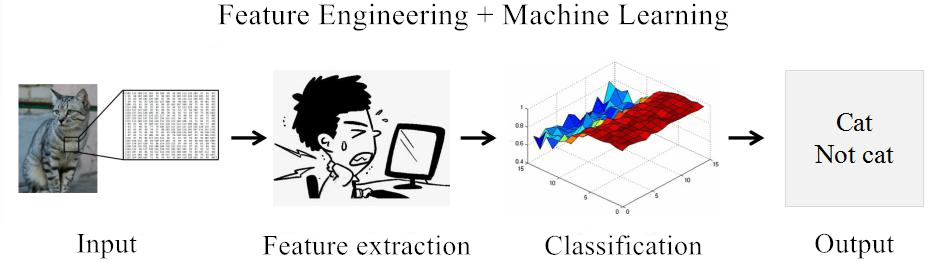
\includegraphics[width=8cm]{./Chapter5/Figures/feature-engineering.jpg}
    \end{minipage}%
    }
 \vfill
    \subfigure[端到端学习方法做图像分类]{
    \begin{minipage}{.9\textwidth}
        \centering
        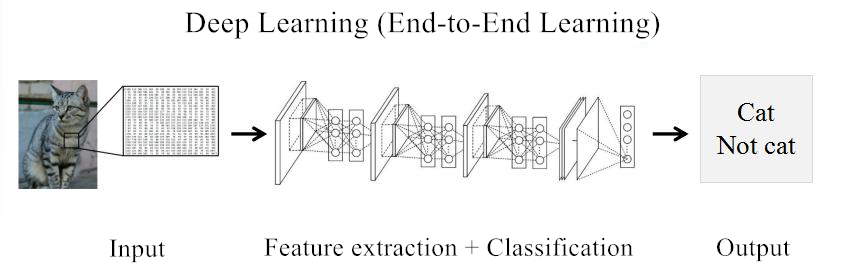
\includegraphics[width=8cm]{./Chapter5/Figures/deep-learning.jpg}
    \end{minipage}%
    }
\caption{特征工程{\small\sffamily\bfseries{vs}}端到端学习}
\label{fig:5-2}
\end {figure}
%------------------------------------------------------------------------------

\parinterval 传统的机器学习需要大量人工定义的特征,这些特征的构建往往会带来对问题的隐含假设。这种方法存在三方面的问题:

\begin{itemize}
\vspace{0.5em}
\item 特征的构造需要耗费大量的时间和精力。在传统机器学习的特征工程方法中,特征提取过程往往依赖于大量的先验假设,都基于人力完成的,这样导致相关系统的研发周期也大大增加;
\vspace{0.5em}
\item 最终的系统性能强弱非常依赖特征的选择。有一句话在业界广泛流传:``数据和特征决定了机器学习的上限'',但是人的智力和认知是有限的,因此人工设计的特征的准确性和覆盖度会受到限制;
\vspace{0.5em}
\item 通用性差。针对不同的任务,传统机器学习的特征工程方法需要选择出不同的特征,在这个任务上表现很好的特征在其他任务上可能没有效果。
\vspace{0.5em}
\end{itemize}

\parinterval 端到端学习将人们从大量的特征提取工作之中解放出来,可以不需要太多人的先验知识。从某种意义上讲,对问题的特征提取全是自动完成的,这也意味着哪怕我们不是该任务的``专家''也可以完成相关系统的开发。此外,端到端学习实际上也隐含了一种新的对问题的表示形式\ $\dash$\ {\small\bfnew{分布式表示}}\index{分布式表示}(Distributed Representation)\index{Distributed Representation}。在这种框架下,模型的输入可以被描述为分布式的实数向量,这样模型可以有更多的维度描述一个事物,同时避免传统符号系统对客观事物离散化的刻画。比如,在自然语言处理中,表示学习重新定义了什么是词,什么是句子。在本章后面的内容中也会看到,表示学习可以让计算机对语言文字的描述更加准确和充分。

%----------------------------------------------------------------------------------------
%    NEW SUBSUB-SECTION
%----------------------------------------------------------------------------------------

\subsubsection{深度学习的效果}

\parinterval 相比于传统的基于特征工程的方法,基于深度学习的模型更加方便、通用,在系统性能上也普遍更优。这里以语言建模任务为例。语言建模的目的是开发一个模型来描述词串出现的可能性(见第二章)。这个任务已经有着很长时间的历史。表\ref{tab:5-1}给出了不同方法在标准的PTB上的困惑度结果 \footnote{困惑度越低标明语言建模的效果越好。} 。传统的$ n$-gram语言模型由于面临维度灾难和数据稀疏问题,最终语言模型的性能并不是很好。而在深度学习模型中,通过引入循环神经网络等结构,所得到的语言模型可以更好地描述序列生成的问题。而最新的基于Transformer架构的语言模型将PPL从最初的178.0下降到了惊人的35.7。可见深度学习为这个任务所带来的进步是巨大的。

%----------------------------------------------------------------------------------------------------
\begin{table}[htp]
\centering
\caption{不同方法在PTB语言建模任务上的困惑度(PPL)}
\label{tab:5-1}
\small
\begin{tabular}{l | l l l}
\rule{0pt}{15pt}     模型 & 作者 & 年份 & PPL  \\
\hline
\rule{0pt}{15pt}     3-gram LM\cite{brown1992class} & Brown et al. & 1992 & 178.0  \\
\rule{0pt}{15pt}     Feed-forward Neural LM\cite{bengio2003neural} & Bengio et al. & 2003 & 162.2  \\
\rule{0pt}{15pt}     Recurrent NN-based LM\cite{mikolov2010recurrent} & Mikolov et al. & 2010 & 124.7  \\
\rule{0pt}{15pt}     Recurrent NN-LDA\cite{mikolov2012context} & Mikolov et al. & 2012 & 92.0  \\
\rule{0pt}{15pt}     LSTM \cite{zaremba2014recurrent}& Zaremba et al. & 2014 & 78.4  \\
\rule{0pt}{15pt}     RHN\cite{zilly2016recurrent} & Zilly et al. & 2016 & 65.4  \\
\rule{0pt}{15pt}     AWD-LSTM\cite{merity2017regularizing} & Merity et al. & 2018 & 58.8  \\
\rule{0pt}{15pt}     GPT-2 (Transformer)\cite{radford2019language} & Radford et al. & 2019 & 35.7  \\
\end{tabular}
\end{table}
%----------------------------------------------------------------------------------------------------

%----------------------------------------------------------------------------------------
%    NEW SECTION
%----------------------------------------------------------------------------------------

\sectionnewpage
\section{神经网络基础}

\parinterval 神经网络是一种由大量的节点(或称神经元)之间相互连接构成的计算模型。那么什么是神经元?神经元之间又是如何连接的?神经网络的数学描述又是什么样的?这一节将围绕这些问题对神经网络的基础知识进行系统的介绍。

%----------------------------------------------------------------------------------------
%    NEW SUB-SECTION
%----------------------------------------------------------------------------------------

\subsection{线性代数基础} \label{sec:5.2.1}

\parinterval 线性代数作为一个数学分支,广泛应用于科学和工程中,神经网络的数学描述中也大量使用了线性代数工具。因此,这里对线性代数的一些概念进行简要介绍,以方便后续对神经网络的数学建模。

%----------------------------------------------------------------------------------------
%    NEW SUBSUB-SECTION
%----------------------------------------------------------------------------------------

\subsubsection{标量、向量和矩阵}

\vspace{-0.5em}
\parinterval {\small\sffamily\bfseries{标量}}\index{标量}(Scalar)\index{Scalar}:标量亦称``无向量'',是一种只具有数值大小而没有方向的量,通俗地说,一个标量就是一个单独的数,这里特指实数\footnote{严格意义上,标量可以是复数等其他形式。这里为了方便讨论,仅以实数为对象。}。一般用小写斜体表示标量。比如,对于$ a=5 $,$ a $就是一个标量。

\parinterval {\small\sffamily\bfseries{向量}}\index{向量}(Vector)\index{Vector}:向量是由一组实数组成的有序数组。与标量不同,向量既有大小也有方向。可以把向量看作空间中的点,每个元素是不同坐标轴上的坐标。公式\ref{eq:5-1}和公式\ref{eq:5-2}展示了一个行向量和一个列向量。本章默认使用行向量,如$ \mathbf a=(a_1, a_2, a_3) $,$ \mathbf a $对应的列向量记为$ \mathbf a^{\rm T} $。
\begin{eqnarray}
\mathbf a &=& \begin{pmatrix}
  1 & 2 & 5 & 7
\end{pmatrix}\label{eq:5-1}\\ \nonumber \\
\mathbf{a^{\textrm{T}}} &=& \begin{pmatrix}
    &1& \\
    &2&\\
    &5& \\
    &7&\end{pmatrix}
\label{eq:5-2}
\end{eqnarray}

\parinterval {\small\sffamily\bfseries{矩阵}}\index{矩阵}(Matrix)\index{Matrix}:矩阵是一个按照长方阵列排列的实数集合,最早来自于方程组的系数及常数所构成的方阵。在计算机领域,通常将矩阵看作二维数组。我们用粗体的符号$ \mathbf a $表示一个矩阵,如果该矩阵有$ m $行$ n $列,那么有$ \mathbf a\in R^{m\times n} $。这里,用不加粗的符号来表示矩阵中的元素,其中每个元素都被一个行索引和一个列索引所确定。例如,$ a_{ij} $表示第$ i $行、第$ j $列的矩阵元素。如下,公式\ref{eq:5-3}中$ \mathbf a $定义了一个2行2列的矩阵。
\begin{eqnarray}
\mathbf a & = & \begin{pmatrix}
   a_{11} & a_{12}\\
   a_{21} & a_{22}
\end{pmatrix} \nonumber \\
& = & \begin{pmatrix}
   1 & 2\\
   3 & 4
\end{pmatrix}
\label{eq:5-3}
\end{eqnarray}

%----------------------------------------------------------------------------------------
%    NEW SUBSUB-SECTION
%----------------------------------------------------------------------------------------

\subsubsection{矩阵的转置}

\parinterval {\small\sffamily\bfseries{转置}}\index{转置}(Transpose)\index{Transpose}是矩阵的重要操作之一。矩阵的转置可以看作是将矩阵以对角线为镜像进行翻转:假设$ \mathbf a $为$ m $行$ n $列的矩阵,第$ i $行、第$ j $ 列的元素是$ a_{ij} $,即:$ \mathbf a={(a_{ij})}_{m\times n} $,把$ m\times n $矩阵$ \mathbf a $的行换成同序数的列得到一个$ n\times m $矩阵,则得到$ \mathbf a $的转置矩阵,记为$ \mathbf a^{\rm T} $,其中$ a_{ji}^{\rm T}=a_{ij} $。例如:
\begin{eqnarray}
\mathbf a & = & \begin{pmatrix} 1 & 3 & 2 & 6\\5 & 4 & 8 & 2\end{pmatrix} \\ \nonumber \\
{\mathbf a}^{\rm T} & = &\begin{pmatrix} 1 & 5\\3 & 4\\2 & 8\\6 & 2\end{pmatrix}
\end{eqnarray}

\parinterval 向量可以看作只有一行(列)的矩阵。对应地,向量的转置可以看作是只有一列(行)的矩阵。标量可以看作是只有一个元素的矩阵。因此,标量的转置等于它本身,即$ a^{\rm T}=a $。

%----------------------------------------------------------------------------------------
%    NEW SUBSUB-SECTION
%----------------------------------------------------------------------------------------

\subsubsection{矩阵加法和数乘}

\parinterval 矩阵加法又被称作{\small\sffamily\bfseries{按元素加法}}\index{按元素加法}(Element-wise Addition)\index{Element-wise Addition}。它是指两个矩阵把其相对应元素加在一起的运算,通常的矩阵加法被定义在两个形状相同的矩阵上。两个$ m\times n $矩阵$ \mathbf a $和$ \mathbf b $的和,标记为$ \mathbf a + \mathbf b $,它也是个$ m\times n $矩阵,其内的各元素为其相对应元素相加后的值。如果矩阵$ \mathbf c = \mathbf a + \mathbf b $,则$ c_{ij} = a_{ij} + b_{ij} $。公式\ref{eq:5-4}展示了矩阵之间进行加法的计算过程。
\begin{eqnarray}
\begin{pmatrix}
   1 & 3\\
   1 & 0\\
   1 & 2
\end{pmatrix}\;\;+\;\;\begin{pmatrix}
   0 & 0\\
   7 & 5\\
   2 & 1
\end{pmatrix}&=&\begin{pmatrix}
   1+0 & 3+0\\
   1+7 & 0+5\\
   1+2 & 2+1
\end{pmatrix}\;\;=\;\;\begin{pmatrix}
   1 & 3\\
   8 & 5\\
   3 & 3
\end{pmatrix}
\label{eq:5-4}
\end{eqnarray}

\parinterval 矩阵加法满足以下运算规律:

\begin{itemize}
\vspace{0.5em}
\item 交换律:$ \mathbf a+\mathbf b = \mathbf b +\mathbf a $。
\vspace{0.5em}
\item 结合律:$ (\mathbf a+\mathbf b)+\mathbf c = \mathbf a+(\mathbf b+\mathbf c) $。
\vspace{0.5em}
\item $ \mathbf a+\mathbf 0=\mathbf a $,其中$ \mathbf 0 $指的是零矩阵,即元素皆为0的矩阵。
\vspace{0.5em}
\item $ \mathbf a+(-\mathbf a)=\mathbf 0 $,其中$ -\mathbf a $是矩阵$ \mathbf a $的负矩阵,即将矩阵$ \mathbf a $的每个元素取负得到的矩阵。
\vspace{0.5em}
\end{itemize}

\parinterval 矩阵的{\small\bfnew{数乘}}\index{数乘}(Scalar Multiplication)\index{Scalar Multiplication}是指标量(实数)与矩阵的乘法运算,计算过程是将标量与矩阵的每个元素相乘,最终得到与原矩阵形状相同的矩阵。例如,矩阵$ \mathbf a={(a_{ij})}_{m\times n} $与标量$ k $进行数乘运算,其结果矩阵$ \mathbf b={(ka_{ij})}_{m\times n} $,即$ k{(a_{ij})}_{m\times n}={(ka_{ij})}_{m\times n} $。下面的式子展示了矩阵数乘的计算过程:
\begin{eqnarray}
\mathbf a & = &
\begin{pmatrix}
   3 & 2 & 7\\
   5 & 8 & 1
\end{pmatrix}
\\ \nonumber \\
2\mathbf a & = &
\begin{pmatrix}
   6 & 4 & 14\\
   10 & 16 & 2
\end{pmatrix}
\label{eq:5-5}
\end{eqnarray}

\parinterval 矩阵的数乘满足以下运算规律,其中$ k $和$ l $是实数,$ \mathbf a $和$ \mathbf b $是形状相同的矩阵:

\begin{itemize}
\vspace{0.5em}
\item 右分配律:$ k(\mathbf a+\mathbf b)=k\mathbf a+k\mathbf b $。
\vspace{0.5em}
\item 左分配律:$ (k+l)\mathbf a=k\mathbf a+l\mathbf a $。
\vspace{0.5em}
\item 结合律:$ (kl)\mathbf a=k(l\mathbf a) $。
%\vspace{0.5em}
\end{itemize}

%----------------------------------------------------------------------------------------
%    NEW SUBSUB-SECTION
%----------------------------------------------------------------------------------------

\subsubsection{矩阵乘法和矩阵点乘}

\parinterval 矩阵乘法是矩阵运算中最重要的操作之一,为了与矩阵点乘区分,通常也把矩阵乘法叫做矩阵叉乘。假设$ \mathbf a $为$ m\times p $的矩阵,$ \mathbf b $为$ p\times n $的矩阵,对$ \mathbf a $和$ \mathbf b $作矩阵乘法的结果是一个$ m\times n $的矩阵$ \mathbf c $,其中矩阵$ \mathbf c $中第$ i $行、第$ j $列的元素可以表示为:
\begin{eqnarray}
{(\mathbf a\mathbf b)}_{ij} &=& \sum_{k=1}^p a_{ik}b_{kj}
\label{eq:5-6}
\end{eqnarray}

\parinterval 只有当第一个矩阵的列数与第二个矩阵的行数相等时,两个矩阵才可以作矩阵乘法。公式\ref{eq:5-7}展示了矩阵乘法的运算过程,若$\mathbf a=\begin{pmatrix}a_{11} & a_{12}& a_{13}\\a_{21} & a_{22} & a_{23}\end{pmatrix}$,$\mathbf b=\begin{pmatrix}b_{11} & b_{12}\\b_{21} & b_{22}\\b_{31} & b_{32}\end{pmatrix} $,则有:
\vspace{-0.5em}
\begin{eqnarray}
\mathbf c & = & \mathbf a\mathbf b \nonumber \\
          & = & \begin{pmatrix}
   a_{11}b_{11}+a_{12}b_{21}+a_{13}b_{31} & a_{11}b_{12}+a_{12}b_{22}+a_{13}b_{32}\\
   a_{21}b_{11}+a_{22}b_{21}+a_{23}b_{31} & a_{21}b_{12}+a_{22}b_{22}+a_{23}b_{32}
\end{pmatrix}
\label{eq:5-7}
\end{eqnarray}

\parinterval 矩阵乘法满足以下运算规律:

\begin{itemize}
\vspace{0.5em}
\item 结合律:若$ \mathbf a\in R^{m\times n} $,$ \mathbf b\in R^{n\times p} $,$ \mathbf c\in R^{p\times q} $,则$ (\mathbf {ab})\mathbf c=\mathbf a(\mathbf {bc}) $。
\vspace{0.5em}
\item 左分配律:若$ \mathbf a\in R^{m\times n} $,$ \mathbf b\in R^{m\times n} $,$ \mathbf c\in R^{n\times p} $,则$ (\mathbf a+\mathbf b)\mathbf c=\mathbf {ac}+\mathbf {bc} $。
\vspace{0.5em}
\item 右分配律:若$ \mathbf a\in R^{m\times n} $,$ \mathbf b\in R^{n\times p} $,$ \mathbf c\in R^{n\times p} $,则$ \mathbf a(\mathbf b+\mathbf c)=\mathbf {ab}+\mathbf {ac} $。
\vspace{0.5em}
\end{itemize}

\begin{spacing}{1.4}
\parinterval 可以将线性方程组用矩阵乘法表示,如对于线性方程组$ \begin{cases} 5x_1+2x_2=y_1\\3x_1+x_2=y_2\end{cases} $,可以表示为$ \mathbf {ax}^{\rm T}=\mathbf y^{\rm T}$,其中$ \mathbf a = \begin{pmatrix} 5 & 2\\3 & 1\end{pmatrix} $,$ \mathbf x^{\rm T} = \begin{pmatrix} x_1\\x_2\end{pmatrix} $,$ \mathbf y^{\rm T} = \begin{pmatrix} y_1\\y_2\end{pmatrix} $。
\end{spacing}

\parinterval 矩阵的点乘就是两个形状相同的矩阵各个对应元素相乘,矩阵点乘也被称为{\small\bfnew{按元素乘积}}\index{按元素乘积}(Element-wise Product)\index{Element-wise Product}或Hadamard乘积,记为$ \mathbf a \odot \mathbf b$。例如,对于
\begin{eqnarray}
\mathbf a &=&
\begin{pmatrix}
   1 & 0\\
   -1 & 3
\end{pmatrix}
\\ \nonumber \\
\mathbf b &=&
\begin{pmatrix}
   3 & 1\\
   2 & 1
\end{pmatrix}
\end{eqnarray}

\parinterval 矩阵点乘的计算如下:
\begin{eqnarray}
\mathbf c & = & \mathbf a\odot \mathbf b \nonumber \\
          & = & \begin{pmatrix}
   1\times 3 & 0\times1\\
   -1\times2 & 3\times1
\end{pmatrix}
\label{eq:5-8}
\end{eqnarray}

%----------------------------------------------------------------------------------------
%    NEW SUBSUB-SECTION
%----------------------------------------------------------------------------------------

\subsubsection{线性映射}

\parinterval {\small\sffamily\bfseries{线性映射}}\index{线性映射}( Linear Mapping)\index{Linear Mapping}或{\small\sffamily\bfseries{线性变换}}\index{线性变换}(Linear Transformation)\index{Linear Transformation}是从一个向量空间V到另一个向量空间W的映射函数$ f:v\rightarrow w$,且该映射函数保持加法运算和数量乘法运算,即对于空间V中任何两个向量$ \mathbf u $ 和$ \mathbf v $以及任何标量$ c $,有:
\begin{eqnarray}
f(\mathbf u+\mathbf v)&=&f(\mathbf u)+f(\mathbf v)\label{eq:5-9}\\
f(c\mathbf v)&=&cf(\mathbf v)
\label{eq:5-10}
\end{eqnarray}

\parinterval 利用矩阵$ \mathbf a\in R^{m\times n} $,可以实现两个有限维欧氏空间的映射函数$f:R^n\rightarrow R^m$。例如$ n $维列向量$ \mathbf x ^{\rm T}$与$ m\times n $的矩阵$ \mathbf a $,向量$ \mathbf x ^{\rm T}$左乘矩阵$ \mathbf a $,可将向量$ \mathbf x ^{\rm T}$映射为$ m $列向量,对于
\begin{eqnarray}
\mathbf x^{\textrm{T}} & = & {\begin{pmatrix} x_1, & x_2, & \dots &, x_n \end{pmatrix}}^{\rm T}
\label{eq:5-11}
\end{eqnarray}

\begin{eqnarray}
\mathbf a&=&
\begin{pmatrix}
   a_{11} & a_{12} & \dots & a_{1n}\\
   a_{21} & \dots & \dots & \dots \\
   \dots & \dots & \dots & \dots \\
   a_{m1} & \dots & \dots & a_{mn}
\end{pmatrix}
\label{eq:5-12}
\end{eqnarray}

\parinterval 可以得到:
\begin{eqnarray}
\mathbf y^{\textrm{T}}& = &\mathbf a\mathbf x^{\textrm{T}} \nonumber \\
               & = &
\begin{pmatrix}
   a_{11}x_{1}+a_{12}x_{2}+\dots+a_{1n}x_{n}\\
   a_{21}x_{1}+a_{22}x_{2}+\dots+a_{2n}x_{n}\\
   \vdots \\
   a_{m1}x_{1}+a_{m2}x_{2}+\dots+a_{mn}x_{n}
\label{eq:5-13}\end{pmatrix}
\end{eqnarray}

\parinterval 上例中矩阵$ \mathbf a $定义了一个从$ R^n $到$ R^m $的线性映射:向量$ \mathbf x^{\textrm{T}}\in R^n $和$ \mathbf y^{\textrm{T}}\in R^m $别为两个空间中的列向量,即大小为$ n\times 1 $ 和$ m\times 1 $ 的矩阵。

%----------------------------------------------------------------------------------------
%    NEW SUBSUB-SECTION
%----------------------------------------------------------------------------------------

\subsubsection{范数}

\parinterval 工程领域,经常会使用被称为{\small\bfnew{范数}}\index{范数}(Norm)\index{Norm}的函数衡量向量大小,范数为向量空间内的所有向量赋予非零的正长度或大小。对于一个$n$维向量$ \mathbf x $,一个常见的范数函数为$ l_p $ 范数,通常表示为$ {\Vert{\mathbf x}\Vert}_p $ ,其中$p\ge 0$,是一个标量形式的参数。常用的$ p $的取值有$ 1 $、$ 2 $、$ \infty $等。范数的计算公式为:
\begin{eqnarray}
l_p(\mathbf x) & = & {\Vert{\mathbf x}\Vert}_p \nonumber \\
               & = & {\left (\sum_{i=1}^{n}{{\vert x_{i}\vert}^p}\right )}^{\frac{1}{p}}
\label{eq:5-14}
\end{eqnarray}

\parinterval $ l_1 $范数为向量的各个元素的绝对值之和:
\begin{eqnarray}
{\Vert{\mathbf x}\Vert}_1&=&\sum_{i=1}^{n}{\vert x_{i}\vert}
\label{eq:5-15}
\end{eqnarray}

\parinterval $ l_2 $范数为向量的各个元素平方和的二分之一次方:
\begin{eqnarray}
{\Vert{\mathbf x}\Vert}_2&=&\sqrt{\sum_{i=1}^{n}{{x_{i}}^2}} \nonumber \\
                                      &=&\sqrt{{\mathbf x}^{\rm T}\mathbf x}
\label{eq:5-16}
\end{eqnarray}

\parinterval $ l_2 $范数被称为{\small\bfnew{欧几里得范数}}\index{欧几里得范数}(Euclidean Norm)\index{Euclidean Norm}。从几何角度,向量也可以表示为从原点出发的一个带箭头的有向线段,其$ l_2 $范数为线段的长度,也常被称为向量的模。$ l_2 $ 范数在机器学习中非常常用,向量$ \mathbf x $的$ l_2 $范数经常简化为$ \Vert{\mathbf x}\Vert $,可以简单地通过点积$ {\mathbf x}^{\rm T}\mathbf x $计算。

\parinterval $ l_{\infty} $范数为向量的各个元素的最大绝对值:
\begin{eqnarray}
{\Vert{\mathbf x}\Vert}_{\infty}&=&{\rm{max}}\{x_1,x_2,\dots,x_n\}
\label{eq:5-17}
\end{eqnarray}

\parinterval 广义上讲,范数是将向量映射到非负值的函数,其作用是衡量向量$ \mathbf x $到坐标原点的距离。更严格的说,范数并不拘于$ l_p $范数,任何一个同时满足下列性质的函数都可以作为范数:

\begin{itemize}
\vspace{0.5em}
\item 若$ f(x)=0 $,则$ x=0 $。
\vspace{0.5em}
\item 三角不等式:$ f(x+y)\leqslant f(x)+f(y) $。
\vspace{0.5em}
\item 任意实数$ \alpha $,$ f(\alpha x)=\vert \alpha \vert f(x) $。
\vspace{0.5em}
\end{itemize}

\parinterval 在深度学习中,有时候希望衡量矩阵的大小,这时可以考虑使用 {\small\bfnew{Frobenius 范数}}\index{Frobenius 范数}(Frobenius Norm)\index{Frobenius Norm}。计算方式为:
\begin{eqnarray}
{\Vert{\mathbf a}\Vert}_F&=&\sqrt{\sum_{i,j} a_{i,j}^2}
\label{eq:5-18}
\end{eqnarray}

%----------------------------------------------------------------------------------------
%    NEW SUB-SECTION
%----------------------------------------------------------------------------------------
\subsection{人工神经元和感知机}

\parinterval 生物学中,神经元是神经系统的基本组成单元。图\ref{fig:5-3}展示了一个生物神经元实例。

%----------------------------------------------
\begin{figure}[htp]
\centering
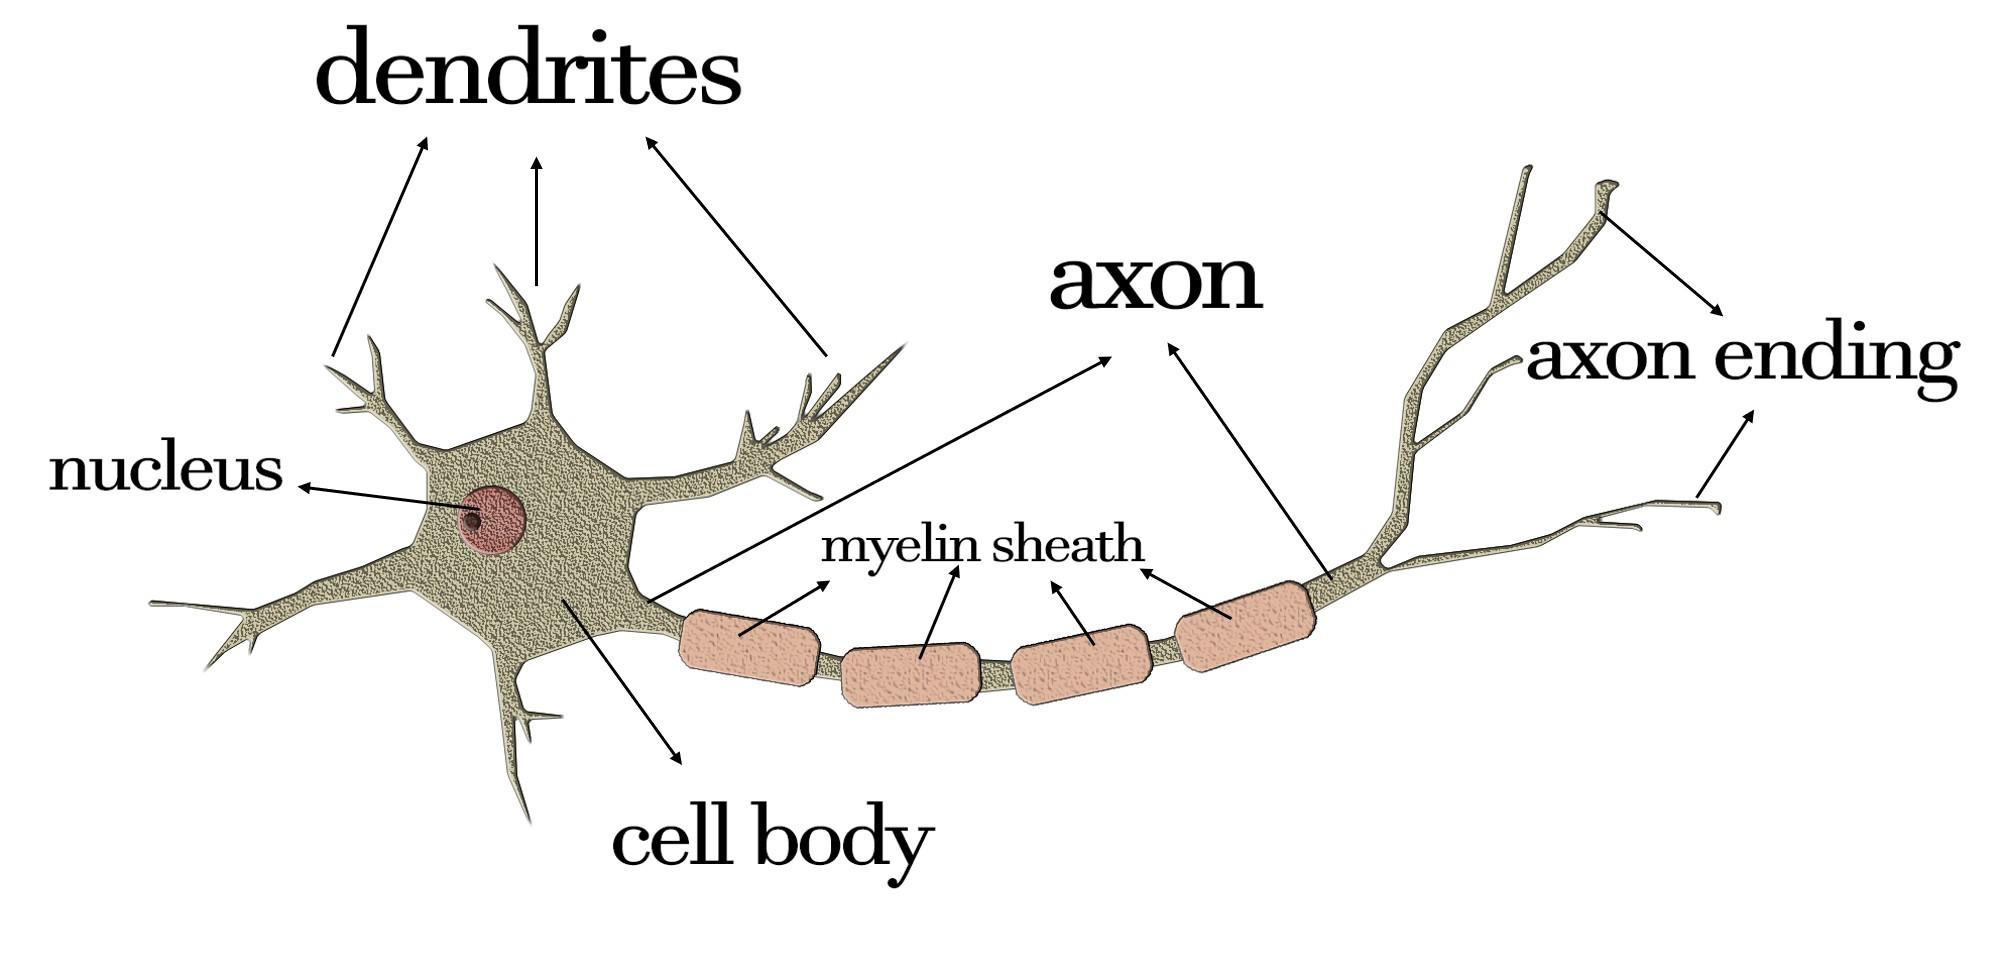
\includegraphics[width=8cm]{./Chapter5/Figures/biological-neuron.jpg}
\caption{生物神经元}
\label{fig:5-3}
\end{figure}
%-------------------------------------------

\parinterval 同样,人工神经元是人工神经网络的基本单元。在人们的想象中,人工神经元应该与生物神经元类似。但事实上,二者在形态上是有明显差别的。如图\ref{fig:5-4} 是一个典型的人工神经元,其本质是一个形似$ y=f(\mathbf x\cdot \mathbf w+b) $的函数。显而易见,一个神经元主要由$ \mathbf x $,$ \mathbf w $,$ b $,$ f $四个部分构成。其中$ \mathbf x $是一个形如$ (x_0,x_1,\dots,x_n) $ 的实数向量,在一个神经元中担任``输入''的角色。$ \mathbf w $是一个权重矩阵,其中的每一个元素都对应着一个输入和一个输出,代表着``某输入对某输出的贡献程度'',通常也被理解为神经元连接的{\small\sffamily\bfseries{权重}}\index{权重}(weight)\index{weight}。$ b $被称作偏置,是一个实数。$ f $被称作激活函数,其本质是一个非线性函数。可见,一个人工神经元的功能是将输入向量与权重矩阵右乘(做内积)后,加上偏置量,经过一个非线性激活函数得到一个标量结果。

%----------------------------------------------
\begin{figure}[htp]
\centering
%%%------------------------------------------------------------------------------------------------------------
\begin{tikzpicture}
\begin{scope}
\node [anchor=center,circle,draw,ublue,very thick,minimum size=3.5em,fill=white,drop shadow={shadow xshift=0.1em,shadow yshift=-0.1em}] (neuron) at (0,0) {};
\node [anchor=east] (x1) at ([xshift=-6em]neuron.west) {\Large{$x_1$}};
\node [anchor=center] (x0) at ([yshift=3em]x1.center) {\Large{$x_0$}};
\node [anchor=center] (x2) at ([yshift=-3em]x1.center) {\Large{$b$}};
\node [anchor=west] (y) at ([xshift=6em]neuron.east) {\Large{$y$}};
\node [anchor=center] (neuronmath) at (neuron.center) {\Large{$f$}};

\draw [->,thick] (x0.east) -- (neuron.150) node [pos=0.5,above] {$w_0$};
\draw [->,thick] (x1.east) -- (neuron.180) node [pos=0.5,above] {$w_1$};
\draw [->,thick] (x2.east) -- (neuron.210) node [pos=0.5,above] {$$};
\draw [->,thick] (neuron.east) -- (y.west);

\end{scope}
\end{tikzpicture}
%
%%%------------------------------------------------------------------------------------------------------------


\caption{人工神经元}
\label{fig:5-4}
\end{figure}
%----------------------------------------------

%----------------------------------------------------------------------------------------
%    NEW SUBSUB-SECTION
%----------------------------------------------------------------------------------------

\vspace{-0.5em}
\subsubsection{感知机\ \dash \ 最简单的人工神经元模型}

\vspace{0.5em}
\parinterval 感知机是人工神经元的一种实例,在上世纪50-60年代被提出后,对神经网络研究产生了深远的影响。感知机模型如图\ref {fig:5-5}所示,其输入是一个$n$维二值向量$ \mathbf x=(x_0,x_1,\dots,x_n) $,其中$ x_i=0 $或$ 1 $。权重$ \mathbf w=(w_0,w_1,\dots,w_n) $,每个输入变量对应一个权重$ w_i $(实数)。偏置$ b $是一个实数变量($ -\sigma $)。输出也是一个二值结果,即$ y=0 $或$ 1 $。$ y $值的判定由输入的加权和是否大于(或小于)一个阈值$ \sigma $决定(公式\ref{eq:5-19}):
\begin{eqnarray}
y=\begin{cases} 0 & \sum_{i}{x_i\cdot w_i}-\sigma <0\\1 & \sum_{i}{x_i\cdot w_i}-\sigma \geqslant 0\end{cases}
\label{eq:5-19}
\end{eqnarray}

%----------------------------------------------
\begin{figure}[htp]
\centering
%%%------------------------------------------------------------------------------------------------------------
 \begin{tikzpicture}
\begin{scope}
\node [anchor=center,circle,draw,ublue,very thick,minimum size=3.5em,fill=white,drop shadow={shadow xshift=0.1em,shadow yshift=-0.1em}] (neuron) at (0,0) {};
\node [anchor=east] (x1) at ([xshift=-6em]neuron.west) {\Large{$x_1$}};
\node [anchor=center] (x0) at ([yshift=3em]x1.center) {\Large{$x_0$}};
\node [anchor=center] (x2) at ([yshift=-3em]x1.center) {\Large{$x_2$}};
\node [anchor=west] (y) at ([xshift=6em]neuron.east) {\Large{$y$}};
\node [anchor=center] (neuronmath) at (neuron.center) {\red{\small{$\sum \ge \sigma$}}};

\draw [->,thick] (x0.east) -- (neuron.150) node [pos=0.5,above] {$w_0$};
\draw [->,thick] (x1.east) -- (neuron.180) node [pos=0.5,above] {$w_1$};
\draw [->,thick] (x2.east) -- (neuron.210) node [pos=0.5,above] {$w_2$};
\draw [->,thick] (neuron.east) -- (y.west);

\end{scope}
\end{tikzpicture}
%%%------------------------------------------------------------------------------------------------------------


\caption{感知机模型}
\label{fig:5-5}
\end{figure}
%-------------------------------------------

\parinterval 感知机可以做一些简单的决策。举一个非常简单的例子,有一场音乐会,你正在纠结是否去参加,有三个因素会影响你的决定:

\begin{itemize}
\vspace{0.5em}
\item $ x_0 $:剧场是否离你足够近(是,则$ x_0=1 $;否则$ x_0=0 $);
\vspace{0.5em}
\item $ x_1 $:票价是否低于300元(是,则$ x_1=1 $;否则$ x_1=0 $);
\vspace{0.5em}
\item $ x_2 $:女朋友是否喜欢音乐会(是,则$ x_2=1 $;否则$ x_2=0 $)。
\vspace{0.5em}
\end{itemize}

\parinterval 在这种情况下应该如何做出决定呢?比如,女朋友很希望和你一起去看音乐会,但是剧场很远而且票价500元,如果这些因素对你都是同等重要的(即$ w_0=w_1=w_2 $,假设这三个权重都设置为1)那么会得到一个综合得分:
\begin{eqnarray}
x_0\cdot w_0+x_1\cdot w_1+x_2\cdot w_2 & = & 0\cdot 1+0\cdot 1+1\cdot 1 \nonumber \\
                                                                     & = & 1
\label{eq:5-20}
\end{eqnarray}

\parinterval 如果你不是十分纠结的人,能够接受不完美的事情,你可能会把$ \sigma $设置为1,于是$ \sum{w_i\cdot x_i}-\sigma \ge 0 $,那么你会去音乐会。可以看出,上面的例子的本质就是一个如图\ref{fig:5-6}的感知机:

%----------------------------------------------
\begin{figure}[htp]
\centering
%%%------------------------------------------------------------------------------------------------------------
 \begin{tikzpicture}
\begin{scope}
\node [anchor=center,circle,draw,ublue,very thick,minimum size=3.5em,fill=white,drop shadow={shadow xshift=0.1em,shadow yshift=-0.1em}] (neuron) at (0,0) {};
\node [anchor=east] (x1) at ([xshift=-6em]neuron.west) {$x_1$:票价够低?};
\node [anchor=center] (x0) at ([yshift=3em]x1.center) {$x_0$:距离够近?};
\node [anchor=center] (x2) at ([yshift=-3em]x1.center) {$x_2$:女友喜欢?};
\node [anchor=west] (y) at ([xshift=2em]neuron.east) {$y$:去?还是不去?};

{
\draw [->,thick] (x0.east) -- (neuron.150) node [pos=0.5,above,yshift=0.2em] {\small{$w_0=1$}};
\draw [->,thick] (x1.east) -- (neuron.180) node [pos=0.5,above,yshift=-0.1em] {\small{$w_1=1$}};
\draw [->,thick] (x2.east) -- (neuron.210) node [pos=0.5,above,yshift=0.1em] {\small{$w_2=1$}};
}
\draw [->,thick] (neuron.east) -- (y.west);

\node [anchor=center] (neuronmath) at (neuron.center) {\small{$\sum \ge \sigma$}};

\end{scope}
\end{tikzpicture}
%%%------------------------------------------------------------------------------------------------------------



\caption{预测是否去剧场的感知机(权重相同)}
\label{fig:5-6}
\end{figure}
%-------------------------------------------

%----------------------------------------------------------------------------------------
%    NEW SUBSUB-SECTION
%----------------------------------------------------------------------------------------

\vspace{-1em}
\subsubsection{神经元内部权重}

\parinterval 在上面的例子中,连接权重代表着每个输入因素对最终输出结果的重要程度,为了得到令人满意的决策,需要不断调整权重。如果你是守财奴,则会对票价看得更重一些,这样你会用不均匀的权重计算每个因素的影响,比如:$ w_0=0.5 $,$ w_1=2 $,$ w_2=0.5 $,此时感知机模型如图\ref{fig:5-7}所示。在这种情况下,女友很希望和你一起去看音乐会,但是剧场很远而且票价500元,会导致你不去看音乐会,因为
\begin{eqnarray}
\sum_{i}{x_i\cdot w_i} & = & 0\cdot 0.5+0\cdot 2+1\cdot 0.5 \nonumber \\
                                   & = & 0.5 \nonumber \\
                                   & < & \sigma = 1
\label{eq:5-21}
\end{eqnarray}

%----------------------------------------------
\begin{figure}[htp]
\centering
%%%------------------------------------------------------------------------------------------------------------
\begin{tikzpicture}
\begin{scope}
\node [anchor=center,circle,draw,ublue,very thick,minimum size=3.5em,fill=white,drop shadow={shadow xshift=0.1em,shadow yshift=-0.1em}] (neuron) at (0,0) {};
\node [anchor=east] (x1) at ([xshift=-6em]neuron.west) {$x_1$:票价够低?};
\node [anchor=center] (x0) at ([yshift=3em]x1.center) {$x_0$:距离够近?};
\node [anchor=center] (x2) at ([yshift=-3em]x1.center) {$x_2$:女友喜欢?};
\node [anchor=west] (y) at ([xshift=2em]neuron.east) {$y$:去?还是不去?};


\draw [->,thin] (x0.east) -- (neuron.150) node [pos=0.5,above,yshift=0.2em] {\small{$w_0=.5$}};
\draw [->,line width=0.5mm] (x1.east) -- (neuron.180) node [pos=0.5,above,yshift=-0.1em] {\textbf{\small{$w_1=2$}}};
\draw [->,thin] (x2.east) -- (neuron.210) node [pos=0.5,above,yshift=0.1em] {\small{$w_2=.5$}};
\draw [->,thick] (neuron.east) -- (y.west);

\node [anchor=center] (neuronmath) at (neuron.center) {\small{$\sum \ge \sigma$}};
\node [anchor=south] (ylabel) at (y.north) {\textbf{不去了!}};


\end{scope}
\end{tikzpicture}
%%%------------------------------------------------------------------------------------------------------------



\caption{预测是否去剧场的感知机(改变权重)}
\label{fig:5-7}
\end{figure}
%-------------------------------------------

\parinterval 当然,结果是女友对这个决定非常不满意,让你跪键盘上反思一下自己。

%----------------------------------------------------------------------------------------
%    NEW SUBSUB-SECTION
%----------------------------------------------------------------------------------------

\subsubsection{神经元的输入\ \dash \ 离散 vs 连续}

\parinterval 在遭受了女友一万点伤害之后,你意识到决策考虑的因素(即输入)不应该只是非0即1,而应该把``程度''考虑进来,于是你改变了三个输入的形式:

\parinterval $ x_0 $:10/距离

\parinterval $ x_1 $:150/票价

\parinterval $ x_2 $:女朋友是否喜欢

\parinterval 在新修改的模型中,$ x_0 $和$ x_1 $变成了连续变量,$ x_2 $仍然是离散变量,如图\ref{fig:5-8}。

%----------------------------------------------
\begin{figure}[htp]
\centering
%%%------------------------------------------------------------------------------------------------------------
\begin{tikzpicture}

\begin{scope}
\draw [->,thick] (0,0) -- (2.5,0);
\draw [->,thick] (0,0) -- (0, 1.5);
\draw [-,very thick,ublue,domain=0.6:2,samples=100] plot (\x,{ 1/\x - 0.2});
\node [anchor=east] (ylabel) at (0, 3.2em) {\footnotesize{$x_0$}};
\node [anchor=north] (xlabel) at (5em, 0em) {\scriptsize{距离(km)}};
\end{scope}

\begin{scope}[xshift=9em]
\draw [->,thick] (0,0) -- (2.5,0);
\draw [->,thick] (0,0) -- (0, 1.5);
\draw [-,very thick,ublue,domain=0.4:2,samples=100] plot (\x,{ 0.5/\x});
\node [anchor=east] (ylabel) at (0, 3.2em) {\footnotesize{$x_1$}};
\node [anchor=north] (xlabel) at (5em, 0em) {\scriptsize{票价(元)}};
\end{scope}

\begin{scope}[xshift=18em]
\draw [->,thick] (0,0) -- (2.5,0);
\draw [->,thick] (0,0) -- (0, 1.5);
\node [anchor=east] (ylabel) at (0, 3.2em) {\footnotesize{$x_2$}};
\node [anchor=south, fill=ublue, minimum width=1.5em, minimum height=0.1em, inner sep=0] (histogram1) at (1.5em, 0) {};
\node [anchor=south, fill=ublue, minimum width=1.5em, minimum height=3em, inner sep=0] (histogram2) at (4.0em, 0) {};
\node [anchor=north] (hlabel1) at (histogram1.south) {\tiny{女友不去}};
\node [anchor=north] (hlabel2) at (histogram2.south) {\tiny{女友去}};
\end{scope}

\end{tikzpicture}
%%%------------------------------------------------------------------------------------------------------------



\caption{神经元输入的不同形式}
\label{fig:5-8}
\end{figure}
%-------------------------------------------

\parinterval 使用修改后的模型做决策:女朋友很希望和你一起,但是剧场有20km远而且票价有500元。于是有$ x_0=10/20 $,$ x_1=150/500 $,$ x_2=1 $。
\begin{eqnarray}
\sum_{i}{x_i\cdot w_i} & = & 0.5\cdot 0.5+0.3\cdot 2+1\cdot 0.5 \nonumber \\
                                   & = & 1.35 \nonumber \\
                                   & > & \sigma =1
\label{eq:5-22}
\end{eqnarray}

\parinterval 虽然剧场很远,价格有点贵,但是女友很满意,你还是很高兴。

%----------------------------------------------------------------------------------------
%    NEW SUBSUB-SECTION
%----------------------------------------------------------------------------------------

\subsubsection{神经元内部的参数学习}

\parinterval 一次成功的音乐会之后,你似乎掌握了一个真理:其他什么都不重要,女友的喜好最重要,所以你又将决策模型的权重做出了调整:最简单的方式就是$ w_0=w_1=0 $,同时令$ w_2>0 $,相当于只考虑$ x_2 $的影响而忽略其他因素,于是你得到了如图\ref {fig:5-9}所示的决策模型:

%----------------------------------------------
\begin{figure}[htp]
\centering
%%%------------------------------------------------------------------------------------------------------------
\begin{tikzpicture}
\begin{scope}
\node [anchor=center,circle,draw,ublue,very thick,minimum size=3.5em,fill=white,drop shadow={shadow xshift=0.1em,shadow yshift=-0.1em}] (neuron) at (0,0) {};
\node [anchor=east] (x1) at ([xshift=-6em]neuron.west) {$x_1$:便宜程度\ \ \ \ };
\node [anchor=center] (x0) at ([yshift=3em]x1.center) {$x_0$:远近程度\ \ \ \ };
\node [anchor=center] (x2) at ([yshift=-3em]x1.center) {$x_2$:女友喜欢?};
\node [anchor=west] (y) at ([xshift=2em]neuron.east) {$y$:去?还是不去?};

\draw [->,thick] (neuron.east) -- (y.west);

\node [anchor=center] (neuronmath) at (neuron.center) {\small{$\sum \ge \sigma$}};

{
\draw [->,dotted] (x0.east) -- (neuron.150) node [pos=0.5,above,yshift=0.2em] {\small{$w_0=0$}};
\draw [->,dotted] (x1.east) -- (neuron.180) node [pos=0.5,above,yshift=-0.1em] {\textbf{\small{$w_1=0$}}};
\draw [->,line width=0.5mm] (x2.east) -- (neuron.210) node [pos=0.5,above,yshift=0.1em] {\small{$w_2=10$}};
}


\end{scope}
\end{tikzpicture}
%%%------------------------------------------------------------------------------------------------------------



\caption{预测是否去剧场的决策模型(只考虑女友喜好)}
\label{fig:5-9}
\end{figure}
%-------------------------------------------

\parinterval 很快又有了一场音乐会,距你1000公里,票价3000元,当然女友是一直喜欢音乐会的。根据新的决策模型,你义无反顾地选择去看音乐会。然而,女友又不高兴了,喜欢浪漫的女友觉得去看这场音乐会太奢侈了。在这几次看音乐会的经历中,你发现每个因素的权重需要准确地设置才能达到最好的决策效果。

\parinterval 那么如何确定最好的权重的?方法其实很简单,不断地尝试,根据结果不断地调整权重。在经过成百上千次的尝试之后,终于找到了一组合适的权重,使每次决策的正确率都很高。上面这个过程就类似于参数训练的过程,利用大量的数据来模拟成百上千次的尝试,根据输出的结果来不断地调整权重。

\parinterval 可以看到,在``是否参加音乐会''这个实际问题中,主要涉及到三方面的问题:

\begin{itemize}
\vspace{0.5em}
\item 对问题建模,即定义输入$ \{x_i\} $的形式;
\vspace{0.5em}
\item 设计有效的决策模型,即定义$ y $;
\vspace{0.5em}
\item 决定模型所涉及的参数(如权重$ \{w_i\} $)的最优值。
\vspace{0.5em}
\end{itemize}

\parinterval 上面的例子对这三个问题都简要地做出了回答。下面的内容将继续对它们进行详细阐述。

%----------------------------------------------------------------------------------------
%    NEW SUB-SECTION
%----------------------------------------------------------------------------------------

\subsection{多层神经网络}

\parinterval 感知机是一种最简单的单层神经网络。一个非常自然的问题是:能否把多个这样的网络叠加在一起,获得建模更复杂问题的能力?如果可以,那么在多层神经网络的每一层,神经元之间是怎么组织、工作的呢?单层网络又是通过什么方式构造成多层的呢?

%----------------------------------------------------------------------------------------
%    NEW SUBSUB-SECTION
%----------------------------------------------------------------------------------------

\subsubsection{线性变换和激活函数}

\parinterval 为了建立多层神经网络,首先需要把前面提到的简单的神经元进行扩展,把多个神经元组成一``层''神经元。比如,很多实际问题需要同时有多个输出,这时可以把多个相同的神经元并列起来,每个神经元都会有一个单独的输出,这就构成一``层'',形成了单层神经网络。单层神经网络中的每一个神经元都对应着一组权重和一个输出,可以把单层神经网络中的不同输出看作一个事物不同角度的描述。

%----------------------------------------------
\begin{figure}[htp]
\centering
%%%------------------------------------------------------------------------------------------------------------
\begin{tikzpicture}
\begin{scope}

\tikzstyle{neuronnode} = [minimum size=1.5em,circle,draw,ublue,very thick,fill=white,drop shadow={shadow xshift=0.1em,shadow yshift=-0.1em}]

\node [anchor=center,neuronnode] (neuron00) at (0,0) {};
\node [anchor=center,neuronnode] (neuron01) at ([yshift=-3em]neuron00) {};
\node [anchor=center,neuronnode] (neuron02) at ([yshift=-3em]neuron01) {};

\node [anchor=east] (x0) at ([xshift=-6em]neuron00.west) {$x_0$};
\node [anchor=east] (x1) at ([xshift=-6em]neuron01.west) {$x_1$};
\node [anchor=east] (x2) at ([xshift=-6em]neuron02.west) {$b$};

\node [anchor=west] (y0) at ([xshift=4em]neuron00.east) {$y_0$:\scriptsize{温度}};

\draw [->,red!50,line width=0.4mm] (x0.east) -- (neuron00.180) node [pos=0.1,above] {\tiny{$w_{00}$}};
\draw [->,red!50,line width=0.4mm] (x1.east) -- (neuron00.200) node [pos=0.1,above] {\tiny{$w_{10}$}};
\draw [->,red!50,line width=0.4mm] (x2.east) -- (neuron00.220) node [pos=0.05,above,yshift=0.3em] {\tiny{$b_{0}$}};
\draw [->,red!30,line width=0.4mm] (neuron00.east) -- (y0.west);

\node [anchor=west] (y1) at ([xshift=4em]neuron01.east) {$y_1$:\scriptsize{湿度}};

\draw [->,blue!50,line width=0.4mm] (x0.east) -- (neuron01.160) node [pos=0.4,above] {\tiny{$w_{01}$}};
\draw [->,blue!50,line width=0.4mm] (x1.east) -- (neuron01.180) node [pos=0.35,above,yshift=-0.2em] {\tiny{$w_{11}$}};
\draw [->,blue!50,line width=0.4mm] (x2.east) -- (neuron01.200) node [pos=0.3,below,yshift=0.2em] {\tiny{$b_{1}$}};
\draw [->,blue!30,line width=0.4mm] (neuron01.east) -- (y1.west);

\node [anchor=west] (y2) at ([xshift=4em]neuron02.east) {$y_2$:\scriptsize{风力}};

\draw [->,purple!40,line width=0.4mm] (x0.east) -- (neuron02.140) node [pos=0.1,below,yshift=-0.2em] {\tiny{$w_{02}$}};
\draw [->,purple!40,line width=0.4mm] (x1.east) -- (neuron02.160) node [pos=0.1,below] {\tiny{$w_{12}$}};
\draw [->,purple!40,line width=0.4mm] (x2.east) -- (neuron02.180) node [pos=0.3,below] {\tiny{$b_{2}$}};
\draw [->,purple!30,line width=0.4mm] (neuron02.east) -- (y2.west);

\end{scope}
\end{tikzpicture}



%%%------------------------------------------------------------------------------------------------------------


\caption{权重矩阵中的元素与输出的对应关系}
\label{fig:5-10}
\end{figure}
%-------------------------------------------

\parinterval 举个简单的例子,预报天气时,往往需要预测温度、湿度和风力,这就意味着如果使用单层神经网络进行预测,需要设置3个神经元。如图\ref{fig:5-10},权重矩阵为:
\begin{eqnarray}
\mathbf w=\begin{pmatrix} w_{00} & w_{01} & w_{02}\\ w_{10} & w_{11} & w_{12}\end{pmatrix}
\end{eqnarray}

\noindent 它的第一列元素$ \begin{pmatrix} w_{00}\\ w_{10}\end{pmatrix} $是输入相对第一个输出$ y_0 $ 的权重,参数向量$ \mathbf b=(b_0,b_1,b_2) $的第一个元素$ b_0 $是对应于第一个输出$ y_0 $ 的偏置量;类似的,可以得到$ y_1 $和$ y_2 $。预测天气的单层模型如图\ref{fig:5-11}所示(在本例中,假设输入$ \mathbf x=(x_0,x_1) $)。

%----------------------------------------------
\begin{figure}[htp]
\centering
%%%------------------------------------------------------------------------------------------------------------
\begin{tikzpicture}
\begin{scope}

\tikzstyle{neuronnode} = [minimum size=1.5em,circle,draw,ublue,very thick,fill=white,drop shadow={shadow xshift=0.1em,shadow yshift=-0.1em}]

\node [anchor=center,neuronnode] (neuron00) at (0,0) {};
\node [anchor=center,neuronnode] (neuron01) at ([yshift=-3em]neuron00) {};
\node [anchor=center,neuronnode] (neuron02) at ([yshift=-3em]neuron01) {};
\node [anchor=east] (x0) at ([xshift=-6em]neuron00.west) {$x_0$};
\node [anchor=east] (x1) at ([xshift=-6em]neuron01.west) {$x_1$};
\node [anchor=east] (x2) at ([xshift=-6em]neuron02.west) {$b$};
\node [anchor=west] (y0) at ([xshift=4em]neuron00.east) {$y_0$};

\draw [->] (x0.east) -- (neuron00.180) node [pos=0.1,above] {\tiny{$w_{00}$}};
\draw [->] (x1.east) -- (neuron00.200) node [pos=0.1,above] {\tiny{$w_{10}$}};
\draw [->] (x2.east) -- (neuron00.220) node [pos=0.05,above,yshift=0.3em] {\tiny{$b_{0}$}};
\draw [->] (neuron00.east) -- (y0.west);

\node [anchor=west] (y1) at ([xshift=4em]neuron01.east) {$y_1$};
\draw [->] (x0.east) -- (neuron01.160) node [pos=0.4,above] {\tiny{$w_{01}$}};
\draw [->] (x1.east) -- (neuron01.180) node [pos=0.35,above,yshift=-0.2em] {\tiny{$w_{11}$}};
\draw [->] (x2.east) -- (neuron01.200) node [pos=0.3,below,yshift=0.2em] {\tiny{$b_{1}$}};
\draw [->] (neuron01.east) -- (y1.west);

\node [anchor=west] (y2) at ([xshift=4em]neuron02.east) {$y_2$};
\draw [->] (x0.east) -- (neuron02.140) node [pos=0.1,below,yshift=-0.2em] {\tiny{$w_{02}$}};
\draw [->] (x1.east) -- (neuron02.160) node [pos=0.1,below] {\tiny{$w_{12}$}};
\draw [->] (x2.east) -- (neuron02.180) node [pos=0.3,below] {\tiny{$b_{2}$}};
\draw [->] (neuron02.east) -- (y2.west);

\node [anchor=east,align=left] (inputlabel) at ([xshift=-0.1em]x1.west) {\scriptsize{输入向量}:\\\small{$\textbf{x}=(x_0,x_1)$}};


\node [anchor=west,align=left] (outputlabel) at ([xshift=0.1em]y1.east) {\scriptsize{输出向量}:\\\small{$\textbf{y}=(y_0,y_1,y_2)$}};


\begin{pgfonlayer}{background}

\node [rectangle,inner sep=0.4em,fill=red!20] [fit = (neuron00) (neuron01) (neuron02)] (layer) {};
\node [anchor=south] (layerlabel) at ([yshift=0.2em]layer.north) {\scriptsize{一层神经元}};



\node [rectangle,inner sep=0.1em,fill=ugreen!20] [fit = (x0) (x1)] (inputshadow) {};


\node [rectangle,inner sep=0.1em,fill=blue!20] [fit = (y0) (y1) (y2)] (outputshadow) {};

\end{pgfonlayer}



\end{scope}
\end{tikzpicture}
%%%------------------------------------------------------------------------------------------------------------


\caption{预测天气的单层神经网络}
\label{fig:5-11}
\end{figure}
%-------------------------------------------

\parinterval 在神经网络中,对于输入向量$ \mathbf x\in R^m $,一层神经网络首先将其经过线性变换映射到$ R^n $,再经过激活函数变成$  \mathbf y\in R^n $。还是上面天气预测的例子,每个神经元获得相同的输入,权重矩阵$ \mathbf w $是一个$ 2\times 3 $矩阵,矩阵中每个元素$ w_{ij} $代表第$ j $个神经元中$ x_{i} $对应的权重值,假设编号为0的神经元负责预测温度,则$ w_{i0} $含义为预测温度时,输入$ x_{i} $对其影响程度。此外所有神经元的偏置$ b_{0} $,$ b_{1} $,$ b_{2} $组成了最终的偏置向量$ \mathbf b $。在该例中则有,权重矩阵$ \mathbf w=\begin{pmatrix} w_{00} & w_{01} & w_{02}\\ w_{10} & w_{11} & w_{12}\end{pmatrix} $,偏置向量$ \mathbf b=(b_0,b_1,b_2) $。

%----------------------------------------------
\begin{figure}[htp]
\centering
%%%------------------------------------------------------------------------------------------------------------
\begin{tikzpicture}

\tikzstyle{neuron} = [rectangle,draw,thick,fill=red!30,red!35,minimum height=2em,minimum width=2em,font=\small]
\node[neuron,anchor=north] (a1) at (0,0) {};
\draw[->,thick] ([xshift=-2em,yshift=0em]a1.south) to ([xshift=3em,yshift=0em]a1.south);
\draw[->,thick] ([xshift=0em,yshift=-4em]a1.west) to ([xshift=0em,yshift=2em]a1.west);
\node[below] at ([xshift=0.5em,yshift=-1em]a1.west){0};
\node[below] at ([xshift=2em,yshift=-1em]a1.west){1};
\node[below] at ([xshift=-0.5em,yshift=2em]a1.west){1};
\node [anchor=west] (x) at ([xshift=-0.7em,yshift=1em]a1.south) {\Large{$\textbf{F}$}};

{


\tikzstyle{neuron} = [rectangle,draw,thick,fill=red!30,red!35,minimum height=2em,minimum width=2em,font=\small]
\node[neuron,anchor=north] (a2) at ([xshift=10em,yshift=0em]a1.south) {};
\draw[->,thick] ([xshift=-2em,yshift=0em]a2.north) to ([xshift=3em,yshift=0em]a2.north);
\draw[->,thick] ([xshift=0em,yshift=-2em]a2.west) to ([xshift=0em,yshift=4em]a2.west);
\node[above] at ([xshift=0.5em,yshift=1em]a2.west){0};
\node[above] at ([xshift=2em,yshift=1em]a2.west){1};
\node[below] at ([xshift=-0.5em,yshift=0em]a2.west){-1};
\node [anchor=west] (x) at ([xshift=-3.5cm,yshift=2em]a2.north) {\scriptsize{
    $w=\begin{bmatrix}
    1&0&0\\
    0&-1&0\\
    0&0&1
    \end{bmatrix}$}
    };

\node [anchor=west,rotate = 180] (x) at ([xshift=0.7em,yshift=1em]a2.south) {\Large{$\textbf{F}$}};


\draw[-stealth, line width=2pt,dashed] ([xshift=4em,yshift=0em]a1.south) to ([xshift=-3em,yshift=0em]a2.north);
}

\end{tikzpicture}
%%%------------------------------------------------------------------------------------------------------------


\caption{ $ \mathbf w $对$ \mathbf x $的旋转作用}
\label{fig:5-12}
\end{figure}
%-------------------------------------------

\parinterval 那么,线性变换的本质是什么?

\begin{itemize}
\vspace{0.5em}
\item 从代数角度看,对于线性空间$ \rm V $,任意$ a,b\in {\rm V} $和数域中的任意$ \alpha $,线性变换$ T(\cdot) $需满足:$ T(a+b)=T(a)+T(b) $,且$ T(\alpha a)=\alpha T(a) $;
\vspace{0.5em}
\item 从几何角度上看,公式中的$ \mathbf x\cdot \mathbf w+\mathbf b $将$ \mathbf x $右乘$ \mathbf w $相当于对$ \mathbf x $进行旋转变换,如图\ref{fig:5-12}所示,对三个点$ (0,0) $,$ (0,1) $,$ (1,0) $及其围成的矩形区域右乘如下矩阵:
    \begin{eqnarray}
    \mathbf w=\begin{pmatrix} 1 & 0 & 0\\ 0 & -1 & 0\\ 0 & 0 & 1\end{pmatrix}
    \end{eqnarray}
    这样,矩形区域由第一象限旋转90度到了第四象限。
\vspace{0.5em}
\end{itemize}

\parinterval 公式$ \mathbf x\cdot \mathbf w+\mathbf b $中的公式中的$ \mathbf b $相当于对其进行平移变换。其过程如图\ref{fig:5-13}所示,偏置矩阵$ \mathbf b=\begin{pmatrix} 0.5 & 0 & 0\\ 0 & 0 & 0\\ 0 & 0 & 0\end{pmatrix} $将矩形区域沿x轴向右平移了一段距离。

%----------------------------------------------
\begin{figure}[htp]
\centering
%%%------------------------------------------------------------------------------------------------------------
\begin{tikzpicture}

\tikzstyle{neuron} = [rectangle,draw,thick,fill=red!30,red!35,minimum height=2em,minimum width=2em,font=\small]
\node[neuron,anchor=north] (a1) at (0,0) {};
\draw[->,thick] ([xshift=-2em,yshift=0em]a1.south) to ([xshift=3em,yshift=0em]a1.south);
\draw[->,thick] ([xshift=0em,yshift=-4em]a1.west) to ([xshift=0em,yshift=2em]a1.west);
\node[below] at ([xshift=0.5em,yshift=-1em]a1.west){0};
\node[below] at ([xshift=2em,yshift=-1em]a1.west){1};
\node[below] at ([xshift=-0.5em,yshift=2em]a1.west){1};
\node [anchor=west] (x) at ([xshift=-0.7em,yshift=1em]a1.south) {\Large{$\textbf{F}$}};

{
\tikzstyle{neuron} = [rectangle,draw,thick,fill=red!30,red!35,minimum height=2em,minimum width=2em,font=\small]
\node[neuron,anchor=north] (a2) at ([xshift=10em,yshift=0em]a1.south) {};
\draw[->,thick] ([xshift=-2em,yshift=0em]a2.north) to ([xshift=3em,yshift=0em]a2.north);
\draw[->,thick] ([xshift=0em,yshift=-2em]a2.west) to ([xshift=0em,yshift=4em]a2.west);
\node[above] at ([xshift=0.5em,yshift=1em]a2.west){0};
\node[above] at ([xshift=2em,yshift=1em]a2.west){1};
\node[below] at ([xshift=-0.5em,yshift=0em]a2.west){-1};
\node [anchor=west] (x) at ([xshift=-3.5cm,yshift=2em]a2.north) {\scriptsize{
    $w=\begin{bmatrix}
    1&0&0\\
    0&-1&0\\
    0&0&1
    \end{bmatrix}$}
    };

\node [anchor=west,rotate = 180] (x) at ([xshift=0.7em,yshift=1em]a2.south) {\Large{$\textbf{F}$}};


\draw[-stealth, line width=2pt,dashed] ([xshift=4em,yshift=0em]a1.south) to ([xshift=-3em,yshift=0em]a2.north);
}

{
\tikzstyle{neuron} = [rectangle,draw,thick,fill=red!30,red!35,minimum height=2em,minimum width=2em,font=\small]
\node[neuron,anchor=north] (a3) at ([xshift=11em,yshift=2.05em]a2.south) {};
\draw[->,thick] ([xshift=-3em,yshift=0em]a3.north) to ([xshift=2em,yshift=0em]a3.north);
\draw[->,thick] ([xshift=-1em,yshift=-2em]a3.west) to ([xshift=-1em,yshift=4em]a3.west);
\node[above] at ([xshift=-0.5em,yshift=1em]a3.west){0};
\node[above] at ([xshift=1em,yshift=1em]a3.west){1};
\node[left] at ([xshift=-0.75em,yshift=-0.5em]a3.west){-1};
\node [anchor=west,rotate = 180] (x) at ([xshift=0.7em,yshift=1em]a3.south) {\Large{$\textbf{F}$}};


\node [anchor=west] (x) at ([xshift=-4cm,yshift=2em]a3.north) {\scriptsize{
    $b=\begin{bmatrix}
    0.5&0&0\\
    0&0&0\\
    0&0&0
    \end{bmatrix}$}
    };
\draw[-stealth, line width=2pt,dashed] ([xshift=3em,yshift=1em]a2.east) to ([xshift=-3em,yshift=1em]a3.west);
}

\end{tikzpicture}
%%%------------------------------------------------------------------------------------------------------------


\caption{线性变换示意图}
\label{fig:5-13}
\end{figure}
%-------------------------------------------

\parinterval 也就是说,线性变换提供了对输入数据进行空间中旋转、平移的能力。当然,线性变换也适用于更加复杂的情况,这也为神经网络提供了拟合不同函数的能力。比如,可以利用线性变换将三维图形投影到二维平面上,或者将二维平面上的图形映射到三维空间。如图\ref{fig:5-14},通过一个简单的线性变换,可以将三维图形投影到二维平面上。

\vspace{-0.5em}
%----------------------------------------------
\begin{figure}[htp]
\centering
%%%------------------------------------------------------------------------------------------------------------
\begin{footnotesize}
$$
\begin{smallmatrix}  \underbrace{
    \left\{
        \begin{smallmatrix}
            \left[
            \begin{array}{cccc}
             1& 0 &0 \\
             0& 1 &0 \\
             0& 0 &1
            \end{array}
            \right ]
            \cdots
            \left[
            \begin{array}{cccc}
                1& 0 &0 \\
                0& 1 &0 \\
                0& 0 &1
            \end{array}
            \right]
        \end{smallmatrix}
        \right\}
     }\\5
\end{smallmatrix}
\times
\begin{smallmatrix}
\left[
    \begin{array}{cccc}
    1\\
    1\\
    1
    \end{array}
\right ]
\end{smallmatrix}
=
\begin{smallmatrix}  \underbrace{
    \left\{
        \begin{smallmatrix}
            \left[
            \begin{array}{cccc}
             1 \\
             1 \\
             1
            \end{array}
            \right ]
            \cdots
            \left[
            \begin{array}{cccc}
                1 \\
                1 \\
                1
            \end{array}
            \right]
        \end{smallmatrix}
        \right\}
     }\\5
\end{smallmatrix}
$$
\end{footnotesize}
%%%------------------------------------------------------------------------------------------------------------


\caption{线性变换3维$ \rightarrow $2维数学示意}
\label{fig:5-14}
\end{figure}
%-------------------------------------------

\vspace{-0.5em}
\parinterval 那激活函数又是什么?神经元在接收到经过线性变换的结果后,通过激活函数的处理,得到最终的输出$ \mathbf y $。激活函数的目的是解决实际问题中的非线性变换,线性变换只能拟合直线,而激活函数的加入,使神经网络具有了拟合曲线的能力。 特别是在实际问题中,很多现象都无法用简单的线性关系描述,这时激活函数的非线性就为描述更加复杂的问题提供了工具。常见的非线性函数有Sigmoid、ReLU、Tanh等。如图\ref{fig:5-15}列举了几种激活函数的形式。\\

%----------------------------------------------
    \begin{figure}\centering
    \subfigure[Softplus]{
    \centering
    \begin{minipage}{.23\textwidth}
        %%%------------------------------------------------------------------------------------------------------------
\begin{tikzpicture}
\draw[->, line width=1pt](-1.2,0)--(1.2,0)node[left,below,font=\tiny]{$x$};
\draw[->, line width=1pt](0,-1.2)--(0,1.2)node[right,font=\tiny]{$y$};
\foreach \x in {-1.0,-0.5,0.0,0.5,1.0}{\draw(\x,0)--(\x,0.05)node[below,outer sep=2pt,font=\tiny]at(\x,0){\x};}
 \foreach \y in {1.0,0.5}{\draw(0,\y)--(0.05,\y)node[left,outer sep=2pt,font=\tiny]at(0,\y){\y};}
\draw[color=red ,domain=-1.2:1, line width=1pt]plot(\x,{ln(1+(exp(\x))});
\node[black,anchor=south] at (0,1.2) {\small $y = ln(1+e^x)$};
\end{tikzpicture}
%%%------------------------------------------------------------------------------------------------------------


    \end{minipage}%
    }
    \qquad
    \subfigure[Sigmoid]{
    \centering
    \begin{minipage}{.23\textwidth}
        %%%------------------------------------------------------------------------------------------------------------
 \begin{tikzpicture}
        \draw[->, line width=1pt](-1.2,0)--(1.2,0)node[left,below,font=\tiny]{$x$};
        \draw[->, line width=1pt](0,-1.2)--(0,1.2)node[right,font=\tiny]{$y$};
        \draw[dashed](-1.2,1)--(1.2,1);
        \foreach \x in {-1,-0.5,0,0.5,1}{\draw(\x,0)--(\x,0.05)node[below,outer sep=2pt,font=\tiny]at(\x,0){
            \pgfmathparse{(\x)*5}
            \pgfmathresult};}
        \foreach \y in {0.5,1.0}{\draw(0,\y)--(0.05,\y)node[left,outer sep=2pt,font=\tiny]at(0,\y){\y};}
        \draw[color=red,domain=-1.2:1.2, line width=1pt]plot(\x,{1/(1+(exp(-5*\x)))});
        \node[black,anchor=south] at (0,1.2) {\small $y = \frac{1}{1+e^{-x}}$};
        \end{tikzpicture}
%%%------------------------------------------------------------------------------------------------------------


    \end{minipage}%
    }
    \qquad
    \subfigure[Tanh]{
    \centering
    \begin{minipage}{.23\textwidth}
        %%%------------------------------------------------------------------------------------------------------------
\begin{tikzpicture}
        \draw[->, line width=1pt](-1.2,0)--(1.2,0)node[left,below,font=\tiny]{$x$};
        \draw[->, line width=1pt](0,-1.2)--(0,1.2)node[right,font=\tiny]{$y$};
        \draw[dashed](-1.2,1)--(1.2,1);
        \draw[dashed](-1.2,-1)--(1.2,-1);
        \foreach \x in {-1.0,-0.5,0.0,0.5,1.0}{\draw(\x,0)--(\x,0.05)node[below,outer sep=2pt,font=\tiny]at(\x,0){\x};}
        \foreach \y in {0.5,1.0}{\draw(0,\y)--(0.05,\y)node[left,outer sep=2pt,font=\tiny]at(0,\y){\y};}
        \draw[color=red ,domain=-1.2:1.2, line width=1pt]plot(\x,{tanh(\x)});
        \node[black,anchor=south] at (0,1.2) {\small $y = \frac{e^{x}-e^{-x}}{e^{x}+e^{-x}}$};
        \end{tikzpicture}
%%%------------------------------------------------------------------------------------------------------------


    \end{minipage}
    }\\    \vspace{-0.5em}
    \subfigure[ReLU]{
    \centering
    \begin{minipage}{.23\textwidth}
        %%%------------------------------------------------------------------------------------------------------------
\begin{tikzpicture}
        \draw[->, line width=1pt](-1.2,0)--(1.2,0)node[left,below,font=\tiny]{$x$};
        \draw[->, line width=1pt](0,-1.2)--(0,1.2)node[right,font=\tiny]{$y$};
        \draw[dashed](-1.2,1)--(1.2,1);
        \draw[dashed](-1.2,-1)--(1.2,-1);
        \foreach \x in {-1.0,-0.5,0.0,0.5,1.0}{\draw(\x,0)--(\x,0.05)node[below,outer sep=2pt,font=\tiny]at(\x,0){\x};}
        \foreach \y in {0.5,1.0}{\draw(0,\y)--(0.05,\y)node[left,outer sep=2pt,font=\tiny]at(0,\y){\y};}
        \draw[color=red ,domain=-1.2:1.2, line width=1pt]plot(\x,{max(\x,0)});
        \node[black,anchor=south] at (0,1.2) {\small $y =\max (0, x)$};
        \end{tikzpicture}
%%%------------------------------------------------------------------------------------------------------------


    \end{minipage}%
    }
    \qquad
    \subfigure[Gaussian]{
    \centering
    \begin{minipage}{.23\textwidth}
        %%%------------------------------------------------------------------------------------------------------------
\begin{tikzpicture}
        \draw[->, line width=1pt](-1.2,0)--(1.2,0)node[left,below,font=\tiny]{$x$};
        \draw[->, line width=1pt](0,-1.2)--(0,1.2)node[right,font=\tiny]{$y$};
        \draw[dashed](-1.2,1)--(1.2,1);
        \foreach \x in {-1.0,-0.5,0.0,0.5,1.0}{\draw(\x,0)--(\x,0.05)node[below,outer sep=2pt,font=\tiny]at(\x,0){\x};}
        \foreach \y in {0.5,1.0}{\draw(0,\y)--(0.05,\y)node[left,outer sep=2pt,font=\tiny]at(0,\y){\y};}
        \draw[color=red ,domain=-1.2:1.2, line width=1pt]plot(\x,{exp(-1*((\x)^2))});
        \node[black,anchor=south] at (0,1.2) {\small $y =e^{-x^2}$};
        \end{tikzpicture}
%%%------------------------------------------------------------------------------------------------------------


    \end{minipage}%
    }
    \qquad
    \subfigure[Identity]{
    \centering
    \begin{minipage}{.23\textwidth}
       %%%------------------------------------------------------------------------------------------------------------
\begin{tikzpicture}
        \draw[->, line width=1pt](-1.2,0)--(1.2,0)node[left,below,font=\tiny]{$x$};
        \draw[->, line width=1pt](0,-1.2)--(0,1.2)node[right,font=\tiny]{$y$};
        \foreach \x in {-1.0,-0.5,0.0,0.5,1.0}{\draw(\x,0)--(\x,0.05)node[below,outer sep=2pt,font=\tiny]at(\x,0){\x};}
        \foreach \y in {0.5,1.0}{\draw(0,\y)--(0.05,\y)node[left,outer sep=2pt,font=\tiny]at(0,\y){\y};}
        \draw[color=red ,domain=-1:1, line width=1pt]plot(\x,\x);
        \node[black,anchor=south] at (0,1.2) {\small $y =x$};
        \end{tikzpicture}
%%%------------------------------------------------------------------------------------------------------------


    \end{minipage}
    }
\caption{几种常见的激活函数}
\label{fig:5-15}
\end {figure}
%-------------------------------------------

%----------------------------------------------------------------------------------------
%    NEW SUBSUB-SECTION
%----------------------------------------------------------------------------------------

\vspace{-0.5em}
\subsubsection{单层神经网络$\rightarrow$多层神经网络}

\parinterval 单层神经网络由线性变换和激活函数两部分构成,但在实际问题中,单层网络并不能很好地拟合复杂函数。因此很自然地想到将单层网络扩展到多层神经网络,即深层神经网络。将一层神经网络的最终输出向量作为另一层神经网络的输入向量,通过这种方式可以将多个单层神经网络连接在一起。

%----------------------------------------------
\begin{figure}[htp]
\centering
%%%------------------------------------------------------------------------------------------------------------
\begin{tikzpicture}
\begin{scope}[]

\def\neuronsep{1.3}

\tikzstyle{neuronnode} = [minimum size=1.7em,circle,draw,ublue,very thick,inner sep=1pt, fill=white,align=center,drop shadow={shadow xshift=0.1em,shadow yshift=-0.1em}]

%%% layer 1
\foreach \n in {1,...,5}{
    \node [neuronnode] (neuron0\n) at (\n * \neuronsep,0) {\tiny{$f_1$}\\[-1ex] \tiny{$\sum$}};
    \draw [-,ublue] (neuron0\n.east) -- (neuron0\n.west);
}

\foreach \n in {1,...,5}{
    \foreach \m in {1,...,5}{
        \draw [<-] ([yshift=-0.1em]neuron0\m.south) -- ([yshift=-1.8em]neuron0\n.south);
    }
    \node [anchor=north] (x\n) at ([yshift=-1.8em]neuron0\n.south) {$x_\n$};
}

\node [anchor=west] (w1label) at ([xshift=-0.5em,yshift=0.5em]x5.north east) {$\textbf{w}_1$};

\begin{pgfonlayer}{background}
\node [rectangle,inner sep=0.2em,fill=red!20] [fit = (neuron01) (neuron05)] (layer01) {};
\end{pgfonlayer}

\node [anchor=west] (layer00label) at ([xshift=1.3em]x5.east) {\footnotesize{第0层}};
\node [anchor=west] (layer00label2) at (layer00label.east) {\footnotesize{\red{(输入层)}}};
{
\node [anchor=west] (layer01label) at ([xshift=1em]layer01.east) {\footnotesize{第1层}};
}
{
\node [anchor=west] (layer01label2) at (layer01label.east) {\footnotesize{\red{({隐层})}}};
}

%%% layer 2
{
\foreach \n in {2,...,4}{
    \node [neuronnode] (neuron1\n) at (\n * \neuronsep,3.5em) {\tiny{$f_2$}\\[-1ex] \tiny{$\sum$}};
    \draw [-,ublue] (neuron1\n.east) -- (neuron1\n.west);
}

\foreach \n in {2,...,4}{
    \foreach \m in {1,...,5}{
        \draw [<-] ([yshift=-0.1em]neuron1\n.south) -- (neuron0\m.north);
    }
}

\node [anchor=west] (w2label) at ([xshift=-2.5em,yshift=4.6em]x5.north east) {$\textbf{w}_2$};

\begin{pgfonlayer}{background}
{
\node [rectangle,inner sep=0.2em,fill=ugreen!20] [fit = (neuron12) (neuron14)] (layer02) {};
}
\end{pgfonlayer}

\node [anchor=west] (layer02label) at ([xshift=4.4em]layer02.east) {\footnotesize{第2层}};
{
\node [anchor=west] (layer02label2) at (layer02label.east) {\footnotesize{\red{({隐层})}}};
}
}

%%% layer 3
{
\foreach \n in {1,...,5}{
    \node [neuronnode] (neuron2\n) at (\n * \neuronsep,7em) {\tiny{$f_3$}\\[-1ex] \tiny{$\sum$}};
    \draw [-,ublue] (neuron2\n.east) -- (neuron2\n.west);
}

\foreach \n in {1,...,5}{
    \foreach \m in {2,...,4}{
        \draw [<-] ([yshift=-0.1em]neuron2\n.south) -- (neuron1\m.north);
    }

    \node [anchor=south] (y\n) at ([yshift=1.2em]neuron2\n.north) {$y_\n$};
    \draw [<-,thick] ([yshift=1.1em]neuron2\n.north) -- (neuron2\n.north);
}

\node [anchor=west] (w3label) at ([xshift=-2.5em,yshift=7.5em]x5.north east) {$\textbf{w}_3$};

\begin{pgfonlayer}{background}
{
\node [rectangle,inner sep=0.2em,fill=blue!20] [fit = (neuron21) (neuron25)] (layer03) {};
}
\end{pgfonlayer}

\node [anchor=west] (layer03label) at ([xshift=1em]layer03.east) {\footnotesize{第3层}};
{
\node [anchor=west] (layer03label2) at (layer03label.east) {\footnotesize{\red{({输出层})}}};
}
}

\end{scope}
\end{tikzpicture}
%%%------------------------------------------------------------------------------------------------------------


\caption{具有四层神经元的三层神经网络}
\label{fig:5-17}
\end{figure}
%-------------------------------------------

\parinterval 在多层神经网络中,通常包括输入层、输出层和至少一个隐藏层。如图\ref{fig:5-17}是一个由四层神经网络构成的模型,包括输入层、输出层和两个隐藏层。\\

%----------------------------------------------------------------------------------------
%    NEW SUB-SECTION
%----------------------------------------------------------------------------------------

\subsection{函数拟合能力}

\parinterval 神经网络方法之所以受到青睐一方面是由于它提供了端到端学习的模式,另一方面是由于它强大的函数拟合能力。理论上说,神经网络可以拟合任何形状的函数。下面就来看一下为什么神经网络会有这样的能力。

\parinterval 众所周知,单层神经网络无法解决线性不可分问题,比如经典的异或问题。但是具有一个隐藏层的两层神经网络在理论上就可以拟合所有的函数了。接下来我们分析一下为什么仅仅是多了一层,神经网络就能变得如此强大。在此之前,需要明确的一点是,``拟合''是把平面上一系列的点,用一条光滑的曲线连接起来,并用函数来表示这条拟合的曲线。在用神经网络解决问题时,可以通过拟合训练数据中的``数据点''来获得输入与输出之间的函数关系,并利用其对未知数据做出判断。可以假设输入与输出之间存在一种函数关系,而神经网络的``拟合''能力是要尽可能地逼近原函数输出值,与原函数输出值越逼近,则意味着拟合得越优秀。

%----------------------------------------------
\begin{figure}[htp]
\centering
%%%------------------------------------------------------------------------------------------------------------
\begin{tikzpicture}

%% a two-layer neural network
\begin{scope}
\tikzstyle{neuronnode} = [minimum size=1.7em,circle,draw,ublue,very thick,inner sep=1pt, fill=white,align=center,drop shadow={shadow xshift=0.1em,shadow yshift=-0.1em}]

%% input and hidden layers
\node [neuronnode] (n10) at (0,0) {\tiny{$f$}\\[-1ex] \tiny{$\sum$}};
\node [neuronnode] (n11) at (1.0,0) {\tiny{$f$}\\[-1ex] \tiny{$\sum$}};
\draw [-,ublue] (n10.west) -- (n10.east);
\draw [-,ublue] (n11.west) -- (n11.east);
\node [anchor=north] (x1) at ([yshift=-4em]n11.south) {$x_1$};
\node [anchor=north] (b) at ([yshift=-4em]n10.south) {$b$};
{
\draw [->,thick] (b.north) -- ([yshift=-0.1em]n10.south);
\draw [->,thick] (x1.north) -- ([yshift=-0.1em]n10.290);
}
{
\draw [->,thick] (b.north) -- ([yshift=-0.1em]n11.250);
\draw [->,thick] (x1.north) -- ([yshift=-0.1em]n11.south);
}

{
\draw [->,thick,blue] (b.north) -- ([yshift=-0.1em]n11.250);
\draw [->,thick,purple] (x1.north) -- ([yshift=-0.1em]n11.south);
}

%% output layers
\node [neuronnode] (n20) at (0.5,4em) {\scriptsize{$\sum$}};
{\draw [->,thick,brown] ([yshift=0.1em]n10.north) -- ([yshift=-0.1em]n20.250);}
{\draw [->,thick,orange] ([yshift=0.1em]n11.north) -- ([yshift=-0.1em]n20.290);}
\node [] (y) at ([yshift=2.5em]n20.north) {$y$};
\draw [->,thick] ([yshift=0.1em]n20.north) -- (y.south);

%% weight and bias
{\node [anchor=center,rotate=90,fill=white,inner sep=1pt] (b0) at ([yshift=2em,xshift=-0.5em]b.north) {\scriptsize{$b_1$}};}
{\node [anchor=center,rotate=-59,fill=white,inner sep=1pt] (w2) at ([yshift=1em,xshift=-1.0em]x1.north) {\scriptsize{$w_1$}};}
{\node [anchor=center,rotate=62,fill=white,inner sep=1pt] (w21) at ([yshift=1.2em,xshift=-0.2em]n10.north) {\scriptsize{$w'_1$}};}
{\node [anchor=center,rotate=-62,fill=white,inner sep=1pt] (w22) at ([yshift=1.2em,xshift=0.2em]n11.north) {\scriptsize{$w'_2$}};}
{\node [anchor=center,rotate=59,fill=white,inner sep=1pt] (b1) at ([yshift=3.4em,xshift=1.5em]b.north) {\scriptsize{$b_2$}};}
{\node [anchor=center,rotate=90,fill=white,inner sep=1pt] (w1) at ([yshift=2em,xshift=0.5em]x1.north) {\scriptsize{$w_2$}};}

%% sigmoid box
\begin{scope}
{
\node [anchor=west] (flabel) at ([xshift=1in]y.east) {\footnotesize{sigmoid:}};
\node [anchor=north east] (slabel) at ([xshift=0]flabel.south east) {\footnotesize{sum:}};
\node [anchor=west,inner sep=2pt] (flabel2) at (flabel.east) {\footnotesize{$f(s)=1/(1+e^{-s})$}};
\node [anchor=west,inner sep=2pt] (flabel3) at (slabel.east) {\footnotesize{$s=x_1 \cdot w + b$}};
\draw [->,thick,dotted] ([yshift=-0.3em,xshift=-0.1em]n11.60)  .. controls +(east:1) and +(west:2) ..  ([xshift=-0.2em]flabel.west) ;

\begin{pgfonlayer}{background}
{
\node [rectangle,inner sep=0.2em,fill=blue!20,drop shadow={shadow xshift=0.1em,shadow yshift=-0.1em}] [fit = (flabel) (flabel2) (flabel3)] (funcbox) {};
}
\end{pgfonlayer}
}
\end{scope}
\end{scope}

\end{tikzpicture}
%%%------------------------------------------------------------------------------------------------------------


\caption{以Sigmoid作为隐藏层激活函数的两层神经网络}
\label{fig:5-18}
\end{figure}
%-------------------------------------------

\parinterval 如图\ref{fig:5-18}是一个以Sigmoid作为隐藏层激活函数的两层神经网络。通过调整参数$ \mathbf w=(w_1,w_2) $,$ \mathbf b=(b_1,b_2) $和$ \mathbf w^{'}=(w'_{1},w'_{2}) $ 的值,可以不断地改变目标函数的形状。

%----------------------------------------------
\begin{figure}[htp]
\centering
%%%------------------------------------------------------------------------------------------------------------
\begin{tikzpicture}
%% a two-layer neural network
\begin{scope}
{
\draw [->,thick] (-1.8,0) -- (1.8,0);
\draw [->,thick] (0,0) -- (0,2);
\draw [-] (-0.05,1) -- (0.05,1);
\node [anchor=east,inner sep=1pt] (label1) at (0,1) {\tiny{1}};
\node [anchor=south east,inner sep=1pt] (label2) at (0,0) {\tiny{0}};
\node [anchor=south east,inner sep=1pt] (labela) at (0.2,-0.5) {\footnotesize{(a)}};
}
{\node [anchor=north west,align=left] (wblabel) at (-1.8,2) {\scriptsize{$w_1=1$}\\[-0ex] \scriptsize{\ $b_1=0$}};}
{\draw [-,very thick,ublue,domain=-1.5:1.5,samples=100] plot (\x,{1/(1+exp(-2*\x))});}
\end{scope}
%---------------------------------------------------------------------------------------------
\begin{scope}[xshift=1.6in]
{
\draw [->,thick] (-1.8,0) -- (1.8,0);
\draw [->,thick] (0,0) -- (0,2);
\draw [-] (-0.05,1) -- (0.05,1);
\node [anchor=east,inner sep=1pt] (label1) at (0,1) {\tiny{1}};
\node [anchor=south east,inner sep=1pt] (label2) at (0,0) {\tiny{0}};
\node [anchor=south east,inner sep=1pt] (labelb) at (0.2,-0.5) {\footnotesize{(b)}};
}
{\node [anchor=north west,align=left] (wblabel) at (-1.8,2) {{\scriptsize{$w_1=10$}}\\[-0ex] \scriptsize{\ $b_1=0$}};}
{\draw [-,very thick,ublue,domain=-1.5:1.5,samples=100] plot (\x,{1/(1+exp(-4*\x))});}
\end{scope}
%-----------------------------------------------------------------------------------------------
\begin{scope}[xshift=3.2in]
{
\draw [->,thick] (-1.8,0) -- (1.8,0);
\draw [->,thick] (0,0) -- (0,2);
\draw [-] (-0.05,1) -- (0.05,1);
\node [anchor=east,inner sep=1pt] (label1) at (0,1) {\tiny{1}};
\node [anchor=south east,inner sep=1pt] (label2) at (0,0) {\tiny{0}};
\node [anchor=south east,inner sep=1pt] (labelc) at (0.2,-0.5) {\footnotesize{(c)}};
}
{\node [anchor=north west,align=left] (wblabel) at (-1.8,2) {{\scriptsize{$w_1=100$}}\\[-0ex] \scriptsize{\ $b_1=0$}};}
{\draw [-,very thick,ublue,rounded corners=0.1em] (-1.5,0) -- (0,0) -- (0,1) -- (1.5,1);}
\end{scope}
\end{tikzpicture}
%%%------------------------------------------------------------------------------------------------------------


\caption{通过改变权重$ w_1 $改变目标函数平滑程度}
\label{fig:5-19}
\end {figure}
%-------------------------------------------

\parinterval 设置$ w'_1=1 $,$ w_1=1 $,$ b_1=0 $,其他参数设置为0。可以得到如图\ref{fig:5-19}(a)所示的目标函数,此时目标函数还是比较平缓的。通过调大$ w_1 $,可以将图\ref{fig:5-19}(a) 中函数的坡度调得更陡:当$ w_1=10 $时,如图\ref{fig:5-19}(b)所示,目标函数的坡度与图\ref{fig:5-19}(a)相比变得更陡了;当$ w_1=100 $时,如图\ref{fig:5-19}(c)所示,目标函数的坡度变得更陡、更尖锐,已经逼近一个阶梯函数。

\parinterval 设置$ w'_1=1 $,$ w_1=100 $,$ b_1=0 $,其他参数设置为0。可以得到如图\ref{fig:5-20}(a)所示的目标函数,此时目标函数是一个阶梯函数,其``阶梯''恰好与y轴重合。通过改变$ b_1 $,可以将整个函数沿x轴向左右平移:当$ b_1=-2 $时,如图\ref{fig:5-20}(b)所示,与图\ref{fig:5-20}(a)相比目标函数的形状没有发生改变,但其位置沿x轴向右平移;当$ b_1=-4 $时,如图\ref{fig:5-20}(c)所示,目标函数的位置继续沿x轴向右平移。

%----------------------------------------------
\begin{figure}[htp]
\centering
%%%------------------------------------------------------------------------------------------------------------
\begin{tikzpicture}
%% a two-layer neural network
\begin{scope}
{
\draw [->,thick] (-1.8,0) -- (1.8,0);
\draw [->,thick] (0,0) -- (0,2);
\draw [-] (-0.05,1) -- (0.05,1);
\node [anchor=east,inner sep=1pt] (label1) at (0,1) {\tiny{1}};
\node [anchor=south east,inner sep=1pt] (label2) at (0,0) {\tiny{0}};
\node [anchor=south east,inner sep=1pt] (labela) at (0.2,-0.5) {\footnotesize{(a)}};
}
{\node [anchor=north west,align=left] (wblabel) at (-1.8,2) {{\scriptsize{$w_1=100$}}\\[-0ex] \scriptsize{\ $b_1=0$}};}
{\draw [-,very thick,ublue,rounded corners=0.1em] (-1.5,0) -- (0,0) -- (0,1) -- (1.5,1);}
\end{scope}
%---------------------------------------------------------------------------------------------
\begin{scope}[xshift=1.6in]
{
\draw [->,thick] (-1.8,0) -- (1.8,0);
\draw [->,thick] (0,0) -- (0,2);
\draw [-] (-0.05,1) -- (0.05,1);
\node [anchor=east,inner sep=1pt] (label1) at (0,1) {\tiny{1}};
\node [anchor=south east,inner sep=1pt] (label2) at (0,0) {\tiny{0}};
\node [anchor=south east,inner sep=1pt] (labelb) at (0.2,-0.5) {\footnotesize{(b)}};
}
{\node [anchor=north west,align=left] (wblabel) at (-1.8,2) {\scriptsize{$w_1=100$}\\[-0ex] {\scriptsize{\ $b_1=-2$}}};}
{\draw [-,very thick,ublue,rounded corners=0.1em] (-1.5,0) -- (0.25,0) -- (0.25,1) -- (1.5,1);}
\end{scope}
%-----------------------------------------------------------------------------------------------
\begin{scope}[xshift=3.2in]
{
\draw [->,thick] (-1.8,0) -- (1.8,0);
\draw [->,thick] (0,0) -- (0,2);
\draw [-] (-0.05,1) -- (0.05,1);
\node [anchor=east,inner sep=1pt] (label1) at (0,1) {\tiny{1}};
\node [anchor=south east,inner sep=1pt] (label2) at (0,0) {\tiny{0}};
\node [anchor=south east,inner sep=1pt] (labelc) at (0.2,-0.5) {\footnotesize{(c)}};
}
{\node [anchor=north west,align=left] (wblabel) at (-1.8,2) {\scriptsize{$w_1=100$}\\[-0ex] {\scriptsize{\ $b_1=-4$}}};}
{\draw [-,very thick,ublue,rounded corners=0.1em] (-1.5,0) -- (0.5,0) -- (0.5,1) -- (1.5,1);}
\end{scope}
\end{tikzpicture}
%%%------------------------------------------------------------------------------------------------------------


\caption{通过改变偏置量$ b_1 $改变目标函数位置}
\label{fig:5-20}
\end {figure}
%-------------------------------------------

\parinterval 设置$ w'_1=1 $,$ w_1=100 $,$ b_1=-4 $,其他参数设置为0。可以得到如图\ref{fig:5-21}\\(a)所示的目标函数,此时目标函数是一个阶梯函数,该阶梯函数取得最大值的分段处为$ y=1 $。 通过改变$ w'_1 $,可以将目标函数``拉高''或是``压扁''。如图\ref{fig:5-21}(b)和(c)所示,目标函数变得 ``扁''了。最终,该阶梯函数取得最大值的分段处约为$ y=0.7 $。

%----------------------------------------------
\begin{figure}[htp]
\centering
%%%------------------------------------------------------------------------------------------------------------
\begin{tikzpicture}
%% a two-layer neural network
\begin{scope}
{
\draw [->,thick] (-1.8,0) -- (1.8,0);
\draw [->,thick] (0,0) -- (0,2);
\draw [-] (-0.05,1) -- (0.05,1);
\node [anchor=east,inner sep=1pt] (label1) at (0,1) {\tiny{1}};
\node [anchor=south east,inner sep=1pt] (label2) at (0,0) {\tiny{0}};
\node [anchor=south east,inner sep=1pt] (labela) at (0.2,-0.5) {\footnotesize{(a)}};
}
{\node [anchor=north west,align=left] (wblabel) at (-1.8,2) {\scriptsize{$w_1=100$}\\[-0ex] {\scriptsize{\ $b_1=-4$}}};}
{\draw [-,very thick,ublue,rounded corners=0.1em] (-1.5,0) -- (0.5,0) -- (0.5,1) -- (1.5,1);}
\end{scope}
%---------------------------------------------------------------------------------------------
\begin{scope}[xshift=1.6in]
{
\draw [->,thick] (-1.8,0) -- (1.8,0);
\draw [->,thick] (0,0) -- (0,2);
\draw [-] (-0.05,1) -- (0.05,1);
\node [anchor=east,inner sep=1pt] (label1) at (0,1) {\tiny{1}};
\node [anchor=south east,inner sep=1pt] (label2) at (0,0) {\tiny{0}};
\node [anchor=south east,inner sep=1pt] (labelb) at (0.2,-0.5) {\footnotesize{(b)}};
}
{\node [anchor=north west,align=left] (wblabel) at (-1.8,2) {{\scriptsize{$w'_1=0.9$}}};}
{\draw [-,very thick,ublue,rounded corners=0.1em] (-1.8,0) -- (0.5,0) -- (0.5,0.9) -- (1.8,0.9);}
\end{scope}
%-----------------------------------------------------------------------------------------------

\begin{scope}[xshift=3.2in]
{
\draw [->,thick] (-1.8,0) -- (1.8,0);
\draw [->,thick] (0,0) -- (0,2);
\draw [-] (-0.05,1) -- (0.05,1);
\node [anchor=east,inner sep=1pt] (label1) at (0,1) {\tiny{1}};
\node [anchor=south east,inner sep=1pt] (label2) at (0,0) {\tiny{0}};
\node [anchor=south east,inner sep=1pt] (labelc) at (0.2,-0.5) {\footnotesize{(c)}};
}
{\node [anchor=north west,align=left] (wblabel) at (-1.8,2) {{\scriptsize{$w'_1=0.7$}}};}
{\draw [-,very thick,ublue,rounded corners=0.1em] (-1.5,0) -- (0.5,0) -- (0.5,0.7) -- (1.5,0.7);}
\end{scope}

\end{tikzpicture}
%%%------------------------------------------------------------------------------------------------------------


\caption{通过改变权重$ w'_1 $将目标函数``拉高''或``压扁''}
\label{fig:5-21}
\end {figure}
%-------------------------------------------

\parinterval 设置$ w'_1=0.7 $,$ w_1=100 $,$ b_1=-4 $,其他参数设置为0。可以得到如图\ref{fig:5-22}\\(a)所示的目标函数,此时目标函数是一个阶梯函数。若是将其他参数设置为$ w'_2=0.7 $,$ w_2=100 $,$ b_2=16 $,由图\ref{fig:5-22}(b)可以看出,原来目标函数的``阶梯''由一级变成了两级,由此可以推测,将第二组参数进行设置,可以使目标函数分段数增多;若将第二组参数中的$ w'_2 $由原来的$ 0.7 $设置为$ -0.7 $,可得到如图\ref{fig:5-22}(c)所示的目标函数,与图\ref{fig:5-22}(b)相比,原目标函数的``第二级阶梯''向下翻转,由此可见$ w' $的符号决定了目标函数的翻转方向。

%----------------------------------------------
\begin{figure}[htp]
\centering
%%%------------------------------------------------------------------------------------------------------------
\begin{tikzpicture}
%% a two-layer neural network
\begin{scope}
{
\draw [->,thick] (-1.8,0) -- (1.8,0);
\draw [->,thick] (0,0) -- (0,2);
\draw [-] (-0.05,1) -- (0.05,1);
\node [anchor=east,inner sep=1pt] (label1) at (0,1) {\tiny{1}};
\node [anchor=south east,inner sep=1pt] (label2) at (0,0) {\tiny{0}};
\node [anchor=south east,inner sep=1pt] (labela) at (0.2,-0.5) {\footnotesize{(a)}};
}
{\node [anchor=north west,align=left] (wblabel) at (-1.8,2) {{\scriptsize{$w'_1=0.7$}}};}
{\draw [-,very thick,ublue,rounded corners=0.1em] (-1.5,0) -- (0.5,0) -- (0.5,0.7) -- (1.5,0.7);}
\end{scope}
%---------------------------------------------------------------------------------------------
\begin{scope}[xshift=1.6in]
{
\draw [->,thick] (-1.8,0) -- (1.8,0);
\draw [->,thick] (0,0) -- (0,2);
\draw [-] (-0.05,1) -- (0.05,1);
\node [anchor=east,inner sep=1pt] (label1) at (0,1) {\tiny{1}};
\node [anchor=south east,inner sep=1pt] (label2) at (0,0) {\tiny{0}};
\node [anchor=south east,inner sep=1pt] (labelb) at (0.2,-0.5) {\footnotesize{(b)}};
}
{\node [anchor=north west,align=left] (wblabel) at (-1.8,2) {{\scriptsize{$w_2=100$}}\\[-0ex] {\scriptsize{\ $b_2=-6$}}\\[-0ex] {\scriptsize{\ $w'_2=0.7$}}};}
{\draw [-,very thick,ublue,rounded corners=0.1em] (-1.5,0) -- (0.5,0) -- (0.5,0.7) -- (0.7,0.7) -- (0.7,1.4) -- (1.5,1.4);}
\end{scope}
%-----------------------------------------------------------------------------------------------

\begin{scope}[xshift=3.2in]
{
\draw [->,thick] (-1.8,0) -- (1.8,0);
\draw [->,thick] (0,0) -- (0,2);
\draw [-] (-0.05,1) -- (0.05,1);
\node [anchor=east,inner sep=1pt] (label1) at (0,1) {\tiny{1}};
\node [anchor=south east,inner sep=1pt] (label2) at (0,0) {\tiny{0}};
\node [anchor=south east,inner sep=1pt] (labelc) at (0.2,-0.5) {\footnotesize{(c)}};
}
{\node [anchor=north west,align=left] (wblabel) at (-1.8,2) {\scriptsize{$w_2=100$}\\[-0ex] \scriptsize{\ $b_2=-6$}\\[-0ex] {\scriptsize{\ $w'_2=-0.7$}}};}
{\draw [-,very thick,ublue,rounded corners=0.1em] (-1.5,0) -- (0.5,0) -- (0.5,0.7) -- (0.7,0.7) -- (0.7,0) -- (1.5,0);}
\end{scope}

\end{tikzpicture}
%%%------------------------------------------------------------------------------------------------------------


\caption{通过设置第二组参数将目标函数分段数增加}
\label{fig:5-22}
\end {figure}
%-------------------------------------------

\parinterval 由上面的内容,已经看到通过设置神经元中的参数将目标函数的形状做各种变换,但是看起来目标函数的类型还是比较单一的。而在实际问题中,输入与输出之间的函数关系甚至复杂到无法人为构造或是书写,神经网络又是如何拟合这种复杂的函数关系的呢?

%----------------------------------------------
\begin{figure}[htp]
\centering
%%%------------------------------------------------------------------------------------------------------------
\begin{tikzpicture}

%% a two-layer neural network
\begin{scope}[xshift=2in]
\tikzstyle{neuronnode} = [minimum size=1.7em,circle,draw,ublue,very thick,inner sep=1pt, fill=white,align=center,drop shadow={shadow xshift=0.1em,shadow yshift=-0.1em}]
%% output illustration
\begin{scope}[xshift=2.8in,yshift=0.1in]
{
\draw [->,thick] (-2.2,0) -- (2.2,0);
\draw [->,thick] (0,0) -- (0,2);
\draw [-] (-0.05,1) -- (0.05,1);
\node [anchor=north,inner sep=1pt] (labelb) at (0,-0.2) {\footnotesize{(b)}};
}
{
\draw [->,thick] (-2.2,0) -- (2.2,0);
\draw [->,thick] (0,0) -- (0,2);
\draw [-,very thick,red,domain=-1.98:2,samples=100] plot (\x,{0.2 * (\x +0.4)^3 + 1.2 - 0.3 *(\x + 0.8)^2});
}
\foreach \n in {-1.9,-1.7,...,1.9}{
    \pgfmathsetmacro{\result}{0.2 * (\n + 0.1 + 0.4)^3 + 1.2 - 0.3 *(\n + 0.1 + 0.8)^2};
    \draw [-,ublue,thick] (\n,0) -- (\n, \result) -- (\n + 0.2, \result) -- (\n + 0.2, 0);
}
\end{scope}
\end{scope}

%% a two-layer neural network
\begin{scope}[xshift=0in]
\tikzstyle{neuronnode} = [minimum size=1.7em,circle,draw,ublue,very thick,inner sep=1pt, fill=white,align=center,drop shadow={shadow xshift=0.1em,shadow yshift=-0.1em}]
%% output illustration
\begin{scope}[xshift=2.8in,yshift=0.1in]
{
\draw [->,thick] (-2.2,0) -- (2.2,0);
\draw [->,thick] (0,0) -- (0,2);
\draw [-] (-0.05,1) -- (0.05,1);
\node [anchor=east,inner sep=1pt] (label1) at (0,1) {\tiny{1}};
\node [anchor=south east,inner sep=1pt] (label2) at (0,0) {\tiny{0}};
\node [anchor=north,inner sep=1pt] (labela) at (0,-0.2) {\footnotesize{(a)}};
}
{
\draw [->,thick] (-2.2,0) -- (2.2,0);
\draw [->,thick] (0,0) -- (0,2);
\draw [-,very thick,red,domain=-1.98:2,samples=100] plot (\x,{0.2 * (\x +0.4)^3 + 1.2 - 0.3 *(\x + 0.8)^2});
}
\end{scope}

\end{scope}
\end{tikzpicture}
%%%------------------------------------------------------------------------------------------------------------


\caption{将目标函数作分段处理}
\label{fig:5-23}
\end {figure}
%-------------------------------------------

\parinterval 以如图\ref{fig:5-23}(a)所示的目标函数为例,为了拟合该函数,可以将其看成分成无数小段的分段函数,如图\ref{fig:5-23}(b)所示。

\parinterval 如图\ref{fig:5-24}(a)所示,上例中两层神经网络的函数便可以拟合出目标函数的一小段。为了使两层神经网络可以拟合出目标函数更多的一小段,需要增加隐层神经元的个数。如图\ref{fig:5-24}(b),将原本的两层神经网络神经元个数增多一倍,由2个神经元扩展到4个神经元,其函数的分段数也增加一倍,而此时的函数恰好可以拟合目标函数中的两个小段。以此类推,理论上,该两层神经网络便可以通过不断地增加隐层神经元数量去拟合任意函数。

%----------------------------------------------
\begin{figure}[htp]
\centering
%%%------------------------------------------------------------------------------------------------------------
\begin{tikzpicture}
%% a two-layer neural network
\begin{scope}
\tikzstyle{neuronnode} = [minimum size=1.7em,circle,draw,ublue,very thick,inner sep=1pt, fill=white,align=center,drop shadow={shadow xshift=0.1em,shadow yshift=-0.1em}]

%% input and hidden layers
\node [neuronnode] (n10) at (0,0) {\tiny{$f$}\\[-1ex] \tiny{$\sum$}};
\node [neuronnode] (n11) at (1.4,0) {\tiny{$f$}\\[-1ex] \tiny{$\sum$}};
\draw [-,ublue] (n10.west) -- (n10.east);
\draw [-,ublue] (n11.west) -- (n11.east);
\node [anchor=north] (x1) at ([yshift=-6em]n11.south) {$x_1$};
\node [anchor=north] (labela) at ([xshift=3.5em,yshift=-0.5em]x1.south) {\footnotesize{(a) 拟合一小段函数}};
\node [anchor=north] (b) at ([yshift=-6em]n10.south) {$b$};
{
\draw [->,thick,red] (b.north) -- ([yshift=-0.1em]n10.south);
\draw [->,thick,ugreen] (x1.north) -- ([yshift=-0.1em]n10.290);
}
{
\draw [->,thick,blue] (b.north) -- ([yshift=-0.1em]n11.250);
\draw [->,thick,purple] (x1.north) -- ([yshift=-0.1em]n11.south);
}




%% output layers
\node [neuronnode] (n20) at (0.7,5em) {\scriptsize{$\sum$}};
{\draw [->,thick,brown] ([yshift=0.1em]n10.north) -- ([yshift=-0.1em]n20.250);}
{\draw [->,thick,orange] ([yshift=0.1em]n11.north) -- ([yshift=-0.1em]n20.290);}
\node [] (y) at ([yshift=3em]n20.north) {$y$};
\draw [->,thick] ([yshift=0.1em]n20.north) -- (y.south);

%% weight and bias
{\node [anchor=center,rotate=90,fill=white,inner sep=1pt] (b0) at ([yshift=3em,xshift=-0.5em]b.north) {\tiny{$b_1=-6$}};}
{\node [anchor=center,rotate=-59,fill=white,inner sep=1pt] (w2) at ([yshift=1.2em,xshift=-1.2em]x1.north) {\tiny{$w_1=100$}};}
{\node [anchor=center,rotate=59,fill=white,inner sep=1pt] (b1) at ([yshift=5.1em,xshift=2.3em]b.north) {\tiny{$b_2=-4$}};}
{\node [anchor=center,rotate=90,fill=white,inner sep=1pt] (w1) at ([yshift=3em,xshift=0.5em]x1.north) {\tiny{$w_2=100$}};}
{\node [anchor=center,rotate=62,fill=white,inner sep=1pt] (w21) at ([yshift=1.8em,xshift=0.2em]n10.north) {\tiny{$w'_1=-0.7$}};}
{\node [anchor=center,rotate=-62,fill=white,inner sep=1pt] (w22) at ([yshift=1.8em,xshift=-0.2em]n11.north) {\tiny{$w'_2=0.7$}};}

%% sigmoid box
\begin{scope}
{
\node [anchor=west] (flabel) at ([xshift=0.5in]y.east) {\scriptsize{sigmoid:}};
\node [anchor=north east] (slabel) at ([xshift=0]flabel.south east) {\scriptsize{sum:}};
\node [anchor=west,inner sep=2pt] (flabel2) at (flabel.east) {\scriptsize{$f(s)=1/(1+e^{-s})$}};
\node [anchor=west,inner sep=2pt] (flabel3) at (slabel.east) {\scriptsize{$s=x_1 \cdot w + b$}};
\draw [->,thick,dotted] ([yshift=-0.3em,xshift=-0.1em]n11.60)  .. controls +(east:1) and +(west:2) ..  ([xshift=-0.2em]flabel.west) ;

\begin{pgfonlayer}{background}
{
\node [rectangle,inner sep=0.2em,fill=blue!20,drop shadow={shadow xshift=0.1em,shadow yshift=-0.1em}] [fit = (flabel) (flabel2) (flabel3)] (funcbox) {};
}
\end{pgfonlayer}
}
\end{scope}

%% output illustration
\begin{scope}[xshift=1.6in,yshift=0.1in]
{
\draw [->,thick] (-1.6,0) -- (1.6,0);
\draw [->,thick] (0,0) -- (0,2);
\draw [-] (-0.05,1) -- (0.05,1);
\node [anchor=east,inner sep=1pt] (label1) at (0,1) {\tiny{1}};
\node [anchor=south east,inner sep=1pt] (label2) at (0,0) {\tiny{0}};
}
{\draw [->,dashed] (0.6,-0.05) -- (0.6,-0.75in);}
{\draw [-,very thick,ublue,rounded corners=0.1em] (-1.5,0) -- (0.5,0) -- (0.5,0.7) -- (0.7,0.7) -- (0.7,0) -- (1.5,0);}
\end{scope}
\begin{scope}[xshift=1.6in,yshift=-1.0in]
{
\draw [->,thick] (-1.6,0) -- (1.6,0);
\draw [->,thick] (0,0) -- (0,2);
\draw [-,very thick,red,domain=-1.5:1.5,samples=100] plot (\x,{0.2 * (\x +0.4)^3 + 1.2 - 0.3 *(\x + 0.8)^2});
}
{
\foreach \n in {0.5}{
    \pgfmathsetmacro{\result}{0.2 * (\n + 0.1 + 0.4)^3 + 1.2 - 0.3 *(\n + 0.1 + 0.8)^2};
    \draw [-,ublue,thick] (\n,0) -- (\n, \result) -- (\n + 0.2, \result) -- (\n + 0.2, 0);
}
}
\end{scope}
\end{scope}
%----------------------------------------------------------------------------------------
\begin{scope}[xshift=2.6in]
\tikzstyle{neuronnode} = [minimum size=1.7em,circle,draw,ublue,very thick,inner sep=1pt, fill=white,align=center,drop shadow={shadow xshift=0.1em,shadow yshift=-0.1em}]

%% input and hidden layers
\node [neuronnode] (n10) at (0,0) {\tiny{$f$}\\[-1ex] \tiny{$\sum$}};
\node [neuronnode] (n11) at (1.4,0) {\tiny{$f$}\\[-1ex] \tiny{$\sum$}};
\draw [-,ublue] (n10.west) -- (n10.east);
\draw [-,ublue] (n11.west) -- (n11.east);
\node [anchor=north] (x1) at ([yshift=-6em]n11.south) {$x_1$};
\node [anchor=north] (labelb) at ([xshift=6em,yshift=-0.5em]x1.south) {\footnotesize{(b) 拟合更大一段函数}};
\node [anchor=north] (b) at ([yshift=-6em]n10.south) {$b$};
{
\draw [->,thick,red] (b.north) -- ([yshift=-0.1em]n10.south);
\draw [->,thick,ugreen] (x1.north) -- ([yshift=-0.1em]n10.290);
}
{
\draw [->,thick,blue] (b.north) -- ([yshift=-0.1em]n11.250);
\draw [->,thick,purple] (x1.north) -- ([yshift=-0.1em]n11.south);
}
{
\node [neuronnode] (n12) at (2.5,0) {\tiny{$f$}\\[-1ex] \tiny{$\sum$}};
\node [neuronnode] (n13) at (3.4,0) {\tiny{$f$}\\[-1ex] \tiny{$\sum$}};
\draw [-,ublue] (n12.west) -- (n12.east);
\draw [-,ublue] (n13.west) -- (n13.east);
\draw [->,thick] (b.north) -- ([yshift=-0.1em]n12.250);
\draw [->,thick] (x1.north) -- ([yshift=-0.1em]n12.270);
\draw [->,thick] (b.north) -- ([yshift=-0.1em]n13.230);
\draw [->,thick] (x1.north) -- ([yshift=-0.1em]n13.250);
}

%% output layers
\node [neuronnode] (n20) at (0.7,5em) {\scriptsize{$\sum$}};
{\draw [->,thick,brown] ([yshift=0.1em]n10.north) -- ([yshift=-0.1em]n20.250);}
{\draw [->,thick,orange] ([yshift=0.1em]n11.north) -- ([yshift=-0.1em]n20.290);}
\node [] (y) at ([yshift=3em]n20.north) {$y$};
\draw [->,thick] ([yshift=0.1em]n20.north) -- (y.south);
{
\draw [->,thick] ([yshift=0.1em]n12.north) -- ([yshift=-0.1em]n20.330);
\draw [->,thick] ([yshift=0.1em]n13.north) -- ([yshift=-0.1em]n20.340);
}


%% weight and bias
{\node [anchor=center,rotate=90,fill=white,inner sep=1pt] (b0) at ([yshift=3em,xshift=-0.5em]b.north) {\tiny{$b_1=-6$}};}
{\node [anchor=center,rotate=-59,fill=white,inner sep=1pt] (w2) at ([yshift=1.2em,xshift=-1.2em]x1.north) {\tiny{$w_1=100$}};}
{\node [anchor=center,rotate=59,fill=white,inner sep=1pt] (b1) at ([yshift=5.1em,xshift=2.3em]b.north) {\tiny{$b_2=-4$}};}
{\node [anchor=center,rotate=90,fill=white,inner sep=1pt] (w1) at ([yshift=3em,xshift=0.5em]x1.north) {\tiny{$w_2=100$}};}
{\node [anchor=center,rotate=62,fill=white,inner sep=1pt] (w21) at ([yshift=1.8em,xshift=0.2em]n10.north) {\tiny{$w'_1=-0.7$}};}
{\node [anchor=center,rotate=-62,fill=white,inner sep=1pt] (w22) at ([yshift=1.8em,xshift=-0.2em]n11.north) {\tiny{$w'_2=0.7$}};}

%% sigmoid box
\begin{scope}
{
\node [anchor=west] (flabel) at ([xshift=0.8in]y.east) {\scriptsize{sigmoid:}};
\node [anchor=north east] (slabel) at ([xshift=0]flabel.south east) {\scriptsize{sum:}};
\node [anchor=west,inner sep=2pt] (flabel2) at (flabel.east) {\scriptsize{$f(s)=1/(1+e^{-s})$}};
\node [anchor=west,inner sep=2pt] (flabel3) at (slabel.east) {\scriptsize{$s=x_1 \cdot w + b$}};
\draw [->,thick,dotted] ([yshift=-0.3em,xshift=-0.1em]n11.60)  .. controls +(east:1) and +(west:2) ..  ([xshift=-0.2em]flabel.west) ;
\begin{pgfonlayer}{background}
{
\node [rectangle,inner sep=0.2em,fill=blue!20,drop shadow={shadow xshift=0.1em,shadow yshift=-0.1em}] [fit = (flabel) (flabel2) (flabel3)] (funcbox) {};
}
\end{pgfonlayer}
}
\end{scope}

%% output illustration
\begin{scope}[xshift=2.1in,yshift=0.1in]
\draw [->,thick] (-1.6,0) -- (1.6,0);
\draw [->,thick] (0,0) -- (0,2);
\draw [-] (-0.05,1) -- (0.05,1);
{\draw [-,very thick,ublue,rounded corners=0.1em] (-1.5,0) -- (0.5,0) -- (0.5,0.7) -- (0.7,0.7) -- (0.7,0) -- (1.5,0);}
{\draw [-,very thick,ublue,rounded corners=0.1em] (-1.5,0) -- (0.7,0) -- (0.7,0.6) -- (0.9,0.6) -- (0.9,0) -- (1.5,0);}
{\draw [->,dashed] (0.8,-0.05) -- (0.8,-0.78in);}
\end{scope}

\begin{scope}[xshift=2.1in,yshift=-1.0in]
{
\draw [->,thick] (-1.6,0) -- (1.6,0);
\draw [->,thick] (0,0) -- (0,2);
\draw [-,very thick,red,domain=-1.5:1.5,samples=100] plot (\x,{0.2 * (\x +0.4)^3 + 1.2 - 0.3 *(\x + 0.8)^2});
}
\foreach \n in {0.5}{
    \pgfmathsetmacro{\result}{0.2 * (\n + 0.1 + 0.4)^3 + 1.2 - 0.3 *(\n + 0.1 + 0.8)^2};
    \draw [-,ublue,thick] (\n,0) -- (\n, \result) -- (\n + 0.2, \result) -- (\n + 0.2, 0);
}
{
\foreach \n in {0.7}{
    \pgfmathsetmacro{\result}{0.2 * (\n + 0.1 + 0.4)^3 + 1.2 - 0.3 *(\n + 0.1 + 0.8)^2};
    \draw [-,ublue,thick] (\n,0) -- (\n, \result) -- (\n + 0.2, \result) -- (\n + 0.2, 0);
}
}
\end{scope}

\end{scope}
\end{tikzpicture}


%%%------------------------------------------------------------------------------------------------------------





\caption{扩展隐层神经元个数去拟合目标函数更多的``一小段''}
\label{fig:5-24}
\end {figure}
%-------------------------------------------

\parinterval 两层神经元的神经网络在理论上可以拟合所有函数了,但是在实际问题中所使用的神经网络都远远超过了两层,这也是对深度学习这个概念中``深度''的一种体现。主要是有以下几方面的原因:

\begin{itemize}
\vspace{0.5em}
\item 使用较浅的神经网络去拟合一个比较复杂的函数关系,需要数量极其庞大的神经元和参数,训练难度大。在上面的例子中可以看出,两层神经元仅仅拟合目标函数的两小段,其隐层就需要4个神经元。从另一个角度说,加深网络也可能会达到与宽网络(更多神经元)类似的效果。
\vspace{0.5em}
\item 更多层的网络可以提供更多的线性变换和激活函数,对输入的抽象程度更好,因而可以更好的表示数据的特征。
\vspace{0.5em}
\end{itemize}

\parinterval 在本书后面的内容中还会看到,深层网络在机器翻译中可以带来明显的性能提升。

%----------------------------------------------------------------------------------------
%    NEW SECTION
%----------------------------------------------------------------------------------------

\sectionnewpage
\section{神经网络的张量实现}

\parinterval 在神经网络内部,输入经过若干次变换,最终得到输出的结果。这个过程类似于一种逐层的数据``流动''。不禁会产生这样的疑问:在神经网络中,数据是以哪种形式``流动''的?如何去编程实现这种数据``流动''呢?

\parinterval 为了解决上面的问题,本节将介绍人工神经网络更加通用的描述形式 \ \dash \ 张量计算。随后也会看到,使用基于张量的数学工具,可以方便的搭建神经网络。


%----------------------------------------------------------------------------------------
%    NEW SUB-SECTION
%----------------------------------------------------------------------------------------

\subsection{ 张量及其计算}

%----------------------------------------------------------------------------------------
%    NEW SUBSUB-SECTION
%----------------------------------------------------------------------------------------

\subsubsection{\ 张量}

\parinterval 对于神经网络中的某层神经元$ \mathbf y=f(\mathbf x\cdot \mathbf w+\mathbf b) $,其中$ \mathbf w $是权重矩阵,例如$ \begin{pmatrix} 1 & 2\\ 3 & 4\end{pmatrix} $,$ \mathbf b $ 是偏置向量,例如$ (1,3) $。在这里,输入$ \mathbf x $和输出$ \mathbf y $,可以不是简单的向量或是矩阵形式,而是深度学习中更加通用的数学量\ \dash \ {\small\bfnew{张量}}\index{张量}(Tensor)\index{Tensor},比如下式中的几种情况都可以看作是深度学习中定义数据的张量:
\begin{eqnarray}
\mathbf x&=&\begin{pmatrix} -1 & 3\end{pmatrix}\qquad
\mathbf x\;\;=\;\;\begin{pmatrix} -1 & 3\\ 0.2 & 2\end{pmatrix}\qquad
\mathbf x\;\;=\;\;\begin{pmatrix}{\begin{pmatrix} -1 & 3\\ 0.2 & 2\end{pmatrix}}\\{\begin{pmatrix} -1 & 3\\ 0.2 & 2\end{pmatrix}}\end{pmatrix} \nonumber
\label{}
\end{eqnarray}

\parinterval 简单来说,张量是一种通用的工具,用于描述由多个数据构成的量。比如,输入的量有三个维度在变化,用矩阵不容易描述,但是用张量却很容易。

\parinterval 从计算机实现的角度来看,现在所有深度学习框架都把张量定义为``多维数组''。张量有一个非常重要的属性\ \dash \ {\small\bfnew{阶}}\index{阶}(Rank)\index{Rank}。可以将多维数组中``维''的属性与张量的``阶''的属性作类比,这两个属性都表示多维数组(张量)有多少个独立的方向。例如,3是一个标量(Scalar),相当于一个0维数组或0阶张量;$ {(\begin{array}{cccc} 2 & -3 & 0.8 & 0.2\end{array})}^{\rm T} $ 是一个向量(Vector),相当于一个1维数组或1阶张量;$ \begin{pmatrix} -1 & 3 & 7\\ 0.2 & 2 & 9\end{pmatrix} $是一个矩阵(Matrix),相当于一个2维数组或2阶张量;如图\ref{fig:5-25},这是一个3 维数组或3阶张量,其中,每个$4 \times 4$的方形代表一个2阶张量,这样的方形有4个,最终形成3阶张量。

%----------------------------------------------
\begin{figure}[htp]
\centering
%%%------------------------------------------------------------------------------------------------------------
\newcounter{mycount1}
\newcounter{mycount2}
\newcounter{mycount3}
\newcounter{mycount4}

\begin{tikzpicture}
\begin{scope}[yshift=6.5em,xshift=1em]
\setcounter{mycount1}{1}
\draw[step=0.5cm,color=orange,line width=0.2mm] (-2,-2) grid (1,1);
\foreach \y in {+0.5,-0.5,-1.5}
  \foreach \x in {-1.5,-0.5,0.5}{
    \node [fill=orange!20,inner sep=0pt,minimum height=0.98cm,minimum width=0.98cm] at (\x,\y) {\number\value{mycount1}};
    \addtocounter{mycount1}{1};
  }
\end{scope}

\begin{scope}[yshift=5.5em,xshift=0em]
\setcounter{mycount2}{2}
\draw[step=0.5cm,color=blue,line width=0.2mm] (-2,-2) grid (1,1);
\foreach \y in {+0.5,-0.5,-1.5}
  \foreach \x in {-1.5,-0.5,0.5}{
    \node [fill=blue!20,inner sep=0pt,minimum height=0.98cm,minimum width=0.98cm] at (\x,\y) {\number\value{mycount2}};
    \addtocounter{mycount2}{1};
  }
\end{scope}

\begin{scope}[yshift=4.5em,xshift=-1em]
\setcounter{mycount3}{3}
\draw[step=0.5cm,color=ugreen,line width=0.2mm] (-2,-2) grid (1,1);
\foreach \y in {+0.5,-0.5,-1.5}
  \foreach \x in {-1.5,-0.5,0.5}{
    \node [fill=green!20,inner sep=0pt,minimum height=0.98cm,minimum width=0.98cm] at (\x,\y) {\number\value{mycount3}};
    \addtocounter{mycount3}{1};
  }
\end{scope}

\begin{scope}[yshift=3.5em,xshift=-2em]
\setcounter{mycount4}{4}
\draw[step=0.5cm,color=red,line width=0.2mm] (-2,-2) grid (1,1);
\foreach \y in {+0.5,-0.5,-1.5}
  \foreach \x in {-1.5,-0.5,0.5}{
    \node [fill=red!20,inner sep=0pt,minimum height=0.98cm,minimum width=0.98cm] at (\x,\y) {\number\value{mycount4}};
    \addtocounter{mycount4}{1};
  }
\end{scope}
\end{tikzpicture}
%%%------------------------------------------------------------------------------------------------------------
\caption{3阶张量示例($4 \times 4 \times 4$)}
\label{fig:5-25}
\end{figure}
%-------------------------------------------

\parinterval 虽然这里所使用的张量是出于编程实现的视角,但是数学中张量有严格的定义。从数学上看``张量并不是向量和矩阵的简单扩展,多维数组也并不是张量所必须的表达形式''。从某种意义上说,矩阵才是张量的扩展。当然,这个逻辑可能和大家在深度学习中的认知是不一致的。现在就一起看一下,张量究竟为何物。

\parinterval 张量的严格定义是利用线性映射来描述的。与矢量相类似,定义由若干坐标系改变时满足一定坐标转化关系的有序数组成的集合为张量。从几何角度讲,它是一个真正的几何量,也就是说,它是不随参照系的坐标变换而变化的,是若干向量和协向量通过张量乘法定义的量。

\parinterval 不过,更广泛接受的定义是:张量是多重线性函数,是定义在一些向量空间和笛卡尔积上的多重线性映射。张量的多重线性表现在,对于每一个输入变量都是线性的。比如,张量$ \mathbf T(v_0,v_1,\dots,v_r) $,其输入是$r$个向量$ \{v_0,v_1,\dots,v_r\} $,对于张量$ \mathbf T $的任意一个$ v_i $,都有:
\begin{eqnarray}
\mathbf T(v_0,\dots,v_i+u,\dots,v_r) & = & \mathbf T(v_0,\dots,v_i,\dots,v_r)+{\mathbf T(v_0,\dots,u,\dots,v_r)}\\
\mathbf T(v_0,\dots,c\cdot v_i,\dots,v_r) & = & c\cdot \mathbf T(v_0,\dots,v_i,\dots,v_r)
\label{eq:5-66}
\end{eqnarray}

\noindent 其中,$ u $为与$ v_i $形状相同的向量,$ c $为任意实数。这个性质非常重要,根据这个性质可以推导出张量的其他定义。

\parinterval 从我们的物理世界看,如果一个物理量在物体的某个位置上只是一个单值,那么它是一个标量,例如密度;如果一个物理量在同一个位置、从多个方向上看,有不同的值,那么这个物理量就是一个张量,比如物理学中常用的应力的描述就是一个典型的张量。举一个简单的例子:$ \mathbf T(\mathbf v,\mathbf u) $是一个三维空间$(\textrm{x},\textrm{y},\textrm{z})$上的2阶张量,其中$ \mathbf v $和$ \mathbf u $ 是两个向量,如图\ref{fig:5-26}所示,向量$ \mathbf v $在某个两两垂直的三维坐标系中可以表示为$ {(\begin{array}{ccc} a & b & c\end{array})}^{\rm T} $,同理向量$ \mathbf u $在某个两两垂直的三维坐标系中可以表示为$ {(\begin{array}{ccc} a' & b' & c' \end{array})}^{\rm T} $。但在三维空间$(\textrm{x},\textrm{y},\textrm{z})$中,向量$ \mathbf v $和向量$ \mathbf u $分别被表示为$ {(\begin{array}{ccc} v_x & v_y & v_z\end{array})}^{\rm T} $和$ {(\begin{array}{ccc} u_x & u_y & u_z\end{array})}^{\rm T} $。

%----------------------------------------------
\begin{figure}[htp]
\centering
%%%------------------------------------------------------------------------------------------------------------
\tdplotsetmaincoords{50}{140}
\begin{tikzpicture}[scale=2,tdplot_main_coords]
{
\draw[thick,->] (0,0,0) -- (1,0,0) node[anchor=north east]{$a$};
\draw[thick,->] (0,0,0) -- (0,1,0) node[anchor=north west]{$b$};
\draw[thick,->] (0,0,0) -- (0,0,1) node[anchor=south]{$c$};
}
\pgfmathsetmacro{\ax}{2}
\pgfmathsetmacro{\ay}{2}
\pgfmathsetmacro{\az}{1}
\tdplotsetrotatedcoords{20}{40}{00}
{
\draw[thick,color=red,tdplot_rotated_coords,->] (0,0,0)
        -- (.7,0,0) node[anchor=east]{$a'$};
\draw[thick,color=green!50!black,tdplot_rotated_coords,->] (0,0,0)
        -- (0,.7,0) node[anchor=west]{$b'$};
\draw[thick,color=blue,tdplot_rotated_coords,->] (0,0,0)
        -- (0,0,.7) node[anchor=south]{$c'$};
}
\tdplottransformmainrot{\ax}{\ay}{\az}

\end{tikzpicture}
%%------------------------------------------------------------------------------------------------------------


\caption{向量v和向量u在不同坐标系中的值}
\label{fig:5-26}
\end {figure}
%-------------------------------------------

\parinterval 2阶张量$ \mathbf T(\mathbf v,\mathbf u) $可表示为:
\begin{eqnarray}
\mathbf T(\mathbf v,\mathbf u)&=&{\begin{pmatrix} v_x\\v_y\\v_z\end{pmatrix}}^{\rm T}\begin{pmatrix}
   T_{xx} & T_{xy} & T_{xz}\\
   T_{yx} & T_{yy} & T_{yz}\\
   T_{zx} & T_{zy} & T_{zz}\end{pmatrix} \begin{pmatrix} u_x\\u_y\\u_z\end{pmatrix}
\label{eq:5-23}
\end{eqnarray}

\parinterval 其中,$ \begin{pmatrix} v_x\\v_y\\v_z\end{pmatrix} $是向量$ \mathbf v $在基向量$(\textrm{x},\textrm{y},\textrm{z})$上的投影,$ \begin{pmatrix} u_x\\u_y\\u_z\end{pmatrix} $是向量$ \mathbf u $在基向量$(\textrm{x},\textrm{y},\textrm{z})$上的投影,$ \begin{pmatrix}T_{xx} & T_{xy} & T_{xz}\\T_{yx} & T_{yy} & T_{yz}\\T_{zx} & T_{zy} & T_{zz}\end{pmatrix} $是张量$ \mathbf T $在$3 \times 3$个方向上的分量,恰巧用``矩阵''表示,记为$ [\mathbf T] $。

\parinterval 以上的内容是帮助大家明确张量的原始定义,以避免对这个概念的误解。但是,本书仍然遵循深度学习中常用的概念,把张量理解为多维数组。在保证数学表达的简洁性的同时,使程序实现接口更加统一。


%----------------------------------------------------------------------------------------
%    NEW SUBSUB-SECTION
%----------------------------------------------------------------------------------------

\subsubsection{张量的矩阵乘法}

\parinterval 对于一个单层神经网络,$ \mathbf y=f(\mathbf x\cdot \mathbf w+\mathbf b) $中的$ \mathbf x\cdot \mathbf w $表示对输入$ \mathbf x $进行线性变换,其中$ \mathbf x $是输入张量,$ \mathbf w $是权重矩阵。$ \mathbf x\cdot \mathbf w $表示的是矩阵乘法,需要注意的是这里是矩阵乘法而不是张量乘法。

\parinterval 张量乘以矩阵是怎样计算呢?可以先回忆一下\ref{sec:5.2.1}节的线性代数的知识。假设$ \mathbf a $为$ m\times p $的矩阵,$ \mathbf b $为$ p\times n $的矩阵,对$ \mathbf a $和$ \mathbf b $ 作矩阵乘积的结果是一个$ m\times n $的矩阵$ \mathbf c $,其中矩阵$ \mathbf c $中第$ i $行、第$ j $列的元素可以表示为:
\begin{eqnarray}
{(\mathbf a\mathbf b)}_{ij}&=&\sum_{k=1}^{p}{a_{ik}b_{kj}}
\label{eq:5-24}
\end{eqnarray}

\noindent 例如$ \mathbf a= \begin{pmatrix} a_{11} & a_{12} & a_{13}\\a_{21} & a_{22} & a_{23}\end{pmatrix} $,$ \mathbf b= \begin{pmatrix} b_{11} & b_{12}\\b_{21} & b_{22}\\b_{31} & b_{32}\end{pmatrix} $,则
\begin{eqnarray}
\mathbf c & = & \mathbf a\mathbf b \nonumber \\
                & = & \begin{pmatrix} a_{11}b_{11}+a_{12}b_{21}+a_{13}b_{31} & a_{11}b_{12}+a_{12}b_{22}+a_{13}b_{32}\\a_{21}b_{11}+a_{22}b_{21}+a_{23}b_{31} & a_{21}b_{12}+a_{22}b_{22}+a_{23}b_{32}\end{pmatrix}
\label{}
\end{eqnarray}

\parinterval 将矩阵乘法扩展到高阶张量中:一个张量$ \mathbf x $若要与矩阵$ \mathbf w $做矩阵乘法,则$ \mathbf x $的最后一维度需要与$ \mathbf w $的行数大小相等,即:若张量$ \mathbf x $的形状为$ \cdot \times n $,$ \mathbf w $须为$ n\times \cdot $的矩阵。如下是一个例子:
\begin{eqnarray}
\mathbf x(1:4,1:4,{\red{1:4}})\times {\mathbf w({\red{1:4}},1:2)}=\mathbf s(1:4,1:4,1:2)
\label{eq:5-25}
\end{eqnarray}

\noindent 其中,张量$ \mathbf x $沿第1阶所在的方向与矩阵$ \mathbf w $进行矩阵运算(张量$ \mathbf x $第1阶的每个维度都可以看做一个$ 4\times 4 $的矩阵)。图\ref{fig:5-27}演示了这个计算过程。张量$ \mathbf x $中编号为\ding{172}的子张量(可看作矩阵)与矩阵$ \mathbf w $进行矩阵乘法,其结果对应张量$ \mathbf s $中编号为\ding{172}的子张量。这个过程会循环四次,因为有四个这样的矩阵(子张量)。最终,图\ref{fig:5-27}给出了结果张量的形式($ 4 \times 4 \times 2 $)。

%----------------------------------------------
\begin{figure}[htp]
\centering
%%%------------------------------------------------------------------------------------------------------------
\begin{tikzpicture}

\begin{scope}[yshift=6.5em,xshift=1em]
{
\setcounter{mycount1}{1}
\draw[step=0.5cm,color=orange,thick] (-1,-1) grid (1,1);
\foreach \y in {+0.75,+0.25,-0.25,-0.75}
  \foreach \x in {-0.75,-0.25,0.25,0.75}{
    \node [fill=orange!20,inner sep=0pt,minimum height=0.49cm,minimum width=0.49cm] at (\x,\y) {$\number\value{mycount1}$};
    \addtocounter{mycount1}{1};
  }
}
\node [anchor=south west] (label11) at (-1.3,0.9) {\footnotesize{\ding{172}}};
\end{scope}

\begin{scope}[yshift=6em,xshift=0.5em]
{
\setcounter{mycount2}{2}
\draw[step=0.5cm,color=blue,thick] (-1,-1) grid (1,1);
\foreach \y in {+0.75,+0.25,-0.25,-0.75}
  \foreach \x in {-0.75,-0.25,0.25,0.75}{
    \node [fill=blue!20,inner sep=0pt,minimum height=0.49cm,minimum width=0.49cm] at (\x,\y) {$\number\value{mycount2}$};
    \addtocounter{mycount2}{1};
  }
}
\node [anchor=south west] (label12) at (-1.3,0.9) {\footnotesize{\ding{173}}};
\end{scope}

\begin{scope}[yshift=5.5em,xshift=0em]
{
\setcounter{mycount3}{3}
\draw[step=0.5cm,color=ugreen,thick] (-1,-1) grid (1,1);
\foreach \y in {+0.75,+0.25,-0.25,-0.75}
  \foreach \x in {-0.75,-0.25,0.25,0.75}{
    \node [fill=green!20,inner sep=0pt,minimum height=0.49cm,minimum width=0.49cm] at (\x,\y) {$\number\value{mycount3}$};
    \addtocounter{mycount3}{1};
  }
}
\node [anchor=south west] (label13) at (-1.3,0.9) {\footnotesize{\ding{174}}};
\end{scope}

\begin{scope}[yshift=5em,xshift=-0.5em]
{
\setcounter{mycount4}{4}
\draw[step=0.5cm,color=red,thick] (-1,-1) grid (1,1);
\foreach \y in {+0.75,+0.25,-0.25,-0.75}
  \foreach \x in {-0.75,-0.25,0.25,0.75}{
    \node [fill=red!20,inner sep=0pt,minimum height=0.49cm,minimum width=0.49cm] at (\x,\y) {$\number\value{mycount4}$};
    \addtocounter{mycount4}{1};
  }
\node [anchor=north] (xlabel) at (0,-1.2) {$\textbf{x}$};
}
\node [anchor=south west] (label14) at (-1.3,0.9) {\footnotesize{\ding{175}}};
\end{scope}

\begin{scope}[yshift=5em,xshift=1.5in]
{
\draw[step=0.5cm,thick] (-0.5,-1) grid (0.5,1.0);
\node [fill=black!20,inner sep=0pt,minimum height=0.49cm,minimum width=0.49cm] at (-0.25,0.75) {\small{$-1$}};
\node [fill=black!20,inner sep=0pt,minimum height=0.49cm,minimum width=0.49cm] at (-0.25,0.25) {$0$};
\node [fill=black!20,inner sep=0pt,minimum height=0.49cm,minimum width=0.49cm] at (-0.25,-0.25) {$1$};
\node [fill=black!20,inner sep=0pt,minimum height=0.49cm,minimum width=0.49cm] at (-0.25,-0.75) {$0$};
\node [fill=black!20,inner sep=0pt,minimum height=0.49cm,minimum width=0.49cm] at (0.25,0.75) {$0$};
\node [fill=black!20,inner sep=0pt,minimum height=0.49cm,minimum width=0.49cm] at (0.25,0.25) {\small{$-1$}};
\node [fill=black!20,inner sep=0pt,minimum height=0.49cm,minimum width=0.49cm] at (0.25,-0.25) {$1$};
\node [fill=black!20,inner sep=0pt,minimum height=0.49cm,minimum width=0.49cm] at (0.25,-0.75) {$0$};
\node [anchor=north] (xlabel) at (0,-1.2) {$\textbf{w}$};
}

{\draw [->,thick,dashed] (-1.5in+2em+1.5em,-0.3) .. controls +(east:2) and +(west:1) .. (-0.55,0.8) node [pos=0.5,left] {\scriptsize{\textbf{矩阵乘}}};}
{\draw [->,thick,dashed] (-1.5in+2em+1.0em,-0.5) .. controls +(east:2) and +(west:1) .. (-0.55,0.8) ;}
{\draw [->,thick,dashed] (-1.5in+2em+0.5em,-0.7) .. controls +(east:2.5) and +(west:1) .. (-0.55,0.8) ;}
{\draw [->,thick,dashed] (-1.5in+2em,-0.9) .. controls +(east:3) and +(west:1) .. (-0.55,0.8);}
\end{scope}

\begin{scope}[yshift=6.5em,xshift=1em+3in]
{
\draw[step=0.5cm,color=orange,thick] (-0.5,-1) grid (0.5,1.0);
\foreach \y in {+0.75,+0.25,-0.25,-0.75}{
  \setcounter{mycount1}{2}
  \foreach \x in {-0.25,0.25}{
    \node [fill=orange!20,inner sep=0pt,minimum height=0.49cm,minimum width=0.49cm] at (\x,\y) {$\number\value{mycount1}$};
    \addtocounter{mycount1}{-1};
  }
}
}
\node [anchor=south west] (label21) at (-0.8,0.9) {\footnotesize{\ding{172}}};
\end{scope}

\begin{scope}[yshift=6em,xshift=0.5em+3in]
{
\draw[step=0.5cm,color=blue,thick] (-0.5,-1) grid (0.5,1.0);
\foreach \y in {+0.75,+0.25,-0.25,-0.75}{
  \setcounter{mycount1}{2}
  \foreach \x in {-0.25,0.25}{
    \node [fill=blue!20,inner sep=0pt,minimum height=0.49cm,minimum width=0.49cm] at (\x,\y) {$\number\value{mycount1}$};
    \addtocounter{mycount1}{-1};
  }
}
}
\node [anchor=south west] (label22) at (-0.8,0.9) {\footnotesize{\ding{173}}};
\end{scope}

\begin{scope}[yshift=5.5em,xshift=0em+3in]
{
\draw[step=0.5cm,color=ugreen,thick] (-0.5,-1) grid (0.5,1.0);
\foreach \y in {+0.75,+0.25,-0.25,-0.75}{
  \setcounter{mycount1}{2}
  \foreach \x in {-0.25,0.25}{
    \node [fill=green!20,inner sep=0pt,minimum height=0.49cm,minimum width=0.49cm] at (\x,\y) {$\number\value{mycount1}$};
    \addtocounter{mycount1}{-1};
  }
}
}
\node [anchor=south west] (label23) at (-0.8,0.9) {\footnotesize{\ding{174}}};
\end{scope}

\begin{scope}[yshift=5.0em,xshift=-0.5em+3in]
{
\draw[step=0.5cm,color=red,thick] (-0.5,-1) grid (0.5,1.0);
\foreach \y in {+0.75,+0.25,-0.25,-0.75}{
  \setcounter{mycount1}{2}
  \foreach \x in {-0.25,0.25}{
    \node [fill=red!20,inner sep=0pt,minimum height=0.49cm,minimum width=0.49cm] at (\x,\y) {$\number\value{mycount1}$};
    \addtocounter{mycount1}{-1};
  }
}
}
\node [anchor=south west] (label24) at (-0.8,0.9) {\footnotesize{\ding{175}}};
{
\node [anchor=north] (xlabel) at (0,-1.2) {$\textbf{x} \cdot \textbf{w}$};
\node [anchor=center] (elabel) at (-0.7in,0) {\Huge{$\textbf{=}$}};
}
\end{scope}

\end{tikzpicture}

%%------------------------------------------------------------------------------------------------------------


\caption{张量与矩阵的矩阵乘法}
\label{fig:5-27}
\end {figure}
%-------------------------------------------

%----------------------------------------------------------------------------------------
%    NEW SUBSUB-SECTION
%----------------------------------------------------------------------------------------

\subsubsection{张量的单元操作}
\vspace{0.5em}

\parinterval 对于神经网络中的某层神经元$ \mathbf y=f(\mathbf x\cdot \mathbf w+\mathbf b) $,也包含有其他张量单元操作:1)加法:$ \mathbf s+\mathbf b $,其中张量$ \mathbf s=\mathbf x\cdot \mathbf w $;2)激活函数:$ f(\cdot) $。具体来说:

\begin{itemize}
\vspace{0.5em}
\item $ \mathbf s+\mathbf b $中的单元加就是对张量中的每个位置都进行加法。在上例中$ \mathbf s $是形状为$ (1:4,1:4,1:2) $的3阶张量,而$ \mathbf b $是含有4个元素的向量,在形状不同的情况下是怎样进行单元加的呢?在这里需要引入{\small\sffamily\bfseries{广播机制}}\index{广播机制}:如果两个数组的后缘维度(即从末尾开始算起的维度)的轴长度相符或其中一方的长度为1,则认为它们是广播兼容的。广播会在缺失或长度为1的维度上进行,它是深度学习框架中常用的计算方式。来看一个具体的例子,如图\ref{fig:5-28}所示,$ \mathbf s $是一个$ 2\times 4 $的矩阵而$ \mathbf b $是一个长度为4的向量,这两者进行单元加运算时,广播机制会将$ \mathbf b $沿第一个维度复制后,再与$ \mathbf s $做加法运算。

%----------------------------------------------
\begin{figure}[htp]
\centering
%%%------------------------------------------------------------------------------------------------------------
\begin{tikzpicture}
\begin{scope}[xshift=0.6in]
\setcounter{mycount1}{1}
\draw[step=0.5cm,color=orange,thick] (-1,-0.5) grid (1,0.5);
\foreach \y in {+0.25,-0.25}
  \foreach \x in {-0.75,-0.25,0.25,0.75}{
    \node [fill=orange!20,inner sep=0pt,minimum height=0.49cm,minimum width=0.49cm] at (\x,\y) {$\number\value{mycount1}$};
    \addtocounter{mycount1}{1};
  }
\node [anchor=south] (varlabel) at (0,0.6) {$\mathbf{s}$};
\node [anchor=north] (labelc) at (0,-0.7) {\footnotesize{(a)}};
\end{scope}

\begin{scope}[xshift=2.1in]
\setcounter{mycount1}{1}
\draw[step=0.5cm,color=ugreen,thick] (-1,-0.5) grid (1,0);
\foreach \y in {-0.25}
  \foreach \x in {-0.75,-0.25,0.25,0.75}{
    \node [fill=green!20,inner sep=0pt,minimum height=0.48cm,minimum width=0.48cm] at (\x,\y) {$1$};
    \addtocounter{mycount1}{1};
  }
\node [anchor=south] (varlabel) at (0,0.1) {$\mathbf{b}$};
\node [anchor=north] (labelc) at (0,-0.7) {\footnotesize{(b)}};
\end{scope}



\begin{scope}[yshift=-1in]
\setcounter{mycount1}{1}
\draw[step=0.5cm,color=orange,thick] (-1,-0.5) grid (1,0.5);
\foreach \y in {+0.25,-0.25}
  \foreach \x in {-0.75,-0.25,0.25,0.75}{
    \node [fill=orange!20,inner sep=0pt,minimum height=0.49cm,minimum width=0.49cm] at (\x,\y) {$\number\value{mycount1}$};
    \addtocounter{mycount1}{1};
  }
\node [anchor=south] (varlabel) at (0,0.6) {$\mathbf{s}$};
\end{scope}
\begin{scope}[yshift=-1in,xshift=1.5in]
\setcounter{mycount1}{1}
\draw[step=0.5cm,color=ugreen,thick] (-1,-0.5) grid (1,0.5);
\foreach \y in {+0.25}
  \foreach \x in {-0.75,-0.25,0.25,0.75}{
    \node [fill=green!20,inner sep=0pt,minimum height=0.49cm,minimum width=0.49cm] at (\x,\y) {$1$};
    \addtocounter{mycount1}{1};
  }
  \foreach \y in {-0.25}
  \foreach \x in {-0.75,-0.25,0.25,0.75}{
    \node [fill=purple!20,inner sep=0pt,minimum height=0.49cm,minimum width=0.49cm] at (\x,\y) {$1$};
    \addtocounter{mycount1}{1};
  }
\node [anchor=center] (plabel) at (-4.5em,0) {\huge{$\mathbf{+}$}};
\node [anchor=south] (varlabel) at (0,0.6) {$\mathbf{b}$};
\node [anchor=north] (labelc) at (0,-0.7) {\footnotesize{(c)}};
\end{scope}
\begin{scope}[yshift=-1in,xshift=3in]
\setcounter{mycount1}{2}
\draw[step=0.5cm,color=orange,thick] (-1,-0.5) grid (1,0.5);
\foreach \y in {+0.25,-0.25}
  \foreach \x in {-0.75,-0.25,0.25,0.75}{
    \node [fill=orange!20,inner sep=0pt,minimum height=0.49cm,minimum width=0.49cm] at (\x,\y) {$\number\value{mycount1}$};
    \addtocounter{mycount1}{1};
  }
\node [anchor=center] (plabel) at (-4.5em,0) {\huge{$\mathbf{=}$}};
\node [anchor=south] (varlabel) at (0,0.6) {$\mathbf{s}+\mathbf{b}$};
\end{scope}


\end{tikzpicture}
%%%------------------------------------------------------------------------------------------------------------


\caption{广播机制}
\label{fig:5-28}
\end {figure}
%-------------------------------------------
\vspace{0.5em}
\item 除了单位加之外,张量之间也可以使用减法操作、乘法操作。此外也可以对张量作激活操作,这里将其称作为函数的{\small\bfnew{向量化}}\index{向量化}(Vectorization)\index{Vectorization}。例如,对向量(1阶张量)作ReLU激活,ReLU激活函数的公式为:
\begin{eqnarray}
f(x)=\begin{cases} 0 & x\le 0 \\x & x>0\end{cases}
\label{eq:5-26}
\end{eqnarray}
\vspace{-0.5em}
例如$ {\rm{ReLU}}\left( \begin{pmatrix} 2\\-.3\end{pmatrix}\right)=\begin{pmatrix} 2\\0\end{pmatrix} $。
\vspace{0.5em}
\end{itemize}

%----------------------------------------------------------------------------------------
%    NEW SUB-SECTION
%----------------------------------------------------------------------------------------

\subsection{张量的物理存储形式}

\parinterval 在深度学习世界中,张量就是多维数组,无论是向量还是矩阵都可以看作是数学上``张量''的扩展。因此,张量的物理存储方式也与多维数组相同:

\begin{itemize}
\vspace{0.5em}
\item 张量$ \mathbf T(1:3) $表示一个含有三个元素的向量(1阶张量),其物理存储如图\ref{fig:5-29}(a)所示。
\vspace{0.5em}
\item 张量$ \mathbf T(1:2,1:3) $表示一个$ 2\times 3 $的矩阵(2阶张量),其物理存储如图\ref{fig:5-29}(b)所示。
\vspace{0.5em}
\item 张量$ \mathbf T(1:2,1:2,1:3) $表示一个大小$ 2\times 2\times 3 $的3阶张量,其物理存储如图\ref{fig:5-29}(c)所示。
\vspace{0.5em}
\end{itemize}

%----------------------------------------------
\begin{figure}[htp]
\centering
%%%------------------------------------------------------------------------------------------------------------
\begin{tikzpicture}
\begin{scope}
\setcounter{mycount1}{1}
\draw[step=0.5cm,thick] (0,-0) grid (1.5,0.5);
\foreach \x in {0.25,0.75,1.25}{
    \node [fill=green!20,inner sep=0pt,minimum height=0.49cm,minimum width=0.49cm](vector1) at (\x,0.25) {$\number\value{mycount1}$};
    \addtocounter{mycount1}{1};
}
\node [anchor=north] (labela) at ([xshift=-1.2em,yshift=-0em]vector1.south) {\footnotesize{(a) }};
\end{scope}

\begin{scope}[xshift=1.2in]
\draw[step=0.5cm,thick] (0,-0) grid (3.0,0.5);
\setcounter{mycount2}{1}
\foreach \x in {0.25,0.75,1.25}{
    \node [fill=green!20,inner sep=0pt,minimum height=0.49cm,minimum width=0.49cm] (vector2)at (\x,0.25) {$\number\value{mycount2}$};
    \addtocounter{mycount2}{1};
}
\foreach \x in {1.75,2.25,2.75}{
    \node [fill=red!20,inner sep=0pt,minimum height=0.49cm,minimum width=0.49cm] at (\x,0.25) {$\number\value{mycount2}$};
    \addtocounter{mycount2}{1};
}
\node [anchor=north] (labelb) at ([xshift=0.3em,yshift=-0em]vector2.south) {\footnotesize{(b) }};
\end{scope}

\begin{scope}[yshift=-0.6in]
\draw[step=0.5cm,thick] (0,-0) grid (6.0,0.5);
\setcounter{mycount3}{1}
\foreach \x in {0.25,0.75,1.25}{
    \node [fill=green!20,inner sep=0pt,minimum height=0.49cm,minimum width=0.49cm] at (\x,0.25) {$\number\value{mycount3}$};
    \addtocounter{mycount3}{1};
}
\foreach \x in {1.75,2.25,2.75}{
    \node [fill=red!20,inner sep=0pt,minimum height=0.49cm,minimum width=0.49cm] at (\x,0.25) {$\number\value{mycount3}$};
    \addtocounter{mycount3}{1};
}
\foreach \x in {3.25,3.75,4.25}{
    \node [fill=green!20,inner sep=0pt,minimum height=0.49cm,minimum width=0.49cm] at (\x,0.25) {$\number\value{mycount3}$};
    \addtocounter{mycount3}{1};
}
\foreach \x in {4.75,5.25,5.75}{
    \node [fill=red!20,inner sep=0pt,minimum height=0.49cm,minimum width=0.49cm] at (\x,0.25) {$\number\value{mycount3}$};
    \addtocounter{mycount3}{1};
}
\draw[decorate,thick,decoration={brace,mirror,raise=0.2em}] (0,-0.2) -- (2.95,-0.2);
\draw[decorate,thick,decoration={brace,mirror,raise=0.2em}] (3.05,-0.2) -- (6,-0.2);
\node [anchor=north] (subtensor1) at (1.5,-0.4) {\footnotesize{$3 \times 2$ sub-tensor}};
\node [anchor=north] (subtensor1) at (4.5,-0.4) {\footnotesize{$3 \times 2$ sub-tensor}};
\node [anchor=north] (labelc) at (3,-0.8) {\footnotesize{(c)}};
\end{scope}

\end{tikzpicture}
%%%------------------------------------------------------------------------------------------------------------


\caption{1阶(a)、2阶(b)、3阶张量(c)的物理存储}
\label{fig:5-29}
\end{figure}
%-------------------------------------------

\parinterval 高阶张量的物理存储方式与多维数组在C++、Python中的物理存储方式相同。

%----------------------------------------------------------------------------------------
%    NEW SUB-SECTION
%----------------------------------------------------------------------------------------

\subsection{使用开源框架实现张量计算}

\parinterval 实现神经网络的开源系统有很多,比如,一个简单好用的Python工具包\ \dash \ Numpy(\url{https://numpy.org/})。Numpy提供了张量表示和使用的范式,可以很方便地定义、使用多维数组。

\parinterval 此外,如今深度学习框架已经非常成熟。比如, Tensorflow和Pytorch就是非常受欢迎的深度学习工具包,除此之外还有很多其他优秀的框架:CNTK、MXNet、\\PaddlePaddle、Keras、Chainer、dl4j、NiuTensor等。开发者可以根据自身的喜好和开发项目的要求选择所采用的框架。

\parinterval 本节将使用NiuTensor来描述张量计算。NiuTensor是一个面向自然语言处理任务的张量库,它支持丰富的张量计算接口。此外,该NiuTensor内核基于C++语言编写,代码高度优化。该工具包获取网址为\url{https://developer.niutrans.com/ArticleContent/technicaldoc/doc1/1.NiuTensor}。

\parinterval NiuTensor的使用非常简单,如图\ref{fig:5-30}是一个使用NiuTensor声明、定义张量的C++代码:

%----------------------------------------------
\begin{figure}[htp]
\centering
%------------------------------------------------------------------------------------------------------------
\begin{tcolorbox}[enhanced,width=12cm,frame engine=empty,boxrule=0.1mm,size=title,colback=blue!10!white]
\begin{flushleft}
{\scriptsize
\begin{tabbing}
\texttt{\#include "source/tensor/XTensor.h"} \hspace{6em} \= // 引用XTensor定义的头文件 \\

\texttt{using namespace nts;} \> // 引用nts命名空间 \\
\ \\

\texttt{int main(int argc, const char ** argv)\{} \\
\ \ \ \ \texttt{XTensor tensor;} \> // 声明张量tensor \\

\ \ \ \ \texttt{InitTensor2D(\&tensor, 2, 2, X\_FLOAT);} \> // 定义张量为2*2的矩阵 \\

\ \ \ \ \texttt{tensor.SetDataRand();} \> // [0,1]均匀分布初始化张量 \\

\ \ \ \ \texttt{tensor.Dump(stdout);} \> // 输出张量内容 \\

\ \ \ \ \texttt{return 0;}\\
\texttt{\}}

\end{tabbing}
}
\end{flushleft}
\end{tcolorbox}
%%%------------------------------------------------------------------------------------------------------------


\caption{使用NiuTensor声明定义张量}
\label{fig:5-30}
\end{figure}
%-------------------------------------------

\parinterval 这段程序定义了一个形状为$ 2\times 2 $(${\rm{dimsize}}=2,2 $),数据类型是单精度浮点($ \rm{dtype=X\_FLOAT} $),非稀疏($ \rm{dense}=1.00 $)的2阶($ \rm{order}=2 $)张量。运行这个程序会显示张量每个元素的值,如图\ref{fig:5-31}所示。

%----------------------------------------------
\begin{figure}[htp]
\centering
%%%------------------------------------------------------------------------------------------------------------
\begin{tcolorbox}[enhanced,width=11cm,frame engine=empty,boxrule=0.1mm,size=title,colback=black!10!white]
\begin{flushleft}
{\scriptsize
\begin{tabbing}
\texttt{order=2 dimsize=2,2 dtype=X\_FLOAT dense=1.000000} \\
\texttt{3.605762e-001 2.992340e-001 1.393780e-001 7.301248e-001}
\end{tabbing}
}
\end{flushleft}
\end{tcolorbox}
%%%------------------------------------------------------------------------------------------------------------


\caption{程序运行结果}
\label{fig:5-31}
\end{figure}
%-------------------------------------------

\parinterval 在NiuTensor中,张量由类XTensor表示,利用InitTensor定义,主要有四个参数:

\begin{itemize}
\vspace{0.5em}
\item 指向XTensor类型变量的指针,如$ \& $tensor。
\vspace{0.5em}
\item 张量的阶,如6。
\vspace{0.5em}
\item 各个方向维度的大小,约定该参数形式与传统的多维数组形式相同,如$ \{2,3,4,\\2,3,4\} $。
\vspace{0.5em}
\item 张量的数据类型,该参数有缺省值。
\vspace{0.5em}
\end{itemize}

\parinterval 定义XTensor的程序示例如图\ref{fig:5-32}(a)所示:

%----------------------------------------------
\begin{figure}[htp]
\centering
%%%------------------------------------------------------------------------------------------------------------
\begin{tcolorbox}[enhanced,width=12cm,frame engine=empty,boxrule=0.1mm,size=title,colback=blue!10!white]
\begin{flushleft}
{\scriptsize
\begin{tabbing}
\texttt{XTensor tensor;} \hspace{14em} \= // 声明张量tensor \\
\texttt{int sizes[6] = \{2,3,4,2,3,4\};} \> // 张量的形状为2*3*4*2*3*4 \\
\texttt{InitTensor(\&tensor, 6, sizes, X\_FLOAT);} \> // 定义形状为sizes的6阶张量
\end{tabbing}
}
\end{flushleft}
\end{tcolorbox}
\hspace{0.1in} \scriptsize{(a) NiuTensor定义张量程序}
\\
\begin{tcolorbox}[enhanced,width=12cm,frame engine=empty,boxrule=0.1mm,size=title,colback=blue!10!white]
\begin{flushleft}
{\scriptsize
\begin{tabbing}
\texttt{XTensor a, b, c;} \hspace{13.5em} \= // 声明张量tensor \\
\texttt{InitTensor1D(\&a, 10, X\_INT);} \> // 10维的整数型向量\\
\texttt{InitTensor1D(\&b, 10);} \> // 10维的向量,缺省类型(浮点)\\
\texttt{InitTensor4D(\&c, 10, 20, 30, 40);} \> // 10*20*30*40的4阶张量(浮点)
\end{tabbing}
}
\end{flushleft}
\end{tcolorbox}
\hspace{0.1in} \scriptsize{(b) 定义张量的简便方式程序}
\\
\begin{tcolorbox}[enhanced,width=12cm,frame engine=empty,boxrule=0.1mm,size=title,colback=blue!10!white]
\begin{flushleft}
{\scriptsize
\begin{tabbing}
\texttt{XTensor tensorGPU;} \hspace{12.5em} \= // 声明张量tensor \\
\texttt{InitTensor2D(\&tensorGPU, 10, 20,} $\backslash$ \> // 在编号为0的GPU上定义张量 \\
\hspace{6.7em} \texttt{X\_FLOAT, 0);}
\end{tabbing}
}
\end{flushleft}
\end{tcolorbox}
\hspace{0.1in} \scriptsize{(c) 在GPU上定义张量程序}
%%%------------------------------------------------------------------------------------------------------------


\caption{ NiuTensor定义张量程序示例}
\label{fig:5-32}
\end{figure}
%-------------------------------------------

\parinterval 除此之外,NiuTensor还提供更简便的张量定义方式,如图\ref{fig:5-32}(b)所示。也可以在GPU上定义张量,如图\ref{fig:5-32}(c)所示。NiuTensor支持张量的各种代数运算,各种单元算子,如$ + $、$ - $、$ \ast $、$ / $、Log(取对数)、Exp(指数运算)、Power(幂方运算)、Absolute(绝对值)等,还有Sigmoid、Softmax等激活函数。图\ref{fig:5-35}(a)是一段对张量进行1阶运算的程序示例。

%----------------------------------------------
\begin{figure}[htp]
\centering
%%%------------------------------------------------------------------------------------------------------------
\begin{tcolorbox}[enhanced,width=12cm,frame engine=empty,boxrule=0.1mm,size=title,colback=blue!10!white]
\begin{flushleft}
{\scriptsize
\begin{tabbing}
\texttt{XTensor a, b, c, d, e;} \hspace{9em} \= // 声明张量tensor \\
\texttt{InitTensor3D(\&a, 2, 3, 4);} \> // a为2*3*4的3阶张量 \\
\texttt{InitTensor3D(\&b, 2, 3, 4);} \> // b为2*3*4的3阶张量 \\
\texttt{InitTensor3D(\&c, 2, 3, 4);} \> // c为2*3*4的3阶张量 \\
\texttt{a.SetDataRand();} \> // 随机初始化a \\
\texttt{b.SetDataRand();} \> // 随机初始化b \\
\texttt{c.SetDataRand();} \> // 随机初始化c \\
\texttt{d = a + b * c;} \> // d被赋值为 a + b * c \\
\texttt{d = ((a + b) * d - b / c ) * d;} \> // d可以被嵌套使用 \\
\texttt{e = Sigmoid(d);} \> // d经过激活函数Sigmoid赋值给e
\end{tabbing}
}
\end{flushleft}
\end{tcolorbox}
\hspace{0.1in} \scriptsize{(a) 张量进行1阶运算}
\\
\begin{tcolorbox}[enhanced,width=12cm,frame engine=empty,boxrule=0.1mm,size=title,colback=blue!10!white]
\begin{flushleft}
{\scriptsize
\begin{tabbing}
\texttt{XTensor a, b, c;} \hspace{12.0em} \= // 声明张量tensor \\
\texttt{InitTensor4D(\&a, 2, 2, 3, 4);} \> // a为2*2*3*4的4阶张量 \\
\texttt{InitTensor2D(\&b, 4, 5);} \> // b为4*5的矩阵 \\
\texttt{a.SetDataRand();} \> // 随机初始化a \\
\texttt{b.SetDataRand();} \> // 随机初始化b \\
\texttt{c = MMul(a, b);} \> // 矩阵乘的结果为2*2*3*5的4阶张量
\end{tabbing}
}
\end{flushleft}
\end{tcolorbox}
\hspace{0.1in} \scriptsize{(b) 张量之间的矩阵乘法}
%%%------------------------------------------------------------------------------------------------------------


\caption{ 张量代数运算程序示例}
\label{fig:5-35}
\end{figure}
%-------------------------------------------

\parinterval 除了上述单元算子外,NiuTensor还支持张量之间的高阶运算,其中最常用的是矩阵乘法,图\ref{fig:5-35}(b)是张量之间进行矩阵乘法的程序示例。表\ref{tab:5-2}展示了一些NiuTensor支持的其他函数操作,除此还有很多其他操作无法在此一一列举,有兴趣可以参考网站上的详细说明。
%--------------------------------------------------------------------
\begin{table}[htp]
\centering
\caption{NiuTensor支持的部分函数}
\label{tab:5-2}
\small
\begin{tabular}{l | l}
\rule{0pt}{15pt}     函数 & 描述  \\
\hline
\rule{0pt}{15pt}     a.Reshape(o,s) & 把$ \mathbf a $变换成阶为o、形状为s的张量  \\
\rule{0pt}{15pt}     a.Get(pos) & 取张量中位置为pos的元素  \\
\rule{0pt}{15pt}     a.Set(v,pos) & 把张量中位置为pos的元素值设为v  \\
\rule{0pt}{15pt}     a.Dump(file) & 把张量存到file中,file为文件句柄  \\
\rule{0pt}{15pt}     a.Read(file) & 从file中读取张量,file为文件句柄  \\
\rule{0pt}{15pt}     Power(a,p) & 计算指数$ a^p $  \\
\rule{0pt}{15pt}     Linear(a,s,b) & 计算$ \mathbf a\ast s+b $,s和b都是一个实数  \\
\rule{0pt}{15pt}     CopyValue(a) & 构建$ \mathbf a $的一个拷贝  \\
\rule{0pt}{15pt}     ReduceMax(a,d) & 对$ \mathbf a $沿着方向d进行规约,得到最大值  \\
\rule{0pt}{15pt}     ReduceSum(a,d) & 对$ \mathbf a $沿着方向d进行规约,得到和  \\
\rule{0pt}{15pt}     Concatenate(a,b,d) & 把两个张量$ \mathbf a $和$ \mathbf b $沿d方向级联  \\
\rule{0pt}{15pt}     Merge(a,d) & 对张量$ \mathbf a $沿d方向合并  \\
\rule{0pt}{15pt}     Split(a,d,n) & 对张量$ \mathbf a $沿d方向分裂成n份  \\
\rule{0pt}{15pt}     Sigmoid(a) & 对$ \mathbf a $进行Sigmoid变换  \\
\rule{0pt}{15pt}     Softmax(a) & 对$ \mathbf a $进行Softmax变换,沿最后一个方向  \\
\rule{0pt}{15pt}     HardTanh(a) & 对$ \mathbf a $进行hard Tanh变换(双曲正切的近似)  \\
\rule{0pt}{15pt}     Relu(a) & 对$ \mathbf a $进行ReLU变换  \\
\end{tabular}
\end{table}
%--------------------------------------------------------------------

\parinterval 随后的内容会使用NiuTensor作为一种张量``语言''来完成对神经网络的描述,以便于读者理解一个抽象的神经网络是如何和具体的程序对应起来的。当然,神经网络也可以使用TensorFlow和PyTorch等框架进行定义,方法都是非常相似的。

%----------------------------------------------------------------------------------------
%    NEW SUB-SECTION
%----------------------------------------------------------------------------------------

\subsection{前向传播与计算图}

\parinterval 有了张量这个工具,可以很容易地实现任意的神经网络。反过来,神经网络都可以被看作是张量的函数。一种经典的神经网络计算模型是:给定输入张量,通过各个神经网络层所对应的张量计算之后,最后得到输出张量。这个过程也被称作{\small\sffamily\bfseries{前向传播}}\index{前向传播},它常常被应用在使用神经网络对新的样本进行推断中。

\parinterval 来看一个具体的例子,如图\ref{fig:5-37}(a)是一个根据天气情况判断穿衣指数(穿衣指数是人们穿衣薄厚的依据)的过程,将当天的天空状况、低空气温、水平气压作为输入,通过一层神经元在输入数据中提取温度、风速两方面的特征,并根据这两方面的特征判断穿衣指数。需要注意的是,在实际的神经网络中,并不能准确地知道神经元究竟可以提取到哪方面的特征,以上表述是为了让读者更好地理解神经网络的建模过程和前向传播过程。这里将上述过程建模为如图\ref{fig:5-37}(b)所示的两层神经网络。

%----------------------------------------------
\begin{figure}[htp]
\centering
%%%------------------------------------------------------------------------------------------------------------
\begin{tikzpicture}
\begin{scope}
%左
\node [anchor=west,draw=ublue,minimum width=3.55em,fill=yellow!20] (part1-1) at (0,0) {\scriptsize{天空状况}};
\node [anchor=north] (inputlabel) at ([yshift=2em]part1-1.north) {\scriptsize{输入}};
\node [anchor=north,draw=ublue,minimum width=3.55em,fill=yellow!20] (part1-2) at ([yshift=-2.0em]part1-1.south) {\scriptsize {低空气温}};
\node [anchor=north,draw=ublue,minimum width=3.55em,fill=yellow!20] (part1-3) at ([yshift=-2.0em]part1-2.south) {\scriptsize {水平气压}};
\node [rectangle,rounded corners,draw=black!50,densely dashed,inner sep=0.4em] [fit = (part1-1) (part1-2) (part1-3) (inputlabel)] (inputshadow) {};
\node [anchor=north,draw=ublue,minimum width=3.55em,fill=yellow!20] (part1-4) at ([yshift=-2.0em]part1-3.south) {\scriptsize {偏置1}};
\node [anchor=north,minimum width=2.5em] (part1-5) at ([yshift=-0.5em]part1-4.south) {\scriptsize {输入层}};


%中
\node [circle,anchor=west,draw=ublue,minimum width=2.5em,fill=blue!20] (part2-1) at ([xshift=2.0em,yshift=1.7em]part1-2.east) {\scriptsize {温度}};
\node [anchor=north] (hidlabel) at ([yshift=3.1em]part2-1.north) {\scriptsize{特征}};
\node [circle,anchor=west,draw=ublue,minimum width=2.5em,fill=blue!20] (part2-2) at ([xshift=2.0em,yshift=-1.7em]part1-2.east) {\scriptsize {风速}};
\node [rectangle,rounded corners,draw=black!50,densely dashed,inner sep=0.4em] [fit = (part2-1) (part2-2) (hidlabel) ] (inputshadow) {};
\node [circle,anchor=west,draw=ublue,minimum width=2.5em,fill=blue!20,inner sep=2pt] (part2-3) at ([xshift=2.0em,yshift=-1.7em]part1-3.east) {\scriptsize {偏置2}};
\node [anchor=north,minimum width=3.0em] (part2-4) at ([xshift=0.0em,yshift=-1.6em]part2-3.south) {\scriptsize{隐藏层}};
\node [anchor=north] (labela) at ([xshift=0.0em,yshift=-3em]part2-3.south) {\footnotesize {(a)}};

%右
\node [anchor=west,draw=ublue,minimum width=3.0em,fill=purple!20] (part3-1) at ([xshift=2em,yshift=0.0em]part2-2.east) {\scriptsize {穿衣指数}};
\node [anchor=north,minimum width=3.0em] (part3-2) at ([yshift=-5.55em]part3-1.south) {\scriptsize{输出层}};
%\node[anchor=south,minimum height=18em,minimum width=16.0em,draw=ublue,dotted,thick] (part2out) at ([xshift=4.8em,yshift=-11em]part1-2.north) {};


%连线

\draw [->,line width=0.2mm,ublue](part1-1.east)--([xshift=-0.05em]part2-1.170);
\draw [->,line width=0.2mm,ublue](part1-1.east)--([xshift=-0.05em]part2-2.165);

\draw [->,line width=0.2mm,ublue](part1-2.east)--([xshift=-0.05em]part2-1.175);
\draw [->,line width=0.2mm,ublue](part1-2.east)--([xshift=-0.05em]part2-2.175);

\draw [->,line width=0.2mm,ublue](part1-3.east)--([xshift=-0.05em]part2-1.185);
\draw [->,line width=0.2mm,ublue](part1-3.east)--([xshift=-0.05em]part2-2.185);

\draw [->,line width=0.2mm,ublue](part1-4.east)--([xshift=-0.05em]part2-1.195);
\draw [->,line width=0.2mm,ublue](part1-4.east)--([xshift=-0.05em]part2-2.195);

\draw [->,line width=0.2mm,ublue](part2-1.east)--([xshift=-0.05em,yshift=0.2em]part3-1.west);
\draw [->,line width=0.2mm,ublue](part2-2.east)--([xshift=-0.05em]part3-1.west);
\draw [->,line width=0.2mm,ublue](part2-3.east)--([xshift=-0.05em,yshift=-0.2em]part3-1.west);
\end{scope}

\begin{scope}[xshift=3.0in]
%左
\node [anchor=west,align=center,draw=ublue,minimum width=3.55em,minimum height=1.33em,fill=yellow!20] (part1-1) at (0,0) {\normalsize{$x_1$}};
\node [anchor=north] (inputlabel) at ([yshift=2em]part1-1.north) {\scriptsize{输入$\mathbf x $}};
\node [anchor=north,draw=ublue,minimum width=3.55em,minimum height=1.33em,fill=yellow!20] (part1-2) at ([yshift=-2.0em]part1-1.south) {\normalsize{$x_2$}};
\node [anchor=north,draw=ublue,minimum width=3.55em,minimum height=1.33em,fill=yellow!20] (part1-3) at ([yshift=-2.0em]part1-2.south) {\normalsize{$x_3$}};
y
\node [rectangle,rounded corners,draw=black!50,densely dashed,inner sep=0.4em] [fit = (part1-1) (part1-2) (part1-3) (inputlabel)] (inputshadow) {};

\node [anchor=north,draw=ublue,minimum width=3.55em,fill=yellow!20] (part1-4) at ([yshift=-2.0em]part1-3.south) {\footnotesize {$\mathbf b^{[1]} $}};
\node [anchor=north,minimum width=2.5em] (part1-5) at ([yshift=-0.5em]part1-4.south) {\scriptsize {输入层}};


%中

\node [circle,anchor=west,draw=ublue,minimum width=2.5em,fill=blue!20] (part2-1) at ([xshift=2.0em,yshift=1.7em]part1-2.east) {\large{$a_1$}};
\node [anchor=north] (hidlabel) at ([yshift=3.1em]part2-1.north) {\scriptsize{特征$\mathbf a $}};

\node [circle,anchor=west,draw=ublue,minimum width=2.5em,fill=blue!20] (part2-2) at ([xshift=2.0em,yshift=-1.7em]part1-2.east) {\large{$a_2$}};
\node [rectangle,rounded corners,draw=black!50,densely dashed,inner sep=0.4em] [fit = (part2-1) (part2-2) (hidlabel) ] (inputshadow) {};
\node [circle,anchor=west,draw=ublue,minimum width=2.5em,fill=blue!20,inner sep=2pt] (part2-3) at ([xshift=2.0em,yshift=-1.7em]part1-3.east) {\large {$b^{[2]} $}};
\node [anchor=north,minimum width=3.0em] (part2-4) at ([xshift=0.0em,yshift=-1.6em]part2-3.south) {\scriptsize{隐藏层}};
\node [anchor=north] (labelb) at ([xshift=0.0em,yshift=-3em]part2-3.south) {\footnotesize {(b)}};


%右
\node [anchor=west,draw=ublue,minimum width=3.0em,fill=purple!20] (part3-1) at ([xshift=2em,yshift=0.0em]part2-2.east) {\large{$y$}};
\node [anchor=north,minimum width=3.0em] (part3-2) at ([yshift=-5.55em]part3-1.south) {\scriptsize{输出层}};
%\node[anchor=south,minimum height=18em,minimum width=16.0em,draw=ublue,dotted,thick] (part2out) at ([xshift=4.8em,yshift=-11em]part1-2.north) {};


%连线

\draw [->,line width=0.2mm,ublue](part1-1.east)--([xshift=-0.05em]part2-1.170);
\draw [->,line width=0.2mm,ublue](part1-1.east)--([xshift=-0.05em]part2-2.165);

\draw [->,line width=0.2mm,ublue](part1-2.east)--([xshift=-0.05em]part2-1.175);
\draw [->,line width=0.2mm,ublue](part1-2.east)--([xshift=-0.05em]part2-2.175);

\draw [->,line width=0.2mm,ublue](part1-3.east)--([xshift=-0.05em]part2-1.185);
\draw [->,line width=0.2mm,ublue](part1-3.east)--([xshift=-0.05em]part2-2.185);

\draw [->,line width=0.2mm,ublue](part1-4.east)--([xshift=-0.05em]part2-1.195);
\draw [->,line width=0.2mm,ublue](part1-4.east)--([xshift=-0.05em]part2-2.195);

\draw [->,line width=0.2mm,ublue](part2-1.east)--([xshift=-0.05em,yshift=0.2em]part3-1.west);
\draw [->,line width=0.2mm,ublue](part2-2.east)--([xshift=-0.05em]part3-1.west);
\draw [->,line width=0.2mm,ublue](part2-3.east)--([xshift=-0.05em,yshift=-0.2em]part3-1.west);

\end{scope}

\end{tikzpicture}
%%%------------------------------------------------------------------------------------------------------------
%%------------------------------------------------------------------------------------------------------------


\caption{判断穿衣指数问题的神经网络过程}
\label{fig:5-37}
\end{figure}
%-------------------------------------------

\parinterval 它可以被描述为公式\ref{eq:5-27},其中隐藏层的激活函数是Tanh函数,输出层的激活函数是Sigmoid函数,$\mathbf w^{[1]}$和$\mathbf b^{[1]}$分别表示第一层的权重矩阵和偏置,$\mathbf w^{[2]}$和$b^{[2]}$分别表示第二层的权重矩阵和偏置且偏置$b^{[2]}$是标量:
\begin{eqnarray}
y&=&{\rm{Sigmoid}}({\rm{Tanh}}(\mathbf x\cdot \mathbf w^{[1]}+\mathbf b^{[1]})\cdot \mathbf w^{[2]}+ b^{[2]} )
\label{eq:5-27}
\end{eqnarray}

\parinterval 前向计算实现如图\ref{fig:5-38}所示,图中对各张量和其他参数的形状做了详细说明。输入$ \mathbf x=(x_1,x_2,x_3) $是一个$1\times 3$的张量,其三个维度分别对应天空状况、低空气温、水平气压三个方面的数据。输入数据经过隐藏层的线性变换$ \mathbf x\cdot \mathbf w^{[1]}+\mathbf b^{[1]}$和Tanh函数的激活,得到新的张量$ \mathbf a=(a_1,a_2) $,其中$a_1$,$a_2$分别对应着从输入数据中提取出的温度和风速两方面特征;神经网络在获取到天气情况的特征$ \mathbf a $后,继续对其进行线性变换$ \mathbf a\cdot \mathbf w^{[2]}+ b^{[2]} $和Sigmoid函数的激活操作,得到神经网络的最终输出$ y $,即神经网络此时预测的穿衣指数。
%----------------------------------------------
\begin{figure}[htp]
\centering
%%%------------------------------------------------------------------------------------------------------------
\begin{tikzpicture}

\node [anchor=west,minimum width=1.5em,minimum height=1.5em] (part1) at (0,0) {\footnotesize{$y$}};
\node [anchor=north,minimum width=1.5em,minimum height=1.5em] (part1-2) at ([xshift=-1.2em,yshift=-0.3em]part1.south) {\scriptsize {$1\times1$}};
\node [anchor=north,draw,minimum width=4.0em,minimum height=1.5em,fill=orange!20] (part2) at ([yshift=-1.5em]part1.south) {\footnotesize {$\rm{Sigmoid}$}};
\draw [-,thick](part1.south)--(part2.north);

\node [anchor=north,minimum width=1.5em,minimum height=1.5em] (part2-2) at ([xshift=-1.2em,yshift=-0.3em]part2.south) {\scriptsize {$1\times1$}};
\node [anchor=north,draw,minimum width=4.0em,minimum height=1.5em,fill=green!20] (part3) at ([yshift=-1.5em]part2.south) {\footnotesize {$\rm{ADD}$}};
\draw [-,thick](part2.south)--(part3.north);

\node [anchor=north,minimum width=1.5em,minimum height=1.5em] (part3-2) at ([xshift=-1.2em,yshift=-0.3em]part3.south) {\scriptsize {$1\times1$}};
\node [anchor=north,draw,minimum width=4.0em,minimum height=1.5em,fill=blue!20] (part4) at ([yshift=-1.5em]part3.south) {\footnotesize {$\rm{MUL}$}};
\draw [-,thick](part3.south)--(part4.north);

\node [anchor=north,minimum width=1.5em,minimum height=1.5em] (part4-2) at ([xshift=-1.2em,yshift=-0.2em]part4.south) {\scriptsize {$1\times 2$}};
\node [anchor=north,minimum width=4.0em,minimum height=1.5em] (part5) at ([yshift=-1.4em]part4.south) {\footnotesize {$\mathbf a$}};
\draw [-,thick](part4.south)--([yshift=-0.1em]part5.north);
%%%%%%%%%%%%%%%%%%%%%%%%%%%%
\node [anchor=west,minimum width=2.0em,minimum height=1.5em,draw,fill=red!20] (part5-3) at ([xshift=0.0em,yshift=0.1em]part5.east) {\footnotesize {$\mathbf w^{[2]}$}};
\node [anchor=west,minimum width=2.0em,minimum height=1.5em,draw,fill=orange!40] (part5-4) at ([xshift=2.0em,yshift=0.0em]part5-3.east) {\footnotesize {$ b^{[2]}$}};
\draw[-,thick](part4.south)--(part5-3.north);
\draw[-,thick](part3.south)--(part5-4.north);
\node [anchor=south,minimum width=1.5em,minimum height=1.5em] (part5-3-1) at ([xshift=1.1em,yshift=-0.45em]part5-3.north) {\scriptsize {$1\times 2$}};
\node [anchor=south,minimum width=1.5em,minimum height=1.5em] (part5-4-1) at ([xshift=1.1em,yshift=-0.45em]part5-4.north) {\scriptsize {$1\times1$}};
%%%%%%%%%%%%%%%%%%%%%%%%%%
\node [anchor=north,minimum width=1.5em,minimum height=1.5em] (part5-2) at ([xshift=-1.2em,yshift=-0.2em]part5.south) {\scriptsize {$1\times 2$}};
\node [anchor=north,draw,minimum width=4.0em,minimum height=1.5em,fill=yellow!20] (part6) at ([yshift=-1.4em]part5.south) {\footnotesize {$\rm{Tanh}$}};
\draw [-,thick]([yshift=0.1em]part5.south)--(part6.north);

\node [anchor=north,minimum width=1.5em,minimum height=1.5em] (part6-2) at ([xshift=-1.2em,yshift=-0.3em]part6.south) {\scriptsize {$1\times 2$}};
\node [anchor=north,draw,minimum width=4.0em,minimum height=1.5em,fill=green!20] (part7) at ([yshift=-1.5em]part6.south) {\footnotesize {$\rm{ADD}$}};
\draw [-,thick](part6.south)--(part7.north);

\node [anchor=north,minimum width=1.5em,minimum height=1.5em] (part7-2) at ([xshift=-1.2em,yshift=-0.3em]part7.south) {\scriptsize {$1\times 2$}};
\node [anchor=north,draw,minimum width=4.0em,minimum height=1.5em,fill=blue!20] (part8) at ([yshift=-1.5em]part7.south) {\footnotesize {$\rm{MUL}$}};
\draw [-,thick](part7.south)--(part8.north);

\node [anchor=north,minimum width=1.5em,minimum height=1.5em] (part8-2) at ([xshift=-1.2em,yshift=-0.2em]part8.south) {\scriptsize{$1\times 2$}};
\node [anchor=north,minimum width=4.0em,minimum height=1.5em] (part9) at ([yshift=-1.4em]part8.south) {\footnotesize {$\mathbf x$}};
\draw [-,thick](part8.south)--([yshift=-0.1em]part9.north);
%%%%%%%%%%%%%%%%%%%%%%%%%%%%
\node [anchor=west,minimum width=2.0em,minimum height=1.5em,draw,fill=red!20] (part9-3) at ([xshift=0.0em,yshift=0.1em]part9.east) {\footnotesize {$\mathbf w^{[1]}$}};
\node [anchor=west,minimum width=2.0em,minimum height=1.5em,draw,fill=orange!40] (part9-4) at ([xshift=2.0em,yshift=0.0em]part9-3.east) {\footnotesize {$\mathbf b^{[1]}$}};
\draw[-,thick](part8.south)--(part9-3.north);
\draw[-,thick](part7.south)--(part9-4.north);
\node [anchor=south,minimum width=1.5em,minimum height=1.5em] (part9-3-1) at ([xshift=1.1em,yshift=-0.45em]part9-3.north) {\scriptsize {$3\times 2$}};
\node [anchor=south,minimum width=1.5em,minimum height=1.5em] (part9-4-1) at ([xshift=1.1em,yshift=-0.45em]part9-4.north) {\scriptsize {$1\times 2$}};
%%%%%%%%%%%%%%%%%%%%%%%%%%

\end{tikzpicture}
%%------------------------------------------------------------------------------------------------------------





\caption{前向计算示例(计算图)}
\label{fig:5-38}
\end{figure}
%-------------------------------------------

\parinterval 图\ref{fig:5-38}实际上是神经网络的一种{\small\bfnew{计算图}}\index{计算图}(Computation Graph)\index{Computation Graph}表示。现在很多深度学习框架都是把神经网络转化为计算图,这样可以把复杂的运算分解为简单的运算。通过对计算图中节点的遍历,可以方便地完成神经网络的计算。比如,可以对图中节点进行拓扑排序(由输入到输出),之后依次访问每个节点,同时完成相应的计算,这也就实现了一个前向计算的过程。构建计算图的方式有很多,比如,动态图、静态图等。在\ref{sec5:para-training}节会进一步对计算图在模型参数训练中的应用进行介绍。

%----------------------------------------------------------------------------------------
%    NEW SUB-SECTION
%----------------------------------------------------------------------------------------

\subsection{神经网络实例}

\parinterval 下面用几个实例来说明搭建神经网络的过程。搭建神经网络的过程本质上就是定义前向计算的过程。首先构造一个单层神经网络。如图\ref{fig:5-39}(a)所示,简单的定义输入、权重和偏置后,定义激活函数为Sigmoid函数,输入$ \mathbf x $经过线性变换和激活函数,得到输出$ \mathbf y $。

\parinterval 图\ref{fig:5-39}(b)是一个构造三层神经网络的程序示例。在第一层中,$ \mathbf x $作为输入,$ \mathbf h1 $作为输出,其中$ \mathbf h1={\rm{Sigmoid}}(\mathbf x\cdot \mathbf w1+\mathbf b1) $。在第二层中,$ \mathbf h1 $作为输入,$ \mathbf h2 $作为输出,其中$ \mathbf h2={\rm{Tanh}}(\mathbf h1\cdot \mathbf w2) $。在第三层中,$ \mathbf h2 $作为输入,$ \mathbf y $ 作为输出,其中$ \mathbf y={\rm{ReLU}}(\mathbf h2\cdot \mathbf w3) $。$ \mathbf y $也会作为整个神经网络的输出。

%----------------------------------------------
\begin{figure}[htp]
\centering
%%%------------------------------------------------------------------------------------------------------------
\begin{tcolorbox}
[bicolor,sidebyside,width=11cm,righthand width=4cm,size=title,frame engine=empty,
 colback=blue!10!white,colbacklower=black!5!white]
 {\scriptsize
\begin{tabbing}
\texttt{XTensor x, y, w, b;} \\
\texttt{InitTensor3D(\&x, 3, 4, 5);} \\
\texttt{InitTensor2D(\&w, 5, 3);} \\
\texttt{InitTensor1D(\&b, 3);} \\
\texttt{...} \\
\texttt{y = Sigmoid(MMul(x, w) + b);}
\end{tabbing}
}
\tcblower
\begin{center}
\begin{tikzpicture}
\node [draw,circle,inner sep=2pt,fill=red!30!white,blur shadow={shadow xshift=1pt,shadow yshift=-1pt}] (x) at (0,0) {\footnotesize{$\textrm{x}$}};
\node [anchor=south,draw,rounded corners,inner sep=2pt,minimum width=4em,fill=green!30!white,blur shadow={shadow xshift=1pt,shadow yshift=-1pt}] (layer) at ([yshift=0.7em]x.north) {\scriptsize{layer}};
\node [anchor=south,draw,circle,inner sep=2pt,fill=red!30!white,blur shadow={shadow xshift=1pt,shadow yshift=-1pt}] (y) at ([yshift=0.7em]layer.north) {\scriptsize{$\textrm{y}$}};
\draw [thick,->] (x.north) -- (layer.south);
\draw [thick,->] (layer.north) -- (y.south);
\node [anchor=west,align=left] (xshape) at (x.east) {\tiny{shape: 3*4*5}};
\node [anchor=west,align=left] (yshape) at (y.east) {\tiny{shape: 3*4*3}};
\end{tikzpicture}
\end{center}
\end{tcolorbox}
\hspace{0.1in} \scriptsize{(a) 构建单层神经网络}
\\
\begin{tcolorbox}
[bicolor,sidebyside,width=11cm,righthand width=4cm,size=title,frame engine=empty,
 colback=blue!10!white,colbacklower=black!5!white]
 {\scriptsize
\begin{tabbing}
\texttt{XTensor x, y, h1, h2;} \\
\texttt{XTensor w1, b1, w2, w3;} \\
\texttt{InitTensor3D(\&x, 3, 4, 5);} \\
\texttt{InitTensor2D(\&w1, 5, 3);} \\
\texttt{InitTensor1D(\&b1, 3);} \\
\texttt{InitTensor2D(\&w2, 3, 6);} \\
\texttt{InitTensor2D(\&w3, 6, 4);} \\
\texttt{...} \\
\texttt{h1 = Sigmoid(MMul(x, w1) + b1);} \\
\texttt{h2 = HandTanH(MMul(h1, w2));} \\
\texttt{y = Relu(MMul(h2, w3));}
\end{tabbing}
}
\tcblower
\begin{center}
\begin{tikzpicture}
\node [draw,circle,inner sep=2pt,fill=red!30!white,blur shadow={shadow xshift=1pt,shadow yshift=-1pt}] (x) at (0,0) {\footnotesize{$\textrm{x}$}};
\node [anchor=south,draw,rounded corners,inner sep=2pt,minimum width=4em,fill=green!30!white,blur shadow={shadow xshift=1pt,shadow yshift=-1pt}] (layer1) at ([yshift=0.7em]x.north) {\scriptsize{layer1}};
\node [anchor=south,draw,rounded corners,inner sep=2pt,minimum width=4em,fill=green!30!white,blur shadow={shadow xshift=1pt,shadow yshift=-1pt}] (layer2) at ([yshift=1.0em]layer1.north) {\scriptsize{layer2}};
\node [anchor=south,draw,rounded corners,inner sep=2pt,minimum width=4em,fill=green!30!white,blur shadow={shadow xshift=1pt,shadow yshift=-1pt}] (layer3) at ([yshift=1.0em]layer2.north) {\scriptsize{layer3}};
\node [anchor=south,draw,circle,inner sep=2pt,fill=red!30!white,blur shadow={shadow xshift=1pt,shadow yshift=-1pt}] (y) at ([yshift=0.7em]layer3.north) {\scriptsize{$\textrm{y}$}};
\draw [thick,->] (x.north) -- (layer1.south);
\draw [thick,->] (layer1.north) -- (layer2.south);
\draw [thick,->] (layer2.north) -- (layer3.south);
\draw [thick,->] (layer3.north) -- (y.south);
\node [anchor=west,align=left] (xshape) at (x.east) {\tiny{shape: 3*4*5}};
\node [anchor=west,align=left] (yshape) at (y.east) {\tiny{shape: 3*4*4}};
\node [anchor=south west,align=left,inner sep=2pt] (l1shape) at ([xshift=0.3em]layer1.north) {\tiny{shape: 3*4*3}};
\node [anchor=south west,align=left,inner sep=2pt] (l2shape) at ([xshift=0.3em]layer2.north) {\tiny{shape: 3*4*6}};
\end{tikzpicture}
\end{center}
\end{tcolorbox}
\hspace{0.1in} \scriptsize{(b) 构建三层神经网络}
%%%------------------------------------------------------------------------------------------------------------


\caption{构建神经网络的程序示例}
\label{fig:5-39}
\end{figure}
%-------------------------------------------

\parinterval 除了简单对若干全连接网络进行堆叠,也可以用张量定义更加复杂的神经网络结构,如循环神经网络和Transformer等结构(见\ref{sec5:nlm}节)。如图\ref{fig:5-41}所示,输入$ \mathbf x_1 $、$ \mathbf x_2 $、$ \mathbf x_3 $经过一个循环神经网络送给更上层的网络进行处理。关于循环神经网络及其它神经网络结构在本章的后续内容还会有进一步介绍。

%----------------------------------------------
\begin{figure}[htp]
\centering
%%%------------------------------------------------------------------------------------------------------------
 \begin{tcolorbox}
[bicolor,sidebyside,width=11cm,righthand width=4cm,size=title,frame engine=empty,
 colback=blue!10!white,colbacklower=black!5!white]
 {\scriptsize
\begin{tabbing}
\texttt{XTensor x[3], y[3], r, wh;} \\
\texttt{XTensor h1, h2, w1, b1, h3, h4;} \\
\texttt{XList splits;} \\
\texttt{...} \\
\texttt{for(unsigned i = 0; i < 3; i++)\{} \\
\texttt{\hspace{2em}r = Concatenate(x[i] + r) * wh;}\\
\texttt{\hspace{2em}splits.Add(\&r);}\\
\texttt{\}}\\

\texttt{} \\
\texttt{h1 = Merge(splits, 0);}\\
\texttt{h2 = Relu(h1 * w1 + b1);}\\
\texttt{h3 = h1 + h2;} \\
\texttt{h4 = Softmax(h3);} \\


\texttt{} \\
\texttt{Split(h4, splits, 0);} \\
\texttt{} \\
\texttt{for(unsigned i = 0; i < 3; i++)\{} \\
\texttt{\hspace{2em}y[i] = *(XTensor*)splits.Get(i);}\\
\texttt{\hspace{2em}y[i].Dump(stdout);}\\
\texttt{\}}

\end{tabbing}
}
\tcblower
\begin{center}
\begin{tikzpicture}
\node [draw,circle,inner sep=1pt,fill=red!30!white,blur shadow={shadow xshift=1pt,shadow yshift=-1pt}] (x1) at (0,0) {\footnotesize{$\textrm{x}_1$}};
\node [anchor=west,draw,circle,inner sep=1pt,fill=red!30!white,blur shadow={shadow xshift=1pt,shadow yshift=-1pt}] (x2) at ([xshift=2em]x1.east) {\footnotesize{$\textrm{x}_2$}};
\node [anchor=west,draw,circle,inner sep=1pt,fill=red!30!white,blur shadow={shadow xshift=1pt,shadow yshift=-1pt}] (x3) at ([xshift=2em]x2.east) {\footnotesize{$\textrm{x}_3$}};
\node [anchor=south,draw,rounded corners,inner sep=2pt,minimum width=2.5em,fill=green!30!white,blur shadow={shadow xshift=1pt,shadow yshift=-1pt}] (rlayer1) at ([yshift=1em]x1.north) {\tiny{rlayer}};
\node [anchor=south,draw,rounded corners,inner sep=2pt,minimum width=2.5em,fill=green!30!white,blur shadow={shadow xshift=1pt,shadow yshift=-1pt}] (rlayer2) at ([yshift=1em]x2.north) {\tiny{rlayer}};
\node [anchor=south,draw,rounded corners,inner sep=2pt,minimum width=2.5em,fill=green!30!white,blur shadow={shadow xshift=1pt,shadow yshift=-1pt}] (rlayer3) at ([yshift=1em]x3.north) {\tiny{rlayer}};
\draw [->,thick] (x1.north) -- (rlayer1.south);
\draw [->,thick] (x2.north) -- (rlayer2.south);
\draw [->,thick] (x3.north) -- (rlayer3.south);
\draw [->,thick] (rlayer1.east) -- (rlayer2.west);
\draw [->,thick] (rlayer2.east) -- (rlayer3.west);
\draw [->,thick] (rlayer1.north) -- ([yshift=1em]rlayer1.north);
\draw [->,thick] (rlayer2.north) -- ([yshift=1em]rlayer2.north);
\draw [->,thick] (rlayer3.north) -- ([yshift=1em]rlayer3.north);

{
\node [anchor=south,draw,rounded corners,inner sep=2pt,minimum width=9.4em,minimum height=1.0em,fill=green!30!white,blur shadow={shadow xshift=1pt,shadow yshift=-1pt}] (h1) at ([yshift=1em]rlayer2.north) {\scriptsize{h1 = Merge($\cdot$)}};
\node [anchor=south,draw,rounded corners,inner sep=2pt,minimum width=9.4em,minimum height=1.0em,fill=green!30!white,blur shadow={shadow xshift=1pt,shadow yshift=-1pt}] (h2) at ([yshift=1em]h1.north) {\scriptsize{h2 = Relu($\cdot$)}};
\node [anchor=south,draw,rounded corners,inner sep=2pt,minimum width=9.4em,minimum height=1.0em,fill=green!30!white,blur shadow={shadow xshift=1pt,shadow yshift=-1pt}] (h3) at ([yshift=1em]h2.north) {\scriptsize{h3 = Sum($\cdot$)}};
\node [anchor=south,draw,rounded corners,inner sep=2pt,minimum width=9.4em,minimum height=1.0em,fill=green!30!white,blur shadow={shadow xshift=1pt,shadow yshift=-1pt}] (h4) at ([yshift=1em]h3.north) {\scriptsize{h4 = Softmax($\cdot$)}};
\draw [->,thick] (h1.north) -- (h2.south);
\draw [->,thick] (h2.north) -- (h3.south);
\draw [->,thick] (h3.north) -- (h4.south);
\draw [->,thick,rounded corners] (h1.east) -- ([xshift=0.5em]h1.east) -- ([xshift=0.5em,yshift=0.5em]h2.north east) -- ([xshift=-2em,yshift=0.5em]h2.north east) -- ([xshift=-2em,yshift=1em]h2.north east);
}

{
\node [anchor=south,draw,rounded corners,inner sep=2pt,minimum width=9.4em,minimum height=1.0em,fill=green!30!white,blur shadow={shadow xshift=1pt,shadow yshift=-1pt}] (slayer) at ([yshift=1em]h4.north) {\scriptsize{Split($\cdot$)}};
\node [anchor=south,draw,circle,inner sep=1pt,fill=red!30!white,blur shadow={shadow xshift=1pt,shadow yshift=-1pt}] (y2) at ([yshift=1em]slayer.north) {\footnotesize{$\textrm{y}_2$}};
\node [anchor=east,draw,circle,inner sep=1pt,fill=red!30!white,blur shadow={shadow xshift=1pt,shadow yshift=-1pt}] (y1) at ([xshift=-2em]y2.west) {\footnotesize{$\textrm{y}_1$}};
\node [anchor=west,draw,circle,inner sep=1pt,fill=red!30!white,blur shadow={shadow xshift=1pt,shadow yshift=-1pt}] (y3) at ([xshift=2em]y2.east) {\footnotesize{$\textrm{y}_3$}};
\draw [<-,thick] (y1.south) -- ([yshift=-1em]y1.south);
\draw [<-,thick] (y2.south) -- ([yshift=-1em]y2.south);
\draw [<-,thick] (y3.south) -- ([yshift=-1em]y3.south);
}

{
\draw [->,thick] (h4.north) -- (slayer.south);
}

\end{tikzpicture}
\end{center}
\end{tcolorbox}
%%%------------------------------------------------------------------------------------------------------------


\caption{构建含有循环结构的神经网络的示例}
\label{fig:5-41}
\end{figure}
%-------------------------------------------

%----------------------------------------------------------------------------------------
%    NEW SECTION
%----------------------------------------------------------------------------------------

\sectionnewpage
\section{神经网络的参数训练}

\parinterval 简单来说,神经网络可以被看作是由变量和函数组成的表达式,例如:$ \mathbf y=\mathbf x+\mathbf b $、$ \mathbf y={\rm{ReLU}}(\mathbf x\cdot \mathbf w+\mathbf b) $、$ \mathbf y={\rm{Sigmoid}}({\rm{ReLU}}(\mathbf x\cdot \mathbf w^{[1]}+\mathbf b^{[1]})\cdot \mathbf w^{[2]}+\mathbf b^{[2]}) $等等,其中的$ \mathbf x $和$ \mathbf y $作为输入和输出变量, $ \mathbf w $、$ \mathbf b $等其他变量作为{\small\sffamily\bfseries{模型参数}}\index{模型参数}(Model Parameters)\index{Model Parameters}。确定了函数表达式和模型参数,也就确定了神经网络模型。通常,表达式的形式需要系统开发者设计,而模型参数的数量有时会非常巨大,因此需要自动学习,这个过程也被称为模型学习或{\small\bfnew{训练}}\index{训练}(Training)\index{Training}。为了实现这个目标,通常会准备一定量的带有标准答案的数据,称之为{\small\sffamily\bfseries{有标注数据}}\index{有标注数据}(Annotated Data/Labeled Data)\index{Annotated Data/Labeled Data}。这些数据会用于对模型参数的学习,这也对应了统计模型中的参数估计过程。在机器学习中,一般把这种使用有标注数据进行统计模型参数训练的过程称为{\small\sffamily\bfseries{有指导的训练}}\index{有指导的训练}或{\small\sffamily\bfseries{有监督的训练}}\index{有监督的训练}(Supervised Training)\index{Supervised Training}。在本章中,如果没有特殊说明,模型训练都是指有监督的训练。那么神经网络内部是怎样利用有标注数据对参数进行训练的呢?\\ \\

\vspace{-2.5em}
\parinterval 为了回答这个问题,可以把模型参数的学习过程看作是一个优化问题,即找到一组参数,使得模型达到某种最优的状态。这个问题又可以被转化为两个新的问题:

\begin{itemize}
\vspace{0.5em}
\item 优化的目标是什么?
\vspace{0.5em}
\item 如何调整参数以达到优化目标?
\vspace{0.5em}
\end{itemize}

\parinterval 下面会围绕这两个问题对神经网络的参数学习方法展开介绍。

%----------------------------------------------------------------------------------------
%    NEW SUB-SECTION
%----------------------------------------------------------------------------------------

\subsection{损失函数}

\parinterval 在神经网络的有监督学习中,训练模型的数据是由输入和正确答案所组成的样本构成的。假设有多个输入样本$ \{\mathbf x_1,\mathbf x_2,\dots,\mathbf x_n\} $,每一个$ \mathbf x_i $都对应一个正确答案$ \mathbf {\widetilde y}_i $,$ \{\mathbf x_i,\mathbf {\widetilde y}_i\} $就构成一个优化神经网络的{\small\sffamily\bfseries{训练数据集合}}\index{训练数据集合}(Training Data Set)\index{Training Data Set}。对于一个神经网络模型$ \mathbf y=f(\mathbf x) $,每个$ \mathbf x_i $也会有一个输出$ \mathbf y_i $。如果可以度量正确答案$ \mathbf {\widetilde y}_i $和神经网络输出$ \mathbf y_i $之间的偏差,进而通过调整网络参数减小这种偏差,就可以得到更好的模型。

%----------------------------------------------
\begin{figure}[htp]
\centering
%%%------------------------------------------------------------------------------------------------------------
 \begin{tikzpicture}
\begin{scope}[yscale=0.2,xscale=0.8]
\draw[-,very thick,ublue,domain=-4.2:3.5,samples=100] plot (\x,{ - 1/14 * (\x + 4) * (\x + 1) * (\x - 1) * (\x - 3)});
{
\draw[-,very thick,ugreen,domain=-3.8:3.0,samples=100] plot (\x,{ - 1/14 * (4*\x*\x*\x + 3*\x*\x - 26*\x - 1)});
}
\draw[->,thick] (-6,0) -- (5,0);
\draw[->,thick] (-5,-4) -- (-5,5);

\draw [<-] (-2.5,4) -- (-2,5) node [pos=1,right,inner sep=2pt] {\footnotesize{答案$\tilde{\textbf{y}}_i$}};
{
\draw [<-] (-3,-3) -- (-2.5,-2) node [pos=0,left,inner sep=2pt] {\footnotesize{预测$\textbf{y}_i$}};}

{
\draw [<-] (2.3,1) -- (3.3,2) node [pos=1,right,inner sep=2pt] {\footnotesize{偏差$|\tilde{\textbf{y}}_i - \textbf{y}_i|$}};
\foreach \x in {-3.8,-3.7,...,3.0}{
    \pgfmathsetmacro{\p}{- 1/14 * (\x + 4) * (\x + 1) * (\x - 1) * (\x - 3)};
    \pgfmathsetmacro{\q}{- 1/14 * (4*\x*\x*\x + 3*\x*\x - 26*\x - 1)};
    \draw [-] (\x,\p) -- (\x, \q);
}
}

\end{scope}
\end{tikzpicture}
%%%------------------------------------------------------------------------------------------------------------


\caption{正确答案与神经网络输出之间的偏差}
\label{fig:5-42}
\end{figure}
%-------------------------------------------

\parinterval 通常,可以通过设计{\small\sffamily\bfseries{损失函数}}\index{损失函数}(Loss Function)\index{Loss Function}来度量正确答案$ \mathbf {\widetilde y}_i $和神经网络输出$ \mathbf y_i $之间的偏差。而这个损失函数往往充当训练的{\small\sffamily\bfseries{目标函数}}\index{目标函数}(Objective Function)\index{Objective Function},神经网络训练就是通过不断调整神经网络内部的参数而使损失函数最小化。图\ref{fig:5-42}展示了一个绝对值损失函数的实例。

\parinterval 这里用$ Loss(\mathbf {\widetilde y}_i,\mathbf y_i) $表示网络输出$ \mathbf y_i $相对于答案$ \mathbf {\widetilde y}_i $的损失,简记为$ L $。表\ref{tab:5-3}是几种常见损失函数的定义。需要注意的是,没有一种损失函数可以适用于所有的问题。损失函数的选择取决于许多因素,包括:数据中是否有离群点、模型结构的选择、是否易于找到函数的导数以及预测结果的置信度等。对于相同的神经网络,不同的损失函数会对训练得到的模型产生不同的影响。对于新的问题,如果无法找到已有的、适合于该问题的损失函数,研究人员也可以自定义损失函数。因此设计新的损失函数也是神经网络中有趣的研究方向。

%--------------------------------------------------------------------
\begin{table}[htp]
\centering
\caption{常见的损失函数}
\label{tab:5-3}
\small
\begin{tabular}{l | l l}
\rule{0pt}{15pt}     名称 & 定义 & 应用  \\
\hline
\rule{0pt}{15pt}     0-1损失 & $ L=\begin{cases} 0 & \mathbf {\widetilde y}_i=\mathbf y_i \\1 & \mathbf {\widetilde y}_i\not =\mathbf y_i\end{cases} $ & 感知机  \\
\rule{0pt}{15pt}     Hinge损失 & $ L={\rm {max}}(0,1-\mathbf {\widetilde y}_i\cdot \mathbf y_i) $ & SVM  \\
\rule{0pt}{15pt}     绝对值损失 & $ L=\vert \mathbf {\widetilde y}_i-\mathbf y_i\vert $ & 回归  \\
\rule{0pt}{15pt}     Logistic损失 & $ L={\rm{log}}(1+\mathbf {\widetilde y}_i\cdot \mathbf y_i) $ & 回归  \\
\rule{0pt}{15pt}     平方损失 & $ L={(\mathbf {\widetilde y}_i-\mathbf y_i)}^2 $ & 回归  \\
\rule{0pt}{15pt}     指数损失 & $ L={\rm{exp}}(-\mathbf {\widetilde y}_i\cdot \mathbf y_i) $ & AdaBoost  \\
\rule{0pt}{15pt}     交叉熵损失 & $ L=-\sum_{k}{\mathbf y_i^{[k]}{\rm {log}}\mathbf {\widetilde y}_i^{[k]}} $ & 多分类  \\
\end{tabular}
\end{table}
%--------------------------------------------------------------------

\parinterval 在实际系统开发中,损失函数中除了损失项(即用来度量正确答案$ \mathbf {\widetilde y}_i $和神经网络输出$ \mathbf y_i $之间的偏差的部分)之外,还可以包括正则项,比如L1正则和L2正则。设置正则项本质上是要加入一些偏置,使模型在优化的过程中偏向某个方向多一些。关于正则项的内容将在\ref{sec:5.4.5}节详细阐述。此外,在第七章的内容中还会看到,使用恰当的正则项可以大大提升基于神经网络的机器翻译系统性能。

%----------------------------------------------------------------------------------------
%    NEW SUB-SECTION
%----------------------------------------------------------------------------------------

\subsection{基于梯度的参数优化}\label{sec5:para-training}

\parinterval 对于第$ i $个样本$ (\mathbf x_i,\mathbf {\widetilde y}_i) $,把损失函数$ Loss(\mathbf {\widetilde y}_i,\mathbf y_i) $看作是参数$ \mathbf w $的函数\footnote{为了简化描述,可以用$ \mathbf w $表示神经网络中的所有参数。}。因为输出$ \mathbf y_i $是由输入$ \mathbf x_i $和模型参数$ \mathbf w $决定,因此也把损失函数写为$ L(\mathbf x_i,\mathbf {\widetilde y}_i;\mathbf w) $。参数学习过程可以被描述为
\begin{eqnarray}
\widehat{\mathbf w}&=&\mathop{\arg\min}_{\mathbf w}\frac{1}{n}\sum_{i=1}^{n}{L(\mathbf x_i,\mathbf {\widetilde y}_i;\mathbf w)}
\label{eq:5-28}
\end{eqnarray}

\noindent 其中,$ \widehat{\mathbf w} $表示在训练数据上使损失的平均值达到最小的参数。$ \frac{1}{n}\sum_{i=1}^{n}{L(\mathbf x_i,\mathbf {\widetilde y}_i;\mathbf w)} $也被称作{\small\sffamily\bfseries{代价函数}}\index{代价函数}(Cost Function)\index{Cost Function},它是损失函数均值期望的估计,记为$ J(\mathbf w) $。

\parinterval 参数优化的核心问题是:找到使代价函数$ J(\mathbf w) $达到最小的$ \mathbf w $。然而$ J(\mathbf w) $可能会包含大量的参数,比如,基于神经网络的机器翻译模型的参数量可能会超过一亿个。这时不可能用手动方法进行调参。为了实现高效的参数优化,比较常用的手段是使用{\small\bfnew{梯度下降方法}}\index{梯度下降方法}(Gradient Descent Method)\index{Gradient Descent Method}。

%----------------------------------------------------------------------------------------
%    NEW SUBSUB-SECTION
%----------------------------------------------------------------------------------------

\subsubsection{梯度下降}

\parinterval 梯度下降法是一种常用的优化方法,非常适用于目标函数可微分的问题。它的基本思想是:给定函数上的第一个点,找到使函数值变化最大的方向,然后前进一``步'',这样模型就可以朝着更大(或更小)的函数值以最快的速度移动\footnote{梯度下降的一种实现是{\scriptsize\bfnew{最速下降}}(Steepest Descent)。该方法的每一步移动都选取合适的步长,进而使目标函数能得到最大程度的增长(或下降)。}。具体来说,梯度下降通过迭代更新参数$ \mathbf w $,不断沿着梯度的反方向让参数$ \mathbf w $朝着损失函数更小的方向移动:如果$ J(\mathbf w) $对$ \mathbf w $可微分,则$ \frac{\partial J(\mathbf w)}{\partial \mathbf w} $将指向$ J(\mathbf w) $在$ \mathbf w $处变化最大的方向,这里将其称之为梯度方向。$ \mathbf w $沿着梯度方向更新,新的$ \mathbf w $可以使函数更接近极值,其过程如图\ref{fig:5-43}所示。

%----------------------------------------------
\begin{figure}[htp]
\centering
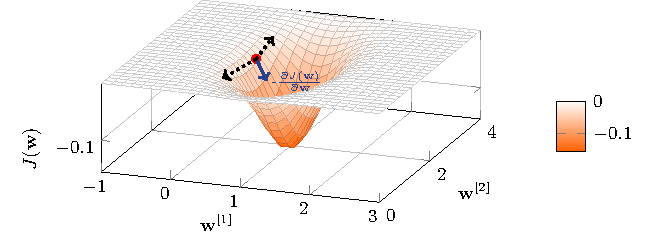
\includegraphics{./Chapter5/Figures/fig-gradient-descent.pdf}
\caption{函数上一个点沿着不同方向移动的示例}
\label{fig:5-43}
\end{figure}
%-------------------------------------------

\parinterval 应用梯度下降算法时,首先需要初始化参数$\mathbf{w}$。一般情况下深度学习中的参数应该初始化为一个不太大的随机数。一旦初始化$\mathbf{w}$后,就开始对模型进行不断的更新,{\small\sffamily\bfseries{参数更新的规则}}\index{参数更新的规则}(Update Rule)\index{Update Rule}为:
\begin{eqnarray}
\mathbf w_{t+1}&=&\mathbf w_{t}-\alpha \cdot \frac{\partial J(\mathbf w)}{\partial \mathbf w}
\label{eq:5-29}
\end{eqnarray}

\noindent 其中$t $表示更新的步数,$ \alpha $是一个超参数,被称作{\small\sffamily\bfseries{学习率}}\index{学习率}(Learning Rate)\index{Learning Rate},表示更新步幅的大小。$ \alpha $的设置需要根据任务进行调整。

\parinterval 从优化的角度看,梯度下降是一种典型的 {\small\bfnew{基于梯度的方法}}\index{基于梯度的方法}(Gradient-based Method)\index{Gradient-based Method},属于基于一阶导数的方法。其他类似的方法还有牛顿法、共轭方向法、拟牛顿法等。在具体实现时,公式\ref{eq:5-29}可以有以下不同的形式。\\

%----------------------------------------------------------------------------------------
%
%----------------------------------------------------------------------------------------

\vspace{0.5em}
\noindent {\small\sffamily\bfseries{批量梯度下降\index{批量梯度下降}(Batch Gradient Descent)\index{Batch Gradient Descent}}}
\vspace{0.5em}

\parinterval 批量梯度下降是梯度下降方法中最原始的形式,这种梯度下降方法在每一次迭代时使用所有的样本进行参数更新。参数优化的目标函数是
\begin{eqnarray}
J(\mathbf w)&=&\frac{1}{n}\sum_{i=1}^{n}{L(\mathbf x_i,\mathbf {\widetilde y}_i;\mathbf w)}
\label{eq:5-30}
\end{eqnarray}

\parinterval 式\ref{eq:5-30}是式\ref{eq:5-29}的严格实现,也就是将全部训练样本的平均损失作为目标函数。由全数据集确定的方向能够更好地代表样本总体,从而朝着模型在数据上整体优化所在的方向更新参数。

\parinterval 不过,这种方法的缺点也十分明显,因为要在全部训练数据上最小化损失,每一次参数更新都需要计算在所有样本上的损失。在使用海量数据进行训练的情况下,这种计算是非常消耗时间的。当训练数据规模很大时,很少使用这种方法。

%----------------------------------------------------------------------------------------
%
%----------------------------------------------------------------------------------------

\vspace{0.5em}
\noindent {\small\sffamily\bfseries{随机梯度下降\index{随机梯度下降}(Stochastic Gradient Descent)\index{Stochastic Gradient Descent}}}
\vspace{0.5em}

\parinterval 随机梯度下降(简称SGD)不同于批量梯度下降,每次迭代只使用一个样本对参数进行更新。SGD的目标函数是
\begin{eqnarray}
J(\mathbf w)&=&L(\mathbf x_i,\mathbf {\widetilde y}_i;\mathbf w)
\label{eq:5-31}
\end{eqnarray}

\noindent 由于每次只随机选取一个样本$(\mathbf x_i,\mathbf {\widetilde y}_i)$进行优化,这样更新的计算代价低,参数更新的速度大大加快,而且也适用于利用少量样本进行在线学习的情况\footnote{比如,训练数据不是一次给定的,而是随着模型的使用不断追加的。这时,需要不断地用新的训练样本更新模型,这种模式也被称作{\scriptsize\bfnew{在线学习}}(Online Learning)。}。

\parinterval 因为随机梯度下降算法每次优化的只是某一个样本上的损失,所以它的问题也非常明显:单个样本上的损失无法代表在全部样本上的损失,因此参数更新的效率低,方法收敛速度极慢。即使在目标函数为强凸函数的情况下,SGD仍旧无法做到线性收敛。

%----------------------------------------------------------------------------------------
%
%----------------------------------------------------------------------------------------

\vspace{0.5em}
\noindent {\small\sffamily\bfseries{小批量梯度下降\index{小批量梯度下降}(Mini-Batch Gradient Descent)\index{Mini-Batch Gradient Descent}}}
\vspace{0.5em}

\parinterval 为了综合批量梯度下降和随机梯度下降的优缺点,在实际应用中一般采用这两个算法的折中\ \dash \ 小批量梯度下降。其思想是:每次迭代计算一小部分训练数据的损失函数,并对参数进行更新。这一小部分数据被称为一个批次(mini-batch或者batch)。小批量梯度下降的参数优化的目标函数如下:
\begin{eqnarray}
J(\mathbf w)&=&\frac{1}{m}\sum_{i=j}^{j+m-1}{L(\mathbf x_i,\mathbf {\widetilde y}_i;\mathbf w)}
\label{eq:5-32}
\end{eqnarray}

\noindent 其中$ m $表示一个批次中的样本的数量,$ j $表示这个批次在全体训练数据的起始位置。这种方法可以更充分的利用GPU设备,因为批次中的样本可以一起计算。而且每次使用多个样本可以大大减小使模型收敛所需要的参数更新次数。但是需要注意的是批次大小的选择对模型的最终性能是存在一定影响的。

%----------------------------------------------------------------------------------------
%    NEW SUBSUB-SECTION
%----------------------------------------------------------------------------------------

\subsubsection{梯度获取}

\parinterval 梯度下降算法的一个核心是要得到目标函数相对于参数的梯度。下面将介绍三种常见的求梯度方法:数值微分、符号微分和自动微分,深度学习实现过程中多是采用自动微分方法计算梯度\cite{baydin2017automatic}。

%----------------------------------------------------------------------------------------
%
%----------------------------------------------------------------------------------------

\vspace{0.5em}
\noindent {\small\sffamily\bfseries{数值微分\index{数值微分}(Numerical Differentiation)\index{Numerical Differentiation}}}
\vspace{0.5em}

\parinterval 数学上,梯度的求解其实就是求函数偏导的问题。导数是用极限来定义的,如下:
\begin{eqnarray}
\frac{\partial L(\mathbf w)}{\partial \mathbf w}&=&\lim\limits_{\Delta \mathbf w \to 0}\frac{L(\mathbf w+\Delta \mathbf w)-L(\mathbf w-\Delta \mathbf w)}{2\Delta \mathbf w}
\label{eq:5-33}
\end{eqnarray}

\noindent 其中,$ \Delta \mathbf w $表示参数的一个很小的变化值。式\ref{eq:5-33}也被称作导数的双边定义。如果一个函数是初等函数,可以用求导法则来求得其导函数。如果不知道函数导数的解析式,则必须利用数值方法来求解该函数在某个点上的导数,这种方法就是数值微分。

\parinterval 数值微分根据导数的原始定义完成,根据公式可知,要得到损失函数在某个参数状态$ \mathbf w $下的梯度,可以将$ \mathbf w $增大或减小一点($ \Delta \mathbf w $),例如,取$ \Delta \mathbf w=0.0001 $,之后观测损失函数的变化与$ \Delta \mathbf w $的比值。$ \Delta \mathbf w $的取值越小计算的结果越接近导数的真实值,但是对计算的精度要求越高。

\parinterval 这种求梯度的方法很简单,但是计算量很大,求解速度非常慢,而且这种方法会造成{\small\sffamily\bfseries{截断误差}}\index{截断误差}(Truncation Error)\index{Truncation Error}和{\small\sffamily\bfseries{舍入误差}}\index{舍入误差}(Round-off Error)\index{Round-off Error}。在网络比较复杂、参数量稍微有点大的模型上一般不会使用这种方法。

\parinterval 截断误差和舍入误差是如何造成的呢?数值微分方法求梯度时,需用极限或无穷过程来求得。然而计算机需要将求解过程化为一系列有限的算术运算和逻辑运算。这样就要对某种无穷过程进行``截断'',即仅保留无穷过程的前段有限序列而舍弃它的后段。这就带来截断误差;舍入误差,是指运算得到的近似值和精确值之间的差异。由于数值微分方法计算复杂函数的梯度问题时,经过无数次的近似,每一次近似都产生了舍入误差,在这样的情况下,误差会随着运算次数增加而积累得很大,最终得出没有意义的运算结果。实际上,截断误差和舍入误差在训练复杂神经网络中,特别是使用低精度计算时,也会出现,因此是实际系统研发中需要注意的问题。

\parinterval 尽管数值微分不适用于大模型中的梯度求解,但是由于其非常简单,因此经常被用于检验其他梯度计算方法的正确性。比如在实现反向传播的时候(详见\ref{sec:5.4.6}节),可以检验求导是否正确(Gradient Check),这个过程就是利用数值微分实现的。\\ \\

%----------------------------------------------------------------------------------------
%
%----------------------------------------------------------------------------------------

\noindent {\small\sffamily\bfseries{ 符号微分\index{符号微分}(Symbolic Differentiation)\index{Symbolic Differentiation}}}
\vspace{0.5em}

\parinterval 顾名思义,符号微分就是通过建立符号表达式求解微分的方法:借助符号表达式和求导公式,推导出目标函数关于自变量的微分表达式,最后再带入具体数值得到微分结果。例如,对于表达式$ L(\mathbf w)=\mathbf x\cdot \mathbf w+2\mathbf w^2 $,可以手动推导出微分表达式$ \frac{\partial L(\mathbf w)}{\partial \mathbf w}=\mathbf x+4\mathbf w  $,最后将具体数值$ \mathbf x = {(\begin{array}{cc} 2 & -3\end{array})} $和$ \mathbf w = {(\begin{array}{cc} -1 & 1\end{array})} $带入后,得到微分结果$\frac{\partial L(\mathbf w)}{\partial \mathbf w}= {(\begin{array}{cc} 2 & -3\end{array})}+4{(\begin{array}{cc} -1 & 1\end{array})}= {(\begin{array}{cc} -2 & 1\end{array})}$。

\parinterval  使用这种求梯度的方法,要求必须将目标函数转化成一种完整的数学表达式,这个过程中存在{\small\bfnew{表达式膨胀}}\index{表达式膨胀}(Expression Swell)\index{Expression Swell}的问题,很容易导致符号微分求解的表达式急速``膨胀'',大大增加系统存储和处理表达式的负担。关于这个问题的一个实例请看表\ref{tab:5-4}。在深层的神经网络中,神经元数量和参数量极大,损失函数的表达式会非常冗长,不易存储和管理,而且,仅仅写出损失函数的微分表达式就是一个很庞大的工作量。从另一方面来说,这里真正需要的是微分的结果值,而不是微分表达式,推导微分表达式仅仅是求解过程中的中间产物。

%--------------------------------------------------------------------
\begin{table}[htp]
\centering
\caption{符号微分的表达式随函数的规模增加而膨胀}
\label{tab:5-4}
\small
\begin{tabular}{l | l l}
\rule{0pt}{18pt}     函数 & 微分表达式 & 化简的微分表达式  \\
\hline
\rule{0pt}{18pt}     $x$ & $1$ & $1$ \\
\rule{0pt}{18pt}     $x\cdot(x+1)$ & $(x+1)+x$ & $2x + 1$ \\
\rule{0pt}{18pt}     $x\cdot(x+1)\cdot$ & $(x+1)\cdot(x^2+x+1)$ & $4x^3+6x^2$ \\
$(x^2+x+1)$ & $+x\cdot(x^2+x+1)$ & $+4x+1$ \\
                     & $+x\cdot(x+1)\cdot(2x+1)$ & \\
\rule{0pt}{18pt}     $(x^2+x)\cdot$ & $(2x+1)\cdot(x^2+x+1)\cdot$ & $8x^7+28x^6$ \\
$(x^2+x+1)\cdot$ & $(x^4+2x^3+2x^2+x+1)$ & $+48x^5+50x^4$ \\
$(x^4+2x^3$ & $+(2x+1)\cdot(x^2+x)\cdot$ & $+36x^3+18x^2$ \\
$+2x^2+x+1)$ & \ \ $(x^4+2x^3+2x^2+x+1)$ & $+6x+1$ \\
 & $+(x^2+x)\cdot(x^2+x+1)\cdot$ & \\
 & \ \ $(4x^3+6x^2+4x+1)$ & \\
\end{tabular}
\end{table}
%--------------------------------------------------------------------

%----------------------------------------------------------------------------------------
%
%----------------------------------------------------------------------------------------

\vspace{0.5em}
\noindent {\small\sffamily\bfseries{自动微分\index{自动微分}(Automatic Differentiation)\index{Automatic Differentiation}}}
\vspace{0.5em}

\parinterval  自动微分是一种介于数值微分和符号微分的方法:将符号微分应用于最基本的算子,如常数、幂函数、指数函数、对数函数、三角函数等,然后代入数值,保留中间结果,最后再应用于整个函数。通过这种方式,将复杂的微分变成了简单的步骤,这些步骤完全自动化,而且容易进行存储和计算。

\parinterval  由于它只对基本函数或常数运用符号微分法则,所以它非常适合嵌入编程语言的循环条件等结构中,形成一种程序化的微分过程。在具体实现时,自动微分往往被当做是一种基于图的计算,相关的理论和技术方法相对成熟,因此是深度学习中使用最广泛的一种方法。不同于一般的编程模式,图计算先生成计算图,然后按照计算图执行计算过程。

\parinterval  自动微分可以用一种{\small\sffamily\bfseries{反向模式}}\index{反向模式}(Backward Mode)\index{Backward Mode}即反向传播思想进行描述。首先,从神经网络的输入,逐层计算每层网络的输出值。如图\ref{fig:5-44},第$ i $层的输出$ \mathbf h_i $作为第$ i+1 $层的输入,数据流在神经网络内部逐层传递。

%----------------------------------------------
\begin{figure}[htp]
\centering
%%%------------------------------------------------------------------------------------------------------------
\begin{tikzpicture}
\begin{scope}
\tikzstyle{layernode} = [draw,thick,fill=ugreen!30!white,blur shadow={shadow xshift=1pt,shadow yshift=-1pt}];

\node [anchor=center,layernode,minimum height=4em,minimum width=1em] (layer01) at (0,0) {};
\node [anchor=north west,layernode,minimum height=3em,minimum width=1em] (layer02) at ([xshift=3em]layer01.north east) {};
\node [anchor=south west,layernode,minimum height=3em,minimum width=1em] (layer03) at ([xshift=7em]layer01.south east) {};
\node [anchor=south west,layernode,minimum height=4em,minimum width=1em] (layer04) at ([xshift=11em]layer01.south east) {};
\node [anchor=south west,layernode,minimum height=4em,minimum width=1em] (layer05) at ([xshift=3em]layer04.south east) {};

\node [anchor=east] (input) at ([xshift=-1em]layer01.west){\scriptsize{输入}};
\node [anchor=west] (output) at ([xshift=1em]layer05.east){\scriptsize{输出}};


{
\draw [->,very thick,ublue] ([xshift=-1em]layer01.west) -- ([xshift=-0.1em]layer01.west)node [pos=0.5,above] {\small{\ding{172}}};;
}
{
\draw [->,very thick,ublue] ([xshift=0.1em,yshift=-0.5em]layer01.north east) -- ([xshift=-0.1em,yshift=-0.5em]layer02.north west)node [pos=0.5,above] {\small{\ding{173}}};
}
{
\draw [->,very thick,ublue] ([xshift=0.1em,yshift=0.5em]layer01.south east) -- ([xshift=-0.1em,yshift=0.5em]layer03.south west)node [pos=0.5,below] {\small{\ding{174}}};
}
{
\draw [->,very thick,ublue] ([xshift=0.1em,yshift=-0.5em]layer02.north east) -- ([xshift=-0.1em,yshift=-0.5em]layer04.north west)node [pos=0.5,above] {\small{\ding{175}}};
\draw [->,very thick,ublue] ([xshift=0.1em,yshift=0.5em]layer03.south east) -- ([xshift=-0.1em,yshift=0.5em]layer04.south west)node [pos=0.5,below] {\small{\ding{176}}};
\draw [->,very thick,ublue] ([xshift=0.1em]layer04.east) -- ([xshift=-0.1em]layer05.west)node [pos=0.5,above] {\small{\ding{177}}};
\draw [->,very thick,ublue] ([xshift=0.1em]layer05.east) -- ([xshift=1.0em]layer05.east)node [pos=0.5,above] {\small{\ding{178}}};
}



{
\draw [<-,thin] ([xshift=0.3em,yshift=0.3em]layer04.east) .. controls +(35:1) and +(215:1) .. ([xshift=-2em,yshift=0.3em]layer05.north west) node [pos=1,above] {\scriptsize{前向:层$i$ 的输出$h_{i}$}};
}


\end{scope}
\end{tikzpicture}
%%%------------------------------------------------------------------------------------------------------------


\caption{前向计算示意图}
\label{fig:5-44}
\end{figure}
%-------------------------------------------

\parinterval  前向计算实际上就是网络构建的过程,所有的计算都会被转化为计算图上的节点,前向计算和反向计算都依赖计算图来完成。构建计算图有以下两种实现方式:

\begin{itemize}
\vspace{0.5em}
\item 动态图(如Pytorch、NiuTensor等):前向计算与计算图的搭建同时进行,函数表达式写完即能得到前向计算的结果,有着灵活、易于调试的优点。
\vspace{0.5em}
\item 静态图(如Tensorflow):先搭建计算图,后执行运算,函数表达式完成后,并不能得到前向计算结果,需要显性调用一个Forward函数。但是计算图可以进行深度优化,执行效率较高。
\vspace{0.5em}
\end{itemize}

\parinterval  对于反向计算的实现,一般从神经网络的输出开始,逆向逐层计算每层网络输入所对应的微分结果。如图\ref{fig:5-45},在第$ i $层计算此处的梯度$ \frac{\partial L}{\partial \mathbf h_i} $,并将微分值向前一层传递,根据链式法则继续计算梯度。

%----------------------------------------------
\begin{figure}[htp]
\centering
%%%------------------------------------------------------------------------------------------------------------
\begin{tikzpicture}
\begin{scope}
\tikzstyle{layernode} = [draw,thick,fill=ugreen!30!white,blur shadow={shadow xshift=1pt,shadow yshift=-1pt}];

\node [anchor=center,layernode,minimum height=4em,minimum width=1em] (layer01) at (0,0) {};
\node [anchor=north west,layernode,minimum height=3em,minimum width=1em] (layer02) at ([xshift=3em]layer01.north east) {};
\node [anchor=south west,layernode,minimum height=3em,minimum width=1em] (layer03) at ([xshift=7em]layer01.south east) {};
\node [anchor=south west,layernode,minimum height=4em,minimum width=1em] (layer04) at ([xshift=11em]layer01.south east) {};
\node [anchor=south west,layernode,minimum height=4em,minimum width=1em] (layer05) at ([xshift=3em]layer04.south east) {};

\node [anchor=east] (input) at ([xshift=-1em]layer01.west){\scriptsize{输入}};
\node [anchor=west] (output) at ([xshift=1em]layer05.east){\scriptsize{输出}};
{
\draw [<-,very thick,red] ([xshift=-1em,yshift=-0.3em]layer01.west) -- ([xshift=-0.1em,yshift=-0.3em]layer01.west)node [pos=0.5,above] {\small{\ding{178}}};
\draw [<-,very thick,red] ([xshift=0.1em,yshift=-0.8em]layer01.north east) -- ([xshift=-0.1em,yshift=-0.8em]layer02.north west)node [pos=0.5,above] {\small{\ding{177}}};
\draw [<-,very thick,red] ([xshift=0.1em,yshift=0.2em]layer01.south east) -- ([xshift=-0.1em,yshift=0.2em]layer03.south west)node [pos=0.5,below] {\small{\ding{176}}};
\draw [<-,very thick,red] ([xshift=0.1em,yshift=-0.8em]layer02.north east) -- ([xshift=-0.1em,yshift=-0.8em]layer04.north west)node [pos=0.5,above] {\small{\ding{175}}};
\draw [<-,very thick,red] ([xshift=0.1em,yshift=0.2em]layer03.south east) -- ([xshift=-0.1em,yshift=0.2em]layer04.south west)node [pos=0.5,below] {\small{\ding{174}}};
\draw [<-,very thick,red] ([xshift=0.1em,yshift=-0.3em]layer04.east) -- ([xshift=-0.1em,yshift=-0.3em]layer05.west)node [pos=0.5,above] {\small{\ding{173}}};
\draw [<-,very thick,red] ([xshift=0.1em,yshift=-0.3em]layer05.east) -- ([xshift=1.0em,yshift=-0.3em]layer05.east)node [pos=0.5,above] {\small{\ding{172}}};
}


{
\draw [<-,thin] ([xshift=0.3em,yshift=-0.7em]layer04.east) .. controls +(-35:1) and +(145:1) .. ([xshift=-2em,yshift=-0.9em]layer05.south west) node [pos=1,below] {\scriptsize{反向:$h_{i}$ 处的梯度$\frac{\partial L}{\partial h_i}$}};
}

\end{scope}
\end{tikzpicture}
%%%------------------------------------------------------------------------------------------------------------


\caption{反向计算示意图}
\label{fig:5-45}
\end{figure}
%-------------------------------------------

\parinterval  反向计算也是深度学习中反向传播方法的基础。其实现的内部细节将在\ref{sec:5.4.6}节详细阐述,所以在这里不再赘述。

%----------------------------------------------------------------------------------------
%    NEW SUBSUB-SECTION
%----------------------------------------------------------------------------------------

\subsubsection{基于梯度的方法的变种和改进}\label{sec:5.4.2.3}

\parinterval  参数优化通常基于梯度下降算法,即在每个更新步骤$ t $,沿梯度方向更新参数:
\begin{eqnarray}
\mathbf w_{t+1}&=&\mathbf w_{t}-\alpha \cdot \frac{\partial J(\mathbf w_t)}{\partial \mathbf w_t}
\label{}
\end{eqnarray}

\noindent 其中$ \alpha $是一个超参数,表示更新步幅的大小,称作{\small\bfnew{学习率}}\index{学习率}(Learning Rate)\index{Learning Rate}。当然,这是一种最基本的梯度下降方法。如果函数的形状非均向,比如呈延伸状,搜索最优点的路径就会非常低效,因为这时梯度的方向并没有指向最小值的方向,并且随着参数的更新,梯度方向往往呈锯齿状,这将是一条相当低效的路径;此外这种梯度下降算法并不是总能到达最优点,而是在其附近徘徊;还有一个最令人苦恼的问题\ \dash \ 设置学习率,如果学习率设置的比较小,会导致训练收敛速度慢,如果学习率设置的比较大,会导致训练过程中因为优化幅度过大而频频跳过最优点。我们希望网络在优化的时候损失函数有一个很好的收敛速度同时又不至于摆动幅度太大。

\parinterval  针对以上问题,很多学者尝试对梯度下降方法做出改进,如Momentum, Adagrad, Adadelta, RMSprop, Adam, AdaMax, Nadam, AMSGrad等等,在这里将介绍Momentum、AdaGrad、RMSprop、Adam这4 种方法。

%----------------------------------------------
\begin{figure}[htp]
\centering

%%%------------------------------------------------------------------------------------------------------------
\begin{tikzpicture}
\begin{scope}


\node [anchor=center,color=red] (node1) at (0,0) {};
\node [anchor=north,color=red] (node4) at ([xshift=9.0em,yshift=0.88em]node1.south) {\large{$\bullet$}};
\node [anchor=north,color=red] (node5) at ([xshift=6.35em,yshift=-2.5em]node1.south) {\large{$\bullet$}};
\node [anchor=north,color=red] (node6) at ([xshift=3.8em,yshift=-0.5em]node1.south) {\large{$\bullet$}};
\node [anchor=north,color=red] (node7) at ([xshift=2.6em,yshift=-2.0em]node1.south) {\large{$\bullet$}};
\node [anchor=north,color=red] (node8) at ([xshift=1.22em,yshift=-0.91em]node1.south) {\large{$\bullet$}};
\node [anchor=north,color=red] (node9) at ([xshift=0.6em,yshift=-1.7em]node1.south) {\large{$\bullet$}};
\node [anchor=north,color=red] (node10) at ([xshift=0.0em,yshift=-1.2em]node1.south) {\large{$\bullet$}};

\draw[-,ublue,line width=0.3mm]([xshift=0.5em,yshift=0.46em]node4.south west)--([xshift=-0.5em,yshift=-0.4em]node5.north east);
\draw[-,ublue,line width=0.3mm]([xshift=-0.45em,yshift=0.52em]node6.south east)--([xshift=0.47em,yshift=-0.43em]node5.north west);
\draw[-,ublue,line width=0.3mm]([xshift=0.5em,yshift=0.46em]node6.south west)--([xshift=-0.5em,yshift=-0.4em]node7.north east);
\draw[-,ublue,line width=0.3mm]([xshift=-0.45em,yshift=0.52em]node8.south east)--([xshift=0.47em,yshift=-0.43em]node7.north west);
\draw[-,ublue]([xshift=0.5em,yshift=0.46em]node8.south west)--([xshift=-0.5em,yshift=-0.4em]node9.north east);
\draw[-,ublue,line width=0.3mm]([xshift=-0.78em,yshift=0.77em]node9.south east)--([xshift=0.78em,yshift=-0.68em]node10.north west);




\draw [-,ublue] (0,0) .. controls (2,0) and (3,-1.0)..(3,-1.5) .. controls (3,-2.2) and (2,-1.75)..(1.5,-1.65)..controls (1.5,-1.65) and (0.5,-1.45)..(0,-1.45)..controls (-0.5,-1.45) and (-1.5,-1.65)..(-1.5,-1.65)..controls (-2,-1.75)and (-3,-2.2).. (-3,-1.5)..controls (-3,-1.0) and (-2,0)..(0,0);

\draw [-,ublue] (0,0.5)..controls (2,0.5) and (4,-1.0).. (4,-1.7)..controls(4,-2.6)and (3,-2.3)..(2,-2.05)..controls (2,-2.05) and (1,-1.80)..(0,-1.80)..controls (-1,-1.80)and (-2,-2.05)..(-2,-2.05)..controls(-3,-2.3)and(-4,-2.6)..(-4,-1.7)..controls(-4,-1.0)and (-2,0.5)..(0,0.5);

\draw[-,ublue](0,1.0)..controls(3,1.0) and (5,-1.0)..(5,-1.9)..controls (5,-3.2)and (4,-2.7)..(3,-2.5)..controls (3,-2.5) and (2,-2.20)..(0,-2.15)..controls (-2,-2.20)and (-3,-2.5)..(-3,-2.5)..controls (-4,-2.7) and (-5,-3.2) ..(-5,-1.9)..controls (-5,-1.0) and (-3,1.0)..(0,1.0);

\draw[-,ublue] (0,-0.3)..controls (1.5,-0.3)and (2.5,-1.0)..(2.5,-1.4)..controls(2.5,-1.8)and (2,-1.55)..(1.5,-1.45) ..controls (1.5,-1.45) and (0.5,-1.25)..(0,-1.25) .. controls(-0.5,-1.25)and (-1.5,-1.45)..(-1.5,-1.45)..controls(-2,-1.55)and (-2.5,-1.8) ..(-2.5,-1.4)..controls(-2.5,-1.0) and (-1.5,-0.3)..(0,-0.3);

\draw[-,ublue](0,-0.5)..controls (1.0,-0.5) and (1.9,-0.8)..(1.9,-1.3)..controls(1.9,-1.5)and (1.5,-1.3)..(1.0,-1.2) ..controls(1.0,-1.2) and (0.5,-1.1)..(0,-1.1)..controls(-0.5,-1.1) and (-1.0,-1.2)..(-1.0,-1.2)..controls (-1.5,-1.3)and (-1.9,-1.5)..(-1.9,-1.3) ..controls(-1.9,-0.8)and (-1.0,-0.5) ..(0,-0.5);

\draw[-,ublue](0,-0.7)..controls(1.0,-0.7) and (1.4,-0.9)..(1.4,-1.1) .. controls(1.4,-1.25) and (1.2,-1.15)..(1.0,-1.1)..controls(1.0,-1.1) and (0.5,-0.95)..(0,-0.95)..controls(-0.5,-0.95)and (-1.0,-1.1) ..(-1.0,-1.1)..controls(-1.2,-1.15) and (-1.4,-1.25)..(-1.4,-1.1)..controls(-1.4,-0.9) and (-1.0,-0.7)..(0,-0.7);

\draw[-,ublue](0,-0.75)..controls(0.7,-0.75)and (1.0,-0.9)..(1.0,-1.0)..controls(1.0,-1.05) and (0.9,-1.05)..(0.7,-1.0)..controls(0.5,-0.95)and (0.3,-0.9)..(0,-0.9)..controls(-0.3,-0.9)and (-0.5,-0.95)..(-0.7,-1.0)..controls(-0.9,-1.05)and (-1.0,-1.05)..(-1.0,-1.0) ..controls(-1.0,-0.9)and (-0.7,-0.75)..(0,-0.75);

\draw[-,ublue](0,-0.8)..controls(0.5,-0.8) and (0.6,-0.85)..(0.6,-0.9)..controls(0.6,-0.93)and (0.5,-0.91)..(0.3,-0.88)..controls(0.2,-0.87)and (0.1,-0.86)..(0,-0.86)..controls(-0.1,-0.86)and(-0.2,-0.87)..(-0.3,-0.88)..controls(-0.5,-0.91) and(-0.6,-0.93) ..(-0.6,-0.9)..controls(-0.6,-0.85)and (-0.5,-0.8)..(0,-0.8);


\node [anchor=north] (labela) at (0,-2.7) {\footnotesize{(a)梯度下降算法中的``锯齿''现象}};

\end{scope}

%%%%%%%%%%%%%%%%%%%%%%%%%%%
\begin{scope}[yshift=-1.8in]


\node [anchor=center,color=red] (node1) at (0,0) {};

\node [anchor=north,color=red] (node2) at ([xshift=0.0em,yshift=-1.2em]node1.south) {\large{$\bullet$}};
\node [anchor=north,color=red] (node3) at ([xshift=3.55em,yshift=-0.981em]node1.south) {\large{$\bullet$}};
\node [anchor=north,color=red] (node4) at ([xshift=7.75em,yshift=-2.91em]node1.south) {\large{$\bullet$}};
\node [anchor=north,color=red] (node5) at ([xshift=11.38em,yshift=-1.11em]node1.south) {\large{$\bullet$}};

\draw[-,ublue,line width=0.3mm]([xshift=0.79em,yshift=-0.59em]node2.north west)--([xshift=-0.75em,yshift=0.6em]node3.south east);
\draw[-,ublue,line width=0.3mm]([xshift=0.79em,yshift=0.66em]node3.south west)--([xshift=-0.76em,yshift=-0.5em]node4.north east);
\draw[-,ublue,line width=0.3mm]([xshift=0.79em,yshift=-0.59em]node4.north west)--([xshift=-0.75em,yshift=0.6em]node5.south east);




\draw [-,ublue] (0,0) .. controls (2,0) and (3,-1.0)..(3,-1.5) .. controls (3,-2.2) and (2,-1.75)..(1.5,-1.65)..controls (1.5,-1.65) and (0.5,-1.45)..(0,-1.45)..controls (-0.5,-1.45) and (-1.5,-1.65)..(-1.5,-1.65)..controls (-2,-1.75)and (-3,-2.2).. (-3,-1.5)..controls (-3,-1.0) and (-2,0)..(0,0);

\draw [-,ublue] (0,0.5)..controls (2,0.5) and (4,-1.0).. (4,-1.7)..controls(4,-2.6)and (3,-2.3)..(2,-2.05)..controls (2,-2.05) and (1,-1.80)..(0,-1.80)..controls (-1,-1.80)and (-2,-2.05)..(-2,-2.05)..controls(-3,-2.3)and(-4,-2.6)..(-4,-1.7)..controls(-4,-1.0)and (-2,0.5)..(0,0.5);

\draw[-,ublue](0,1.0)..controls(3,1.0) and (5,-1.0)..(5,-1.9)..controls (5,-3.2)and (4,-2.7)..(3,-2.5)..controls (3,-2.5) and (2,-2.20)..(0,-2.15)..controls (-2,-2.20)and (-3,-2.5)..(-3,-2.5)..controls (-4,-2.7) and (-5,-3.2) ..(-5,-1.9)..controls (-5,-1.0) and (-3,1.0)..(0,1.0);

\draw[-,ublue] (0,-0.3)..controls (1.5,-0.3)and (2.5,-1.0)..(2.5,-1.4)..controls(2.5,-1.8)and (2,-1.55)..(1.5,-1.45) ..controls (1.5,-1.45) and (0.5,-1.25)..(0,-1.25) .. controls(-0.5,-1.25)and (-1.5,-1.45)..(-1.5,-1.45)..controls(-2,-1.55)and (-2.5,-1.8) ..(-2.5,-1.4)..controls(-2.5,-1.0) and (-1.5,-0.3)..(0,-0.3);

\draw[-,ublue](0,-0.5)..controls (1.0,-0.5) and (1.9,-0.8)..(1.9,-1.3)..controls(1.9,-1.5)and (1.5,-1.3)..(1.0,-1.2) ..controls(1.0,-1.2) and (0.5,-1.1)..(0,-1.1)..controls(-0.5,-1.1) and (-1.0,-1.2)..(-1.0,-1.2)..controls (-1.5,-1.3)and (-1.9,-1.5)..(-1.9,-1.3) ..controls(-1.9,-0.8)and (-1.0,-0.5) ..(0,-0.5);

\draw[-,ublue](0,-0.7)..controls(1.0,-0.7) and (1.4,-0.9)..(1.4,-1.1) .. controls(1.4,-1.25) and (1.2,-1.15)..(1.0,-1.1)..controls(1.0,-1.1) and (0.5,-0.95)..(0,-0.95)..controls(-0.5,-0.95)and (-1.0,-1.1) ..(-1.0,-1.1)..controls(-1.2,-1.15) and (-1.4,-1.25)..(-1.4,-1.1)..controls(-1.4,-0.9) and (-1.0,-0.7)..(0,-0.7);

\draw[-,ublue](0,-0.75)..controls(0.7,-0.75)and (1.0,-0.9)..(1.0,-1.0)..controls(1.0,-1.05) and (0.9,-1.05)..(0.7,-1.0)..controls(0.5,-0.95)and (0.3,-0.9)..(0,-0.9)..controls(-0.3,-0.9)and (-0.5,-0.95)..(-0.7,-1.0)..controls(-0.9,-1.05)and (-1.0,-1.05)..(-1.0,-1.0) ..controls(-1.0,-0.9)and (-0.7,-0.75)..(0,-0.75);

\draw[-,ublue](0,-0.8)..controls(0.5,-0.8) and (0.6,-0.85)..(0.6,-0.9)..controls(0.6,-0.93)and (0.5,-0.91)..(0.3,-0.88)..controls(0.2,-0.87)and (0.1,-0.86)..(0,-0.86)..controls(-0.1,-0.86)and(-0.2,-0.87)..(-0.3,-0.88)..controls(-0.5,-0.91) and(-0.6,-0.93) ..(-0.6,-0.9)..controls(-0.6,-0.85)and (-0.5,-0.8)..(0,-0.8);

\node [anchor=north] (labelb) at (0,-3) {\footnotesize{(b)Momentum梯度下降算法更加``平滑''地更新}};

\end{scope}
\end{tikzpicture}
%%%------------------------------------------------------------------------------------------------------------





\caption{Momentum梯度下降 vs 普通梯度下降}
\label{fig:5-46}
\end{figure}
%-------------------------------------------

%----------------------------------------------------------------------------------------
%
%----------------------------------------------------------------------------------------

\vspace{0.5em}
\noindent {\small\sffamily\bfseries{Momentum \index{Momentum}}}
\vspace{0.5em}

\parinterval  Momentum梯度下降算法的参数更新公式如下\footnote{在梯度下降算法的几种改进方法的公式中,其更新对象是某个具体参数而非参数矩阵,因此不再使用加粗样式}:
\begin{eqnarray}
v_t&=&\beta v_{t-1}+(1-\beta)\frac{\partial L}{\partial w_t}\label{eq:5-34}\\
w_{t+1}&=&w_t-\alpha v_t
\label{eq:5-35}
\end{eqnarray}

\parinterval  该算法引入了一个``动量''的理念\cite{qian1999momentum},它是基于梯度的移动指数加权平均。公式中的$ v_t $是损失函数在前$ t-1 $次更新中累积的梯度动量,$ \beta $是梯度累积的一个指数,这里一般设置值为0.9。所以Momentum梯度下降算法的主要思想就是对网络的参数进行平滑处理,让梯度的摆动幅度变得更小。

\parinterval  这里的``梯度''不再只是现在的损失函数的梯度,而是之前的梯度的加权和。在原始的梯度下降算法中,如果在某个参数状态下,梯度方向变化特别大,甚至与上一次参数更新中梯度方向成90度夹角,下一次参数更新中梯度方向可能又是一次90度的改变,这时参数优化路径将会成``锯齿''状(如图\ref{fig:5-46}所示),优化效率极慢。而Momentum梯度下降算法不会让梯度发生90度的变化,而是让梯度慢慢发生改变:如果当前的梯度方向与之前的梯度方向相同,在原梯度方向上加速更新参数;如果当前的梯度方向与之前的梯度方向相反,并不会产生一个急转弯,而是尽量把优化路径平滑地进行改变。这样做的优点也非常明显,一方面杜绝了``锯齿''状优化路径的出现,另一方面将优化幅度变得更加平滑,不会导致频频跳过最优点。

%----------------------------------------------------------------------------------------
%
%----------------------------------------------------------------------------------------

\vspace{0.5em}
\noindent {\small\sffamily\bfseries{AdaGrad \index{AdaGrad}}}
\vspace{0.5em}

\parinterval  在神经网络的学习中,学习率的设置很重要。学习率过小, 会导致学习花费过多时间;反过来,学习率过大,则会导致学习发散,甚至造成模型的``跑偏''。在深度学习实现过程中,有一种被称为学习率{\small\bfnew{衰减}}\index{衰减}(Decay)\index{Decay}的方法,即最初设置较大的学习率,随着学习的进行,使学习率逐渐减小,这种方法相当于将``全体''参数的学习率值一起降低。AdaGrad梯度下降算法进一步发展了这个思想\cite{duchi2011adaptive}。

\parinterval  AdaGrad会为参数的每个元素适当地调整学习率,与此同时进行学习。其参数更新公式为:
\begin{eqnarray}
z_t&=&z_{t-1}+\frac{\partial L}{\partial w_t} \cdot  \frac{\partial L}{\partial w_t}\label{eq:5-36}\\
w_{t+1}&=&w_t-\eta \frac{1}{\sqrt{z_t}}\cdot \frac{\partial L}{\partial w_t}
\label{eq:5-37}
\end{eqnarray}

\parinterval  这里新出现了变量$ z $,它保存了以前的所有梯度值的平方和,在更新参数时,通过乘以$ \frac{1}{\sqrt{z_t}} $ ,就可以调整学习的尺度。这意味着,变动较大(被大幅度更新)的参数的学习率将变小。也就是说,可以按参数的元素进行学习率衰减,使变动大的参数的学习率逐渐减小。

%----------------------------------------------------------------------------------------
%
%----------------------------------------------------------------------------------------

\vspace{0.5em}
\noindent {\small\sffamily\bfseries{RMSprop \index{RMSprop}}}
\vspace{0.5em}

\parinterval  RMSprop算法是一种自适应学习率的方法\cite{tieleman2012rmsprop},它是对AdaGrad算法的一种改进,可以避免AdaGrad算法中学习率不断单调下降以至于过早衰减的缺点。

\parinterval  RMSProp 算法沿袭了Momentum梯度下降算法中指数加权平均的思路,不过Momentum算法中加权平均的对象是梯度(即$ \frac{\partial L}{\partial w}$),而RMSProp 算法加权平均的对象是梯度的平方(即$ \frac{\partial L}{\partial w} \cdot  \frac{\partial L}{\partial w} $)。RMSProp 算法的参数更新公式为:
\begin{eqnarray}
z_t&=&\gamma z_{t-1}+(1-\gamma) \frac{\partial L}{\partial w_t} \cdot  \frac{\partial L}{\partial w_t}\label{eq:5-38}\\
w_{t+1}&=&w_t-\frac{\eta}{\sqrt{z_t+\epsilon}}\cdot \frac{\partial L}{\partial w_t}
\label{eq:5-39}
\end{eqnarray}

\parinterval  公式中的$ \epsilon $是为了维持数值稳定性而添加的常数,一版可设为 $ 10^{-8} $。和 AdaGrad 的想法类似,模型参数中每个元素都拥有各自的学习率。

\parinterval  RMSProp与AdaGrad相比,学习率的分母部分(即两种梯度下降算法迭代公式中的$ z $)的计算由累积方式变成了指数衰减移动平均。于是,每个参数的学习率并不是呈衰减趋势,而是既可以变小也可以变大,从而避免AdaGrad算法中学习率不断单调下降以至于过早衰减的缺点。

%----------------------------------------------------------------------------------------
%
%----------------------------------------------------------------------------------------

\vspace{0.5em}
\noindent {\small\sffamily\bfseries{Adam \index{Adam} }}
\vspace{0.5em}

\parinterval  Adam梯度下降算法是在RMSProp算法的基础上进行改进的,可以将其看成是带有动量项的RMSProp算法\cite{kingma2014adam}。该算法在自然语言处理领域非常流行。Adam 算法的参数更新公式如下,
\begin{eqnarray}
v_t&=&\beta v_{t-1}+(1-\beta)\frac{\partial L}{\partial w_t}\label{eq:5-40}\\
z_t&=&\gamma z_{t-1}+(1-\gamma) \frac{\partial L}{\partial w_t} \cdot  \frac{\partial L}{\partial w_t}\label{eq:5-41}\\
w_{t+1}&=&w_t-\frac{\eta}{\sqrt{z_t+\epsilon}} v_t
\label{eq:5-42}
\end{eqnarray}

\noindent 可以看到Adam 算法相当于在RMSProp算法中引入了Momentum算法中的动量项,这样做使得Adam算法兼具了Momentum算法和RMSProp算法的优点:既能使梯度更为``平滑''地更新,同时可以为神经网络中的每个参数设置不同的学习率。

\parinterval  需要注意的是包括Adam在内的很多参数更新算法中的学习率都需要人为设置。而且模型学习的效果与学习率的设置关系极大,甚至在研发实际系统时工程师需要进行大量的实验,才能得到最佳的模型。第六章还会具体介绍在机器翻译中参数更新学习率设置的策略。

%----------------------------------------------------------------------------------------
%    NEW SUB-SECTION
%----------------------------------------------------------------------------------------

\subsection{参数更新的并行化策略}

\parinterval  虽然通过GPU可以加速神经网络的运算,但当神经网络较为复杂时,模型训练还是需要几天甚至几周的时间。如果希望尽可能缩短一次学习所需的时间,最直接的想法就是把不同的训练样本分配给多个GPU 或CPU,然后在这些设备上同时进行训练,即实现并行化训练。这种方法也被称作{\small\sffamily\bfseries{数据并行}}\index{数据并行}。具体实现时,有两种常用的并行化策略:(参数)同步更新和(参数)异步更新。

\begin{itemize}
\vspace{0.5em}
\item {\small\sffamily\bfseries{同步更新}}\index{同步更新}(Synchronous Update)\index{Synchronous Update}是指所有计算设备完成计算后,统一汇总并更新参数。当所有设备的反向传播算法完成之后同步更新参数,不会出现单个设备单独对参数进行更新的情况。这种方法效果稳定,但是效率比较低,在同步更新时,每一次参数更新都需要所有设备统一开始、统一结束,如果设备的运行速度不一致,那么每一次参数更新都需要等待最慢的设备结束才能开始。
\vspace{0.5em}
\item {\small\sffamily\bfseries{异步更新}}\index{异步更新}(Asynchronous Update)\index{Asynchronous Update}是指每个计算设备可以随时更新参数。不同设备可以随时读取参数的最新值,然后根据当前参数值和分配的训练样本,各自执行反向传播过程并独立更新参数。由于设备间不需要相互等待,这种方法并行度高。但是不同设备读取参数的时间可能不同,会造成不同设备上的参数不同步,导致这种方法不十分稳定,有可能无法达到较好的训练结果。
\vspace{0.5em}
\end{itemize}

%----------------------------------------------
\begin{figure}[htp]
\centering
%%%------------------------------------------------------------------------------------------------------------
\begin{tikzpicture}

%%%%%%%%%%%%%%%%
% parameter server + processor
\begin{scope}[]

{\scriptsize

\tikzstyle{parametershard} = [draw,thick,minimum width=4em,align=left,rounded corners=2pt]

{
\node[parametershard,anchor=west,fill=yellow!10] (param1) at (0,0) {$W_o$};
\node (param2) at ([xshift=1em]param1.east) {};
\node[parametershard,anchor=west,fill=red!10] (param3) at ([xshift=1em]param2.east) {$W_h$};
\node[anchor=south,inner sep=1pt] (serverlabel) at ([yshift=0.2em]param2.north) {\footnotesize{\textbf{parameter server}: $\mathbf w_{new} = \mathbf w - \alpha\cdot \frac{\partial L}{\partial \mathbf w}$}};
}

\begin{pgfonlayer}{background}
{
\node[rectangle,draw,thick,inner sep=2pt,fill=gray!20] [fit = (param1) (param2) (param3) (serverlabel)] (serverbox) {};
}
\end{pgfonlayer}

\tikzstyle{processor} = [draw,thick,fill=orange!20,minimum width=4em,align=left,rounded corners=2pt]

{
\node [processor,anchor=north,align=center] (processor2) at ([yshift=-1.2in]serverlabel.south) {\scriptsize{Processor 2}\\\scriptsize{on GPU2 (G2)}};
\node [anchor=north] (labela) at ([xshift=4em,yshift=-1em]processor2.south) {\footnotesize {(a)同步更新}};
\node [processor,anchor=east,align=center] (processor1) at ([xshift=-1em]processor2.west) {\scriptsize{Processor 1}\\\scriptsize{on GPU1 (G1)}};
\node [processor,anchor=west,align=center] (processor3) at ([xshift=1em]processor2.east) {\scriptsize{Processor 3}\\\scriptsize{on GPU3 (G3)}};
}

{
\draw[->,very thick,red] ([xshift=-0.5em,yshift=2pt]processor2.north) -- ([xshift=-0.5em,yshift=-2pt]serverbox.south) node [pos=0.5,align=right,xshift=-2em] (pushlabel) {\scriptsize{$\frac{\partial L}{\partial \mathbf w}$}};;
\draw[<-,very thick,blue] ([xshift=0.5em,yshift=2pt]processor2.north) -- ([xshift=0.5em,yshift=-2pt]serverbox.south) node [pos=0.5,align=left,xshift=2.2em] (fetchlabel) {\scriptsize{$\mathbf w_{new}$}};;;
\draw[->,very thick,red] ([xshift=-0.5em,yshift=2pt]processor3.north) --
 ([xshift=3em,yshift=-2pt]serverbox.south);
\draw[<-,very thick,blue] ([xshift=0.5em,yshift=2pt]processor3.north) -- ([xshift=4em,yshift=-2pt]serverbox.south) node [pos=0.5,align=left,xshift=2.2em] (fetchlabel) {\scriptsize{fetch (F)}};
\draw[->,very thick,red] ([xshift=-0.5em,yshift=2pt]processor1.north) -- ([xshift=-4em,yshift=-2pt]serverbox.south) node [pos=0.5,align=right,xshift=-2em] (pushlabel) {\scriptsize{push (P)}};
\draw[<-,very thick,blue] ([xshift=0.5em,yshift=2pt]processor1.north) -- ([xshift=-3em,yshift=-2pt]serverbox.south);
}

%%%%%%%%%%%
% synchronous mode
\tikzstyle{job} = [draw,rotate=90,minimum height=0.25in]

\scriptsize{
{
\node[job,anchor=south west,fill=blue!50] (fetch11) at ([xshift=6em,yshift=1em]processor3.east) {\textbf{F}};
\node[job,anchor=west,fill=orange!30] (minibatch11) at ([yshift=1pt]fetch11.east) {\tiny{minibatch3}};
\node[job,anchor=west,fill=red!50] (push11) at ([yshift=1pt]minibatch11.east) {\textbf{P}};
\node[job,anchor=north west,fill=blue!50] (fetch12) at ([xshift=0.8em]fetch11.south west) {\textbf{F}};
\node[job,anchor=west,fill=orange!30] (minibatch12) at ([yshift=1pt]fetch12.east) {\tiny{minibatch2}};
\node[job,anchor=west,fill=red!50] (push12) at ([yshift=1pt]minibatch12.east) {\textbf{P}};
\node[job,anchor=north west,fill=blue!50] (fetch13) at ([xshift=0.8em]fetch12.south west) {\textbf{F}};
\node[job,anchor=west,fill=orange!30,minimum width=8em] (minibatch13) at ([yshift=1pt]fetch13.east) {\scriptsize{minibatch1}};
\node[job,anchor=west,fill=red!50] (push13) at ([yshift=1pt]minibatch13.east) {\textbf{P}};
\node[anchor=south west,draw,fill=gray!20,minimum width=8.0em] (update11) at ([yshift=4.0em]push11.north east) {Update};

\node[anchor=north] (G11) at (fetch11.west) {\small{G3}};
\node[anchor=north] (G12) at (fetch12.west) {\small{G2}};
\node[anchor=north] (G13) at (fetch13.west) {\small{G1}};
\node[anchor=north,align=center] (synlabel) at (G12.south) {\small{\textbf{Synchronous}}\\\small{\textbf{Training}}};
\draw[->,thick] ([xshift=1em]G13.east) -- ([xshift=1em,yshift=1.4in]G13.east) node [pos=0.5,rotate=90,yshift=-1em] {\small{time line}};
}
}

{
\draw [<->,thin,dotted] ([xshift=-1pt]minibatch11.north) .. controls +(west:3em) and +(east:3em) .. ([xshift=1pt]processor3.east);
\draw [<->,thin,dotted] ([xshift=-1pt]fetch11.north) .. controls +(west:4em) and +(east:4em) .. ([xshift=-0.5em,yshift=0.3in]processor3.north);
\draw [<->,thin,dotted] ([xshift=-1pt]push11.north) -- ([xshift=-4em,yshift=0.8in]processor3.north);
}

{
\draw [<->,thin,dotted] ([xshift=-1pt]update11.west) -- ([xshift=1pt,yshift=-1.5em]serverbox.north east);
}


}

\end{scope}

\begin{scope}[yshift=-2.5in]

{\scriptsize

\tikzstyle{parametershard} = [draw,thick,minimum width=4em,align=left,rounded corners=2pt]

{
\node[parametershard,anchor=west,fill=yellow!10] (param1) at (0,0) {$W_o$};
\node (param2) at ([xshift=1em]param1.east) {};
\node[parametershard,anchor=west,fill=red!10] (param3) at ([xshift=1em]param2.east) {$W_h$};
\node[anchor=south,inner sep=1pt] (serverlabel) at ([yshift=0.2em]param2.north) {\footnotesize{\textbf{parameter server}: $\mathbf w_{new} = \mathbf w - \alpha\cdot \frac{\partial L}{\partial \mathbf w}$}};
}

\begin{pgfonlayer}{background}
{
\node[rectangle,draw,thick,inner sep=2pt,fill=gray!20] [fit = (param1) (param2) (param3) (serverlabel)] (serverbox) {};
}
\end{pgfonlayer}

\tikzstyle{processor} = [draw,thick,fill=orange!20,minimum width=4em,align=left,rounded corners=2pt]

{
\node [processor,anchor=north,align=center] (processor2) at ([yshift=-1.2in]serverlabel.south) {\scriptsize{Processor 2}\\\scriptsize{on GPU2 (G2)}};
\node [anchor=north] (label) at ([xshift=4em,yshift=-1em]processor2.south) {\footnotesize {(b)异步更新}};
\node [processor,anchor=east,align=center] (processor1) at ([xshift=-1em]processor2.west) {\scriptsize{Processor 1}\\\scriptsize{on GPU1 (G1)}};
\node [processor,anchor=west,align=center] (processor3) at ([xshift=1em]processor2.east) {\scriptsize{Processor 3}\\\scriptsize{on GPU3 (G3)}};
}

{
\draw[->,very thick,red] ([xshift=-0.5em,yshift=2pt]processor2.north) -- ([xshift=-0.5em,yshift=-2pt]serverbox.south) node [pos=0.5,align=right,xshift=-2em] (pushlabel) {\scriptsize{$\frac{\partial L}{\partial \mathbf w}$}};;
\draw[<-,very thick,blue] ([xshift=0.5em,yshift=2pt]processor2.north) -- ([xshift=0.5em,yshift=-2pt]serverbox.south) node [pos=0.5,align=left,xshift=2.2em] (fetchlabel) {\scriptsize{$\mathbf w_{new}$}};;;
\draw[->,very thick,red] ([xshift=-0.5em,yshift=2pt]processor3.north) --
 ([xshift=3em,yshift=-2pt]serverbox.south);
\draw[<-,very thick,blue] ([xshift=0.5em,yshift=2pt]processor3.north) -- ([xshift=4em,yshift=-2pt]serverbox.south) node [pos=0.5,align=left,xshift=2.2em] (fetchlabel) {\scriptsize{fetch (F)}};
\draw[->,very thick,red] ([xshift=-0.5em,yshift=2pt]processor1.north) -- ([xshift=-4em,yshift=-2pt]serverbox.south) node [pos=0.5,align=right,xshift=-2em] (pushlabel) {\scriptsize{push (P)}};
\draw[<-,very thick,blue] ([xshift=0.5em,yshift=2pt]processor1.north) -- ([xshift=-3em,yshift=-2pt]serverbox.south);
}

%%%%%%%%%%%
% synchronous mode
\tikzstyle{job} = [draw,rotate=90,minimum height=0.25in]

\scriptsize{
{
\node[job,anchor=south west,fill=blue!50] (fetch21) at ([xshift=6em,yshift=1em]processor3.east) {\textbf{F}};
\node[job,anchor=west,fill=orange!30] (minibatch21) at ([yshift=1pt]fetch21.east) {\tiny{minibatch3}};
\node[job,anchor=west,fill=red!50] (push21) at ([yshift=1pt]minibatch21.east) {\textbf{P}};
\node[job,anchor=north west,fill=blue!50] (fetch22) at ([xshift=0.8em]fetch21.south west) {\textbf{F}};
\node[job,anchor=west,fill=orange!30] (minibatch22) at ([yshift=1pt]fetch22.east) {\tiny{minibatch2}};
\node[job,anchor=west,fill=red!50] (push22) at ([yshift=1pt]minibatch22.east) {\textbf{P}};
\node[job,anchor=north west,fill=blue!50] (fetch23) at ([xshift=0.8em]fetch22.south west) {\textbf{F}};
\node[job,anchor=west,fill=orange!30,minimum width=8em] (minibatch23) at ([yshift=1pt]fetch23.east) {\scriptsize{minibatch1}};
\node[job,anchor=west,fill=red!50] (push23) at ([yshift=1pt]minibatch23.east) {\textbf{P}};
\node[anchor=south west,draw,fill=gray!20,minimum width=0.59in] (update21) at ([yshift=2pt]push21.north east) {Update};
\node[anchor=south west,draw,fill=gray!20,minimum width=0.25in] (update22) at ([yshift=2pt]push23.north east) {\tiny{Upd.}};

\node[anchor=north] (G21) at (fetch21.west) {\small{G3}};
\node[anchor=north] (G22) at (fetch22.west) {\small{G2}};
\node[anchor=north] (G23) at (fetch23.west) {\small{G1}};
\node[anchor=north,align=center] (synlabel) at (G22.south) {\small{\textbf{Asynchronous}}\\\small{\textbf{Training}}};
\draw[->,thick] ([xshift=1em]G23.east) -- ([xshift=1em,yshift=1.4in]G23.east) node [pos=0.5,rotate=90,yshift=-1em] {\small{time line}};

\draw [<->,thin,dotted] ([xshift=-1pt]update21.west) -- ([xshift=1pt,yshift=-1.5em]serverbox.north east);
\draw [<->,thin,dotted] ([xshift=-1pt]update22.west) -- ([xshift=1pt,yshift=-1.5em]serverbox.north east);
}
}

}

\end{scope}

\end{tikzpicture}
%%%------------------------------------------------------------------------------------------------------------





\caption{同步更新与异步更新对比}
\label{fig:5-47}
\end {figure}
%-------------------------------------------

\parinterval  图\ref{fig:5-47}对比了同步更新和异步更新的区别,在这个例子中,使用4台设备对一个两层神经网络中的参数进行更新,其中使用了一个{\small\bfnew{参数服务器}}\index{参数服务器}(Parameter Server\index{Parameter Server})来保存最新的参数,不同设备(Worker,图中的G1、G2、G3)可以通过同步或者异步的方式访问参数服务器。图中的$ \mathbf w_o $和$ \mathbf w_h $分别代表输出层和隐藏层的全部参数,操作push(P) 表示设备向参数服务器传送梯度,操作fetch(F)表示参数服务器向设备传送更新后的参数。

\parinterval  此外,在使用多个设备进行并行训练的时候,由于设备间带宽的限制,大量的数据传输会有较高的延时。对于复杂神经网络来说,设备间参数和梯度传递的时间消耗也会成为一个不得不考虑的因素。有时候,设备间数据传输的时间甚至比模型计算的时间都长,大大降低了并行度\cite{xiao2017fast}。对于这种问题,可以考虑对数据进行压缩或者减少传输的次数来缓解问题。

%----------------------------------------------------------------------------------------
%    NEW SUB-SECTION
%----------------------------------------------------------------------------------------

\subsection{梯度消失、梯度爆炸和稳定性训练}\label{sec:5.4.4}

\parinterval  深度学习中随着神经网络层数的增加,导数可能会出现指数级的下降或者指数级的增加,这种现象分别称为{\small\sffamily\bfseries{梯度消失}}\index{梯度消失}(Gradient Vanishing)\index{Gradient Vanishing}和{\small\sffamily\bfseries{梯度爆炸}}\index{梯度爆炸}(Gradient Explosion)\index{Gradient Explosion}。出现这两种现象的本质原因是反向传播过程中链式法则导致梯度矩阵的多次相乘。这类问题很容易导致训练的不稳定。

%----------------------------------------------------------------------------------------
%    NEW SUBSUB-SECTION
%----------------------------------------------------------------------------------------

\subsubsection{易于优化的激活函数}

\parinterval  网络训练过程中,如果每层网络的梯度都小于1,各层梯度的偏导数会与后面层传递而来的梯度相乘得到本层的梯度,并向前一层传递。该过程循环进行,最后导致梯度指数级地减小,这就产生了梯度消失现象。这种情况会导致神经网络层数较浅的部分梯度接近0。一般来说,产生很小梯度的原因是使用了类似于Sigmoid这样的激活函数,当输入的值过大或者过小的时候这类函数曲线会趋于直线,梯度近似为零。针对这个问题,主要的解决办法是使用更加易于优化的激活函数,比如,使用ReLU代替Sigmoid和Tanh作为激活函数。

\parinterval  缓解梯度消失问题最直接的想法就是希望各层的偏导数大于或等于1。图\ref{fig:5-48}展示了Sigmoid激活函数$ y=\frac{1}{1+e^{-x}}$的函数曲线和导函数曲线,如果使用Sigmoid作为损失函数,其梯度不可能超过0.25,这样经过链式求导之后,很容易发生梯度消失。

%----------------------------------------------
\begin{figure}[htp]
\centering
%%%------------------------------------------------------------------------------------------------------------
\begin{tikzpicture}
\begin{axis}[  
  name=sigmoid,
  width=6cm, height=4.5cm, 
  xtick={-5,-2.5,...,6},
  ytick={0,0.5,1.0},
  xlabel={$x$},
  ylabel={$y$},
  xlabel style={xshift=2.4cm,yshift=0.7cm},
  axis y line=middle,%y轴居中
  ylabel style={xshift=0.1cm,yshift=0cm},
  x axis line style={->},%x轴箭头
  axis line style={very thick},
  axis x line*=bottom,%将上面的x轴去掉,仅保留下面的x轴
  xmin=-6,
  xmax=6,
  ymin=0,
  ymax=1.4]
\addplot[draw=red,very thick]{1/(1 + exp( -x))};
\end{axis}
\node [anchor=north] (labelc) at (2.3,-0.5) {\footnotesize{(a)}};
\begin{axis}[
  at={(sigmoid.east)},
  anchor=east, 
  xshift=6cm,
  yshift=0cm,  
  width=6cm, height=4.5cm, 
  xtick={-4,-2,...,4},
  ytick={0,0.1,0.2},
  xlabel={$x$},
  ylabel={$y$},
  xlabel style={xshift=2.4cm,yshift=0.7cm},
  axis y line=middle,%y轴居中
  ylabel style={xshift=0.1cm,yshift=0cm},
  x axis line style={->},%x轴箭头
  axis line style={very thick},
  axis x line*=bottom,%将上面的x轴去掉,仅保留下面的x轴
  xmin=-6,
  xmax=6,
  ymin=0,
  ymax=0.3]
\addplot[draw=ublue,very thick]{(1/(1 + exp( -x)))*(1-(1/(1 + exp( -x))))};
\end{axis}
\node [anchor=north] (labelc) at (8.2,-0.5) {\footnotesize{(b)}};
\end{tikzpicture}
%%%------------------------------------------------------------------------------------------------------------


\caption{Sigmoid激活函数的函数曲线和导函数曲线}
\label{fig:5-48}
\end {figure}
%-------------------------------------------

\parinterval  同理,Tanh作为激活函数也容易出现梯度消失现象,图\ref{fig:5-49}展示了Tanh激活函数$ y=\frac{e^x-e^{-x}}{e^x+e^{-x}}$的函数曲线和导函数曲线,可以看出,Tanh激活函数比Sigmoid激活函数要好一些,但是Tanh激活函数的导数也小于1,因此无法避免梯度消失现象。

%----------------------------------------------
\begin{figure}[htp]
\centering
%%%------------------------------------------------------------------------------------------------------------
\begin{tikzpicture}
\begin{axis}[  
  name=tanh,
  width=6cm, height=4.5cm, 
  xtick={-5,-2.5,...,6},
  ytick={-1.0,-0.5,0,0.5,1.0},
  xlabel={$x$},
  ylabel={$y$},
  xlabel style={xshift=2.4cm,yshift=2.5cm},
  axis y line=middle,%y轴居中
  ylabel style={xshift=0.1cm,yshift=0cm},
  x axis line style={->},%x轴箭头
  axis line style={very thick},
  axis x line*=middle,%将上面的x轴去掉,仅保留下面的x轴
  xmin=-6,
  xmax=6,
  ymin=-1.2,
  ymax=1.2]
\addplot[draw=red,very thick]{tanh(x)};
\end{axis}
\node [anchor=north] (labelc) at (2.3,-0.5) {\footnotesize{(a)}};
\begin{axis}[  
  at={(tanh.east)},
  anchor=east, 
  xshift=6cm,
  yshift=0cm, 
  width=6cm, height=4.5cm, 
  xtick={-10,-5,...,10},
  ytick={0,0.5,1},
  xlabel={$x$},
  ylabel={$y$},
  xlabel style={xshift=2.4cm,yshift=0.7cm},
  axis y line=middle,%y轴居中
  ylabel style={xshift=0.1cm,yshift=0cm},
  x axis line style={->},%x轴箭头
  axis line style={very thick},
  axis x line*=bottom,%将上面的x轴去掉,仅保留下面的x轴
  xmin=-10,
  xmax=10,
  ymin=0,
  ymax=1.2]
\addplot[draw=ublue,very thick]{1-tanh(x)*tanh(x)};
\end{axis}
\node [anchor=north] (labelc) at (8.2,-0.5) {\footnotesize{(b)}};
\end{tikzpicture}
%%%------------------------------------------------------------------------------------------------------------


\caption{Tanh激活函数的函数曲线和导函数曲线}
\label{fig:5-49}
\end {figure}
%-------------------------------------------

\parinterval  ReLU激活函数的思想也很简单,如果激活函数的导数为1,那么就不存在梯度消失爆炸的问题了。图\ref{fig:5-50}展示了ReLU激活函数$ y={\rm{max}}(0,x)$的函数曲线和导函数曲线。可以很容易看出,ReLU函数的导数在正数部分是恒等于1的,因此在深层网络中使用ReLU激活函数就不会产生很小的梯度。

%----------------------------------------------
\begin{figure}[htp]
\centering
%%%------------------------------------------------------------------------------------------------------------
\begin{tikzpicture}
\begin{axis}[  
  name=relu,
  width=6cm, height=4.5cm, 
  xtick={-1.0,-0.5,...,1.0},
  ytick={0.5,1.0},
  xlabel={$x$},
  ylabel={$y$},
  xlabel style={xshift=2.4cm,yshift=0.7cm},
  axis y line=middle,%y轴居中
  ylabel style={xshift=0.1cm,yshift=0cm},
  x axis line style={->},%x轴箭头
  axis line style={very thick},
  axis x line*=middle,%将上面的x轴去掉,仅保留下面的x轴
  xmin=-1.2,
  xmax=1.2,
  ymin=0,
  ymax=1.2]
\addplot[domain=-1:0,draw=red,very thick]{0};
\addplot[domain=0:1,draw=red,very thick]{x};
\end{axis}
\node [anchor=north] (labelc) at (2.3,-0.5) {\footnotesize{(a)}};
\begin{axis}[  
  at={(relu.east)},
  anchor=east, 
  xshift=6cm,
  yshift=0cm, 
  width=6cm, height=4.5cm, 
  xtick={-4,-2,...,4},
  ytick={0,0.2,...,1.0},
  xlabel={$x$},
  ylabel={$y$},
  xlabel style={xshift=2.4cm,yshift=0.7cm},
  axis y line=middle,%y轴居中
  ylabel style={xshift=0.1cm,yshift=0cm},
  x axis line style={->},%x轴箭头
  axis line style={very thick},
  axis x line*=middle,%将上面的x轴去掉,仅保留下面的x轴
  xmin=-5,
  xmax=5,
  ymin=0,
  ymax=1.2]
\addplot[domain=-4:0,draw=ublue,very thick]{0};
\addplot[domain=0:4,draw=ublue,very thick]{1};
\end{axis}
\node [anchor=north] (labelc) at (8.2,-0.5) {\footnotesize{(b)}};
\end{tikzpicture}
%%%------------------------------------------------------------------------------------------------------------


\caption{ReLU激活函数的函数曲线和导函数曲线}
\label{fig:5-50}
\end {figure}
%-------------------------------------------

\parinterval  当然,梯度消失并不是仅仅可以通过改变激活函数就可以完全消除掉。随着网络层数的增加,很多因素都可能会造成梯度消失。后面也会进一步介绍其他手段,可以综合运用这些方法达到很好的缓解梯度消失问题的目的。

%----------------------------------------------------------------------------------------
%    NEW SUBSUB-SECTION
%----------------------------------------------------------------------------------------

\subsubsection{梯度裁剪}

\parinterval  网络训练过程中,如果参数的初始值过大,而且每层网络的梯度都大于1,反向传播过程中,各层梯度的偏导数都会比较大,会导致梯度指数级地增长直至超出浮点数表示的范围,这就产生了梯度爆炸现象。如果发生这种情况,模型中离输入近的部分比离输入远的部分参数更新得更快,使网络变得非常不稳定。在极端情况下,模型的参数值变得非常大,甚至于溢出。针对梯度爆炸的问题,常用的解决办法为{\small\sffamily\bfseries{梯度裁剪}}\index{梯度裁剪}(Gradient Clipping)\index{Gradient Clipping}。

\parinterval    梯度裁剪的思想是设置一个梯度剪切阈值。在更新梯度的时候,如果梯度超过这个阈值,就将其强制限制在这个范围之内。假设梯度为$ \mathbf g $,梯度剪切阈值为$ \theta $,梯\\ \\度裁剪的公式为
\begin{eqnarray}
\mathbf g&=&{\rm{min}}(\frac{\theta}{\Vert \mathbf g\Vert},1)\mathbf g
\label{eq:5-43}
\end{eqnarray}

\noindent 其中,$ \Vert \cdot \Vert $表示$ l_2 $范数。梯度裁剪经常被使用在层数较多的模型中,如循环神经网络。

%----------------------------------------------------------------------------------------
%    NEW SUBSUB-SECTION
%----------------------------------------------------------------------------------------

\subsubsection{稳定性训练}

\parinterval  为了使神经网络模型训练更加稳定,通常还会考虑其他策略。

\parinterval  (1){\small\bfnew{批量归一化}}\index{批量归一化}(Batch Normalization)\index{Batch Normalization}

\parinterval  批量归一化,顾名思义,是以进行学习时的小批量样本为单位进行归一化\cite{ioffe2015batch}。具体而言,就是对神经网络隐层输出的每一个维度,沿着批次的方向进行均值为0、方差为1的归一化。在深层神经网络中,每一层网络都可以使用批量归一化操作。这样使神经网络任意一层的输入不至于过大或过小,从而防止隐层中异常值导致模型状态的巨大改变。

\parinterval  (2){\small\bfnew{层归一化}}\index{层归一化}(Layer Normalization)\index{Layer Normalization}

\parinterval  类似的,层归一化更多是针对自然语言处理这种序列处理任务\cite{Ba2016LayerN},它和批量归一化的原理是一样的,只是归一化操作是在序列上同一层网络的输出结果上进行的,也就是归一化操作沿着序列方向进行。这种方法可以很好的避免序列上不同位置神经网络输出结果的不可比性。同时由于归一化后所有的结果都转化到一个可比的范围,使得隐层状态可以在不同层之间进行自由组合。

\parinterval  (3){\small\bfnew{残差网络}}\index{残差网络}(Residual Networks)\index{Residual Networks}

\parinterval  最初,残差网络是为了解决神经网络持续加深时的模型退化问题\cite{DBLP:journals/corr/HeZRS15},但是残差结构对解决梯度消失和梯度爆炸问题也有所帮助。有了残差结构,可以很轻松的构建几十甚至上百层的神经网络,而不用担心层数过深造成的梯度消失问题。残差网络的结构如图\ref{fig:5-51}所示:

%----------------------------------------------
\begin{figure}[htp]
\centering
%%%------------------------------------------------------------------------------------------------------------
\begin{tikzpicture}
\begin{scope}


\node [anchor=center] (node6) at (0,0) {};
\node[anchor=west](node6-1) at ([xshift=-0.2em,yshift=-0.6em]node6.east) {\footnotesize{$\rm{ReLU}$}};
\node [anchor=north](node3)at ([yshift=-1.2em]node6.south){$\bigoplus$};
\draw[->,thick]([yshift=-0.32em]node3.north)--(node6.south);

\node [anchor=north,draw,thick](node2)at ([yshift=-1.2em]node3.south){\small{weight layer}};
\draw[->,thick](node2.north)--([yshift=0.35em]node3.south);
\node[anchor=west](node2-1) at ([xshift=2.1em,yshift=1.2em]node2.east) {$\mathbf{x}$};
\node[anchor=north](node2-2) at ([xshift=0.2em,yshift=-0.3em]node2-1.south) {\footnotesize{$\rm{identity}$}};

\node [anchor=east](node4) at ([xshift=-0.2em]node2.west) {$\textrm{F}(\mathbf{x})$};
\node [anchor=east](node5) at ([xshift=-0.3em]node3.west) {$\textrm{F}(\mathbf{x})+\mathbf{x}$};

\node [anchor=north](node1) at ([yshift=-1.8em]node2.south) {};
\draw[->,thick]([yshift=0.0em]node1.north)--(node2.south);
\node [anchor=east](node1-1) at ([xshift=1em,yshift=0.4em]node1.east) {$\mathbf{x}$};
\draw[->,thick]([xshift=-1.3em,yshift=0.8em]node1-1.east)--([xshift=2.7em,yshift=0.8em]node1-1.east)--([xshift=2.7em,yshift=5.35em]node1-1.east)--([xshift=-0.4em]node3.east);




\end{scope}
\end{tikzpicture}
%%%------------------------------------------------------------------------------------------------------------







\caption{残差网络的结构}
\label{fig:5-51}
\end{figure}
%-------------------------------------------

\parinterval  图\ref{fig:5-51}中右侧的曲线叫做{\small\bfnew{跳接}}\index{跳接}(Shortcut Connection)\index{Shortcut Connection},通过跳接在激活函数前,将上一层(或几层)之前的输出与本层计算的输出相加,将求和的结果输入到激活函数中作为本层的输出。假设残差结构的输入为$ \mathbf x_l $,输出为$ \mathbf x_{l+1} $,则有
\begin{eqnarray}
\mathbf x_{l+1}&=&F(\mathbf x_l)+\mathbf x_l
\label{eq:5-44}
\end{eqnarray}

\parinterval  相比较于简单的多层堆叠的结构,残差网络提供了跨层连接结构。这种结构在反向传播中有很大的好处,比如,对于$ \mathbf x_l $处的梯度可以进行如下计算:
\begin{eqnarray}
\frac{\partial L}{\partial \mathbf x_l}&=&\frac{\partial L}{\partial \mathbf x_{l+1}} \cdot  \frac{\partial \mathbf x_{l+1}}{\partial \mathbf x_l}\nonumber\\
&=&\frac{\partial L}{\partial \mathbf x_{l+1}} \cdot \left(1+\frac{\partial F(\mathbf x_l)}{\partial \mathbf x_l}\right)\nonumber\\
&=&\frac{\partial L}{\partial \mathbf x_{l+1}}+\frac{\partial L}{\partial \mathbf x_{l+1}} \cdot  \frac{\partial F(\mathbf x_l)}{\partial \mathbf x_l}
\label{eq:5-45}
\end{eqnarray}

\parinterval  由上式可知,残差网络可以将后一层的梯度$ \frac{\partial L}{\partial \mathbf x_{l+1}} $不经过任何乘法项直接传递到$ \frac{\partial L}{\partial \mathbf x_l} $,从而缓解了梯度经过每一层后多次累乘造成的梯度消失问题。在第六章中还会看到,在机器翻译中残差结构可以和层归一化一起使用,而且这种组合可以取得很好的效果。

%----------------------------------------------------------------------------------------
%    NEW SUB-SECTION
%----------------------------------------------------------------------------------------

\subsection{过拟合}\label{sec:5.4.5}

\parinterval  理想中,我们总是希望尽可能地拟合输入和输出之间的函数关系,即让模型尽量模拟训练数据的中由输入预测答案的行为。然而,在实际应用中,模型在训练数据上的表现不一定代表了其在未见数据上的表现。如果模型训练过程中过度拟合训练数据,最终可能无法对未见数据做出准确的判断,这种现象叫做{\small\sffamily\bfseries{过拟合}}\index{过拟合}(Overfitting)\index{Overfitting}。随着模型复杂度增加,特别在神经网络变得更深、更宽时,过拟合问题会表现得更为突出。如果训练数据量较小,而模型又很复杂,可以``完美''地拟合这些数据,这时过拟合也很容易发生。所以在模型训练时,往往不希望去完美拟合训练数据中的每一个样本。

\parinterval  {\small\sffamily\bfseries{正则化}}\index{正则化}(Regularization)\index{Regularization}是常见的缓解过拟合问题的手段,通过在损失函数中加上用来刻画模型复杂程度的正则项来惩罚过度复杂的模型,从而避免神经网络过度学习造成过拟合。引入正则化处理之后目标函数变为$ J(\mathbf w)+\lambda R(\mathbf w) $,其中$ J(\mathbf w) $是原来的代价函数,$ R(\mathbf w) $即为正则项,$ \lambda $用来调节正则项对结果影响的程度。

\parinterval  过拟合的模型通常会表现为部分非零参数过多或者参数的值过大。这种参数产生的原因在于模型需要复杂的参数才能匹配样本中的个别现象甚至噪声。基于此,常见的正则化方法有L1正则化和L2正则化,其命名方式是由$ R(\mathbf w) $的计算形式来决定的。在L1正则化中,$ R(\mathbf w) $即为参数$ w $的$ l_1 $范数,即$ R(\mathbf w) ={\Vert \mathbf w\Vert}_1=\sum_{i=1}^{n}{\vert w_i\vert} $;在L2正则化中,$ R(\mathbf w) $即为参数$ w $的$ l_2 $范数的平方,即$ R(\mathbf w) =({\Vert \mathbf w\Vert}_2)^2=\sum_{i=1}^{n}{w_i^2} $。L1正则化中的正则项衡量了模型权数中的绝对值大小,倾向于生成值为0的参数,从而让参数变得更加稀疏;而L2正则化由于平方的加入,当参数中的某一项小到一定程度,比如0.001的时候,参数的平方结果已经可以忽略不计了,因此L2正则化会倾向生成很小的参数,在这种情况下,即便训练数据中含有少量随机噪音,模型也不太容易通过增加个别参数的值来对噪声进行过度拟合,即提高了模型的抗扰动能力。

\parinterval  此外,在第六章即将介绍的Dropout和Label Smoothing方法也可以被看作是一种正则化操作。它们都可以提高模型在未见数据上的泛化能力。

%----------------------------------------------------------------------------------------
%    NEW SUB-SECTION
%----------------------------------------------------------------------------------------

\subsection{反向传播}\label{sec:5.4.6}

\parinterval  为了获取梯度,最常用的做法是使用自动微分技术,通常通过{\small\sffamily\bfseries{反向传播}}\index{反向传播}(back propagation)\index{back propagation}来实现。该方法分为两个计算过程:前向计算和反向计算。前向计算的目的是从输入开始,逐层计算,得到网络的输出,并记录计算图中每个节点的局部输出。反向计算过程从输出端反向计算梯度,这个过程可以被看作是一种梯度的``传播'',最终计算图中所有节点都会得到相应的梯度结果。

\parinterval  这里,首先对反向传播算法中涉及到的符号进行统一说明。图\ref{fig:5-52}是一个多层神经网络,其中层$ k-1 $、层$ k $、层$ k+1 $均为神经网络中的隐藏层,层$ K $为神经网络中的输出层。为了化简问题,这里每层网络没有使用偏置项。

%----------------------------------------------
\begin{figure}[htp]
\centering
%%%------------------------------------------------------------------------------------------------------------
\begin{tikzpicture}
\begin{scope}

\def\neuronsep{1}
\tikzstyle{neuronnode} = [minimum size=1.2em,circle,draw,ublue,very thick,inner sep=1pt, fill=white,align=center,drop shadow={shadow xshift=0.1em,shadow yshift=-0.1em}];

%%% layer 1
\foreach \n in {1,...,4}{
    \node [neuronnode] (neuron0\n) at (\n * \neuronsep,0) {};
    \draw [->] ([yshift=-0.8em]neuron0\n.south) -- ([yshift=-0.1em]neuron0\n.south) node [pos=0,below] {\tiny{...}};
}


\begin{pgfonlayer}{background}
\node [rectangle,inner sep=0.2em,fill=red!20] [fit = (neuron01) (neuron04)] (layer01) {};
\node [anchor=east] (layer01label) at (layer01.west) {\scriptsize{层$k-1$}};
\end{pgfonlayer}

%%% layer 2
\foreach \n in {1,...,4}{
    \node [neuronnode] (neuron1\n) at (\n * \neuronsep,3em) {};
}

\foreach \n in {1,...,4}{
    \foreach \m in {1,...,4}{
        \draw [<-] ([yshift=-0.1em]neuron1\n.south) -- (neuron0\m.north);
    }
}

\begin{pgfonlayer}{background}
\node [rectangle,inner sep=0.2em,fill=ugreen!20] [fit = (neuron11) (neuron14)] (layer02) {};
\node [anchor=east] (layer02label) at (layer02.west) {\scriptsize{层$k$}};
\end{pgfonlayer}

%%% layer 3
\foreach \n in {1,...,4}{
    \node [neuronnode] (neuron2\n) at (\n * \neuronsep,6em) {};
    \draw [<-] ([yshift=0.8em]neuron2\n.north) -- ([yshift=0.0em]neuron2\n.north) node [pos=0,above] {\tiny{...}};
}

\foreach \n in {1,...,4}{
    \foreach \m in {1,...,4}{
        \draw [<-] ([yshift=-0.1em]neuron2\n.south) -- (neuron1\m.north);
    }
}

\begin{pgfonlayer}{background}
\node [rectangle,inner sep=0.2em,fill=blue!20] [fit = (neuron21) (neuron24)] (layer03) {};
\node [anchor=east] (layer03label) at (layer03.west) {\scriptsize{层$k+1$}};
\end{pgfonlayer}

%%% output layer
\foreach \n in {1,...,4}{
    \node [neuronnode] (neuron3\n) at (\n * \neuronsep,9.4em) {};
{
    \draw [<-] ([yshift=0.6em]neuron3\n.north) -- ([yshift=0.0em]neuron3\n.north) node [pos=0,above] {\tiny{output}};
    }
{
    \draw [<-,very thick] ([yshift=0.6em]neuron3\n.north) -- ([yshift=0.0em]neuron3\n.north) node [pos=0,above] {\tiny{output}};
    }
    \draw [->] ([yshift=-0.6em]neuron3\n.south) -- ([yshift=0.0em]neuron3\n.south);
}

\begin{pgfonlayer}{background}
\node [rectangle,inner sep=0.2em,fill=ugreen!20] [fit = (neuron31) (neuron34)] (layer04) {};
\node [anchor=east] (layer04label) at (layer04.west) {\scriptsize{层$K$(输出)}};
\end{pgfonlayer}

{
\node [neuronnode,draw=red,fill=red!20!white,inner sep=1pt] (neuron12new) at (2 * \neuronsep,3em) {};
\node [anchor=east] (neuronsamplelabel) at ([yshift=-1em]layer02label.south east) {{\textbf{\tiny{第$k$层, 第$i$个神经元}}}};
\draw [->,dashed,very thick,red] ([xshift=-0.2em,yshift=0.2em]neuronsamplelabel.east) .. controls +(30:1) and +(220:1) .. ([xshift=-0em,yshift=-0em]neuron12new.210);
}

{
\foreach \n in {1,...,4}{
\draw [<-,thick,red] (neuron2\n.south) -- (neuron12.north);
}
}
{
\draw [<-,thick,red] (neuron14.south) -- (neuron04.north);
\node [anchor=north] (wlabel) at (layer02.south east) {{\scriptsize{$w_{4,4}^{k}$}}};
}

\end{scope}
\end{tikzpicture}

%%%------------------------------------------------------------------------------------------------------------


\caption{多层神经网络实例}
\label{fig:5-52}
\end{figure}
%-------------------------------------------

\parinterval  下面是一些符号的定义:

\begin{itemize}
\vspace{0.5em}
\item  $ h_i^k $:第$ k $层第$ i $个神经元的输出;
\vspace{0.5em}
\item  $ \mathbf h^k $:第$ k $层的输出。若第$ k $层有$ n $个神经元,则:
       \begin{equation}
       \mathbf h^k=(h_1^k,h_2^k,\dots,h_n^k)
       \end{equation}
\vspace{0.5em}
\item  $ w_{j,i}^k $:第$ k-1 $层神经元$ j $与第$ k $层神经元$ i $的连接权重;
\vspace{0.5em}
\item  $ \mathbf w^k $:第$ k-1 $层与第$ k $层的连接权重。若第$ k-1 $层有$ m $个神经元,第$ k $层有$ n $个神经元,则:
       \begin{equation}
       \mathbf w^k = \begin{pmatrix} w_{1,1}^k & w_{1,2}^k & \dots & w_{1,n}^k\\w_{2,1}^k & \dots & \dots & \dots\\ \dots & \dots & \dots & \dots\\w_{m,1}^k & \dots & \dots & w_{m,n}^k\end{pmatrix}
       \end{equation}
\vspace{0.5em}
\item  $ \mathbf h^K $:整个网络的输出;
\vspace{0.5em}
\item  $ \mathbf s^k $:第$ k $层的线性变换结果,有:
       \begin{eqnarray}
       \mathbf s^k & = & \mathbf h^{k-1}\mathbf w^k \nonumber \\
                   & = & \sum{h_j^{k-1}w_{j,i}^k}
       \end{eqnarray}
\vspace{0.5em}
\item  $ f^k $:第$ k $层的激活函数,$ \mathbf h^k=f^k(\mathbf s^k)$。
\vspace{0.5em}
\end{itemize}

\parinterval  于是,在神经网络的第$ k $层,前向计算过程为:
\begin{eqnarray}
\mathbf h^k & = & f^k(\mathbf s^k) \nonumber \nonumber \\
            & = & f^k(\mathbf h^{k-1}\mathbf w^k)
\label{eq:5-46}
\end{eqnarray}

%----------------------------------------------------------------------------------------
%    NEW SUBSUB-SECTION
%----------------------------------------------------------------------------------------

\subsubsection{输出层的反向传播}

\parinterval  反向传播是由输出层开始计算梯度,之后逆向传播到每一层网络,直至到达输入层。这里首先讨论输出层的反向传播机制。输出层(即第$ K $层)可以被描述为:
\begin{eqnarray}
\mathbf h^K&=&f^K(\mathbf s^K)\label{eq:5-47}\\
\mathbf s^K&=&\mathbf h^{K-1}\mathbf w^K
\label{eq:5-48}
\end{eqnarray}

\noindent  也就是,输出层(第$ K $层)的输入$ \mathbf h^{K-1} $先经过线性变换右乘$ \mathbf w^K $转换为中间状态$ \mathbf s^K $,之后$ \mathbf s^K $再经过激活函数$ f^K(\cdot) $变为$ \mathbf h^K $,$ \mathbf h^K $即为第$ K $层(输出层)的输出。最后,$ \mathbf h^K $和标准答案一起计算得到损失函数的值,记为$ L $。以上过程如图\ref{fig:5-53}所示。这里将输出层的前向计算过程细化为两个阶段:线性变换阶段和激活函数+损失函数阶段。

%----------------------------------------------
\begin{figure}[htp]
\centering
%%%------------------------------------------------------------------------------------------------------------
\begin{tikzpicture}
\begin{scope}
\node [anchor=center,minimum height=1.7em,fill=yellow!20,draw] (h) at (0,0) {$\textbf{h}^{K-1}$};
\node [anchor=west,minimum height=1.7em,fill=blue!20,draw] (s) at ([xshift=5.5em]h.east) {$\textbf{s}^{K}$};
\node [anchor=west,minimum height=1.7em,fill=green!20,draw] (h2) at ([xshift=5.5em]s.east) {$\textbf{h}^{K}$};
\node [anchor=west,minimum height=1.7em,fill=orange!20,draw] (l) at ([xshift=5.5em]h2.east) {$L$};
\draw [->] (h.east) -- (s.west);
\draw [->] (s.east) -- (h2.west);
\draw [->] (h2.east) -- (l.west) node [pos=0.5,above] {\tiny{损失}};

\node [anchor=south west,inner sep=2pt] (step100) at ([xshift=0.5em,yshift=-0.8em]h.north east) {\tiny{$\textbf{s}^K = \textbf{h}^{K-1} \textbf{w}^K$}};
\node [anchor=south west,inner sep=2pt] (step101) at (step100.north west) {\tiny{线性变换}};

\node [anchor=south west,inner sep=2pt] (step200) at ([xshift=0.5em,yshift=-0.8em]s.north east) {\tiny{$\textbf{h}^K = f^K(\textbf{s}^K)$}};
\node [anchor=south west,inner sep=2pt] (step201) at (step200.north west) {\tiny{激活函数}};

\node [anchor=south,inner sep=1pt] (outputlabel) at ([yshift=0.0em]h2.north) {\tiny{\textbf{输出层}}};

{
\draw[decorate,thick,decoration={brace,mirror,raise=0.4em,amplitude=2mm}] (h.south west) -- (s.south west) node [pos=0.5,below,yshift=-1em] {\scriptsize{\textbf{第一阶段:线性变换}}};
}
{
\draw[decorate,thick,decoration={brace,mirror,raise=0.4em,amplitude=2mm}] ([xshift=0.2em]s.south west) -- (l.south east) node [pos=0.5,below,yshift=-1em] (step2) {\scriptsize{\textbf{第二阶段:激活函数+损失函数}}};
}


\end{scope}

\end{tikzpicture}
%%%------------------------------------------------------------------------------------------------------------


\caption{输出层的前向计算过程}
\label{fig:5-53}
\end{figure}
%-------------------------------------------

\parinterval  在前向过程中,计算次序为$ \mathbf h^{K-1}\rightarrow \mathbf s^K\rightarrow \mathbf h^K  \rightarrow L $。而反向计算中节点访问的次序与之相反:


\begin{itemize}
\vspace{0.5em}
\item 第一步,获取$ \frac{\partial L}{\partial \mathbf h^K} $,即计算损失函数$ L $关于网络输出结果$ \mathbf h^K $的梯度,并将梯度向前传递;
\vspace{0.5em}
\item 第二步,获取$ \frac{\partial L}{\partial \mathbf s^K} $,即计算损失函数$ L $关于中间状态$ \mathbf s^K $的梯度,并将梯度向前传递;
\vspace{0.5em}
\item 第三步,获取$ \frac{\partial L}{\partial \mathbf h^{K-1}} $和$ \frac{\partial L}{\partial \mathbf w^K} $,即计算损失函数$ L $关于第$ K-1 $层输出结果$ \mathbf h^{K-1} $的梯度,并将梯度向前传递;同时计算损失函数$ L $关于第$K$层参数$ \mathbf w^K $的梯度,并用于参数更新。
\vspace{0.5em}
\end{itemize}

\parinterval  对于前两个步骤,如图\ref{fig:5-54}所示:

%----------------------------------------------
\begin{figure}[htp]
\centering
%%%------------------------------------------------------------------------------------------------------------
\begin{tikzpicture}
\begin{scope}
\node [anchor=west,minimum height=1.7em,fill=blue!20,draw] (s) at (0,0) {$\textbf{s}^{K}$};
\node [anchor=west,minimum height=1.7em,fill=green!20,draw] (h2) at ([xshift=5.5em]s.east) {$\textbf{h}^{K}$};
\node [anchor=west,minimum height=1.7em,fill=orange!20,draw] (l) at ([xshift=5.5em]h2.east) {$L$};
\draw [->] (s.east) -- (h2.west);
\draw [->] (h2.east) -- (l.west);

\draw [->,very thick,red] ([yshift=1em,xshift=-0.1em]l.north) -- ([yshift=1em,xshift=0.1em]h2.north) node [pos=0.5,above] {\scriptsize{求梯度{$\frac{\partial L}{\partial \textbf{h}^K} = ?$}}};
\draw [->,very thick,red] ([yshift=1em,xshift=-0.1em]h2.north) -- ([yshift=1em,xshift=0.1em]s.north) node [pos=0.5,above] {\scriptsize{求梯度{$\frac{\partial f^K(\textbf{s}^K)}{\partial \textbf{s}^K} = ?$}}};
\draw [-,very thick,red] ([yshift=0.5em]l.north) -- ([yshift=1.5em]l.north);
\draw [-,very thick,red] ([yshift=0.5em]h2.north) -- ([yshift=1.5em]h2.north);
\draw [-,very thick,red] ([yshift=0.5em]s.north) -- ([yshift=1.5em]s.north);

\end{scope}

\end{tikzpicture}
%%%------------------------------------------------------------------------------------------------------------


\caption{从损失到中间状态的反向传播(输出层)}
\label{fig:5-54}
\end{figure}
%-------------------------------------------

\parinterval  在第一阶段,计算的目标是得到损失函数$ L $关于第$ K $层中间状态$ \mathbf s^K $的梯度,这里令$ {\pi}^K= \frac{\partial L}{\partial \mathbf s^K} $,利用链式法则有:
\begin{eqnarray}
{\pi}^K&=& \frac{\partial L}{\partial \mathbf s^K}\nonumber\\
&=&\frac{\partial L}{\partial \mathbf h^K}\cdot \frac{\partial \mathbf h^K}{\partial \mathbf s^K}\nonumber\\
&=&\frac{\partial L}{\partial \mathbf h^K}\cdot \frac{\partial f^K(\mathbf s^K)}{\partial \mathbf s^K}
\label{eq:5-49}
\end{eqnarray}

\noindent  其中:

\begin{spacing}{1.6}
\begin{itemize}
\vspace{0.5em}
\item $ \frac{\partial L}{\partial \mathbf h^K} $表示损失函数$ L $相对网络输出$ \mathbf h^K $的梯度。比如,对于平方损失$ L=\frac{1}{2}{\Vert \widetilde {\mathbf y}-\mathbf h^K\Vert}^2 $,有$ \frac{\partial L}{\partial \mathbf h^K}= \widetilde{ \mathbf y} -\mathbf h^K $。计算结束后,将$ \frac{\partial L}{\partial \mathbf h^K} $向前传递。
\vspace{0.5em}
\item $ \frac{\partial f^T(\mathbf s^K)}{\partial \mathbf s^K} $表示激活函数相对于其输入$ \mathbf s^K $的梯度。比如,对于Sigmoid函数$ f(\mathbf s)=\frac{1}{1+e^{- \mathbf s}}$,有$ \frac{\partial f(\mathbf s)}{\partial \mathbf s}=f(\mathbf s) (1-f(\mathbf s))$
\vspace{0.5em}
\end{itemize}
\end{spacing}

\parinterval  这个过程可以得到$ \mathbf s^K $节点处的梯度$ {\pi}^K= \frac{\partial L}{\partial \mathbf s^K} $,在后续的过程中可以直接使用其作为前一层提供的梯度计算结果,而不需要从$ \mathbf h^K $节点处重新计算。这也体现了自动微分与符号微分的差别,对于计算图的每一个阶段,并不需要得到完成的微分表达式,而是通过前一层提供的梯度,直接计算当前的梯度即可,这样避免了大量的重复计算。

\parinterval  在得到$ {\pi}^K= \frac{\partial L}{\partial \mathbf s^K} $之后,下一步的目标是:1)计算损失函数$ L $相对于第$ K-1 $层与输出层之间连接权重$ \mathbf w^K $的梯度;2)计算损失函数$ L $相对于神经网络网络第$ K-1 $层输出结果$ \mathbf h^{K-1} $的梯度。这部分内容如图\ref{fig:5-55}所示。

%----------------------------------------------
\begin{figure}[htp]
\centering
%%%------------------------------------------------------------------------------------------------------------
\begin{tikzpicture}
\begin{scope}
\node [anchor=center,minimum height=1.7em,fill=yellow!20,draw] (h) at (0,0) {$\textbf{h}^{K-1}$};
\node [anchor=west,minimum height=1.7em,fill=blue!20,draw] (s) at ([xshift=6.0em]h.east) {$\textbf{s}^{K}$};

\draw [->] (h.east) -- (s.west);


\node [anchor=south west,inner sep=2pt] (step100) at ([xshift=0.5em,yshift=-0.8em]h.north east) {\scriptsize{$\textbf{s}^K = \textbf{h}^{K-1} \textbf{w}^K$}};


\node [anchor=south west] (slabel) at ([yshift=1em,xshift=0.3em]s.north) {\scriptsize{\red{\textbf{{已经得到:$\pi^K = \frac{\partial L}{\partial \textbf{s}^K}$}}}}};
\draw [->,red] ([yshift=0.3em]slabel.south) .. controls +(south:0.5) and +(north:0.5) .. ([xshift=0.5em]s.north);

{
\draw [->,very thick,red] ([yshift=1em,xshift=-0.1em]s.north) -- ([yshift=1em,xshift=0.1em]h.north) node [pos=0.5,above] {\scriptsize{{$\frac{\partial L}{\partial \textbf{w}^K} = ?$, $\frac{\partial L}{\partial \textbf{h}^{K-1}} = ?$}}};
\draw [-,very thick,red] ([yshift=0.5em]h.north) -- ([yshift=1.5em]h.north);
\draw [-,very thick,red] ([yshift=0.5em]s.north) -- ([yshift=1.5em]s.north);
}

\end{scope}

\end{tikzpicture}

%%%------------------------------------------------------------------------------------------------------------


\caption{从中间状态到输入的反向传播(输出层)}
\label{fig:5-55}
\end{figure}
%-------------------------------------------

\noindent  具体来说:

\begin{itemize}
\vspace{0.5em}
\item 计算$ \frac{\partial L}{\partial \mathbf w^K} $ :由于$ \mathbf s^K=\mathbf h^{K-1}\mathbf w^K $,且损失函数$ L $关于$ \mathbf s^K $的梯度$ {\pi}^K= \frac{\partial L}{\partial \mathbf s^K} $已经得到,于是有
\begin{eqnarray}
\frac{\partial L}{\partial \mathbf w^K}&=&{\left[\mathbf h^{K-1}\right]}^{\rm T} {\pi}^K
\label{eq:5-50}
\end{eqnarray}

其中${[\cdot]}^{\rm T}$表示转置操作\footnote{如果$ \mathbf h^{K-1} $是一个向量,$ {\left[\mathbf h^{K-1}\right]}^{\rm T} $表示向量的转置,比如,行向量变成列向量;如果$ \mathbf h^{K-1} $ 是一个高阶张量,$ {\left[\mathbf h^{K-1}\right]}^{\rm T} $表示沿着张量最后两个方向的转置。}。
\vspace{0.5em}
\item 计算$ \frac{\partial L}{\partial \mathbf h^{K-1}} $ :与求解$ \frac{\partial L}{\partial \mathbf w^K} $类似,可以得到
\begin{eqnarray}
\frac{\partial L}{\partial \mathbf h^{K-1}}&=&{\pi}^K{\left[\mathbf w^K\right]}^{\rm T}
\label{eq:5-51}
\end{eqnarray}

梯度$ \frac{\partial L}{\partial \mathbf h^{K-1}} $ 需要继续向前一层传递,用于计算网络中间层的梯度。$ \frac{\partial L}{\partial \mathbf w^K} $会作为参数$ \mathbf w^K $的梯度计算结果,用于模型参数的更新\footnote{$ \mathbf w^K $可能会在同一个网络中被多次使用(类似于网络不同部分共享同一个参数),这时需要累加相关计算节点处得到的$ \frac{\partial L}{\partial \mathbf w^K} $。}。
\vspace{0.5em}
\end{itemize}

%----------------------------------------------------------------------------------------
%    NEW SUBSUB-SECTION
%----------------------------------------------------------------------------------------

\subsubsection{隐藏层的反向传播}

\parinterval  对于第$ k $个隐藏层,有:
\begin{eqnarray}
\mathbf h^k&=&f^k(\mathbf s^k) \label{eq:5-52}\\
\mathbf s^k&=&\mathbf h^{k-1}\mathbf w^k
\label{eq:5-53}
\end{eqnarray}

\noindent  其中,$ \mathbf h^k $、$ \mathbf s^k $、$ \mathbf h^{k-1} $、$\mathbf w^k $和分别表示隐藏层的输出、中间状态、隐藏层的输入和参数矩阵。隐藏层的前向计算过程如图\ref{fig:5-56}所示,第$ k-1 $ 层神经元的输出$ \mathbf h^{k-1} $经过线性变换和激活函数后,将计算结果$ \mathbf h^k $向后一层传递。

%----------------------------------------------
\begin{figure}[htp]
\centering
%%%------------------------------------------------------------------------------------------------------------
\begin{tikzpicture}
\begin{scope}
\node [anchor=center,draw,fill=red!20,minimum height=1.8em,minimum width=2.5em] (h) at (0,0) {$\textbf{h}^{k-1}$};
\node [anchor=west,draw,fill=blue!20,minimum height=1.8em,minimum width=2.5em] (s) at ([xshift=6em]h.east) {$\textbf{s}^{k}$};
\node [anchor=west,draw,fill=green!20,minimum height=1.8em,minimum width=2.5em] (h2) at ([xshift=6em]s.east) {$\textbf{h}^{k}$};
\node [anchor=east] (prev) at ([xshift=-2em]h.west) {...};
\node [anchor=west] (next) at ([xshift=2em]h2.east) {...};
\draw [->,thick] ([xshift=0.1em]prev.east) -- ([xshift=-0.1em]h.west);
\draw [->,thick] ([xshift=0.1em]h.east) -- ([xshift=-0.1em]s.west) node [pos=0.5,below] {\scriptsize{$\textbf{s}^k = \textbf{h}^{k-1}\textbf{w}^k$}};
\draw [->,thick] ([xshift=0.1em]s.east) -- ([xshift=-0.1em]h2.west) node [pos=0.5,below] {\scriptsize{$\textbf{h}^k = f^k(\textbf{s}^{k})$}};
\draw [->,thick] ([xshift=0.1em]h2.east) -- ([xshift=-0.1em]next.west);


\end{scope}
\end{tikzpicture}
%%%------------------------------------------------------------------------------------------------------------


\caption{隐藏层的前向计算过程}
\label{fig:5-56}
\end{figure}
%-------------------------------------------

\parinterval  与输出层类似,隐藏层的反向传播也是逐层逆向计算。

\begin{itemize}
\vspace{0.5em}
\item 第一步,获取$\frac{\partial L}{\partial \mathbf s^k} $,即计算损失函数$ L $关于第$ k $层中间状态$ \mathbf s^k$的梯度,并将梯度向前传递;
\vspace{0.5em}
\item 第二步,获取$\frac{\partial L}{\partial \mathbf h^{k-1}} $和$\frac{\partial L}{\partial \mathbf w^k} $,即计算损失函数$ L $关于第$ k-1 $层输出结果$ \mathbf h^{k-1} $的梯度,并将梯度向前传递。同时计算损失函数$ L $关于参数$ \mathbf w^k $的梯度,并用于参数更新。
\vspace{0.5em}
\end{itemize}

\parinterval  这两步和输出层的反向传播十分类似。可以利用链式法则得到:
\begin{eqnarray}
\frac{\partial L}{\partial \mathbf s^k}&=&\frac{\partial L}{\partial \mathbf h^k}\cdot \frac{\partial \mathbf h^k}{\partial \mathbf s^k}\nonumber\\
&=&\frac{\partial L}{\partial \mathbf h^k}\cdot \frac{\partial f^k(\mathbf s^k)}{\partial \mathbf s^k}
\label{eq:5-54}
\end{eqnarray}

\noindent  其中$ \frac{\partial L}{\partial \mathbf h^k} $表示损失函数$ L $相对该隐藏层输出$ \mathbf h^k $的梯度。进一步,由于$ \mathbf s^k =\mathbf h^{k-1}\mathbf w^k$,可以得到
\begin{eqnarray}
\frac{\partial L}{\partial \mathbf w^k}&=&{\left[\mathbf h^{k-1}\right]}^{\rm T}\cdot \frac{\partial L}{\partial \mathbf s^k}\label{eq:5-55}\\ \nonumber\\
\frac{\partial L}{\partial \mathbf h^{k-1}}&= &\frac{\partial L}{\partial \mathbf s^k} \cdot {\left[\mathbf w^k\right]}^{\rm T}
\label{eq:5-56}
\end{eqnarray}

\parinterval  $ \frac{\partial L}{\partial \mathbf h^{k-1}} $需要继续向第$ k-1 $隐藏层传递。$ \frac{\partial L}{\partial \mathbf w^k} $会作为参数的梯度用于参数更新。图\ref{fig:5-57}展示了隐藏层反向传播的计算过程。

%----------------------------------------------
\begin{figure}[htp]
\centering
%%%------------------------------------------------------------------------------------------------------------
\begin{tikzpicture}
\begin{scope}
\node [anchor=center,draw,fill=red!20,minimum height=1.8em,minimum width=2.5em] (h) at (0,0) {$\textbf{h}^{k-1}$};
\node [anchor=west,draw,fill=blue!20,minimum height=1.8em,minimum width=2.5em] (s) at ([xshift=6em]h.east) {$\textbf{s}^{k}$};
\node [anchor=west,draw,fill=green!20,minimum height=1.8em,minimum width=2.5em] (h2) at ([xshift=6em]s.east) {$\textbf{h}^{k}$};
\node [anchor=east] (prev) at ([xshift=-2em]h.west) {...};
\node [anchor=west] (next) at ([xshift=2em]h2.east) {...};
\draw [->,thick] ([xshift=0.1em]prev.east) -- ([xshift=-0.1em]h.west);
\draw [->,thick] ([xshift=0.1em]h.east) -- ([xshift=-0.1em]s.west) node [pos=0.5,below] {\scriptsize{$\textbf{s}^k = \textbf{h}^{k-1}\textbf{w}^k$}};
\draw [->,thick] ([xshift=0.1em]s.east) -- ([xshift=-0.1em]h2.west) node [pos=0.5,below] {\scriptsize{$\textbf{h}^k = f^k(\textbf{s}^{k})$}};
\draw [->,thick] ([xshift=0.1em]h2.east) -- ([xshift=-0.1em]next.west);

{
\draw [<-,thick,red] ([xshift=0.1em,yshift=0.4em]h2.east) -- ([xshift=-0.1em,yshift=0.4em]next.west) node [pos=0.8,above] {\scriptsize{反向传播}};
}

{
\draw [<-,thick,red] ([xshift=0.1em,yshift=0.4em]s.east) -- ([xshift=-0.1em,yshift=0.4em]h2.west) node [pos=0.5,above] {\scriptsize{反向传播}};
}

{
\draw [<-,thick,red] ([xshift=0.1em,yshift=0.4em]h.east) -- ([xshift=-0.1em,yshift=0.4em]s.west) node [pos=0.5,above] {\scriptsize{反向传播}};
}

{
\draw [->,thick,red,dashed] ([yshift=-0.1em]h.south) -- ([yshift=-1em]h.south) -- ([yshift=-1em]h2.south) -- ([yshift=-0.1em]h2.south);
\node [anchor=north,red] (recur) at ([yshift=-1em]s.south) {\scriptsize{$k=k-1$重复上述过程}};
}

{
\node [anchor=south] (h2label) at (h2.north) {$\frac{\partial L}{\partial \textbf{h}^{k}}$};
}

{
\node [anchor=south] (slabel) at (s.north) {$\frac{\partial L}{\partial \textbf{s}^{k}}$};
}

{
\node [anchor=south] (hlabel) at (h.north) {$\frac{\partial L}{\partial \textbf{h}^{k-1}}$, $\frac{\partial L}{\partial \textbf{w}^{k}}$};
}

\end{scope}
\end{tikzpicture}
%%%------------------------------------------------------------------------------------------------------------


\caption{隐藏层的反向传播}
\label{fig:5-57}
\end{figure}
%-------------------------------------------

\parinterval  综合输出层和隐藏层的反向传播方法,可以得到神经网络中任意位置和任意参数的梯度信息。只需要根据网络的拓扑结构,逆向访问每一个节点,并执行上述反向计算过程。

%----------------------------------------------------------------------------------------
%    NEW SUBSUB-SECTION
%----------------------------------------------------------------------------------------

\subsubsection{程序实现}

\parinterval  在了解了反向传播的原理之后,实现反向传播就变得非常容易了。实际上,现在主流的深度学习框架都支持自动微分。为了进一步说明反向传播的过程,这里使用NiuTensor工具构建两个简单的实例,并分别尝试手动编写反向传播代码和使用NiuTensor自带的自动微分模块。

%----------------------------------------------
\begin{figure}[htp]
\centering
%%%------------------------------------------------------------------------------------------------------------
 \begin{tcolorbox}
[bicolor,sidebyside,width=13cm,righthand width=4cm,size=title,frame engine=empty,
 colback=blue!10!white,colbacklower=black!5!white]
 {\scriptsize
\begin{tabbing}
\texttt{XTensor x, y, gold, h[5], w[5], s[5];} \\
\texttt{XTensor dh[5], dw[5], ds[5];} \\
\texttt{...} // 前向过程 \\
\texttt{h[0] = x;} \\
\texttt{y = h[4];} \\


\texttt{} \\
\texttt{CrossEntropyBackward(dh[4], y, gold);} \\
\texttt{SoftmaxBackward(y, s[4], dh[4], ds[4]);}\\
\texttt{MMul(h[3], {\scriptsize X\_TRANS}, ds[4], {\scriptsize X\_NOTRANS}, dw[4]);}\\
\texttt{MMul(ds[4], {\scriptsize X\_NOTRANS}, w[4], {\scriptsize X\_RANS}, dh[3]);}\\



\texttt{} \\
\texttt{dh[2] = dh[3];}\\
\texttt{ReluBackward(h[2], s[2], dh[2], ds[2]);}\\
\texttt{MMul(h[1], {\scriptsize X\_TRANS}, ds[2], {\scriptsize X\_NOTRANS}, dw[2]);}\\
\texttt{MMul(ds[2], {\scriptsize X\_NOTRANS}, w[2], {\scriptsize X\_TRANS}, dh[2]);}\\



\texttt{} \\
\texttt{dh[1] = dh[1] + dh[3];}\\



\texttt{...} // 继续反向传播 \\
\texttt{} \\
\texttt{for(unsigned i = 0; i < 5; i++)\{} \\
\texttt{} \ \ \ \ ... // 通过{\texttt{dw[i]}}访问参数的梯度\\
\texttt{\}}


\end{tabbing}
}
\tcblower
\begin{center}
\begin{tikzpicture}


\node [anchor=south,draw,rounded corners,inner sep=2pt,minimum width=8em,minimum height=1.2em,fill=red!30!white,blur shadow={shadow xshift=1pt,shadow yshift=-1pt}] (h1) at (0,0) {\scriptsize{x (input)}};
\node [anchor=south,draw,rounded corners,inner sep=2pt,minimum width=8em,minimum height=1.2em,fill=green!30!white,blur shadow={shadow xshift=1pt,shadow yshift=-1pt}] (h2) at ([yshift=1.5em]h1.north) {\scriptsize{h1 = Relu(x * w1)}};
\node [anchor=south,draw,rounded corners,inner sep=2pt,minimum width=8em,minimum height=1.2em,fill=green!30!white,blur shadow={shadow xshift=1pt,shadow yshift=-1pt}] (h3) at ([yshift=1.5em]h2.north) {\scriptsize{h2 = Relu(h1 * w2)}};
\node [anchor=south,draw,rounded corners,inner sep=2pt,minimum width=8em,minimum height=1.2em,fill=green!30!white,blur shadow={shadow xshift=1pt,shadow yshift=-1pt}] (h4) at ([yshift=1.5em]h3.north) {\scriptsize{h3 = h2 + h1}};

{\draw [<-,very thick,red] (h1.north) -- (h2.south);}
{\draw [<-,very thick,red] (h2.north) -- (h3.south);}
{\draw [<-,very thick,red] (h3.north) -- (h4.south);}
{\draw [<-,very thick,red,rounded corners] (h2.east) -- ([xshift=0.5em]h2.east) -- ([xshift=0.5em,yshift=0.5em]h3.north east) -- ([xshift=-2em,yshift=0.5em]h3.north east) -- ([xshift=-2em,yshift=1.5em]h3.north east);}

\node [anchor=south,draw,rounded corners,inner sep=2pt,minimum width=8.0em,minimum height=1.2em,fill=red!30!white,blur shadow={shadow xshift=1pt,shadow yshift=-1pt}] (slayer) at ([yshift=1.5em]h4.north) {\tiny{h4 = Softmax(h3 * w4) (output)}};
\node [anchor=south] (losslabel) at (slayer.north) {\scriptsize{\textbf{Cross Entropy Loss}}};

{\draw [<-,very thick,red] (h4.north) -- (slayer.south);}

\end{tikzpicture}
\end{center}
\end{tcolorbox}

%%%------------------------------------------------------------------------------------------------------------


\caption{手动编写反向传播代码(NiuTensor)}
\label{fig:5-58}
\end{figure}
%-------------------------------------------

\parinterval  图\ref{fig:5-58}展示了一个简单的神经网络的反向传播程序示例。这种反向传播的实现方式正是上一节内容的代码实现:按层实现自动微分并将梯度向前一层传播。
%----------------------------------------------
\begin{figure}[htp]
\centering
%%%------------------------------------------------------------------------------------------------------------
\begin{tcolorbox}
[bicolor,sidebyside,width=13cm,righthand width=4cm,size=title,frame engine=empty,
 colback=blue!10!white,colbacklower=black!5!white]
 {\scriptsize
\begin{tabbing}
\texttt{XTensor x, loss, gold, h[5], w[5], b[5];} \\
\texttt{...} \\

\texttt{} \\
\texttt{h[1] = Relu(MMul(x, w[1]) + b[1]);} \\
\texttt{h[2] = Relu(MMul(h[1], w[2]) + b[2]);} \\
\texttt{h[3] = HardTanH(h[2]);} \\
\texttt{h[4] = Softmax(MMul(h[3], w[3]));} \\
\texttt{loss = CrossEntropy(h[4], gold);} \\

\texttt{} \\
\texttt{XNet net;}\\
{\texttt{net.Backward(loss);} //一行代码实现自动微分}\\

\texttt{} \\
\texttt{for(unsigned i = 0; i < 5; i++)\{} \\
\texttt{} \ \ \ \ ... // 通过{\texttt{w[i].grad}}访问参数的梯度\\
\texttt{\}}

\end{tabbing}
}
\tcblower
\begin{center}
\begin{tikzpicture}


\node [anchor=south,draw,rounded corners,inner sep=2pt,minimum width=8em,minimum height=1.0em,fill=red!30!white,blur shadow={shadow xshift=1pt,shadow yshift=-1pt}] (h1) at (0,0) {\tiny{x (input)}};
\node [anchor=south,draw,rounded corners,inner sep=2pt,minimum width=8em,minimum height=1.0em,fill=green!30!white,blur shadow={shadow xshift=1pt,shadow yshift=-1pt}] (h2) at ([yshift=1.0em]h1.north) {\tiny{h1 = Relu(x * w1 + b1)}};
\node [anchor=south,draw,rounded corners,inner sep=2pt,minimum width=8em,minimum height=1.0em,fill=green!30!white,blur shadow={shadow xshift=1pt,shadow yshift=-1pt}] (h3) at ([yshift=1.0em]h2.north) {\tiny{h2 = Relu(h1 * w2 + b2)}};
\node [anchor=south,draw,rounded corners,inner sep=2pt,minimum width=8em,minimum height=1.0em,fill=green!30!white,blur shadow={shadow xshift=1pt,shadow yshift=-1pt}] (h4) at ([yshift=1.0em]h3.north) {\tiny{h3 = HardTanh(h2)}};

\draw [->,very thick] (h1.north) -- (h2.south);
\draw [->,very thick] (h2.north) -- (h3.south);
\draw [->,very thick] (h3.north) -- (h4.south);

\node [anchor=south,draw,rounded corners,inner sep=2pt,minimum width=8.0em,minimum height=1.0em,fill=red!30!white,blur shadow={shadow xshift=1pt,shadow yshift=-1pt}] (slayer) at ([yshift=1.0em]h4.north) {\tiny{h4 = Softmax(h3 * w4) (output)}};
\node [anchor=south] (losslabel) at (slayer.north) {\scriptsize{\textbf{Cross Entropy Loss}}};

\draw [->,very thick] (h4.north) -- (slayer.south);

\end{tikzpicture}
\end{center}
\end{tcolorbox}
%%%------------------------------------------------------------------------------------------------------------


\caption{反向传播的自动微分实现(NiuTensor)}
\label{fig:5-59}
\end{figure}
%-------------------------------------------

\parinterval  此外,NiuTensor还提供了一种更简单的一步完成神经网络反向传播的实现方式。如图\ref{fig:5-59}所示,在完成神经网络的搭建后,无论前向计算过程是怎样的,直接利用Backward 函数就可以实现整个神经网络的反向传播,系统开发人员可以完全不用关心其求解过程。

%----------------------------------------------------------------------------------------
%    NEW SECTION
%----------------------------------------------------------------------------------------

\sectionnewpage
\section{神经语言模型}\label{sec5:nlm}

\parinterval  神经网络给我们提供了一种工具,只要将问题的输入和输出定义好,就可以学习输入和输出之间的对应关系。显然,很多自然语言处理任务都可以用神经网络进行实现。比如,在机器翻译中,可以把输入的源语言句子和输出的目标语言句子用神经网络建模;在文本分类中,可以把输入的文本内容和输出的类别标签进行神经网络建模,等等。

\parinterval  为了更好地理解神经网络和深度学习在自然语言处理中的应用。这里介绍一种基于神经网络的语言建模方法\ \dash \ {\small\sffamily\bfseries{神经语言模型}}\index{神经语言模型}(Neural Language Model)\index{Neural Language Model}。可以说,神经语言模型是深度学习时代下自然语言处理的标志性成果,它所涉及的许多概念至今仍是研究的热点,比如:词嵌入、表示学习、预训练等。此外,神经语言模型也为机器翻译的建模提供了很好的思路。从某种意义上说,机器翻译的深度学习建模的很多灵感均来自神经语言模型,二者在一定程度上是统一的。

%----------------------------------------------------------------------------------------
%    NEW SUB-SECTION
%----------------------------------------------------------------------------------------

\subsection{基于神经网络的语言建模}

\parinterval  回顾一下第二章的内容,语言建模的问题被定义为:对于一个词序列$ w_1w_2\dots w_m$,如何计算该词序列的可能性?词序列出现的概率可以通过链式法则得到:
\begin{eqnarray}
{\rm P}(w_1w_2\dots w_m)&=&{\rm P}(w_1){\rm P}(w_2|w_1){\rm P}(w_3|w_1w_2)\dots {\rm P}(w_m|w_1\dots w_{m-1})
\label{eq:5-57}
\end{eqnarray}

\parinterval  由于$ {\rm P}(w_m|w_1\dots w_{m-1}) $需要建模$ m-1 $个词构成的历史信息,这个模型仍然很复杂。于是就有了基于局部历史的$n$-gram语言模型,即:
\begin{eqnarray}
{\rm P}(w_m|w_1\dots w_{m-1})&=&{\rm P}(w_m|w_{m-n+1}\dots w_{m-1})
\label{eq:5-58}
\end{eqnarray}

\noindent  其中,$ {\rm P}(w_m|w_{m-n+1}\dots w_{m-1}) $可以通过相对频次估计进行计算,$ {\rm{count}}(\cdot) $表示在训练数据上的频次:
\begin{eqnarray}
{\rm P}(w_m|w_{m-n+1}\dots w_{m-1})&=&\frac{{\rm{count}}(w_{m-n+1}\dots w_m)}{{\rm{count}}(w_{m-n+1}\dots w_{m-1})}
\label{}
\end{eqnarray}

\noindent 这里,$ w_{m-n+1}\dots w_m $也被称作$n$-gram,即$ n $元语法单元。$n$-gram语言模型是一种典型的基于离散表示的模型。在这个模型中,所有的词都被看作是离散的符号。因此,不同单词之间是``完全''不同的。另一方面,语言现象是十分多样的,即使在很大的语料库上也无法得到所有$n$-gram的准确统计。甚至很多$n$-gram在训练数据中从未出现过。由于不同$n$-gram 间没有建立直接的联系, $n$-gram语言模型往往面临数据稀疏的问题。比如,虽然在训练数据中见过``景色''这个词,但是测试数据中却出现了``风景''这个词,恰巧``风景''在训练数据中没有出现过。即使``风景''和``景色''表达的是相同的意思,$n$-gram语言模型仍然会把``风景''看作未登录词,赋予一个很低的概率值。

\parinterval  上面这个问题的本质是$n$-gram语言模型对词使用了离散化表示,即每个单词都孤立的对应词表中的一个索引,词与词之间在语义上没有任何``重叠''。神经语言模型重新定义了这个问题。这里并不需要显性地通过统计离散的$n$-gram的频度,而是直接设计一个神经网络模型$ g(\cdot)$来估计单词生成的概率,
\begin{eqnarray}
{\rm P}(w_m|w_1\dots w_{m-1})&=&g(w_1\dots w_m)
\label{eq:5-59}
\end{eqnarray}

\vspace{-0.4em}
\parinterval  $ g(w_1\dots w_m) $实际上是一个多层神经网络。与$n$-gram语言模型不同的是$ g(w_1\dots \\ w_m) $并不包含对$ w_1\dots w_m $的任何假设,比如,在神经网络模型中,单词不再是离散的符号,而是连续空间上的点。这样两个单词之间也不再是简单的非0即1的关系,而是具有可计算的距离。此外,由于没有对$ w_1\dots w_m $进行任何结构性的假设,神经语言模型对问题进行端到端学习。通过设计不同的神经网络$ g(\cdot)$,可以从不同的角度``定义''序列的表示问题。当然,这么说可能还有一些抽象,下面就一起看看神经语言模型究竟是什么样子的。

%----------------------------------------------------------------------------------------
%    NEW SUBSUB-SECTION
%----------------------------------------------------------------------------------------

\subsubsection{基于前馈神经网络的语言模型}

\parinterval  最具代表性的神经语言模型是Bengio等人提出的{\small\sffamily\bfseries{前馈神经网络语言模型}}\index{前馈神经网络语言模型}(Feed-forward Neural Network Language Model\index{Feed-forward Neural Network Language Model},简称FNNLM)。这种语言模型的目标是用神经网络计算$ {\rm P}(w_m|w_{m-n+1}\dots w_{m-1}) $,之后将多个$n$-gram的概率相乘得到整个序列的概率\cite{bengio2003neural}。

%----------------------------------------------
\begin{figure}[htp]
\centering
\begin{tikzpicture}
\begin{scope}
\node [anchor=west] (w0) at (0,0) {\footnotesize{$w_{i-3}$}};
\node [anchor=west] (w1) at ([xshift=2em]w0.east) {\footnotesize{$w_{i-2}$}};
\node [anchor=west] (w2) at ([xshift=2em]w1.east) {\footnotesize{$w_{i-1}$}};
\node [anchor=north] (index0) at ([yshift=0.5em]w0.south) {\tiny(index)};
\node [anchor=north] (index1) at ([yshift=0.5em]w1.south) {\tiny(index)};
\node [anchor=north] (index2) at ([yshift=0.5em]w2.south) {\tiny(index)};

\node [anchor=south,draw,inner sep=3pt,fill=blue!20!white] (e0) at ([yshift=1em]w0.north) {\tiny{$\textbf{e}_0=w_{i-3} \textbf{C}$}};
\node [anchor=south,draw,inner sep=3pt,fill=blue!20!white] (e1) at ([yshift=1em]w1.north) {\tiny{$\textbf{e}_1=w_{i-2} \textbf{C}$}};
\node [anchor=south,draw,inner sep=3pt,fill=blue!20!white] (e2) at ([yshift=1em]w2.north) {\tiny{$\textbf{e}_2=w_{i-1} \textbf{C}$}};

\node [anchor=south,draw,minimum width=9em,inner sep=3pt,fill=orange!20!white] (h0) at ([yshift=1.5em]e1.north) {\tiny{$\textbf{h}_0=\textrm{Tanh}([\textbf{e}_0,\textbf{e}_1,\textbf{e}_2] \textbf{H} + \textbf{d})$}};
\node [anchor=south,draw,minimum width=9em,inner sep=3pt,fill=orange!20!white] (h1) at ([yshift=1.5em]h0.north) {\tiny{$\textbf{y}=\textrm{Softmax}(\textbf{h}_0 \textbf{U})$}};
\node [anchor=south] (ylabel) at ([yshift=1em]h1.north) {\footnotesize{$\textrm{P}(w_i|w_{i-3}w_{i-2}w_{i-1})$}};

\draw [->,line width=1pt] ([yshift=0.1em]w0.north) -- ([yshift=-0.1em]e0.south);
\draw [->,line width=1pt] ([yshift=0.1em]w1.north) -- ([yshift=-0.1em]e1.south);
\draw [->,line width=1pt] ([yshift=0.1em]w2.north) -- ([yshift=-0.1em]e2.south);
\draw [->,line width=1pt] ([yshift=0.1em]e0.north) -- ([xshift=-2em,yshift=-0.1em]h0.south);
\draw [->,line width=1pt] ([yshift=0.1em]e1.north) -- ([yshift=-0.1em]h0.south);
\draw [->,line width=1pt] ([yshift=0.1em]e2.north) -- ([xshift=2em,yshift=-0.1em]h0.south);
\draw [->,line width=1pt] ([yshift=0.1em]h0.north) -- ([yshift=-0.1em]h1.south);
\draw [->,line width=1pt] ([yshift=0.1em]h1.north) -- ([yshift=-0.1em]ylabel.south);

{
\draw [->,dashed,red,line width=1pt] ([xshift=1em,yshift=0.1em]e1.north) -- ([xshift=1em,yshift=-0.1em]h1.south);
\draw [->,dashed,red,line width=1pt] ([xshift=-1em,yshift=0.1em]e0.north) .. controls +(north:2) and +(south:1) .. ([xshift=-3em,yshift=-0.1em]h1.south);
\draw [->,dashed,red,line width=1pt] ([xshift=1em,yshift=0.1em]e2.north) .. controls +(north:2) and +(south:1) .. ([xshift=3em,yshift=-0.1em]h1.south);
}

\begin{pgfonlayer}{background}
{
\node [rectangle,inner sep=0.1em,fill=ugreen!20!white] [fit = (w0) (index0)] (wordbox0) {};
\node [rectangle,inner sep=0.1em,fill=ugreen!20!white] [fit = (w1) (index1)] (wordbox1) {};
\node [rectangle,inner sep=0.1em,fill=ugreen!20!white] [fit = (w2) (index2)] (wordbox2) {};
}
\end{pgfonlayer}



\end{scope}
\end{tikzpicture}
\caption{4-gram前馈神经网络语言架构}
\label{fig:5-60}
\end{figure}
%-------------------------------------------

\parinterval  为了有一个直观的认识,这里以4-gram的FNNLM语言模型为例,即根据前三个单词$ w_{i-3} $、 $ w_{i-2} $ 、$ w_{i-1} $预测当前单词$ w_i $的概率。如图\ref{fig:5-60}所示,$ w_{i-3} $、 $ w_{i-2} $ 、$ w_{i-1} $为该语言模型的输入(绿色方框),输入为每个词的One-hot向量表示(维度大小与词表大小一致),每个One-hot向量仅一维为1,其余为0,比如:$ (0,0,1,\dots,0) $表示词表中第三个单词。之后把One-hot向量乘以一个矩阵$ \mathbf C $得到单词的分布式表示(紫色方框)。令$ w_i $为第$ i $个词的One-hot表示,$ \mathbf e_i $为第$ i $个词的分布式表示,有:
\begin{eqnarray}
\mathbf e_i&=&w_i\mathbf C
\label{eq:5-60}
\end{eqnarray}

\noindent  这里的$ \mathbf C $可以被理解为一个查询表,根据$ w_i $中为1的那一维,在$ \mathbf C $中索引到相应的行进行输出(结果是一个行向量)。随后,把得到的$ \mathbf e_0 $、$ \mathbf e_1 $、$ \mathbf e_2 $三个向量级联在一起,经过两层网络,最后通过Softmax函数(橙色方框)得到输出:
\begin{eqnarray}
\mathbf y&=&{\rm{Softmax}}(\mathbf h_0\mathbf U)\label{eq:5-61}\\
\mathbf h_0&=&{\rm{Tanh}}([\mathbf e_{i-3},\mathbf e_{i-2},\mathbf e_{i-1}]\mathbf H+\mathbf d)
\label{eq:5-62}
\end{eqnarray}

\parinterval  输出$ \mathbf y $是词表上的一个分布,通过单词$ w_i $可以索引到对应概率$ {\rm P}(w_i|w_{i-1},w_{i-2},\\w_{i-3}) $。$ \mathbf U $、$ \mathbf H $和$ \mathbf d $是模型的参数。从结构上看,FNNLM主要有三层:1)词的分布式表示层,即把输入的离散的单词变为分布式表示对应的实数向量;2)隐藏层,即将得到的词的分布式表示进行线性和非线性变换;3)输出层,根据隐藏层的输出预测单词的概率分布。这三层堆叠在一起构成了整个网络,而且也可以加入从词的分布式表示直接到输出层的连接(红色虚线箭头)。

\parinterval  值得注意的是,在FNNLM中,单词已经不再是一个孤立的符号串,而是被表示为一个实数向量。这样,两个单词之间可以通过向量计算某种相似度或距离。这导致相似的单词会具有相似的分布,进而缓解$n$-gram语言模型的问题\ \dash \ 明明意思很相近的两个词但是概率估计的结果差异性却很大。

%----------------------------------------------
\begin{figure}[htp]
\centering
%%%------------------------------------------------------------------------------------------------------------
\begin{tcolorbox}
[bicolor,sidebyside,width=12cm,righthand width=4cm,size=title,frame engine=empty,
 colback=blue!10!white,colbacklower=black!5!white]
 {\scriptsize
\begin{tabbing}
\texttt{XTensor w[3], e[3], h0, y;} \\
\texttt{XTensor C, H, d, U;} \\
\texttt{...}\\

\texttt{} \\
\texttt{for(unsigned i = 0; i < 3; i++)} \\
\texttt{\ \ \ \ e[i] = MMul(w[i], C);}\\
\texttt{e01 = Concatenate(e[0], e[1], -1);}\\
\texttt{e = Concatenate(e01, e[2], -1);}\\

\texttt{} \\
\texttt{h0 = TanH(MMul(e, H) + d);}\\
\texttt{y = Softmax(MMul(h0, U));}\\

\texttt{} \\
\texttt{for(unsigned k = 0; k < size; k++)\{} \\
\texttt{} \ \ \ \ ... // {\texttt{y}}的第$k$元素表示 $\textrm{P}(w|...)$\\
\texttt{} \ \ \ \ ... // $w$为词汇表里第$k$个词\\
\texttt{\}}

\end{tabbing}
}
\tcblower
\begin{center}
\begin{tikzpicture}
\begin{scope}
\node [anchor=west] (w0) at (0,0) {\scriptsize{$w_{i-3}$}};
\node [anchor=west] (w1) at ([xshift=0.5em]w0.east) {\scriptsize{$w_{i-2}$}};
\node [anchor=west] (w2) at ([xshift=0.5em]w1.east) {\scriptsize{$w_{i-1}$}};
\node [anchor=north] (index0) at ([yshift=0.5em]w0.south) {\tiny(index)};
\node [anchor=north] (index1) at ([yshift=0.5em]w1.south) {\tiny(index)};
\node [anchor=north] (index2) at ([yshift=0.5em]w2.south) {\tiny(index)};
\node [anchor=south,draw,inner sep=3pt,align=left] (e0) at ([yshift=1.0em]w0.north) {\tiny{$e_0:$}\\\tiny{$w_{i-3} \textbf{C}$}};
\node [anchor=south,draw,inner sep=3pt,align=left] (e1) at ([yshift=1.0em]w1.north) {\tiny{$e_1:$}\\\tiny{$w_{i-2} \textbf{C}$}};
\node [anchor=south,draw,inner sep=3pt,align=left] (e2) at ([yshift=1.0em]w2.north) {\tiny{$e_2:$}\\\tiny{$w_{i-1} \textbf{C}$}};
\node [anchor=south,draw,minimum width=9em,inner sep=3pt] (h0) at ([yshift=1.5em]e1.north) {\tiny{$h_0=\textrm{Tanh}([e_0,e_1,e_2] \textbf{H} + \textbf{d})$}};
\node [anchor=south,draw,minimum width=9em,inner sep=3pt] (h1) at ([yshift=1.5em]h0.north) {\tiny{$y=\textrm{Softmax}(h_0 \textbf{U})$}};
\node [anchor=south] (ylabel) at ([yshift=1em]h1.north) {\scriptsize{$\textrm{P}(w_i|w_{i-3}w_{i-2}w_{i-1})$}};

\draw [->] ([yshift=0.1em]w0.north) -- ([yshift=-0.1em]e0.south);
\draw [->] ([yshift=0.1em]w1.north) -- ([yshift=-0.1em]e1.south);
\draw [->] ([yshift=0.1em]w2.north) -- ([yshift=-0.1em]e2.south);
\draw [->] ([yshift=0.1em]e0.north) -- ([xshift=-2em,yshift=-0.1em]h0.south);
\draw [->] ([yshift=0.1em]e1.north) -- ([yshift=-0.1em]h0.south);
\draw [->] ([yshift=0.1em]e2.north) -- ([xshift=2em,yshift=-0.1em]h0.south);
\draw [->] ([yshift=0.1em]h0.north) -- ([yshift=-0.1em]h1.south);
\draw [->] ([yshift=0.1em]h1.north) -- ([yshift=-0.1em]ylabel.south);
\end{scope}
\end{tikzpicture}
\end{center}
\end{tcolorbox}
%%%------------------------------------------------------------------------------------------------------------


\caption{FNNLM模型代码示例(NiuTensor)}
\label{fig:5-61}
\end{figure}
%-------------------------------------------

\parinterval  在FNNLM中,所有的参数、输入、输出都是连续变量,因此FNNLM也是典型的一个连续空间模型。通过使用交叉熵等损失函数,FNNLM很容易进行优化。比如,可以使用梯度下降方法对FNNLM的模型参数进行训练。

\parinterval  FNNLM的实现也非常简单,图\ref{fig:5-61}展示了基于NiuTensor的FNNLM的部分代码。需要注意的是,在程序实现时, Tanh函数一般会用HardTanh函数代替。因为 Tanh函数中的指数运算容易导致溢出:
\begin{eqnarray}
{\rm{Tanh}}(x)&=&\frac{{\rm{exp}}(x)-{\rm{exp}}(-x)}{{\rm{exp}}(x)+{\rm{exp}}(-x)}
\label{}
\end{eqnarray}

\noindent 而HardTanh函数不存在这个问题,因此具有数值计算的稳定性。HardTanh函数表达式如下:
\begin{eqnarray}
{\rm{HardTanh}}(x)&=&\begin{cases} -1 & x<-1\\x & -1\leqslant x\leqslant 1\\1 & x>1\end{cases}
\label{}
\end{eqnarray}

\parinterval  虽然FNNLM模型形式简单,却为处理自然语言提供了一个全新的视角。首先,该模型重新定义了``词是什么''\ \dash \ 它并非词典的一项,而是可以用一个连续实数向量进行表示的可计算的``量''。此外,由于$n$-gram不再是离散的符号序列,模型不需要记录$n$-gram,所以很好的缓解了上面所提到的数据稀疏问题,模型体积也大大减小。

\parinterval  当然,FNNLM模型也引发后人的许多思考,比如:神经网络每一层都学到了什么?是词法、句法,还是一些其他知识?如何理解词的分布式表示?等等。在随后的内容中也会看到,随着近几年深度学习和自然语言处理的发展,部分问题已经得到了很好的解答,但是仍有许多问题需要进一步探索。

%----------------------------------------------------------------------------------------
%    NEW SUBSUB-SECTION
%----------------------------------------------------------------------------------------

\subsubsection{基于循环神经网络的语言模型}

\parinterval  FNNLM模型固然有效,但是和传统的$n$-gram语言模型一样需要依赖有限上下文假设,也就是$ w_i $的生成概率只依赖于之前的$ n-1 $个单词。很自然的一个想法是引入更大范围的历史信息,这样可以捕捉单词间的长距离依赖。

\parinterval  对于这个问题,可以通过{\small\sffamily\bfseries{循环神经网络}}\index{循环神经网络}(Recurrent Neural Network\index{Recurrent Neural Network},或RNN)进行求解。通过引入循环单元这种特殊的结构,循环神经网络可以对任意长度的历史进行建模,因此在一定程度上解决了传统$n$-gram语言模型有限历史的问题。正是基于这个优点,{\small\sffamily\bfseries{循环神经网络语言模型}}\index{循环神经网络语言模型}(RNNLM)\index{RNNLM}应运而生\cite{mikolov2010recurrent}。

\parinterval  在循环神经网络中,输入和输出都是一个序列,分别记为$ (\mathbf x_1,\dots,\mathbf x_m) $和$ (\mathbf y_1,\dots,\\ \mathbf y_m) $。它们都可以被看作是时序序列,其中每个时刻$ t $都对应一个输入$ \mathbf x_t $和输出$ \mathbf y_t $。循环神经网络的核心是{\small\sffamily\bfseries{循环单元}}\index{循环单元}(RNN Cell)\index{RNN Cell},它读入前一个时刻循环单元的输出和当前时刻的输入,生成当前时刻循环单元的输出。图\ref{fig:5-62}展示了一个简单的循环单元结构,对于时刻$ t $,循环单元的输出被定义为:
\begin{eqnarray}
\mathbf h_t&=&{\rm{Tanh}}(\mathbf x_t\mathbf U+\mathbf h_{t-1}\mathbf W)
\label{eq:5-63}
\end{eqnarray}

\noindent  其中,$ \mathbf h_t $表示$ t $时刻循环单元的输出,$ \mathbf h_{t-1} $表示$ t-1 $时刻循环单元的输出,$ \mathbf U $和$ \mathbf W $是模型的参数。可以看出,循环单元的结构其实很简单,只是一个对$ \mathbf h_{t-1} $和$ \mathbf x_t $的线性变换再加上一个Tanh函数。通过读入上一时刻的输出,当前时刻可以访问以前的历史信息。这个过程可以循环执行,这样就完成了对所有历史信息的建模。$ \mathbf h_t $可以被看作是序列在$ t $时刻的一种表示,也可以被看作是网络的一个隐藏层。进一步,$ \mathbf h_t $可以被送入输出层,得到$ t $时刻的输出:
\begin{eqnarray}
\mathbf y_t&=&{\rm{Softmax}}(\mathbf h_t\mathbf V)
\label{eq:5-64}
\end{eqnarray}

\noindent  其中,$ \mathbf V $是输出层的模型参数。

\parinterval  图\ref{fig:5-62}展示了一个基于循环神经网络的语言模型结构。首先,所有输入的单词会被转换成分布式表示(红色部分),这个过程和FNNLM是一样的。之后,该模型堆叠了两层循环神经网络(绿色部分)。最后通过Softmax层(紫色部分)得到每个时刻的预测结果$ \mathbf y_t={\rm P}(w_t|w_1\dots w_{t-1}) $。

%----------------------------------------------
\begin{figure}[htp]
\centering
\begin{tikzpicture}
\begin{scope}
\tikzstyle{rnnnode} = [draw,inner sep=5pt,minimum width=4em,minimum height=1.5em,fill=green!30!white,blur shadow={shadow xshift=1pt,shadow yshift=-1pt}]
{
\node [anchor=west,rnnnode] (node11) at (0,0) {\scriptsize{RNN Cell}};
\node [anchor=west,rnnnode] (node12) at ([xshift=2em]node11.east) {\scriptsize{RNN Cell}};
\node [anchor=west,rnnnode] (node13) at ([xshift=2em]node12.east) {\scriptsize{RNN Cell}};
\node [anchor=west,rnnnode] (node14) at ([xshift=2em]node13.east) {\scriptsize{RNN Cell}};
}
\node [anchor=north,rnnnode,fill=red!30!white] (e1) at ([yshift=-1.2em]node11.south) {\tiny{$e_1=w_1\textbf{C}$}};
\node [anchor=north,rnnnode,fill=red!30!white] (e2) at ([yshift=-1.2em]node12.south) {\tiny{$e_2=w_2\textbf{C}$}};
\node [anchor=north,rnnnode,fill=red!30!white] (e3) at ([yshift=-1.2em]node13.south) {\tiny{$e_3=w_3\textbf{C}$}};
\node [anchor=north,rnnnode,fill=red!30!white] (e4) at ([yshift=-1.2em]node14.south) {\tiny{$e_4=w_4\textbf{C}$}};
\node [anchor=north] (w1) at ([yshift=-1em]e1.south) {\footnotesize{$w_1$}};
\node [anchor=north] (w2) at ([yshift=-1em]e2.south) {\footnotesize{$w_2$}};
\node [anchor=north] (w3) at ([yshift=-1em]e3.south) {\footnotesize{$w_3$}};
\node [anchor=north] (w4) at ([yshift=-1em]e4.south) {\footnotesize{$w_4$}};

\draw [->,thick] ([yshift=0.1em]w1.north)--([yshift=-0.1em]e1.south);
\draw [->,thick] ([yshift=0.1em]w2.north)--([yshift=-0.1em]e2.south);
\draw [->,thick] ([yshift=0.1em]w3.north)--([yshift=-0.1em]e3.south);
\draw [->,thick] ([yshift=0.1em]w4.north)--([yshift=-0.1em]e4.south);

\draw [->,thick] ([yshift=0.1em]e1.north)--([yshift=-0.1em]node11.south);
\draw [->,thick] ([yshift=0.1em]e2.north)--([yshift=-0.1em]node12.south);
\draw [->,thick] ([yshift=0.1em]e3.north)--([yshift=-0.1em]node13.south);
\draw [->,thick] ([yshift=0.1em]e4.north)--([yshift=-0.1em]node14.south);

{
\node [anchor=south,rnnnode] (node21) at ([yshift=1.5em]node11.north) {\scriptsize{RNN Cell}};
\node [anchor=south,rnnnode] (node22) at ([yshift=1.5em]node12.north) {\scriptsize{RNN Cell}};
\node [anchor=south,rnnnode] (node23) at ([yshift=1.5em]node13.north) {\scriptsize{RNN Cell}};
\node [anchor=south,rnnnode] (node24) at ([yshift=1.5em]node14.north) {\scriptsize{RNN Cell}};

\node [anchor=south,rnnnode,fill=blue!30!white] (node31) at ([yshift=1.5em]node21.north) {\scriptsize{Softmax($\cdot$)}};
\node [anchor=south,rnnnode,fill=blue!30!white] (node32) at ([yshift=1.5em]node22.north) {\scriptsize{Softmax($\cdot$)}};
\node [anchor=south,rnnnode,fill=blue!30!white] (node33) at ([yshift=1.5em]node23.north) {\scriptsize{Softmax($\cdot$)}};
\node [anchor=south,rnnnode,fill=blue!30!white] (node34) at ([yshift=1.5em]node24.north) {\scriptsize{Softmax($\cdot$)}};
}

{
\draw [->,thick] ([yshift=0.1em]node31.north)--([yshift=1em]node31.north) node[pos=1,above] {\scriptsize{$\textrm{P}(w_2)$}};
\draw [->,thick] ([yshift=0.1em]node32.north)--([yshift=1em]node32.north) node[pos=1,above] {\scriptsize{$\textrm{P}(w_3|w_2)$}};
\draw [->,thick] ([yshift=0.1em]node33.north)--([yshift=1em]node33.north) node[pos=1,above] {\scriptsize{$\textrm{P}(w_4|w_2 w_3)$}};
\draw [->,thick] ([yshift=0.1em]node34.north)--([yshift=1em]node34.north) node[pos=1,above] {\scriptsize{$\textrm{P}(w_5|w_2 w_3 w_4)$}};

\draw [->,thick] ([yshift=0.1em]node21.north)--([yshift=-0.1em]node31.south);
\draw [->,thick] ([yshift=0.1em]node22.north)--([yshift=-0.1em]node32.south);
\draw [->,thick] ([yshift=0.1em]node23.north)--([yshift=-0.1em]node33.south);
\draw [->,thick] ([yshift=0.1em]node24.north)--([yshift=-0.1em]node34.south);

\draw [->,thick] ([xshift=-1em]node21.west)--([xshift=-0.1em]node21.west);
\draw [->,thick] ([xshift=0.1em]node21.east)--([xshift=-0.1em]node22.west);
\draw [->,thick] ([xshift=0.1em]node22.east)--([xshift=-0.1em]node23.west);
\draw [->,thick] ([xshift=0.1em]node23.east)--([xshift=-0.1em]node24.west);
\draw [->,thick] ([xshift=0.1em]node24.east)--([xshift=1em]node24.east);
}


\draw [->,thick] ([yshift=0.1em]node11.north)--([yshift=-0.1em]node21.south);
\draw [->,thick] ([yshift=0.1em]node12.north)--([yshift=-0.1em]node22.south);
\draw [->,thick] ([yshift=0.1em]node13.north)--([yshift=-0.1em]node23.south);
\draw [->,thick] ([yshift=0.1em]node14.north)--([yshift=-0.1em]node24.south);

\draw [->,thick] ([xshift=-1em]node11.west)--([xshift=-0.1em]node11.west);
\draw [->,thick] ([xshift=0.1em]node11.east)--([xshift=-0.1em]node12.west);
\draw [->,thick] ([xshift=0.1em]node12.east)--([xshift=-0.1em]node13.west);
\draw [->,thick] ([xshift=0.1em]node13.east)--([xshift=-0.1em]node14.west);
\draw [->,thick] ([xshift=0.1em]node14.east)--([xshift=1em]node14.east);


\end{scope}
\end{tikzpicture}
\caption{基于循环神经网络的语言模型结构}
\label{fig:5-62}
\end{figure}
%-------------------------------------------

\parinterval  RNNLM体现了一种``记忆''的能力。对于每一个时刻,循环单元都会保留一部分``以前''的信息,并加入``现在''的信息。从这个角度说,RNNLM本质上是一种记忆模型。在简单的循环单元结构的基础上,也有很多改进工作,如LSTM、GRU等模型,这部分内容将会在第六章进行介绍。

%----------------------------------------------------------------------------------------
%    NEW SUBSUB-SECTION
%----------------------------------------------------------------------------------------

\subsubsection{基于自注意力机制的语言模型}

\parinterval  通过引入记忆历史的能力,RNNLM缓解了$n$-gram模型中有限上下文的局限性,但依旧存在一些问题。随着序列变长,不同单词之间信息传递路径变长,信息传递的效率变低。对于长序列,很难通过很多次的循环单元操作保留很长的历史信息。过长的序列还容易引起梯度消失和梯度爆炸问题(详见\ref{sec:5.4.4}节),增加模型训练的难度。

\parinterval  对于这个问题,研究者又提出了一种新的结构$\ \dash \ ${\small\bfnew{自注意力机制}}\index{自注意力机制}(Self-Attention Mechanism)\index{Self-Attention Mechanism}。自注意力是一种特殊的神经网络结构,它可以对序列上任意两个词的相互作用直接进行建模,这样也就避免了循环神经网络中随着距离变长信息传递步骤增多的缺陷。在自然语言处理领域,自注意力机制被成功地应用在机器翻译任务上,形成了著名的Transformer模型\cite{NIPS2017_7181}。第六章会系统地介绍自注意力机制和Transformer模型。

\parinterval  这里,先简单了解一下基于Transformer的语言模型结构(图\ref{fig:5-63})。与FNNLM\\和RNNLM一样,Transformer首先对输入单词进行分布式表示,同时加上每个单词的位置编码构成了整个模型的输入(蓝色方框)。之后,利用自注意力机制对输入的向量进行处理(绿色方框)。自注意力的结果会被送入一个前馈神经网络,之后再送给Softmax输出层(橙色方框)。

%----------------------------------------------
\begin{figure}[htp]
\centering
  \begin{tikzpicture}
\begin{scope}
\node [anchor=west] (w0) at (0,0) {\footnotesize{$w_{0}$}};
\node [anchor=west] (w1) at ([xshift=7em]w0.east) {\footnotesize{$w_{1}$}};
\node [anchor=west] (w2) at ([xshift=7em]w1.east) {\footnotesize{$w_{2}$}};
\node [anchor=west] (w3) at ([xshift=7em]w2.east) {\footnotesize{$w_{3}$}};
\node [anchor=north] (index0) at ([yshift=0.5em]w0.south) {\footnotesize(index)};
\node [anchor=north] (index1) at ([yshift=0.5em]w1.south) {\footnotesize(index)};
\node [anchor=north] (index2) at ([yshift=0.5em]w2.south) {\footnotesize(index)};
\node [anchor=north] (index3) at ([yshift=0.5em]w3.south) {\footnotesize(index)};

{
\node [anchor=south,line width=0.8pt,draw,inner sep=3pt,fill=blue!30!white,minimum width=7.5em] (e0) at ([yshift=1em]w0.north) {\footnotesize{$\textbf{e}_0=w_{0} \textbf{C} + \textrm{PE}(0)$}};
\node [anchor=south,line width=0.8pt,draw,inner sep=3pt,fill=blue!30!white,minimum width=7.5em] (e1) at ([yshift=1em]w1.north) {\footnotesize{$\textbf{e}_1=w_{1} \textbf{C} + \textrm{PE}(1)$}};
\node [anchor=south,line width=0.8pt,draw,inner sep=3pt,fill=blue!30!white,minimum width=7.5em] (e2) at ([yshift=1em]w2.north) {\footnotesize{$\textbf{e}_2=w_{2} \textbf{C} + \textrm{PE}(2)$}};
\node [anchor=south,line width=0.8pt,draw,inner sep=3pt,fill=blue!30!white,minimum width=7.5em] (e3) at ([yshift=1em]w3.north) {\footnotesize{$\textbf{e}_3=w_{3} \textbf{C} + \textrm{PE}(3)$}};
}

{
\node [anchor=south,line width=0.8pt,draw,inner sep=3pt,fill=green!30!white] (h0) at ([ yshift=2.0em]e0.north) {\footnotesize{$\textbf{h}_{0}=\textrm{SelfAtt}(\textbf{e}_0,\textbf{e}_3)$}};
\node [anchor=south,line width=0.8pt,draw,inner sep=3pt,fill=green!30!white] (h1) at ([ yshift=2.0em]e1.north) {\footnotesize{$\textbf{h}_{1}=\textrm{SelfAtt}(\textbf{e}_1,\textbf{e}_3)$}};
\node [anchor=south,line width=0.8pt,draw,inner sep=3pt,fill=green!30!white] (h2) at ([ yshift=2.0em]e2.north) {\footnotesize{$\textbf{h}_{2}=\textrm{SelfAtt}(\textbf{e}_2,\textbf{e}_3)$}};
}


{
\node [anchor=south,line width=0.8pt,draw,minimum width=9em,inner sep=3pt,fill=orange!30!white] (f1) at ([yshift=2.0em]h2.north) {\footnotesize{$\textbf{f}_3=\textrm{FNN}([\textbf{h}_0,\textbf{h}_1,\textbf{h}_2,\textbf{e}_3])$}};
\node [anchor=south,line width=0.8pt,draw,minimum width=9.5em,inner sep=3pt,fill=orange!30!white] (o1) at ([yshift=1.2em]f1.north) {\footnotesize{$\textbf{y}=\textrm{Softmax}(f_3 \textbf{U})$}};
}
\node [anchor=south] (ylabel) at ([yshift=1.2em]o1.north) {\footnotesize{$\textrm{P}(w_4|w_{0}w_{1}w_{2}w_{3})$}};

\draw [->,line width=0.6pt] ([yshift=0.1em]w0.north) -- ([yshift=-0.1em]e0.south);
\draw [->,line width=0.6pt] ([yshift=0.1em]w1.north) -- ([yshift=-0.1em]e1.south);
\draw [->,line width=0.6pt] ([yshift=0.1em]w2.north) -- ([yshift=-0.1em]e2.south);
\draw [->,line width=0.6pt] ([yshift=0.1em]w3.north) -- ([yshift=-0.1em]e3.south);
\draw [->,line width=0.6pt] ([yshift=0.1em]e0.north) -- ([xshift=0em,yshift=-0.1em]h0.south);
\draw [->,line width=0.6pt] ([yshift=0.1em]e1.north) -- ([xshift=0em,yshift=-0.1em]h1.south);
\draw [->,line width=0.6pt] ([yshift=0.1em]e2.north) -- ([xshift=0em,yshift=-0.1em]h2.south);
\draw [->,line width=0.6pt] ([yshift=0.1em]e3.north) -- ([xshift=0.4em,yshift=-0.1em]h0.south);
\draw [->,line width=0.6pt] ([yshift=0.1em]e3.north) -- ([xshift=0.4em,yshift=-0.1em]h1.south);
\draw [->,line width=0.6pt] ([yshift=0.1em]e3.north) -- ([xshift=0.4em,yshift=-0.1em]h2.south);

\draw [->,line width=0.6pt] ([yshift=0.1em]h0.north) -- ([xshift=-2em,yshift=-0.1em]f1.south);
\draw [->,line width=0.6pt] ([yshift=0.1em]e3.north) -- ([xshift=2em,yshift=-0.1em]f1.south);
\draw [->,line width=0.6pt] ([yshift=0.1em]h1.north) -- ([xshift=-1em,yshift=-0.1em]f1.south);
\draw [->,line width=0.6pt] ([yshift=0.1em]h2.north) -- ([xshift=0em,yshift=-0.1em]f1.south);
\draw [->,line width=0.6pt] ([yshift=0.1em]f1.north) -- ([yshift=-0.1em]o1.south);
\draw [->,line width=0.6pt] ([yshift=0.1em]o1.north) -- ([yshift=-0.1em]ylabel.south);
\end{scope}
\end{tikzpicture}

\caption{Transformer语言模型结构}
\label{fig:5-63}
\end{figure}
%-------------------------------------------

\parinterval  在传统的语言模型中,给定一个单词$ w_i $,其他单词对它的影响并没有被显性地建模。而在基于注意力机制的语言模型中,当前需要预测的单词会更加关注与该位置联系较大的单词。具体来说,注意力机制会计算位置$ i $与其他任意位置之间的相关度,称为{\small\sffamily\bfseries{注意力权重}}\index{注意力权重}(Attention Weight)\index{Attention Weight},通过这个权重可以更多地使用与$ w_i $关联紧密的位置的信息。举个简单的例子,在``我\ 喜欢\ 学习\ 数学''这个句子中,需要预测``数学''这个词,通过注意力机制很可能知道``数学''与``学习''的联系更紧密,所以在预测过程中``学习''所占的权重会更大,预测结果会更加精确。\\ \\ \\

%----------------------------------------------------------------------------------------
%    NEW SUBSUB-SECTION
%----------------------------------------------------------------------------------------

\subsubsection{语言模型的评价}

\parinterval  在使用语言模型时,往往需要知道模型的质量。{\small\sffamily\bfseries{困惑度}}\index{困惑度}(Perplexity\index{Perplexity},PPL)是一种衡量语言模型的好坏的指标。对于一个真实的词序列$ w_1\dots w_m $,困惑度被定义为
\begin{eqnarray}
{\rm{PPL}}&=&{\rm P}{(w_1\dots w_m)}^{- \frac{1}{m}}
\label{eq:5-65}
\end{eqnarray}

\parinterval  本质上,PPL反映了语言模型对序列可能性预测能力的一种评估。如果$ w_1\dots w_m $\\是真实的自然语言,``完美''的模型会得到$ {\rm P} (w_1\dots w_m)=1 $,它对应了最低的困惑度$ {\rm{PPL}}=1$,这说明模型可以完美地对词序列出现的可能性进行预测。当然,真实的语言模型是无法达到$ {\rm{PPL}}=1$的,比如,在著名的Penn Treebank(PTB)数据上最好的语言模型的PPL值也只能到达35左右。可见自然语言处理任务的困难程度。

%----------------------------------------------------------------------------------------
%    NEW SUB-SECTION
%----------------------------------------------------------------------------------------

\subsection{单词表示模型}

\parinterval  在神经语言建模中,每个单词都会被表示为一个实数向量。这对应了一种单词的表示模型。下面就来看看传统的单词表示模型和这种基于实数向量的单词表示模型有何不同。

%----------------------------------------------------------------------------------------
%    NEW SUBSUB-SECTION
%----------------------------------------------------------------------------------------

\subsubsection{One-hot编码}

\parinterval  {\small\sffamily\bfseries{One-hot编码}}\index{One-hot编码}(也称{\small\sffamily\bfseries{独热编码}}\index{独热编码})是传统的单词表示方法。One-hot编码把单词表示为词汇表大小的0-1向量,其中只有该词所对应的那一项是1,而其余所有项都是零。举个简单的例子,假如有一个词典,里面包含10k个单词,并进行编号。那么每个单词都可以表示为一个10k维的One-hot向量,它仅在对应编号那个维度为1,其他维度都为0,如图\ref{fig:5-64}所示。

%----------------------------------------------
\begin{figure}[htp]
\centering
%%%------------------------------------------------------------------------------------------------------------
\begin{tikzpicture}
\begin{scope}
\node [anchor=north west] (o1) at (0,0) {\footnotesize{$\begin{bmatrix} 0 \\ 1 \\ 0 \\ 0 \\ 0 \\ ... \\ 0 \end{bmatrix}$}};
\node [anchor=north west] (o2) at ([xshift=1em]o1.north east) {\footnotesize{$\begin{bmatrix} 0 \\ 0 \\ 0 \\ 1 \\ 0 \\ ... \\ 0 \end{bmatrix}$}};
\node [anchor=north east] (v) at ([xshift=-0em]o1.north west) {\footnotesize{$\begin{matrix} \textrm{\ \ \ \ \ 你}_1 \\ \textrm{\ \ 桌子}_2 \\ \textrm{\ \ \ \ \ 他}_3 \\ \textrm{\ \ 椅子}_4 \\ \textrm{\ \ 我们}_5 \\ ... \\ \textrm{你好}_{10k} \end{matrix}$}};
\node [anchor=south] (w1) at (o1.north) {\footnotesize{桌子}};
\node [anchor=south] (w2) at (o2.north) {\footnotesize{椅子}};
{
\node [anchor=south,fill=red!20!white] (cosine) at (w1.north) {\footnotesize{$\textrm{cosine}(\textrm{`桌子'},\textrm{`椅子'})=0$}};
}
\end{scope}

\end{tikzpicture}
%%%------------------------------------------------------------------------------------------------------------


\caption{单词的One-hot表示 }
\label{fig:5-64}
\end{figure}
%-------------------------------------------

\parinterval  One-hot编码的优点是形式简单、易于计算,而且这种表示与词典具有很好的对应关系,因此每个编码都可以进行解释。但是,One-hot编码把单词都看作是相互正交的向量。这导致所有单词之间没有任何的相关性。只要是不同的单词,在One-hot编码下都是完全不同的东西。比如,大家可能会期望诸如``桌子''和``椅子''之类的词具有一些相似性,但是One-hot编码把它们看作相似度为0的两个单词。

%----------------------------------------------------------------------------------------
%    NEW SUBSUB-SECTION
%----------------------------------------------------------------------------------------

\subsubsection{分布式表示}

\parinterval  神经语言模型中使用的是一种{\small\sffamily\bfseries{分布式表示}}\index{分布式表示}(Distributed Representation)\index{Distributed Representation}。在神经语言模型里,每个单词不再是完全正交的0-1向量,而是在多维实数空间中的一个点,具体表现为一个实数向量。很多时候,也会把单词的这种分布式表示叫做{\small\sffamily\bfseries{词嵌入}}\index{词嵌入}(Word Embedding)\index{Word Embedding}。

\parinterval  单词的分布式表示可以被看作是欧式空间中的一个点,因此单词之间的关系也可以通过空间的几何性质进行刻画。如图\ref{fig:5-65}所示,可以在一个512维空间上表示不同的单词。在这种表示下,``桌子''与``椅子''之间是具有一定的联系的。

%----------------------------------------------
\begin{figure}[htp]
\centering
%%%------------------------------------------------------------------------------------------------------------
\begin{tikzpicture}
{
\begin{scope}[xshift=2in]
\node [anchor=north west] (o1) at (0,0) {\footnotesize{$\begin{bmatrix} .1 \\ -1 \\ 2 \\ ... \\ 0 \end{bmatrix}$}};
\node [anchor=north west] (o2) at ([xshift=1em]o1.north east) {\footnotesize{$\begin{bmatrix} 1 \\ 2 \\ .2 \\ ... \\ -1 \end{bmatrix}$}};
\node [anchor=north east] (v) at ([xshift=-0em]o1.north west) {\footnotesize{$\begin{matrix} \textrm{\ \ \ 属性}_1 \\ \textrm{\ \ \ 属性}_2 \\ \textrm{\ \ \ 属性}_3 \\ ... \\ \textrm{属性}_{512} \end{matrix}$}};
\node [anchor=south] (w1) at (o1.north) {\footnotesize{桌子}};
\node [anchor=south] (w2) at (o2.north) {\footnotesize{椅子}};
{
\node [anchor=south,fill=red!20!white] (cosine) at (w1.north) {\footnotesize{$\textrm{cosine}(\textrm{`桌子'},\textrm{`椅子'})=0.5$}};
}
\end{scope}
}
\end{tikzpicture}
%%%------------------------------------------------------------------------------------------------------------


\caption{单词的分布式表示(词嵌入) }
\label{fig:5-65}
\end{figure}
%-------------------------------------------

\parinterval  那么,分布式表示中每个维度的含义是什么?可以把每一维度都理解为一种属性,比如一个人的身高、体重等。但是,神经网络模型更多的是把每个维度看作是单词的一种抽象``刻画'',是一种统计意义上的``语义'',而非简单的人工归纳的事物的一个个属性。使用这种连续空间的表示的好处在于,表示的内容(实数向量)可以进行计算和学习,因此可以通过模型训练得到更适用于自然语言处理的单词表示结果。

\parinterval  为了方便理解,看一个简单的例子。假如现在有个``预测下一个单词''的任务:有这样一个句子``屋里 要 摆放 一个 \rule[-3pt]{1cm}{0.05em}'',其中下划线的部分表示需要预测的下一个单词。如果模型在训练数据中看到过类似于``摆放 一个 桌子''这样的片段,那么就可以很自信的预测出``桌子''。另一方面,很容易知道,实际上与``桌子''相近的单词,如``椅子'',也是可以预测的单词的。但是,``椅子''恰巧没有出现在训练数据中,这时如果用One-hot编码来表示单词,显然无法把``椅子''填到下划线处;而如果使用单词的分布式表示,很容易就知道 ``桌子''与``椅子''是相似的,因此预测`` 椅子''在一定程度上也是合理的。
\begin{example}
屋里 要 摆放 一个 \_\_\_\_\_ \hspace{0.5em} \quad \quad 预测下个词

\qquad \qquad \quad 屋里 要 摆放 一个{ \red{桌子} }\hspace{0.5em}\quad\quad 见过

\qquad \qquad \quad 屋里 要 摆放 一个{ \blue{椅子}} \hspace{0.5em}\quad\quad 没见过,但是仍然是合理预测
\end{example}

\parinterval  关于单词的分布式表示还有一个经典的例子:通过词嵌入可以得到如下关系:$\textrm{``国王''}=\textrm{``女王''}-\textrm{``女人''} +\textrm{``男人''}$。从这个例子可以看出,词嵌入也具有一些代数性质,比如,词的分布式表示可以通过加、减等代数运算相互转换。图\ref{fig:5-66}展示了词嵌入在一个二维平面上的投影,不难发现,含义相近的单词分布比较临近。

%----------------------------------------------
\begin{figure}[htp]
\centering
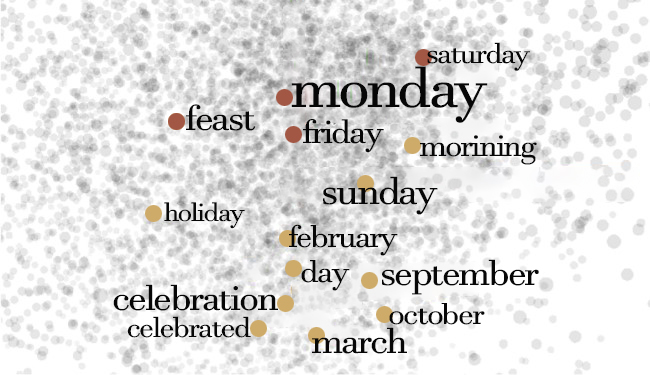
\includegraphics[width=6cm]{./Chapter5/Figures/word-graph.jpg}
\caption{分布式表示的可视化}
\label{fig:5-66}
\end{figure}
%-------------------------------------------

\parinterval  语言模型的词嵌入是通过词嵌入矩阵进行存储的,矩阵中的每一行对应了一个词的分布式表示结果。图\ref{fig:5-67}展示了一个词嵌入矩阵的实例。

%----------------------------------------------
\begin{figure}[htp]
\centering
%%%------------------------------------------------------------------------------------------------------------
\begin{tikzpicture}
\begin{scope}
\node [anchor=center,inner sep=2pt] (e) at (0,0) {\small{$e=w$}};
\node [anchor=west,inner sep=2pt] (c) at (e.east) {\small{$\textbf{C}$}};

\begin{pgfonlayer}{background}
\node [rectangle,inner sep=0.4em,draw,fill=blue!20!white] [fit = (e) (c)] (box) {};
\end{pgfonlayer}

\draw [->,thick] ([yshift=-1em]box.south)--([yshift=-0.1em]box.south) node [pos=0,below] (bottom1) {\small{单词$w$}};
\draw [->,thick] ([yshift=0.1em]box.north)--([yshift=1em]box.north) node [pos=1,above] (top1) {\scriptsize{$e$=(8,.2,-1,.9,...,1)}};
\node [anchor=north] (bottom2) at ([yshift=0.3em]bottom1.south) {\scriptsize{$w$=(0,0,1,0,...,0)}};
\node [anchor=south] (top2) at ([yshift=-0.3em]top1.north) {\small{$w$的分布式表示}};

{
\node [anchor=north west,fill=red!20!white] (cmatrix) at ([xshift=3em,yshift=1.0em]c.north east) {\scriptsize{$\begin{pmatrix} 1 & .2 & -.2 & 8 & ... & 0 \\ .6 & .8 & -2 & 1 & ... & -.2 \\ 8 & .2 & -1 & .9 & ... & 2.3 \\ 1 & 1.2 & -.9 & 3 & ... & .2 \\ ... & ... & ... & ... & ... & ... \\ 1 & .3 & 3 & .9 & ... & 5.1 \end{pmatrix}$}};
\node [anchor=west,inner sep=2pt,fill=red!30!white] (c) at (e.east) {\small{$\textbf{C}$}};
\draw [<-,thick] (c.east) -- ([xshift=3em]c.east);
}

{
\node [anchor=south,draw,fill=green!20!white] (e2) at ([yshift=1.5em]cmatrix.north) {\scriptsize{外部词嵌入系统得到的$\textbf{C}$}};
\draw [->,very thick,dashed] (e2.south) -- (cmatrix.north);
}

\end{scope}
\end{tikzpicture}
%%%------------------------------------------------------------------------------------------------------------


\caption{词嵌入矩阵$mathbf C$}
\label{fig:5-67}
\end{figure}
%-------------------------------------------

\parinterval  通常,有两种方法得到词嵌入矩阵。一种方法是把词嵌入作为语言模型的一部分进行训练,不过由于语言模型往往较复杂,这种方法非常耗时;另一种方法使用更加轻便的外部训练方法,如word2vec\cite{mikolov2013distributed}、Glove\cite{pennington2014glove}等。由于这些方法的效率较高,因此可以使用更大规模的数据得到更好的词嵌入结果。

%----------------------------------------------------------------------------------------
%    NEW SUB-SECTION
%----------------------------------------------------------------------------------------

\subsection{句子表示模型及预训练}

\parinterval  目前,词嵌入已经成为诸多自然语言处理系统的标配,也衍生出很多有趣的研究法方向,甚至有人开玩笑的喊出``embed everything''的口号。但是,冷静地看,词嵌入依旧存在一些问题:每个词都对应唯一的向量表示,那么对于一词多义现象,词义需要通过上下文进行区分,这时使用简单的词嵌入式是无法处理的。有一个著名的例子:

\begin{example}
Jobs was the CEO of {\red{\underline{apple}}}.

\qquad \qquad \; He finally ate the {\red{\underline{apple}}}.
\end{example}

\parinterval  这两句中``apple''的语义显然是不同的,第一句中的上下文``Jobs''和``CEO''可以帮助我们判断``apple''是一个公司名字,而不是水果。但是词嵌入只有一个结果,因此无法区分这两种情况。这个例子给我们一个启发:在一个句子中,不能孤立的看待单词,应同时考虑其上下文的信息。也就是需要一个能包含句子中上下文信息的表示模型。

%----------------------------------------------------------------------------------------
%    NEW SUBSUB-SECTION
%----------------------------------------------------------------------------------------

\subsubsection{简单的上下文表示模型}

\parinterval  回忆一下神经语言模型的结构,它需要在每个位置预测单词生成的概率。这个概率是由若干层神经网络进行计算后,通过输出层得到的。实际上,在送入输出层之前,系统已经得到了这个位置的一个向量(隐藏层的输出),因此可以把它看作是含有一部分上下文信息的表示结果。以RNN为例,图\ref{fig:5-68}展示了一个由四个词组成的句子,这里使用了一个两层循环神经网络对其进行建模。可以看到,对于第三个位置,RNN已经积累了从第1个单词到第3个单词的信息,因此可以看作是单词1-3(``乔布斯\ 就职\ 于'')的一种表示;另一方面,第4个单词的词嵌入可以看作是``苹果''自身的表示。这样,可以把第3 个位置RNN的输出和第4个位置的词嵌入进行合并,就得到了第4个位置上含有上下文信息的表示结果。从另一个角度说,这里得到了``苹果''的一种新的表示,它不仅包含苹果这个词自身的信息,也包含它前文的信息。

%----------------------------------------------
\begin{figure}[htp]
\centering
\begin{tikzpicture}
\begin{scope}
\tikzstyle{rnnnode} = [draw,inner sep=5pt,minimum width=4em,minimum height=1.5em,fill=green!30!white,blur shadow={shadow xshift=1pt,shadow yshift=-1pt}]
\node [anchor=west,rnnnode] (node11) at (0,0) {\scriptsize{RNN Cell}};
\node [anchor=west,rnnnode] (node12) at ([xshift=2em]node11.east) {\scriptsize{RNN Cell}};
\node [anchor=west,rnnnode] (node13) at ([xshift=2em]node12.east) {\scriptsize{RNN Cell}};
\node [anchor=west,rnnnode] (node14) at ([xshift=2em]node13.east) {\scriptsize{RNN Cell}};

\node [anchor=north,rnnnode,fill=red!30!white] (e1) at ([yshift=-1.2em]node11.south) {\scriptsize{embedding}};
\node [anchor=north,rnnnode,fill=red!30!white] (e2) at ([yshift=-1.2em]node12.south) {\scriptsize{embedding}};
\node [anchor=north,rnnnode,fill=red!30!white] (e3) at ([yshift=-1.2em]node13.south) {\scriptsize{embedding}};
\node [anchor=north,rnnnode,fill=red!30!white] (e4) at ([yshift=-1.2em]node14.south) {\scriptsize{embedding}};
\node [anchor=north] (w1) at ([yshift=-1em]e1.south) {\footnotesize{乔布斯}};
\node [anchor=north] (w2) at ([yshift=-1em]e2.south) {\footnotesize{任职}};
\node [anchor=north] (w3) at ([yshift=-1em]e3.south) {\footnotesize{于}};
\node [anchor=north] (w4) at ([yshift=-1em]e4.south) {\footnotesize{苹果}};

\draw [->,thick] ([yshift=0.1em]w1.north)--([yshift=-0.1em]e1.south);
\draw [->,thick] ([yshift=0.1em]w2.north)--([yshift=-0.1em]e2.south);
\draw [->,thick] ([yshift=0.1em]w3.north)--([yshift=-0.1em]e3.south);
\draw [->,thick] ([yshift=0.1em]w4.north)--([yshift=-0.1em]e4.south);

\draw [->,thick] ([yshift=0.1em]e1.north)--([yshift=-0.1em]node11.south);
\draw [->,thick] ([yshift=0.1em]e2.north)--([yshift=-0.1em]node12.south);
\draw [->,thick] ([yshift=0.1em]e3.north)--([yshift=-0.1em]node13.south);
\draw [->,thick] ([yshift=0.1em]e4.north)--([yshift=-0.1em]node14.south);

\node [anchor=south,rnnnode] (node21) at ([yshift=1.5em]node11.north) {\scriptsize{RNN Cell}};
\node [anchor=south,rnnnode] (node22) at ([yshift=1.5em]node12.north) {\scriptsize{RNN Cell}};
\node [anchor=south,rnnnode] (node23) at ([yshift=1.5em]node13.north) {\scriptsize{RNN Cell}};
\node [anchor=south,rnnnode] (node24) at ([yshift=1.5em]node14.north) {\scriptsize{RNN Cell}};

\node [anchor=south] (node31) at ([yshift=1.0em]node21.north) {\scriptsize{的表示}};
\node [anchor=south west] (node31new) at ([yshift=-0.3em]node31.north west) {\scriptsize{``乔布斯''}};
\node [anchor=south] (node32) at ([yshift=1.0em]node22.north) {\scriptsize{的表示\ \ \ }};
\node [anchor=south west] (node32new) at ([yshift=-0.3em]node32.north west) {\scriptsize{``乔布斯 任职''}};
\node [anchor=south] (node33) at ([yshift=1.0em]node23.north) {\scriptsize{的表示\ \ \ \ \ \ \ \ }};
\node [anchor=south west] (node33new) at ([yshift=-0.3em]node33.north west) {\scriptsize{``乔布斯 任职 于''}};
\node [anchor=south] (node34) at ([yshift=1.0em]node24.north) {\scriptsize{的表示\ \ \ \ \ \ \ \ }};
\node [anchor=south west] (node34new) at ([yshift=-0.3em]node34.north west) {\scriptsize{``乔布斯 任职 于 苹果''}};

\draw [->,thick] ([yshift=0.1em]node21.north)--([yshift=-0.1em]node31.south);
\draw [->,thick] ([yshift=0.1em]node22.north)--([yshift=-0.1em]node32.south);
\draw [->,thick] ([yshift=0.1em]node23.north)--([yshift=-0.1em]node33.south);
\draw [->,thick] ([yshift=0.1em]node24.north)--([yshift=-0.1em]node34.south);

\draw [->,thick] ([xshift=-1em]node21.west)--([xshift=-0.1em]node21.west);
\draw [->,thick] ([xshift=0.1em]node21.east)--([xshift=-0.1em]node22.west);
\draw [->,thick] ([xshift=0.1em]node22.east)--([xshift=-0.1em]node23.west);
\draw [->,thick] ([xshift=0.1em]node23.east)--([xshift=-0.1em]node24.west);
\draw [->,thick] ([xshift=0.1em]node24.east)--([xshift=1em]node24.east);

\draw [->,thick] ([yshift=0.1em]node11.north)--([yshift=-0.1em]node21.south);
\draw [->,thick] ([yshift=0.1em]node12.north)--([yshift=-0.1em]node22.south);
\draw [->,thick] ([yshift=0.1em]node13.north)--([yshift=-0.1em]node23.south);
\draw [->,thick] ([yshift=0.1em]node14.north)--([yshift=-0.1em]node24.south);

\draw [->,thick] ([xshift=-1em]node11.west)--([xshift=-0.1em]node11.west);
\draw [->,thick] ([xshift=0.1em]node11.east)--([xshift=-0.1em]node12.west);
\draw [->,thick] ([xshift=0.1em]node12.east)--([xshift=-0.1em]node13.west);
\draw [->,thick] ([xshift=0.1em]node13.east)--([xshift=-0.1em]node14.west);
\draw [->,thick] ([xshift=0.1em]node14.east)--([xshift=1em]node14.east);

{
\node [anchor=south] (toplabel1) at ([yshift=2em,xshift=-1.3em]node32new.north) {\footnotesize{``苹果''的表示:}};
\node [anchor=west,fill=blue!20!white,minimum width=3em] (toplabel2) at (toplabel1.east) {\footnotesize{上下文}};
}
{
\node [anchor=west,fill=red!20!white,minimum width=3em] (toplabel3) at (toplabel2.east) {\footnotesize{词}};
}

\begin{pgfonlayer}{background}
{
\node [rectangle,inner sep=2pt,draw,thick,dashed,red] [fit = (e4)] (r2) {};
\draw [->,thick,red] (r2.west) .. controls +(west:0.8) and +(south:2) .. ([xshift=1.3em]toplabel3.south);
}
{
\node [rectangle,inner sep=2pt,draw,thick,dashed,ublue,fill=white] [fit = (node33) (node33new)] (r1) {};
\draw [->,thick,ublue] ([xshift=-2em]r1.north) .. controls +(north:0.7) and +(south:0.7) .. ([xshift=-0.5em]toplabel2.south);
}
\end{pgfonlayer}

\end{scope}
\end{tikzpicture}
\caption{基于RNN的表示模型(词+上下文)}
\label{fig:5-68}
\end{figure}
%-------------------------------------------

\parinterval  在自然语言处理中,{\small\sffamily\bfseries{句子表示模型}}\index{句子表示模型}是指把输入的句子进行分布式表示。不过表示的形式不一定是一个单独的向量。现在广泛使用的句子表示模型可以被描述为:给定一个输入的句子$ \{ w_1,\dots ,w_m\} $,得到一个表示序列$ \{ \mathbf h_1,\dots ,\mathbf h_m\} $,其中$ h_i $是句子在第$ i $个位置的表示结果。$ \{ \mathbf h_1,\dots ,\mathbf h_m\} $就被看作是{\small\sffamily\bfseries{句子的表示}}\index{句子的表示},它可以被送入下游模块。比如,在机器翻译任务中,可以用这种模型表示源语言句子,然后通过这种表示结果进行目标语译文的生成;在序列标注(如词性标注)任务中,可以对输入的句子进行表示,然后在这个表示之上构建标签预测模块。很多自然语言处理任务都可以用句子表示模型进行建模,因此句子的表示模型也是应用最广泛的深度学习模型之一。而学习这种表示的过程也被称作{\small\sffamily\bfseries{表示学习}}\index{表示学习}(Representation Learning)\index{Representation Learning}。

\parinterval  句子表示模型有两种训练方法。最简单的方法是把它作为目标系统中的一个模块进行训练,比如把句子表示模型作为机器翻译系统的一部分。也就是,并不单独训练句子表示模型,而是把它作为一个内部模块放到其他系统中。另一种方法是把句子表示作为独立的模块,用外部系统进行训练,之后把训练好的表示模型放入目标系统中,再进行微调。这种方法构成了一种新的范式:预训练+微调(pre-training + fine-tuning)。图\ref{fig:5-69}对比了这两种不同的方法。

%----------------------------------------------
\begin{figure}[htp]
\centering
%%%------------------------------------------------------------------------------------------------------------
\begin{tikzpicture}

\begin{scope}

\node [anchor=west,draw,thick,minimum width=4em,minimum height=1.7em,fill=blue!20] (encoder) at (0,0) {模块};
\node [anchor=south,minimum width=4em,minimum height=1.7em] (space) at ([yshift=0.3em]encoder.north) {\footnotesize{目标系统}};

\begin{pgfonlayer}{background}
\node [rectangle,draw,thick,fill=red!20] [fit = (encoder) (space)] (system) {};
\end{pgfonlayer}

\node [anchor=north] (data) at ([yshift=-1em]system.south) {\scriptsize{\textbf{目标任务有标注数据}}};
\draw [->,thick] (data.north) -- ([yshift=-0.1em]system.south);
\node [anchor=north] (label) at ([yshift=-0em]data.south) {\scriptsize{(a) standard method}};

\end{scope}

\begin{scope}[xshift=2.8in]

\node [anchor=west,draw,dashed,thick,minimum width=4em,minimum height=1.7em,fill=blue!20] (encoder) at (0,0) {模块};
\node [anchor=south,minimum width=4em,minimum height=1.7em] (space) at ([yshift=0.3em]encoder.north) {\footnotesize{目标系统}};
\node [anchor=center,draw,thick,minimum width=4em,minimum height=1.7em,fill=green!20] (encoderpre) at ([xshift=-7em]encoder.center) {\footnotesize{语言模型}};
\draw [->,thick] (encoderpre.east) -- (encoder.west);

\begin{pgfonlayer}{background}
\node [rectangle,draw,thick,fill=red!20] [fit = (encoder) (space)] (system) {};
\end{pgfonlayer}

\node [anchor=north] (data) at ([yshift=-1em]system.south) {\scriptsize{\textbf{目标任务有标注数据}}};
\draw [->,thick] (data.north) -- ([yshift=-0.1em]system.south);
\node [anchor=north] (data2) at ([yshift=-1em,xshift=-7em]system.south) {\scriptsize{\textbf{大规模无标注数据}}};
\draw [->,thick] (data2.north) -- ([yshift=-0.1em]encoderpre.south);
\node [anchor=north] (label) at ([yshift=-0em,xshift=-4em]data.south) {\scriptsize{(b) pre-training + fine-tuning}};

\end{scope}

\end{tikzpicture}
%%%------------------------------------------------------------------------------------------------------------


\caption{表示模型的训练方法(与目标任务联合训练 vs 用外部任务预训练)}
\label{fig:5-69}
\end{figure}
%-------------------------------------------

\parinterval  目前,句子表示模型的预训练方法在多项自然语言处理任务上取得了很好的效果。预训练模型也成为了当今自然语言处理中的热点方向,相关系统也在很多评测任务上刷榜。除了上面提到的简单的神经语言模型的方法,还有各式各样基于预训练的表示模型被提出。接下来,会简单介绍其中比较有代表性的三种模型$\ \dash\ $ELMO、 GPT 和BERT。

%----------------------------------------------------------------------------------------
%    NEW SUBSUB-SECTION
%----------------------------------------------------------------------------------------

\subsubsection{ELMO模型}

\parinterval  ELMO(Embedding from Language Models)掀起了基于语言模型的预训练的热潮\cite{peters2018deep}。ELMO的论文也获得了自然语言处理领域顶级会议NAACL2018的最佳论文。

\parinterval  在ELMO中,作者认为词的表示应该能够包含丰富的句子结构信息,并且能够对多义词进行建模。而传统的词嵌入(例如word2vec)是上下文无关的,所以他们利用语言模型来获得一个上下文相关的预训练表示。EMLO基于双向LSTM语言模型\footnote{ LSTM(Long Short-Term Memory),即长短时记忆模型,是一种循环神经网络结构。},由一个正向语言模型和一个反向语言模型构成,目标函数是最大化这两个方向语言模型的似然(图\ref{fig:5-70})。简单来说,ELMO就是一个预训练好的双向语言模型,对于每个句子都可以生成相应的句子表示结果,这个结果会作为输入的特征被送入下游任务中。比如,ELMO在问答、文本蕴含、情感分析等多个任务中都表现出非常好的效果。

%----------------------------------------------
\begin{figure}[htp]
\centering
%%%------------------------------------------------------------------------------------------------------------
\begin{tikzpicture}
\begin{scope}[scale=1.2]

\node [anchor=west,draw,inner sep=4pt,fill=blue!20!white] (Lstm0) at (0,0) {\scriptsize{LSTM}};
\node [anchor=west,draw,inner sep=4pt,fill=blue!20!white] (Lstm1) at ([xshift=1em]Lstm0.east) {\scriptsize{LSTM}};
\node [anchor=west,inner sep=4pt] (sep) at ([xshift=0.5em]Lstm1.east) {\scriptsize{...}};
\node [anchor=west,draw,inner sep=4pt,fill=blue!20!white] (Lstm2) at ([xshift=0.5em]sep.east) {\scriptsize{LSTM}};

\node [anchor=south,draw,inner sep=4pt,fill=blue!20!white] (Lstm3) at ([yshift=1em]Lstm0.north) {\scriptsize{LSTM}};
\node [anchor=west,draw,inner sep=4pt,fill=blue!20!white] (Lstm4) at ([xshift=1em]Lstm3.east) {\scriptsize{LSTM}};
\node [anchor=west,inner sep=4pt] (sep1) at ([xshift=0.5em]Lstm4.east) {\scriptsize{...}};
\node [anchor=west,draw,inner sep=4pt,fill=blue!20!white] (Lstm5) at ([xshift=0.5em]sep1.east) {\scriptsize{LSTM}};

\node [rectangle,rounded corners,draw=black!50,densely dashed,inner sep=0.4em] [fit = (Lstm0) (Lstm2) (Lstm3) (Lstm5)] (inputshadow) {};

\node [anchor=north,draw,inner sep=4pt,fill=ugreen!20!white,minimum width=2em] (e1) at ([xshift=-2em,yshift=-1em]Lstm2.south) {\scriptsize{$\textbf{e}_1$}};
\node [anchor=west,draw,inner sep=4pt,fill=ugreen!20!white,minimum width=2em] (e2) at ([xshift=1em]e1.east) {\scriptsize{$\textbf{e}_2$}};
\node [anchor=west,inner sep=4pt] (sep5) at ([xshift=1em]e2.east) {\scriptsize{...}};
\node [anchor=west,draw,inner sep=4pt,fill=ugreen!20!white,minimum width=2em] (e3) at ([xshift=1em]sep5.east) {\scriptsize{$\textbf{e}_m$}};
\node [anchor=south] (word1) at ([yshift=-1.5em]e1.south) {\footnotesize {Once}};
\node [anchor=south] (word2) at ([yshift=-1.6em]e2.south) {\footnotesize {upon}};
\node [anchor=south] (wordseq) at ([yshift=-1.5em]sep5.south) {\footnotesize{...}};
\node [anchor=south] (word3) at ([yshift=-1.5em]e3.south) {\footnotesize {island}};

\node [anchor=south,draw,inner sep=4pt,fill=yellow!30,minimum width=2em] (t1) at ([xshift=-2em,yshift=1em]Lstm5.north) {\scriptsize{$\textbf{h}_1$}};
\node [anchor=west,draw,inner sep=4pt,fill=yellow!30,minimum width=2em] (t2) at ([xshift=1em]t1.east) {\scriptsize{$\textbf{h}_2$}};
\node [anchor=west,inner sep=4pt] (sep6) at ([xshift=1em]t2.east) {\scriptsize{...}};
\node [anchor=west,draw,inner sep=4pt,fill=yellow!30,minimum width=2em] (t3) at ([xshift=1em]sep6.east) {\scriptsize{$\textbf{h}_m$}};

\node [anchor=west,draw,inner sep=4pt,fill=blue!20!white] (Lstm6) at ([xshift=1.5em]Lstm2.east) {\scriptsize{LSTM}};
\node [anchor=west,draw,inner sep=4pt,fill=blue!20!white] (Lstm7) at ([xshift=1em]Lstm6.east) {\scriptsize{LSTM}};
\node [anchor=west,inner sep=4pt] (sep3) at ([xshift=0.5em]Lstm7.east) {\scriptsize{...}};
\node [anchor=west,draw,inner sep=4pt,fill=blue!20!white] (Lstm8) at ([xshift=0.5em]sep3.east) {\scriptsize{LSTM}};

\node [anchor=south,draw,inner sep=4pt,fill=blue!20!white] (Lstm9) at ([yshift=1em]Lstm6.north) {\scriptsize{LSTM}};
\node [anchor=west,draw,inner sep=4pt,fill=blue!20!white] (Lstm10) at ([xshift=1em]Lstm9.east) {\scriptsize{LSTM}};
\node [anchor=west,inner sep=4pt] (sep4) at ([xshift=0.5em]Lstm10.east) {\scriptsize{...}};
\node [anchor=west,draw,inner sep=4pt,fill=blue!20!white] (Lstm11) at ([xshift=0.5em]sep4.east) {\scriptsize{LSTM}};

\node [rectangle,rounded corners,draw=black!50,densely dashed,inner sep=0.4em] [fit = (Lstm6) (Lstm8) (Lstm9) (Lstm11)] (inputshadow) {};

\draw [->] ([xshift=0.1em]Lstm0.east) -- ([xshift=-0.1em]Lstm1.west);
\draw [->] ([xshift=0.1em]Lstm1.east) -- ([xshift=0.1em]sep.west);
\draw [->] ([xshift=-0.1em]sep.east) -- ([xshift=-0.1em]Lstm2.west);

\draw [->] ([xshift=0.1em]Lstm3.east) -- ([xshift=-0.1em]Lstm4.west);
\draw [->] ([xshift=0.1em]Lstm4.east) -- ([xshift=0.1em]sep1.west);
\draw [->] ([xshift=-0.1em]sep1.east) -- ([xshift=-0.1em]Lstm5.west);

\draw [->] ([yshift=0.1em]Lstm0.north) -- ([yshift=-0.1em]Lstm3.south);
\draw [->] ([yshift=0.1em]Lstm1.north) -- ([yshift=-0.1em]Lstm4.south);
\draw [->] ([yshift=0.1em]Lstm2.north) -- ([yshift=-0.1em]Lstm5.south);

\draw [->] ([xshift=-0.1em]Lstm7.west) -- ([xshift=0.1em]Lstm6.east);
\draw [->] ([xshift=0.1em]sep3.west) -- ([xshift=0.1em]Lstm7.east);
\draw [->] ([xshift=-0.1em]Lstm8.west) -- ([xshift=-0.1em]sep3.east);

\draw [->] ([xshift=-0.1em]Lstm10.west) -- ([xshift=0.1em]Lstm9.east);
\draw [->] ([xshift=0.1em]sep4.west) -- ([xshift=0.1em]Lstm10.east);
\draw [->] ([xshift=-0.1em]Lstm11.west) -- ([xshift=-0.1em]sep4.east);

\draw [->] ([yshift=0.1em]Lstm6.north) -- ([yshift=-0.1em]Lstm9.south);
\draw [->] ([yshift=0.1em]Lstm7.north) -- ([yshift=-0.1em]Lstm10.south);
\draw [->] ([yshift=0.1em]Lstm8.north) -- ([yshift=-0.1em]Lstm11.south);

\draw [->] ([yshift=0.1em]e1.north) -- ([yshift=-0.12em]Lstm0.south);
\draw [->] ([yshift=0.1em]e1.north) -- ([yshift=-0.12em]Lstm6.south);
\draw [->] ([yshift=0.1em]e2.north) -- ([yshift=-0.12em]Lstm1.south);
\draw [->] ([yshift=0.1em]e2.north) -- ([yshift=-0.12em]Lstm7.south);
\draw [->] ([yshift=0.1em]e3.north) -- ([yshift=-0.12em]Lstm2.south);
\draw [->] ([yshift=0.1em]e3.north) -- ([yshift=-0.12em]Lstm8.south);

\draw [->] ([yshift=0.1em]Lstm3.north) -- ([xshift=-0.05em,yshift=-0.12em]t1.south);
\draw [->] ([yshift=0.1em]Lstm9.north) -- ([yshift=-0.12em]t1.south);
\draw [->] ([yshift=0.1em]Lstm4.north) -- ([xshift=-0.05em,yshift=-0.12em]t2.south);
\draw [->] ([yshift=0.1em]Lstm10.north) -- ([yshift=-0.12em]t2.south);
\draw [->] ([yshift=0.1em]Lstm5.north) -- ([xshift=-0.05em,yshift=-0.12em]t3.south);
\draw [->] ([yshift=0.1em]Lstm11.north) -- ([yshift=-0.12em]t3.south);

\end{scope}
\end{tikzpicture}
%%%------------------------------------------------------------------------------------------------------------


\caption{ELMO模型结构}
\label{fig:5-70}
\end{figure}
%-------------------------------------------

%----------------------------------------------------------------------------------------
%    NEW SUBSUB-SECTION
%----------------------------------------------------------------------------------------

\subsubsection{GPT模型}

\parinterval  GPT(Generative Pre-Training)也是一种基于语言建模的句子表示模型\cite{radford2018improving}。该工作的贡献在于利用Transformer结构代替了LSTM。而且该模型基于Pre-training + Fine-tuning的框架,预训练的结果将作为下游系统的句子表示模块的参数初始值,因此可以更好的适应目标任务。

\parinterval  GPT模型仍然使用标准的语言建模的思路,即通过前$ n-1 $个词预测第$ n $个词。但是在网络结构上,GPT模型使用了Transformer(图\ref{fig:5-71}),而且模型参数会在目标任务上进行有监督的微调。与ELMO模型的做法不同,GPT不需要对目标任务构建新的模型结构,而是直接在Transformer语言表示模型的最后一层加上Softmax层作为任务的输出层。实验结果证明,GPT模型的性能较ELMO模型更为优越,在12个NLP任务中取得了9个任务当时最好的结果。

%----------------------------------------------
\begin{figure}[htp]
\centering
%%%------------------------------------------------------------------------------------------------------------
\begin{tikzpicture}
\begin{scope}[scale=1.2]

\node [anchor=west,draw,inner sep=4pt,fill=blue!20!white,minimum width=3em] (Trm0) at (0,0) {\scriptsize{TRM}};
\node [anchor=west,draw,inner sep=4pt,fill=blue!20!white,minimum width=3em] (Trm1) at ([xshift=1em]Trm0.east) {\scriptsize{TRM}};
\node [anchor=west,draw,inner sep=4pt,fill=blue!20!white,minimum width=3em] (Trm2) at ([xshift=1em]Trm1.east) {\scriptsize{TRM}};
\node [anchor=west,draw,inner sep=4pt,fill=blue!20!white,minimum width=3em] (Trm3) at ([xshift=1em]Trm2.east) {\scriptsize{TRM}};
\node [anchor=west,inner sep=4pt] (sep) at ([xshift=1em]Trm3.east) {\scriptsize{...}};
\node [anchor=west,draw,inner sep=4pt,fill=blue!20!white,minimum width=3em] (Trm4) at ([xshift=1em]sep.east) {\scriptsize{TRM}};

\node [anchor=south,draw,inner sep=4pt,fill=blue!20!white,minimum width=3em] (Trm5) at ([yshift=1.2em]Trm0.north) {\scriptsize{TRM}};
\node [anchor=west,draw,inner sep=4pt,fill=blue!20!white,minimum width=3em] (Trm6) at ([xshift=1em]Trm5.east) {\scriptsize{TRM}};
\node [anchor=west,draw,inner sep=4pt,fill=blue!20!white,minimum width=3em] (Trm7) at ([xshift=1em]Trm6.east) {\scriptsize{TRM}};
\node [anchor=west,draw,inner sep=4pt,fill=blue!20!white,minimum width=3em] (Trm8) at ([xshift=1em]Trm7.east) {\scriptsize{TRM}};
\node [anchor=west,inner sep=4pt] (sep1) at ([xshift=1em]Trm8.east) {\scriptsize{...}};
\node [anchor=west,draw,inner sep=4pt,fill=blue!20!white,minimum width=3em] (Trm9) at ([xshift=1em]sep1.east) {\scriptsize{TRM}};

\node [rectangle,rounded corners,draw=black!50,densely dashed,inner sep=0.4em] [fit = (Trm0) (Trm4) (Trm5) (Trm9)] (inputshadow) {};

\node [anchor=north,draw,inner sep=4pt,fill=ugreen!20!white,minimum width=2em] (e1) at ([yshift=-1.2em]Trm0.south) {\scriptsize{$\textbf{e}_1$}};
\node [anchor=north,draw,inner sep=4pt,fill=ugreen!20!white,minimum width=2em] (e2) at ([yshift=-1.2em]Trm1.south) {\scriptsize{$\textbf{e}_2$}};
\node [anchor=north,draw,inner sep=4pt,fill=ugreen!20!white,minimum width=2em] (e3) at ([yshift=-1.2em]Trm2.south) {\scriptsize{$\textbf{e}_3$}};
\node [anchor=north,draw,inner sep=4pt,fill=ugreen!20!white,minimum width=2em] (e4) at ([yshift=-1.2em]Trm3.south) {\scriptsize{$\textbf{e}_4$}};
\node [anchor=north,inner sep=4pt] (sep5) at ([yshift=-1em]sep.south) {\scriptsize{...}};
\node [anchor=north,draw,inner sep=4pt,fill=ugreen!20!white,minimum width=2em] (e5) at ([yshift=-1.2em]Trm4.south) {\scriptsize{$\textbf{e}_m$}};
\node [anchor=south] (word1) at ([yshift=-1.5em]e1.south) {\footnotesize {Once}};
\node [anchor=south] (word2) at ([yshift=-1.6em]e2.south) {\footnotesize {upon}};
\node [anchor=south] (word3) at ([yshift=-1.5em]e3.south) {\footnotesize {a}};
\node [anchor=south] (word4) at ([yshift=-1.5em]e4.south) {\footnotesize {time}};
\node [anchor=south] (wordseq) at ([yshift=-2.0em]sep5.south) {\footnotesize{...}};
\node [anchor=south] (word4) at ([yshift=-1.5em]e5.south) {\footnotesize {island}};

\node [anchor=south,draw,inner sep=4pt,fill=yellow!30,minimum width=2em] (t1) at ([yshift=1.2em]Trm5.north) {\scriptsize{$\textbf{h}_1$}};
\node [anchor=south,draw,inner sep=4pt,fill=yellow!30,minimum width=2em] (t2) at ([yshift=1.2em]Trm6.north) {\scriptsize{$\textbf{h}_2$}};
\node [anchor=south,draw,inner sep=4pt,fill=yellow!30,minimum width=2em] (t3) at ([yshift=1.2em]Trm7.north) {\scriptsize{$\textbf{h}_3$}};
\node [anchor=south,draw,inner sep=4pt,fill=yellow!30,minimum width=2em] (t4) at ([yshift=1.2em]Trm8.north) {\scriptsize{$\textbf{h}_4$}};
\node [anchor=south,inner sep=4pt] (sep6) at ([yshift=1em]sep1.north) {\scriptsize{...}};
\node [anchor=south,draw,inner sep=4pt,fill=yellow!30,minimum width=2em] (t5) at ([yshift=1.2em]Trm9.north) {\scriptsize{$\textbf{h}_m$}};

\node [anchor=west,draw,inner sep=3pt,fill=blue!20!white,minimum width=1em] (Lt1) at ([yshift=1.2em]t1.west) {\tiny{TRM}};
\node [anchor=west] (Lt2) at ([xshift=-0.1em]Lt1.east) {\tiny{: Transformer}};

\draw [->] ([yshift=0.1em]e1.north) -- ([yshift=-0.1em]Trm0.south);
\draw [->] ([yshift=0.1em]e1.north) -- ([yshift=-0.1em]Trm1.260);
\draw [->] ([yshift=0.1em]e1.north) -- ([yshift=-0.1em]Trm2.260);
\draw [->] ([yshift=0.1em]e1.north) -- ([yshift=-0.1em]Trm3.260);
\draw [->] ([yshift=0.1em]e1.north) -- ([yshift=-0.1em]Trm4.260);
\draw [->] ([yshift=0.1em]e2.north) -- ([yshift=-0.1em]Trm1.south);

\draw [->] ([yshift=0.1em]e3.north) -- ([yshift=-0.1em]Trm2.south);
\draw [->] ([yshift=0.1em]e3.north) -- ([yshift=-0.1em]Trm3.260);
\draw [->] ([yshift=0.1em]e3.north) -- ([yshift=-0.1em]Trm4.260);
\draw [->] ([yshift=0.1em]e4.north) -- ([yshift=-0.1em]Trm3.south);
\draw [->] ([yshift=0.1em]e5.north) -- ([yshift=-0.1em]Trm4.south);

\draw [->] ([yshift=0.1em]Trm0.north) -- ([yshift=-0.1em]Trm5.south);
\draw [->] ([yshift=0.1em]Trm0.north) -- ([yshift=-0.1em]Trm6.260);
\draw [->] ([yshift=0.1em]Trm0.north) -- ([yshift=-0.1em]Trm7.260);
\draw [->] ([yshift=0.1em]Trm0.north) -- ([yshift=-0.1em]Trm8.260);
\draw [->] ([yshift=0.1em]Trm0.north) -- ([yshift=-0.1em]Trm9.260);
\draw [->] ([yshift=0.1em]Trm1.north) -- ([yshift=-0.1em]Trm6.south);
\draw [->] ([yshift=0.1em]Trm2.north) -- ([yshift=-0.1em]Trm7.south);
\draw [->] ([yshift=0.1em]Trm2.north) -- ([yshift=-0.1em]Trm8.260);
\draw [->] ([yshift=0.1em]Trm2.north) -- ([yshift=-0.1em]Trm9.260);
\draw [->] ([yshift=0.1em]Trm3.north) -- ([yshift=-0.1em]Trm8.south);
\draw [->] ([yshift=0.1em]Trm4.north) -- ([yshift=-0.1em]Trm9.south);

\draw [->] ([yshift=0.1em]Trm5.north) -- ([yshift=-0.1em]t1.south);
\draw [->] ([yshift=0.1em]Trm6.north) -- ([yshift=-0.1em]t2.south);
\draw [->] ([yshift=0.1em]Trm7.north) -- ([yshift=-0.1em]t3.south);
\draw [->] ([yshift=0.1em]Trm8.north) -- ([yshift=-0.1em]t4.south);
\draw [->] ([yshift=0.1em]Trm9.north) -- ([yshift=-0.1em]t5.south);

\end{scope}
\end{tikzpicture}
%%%------------------------------------------------------------------------------------------------------------


\caption{GPT模型结构}
\label{fig:5-71}
\end{figure}
%-------------------------------------------
\vspace{-0.5em}
%----------------------------------------------------------------------------------------
%    NEW SUBSUB-SECTION
%----------------------------------------------------------------------------------------

\subsubsection{BERT模型}

\parinterval  BERT(Bidirectional Encoder Representations from Transformers)是另一个非常有代表性的基于预训练的句子表示模型\cite{DBLP:conf/naacl/DevlinCLT19}。某种意义上,BERT把基于预训练的句子表示模型推向了新的高潮。BERT的论文也获得了NAACL2019最佳论文奖。

\parinterval  与传统语言模型的训练目标不同,BERT不使用预测下一个词作为训练目标,而是提出了两个新的任务。

\begin{itemize}
\vspace{0.5em}
\item 第一个任务被称为Masked LM。在输入的词序列中随机地挡住一定量的的词(比如15\%的单词被挡住),然后让模型去预测挡住的这些词。这个过程有些类似于英语考试中的完形填空。这么做的好处是,模型能够从多个方向去预测这些被遮罩住的词(图\ref{fig:5-72}),而不是像传统语言模型一样从单个方向预测(自左向右或者自右向左)。Masked LM的思想也影响了很多预训练模型的设计。
\vspace{0.5em}
\item 第二个任务是预测下一个句子。当选择句子a与b作为预训练样本时,b有一半几率可能是a的下一句,也有一半几率来自语料库的随机句子,从而可以更好地学习句子之间的相关性。
\vspace{0.5em}
\end{itemize}

\parinterval  BERT的训练目标就是最小化这两个任务上的损失函数。实验结果证明,BERT\\模型的性能十分强劲,在11个NLP任务上取得了当时最好的性能。

%----------------------------------------------
\begin{figure}[htp]
\centering
%%%------------------------------------------------------------------------------------------------------------
\begin{tikzpicture}
\begin{scope}[scale=1.2]

\node [anchor=west,draw,inner sep=4pt,fill=blue!20!white,minimum width=3em] (Trm0) at (0,0) {\scriptsize{TRM}};
\node [anchor=west,draw,inner sep=4pt,fill=blue!20!white,minimum width=3em] (Trm1) at ([xshift=1em]Trm0.east) {\scriptsize{TRM}};
\node [anchor=west,draw,inner sep=4pt,fill=blue!20!white,minimum width=3em] (Trm2) at ([xshift=1em]Trm1.east) {\scriptsize{TRM}};
\node [anchor=west,draw,inner sep=4pt,fill=blue!20!white,minimum width=3em] (Trm3) at ([xshift=1em]Trm2.east) {\scriptsize{TRM}};
\node [anchor=west,inner sep=4pt] (sep) at ([xshift=1em]Trm3.east) {\scriptsize{...}};
\node [anchor=west,draw,inner sep=4pt,fill=blue!20!white,minimum width=3em] (Trm4) at ([xshift=1em]sep.east) {\scriptsize{TRM}};

\node [anchor=south,draw,inner sep=4pt,fill=blue!20!white,minimum width=3em] (Trm5) at ([yshift=1.2em]Trm0.north) {\scriptsize{TRM}};
\node [anchor=west,draw,inner sep=4pt,fill=blue!20!white,minimum width=3em] (Trm6) at ([xshift=1em]Trm5.east) {\scriptsize{TRM}};
\node [anchor=west,draw,inner sep=4pt,fill=blue!20!white,minimum width=3em] (Trm7) at ([xshift=1em]Trm6.east) {\scriptsize{TRM}};
\node [anchor=west,draw,inner sep=4pt,fill=blue!20!white,minimum width=3em] (Trm8) at ([xshift=1em]Trm7.east) {\scriptsize{TRM}};
\node [anchor=west,inner sep=4pt] (sep1) at ([xshift=1em]Trm8.east) {\scriptsize{...}};
\node [anchor=west,draw,inner sep=4pt,fill=blue!20!white,minimum width=3em] (Trm9) at ([xshift=1em]sep1.east) {\scriptsize{TRM}};

\node [rectangle,rounded corners,draw=black!50,densely dashed,inner sep=0.4em] [fit = (Trm0) (Trm4) (Trm5) (Trm9)] (inputshadow) {};

\node [anchor=north,draw,inner sep=4pt,fill=ugreen!20!white,minimum width=2em] (e1) at ([yshift=-1.2em]Trm0.south) {\scriptsize{$\textbf{e}_1$}};
\node [anchor=north,draw,inner sep=4pt,fill=ugreen!20!white,minimum width=2em] (e2) at ([yshift=-1.2em]Trm1.south) {\scriptsize{$\textbf{e}_2$}};
\node [anchor=north,draw,inner sep=4pt,fill=ugreen!20!white,minimum width=2em] (e3) at ([yshift=-1.2em]Trm2.south) {\scriptsize{$\textbf{e}_3$}};
\node [anchor=north,draw,inner sep=4pt,fill=ugreen!20!white,minimum width=2em] (e4) at ([yshift=-1.2em]Trm3.south) {\scriptsize{$\textbf{e}_4$}};
\node [anchor=north,inner sep=4pt] (sep5) at ([yshift=-1em]sep.south) {\scriptsize{...}};
\node [anchor=north,draw,inner sep=4pt,fill=ugreen!20!white,minimum width=2em] (e5) at ([yshift=-1.2em]Trm4.south) {\scriptsize{$\textbf{e}_m$}};
\node [anchor=south] (word1) at ([yshift=-1.5em]e1.south) {\footnotesize {Once}};
\node [anchor=south] (word2) at ([yshift=-1.7em]e2.south) {\footnotesize {[MASK]}};
\node [anchor=south] (word3) at ([yshift=-1.5em]e3.south) {\footnotesize {a}};
\node [anchor=south] (word4) at ([yshift=-1.5em]e4.south) {\footnotesize {time}};
\node [anchor=south] (wordseq) at ([yshift=-2.0em]sep5.south) {\footnotesize{...}};
\node [anchor=south] (word4) at ([yshift=-1.5em]e5.south) {\footnotesize {island}};

\node [anchor=south,draw,inner sep=4pt,fill=yellow!30,minimum width=2em] (t1) at ([yshift=1.2em]Trm5.north) {\scriptsize{$\textbf{h}_1$}};
\node [anchor=south,draw,inner sep=4pt,fill=yellow!30,minimum width=2em] (t2) at ([yshift=1.2em]Trm6.north) {\scriptsize{$\textbf{h}_2$}};
\node [anchor=south,draw,inner sep=4pt,fill=yellow!30,minimum width=2em] (t3) at ([yshift=1.2em]Trm7.north) {\scriptsize{$\textbf{h}_3$}};
\node [anchor=south,draw,inner sep=4pt,fill=yellow!30,minimum width=2em] (t4) at ([yshift=1.2em]Trm8.north) {\scriptsize{$\textbf{h}_4$}};
\node [anchor=south,inner sep=4pt] (sep6) at ([yshift=1em]sep1.north) {\scriptsize{...}};
\node [anchor=south,draw,inner sep=4pt,fill=yellow!30,minimum width=2em] (t5) at ([yshift=1.2em]Trm9.north) {\scriptsize{$\textbf{h}_m$}};

\node [anchor=west,draw,inner sep=3pt,fill=blue!20!white,minimum width=1em] (Lt1) at ([yshift=1.2em]t1.west) {\tiny{TRM}};
\node [anchor=west] (Lt2) at ([xshift=-0.1em]Lt1.east) {\tiny{: Transformer}};

\draw [->] ([yshift=0.1em]e1.north) -- ([yshift=-0.1em]Trm0.south);
\draw [->] ([yshift=0.1em]e1.north) -- ([yshift=-0.1em]Trm1.south);
\draw [->] ([yshift=0.1em]e1.north) -- ([yshift=-0.1em]Trm2.south);
\draw [->] ([yshift=0.1em]e1.north) -- ([yshift=-0.1em]Trm3.south);
\draw [->] ([yshift=0.1em]e1.north) -- ([yshift=-0.1em]Trm4.south);
\draw [->] ([yshift=0.1em]e2.north) -- ([yshift=-0.1em]Trm1.south);
\draw [->] ([yshift=0.1em]e3.north) -- ([yshift=-0.1em]Trm0.south);
\draw [->] ([yshift=0.1em]e3.north) -- ([yshift=-0.1em]Trm1.south);
\draw [->] ([yshift=0.1em]e3.north) -- ([yshift=-0.1em]Trm2.south);
\draw [->] ([yshift=0.1em]e3.north) -- ([yshift=-0.1em]Trm3.south);
\draw [->] ([yshift=0.1em]e3.north) -- ([yshift=-0.1em]Trm4.south);
\draw [->] ([yshift=0.1em]e4.north) -- ([yshift=-0.1em]Trm3.south);
\draw [->] ([yshift=0.1em]e5.north) -- ([yshift=-0.1em]Trm4.south);

\draw [->] ([yshift=0.1em]Trm0.north) -- ([yshift=-0.1em]Trm5.south);
\draw [->] ([yshift=0.1em]Trm0.north) -- ([yshift=-0.1em]Trm6.south);
\draw [->] ([yshift=0.1em]Trm0.north) -- ([yshift=-0.1em]Trm8.south);
\draw [->] ([yshift=0.1em]Trm0.north) -- ([yshift=-0.1em]Trm9.south);
\draw [->] ([yshift=0.1em]Trm1.north) -- ([yshift=-0.1em]Trm6.south);
\draw [->] ([yshift=0.1em]Trm2.north) -- ([yshift=-0.1em]Trm5.south);
\draw [->] ([yshift=0.1em]Trm2.north) -- ([yshift=-0.1em]Trm6.south);
\draw [->] ([yshift=0.1em]Trm2.north) -- ([yshift=-0.1em]Trm7.south);
\draw [->] ([yshift=0.1em]Trm2.north) -- ([yshift=-0.1em]Trm8.south);
\draw [->] ([yshift=0.1em]Trm2.north) -- ([yshift=-0.1em]Trm9.south);
\draw [->] ([yshift=0.1em]Trm3.north) -- ([yshift=-0.1em]Trm8.south);
\draw [->] ([yshift=0.1em]Trm4.north) -- ([yshift=-0.1em]Trm9.south);

\draw [->] ([yshift=0.1em]Trm5.north) -- ([yshift=-0.1em]t1.south);
\draw [->] ([yshift=0.1em]Trm6.north) -- ([yshift=-0.1em]t2.south);
\draw [->] ([yshift=0.1em]Trm7.north) -- ([yshift=-0.1em]t3.south);
\draw [->] ([yshift=0.1em]Trm8.north) -- ([yshift=-0.1em]t4.south);
\draw [->] ([yshift=0.1em]Trm9.north) -- ([yshift=-0.1em]t5.south);

\end{scope}
\end{tikzpicture}
%%%------------------------------------------------------------------------------------------------------------


\caption{BERT模型结构}
\label{fig:5-72}
\end{figure}
%-------------------------------------------
\vspace{-0.5em}

%----------------------------------------------------------------------------------------
%    NEW SUUBSUB-SECTION
%----------------------------------------------------------------------------------------

\subsubsection{为什么要预训练?}

\parinterval  基于预训练的句子表示模型确实给自然语言处理带来了新的思路。相比传统的基于目标任务的建模和训练方法,预训练有如下优势:

\begin{itemize}
\vspace{0.5em}
\item 目标任务依赖有指导训练,但是带标注的数据往往十分有限。预训练模型并不依赖带标注数据,因此可以从更大规模的无标注数据(比如训练语言模型中使用的纯文本数据)学习知识,这使得预训练模型可以捕捉更加通用的语言规律,甚至有时候会具有一些``常识''\footnote{关于自然语言处理系统是否具有常识也存在不同的观点。从一些任务上的实验结果上看,很多模型确实能够进行一些常识性推理。但是,当问题的难度增加时,绝大多数模型还无法做到人类的水平。};
\vspace{0.5em}
\item 由于预训练并不依赖具体的目标任务,因此不会对目标任务产生过拟合,模型具有较好的泛化能力;
\vspace{0.5em}
\item 从优化的角度,预训练相当于将模型``初始化''到参数空间中优质解密度更高的区域(图\ref{fig:5-73}),下游任务更容易通过微调找到更好的参数(面向具体任务)。此外,也有实验表明预训练可以让模型参数落到损失函数曲面比较光滑的区域,这样能够避免下游任务在凸凹不平的损失函数曲面上陷入局部最优。
\vspace{0.5em}
\end{itemize}

%----------------------------------------------
\begin{figure}[htp]
\centering
%%%------------------------------------------------------------------------------------------------------------
\begin{tikzpicture}
\draw[name path=ellipse,thick] (0,0) circle[x radius = 2, y radius = 1];
\node[rectangle,minimum size=0.1em,inner sep=2pt,fill=red] (p1) at (0.2,0.5) {};
\node[rectangle,minimum size=0.1em,inner sep=2pt,fill=red] (p2) at (0.3,0.6) {};
\node[rectangle,minimum size=0.1em,inner sep=2pt,fill=red] (p3) at (0.1,-0.1) {};
\node[rectangle,minimum size=0.1em,inner sep=2pt,fill=red] (p4) at (0.4,0) {};
\node[rectangle,minimum size=0.1em,inner sep=2pt,fill=red] (p5) at (0.5,0.3) {};
\node[rectangle,minimum size=0.1em,inner sep=2pt,fill=red] (p6) at (0.6,0.1) {};
\node[rectangle,minimum size=0.1em,inner sep=2pt,fill=red] (p7) at (0.7,-0.1) {};
\node[rectangle,minimum size=0.1em,inner sep=2pt,fill=red] (p8) at (-1.2,0.4) {};
\node[rectangle,minimum size=0.1em,inner sep=2pt,fill=red] (p9) at (-1.0,-0.3) {};
\node[rectangle,minimum size=0.1em,inner sep=2pt,fill=red] (p10) at (-0.1,-0.8) {};

\begin{pgfonlayer}{background}
{
\node [rectangle,inner sep=0.4em,draw,blue] [fit = (p1) (p2) (p3) (p4) (p5) (p6)] (area) {};
}
\end{pgfonlayer}

\draw [->] (2.5,-0.7) -- (1.8,-0.5) node [pos=0,right] {\scriptsize{模型参数解空间}};

{
\draw [->] (2.0,0.7) -- (area.20) node [pos=0,right] {\scriptsize{优质解高密度区域(预训练)}};
}
{
\draw [->] (-2.0,0.7) -- (p8.west) node [pos=0,left] {\scriptsize{游离的解}};
}

\end{tikzpicture}
%%%------------------------------------------------------------------------------------------------------------


\caption{模型的参数空间}
\label{fig:5-73}
\end{figure}
%-------------------------------------------

%----------------------------------------------------------------------------------------
%    NEW SECTION
%----------------------------------------------------------------------------------------

\sectionnewpage
\section{小结及深入阅读}

\parinterval  神经网络为解决自然语言处理问题提供了全新的思路。而所谓深度学习也是建立在多层神经网络结构之上的一系列模型和方法。本章从神经网络的基本概念到其在语言建模中的应用进行了概述。由于篇幅所限,这里无法覆盖所有神经网络和深度学习的相关内容,感兴趣的读者可以进一步阅读《Neural Network Methods in Natural Language Processing》\cite{goldberg2017neural}和《Deep Learning》\cite{Goodfellow-et-al-2016}。此外,也有很多研究方向值得关注:

\begin{itemize}
\vspace{0.5em}
\item 端到端学习是神经网络方法的特点之一。这样,系统开发者不需要设计输入和输出的隐含结构,甚至连特征工程都不再需要。但是,另一方面,由于这种端到端学习完全由神经网络自行完成,整个学习过程没有人的先验知识做指导,导致学习的结构和参数很难进行解释。针对这个问题也有很多研究者进行{\small\sffamily\bfseries{可解释机器学习}}\index{可解释机器学习}(Explainable Machine Learning)\index{Explainable Machine Learning}的研究\cite{guidotti2018survey}\cite{koh2017understanding}。对于自然语言处理,方法的可解释性是十分必要的。从另一个角度说,如何使用先验知识改善端到端学习也是很多人关注的方向\cite{arthur2016incorporating}\cite{Zhang2017PriorKI},比如,如何使用句法知识改善自然语言处理模型\cite{zollmann2006syntax}\cite{charniak2003syntax}\cite{stahlberg2016syntactically}。
\vspace{0.5em}
\item 词嵌入是自然语言处理近些年的重要进展。所谓“嵌入”是一类方法,理论上,把一个事物进行分布式表示的过程都可以被看作是广义上的“嵌入”。基于这种思想的表示学习也成为了自然语言处理中的前沿方法。比如,如何对树结构,甚至图结构进行分布式表示\cite{plank2013embedding}\cite{perozzi2014deepwalk}成为了分析自然语言的重要方法。此外,除了语言建模,还有很多方式可以进行词嵌入的学习,比如,SENNA\cite{collobert2011natural}、word2vec\cite{mikolov2013efficient}\cite{mikolov2013distributed}、Glove\cite{pennington2014glove}、CoVe\cite{mccann2017learned}等。
\vspace{0.5em}
\item 预训练是表示学习的重要产物。预训练已经在图像处理等领域得到应用。在自然语言处理中,以BERT为代表的预训练模型席卷了很多自然语言处理任务,在阅读理解等比赛(如Stanford Question Answering)中已经成为了所有参赛系统的标配。除了ELMO、GPT、BERT,还有很多优秀的预训练模型,包括GPT-2\cite{radford2019language}、XLM\cite{lample2019cross}、MASS\cite{song2019mass}、XLNet\cite{yang2019xlnet},等等。但是,预训练往往依赖大规模的数据和并行运算设备,这使得很多普通研究者对训练这样的模型望而却步。不过,也有一些研究轻量的预训练方法,也受到了很多关注,例如ALBERT\cite{lan2019albert}。
\vspace{0.5em}
\end{itemize}

\include{Chapter6/chapter6}
\include{Chapter7/chapter7}
\include{ChapterAppend/chapterappend}


%----------------------------------------------------------------------------------------
%	BIBLIOGRAPHY
%----------------------------------------------------------------------------------------
\chapterimage{fig-NEU-10.jpg} % Image of the header
\cleardoublepage % Make sure the index starts on an odd (right side) page
\printbibliography


%----------------------------------------------------------------------------------------
%	INDEX
%----------------------------------------------------------------------------------------
\chapterimage{fig-NEU-10.jpg} % Image of the header
\cleardoublepage % Make sure the index starts on an odd (right side) page
%\phantomsection
%\setlength{\columnsep}{0.75cm} % Space between the 2 columns of the index
%\addcontentsline{toc}{chapter}{\textcolor{ocre}{Index}} % Add an Index heading to the table of contents
\printindex % Show index

%-------------------------

%\end{CJK}
\end{document}
